\documentclass[UTF8,10pt,twocolumn,openany]{ctexbook}

% ==============================================================================
% How to Design Programs (Second Edition) - 紧凑双栏中文排版宏包与样式配置
% ==============================================================================

% 字号配置：全局 9pt 紧凑版面
\usepackage[fontsize=9pt]{scrextend}

% 页面几何与边距（左右边距减半至 0.8cm，可用版心大幅扩展）
\usepackage[a4paper, top=1.8cm, bottom=1.8cm, left=0.8cm, right=0.8cm, headheight=13pt, footskip=18pt, columnsep=6.5mm]{geometry}
\setlength{\columnseprule}{0pt} % 去除双栏中线

% 数学与符号
\usepackage{amsmath, amssymb}
\usepackage{newunicodechar}
\newunicodechar{λ}{\ensuremath{\lambda}}
\newunicodechar{ε}{\ensuremath{\varepsilon}}
\newunicodechar{⊕}{\ensuremath{\oplus}}

% 颜色定义
\usepackage[x11names, svgnames, dvipsnames]{xcolor}
\definecolor{NavyTheme}{RGB}{24, 43, 73}        % 主题深蓝
\definecolor{AccentGreen}{RGB}{26, 127, 86}     % 配方绿
\definecolor{AccentPurple}{RGB}{103, 58, 183}   % 练习紫
\definecolor{AccentAmber}{RGB}{217, 119, 6}     % 注意橙
\definecolor{CodeBg}{RGB}{247, 248, 250}        % 代码背景浅灰
\definecolor{CodeFrame}{RGB}{220, 224, 230}     % 代码边框
\definecolor{ReplBg}{RGB}{243, 244, 246}        % REPL背景
\definecolor{TextDark}{RGB}{30, 41, 59}         % 正文字体深色
\definecolor{StepHl}{RGB}{216, 221, 230}        % 单步求值高亮底色
\definecolor{StepHlDeep}{RGB}{190, 197, 210}    % 嵌套作用域深高亮

% 图形与自适应双栏限宽
\usepackage{graphicx}
\usepackage[export]{adjustbox}
\graphicspath{{images/}}

% 拦截所有图片，保证在单栏内绝对不超出栏宽，保持纵横比
\let\oldincludegraphics\includegraphics
\RenewDocumentCommand{\includegraphics}{O{} m}{%
  \oldincludegraphics[#1, max width=\linewidth, keepaspectratio]{#2}%
}

\usepackage{caption}
\captionsetup{font=footnotesize, labelfont={bf, color=NavyTheme}, labelsep=quad, skip=3pt}

% 段落与列表紧凑化
\linespread{1.12}
\setlength{\parskip}{1.5pt plus 1pt minus 0.5pt}
\setlength{\parindent}{2\ccwd}
\usepackage{enumitem}
\setlist{itemsep=1.5pt, parsep=0.5pt, topsep=2.5pt, partopsep=0pt, leftmargin=1.5em}

% 页眉页脚
\usepackage{fancyhdr}
\pagestyle{fancy}
\fancyhf{}
\fancyhead[LE]{\small\color{gray}\nouppercase{\leftmark}}
\fancyhead[RO]{\small\color{gray}\nouppercase{\rightmark}}
\fancyfoot[C]{\small\thepage}
\renewcommand{\headrulewidth}{0.3pt}
\renewcommand{\footrulewidth}{0pt}

\fancypagestyle{plain}{
  \fancyhf{}
  \fancyfoot[C]{\small\thepage}
  \renewcommand{\headrulewidth}{0pt}
}

% 紧凑标题定制
\usepackage{titlesec}
\titleformat{\chapter}[block]
  {\normalfont\LARGE\bfseries\color{NavyTheme}}
  {\color{NavyTheme!70}\thechapter\quad}
  {0pt}
  {\LARGE}
\titlespacing*{\chapter}{0pt}{-10pt}{10pt}

\titleformat{\section}
  {\normalfont\large\bfseries\color{NavyTheme}}
  {\thesection}{0.6em}{}
\titlespacing*{\section}{0pt}{9pt}{3pt}

\titleformat{\subsection}
  {\normalfont\normalsize\bfseries\color{NavyTheme!85}}
  {\thesubsection}{0.5em}{}
\titlespacing*{\subsection}{0pt}{6pt}{2pt}

\titleformat{\subsubsection}
  {\normalfont\small\bfseries\color{NavyTheme!80}}
  {\thesubsubsection}{0.5em}{}
\titlespacing*{\subsubsection}{0pt}{4pt}{2pt}

% 代码高亮配置 (Listings & Stepper)
\usepackage{listings}
\usepackage{fvextra}
\usepackage{booktabs}
\usepackage{array}
\lstdefinelanguage{BSL}{
  keywords={define, define-struct, check-expect, check-within, check-error, check-satisfied,
            cond, else, if, and, or, not, require, local, let, lambda, empty, match},
  keywordstyle=\bfseries\color{NavyTheme},
  basicstyle=\footnotesize\ttfamily,
  stringstyle=\color{AccentGreen},
  commentstyle=\color{gray}\itshape,
  showstringspaces=false,
  breaklines=true,
  tabsize=2,
  columns=fullflexible,
  numbers=none,
  morecomment=[l]{;},
  morestring=[b]",
  literate={{\#true}}{{\textcolor{AccentAmber}{\#true}}}5
           {{\#false}}{{\textcolor{AccentAmber}{\#false}}}6
           {'()}{{\textcolor{NavyTheme}{\textquotesingle()}}}3
           {λ}{{$\lambda$}}1
           {ε}{{$\varepsilon$}}1
}

\lstset{
  language=BSL,
  basicstyle=\footnotesize\ttfamily,
  backgroundcolor=\color{CodeBg},
  frame=single,
  rulecolor=\color{CodeFrame},
  frameround=tttt,
  framesep=3pt,
  xleftmargin=3pt,
  xrightmargin=3pt,
  keepspaces=true,
  breaklines=true,
  literate={{\#true}}{{\textcolor{AccentAmber}{\#true}}}5
           {{\#false}}{{\textcolor{AccentAmber}{\#false}}}6
           {'()}{{\textcolor{NavyTheme}{\textquotesingle()}}}3
           {λ}{{$\lambda$}}1
           {ε}{{$\varepsilon$}}1
}

% 行内代码样式
% 通过 xeCJK 边界/空格节点让 \colorbox 与前后中文及空格保持对称间距
\ExplSyntaxOn
\NewDocumentCommand{\code}{m}
  {
    \ifmmode
      \textnormal{\setlength{\fboxsep}{2pt}\colorbox{CodeBg}{\footnotesize\ttfamily\textcolor{NavyTheme}{#1}}}
    \else
      \leavevmode
      \xeCJK_Boundary_and_Default:
      \group_begin:
        \setlength{\fboxsep}{2pt}
        \colorbox{CodeBg}{\footnotesize\ttfamily\textcolor{NavyTheme}{#1}}
      \group_end:
      \peek_catcode:NTF \c_space_token
        { \xeCJK_make_space_node: }
        { { \xeCJK_make_node:n { default } } }
    \fi
  }
\ExplSyntaxOff

% 彩色方框定义 (tcolorbox) - 紧凑双栏优化
\usepackage[most]{tcolorbox}

% 1. 设计配方环境 (Design Recipe)
\newtcolorbox{recipebox}[1][]{
  enhanced,
  breakable,
  colback=AccentGreen!4!white,
  colframe=AccentGreen!85!black,
  fonttitle=\small\bfseries\sffamily,
  title={【设计配方】 #1},
  arc=1.5mm,
  boxrule=0.7pt,
  boxsep=2pt,
  left=6pt, right=6pt, top=4pt, bottom=4pt,
  before skip=5pt, after skip=5pt
}

% 2. 练习环境 (Exercise)
\newtcbtheorem{exercise}{练习}{
  enhanced,
  breakable,
  colback=AccentPurple!3!white,
  colframe=AccentPurple!80!black,
  fonttitle=\small\bfseries\sffamily,
  arc=1.5mm,
  boxrule=0.7pt,
  boxsep=2pt,
  left=6pt, right=6pt, top=4pt, bottom=4pt,
  before skip=5pt, after skip=5pt
}{ex}

% 3. 提示与核心要点环境 (Note / Takeaway)
\newtcolorbox{notebox}[1][核心要点]{
  enhanced,
  breakable,
  colback=AccentAmber!6!white,
  colframe=AccentAmber!90!black,
  fonttitle=\small\bfseries\sffamily,
  title={【要点】 #1},
  arc=1.5mm,
  boxrule=0.7pt,
  boxsep=2pt,
  left=6pt, right=6pt, top=4pt, bottom=4pt,
  before skip=5pt, after skip=5pt
}

% 4. 交互式 REPL 会话环境 (DrRacket Interactions)
\newtcblisting{replbox}{
  enhanced,
  breakable,
  listing only,
  listing options={
    language=BSL,
    basicstyle=\footnotesize\ttfamily,
    breaklines=true,
    columns=fullflexible,
    keepspaces=true
  },
  colback=ReplBg,
  colframe=TextDark!80!white,
  coltitle=white,
  fonttitle=\footnotesize\ttfamily\bfseries,
  title={DrRacket 交互窗口},
  arc=1.2mm,
  boxrule=0.7pt,
  boxsep=2pt,
  left=6pt, right=6pt, top=3pt, bottom=3pt,
  before skip=5pt, after skip=5pt
}

% 5. 术语与旁注标注
\newcommand{\term}[1]{\textbf{\textcolor{NavyTheme}{#1}}}
\newcommand{\enquote}[1]{“#1”}

% 6. 单步求值/语法/对比代码块环境与高亮宏
\newtcolorbox{stepperbox}[1][]{
  enhanced,
  breakable,
  colback=CodeBg,
  colframe=CodeFrame,
  arc=1.2mm,
  boxrule=0.5pt,
  boxsep=2pt,
  left=4pt, right=4pt, top=3pt, bottom=3pt,
  before skip=4pt, after skip=4pt,
  #1
}
\newcommand{\hl}[1]{{\setlength{\fboxsep}{0.6pt}\colorbox{StepHl}{\vphantom{Ag}#1}}}
\newcommand{\hld}[1]{{\setlength{\fboxsep}{0.6pt}\colorbox{StepHlDeep}{\vphantom{Ag}#1}}}
\newcommand{\inlinesprite}[2][1.5em]{\raisebox{-0.2\height}{\oldincludegraphics[height=#1, keepaspectratio]{#2}}}

% 超链接配置
\usepackage{hyperref}
\usepackage{bookmark}
\hypersetup{
  colorlinks=true,
  linkcolor=NavyTheme,
  citecolor=AccentGreen,
  urlcolor=NavyTheme!80!blue,
  pdfborder={0 0 0},
  bookmarksnumbered=true,
  pdftitle={程序设计方法 (How to Design Programs, Second Edition)},
  pdfauthor={Matthias Felleisen, Robert Bruce Findler, Matthew Flatt, Shriram Krishnamurthi / Minsecrus 译}
}


% 章节与插曲图表计数器与编号自动规范化 (图 <章号>.<图号>)
\let\origchapter\chapter
\RenewDocumentCommand{\chapter}{s o m}{%
  \IfBooleanTF{#1}{%
    \origchapter*{#3}%
  }{%
    \IfNoValueTF{#2}{%
      \origchapter{#3}%
    }{%
      \origchapter[#2]{#3}%
    }%
    \ifnum\value{chapter}>0
      \renewcommand{\thefigure}{\arabic{chapter}.\arabic{figure}}%
      \setcounter{figure}{0}%
      \renewcommand{\thetable}{\arabic{chapter}.\arabic{table}}%
      \setcounter{table}{0}%
    \fi
  }%
}

% 插曲独立单元定义（不占用正文章节序号，全书 34 章与原书严格 1:1 对齐）
\newcounter{intermezzocnt}
\newcommand{\intermezzo}[1]{%
  \stepcounter{intermezzocnt}%
  \clearpage
  \origchapter*{#1}%
  \addcontentsline{toc}{chapter}{#1}%
  \markboth{#1}{#1}%
  \renewcommand{\thefigure}{插曲\arabic{intermezzocnt}.\arabic{figure}}%
  \setcounter{figure}{0}%
  \renewcommand{\thetable}{插曲\arabic{intermezzocnt}.\arabic{table}}%
  \setcounter{table}{0}%
}
\newcommand{\intermezzosection}[1]{%
  \section*{#1}%
  \addcontentsline{toc}{section}{#1}%
}


\title{\Huge\textbf{\color{NavyTheme}程序设计方法}\\[1.5ex]
\LARGE\textbf{程序设计与计算引论}\\[1ex]
\large\textit{How to Design Programs: An Introduction to Programming and Computing (Second Edition)}}
\author{\Large Matthias Felleisen \quad Robert Bruce Findler \\[0.5ex]
\Large Matthew Flatt \quad Shriram Krishnamurthi\\[2ex]
\large Minsecrus 译}
\date{\today}

\begin{document}

\frontmatter
\maketitle

% ------------------------------------------------------------------------------
% 译者序与排版说明：单栏、在第 2 页上下左右完全居中
% ------------------------------------------------------------------------------
\clearpage
\onecolumn
\thispagestyle{empty}
\pdfbookmark[0]{译者序与排版说明}{translator_preface}
\vspace*{\fill}
\begin{center}
\begin{minipage}{0.75\textwidth}
  \begin{center}
    {\Large\bfseries\color{NavyTheme} 译者序与排版说明}\\[2em]
  \end{center}
  \setlength{\parindent}{2\ccwd}
  \linespread{1.35}\selectfont
  本书基于麻省理工学院出版社（MIT Press）出版的著名计算机科学经典名著《How to Design Programs: An Introduction to Programming and Computing》（Second Edition），由 \textbf{Minsecrus} 进行全书中文翻译与高质量 \LaTeX{} 现代化紧凑重排。

  全书系统性地传授\textbf{程序设计配方（Design Recipe）}，帮助初学者与具备一定经验的开发者建立清晰严谨的计算思维与系统化解决问题的能力。

  本次重排采用正文双栏紧凑版面，在完整收录全书 42 个章节/插曲、全部 528 道练习题与全部原版图表的前提下，将原书近 800 页的体量精炼重构，力求提供兼具学术质感与阅读效率的优秀体验。
\end{minipage}
\end{center}
\vspace*{\fill}
\clearpage
\onecolumn
\newgeometry{top=1.8cm, bottom=1.8cm, left=2.4cm, right=2.4cm, headheight=13pt, footskip=18pt}
\pagestyle{plain}

\tableofcontents

\clearpage
\newgeometry{top=1.8cm, bottom=1.8cm, left=0.8cm, right=0.8cm, headheight=13pt, footskip=18pt, columnsep=6.5mm}
\pagestyle{fancy}
\twocolumn

% ==================== 前言与序幕 ====================
% ==============================================================================
% 前言 (Preface)
% ==============================================================================

\chapter*{前言}
\addcontentsline{toc}{chapter}{前言}
\markboth{前言}{前言}
\label{sec:preface}
\renewcommand{\thefigure}{\arabic{figure}}\setcounter{figure}{0}
\renewcommand{\thetable}{\arabic{table}}\setcounter{table}{0}

许多职业都需要某种形式的编程。会计师为电子表格编写公式与宏；音乐家为合成器编程；作家为文字处理软件配置自动化脚本；网页设计师为样式表编写规则。当我们为本书第一版写下这些话时（1995--2000年），读者或许会觉得这种观点颇具前瞻性甚至带有未来主义色彩；而时至今日，编程早已成为一项不可或缺的基本技能，层出不穷的书籍、在线课程、中小学（K-12）课程都在竭力满足这一需求，其宗旨无一例外是提升人们的职场竞争力。

然而，典型的编程课程往往传授的是一种“瞎碰乱试，直到能跑为止”（tinker until it works）的试错方法。一旦代码碰巧产生预期的输出，学生们便欢呼雀跃：“它跑起来了！”然后草草收工。令人遗憾的是，这句话也是计算机领域流传最广、代价最为沉重的“最短谎言”——它耗费了无数人一生中数不清的宝贵光阴。与此截然相反，本书将全部重心聚焦于培养优良的编程习惯，无论是面向职业程序员还是专业开发者。

所谓“优良的程序设计”，我们指的是一种自始至终、贯穿每个阶段与步骤、依赖于系统性思考、周密规划与透彻理解的软件构建方法。为了强调这一点，我们称之为\term{系统性程序设计}（systematic program design）以及\term{经系统设计的程序}。至关重要的是，后者清晰地阐明了其所需功能背后的原理与合理性。此外，优秀的程序设计还能带来一种美学上的成就感；一个优秀程序的优雅程度，堪比历经岁月淘洗的经典诗篇，或是一张旧时代经典的黑白摄影杰作。简而言之，随意编码与优良程序设计的差异，正如餐垫纸上的蜡笔涂鸦与美术馆中传世油画之间的悬殊差距。

诚然，本书不可能把每个人都雕琢成绘画大师。但是，如果不是深信以下两点，我们绝不会花费整整十五年的心血来撰写这第二版：

\begin{quote}
\centering
\large\textbf{每个人都能学会设计程序} \\[1ex]
以及 \\[1ex]
\large\textbf{每个人都能体会到创造性设计所带来的成就感与乐趣。}
\end{quote}

事实上，我们的观点甚至更为深远：

\begin{quote}
\centering
\large\textbf{程序设计——而非单纯的编码——理应在通识博雅教育中享有与数学和语言技能同等重要的核心地位。}
\end{quote}

一位即使日后再也不写一行代码的学生，只要系统学习过程序设计，也必将掌握具有普遍适用性的通用问题求解技能，亲身经历一种高度创造性的智力活动，并学会鉴赏一种全新的美学形式。本前言的后续部分将深入阐述我们所说的“系统性设计”的真谛、何人能以何种方式从中获益，以及我们如何展开全方位的教学。


% ------------------------------------------------------------------------------
\section*{系统性程序设计}
\addcontentsline{toc}{section}{系统性程序设计}
\label{sec:preface:systematic_design}
% ------------------------------------------------------------------------------

程序需要与人（被称为用户）以及其他程序（此时我们称之为服务器与客户端组件）进行交互。因此，任何功能相对完备的程序都由诸多构件组成：一些负责处理输入，一些负责生成输出，还有一些负责在两者之间架起桥梁。我们选择将\term{函数}（functions）作为最基本的构建单元，这是因为每个人在初等代数阶段都接触过函数，而且最简单的程序本质上就是这样的函数。设计的关键在于：发现需要哪些函数、如何将它们连接起来，以及如何利用基本元素构建出这些函数。

在此背景下，“系统性程序设计”融合了两个核心概念：\term{设计配方}（design recipes）与\term{逐步求精}（iterative refinement）。设计配方是本书作者的独创，正是它使得逐步求精在编程初学阶段成为可能。

\begin{notebox}[思想渊源]
本书的设计理念深受 Michael Jackson 创立的 COBOL 程序构建方法启发，并得益于与 Daniel Friedman 关于递归的深入交流、与 Robert Harper 关于类型论的切磋，以及与 Daniel Jackson 关于软件设计的广泛探讨。
\end{notebox}

设计配方既适用于构建完整的程序，也适用于设计单独的函数。本书只涉及两种针对完整程序的设计配方：一种针对图形用户界面（GUI）程序，另一种针对批处理程序。相比之下，针对函数的设计配方则丰富多样：针对原子形式的数据（如数字）；针对不同类别数据的枚举；针对以固定方式复合其他数据的数据；针对有限但任意大小的数据，等等。

函数级别的各个设计配方都遵循一个统一的设计流程。图~\ref{fig:design_recipe_steps} 展示了其六个核心步骤。每个步骤的标题指明了预期的阶段性产物；其下的“指示”则指明了关键的思考与实践活动。在几乎每一个阶段，\textbf{示例}都扮演着核心角色。在步骤~1 选定数据表示时，写下具体的示例可以验证现实世界中的信息是如何被编码为数据的，以及数据又是如何被解释为现实信息的。步骤~3 要求解题者必须通过具体的场景实例，透彻理解目标函数在特定输入下应当计算出什么结果。这种理解在步骤~5（定义函数）时将得到充分利用。最后，步骤~6 要求将这些示例转化为自动化测试代码，以确保函数在已知案例上能够正确无误地工作。在现实数据上运行该函数，还可能进一步揭示预期与实际结果之间的其他偏差。

\begin{figure}[htbp]
  \centering
  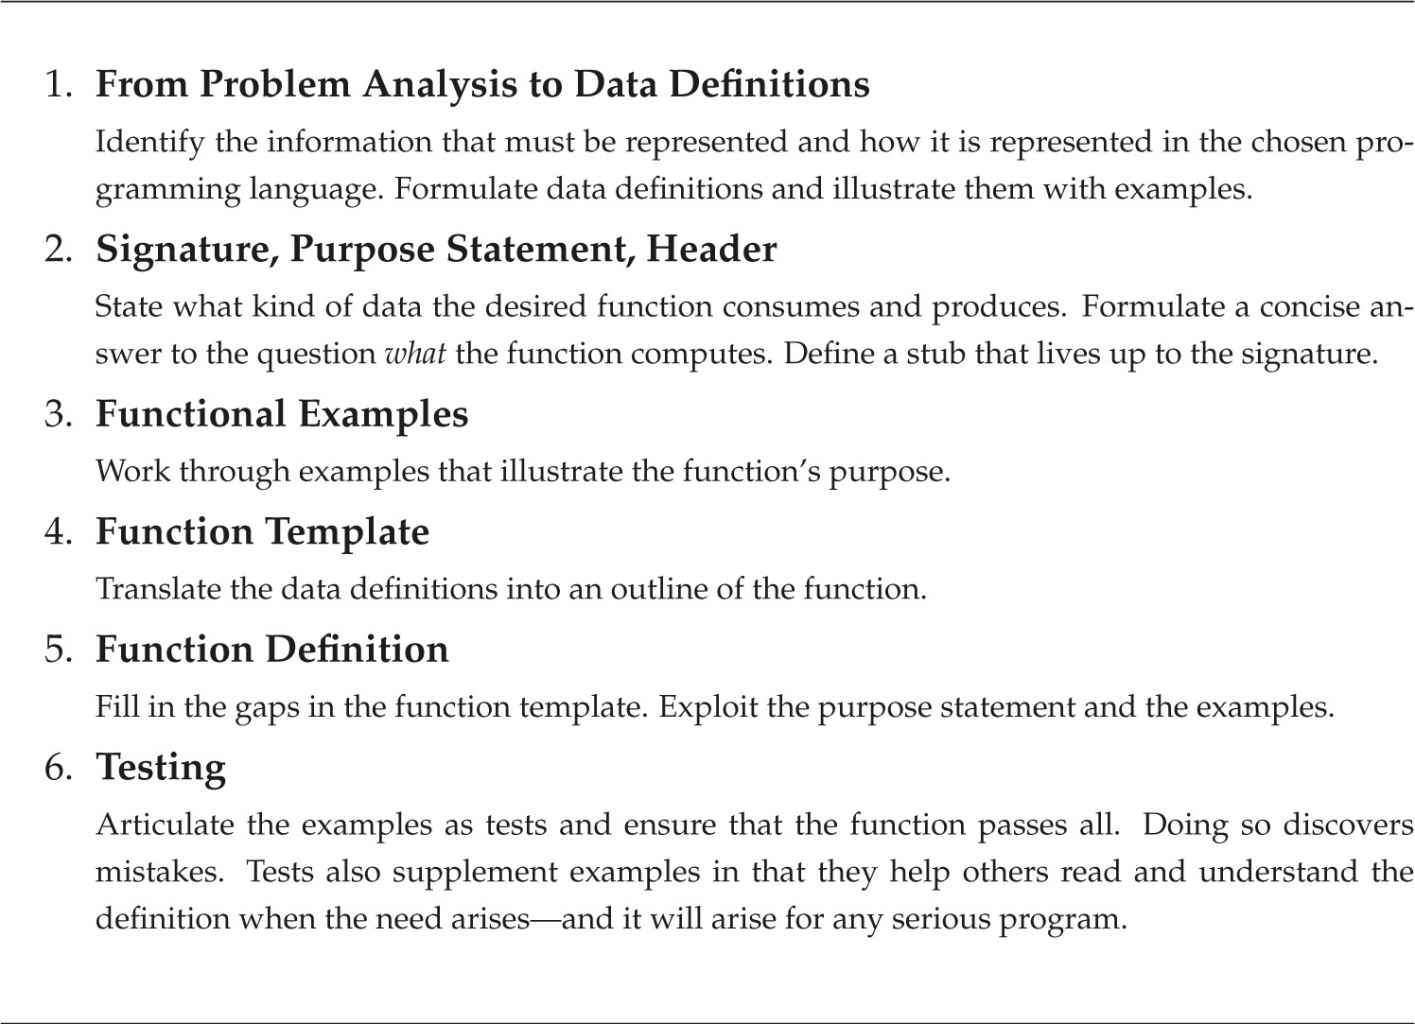
\includegraphics[width=0.88\textwidth]{images/00001.jpeg}
  \caption{函数设计配方的核心步骤}
  \label{fig:design_recipe_steps}
\end{figure}

\begin{notebox}[教师建议]
建议让学生将图~\ref{fig:design_recipe_steps} 的核心步骤抄写在索引卡片（卡片纸）的一面。当学生在解题中陷入困境不知所措时，让他们拿出卡片，并指出他们当前停滞在哪个步骤上。
\end{notebox}

设计流程的每一步都配有针对性极强的关键提问。对于某些步骤——例如构造功能示例或提炼函数模板——这些提问会直接依托于数据定义。回答这些问题几乎能够自然而然地生成中间产物。这种“脚手架”（scaffolding）机制在进入整个流程中唯一的创造性步骤——完成函数定义的编写时，将展现出巨大的威力。即便利在此时，在绝大多数情况下依然有规律可循、有法可依。

\begin{notebox}[教师建议]
在整个设计流程中，最为关键的问题集中在步骤~4 与步骤~5。建议让学生用他们自己的语言，将这两个步骤的核心问题抄写在索引卡片的背面。
\end{notebox}

这种方法的创新之处在于：它为初学者阶段的程序创建了明确的\term{中间产物}。当一个新手卡壳时，专家或导师可以通过审查现有的中间产物来诊断问题所在。导师通过抛出设计流程中的通用提问，引导新手进行自我审视并自主修正错误。这种\textbf{自我赋能}（self-empowering）的思维训练过程，正是单纯的随意编码与真正的程序设计之间的分水岭。

\term{逐步求精}（Iterative Refinement）旨在应对现实问题的复杂性与多面性。试图一蹴而就、一次性把所有细节都做对，几乎是不可能的。计算机科学家从物理科学中借鉴了逐步求精的思想来攻克这一设计难题。其本质思想是：首先剥离掉所有非本质的细枝末节，先为保留下来的核心问题找到一个清晰的解决方案。随后，在每一次求精步骤中，重新引入一个之前忽略的细节，并尽可能复用现有的解决方案来解决扩展后的新问题。重复（即迭代）这一求精过程，最终便能得到一个完备的解决方案。

从这个意义上说，程序员就像是一位“微型科学家”。科学家针对现实世界的某种理想化模型进行建模，以便对其做出预测。只要模型的预测与观测吻合，一切便顺利成章；一旦预测与实际观测出现偏差，科学家就会修正并提炼模型以缩小差距。同理，当程序员接到一项任务时，他们会完成初步设计，将其转化为代码，交由真实用户进行评估，随后通过持续的逐步求精，直至程序的行为与目标产品高度吻合。

本书通过两种不同的方式引入逐步求精。由于当程序结构变复杂时通过求精进行设计尤为关键，本书在第四部分随着问题难度的大幅提升，正式系统地引入了该技术。此外，在本书前三部分中，我们也通过在后续章节中针对同一问题提出越来越复杂的变体，潜移默化地运用逐步求精——即在一个章节中解决问题的核心，在后续章节中引入新概念的同时，为该问题增添相匹配的细节维度。


% ------------------------------------------------------------------------------
\section*{DrRacket 与教学语言}
\addcontentsline{toc}{section}{DrRacket 与教学语言}
\label{sec:preface:drracket_languages}
% ------------------------------------------------------------------------------

学习设计程序需要反复的亲身动手实践。正如不弹琴绝不可能成为钢琴家一样，不编写实际程序并让它们正确运行，任何人都不可能成为优秀的程序设计者。因此，本书配备了一套极简而精悍的软件支持环境：一门用于书写程序的编程语言，以及一个让读者能够像编辑文本一样编写程序并直接运行的集成开发环境。

许多我们在生活中遇到的人都说他们渴望学会写代码，接着便询问应该学习哪门编程语言。鉴于媒体对某些流行语言的大肆宣传，提出这样的问题并不令人意外，但这种问法从根本上就走入了误区。在当下时髦的某种流行语言中学习编程，往往是在为学生未来的挫败埋下伏笔。技术世界的流行风潮极其短暂。一本典型的“X 天精通某语言”的书籍或速成班，根本无法传授能够迁移到下一波潮流语言中的核心计算原理。更糟糕的是，工业级语言本身的繁杂语法与特殊机制，往往严重干扰了可迁移技能的吸收——无论是在表达解决方案的思维层面，还是在处理程序错误与调试的认知层面。

\begin{notebox}[教师建议]
对于非零基础受众或高阶课程，在教学中亦可直接使用工业界现成语言配合本设计配方进行讲授。
\end{notebox}

与此相反，学习设计程序的核心在于研习根本原理与获得可终身迁移的技能。理想的教学编程语言必须全心全意服务于这两个目标，然而市面上现存的任何工业语言都无法胜任。其致命瓶颈在于：初学者在尚未全面掌握语言语法之前就会犯错，而工业级语言的报错诊断机制却总是假定程序员已经通晓整门庞大的语言体系。结果就是，晦涩难懂的报错信息常常令初学者如坠云雾，大受打击。

我们的解决方案是：从我们专门量身定制的教学语言开始起步，这门语言被称为\term{初学学生语言}（Beginning Student Language，简称 \term{BSL}）。这门语言本质上就是学生在初等代数课程中所习得的“算术与代数符号系统”。它涵盖了函数定义、函数调用以及条件表达式的记法，并且支持表达式的任意嵌套。由于这门语言的规模极小，其报错诊断信息即使基于整门语言的规则给出，对于仅具备初等代数知识的读者而言依然一目了然、清晰易懂。

\begin{notebox}[教师建议]
教师可以向学生解释：BSL 本质上就是初等代数，只是在此基础上扩充了若干额外的数据类型（如字符串、布尔值、图像等），以及定义在这些数据之上的一系列内置函数。
\end{notebox}

一旦学生完全掌握了基于结构的程序设计原则，便可以进阶到\term{中级学生语言}（Intermediate Student Language，简称 \term{ISL}）以及更高阶的教学方言，统称为 \term{*SL}。本书利用这些进阶方言来传授抽象设计原则与通用递归算法。我们坚信，通过这一系列循序渐进的教学语言的淬炼，能够为读者未来在广泛的专业编程语言（如 JavaScript、Python、Ruby、Java 等）中构建高质量软件提供无可比拟的深厚底蕴。

\begin{notebox}[关于 Racket 的说明]
这套教学语言系列全部基于 Racket 实现——Racket 是我们专门为了“打造编程语言”而开发的一门现代编程语言。如今，Racket 已经走出象牙塔，在工业界的各类实际场景中大显身手，从游戏开发到射电望远镜阵列的运行控制皆有其身影。尽管教学语言从 Racket 中汲取了诸多语法与设计元素，但本书并不专门教授 Racket。当然，彻底学完本书的学生，完全可以轻而易举地过渡并熟练使用 Racket。
\end{notebox}

在编程环境的选择上，我们面临着与编程语言同样的困境。面向专业工程师的现代开发环境，其复杂程度堪比巨型客机的驾驶舱，密密麻麻的仪表盘与控件足以让任何初次启动该软件的新人感到窒息。初学程序员真正需要的，是一架双座单发螺旋桨式教练机，让他们能够全神贯注地操练基本飞行技能。为此，我们量身打造了 \term{DrRacket}——一个专为初学者设计的交互式集成开发环境。

DrRacket 凭借两个极其简洁的交互窗格，全力支持富有趣味性、反馈即时的探索式学习：位于上半部分的\term{定义区}（definitions area）用于编写函数与常量定义；位于下半部分的\term{交互区}（interactions area）则允许程序员即时求值并测试引用了这些定义的表达式。在这样的环境中，探索“如果……会怎样”（what-if）的假设场景就像在电子表格软件中那样轻松自如。从初次接触的第一分钟起，读者就可以从经典的计算器式操作开始实验，并迅速过渡到对图像、文本及各种丰富数据形态的动态计算。

像 DrRacket 这样的交互式开发环境在两个关键维度上极大地降低了学习门槛。首先，它让初学者能够直接操控真实数据。由于省去了从文件或外设中读取输入信息的繁杂代码，初学者不必将宝贵精力虚耗在理解底层 I/O 机制上。其次，这种布局在架构上严格地将“数据及其内部计算逻辑”与来自现实世界的“输入/输出展现”分离开来。在当今软件工程界，这种解耦思想被视为系统化软件设计的基石，并被赋予了闻名遐迩的名字：\term{模型-视图-控制器}（Model-View-Controller，简称 \term{MVC}）架构。通过在 DrRacket 中学习，初学者从起步的第一天起，便在潜移默化中自然吸收了这一现代软件工程的核心范式。


% ------------------------------------------------------------------------------
\section*{可以迁移的技能}
\addcontentsline{toc}{section}{可以迁移的技能}
\label{sec:preface:skills_transfer}
% ------------------------------------------------------------------------------

通过学习系统性程序设计所习得的技能，具有双向迁移的深远价值。首先，它们自然适用于广义上的所有通用编程任务，乃至针对电子表格、音乐合成器、网页样式表甚至是文字处理器的自动化开发。我们的长期教学观察表明，图~\ref{fig:design_recipe_steps} 所示的设计流程能够无缝迁移到几乎任何现代编程语言中，并且无论是编写 10 行的小函数，还是驾驭 10,000 行的大型软件模块，它都同样行之有效。要在跨越不同编程语言与不同规模问题时熟练运用该设计流程，确实需要一番反思与内化；然而一旦该流程化为你的第二天性，其所带来的巨大生产力与质量收益将在各个方面显现。

此外，学习设计程序还意味着掌握两种具有普适价值的核心素养。程序设计无疑能够传授与数学（尤其是代数与几何）相同的严谨分析能力。然而与传统数学不同的是，与程序打交道是一种高度主动、富于互动性的学习方式。编写软件能够给予即时的正反馈，从而激发持续的探索、实验与自我评估。最终的产物通常是生动交互的软件作品，与传统教科书中枯燥单调的死记硬背练习相比，这能极大地增强学生的成就感与自信心。

除了强化数学思维之外，程序设计还是一门关于\textbf{分析性阅读与精确写作}的绝佳训练。哪怕是最小的程序设计任务，最初都是以文字应用题（word problem）的形式呈现的。缺乏扎实的阅读理解与分析能力，就绝不可能设计出能够解决复杂现实问题的优质程序。反之，程序设计方法强制要求创作者必须用规范、精确的语言来清晰阐述其思考过程。事实上，如果学生真正领会了设计配方的精髓，他们在思维表达与条理性方面的提升将远超其他任何技能。

为了说明这一点，不妨重温图~\ref{fig:design_recipe_steps} 中总结的设计流程。它要求设计者必须按部就班地：
\begin{enumerate}
  \item 分析问题陈述（通常以文字应用题的形式给出）；
  \item 抽象地提取并精确表达其核心概念与本质；
  \item 用具体的典型示例来验证并具象化这种本质；
  \item 基于前述分析制定清晰的设计大纲与规划；
  \item 依据预期的目标输出对设计产物进行客观评估；
  \item 根据未通过的测试用例与逻辑检查对产物进行系统修正。
\end{enumerate}

每一步都需要严谨的分析、精确的描述、高度的专注以及对细节的一丝不苟。任何一位经验丰富的企业家、工程师、记者、律师或科学家，都会深切认同上述技能在其日常核心工作中是何等不可或缺。在纸面上和 DrRacket 中亲身实践程序设计，正是习得这些宝贵素养的一条充满乐趣与智力美感的途径。

同样，逐步求精的设计方法绝不仅限于计算机科学与软件构建。建筑师、作曲家、作家以及各领域的专业人士亦是如此行事。他们的创作始于脑海中的灵感火花，并通过某种媒介勾勒其核心轮廓。随后他们在稿纸上反复斟酌推敲，直至最终作品尽可能完美地映射出其最初的心智构想。在将构思落于纸面的过程中，他们所运用的技巧与我们完全内化的设计配方如出一辙：或是通过素描绘画，或是通过文字修辞，或是通过指尖琴键，来展现建筑的风骨、刻画人物的性格或编织动人的旋律。使他们在迭代开发过程中保持高效产出的秘诀在于：他们已经将基本的设计配方化为本能，并能在面对具体情境时精准挑选出最适宜的工具。


% ------------------------------------------------------------------------------
\section*{本书的结构与组成}
\addcontentsline{toc}{section}{本书的结构与组成}
\label{sec:preface:structure}
% ------------------------------------------------------------------------------

本书的宗旨是引领没有任何编程经验的初学者步入系统化程序设计的殿堂。与此并行，本书提出了一种关于计算的\term{符号视角}（symbolic view of computation），这是一种专门阐明“程序作用于数据时的内部运作机制”的心智模型。粗略地说，这种方法推广并升华了学生在小学算术与初中代数中所学的运算规则。不过读者大可放心，DrRacket 内置了一个强大的机制——\term{代数单步求值器}（algebraic stepper），它能够一步一脚印地将这些计算推导过程以直观可视的方式完整展现出来。

全书主体由六个大部分组成，各部分之间穿插了五个“插曲”（intermezzo），并由“序幕”（Prologue）与“尾声”（Epilogue）首尾呼应。各大主要部分专注于传授核心程序设计思维，而各个插曲则介绍与编程机制和计算理论相关的补充概念与工具。

\begin{itemize}
  \item \textbf{序幕（Prologue）}是对纯粹编程的一次快速领略。它向读者展示了如何在教学语言中编写一个简单的火箭降落动画。完成之后，任何初学者在感到大开眼界、信心倍增的同时，也难免会感到些许手足无措。因此，序幕末尾的要点总结阐述了为什么脱离设计的随意编码是不可取的，以及循序渐进的系统化设计方法如何消除每个初学者必然经历的畏难心理。至此，全书核心舞台正式拉开序幕：
  
  \item \textbf{第一部分：固定大小的数据（Part I）}借助简单明了的案例讲解系统性设计的最核心概念。其核心立论是：程序设计者通常对程序需要消费与生成什么样的数据有初步的理解；因此，系统化的设计方法必须从对流入和流出程序的数据描述中提取尽可能多的指导线索。为了由浅入深，本部分从原子数据（数字、图像等）起步，循序渐进地引入描述数据的各种新形态：区间、枚举、分类数据、结构体以及它们的复合结构。
  
  \item \textbf{插曲 1（Intermezzo 1）}详尽剖析初学学生语言（BSL）的底层全貌：词汇表、文法规则及其运行语义。计算机科学家将这些称为语法（syntax）与语义（semantics）。程序设计者借助这一严谨的计算模型，能够准确预测其代码在运行时的求值行为，并高效分析诊断运行错误。
  
  \item \textbf{第二部分：任意大小的数据（Part II）}在第一部分的基础上展开延伸，引入了表达能力最强、最为实用的数据形态：任意大小的复合数据（列表）。第一部分中嵌套数据结构的深度和广度在代码中是固定的；本部分展示了一种精妙的通用化推广，带领我们跨越到任意大小的数据世界，随后重点转向处理此类数据的系统化程序设计。
  
  \item \textbf{插曲 2（Intermezzo 2）}引入了一种用于书写大规模复杂数据的紧凑而强大的表达记法：引用（quotation）与反引用（anti-quotation）。
  
  \item \textbf{第三部分：抽象（Part III）}敏锐地指出第二部分中编写的许多函数在结构上高度相似。优秀的编程语言绝不应强迫程序员一遍遍撰写大同小异的代码；相反，优良的语言必将提供消除此类冗余相似性的利器。计算机科学家将消除相似性的步骤及其产物统称为\term{抽象}（abstraction），并深知抽象能够成倍提升程序员的生产力。因此，本部分全面系统地传授创建与使用高阶抽象的设计配方。
  
  \item \textbf{插曲 3（Intermezzo 3）}承担着双重任务。一方面，它深入阐释了\term{词法作用域}（lexical scope）这一核心概念——即编程语言如何将每个名称严格绑定到程序员能够通过静态审查代码找到的唯一对应定义；另一方面，它介绍了一个包含丰富抽象机制的实用库，包括现代语言中常见的 \code{for} 循环推导式。
  
  \item \textbf{第四部分：交织数据（Part IV）}对第二部分的数据形态进行了更宏大的推广，并正式将“逐步求精”这一核心思维范式纳入设计方法工具箱中。
  
  \item \textbf{插曲 4（Intermezzo 4）}通过直观生动的实例，解释了为什么在所有现代计算机编程语言中十进制浮点数的运作机制常常出人意料。每一位抱负远大的未来程序员都必须掌握这些关于底层数字表示的关键事实。
  
  \item \textbf{第五部分：生成型递归（Part V）}增添了一项崭新的设计原则。虽然结构化设计与抽象足以应对绝大多数日常编程任务，但面对某些棘手问题时，它们偶尔会导致程序性能不足——即结构化设计的函数可能需要耗费过多时间或算力才能得出最终答案。因此，计算机科学家会设计出巧妙依托问题领域专属洞察的算法（如快速排序或二分搜索）。本部分展示了如何系统化地设计这一大类经典的生成型算法。
  
  \item \textbf{插曲 5（Intermezzo 5）}借助第五部分的经典案例，生动展示了计算机科学家是如何严谨分析与思考算法性能（时间与空间开销）的。
  
  \item \textbf{第六部分：累加器（Part VI）}为设计者的工具箱增添了终极秘诀：\term{累加器}（accumulators）。通俗地说，累加器为函数引入了“上下文记忆”。引入记忆机制能够大幅提升前四部分中结构化设计函数的执行效率；而对于第五部分中的复杂算法，累加器往往是能否在有限时间内求出答案的决定性分水岭。
  
  \item \textbf{尾声（Epilogue）}对全书体系进行了全景式的总结评估，并为有志于继续攀登计算高峰的读者指明了进阶方向。
\end{itemize}

自学读者应当通读全书，从第一页按部就班地学至最后一页。我们之所以强调“切实操练”，是因为读者应当动手解答全书所有的练习题，或者至少确保自己彻底清楚如何解答它们。

同样，任课教师应尽可能多地覆盖全书内容，从序幕一直贯彻至尾声。根据我们数十年的教学经验，这在完整学期中是完全切实可行的。通常，我们会在学期课程中布置一个大型且趣味盎然的综合项目（例如一个完整的交互式电子游戏）。然而我们也充分理解，在特定教学学时限制下可能需要做出针对性裁剪，且不同教师的教学风格对本书的取舍亦有所不同。

图~\ref{fig:book_dependencies} 为希望灵活选读本书内容的读者提供了一份清晰的导航图。该图展示了各个部分与插曲之间的逻辑依赖关系。实线箭头表示严格的强依赖关系（例如学习第二部分必须先掌握第一部分）；虚线箭头则主要作为建议参考（例如跳过序幕并不会影响后续主体章节的学习）。

\begin{figure}[htbp]
  \centering
  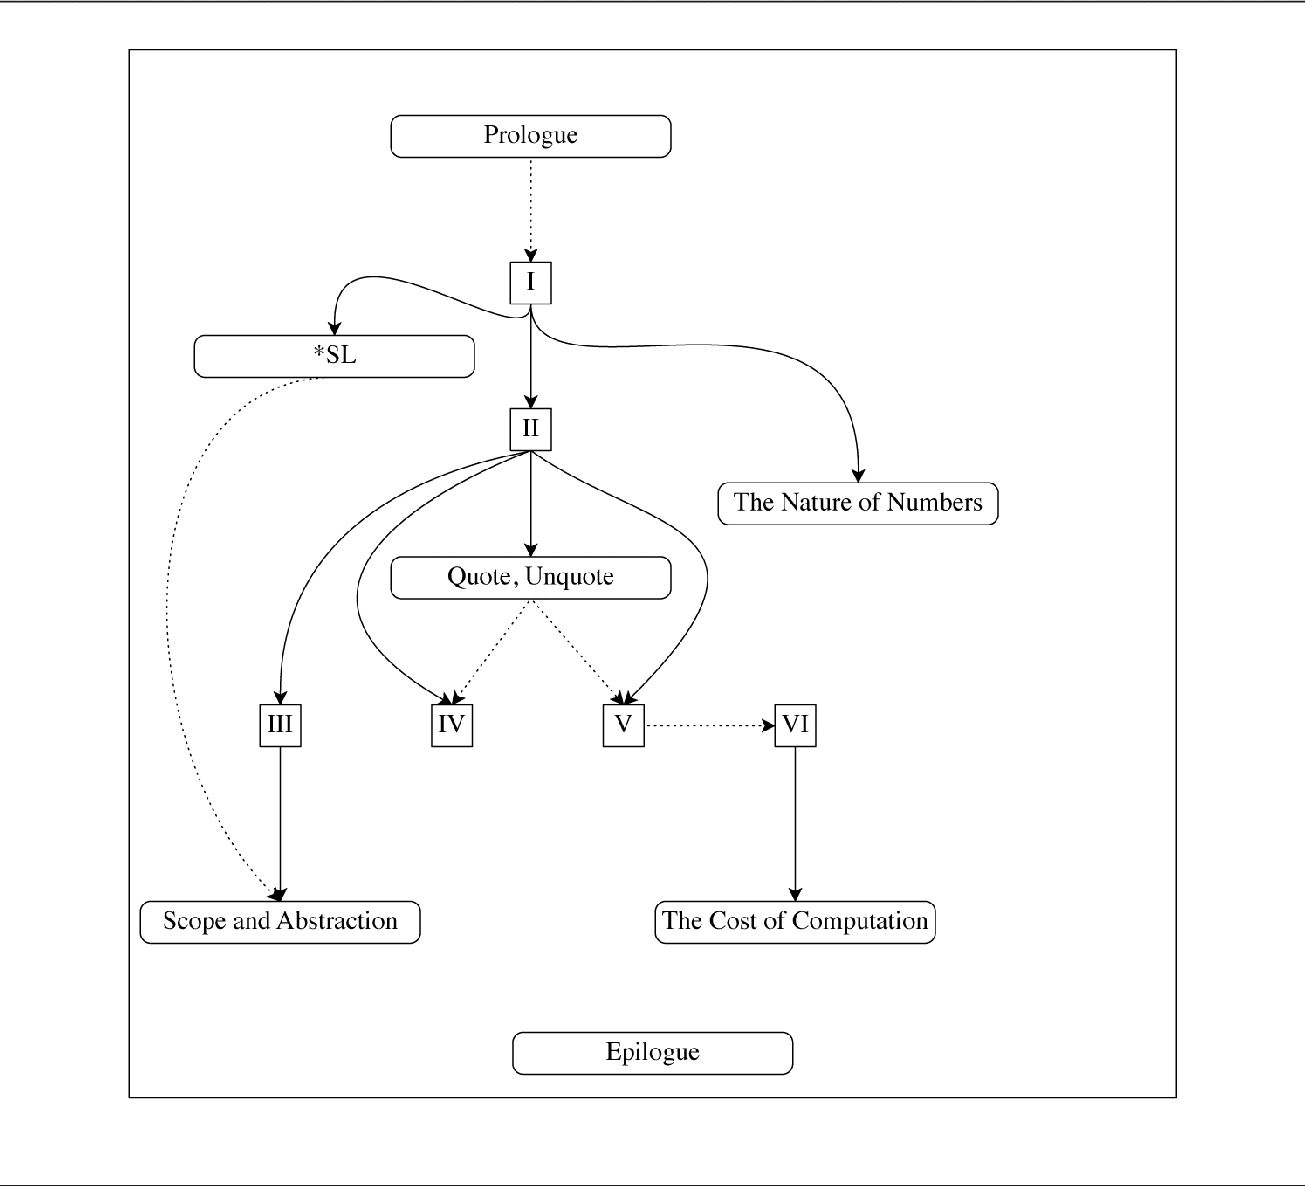
\includegraphics[width=0.88\textwidth]{images/00002.png}
  \caption{全书各部分与各插曲之间的依赖关系图}
  \label{fig:book_dependencies}
\end{figure}

基于该依赖图，我们为不同的教学场景推荐三种可行的学习路径：
\begin{itemize}
  \item \textbf{高中课程}：建议教师尽可能覆盖第一部分与第二部分，并在期末安排一个小型综合项目（如开发一款图形小游戏）。
  \item \textbf{大学学季制（Quarter）课程}：建议重点讲授第一部分、第二部分、第三部分与第五部分，并涵盖关于教学语言语义及词法作用域的插曲。
  \item \textbf{大学学期制（Semester）课程}：若希望尽早向学生揭示程序设计中的性能权衡，推荐在讲完第一和第二部分后，直接衔接第六部分中不依赖第五部分的累加器内容，随后讨论插曲~5，并在此视角下全面展开全书其他内容的教学。
\end{itemize}

\paragraph{螺旋式案例主题的持续迭代}
本书在全书各章节的例题与习题中反复回归若干经典主题。例如，“虚拟电子宠物”（virtual pets）贯穿了第一部分的始终，甚至在第二部分再度登场；又如，第一和第二部分分别从不同角度探讨了交互式文本编辑器的架构实现；图结构算法在第五部分登场后，立刻在第六部分中被再次深入剖析。这种反复回归同一主题的用意，在于从侧面潜移默化地引入并强化“逐步求精”的思想。我们强烈建议任课教师布置这些主题连续的系列习题，或结合自身教学特色设计类似的螺旋进阶习题序列。


% ------------------------------------------------------------------------------
\section*{两版之间的差异}
\addcontentsline{toc}{section}{两版之间的差异}
\label{sec:preface:differences}
% ------------------------------------------------------------------------------

《程序设计方法》第二版相较于第一版，在以下几个核心维度上做出了重大革新：

\begin{enumerate}
  \item \textbf{严格区分完整程序的设计与单个函数的设计}。具体而言，本版重点聚焦于两类典型程序架构：事件驱动程序（主要是图形用户界面 GUI 程序，也包括分布式网络程序）与批处理程序。
  
  \item \textbf{程序的构建明确划分为“自顶向下的规划阶段”与“自底向上的实现阶段”}。我们清晰地展示了外部库接口如何决定特定程序构件的代码形态。尤为突出的是，程序设计的最早阶段会直接产出一张\term{愿望清单}（wish list）。虽然愿望清单的概念在第一版中已初见端倪，但第二版将其确立为一项核心设计法则。
  
  \item \textbf{愿望清单中每个条目的落地实现，都严格遵循函数设计配方}，这构成了全书六大主体部分的核心内容。
  
  \item \textbf{结构化设计的一个决定性法则，是定义由若干子函数组合而成的复杂函数}。这种\term{组合式设计}（design-by-composition）在批处理程序的世界中尤为重要。与生成型递归相似，它需要灵光一闪的洞察力——即敏锐地意识到：由前一个函数生成中间数据结构、再由后一个函数对其进行处理，能够极大地简化整体设计。这种方法同样依赖愿望清单，但提出这些愿望需要针对中间数据定义进行富有远见的架构设计。第二版在书中精心穿插了大量针对组合式设计的专题训练。
  
  \begin{notebox}[致意]
  我们由衷感谢 Kathi Fisler 提醒我们重视组合式设计在现代教学中的关键地位。
  \end{notebox}
  
  \item \textbf{全面内置现代自动化测试支持}。虽然测试始终深植于我们的设计哲学之中，但教学语言与 DrRacket 直到 2002 年（第一版出版后不久）才从底层完备支持了自动化测试工具（如 \code{check-expect}）。新版彻底依托这套现代化的测试支持体系，使测试贯穿于教学的每一环节。
  
  \item \textbf{完全移除了命令式程序设计（imperative programming）的内容}。第一版的旧章节依然可以在线免费获取。这部分材料经过现代化重构后，将收录在本书的姊妹篇《How to Design Components》（如何设计组件）中。
  
  \item \textbf{全书案例与习题全面采用现代化的教学包（teachpacks）}。首选的引入方式是在代码中通过 \code{require} 显式导入，同时也完全兼容在 DrRacket 菜单中手动加载。
  
  \item \textbf{在若干专业术语与符号记号上进行了重要革新}：
  
  \begin{table}[htbp]
    \centering
    \small
    \begin{tabular}{ll}
      \hline
      \textbf{第二版（Second Edition）} & \textbf{第一版（First Edition）} \\
      \hline
      签名（\code{signature}） & 契约（\code{contract}） \\
      分类数据（\code{itemization}） & 联合（\code{union}） \\
      \code{'()} & \code{empty} \\
      \code{\#true} & \code{true} \\
      \code{\#false} & \code{false} \\
      \hline
    \end{tabular}
    \caption{第一版与第二版核心术语及记号对照表}
    \label{tab:edition_differences}
  \end{table}
  
  最后三项符号的更新，极大地优化了列表在引用（quotation）语法下的表达一致性与可读性。
\end{enumerate}


% ------------------------------------------------------------------------------
\section*{致谢}
\addcontentsline{toc}{section}{致谢}
\label{sec:preface:acknowledgments}
% ------------------------------------------------------------------------------

\subsection*{第一版致谢}

有四位先驱应当获得我们最崇高的谢意：Robert ``Corky'' Cartwright，他与第一作者共同开创了莱斯大学（Rice University）经典入门先导课程的雏形；Daniel P. Friedman，正是他在 1984 年力邀第一作者重写经典著作《The Little LISPer》（亦由 MIT Press 出版），从而点燃了整个项目的最初火种；John Clements，他亲手设计、实现并持续维护着 DrRacket 中不可或缺的代数单步求值器；以及 Paul Steckler，他始终忠实地为团队提供强有力的支持，为我们的编程工具链贡献良多。

本书的诞生还得益于众多亲朋好友与同行学者的鼎力相助，他们在各自的课堂中试用了早期讲义，并对草稿给出了详尽深入的宝贵意见。我们由衷感激他们的热情支持与耐心包容：Ian Barland、John Clements、Bruce Duba、Mike Ernst、Kathi Fisler、Daniel P. Friedman、John Greiner、G{\'e}raldine Morin、John Stone 以及 Valdemar Tamez。

莱斯大学 Comp 210 课程的数十届学子在教学中试用了本书的早期书稿，并从各个维度为本书的完善做出了贡献。此外，参加过我们 TeachScheme! 师资培训工作坊的众多骨干教师在自己的中小学课堂上积极践行了早期讲义，并慷慨反馈了大量的宝贵建议。作为这些热忱贡献者的杰出代表，我们特别鸣谢：Barbara Adler 女士、Stephen Bloch 博士、Karen Buras 女士、Jack Clay 先生、Richard Clemens 博士、Kyle Gillette 先生、Marvin Hernandez 先生、Michael Hunt 先生、Karen North 女士、Jamie Raymond 先生与 Robert Reid 先生。Christopher Felleisen 耐心地同他的父亲一起通读了本书前几个部分，为我们提供了来自年轻初学者的最直接洞见。Hrvoje Blazevic（当时在 ``LPG/C Harriette'' 轮船上担任船长）、犹他大学的 Joe Zachary 以及印第安纳大学的 Daniel P. Friedman 在本书第一版第一次印刷中指出了若干勘误，我们在此次修订中已全部修正。谨向所有人致以最诚挚的谢忱。

最后，Matthias 谨向 Helga 致以最深切的感激，感谢她多年来的无限包容，为一个总是在神游天外的丈夫与父亲营造了温暖的港湾。Robby 由衷感谢黄幸惠（Hsing-Huei Huang）的全心支持与由衷鼓励；没有她的陪伴，他将一事无成。Matthew 感谢袁雯（Wen Yuan）始终如一的温暖守候与悠扬持久的音乐陪伴。Shriram 深深感激 Kathi Fisler 的坚定支持、包容耐心与诙谐妙语，以及她全程深度参与到这一宏大项目中所付出的心血。

\subsection*{第二版致谢}

正如在 2001 年那样，我们怀着由衷的敬意感谢 John Clements 设计、验证、实现并维护了 DrRacket 的代数单步求值器。这项长跑他已经坚持了近二十年，单步求值器早已成为全书概念讲解与教学互动中无可替代的支柱级工具。

在过去数年间，多位学术界同仁研读了书稿的各个版本并提出了宝贵的改进意见。我们由衷感激与以下诸位学者富有启发性的思想交流与探讨：Kathi Fisler（伍斯特理工学院与布朗大学）、Gregor Kiczales（不列颠哥伦比亚大学）、Prabhakar Ragde（滑铁卢大学）以及 Norman Ramsey（塔夫茨大学）。

多年来，数以千计的教师参加了我们的各类师资培训工作坊，并反馈了海量的教学心得。其中，Dan Anderson、Stephen Bloch、Jack Clay、Nadeem Abdul Hamid 与 Viera Proulx 的贡献尤为卓著，在此我们特别向他们在第二版编写过程中所发挥的重要作用致以最诚挚的敬意。

Guillaume Marceau 在与 Kathi Fisler 及 Shriram 的紧密合作下，耗费数月心血对 DrRacket 的错误诊断提示机制进行了脱胎换骨式的深入研究与重构。我们对其卓越的工作致以崇高敬意。

Celeste Hollenbeck 堪称我们所遇过的最不可思议的审校读者。在彻底读懂行文之前，她从不知疲倦地反复推敲质疑；在一节内容尚未能完全支撑其核心论点、结构尚未严丝合缝、段落句子尚未浑然一体之前，她绝不轻言放行。对她所付出的超凡努力，我们谨致以最深厚的由衷谢意。

我们还要向以下诸位致谢，感谢他们对第二版各阶段草稿提出的中肯批评与建设性意见：Saad Bashir、Steven Belknap、Stephen Bloch、Joseph Bogart Tomas Cabrera、Estevo Castro、Stephen Chang、Jack Clay、Richard Cleis、John Clements、Mark Engelberg、Christopher Felleisen、Sebastian Felleisen、Vladimir Gaji{\'c}、Adrian German、Ryan Golbeck、Jane Griscti、Alberto E. F. Guerrero、Nadeem Abdul Hamid、Wayne Iba、Jordan Johnson、Marc Kaufmann、Gregor Kiczales、Eugene Kohlbecker、Jackson Lawler、Ben Lerner、Elena Machkasova、Jay Martin、Jay McCarthy、Ann E. Moskol、Paul Ojanen、Klaus Ostermann、Alanna Pasco、S. Pehlivanoglu、David Porter、Norman Ramsey、Ilnar Salimzianov、Brian Schack、Tubo Shi、Stephen Siegel、Kartik Singhal、Marc Smith、Dave Smylie、Vincent St-Amour、{\'E}ric Tanter、Sam Tobin-Hochstadt、Manuel del Valle、David Van Horn、Mitch Wand、Roelof Wobben 与 Andrew Zipperer。

htdp.org 网站上优雅清晰的在线排版布局出自 Matthew Butterick 之手，他专门为我们的在线文档量身设计了这套排版样式。

最后，我们由衷感谢麻省理工学院出版社（MIT Press）的资深编辑 Ada Brunstein 与 Marie Lufkin Lee，她们慷慨许可我们在互联网上公开打磨这第二版《How to Design Programs》。我们亦诚挚感谢 MIT 的 Christine Bridget Savage 与 Westchester Publishing Services 的 John Hoey 统筹全书最后的出版印制流程；John Donohue、Jennifer Robertson 以及 Mark Woodworth 在文稿文字编辑方面完成了令人赞叹的杰出工作。

% ==============================================================================
% 序幕：如何编程 (Prologue: How to Program)
% ==============================================================================

\chapter{序幕：如何编程}
\renewcommand{\thefigure}{0.\arabic{figure}}\setcounter{figure}{0}
\renewcommand{\thetable}{0.\arabic{table}}\setcounter{table}{0}
\label{sec:prologue}

\begin{center}
  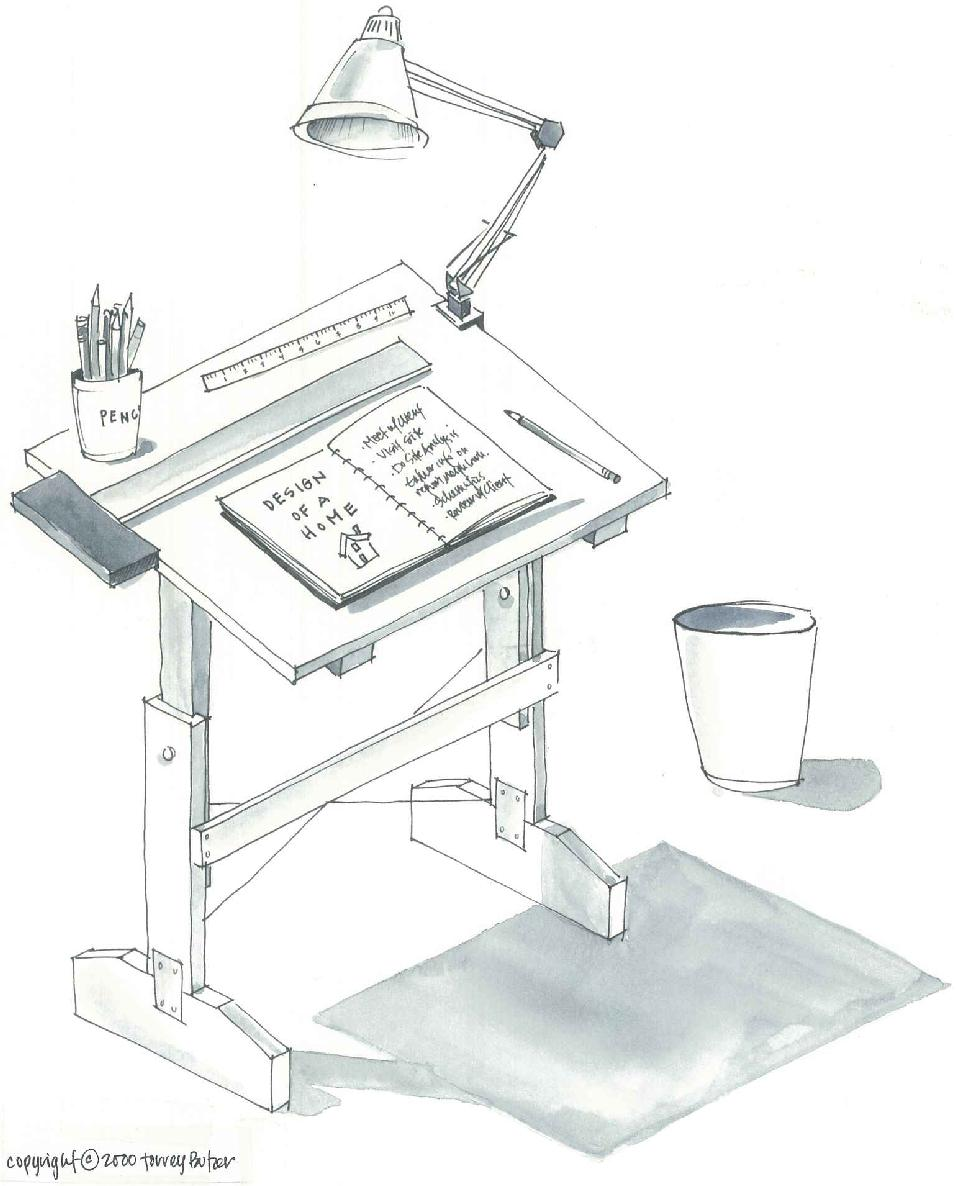
\includegraphics[width=0.45\textwidth]{images/00003.jpeg}
\end{center}

当你还是个幼童时，父母就教你数数，并用手指做简单的算术运算：“1 + 1 是 2”、“1 + 2 是 3”，等等。接着他们会问：“那 3 + 2 是几？”你会掰着一只手的手指头数出答案。他们负责下达指令（编程），你负责执行计算。从某种意义上说，这其实就是“编程”与“计算”的全部实质。

\begin{notebox}[环境准备]
从官方网站下载并安装最新版的 DrRacket 软件：\url{https://racket-lang.org}。
\end{notebox}

现在，是时候互换角色了。启动 DrRacket，你将看到如图~\ref{fig:meet_drracket} 所示的主界面。从顶部的“Language”（语言）菜单中选择“Choose Language...”（选择语言），在弹出的对话框中找到“How to Design Programs”分类下的“Teaching Languages”（教学语言），选择“Beginning Student”（初学学生语言，简称 \term{BSL}），然后点击“OK”完成设置。至此，角色彻底互换：你成为了发号施令的程序员，而 DrRacket 软件则成了那个乖巧听话、为你计算的小朋友。

让我们从最简单的计算开始。在 DrRacket 窗口的上半部分键入：
\begin{lstlisting}[language=BSL]
(+ 1 1)
\end{lstlisting}
点击右上角绿色的“Run”（运行）按钮，窗口的下半部分就会立即显示出一个醒目的结果：\code{2}。

\begin{figure}[htbp]
  \centering
  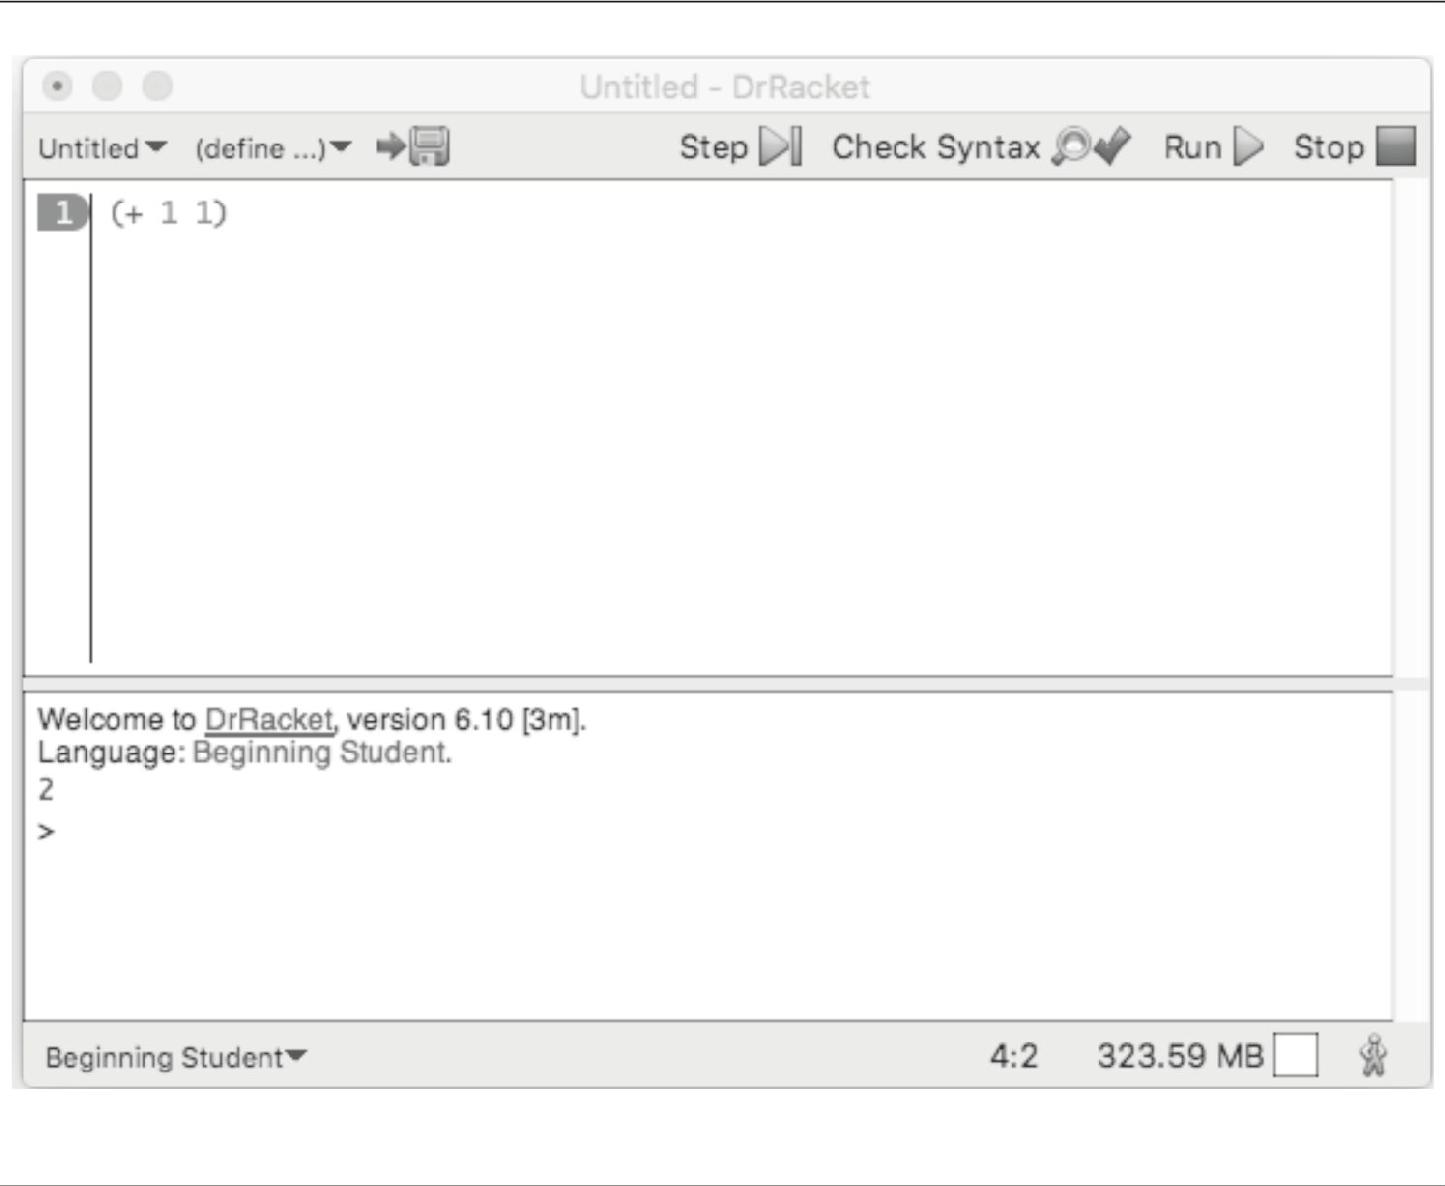
\includegraphics[width=0.9\textwidth]{images/00004.jpeg}
  \caption{初识 DrRacket 编程集成环境}
  \label{fig:meet_drracket}
\end{figure}

编程就是如此轻松直观。你像对待小朋友那样向 DrRacket 发问，DrRacket 为你完成计算。你也可以让 DrRacket 一次性处理多个运算请求：
\begin{lstlisting}[language=BSL]
(+ 2 2)
(* 3 3)
(- 4 2)
(/ 6 2)
\end{lstlisting}
点击“Run”后，DrRacket 的下半部分会依次输出：\code{4}、\code{9}、\code{2}、\code{3}，完全符合你的预期。

让我们放慢脚步，正式引入几个核心概念与专业术语：
\begin{itemize}
  \item DrRacket 窗口的上半部分称为\term{定义区}（definitions area）。在定义区中，你负责创建和修改程序代码，这一过程称为\term{编辑}（editing）。一旦你在定义区输入了字符或作出了任何修改，左上角就会亮起“Save”（保存）按钮。第一次点击“Save”时，DrRacket 会提示你输入文件名，以便将程序安全永久地保存在硬盘上。只要定义区与文件关联，点击“Save”就能确保你的全部心血安全留存。
  
  \item 程序由\term{表达式}（expressions）构成。在数学中你早已熟悉表达式的概念。在目前的 BSL 中，一个表达式要么是一个纯数字，要么是一个以左括号“\code{(}”开头、以匹配的右括号“\code{)}”结尾的括号结构——作为视觉奖励与辅助，DrRacket 会用阴影柔和地高亮配对括号之间的区域。
  
  \item 当你点击“Run”时，DrRacket 会自动对定义区中的所有表达式进行求值，并在下半部分的\term{交互区}（interactions area）中打印出求值结果。随后，DrRacket 作为忠诚的数字助手，在提示符（\code{>}）后静候你的下一步指示。提示符的出现表明 DrRacket 已经准备就绪，等待你在交互区直接输入额外的表达式并实时求值：
  \begin{replbox}
> (+ 1 1)
2
  \end{replbox}
\end{itemize}

在提示符后键入表达式，按下键盘上的回车键（Return / Enter），观察 DrRacket 给出的即时响应。你可以随心所欲地反复尝试：
\begin{replbox}
> (+ 2 2)
4
> (* 3 3)
9
> (- 4 2)
2
> (/ 6 2)
3
> (sqr 3)
9
> (expt 2 3)
8
> (sin 0)
0
> (cos pi)
#i-1.0
\end{replbox}

请格外仔细地观察最后一个结果。其前缀 \code{\#i} 是“我不大清楚绝对精确的值是多少，暂且用这个近似值代表”的缩写，在计算机科学中称为\term{不精确数}（inexact number）。与普通的袖珍计算器或其他编程系统不同，DrRacket 表现得极其诚实：当它无法给出完全精确的数学结果时，便会主动加上这个特殊前缀发出明确警示。在后续的插曲中，我们将为你揭开关于“计算机数字表示”的种种惊人真相，届时你定会由衷赞赏 DrRacket 的诚实与严谨。

此时你可能会好奇，DrRacket 能否一次性将两个以上的数字相加？答案是完全可以，而且有两种不同的写法：
\begin{replbox}
> (+ 2 (+ 3 4))
9
> (+ 2 3 4)
9
\end{replbox}
第一种写法是我们在学校代数课中所熟悉的\textbf{嵌套算术}（nested arithmetic）。第二种写法则是 BSL 原生的\textbf{前缀算术}。后者极为自然，因为在这种记法中，括号始终用来明确地将“运算操作符”与其“操作数”紧密组合在一起。

\begin{notebox}[关于 Racket 的说明]
尽管这个编辑器名为 DrRacket，但本书并不教授 Racket 语言本身。关于为何专为教学研发一套独立的教学语言体系，详见前言中关于教学语言的阐述。
\end{notebox}

在 BSL 中，每次想要执行计算操作时，你先写一个左括号，写下想要执行的操作符（例如 \code{+}），接着写下该操作所作用的各个数值（彼此用空格或换行分隔），最后以一个闭合的右括号结尾。紧跟在操作符后面的项称为\term{操作数}（operands）。所谓嵌套算术，意味着操作数本身也可以是一个表达式，因此：
\begin{replbox}
> (+ 2 (+ 3 4))
9
\end{replbox}
是一个完全合法的优良程序。你可以根据需要任意嵌套：
\begin{replbox}
> (+ 2 (+ (* 3 3) 4))
15
> (+ 2 (+ (* 3 (/ 12 4)) 4))
15
> (+ (* 5 5) (+ (* 3 (/ 12 4)) 4))
38
\end{replbox}
嵌套层数没有任何人为限制，唯一的限制是你的耐心。

自然，当 DrRacket 为你进行计算时，遵循的是你在数学中所熟知且钟爱的经典求值法则：只有当所有操作数都已化简为纯数字时，它才能算出加法的结果。如果某个操作数本身是一个带括号的子表达式，它会优先计算该内层表达式的值。与人类做四则运算不同，DrRacket 永远不需要为“先乘除还是先加减”这类运算符优先级伤脑筋——因为“自内向外”的纯括号求值是这里唯一通行的法则。

这种便利的代价是：\textbf{括号具有严格的语法意义}。你必须输入所有必需的括号，但绝不能输入多余的括号。例如在数学作业中添加多余的外层括号老师通常不会扣分，但在 BSL 中则绝对行不通。\code{(+ (1) (2))} 包含了多余的括号，DrRacket 会毫不客气地给出错误诊断：
\begin{replbox}
> (+ (1) (2))
function call: expected a function after the open parenthesis, found a number
\end{replbox}
不过一旦你习惯了 BSL 编程，就会发现这根本不是什么负担，反而带来了巨大的优势：首先，你可以对任意多个操作数同时施加操作：
\begin{replbox}
> (+ 1 2 3 4 5 6 7 8 9 0)
45
> (* 1 2 3 4 5 6 7 8 9 0)
0
\end{replbox}
如果你不确定某个操作符是否支持多个操作数，只需在交互区输入一个例子并敲击回车；DrRacket 会立刻告诉你它是否可行。或者按下 F1 打开 HelpDesk 查阅文档。其次，在阅读他人编写的程序时，你永远不需要费神去猜想哪个子表达式会优先被求值——清晰的括号与嵌套层次能够瞬间把求值顺序一览无遗地呈现在眼前。

\begin{notebox}[提示]
在在线版教材中，所有操作符的名称都超链接到了 HelpDesk 文档；在 DrRacket 中按 F1 亦可随时查看光标所在词的文档。
\end{notebox}

在此语境下，\term{编程}（programming）就是编写出易于理解的算术表达式，而\term{计算}（computing）就是求出表达式的值。借助 DrRacket，探索这种纯粹的编程与计算变得无比轻松。


% ------------------------------------------------------------------------------
\section{算术与“算术”}
\label{sec:prologue:arithmetic}
% ------------------------------------------------------------------------------

如果编程仅仅局限于枯燥的数字与四则运算，那它未免会像纯粹的初等数学那样单调。所幸的是，编程的世界远比数字丰富得多：文字、真假逻辑、图像以及更多丰富多彩的数据形态。

\begin{notebox}[幽默旁白]
开个玩笑：数学其实是一门极其迷人的学科，只是在当前的编程入门阶段，你并不需要用到高深的数学知识。
\end{notebox}

首先你需要了解的是，在 BSL 中，\term{文本}（text）是由双引号（\code{"}）括起来的任意键盘字符序列。我们将其称为\term{字符串}（string）。因此，\code{"hello world"} 是一个完全合法的字符串；当 DrRacket 对该字符串求值时，它就像对待数字那样，原封不动地在交互区将其回显出来：
\begin{replbox}
> "hello world"
"hello world"
\end{replbox}
事实上，许多程序员人生中写出的第一个程序，就是用来显示这行著名的问候语。

不仅如此，除了针对数字的算术之外，DrRacket 还精通针对字符串的“算术”。以下两个交互示例展示了这种独特的字符串算术：
\begin{replbox}
> (string-append "hello" "world")
"helloworld"
> (string-append "hello " "world")
"hello world"
\end{replbox}
正如 \code{+} 一样，\code{string-append} 也是一个操作符；它通过将后一个字符串拼接到前一个字符串的末尾来生成一个新字符串。正如第一个交互所示，这种拼接是完全原样的，两个字符串之间绝不会自动插入任何空格或标点。因此，如果你想要得到 \code{"hello world"}，就必须在其中一个单词中显式包含空格；这正是第二个交互所呈现的。当然，从两个单词构造该短语最自然的写法是：
\begin{replbox}
> (string-append "hello" " " "world")
"hello world"
\end{replbox}
因为与 \code{+} 一样，\code{string-append} 也能够同时接收任意多个操作数。

对字符串能做的事情远不止拼接。你可以从字符串中截取子串、翻转字符串、将所有字母转换为大写（或小写）、剔除两端的空格等等。最美妙的是，你根本不需要死记硬背这些函数名。只要在 HelpDesk 中检索相关词条，随时都能查到字符串支持的所有操作。

\begin{notebox}[使用 HelpDesk]
在键盘上按下 F1 键或使用顶部的帮助菜单打开 HelpDesk。阅读 BSL 手册中关于预定义操作的章节，特别是针对字符串的丰富操作函数。
\end{notebox}

如果你查阅了 BSL 的内置原语操作，会发现原语操作不仅能够消费字符串，还能生成数字：
\begin{replbox}
> (+ (string-length "hello world") 20)
31
> (number->string 42)
"42"
\end{replbox}
同时，也存在将字符串转换为数字的逆向操作：
\begin{replbox}
> (string->number "42")
42
\end{replbox}
如果你期待输入 \code{"forty-two"} 能得到 42，那可就想多了——这可不是一个严谨的字符串转换函数所能胜任的。

最后一个表达式引发了一个有趣的问题：如果有人将一个内部根本不是数字的字符串传给 \code{string->number}，会发生什么？在这种情况下，该操作会返回一种完全不同形态的结果：
\begin{replbox}
> (string->number "hello world")
#false
\end{replbox}
这既不是数字，也不是字符串，而是一个\term{布尔值}（Boolean）。与无穷无尽的数字和字符串不同，布尔值在全宇宙中只有两种可能取值：\code{\#true} 与 \code{\#false}。前者代表“真”，后者代表“假”。尽管取值只有两个，DrRacket 依然提供了一组专门用于组合布尔值的丰富操作符：
\begin{replbox}
> (and #true #true)
#true
> (and #true #false)
#false
> (or #true #false)
#true
> (or #false #false)
#false
> (not #false)
#true
\end{replbox}
运算结果完全符合操作符名称所传达的逻辑真意。（如果不熟悉 \code{and}、\code{or} 与 \code{not} 的逻辑法则，其实很简单：\code{(and x y)} 当且仅当 \code{x} 与 \code{y} 均为真时才为真；\code{(or x y)} 只要两者中至少有一个为真即为真；而 \code{(not x)} 在 \code{x} 为假时返回真，反之亦然。）

将两个数字进行对比并“转换”为一个布尔值也极其普遍：
\begin{replbox}
> (> 10 9)
#true
> (< -1 0)
#true
> (= 42 9)
#false
\end{replbox}

\begin{notebox}[停下来动手试一试]
请在交互区立即尝试以下三个表达式：\code{(>= 10 10)}、\code{(<= -1 0)} 以及 \code{(string=? "design" "tinker")}。最后一个表达式与前面略有不同，但别担心，你一定能轻松看懂它的含义。
\end{notebox}

伴随着所有这些新鲜的数据类型（没错，数字、字符串与布尔值都是数据）以及眼花缭乱的操作符，我们很容易遗忘之前学过的基本法则，比如嵌套算术：

\begin{lstlisting}[language=BSL]
(and (or (= (string-length "hello world")
            (string->number "11"))
         (string=? "hello world" "good morning"))
     (>= (+ (string-length "hello world") 60) 80))
\end{lstlisting}

这个表达式的求值结果是什么？你是如何推导出来的？是完全凭自己的心算，还是仅仅在 DrRacket 交互区中输入并按下了回车键？如果你是靠后者，你觉得脱离了电脑你自己能搞定吗？毕竟，如果你无法准确预测 DrRacket 对小型表达式的行为，当提交更庞大的程序时，你又怎敢轻易信赖它的运行结果呢？

在向你展示如何编写“真正”的程序之前，让我们再讨论一种更具趣味性的全新数据形态：\term{图像}（images）。当你在交互区中直接插入一张图片并按下回车时，如图：

\begin{stepperbox}
\begin{Verbatim}[commandchars=\\\{\}, fontsize=\footnotesize]
> \inlinesprite[1.4em]{images/sprites/rocket.png}
\end{Verbatim}
\end{stepperbox}

DrRacket 会原样回显这张图片！与其他许多编程语言截然不同，BSL 天生理解图像，并且支持针对图像的完整“图像算术”，就像它支持数字算术或字符串算术一样。简而言之，你的程序可以直接用图像进行加减组合等数学计算，而且在交互区就能即时演算。此外，BSL 程序员——正如其他语言的程序员一样——会编写出他人可以直接复用的代码库。使用这些库就像用新词汇扩充你的日常词典，或者用新原语扩充你的编程武器库一样自然。我们将这些专门用于辅助教学的库亲切地称为\term{教学包}（teachpacks）。

\begin{notebox}[在 DrRacket 中插入图片]
要在 DrRacket 中插入像小火箭这样的图片，可以使用顶部的“Insert”（插入）菜单中的“Insert Image...”（插入图像）。或者直接从网页浏览器中复制图片，粘贴到 DrRacket 的编辑窗格中。
\end{notebox}

一个极其重要的核心库是 \code{2htdp/image} 图像教学包，它支持测量图像宽度与高度的原语操作：

\begin{stepperbox}
\begin{Verbatim}[commandchars=\\\{\}, fontsize=\footnotesize]
(* (image-width \inlinesprite[1.4em]{images/sprites/rocket.png}) (image-height \inlinesprite[1.4em]{images/sprites/rocket.png}))
\end{Verbatim}
\end{stepperbox}

一旦在程序中引入了该库，点击“Run”就会得到 \code{1176}，因为这正是一张 28 像素宽、42 像素高的小火箭图像的面积。

\begin{notebox}[引入图像教学包]
在定义区顶部添加 \code{(require 2htdp/image)}，或者在“Language”菜单中点击“Add Teachpack...”，然后从预安装的 HtDP/2e 教学包菜单中选择 \code{image}。
\end{notebox}

你完全不需要打开搜索引擎去下载现成图片再插入程序中，你完全可以直接命令 DrRacket 从零绘制出基本的几何图形：

\begin{center}
  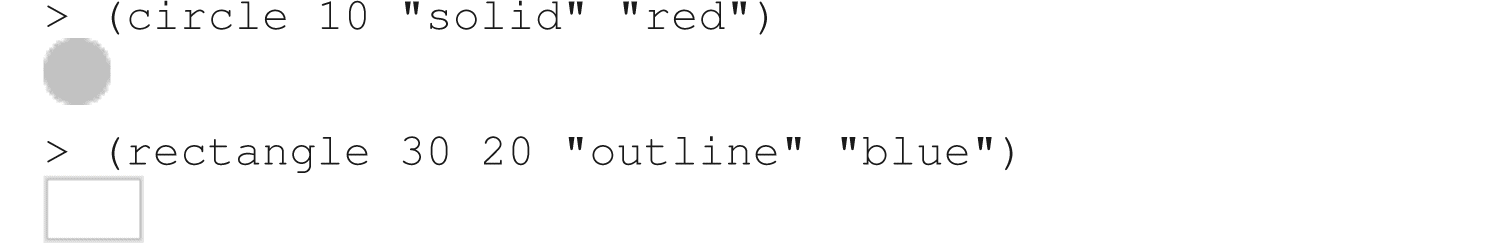
\includegraphics[width=0.85\textwidth]{images/00008.png}
\end{center}

当表达式的求值结果是一张图像时，DrRacket 会直接将其绘制在交互区中。而在程序内部，BSL 将图像视作与数字同等地位的数据。特别地，BSL 拥有用于组合图像的原语操作，正如用加号合并数字、用 \code{string-append} 拼接字符串一样自然：

\begin{center}
  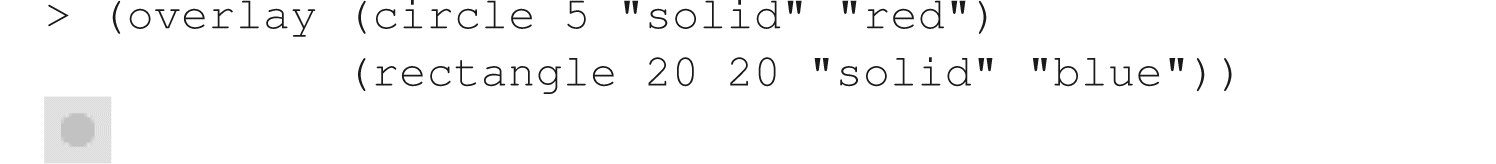
\includegraphics[width=0.85\textwidth]{images/00009.png}
\end{center}

如果将这两个图像按照相反的顺序叠放（将大正方形放在上面），则会得到一个纯蓝色的方块：

\begin{center}
  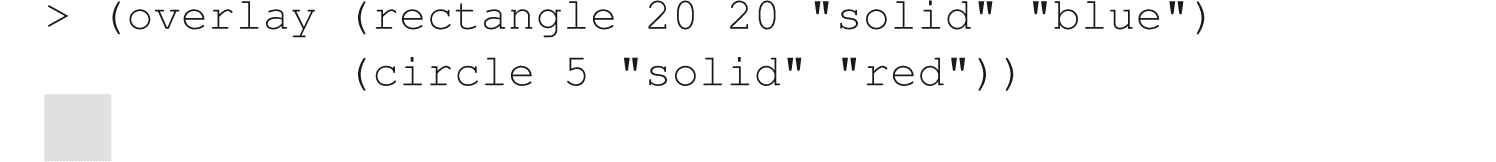
\includegraphics[width=0.85\textwidth]{images/00010.png}
\end{center}

停下来，思考一下为什么最后一个操作会盖住圆盘。

正如你所见，\code{overlay}（重叠）在感觉上比 \code{+} 更接近 \code{string-append}，但它确实是在“相加”图像，正如字符串拼接相加文本、加法操作相加数值一样。以下是关于这一思想的另一个例证：

\begin{replbox}
> (image-width (square 10 "solid" "red"))
10
> (image-width
    (overlay (rectangle 20 20 "solid" "blue")
             (circle 5 "solid" "red")))
20
\end{replbox}

上述与 DrRacket 的交互根本没有绘制任何画面，它们实际上只是在精确度量组合图像的宽度。

最后两个关键操作是 \code{empty-scene}（空场景）与 \code{place-image}（放置图像）。前者用于创建一个被称为\term{场景}（scene）的特殊矩形画布；后者则负责将指定图像精确放置到该场景中：

\begin{lstlisting}[language=BSL]
(place-image (circle 5 "solid" "green")
             50 80
             (empty-scene 100 100))
\end{lstlisting}

你将获得如下画面：

\begin{center}
  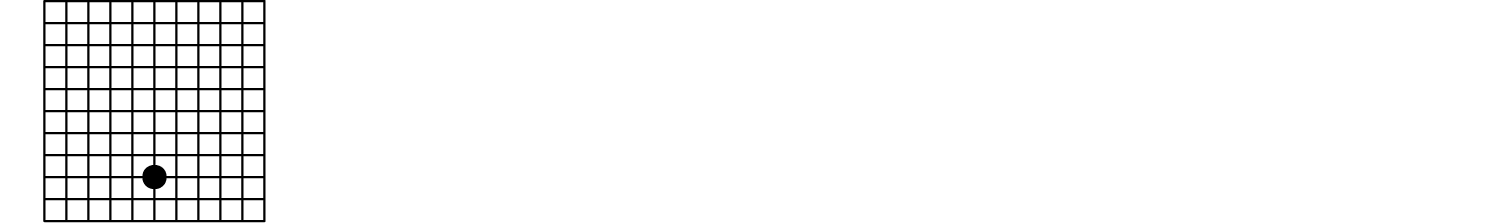
\includegraphics[width=0.35\textwidth]{images/00013.png}
\end{center}

\begin{notebox}[坐标系说明]
生成的真实场景中并没有参考网格线。我们在场景上叠加了坐标网格，以便你能清晰看到绿色圆点具体落在了何处。
\end{notebox}

从这幅图中可以看出，场景的坐标原点 \code{(0,0)} 位于窗口的\textbf{左上角}。与传统的笛卡尔数学坐标系不同，计算机屏幕上的 $y$ 坐标是\textbf{向下}递增的，而非向上。除此之外，画面完全符合预期：在宽 100、高 100 的空白矩形场景中，坐标 \code{(50, 80)} 处清晰地呈现着一个实心绿色圆盘。

让我们再次总结核心心智模型：所谓编程，就是书写清晰的算术表达式，但你的视野绝不再局限于单调的数字。在 BSL 中，算术是囊括了数字、字符串、布尔值乃至丰富图像的宏大算术体系。而计算，依然意味着求出表达式的最终值——只不过这个值可以是一个数字、一段文本、一个真假布尔值，或者一幅绚丽的图像。

现在，你已经彻底做好准备，编写能让小火箭在星空中飞翔的动态程序了！


% ------------------------------------------------------------------------------
\section{输入与输出}
\label{sec:prologue:inputs_output}
% ------------------------------------------------------------------------------

到目前为止，你所写的程序其实还相当局限。写下一行或几行表达式，点击“Run”，看到一些结果；如果再次点击“Run”，看到的依然是分毫不差的相同结果。事实上，无论你点击多少次“Run”，结果永远固定不变。简而言之，你的程序目前不过就像一台功能高级的掌上计算器，只是 DrRacket 能够计算包括图像在内的各种数据而已。

这既是一个好消息，也是一个坏消息。好消息在于：编程与计算本来就应当是计算器运算的自然推广。坏消息在于：编写软件的真正目的，在于用一套相同的计算逻辑去处理海量各异的数据，并动态产生形形色色的不同结果（而且计算速度应当远超人类手工）。也就是说，在掌握真正的编程之道前，我们还需要掌握更强大的工具。不过完全不必担心：凭借你对数字、字符串、布尔值与图像算术的扎实理解，你距离编写一个能够生成连续动画甚至电影的大作仅有一步之遥，绝非只是输出一句幼稚的“hello world”。这正是我们接下来的目标。

动画或电影本质上就是以极高频率按顺序快速连续放映的一组画面序列。如果你的代数老师当年知晓我们在上一节看到的“图像算术”，你们当年在代数课堂上完全可以制作精彩的电影，而不是计算枯燥的数字序列。不妨重温中学代数中常见的这种表格：

\begin{center}
\small
\setlength{\tabcolsep}{3.5pt}
\begin{tabular}{lcccccccccc}
  $x =$ & 1 & 2 & 3 & 4 & 5 & 6 & 7 & 8 & 9 & 10 \\
  \hline
  $y =$ & 1 & 4 & 9 & 16 & 25 & 36 & 49 & 64 & 81 & ?
\end{tabular}
\end{center}

代数老师通常会要求你在表格空白处填空，即用正确的数字替换问号“\code{?}”。

事实证明，制作动画丝毫不比完成这样一张数字表格复杂。事实上，动画的本质完全基于这种对照表格：

\begin{center}
  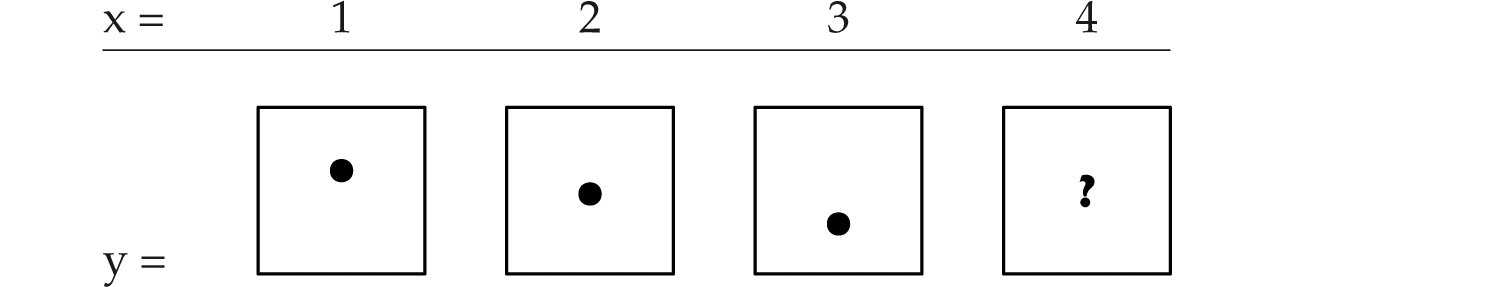
\includegraphics[width=0.85\textwidth]{images/00015.png}
\end{center}

具体来说，老师在这里会要求你画出第四个、第五个乃至第 1273 个画面，因为电影就是大量连续画面的集合（通常每秒需要 24 到 30 幅画面）。要制作一分钟的动画，大约需要 1200 到 1800 幅画面。

你也许还记得，代数老师不仅要求你计算序列中的第四或第五个数值，还会要求你写出一个通用的数学表达式，能够根据任意给定的输入 $x$ 计算出对应的输出 $y$。在纯数字的例子中，老师期待看到的答案通常是这样的：

\[
  y = x \cdot x
\]

只要将 1、2、3 等代入 $x$，便能依次求出对应的 $y$ 为 1、4、9 等——正如表格所记录的那样。而对于图像序列，你可以将其表述为：
\begin{quote}
$y =$ 包含一个距离场景顶部 $x^2$ 像素的圆点的画面。
\end{quote}
核心要点在于：这些能够统摄全局的规律单行式，已经不再是静态的表达式，而是\term{函数}（functions）！

乍看之下，函数长得很像表达式：左边总是一个 $y$，中间是一个等号，右边是一个算式。然而，它们绝非单纯的表达式。学校里关于函数的传统记法往往极具误导性。因此在 DrRacket 中，我们采用更清晰明确的记法来书写函数：
\begin{lstlisting}[language=BSL]
(define (y x) (* x x))
\end{lstlisting}

这里的关键字 \code{define} 表示“将 \code{y} 定义为一个函数”，它与表达式类似，用于计算出一个值。然而，函数的值取决于被称为\term{输入}（input）的动态值，我们通过 \code{(y x)} 来声明这一点。由于在定义函数时尚不知道具体输入是多少，我们使用一个名字来代表未知的输入。遵循代数传统，我们在这里用 \code{x} 代表未知的输入；不过很快，我们就会使用更具描述性的各种有意义的名称。

第二部分表明，你必须为 \code{x} 提供一个具体的数值，才能计算出 \code{y} 的具体结果。当你提供该数值时，DrRacket 会将该数值代入函数关联的主体表达式中。在这里主体表达式是 \code{(* x x)}。一旦 \code{x} 被具体数值（例如 1）替换，DrRacket 就能算出表达式的结果，该结果被称为函数的\term{输出}（output）。

\begin{notebox}[数学记法对比]
数学中常将 $y(1)$ 称为一次“函数应用”（function application），只是很多老师在课堂上忽略了向大家强调这个术语。
\end{notebox}

点击“Run”，你会发现什么动静都没有。交互区既没有打印任何结果，DrRacket 界面其他地方似乎也没有任何变化。你可能会觉得自己仿佛什么都没做成。但实际上你完成了一件大事：你成功定义了一个函数，并向 DrRacket 正式通告了它的存在！DrRacket 现在已经完全准备好供你随时调用该函数了。在交互区的提示符后输入：
\begin{replbox}
> (y 1)
1
\end{replbox}
这里的 \code{(y 1)} 在 DrRacket 中被称为一次\term{函数应用}（function application）或函数调用。再尝试：
\begin{replbox}
> (y 2)
4
\end{replbox}
便能看到 4 跃然眼前。当然，你也可以把这些测试调用全部写在定义区中，然后点击“Run”：
\begin{lstlisting}[language=BSL]
(define (y x) (* x x))
(y 1)
(y 2)
(y 3)
(y 4)
(y 5)
\end{lstlisting}
DrRacket 会在交互区依次输出：\code{1 4 9 16 25}，精准对应表格中的全部数值。现在，试着算出刚才表格中遗漏的第 1273 个数值吧！

这一切对于你而言意味着：函数提供了一种极其经济而强大的机制，只需一个统一的表达式，便能计算出无穷无尽的有趣结果。事实上，\textbf{程序本质上就是函数}；一旦透彻理解了函数，你就掌握了关于编程几乎所有核心奥秘的大门钥匙。鉴于其至高无上的地位，让我们系统梳理迄今为止关于函数的全部知识：
\begin{itemize}
  \item 首先，\code{(define (FunctionName InputName) BodyExpression)} 是\textbf{函数定义}。你能通过开头的 \code{define} 关键字瞬间认出它。它本质上由三部分构成：两个名称和一个表达式。第一个名称是函数本身的名称（\code{FunctionName}），你需要它来随心所欲地多次调用该函数；第二个名称被称为\term{形参}（parameter，即 \code{InputName}），代表在具体调用发生前未知的输入数据；最后的主体表达式（\code{BodyExpression}，称为\term{函数体}）负责根据具体输入计算出函数的输出。
  
  \item 其次，\code{(FunctionName ArgumentExpression)} 是\textbf{函数应用}（函数调用）。第一项指明你想要调用哪个函数；第二项则是作为输入传给该函数的具体实参表达式（\code{ArgumentExpression}）。如果是读桌面软件的说明书，可能会说该表达式“启动”了名为 \code{FunctionName} 的“应用程序”，并将 \code{ArgumentExpression} 作为输入传递给它。与所有表达式一样，实参可以是一个纯数据常量，也可以是一个深度嵌套的复杂子表达式。
\end{itemize}

函数的输入绝不仅限于数字，它们的输出也可以是任何丰富的数据形态。我们接下来的目标是创建一个能够模拟第二个表格（小圆点逐帧降落的场景图像序列）的函数，正如刚才的函数模拟了纯数字表格一样。由于利用表达式生成图像在中学阶段并未普及，让我们从最直观的步骤开始操练。还记得上一节末尾提到的 \code{empty-scene} 吗？在交互区输入：

\begin{center}
  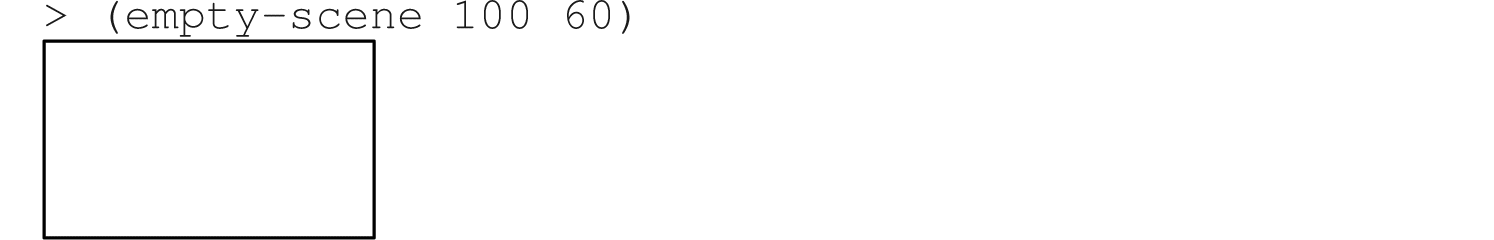
\includegraphics[width=0.85\textwidth]{images/00017.png}
\end{center}

DrRacket 会立即生成一个空白的矩形场景。我们可以利用 \code{place-image} 向该场景中置入图像：

\begin{center}
  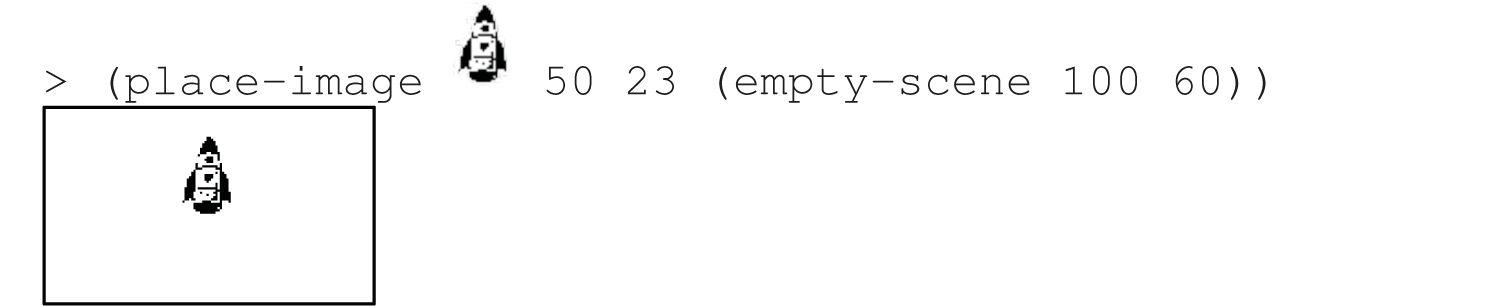
\includegraphics[width=0.85\textwidth]{images/00018.jpeg}
\end{center}

不妨把小火箭想象成数学课表格中的小圆点，唯一的不同在于：小火箭比单调的圆点有趣生动得多！

接下来，我们应该让小火箭平稳降落，正如表格中小圆点不断向下位移一样。从上一节我们已经知道，只需在调用 \code{place-image} 时递增传入的 $y$ 坐标数值，便能轻松实现这一效果：

\begin{center}
  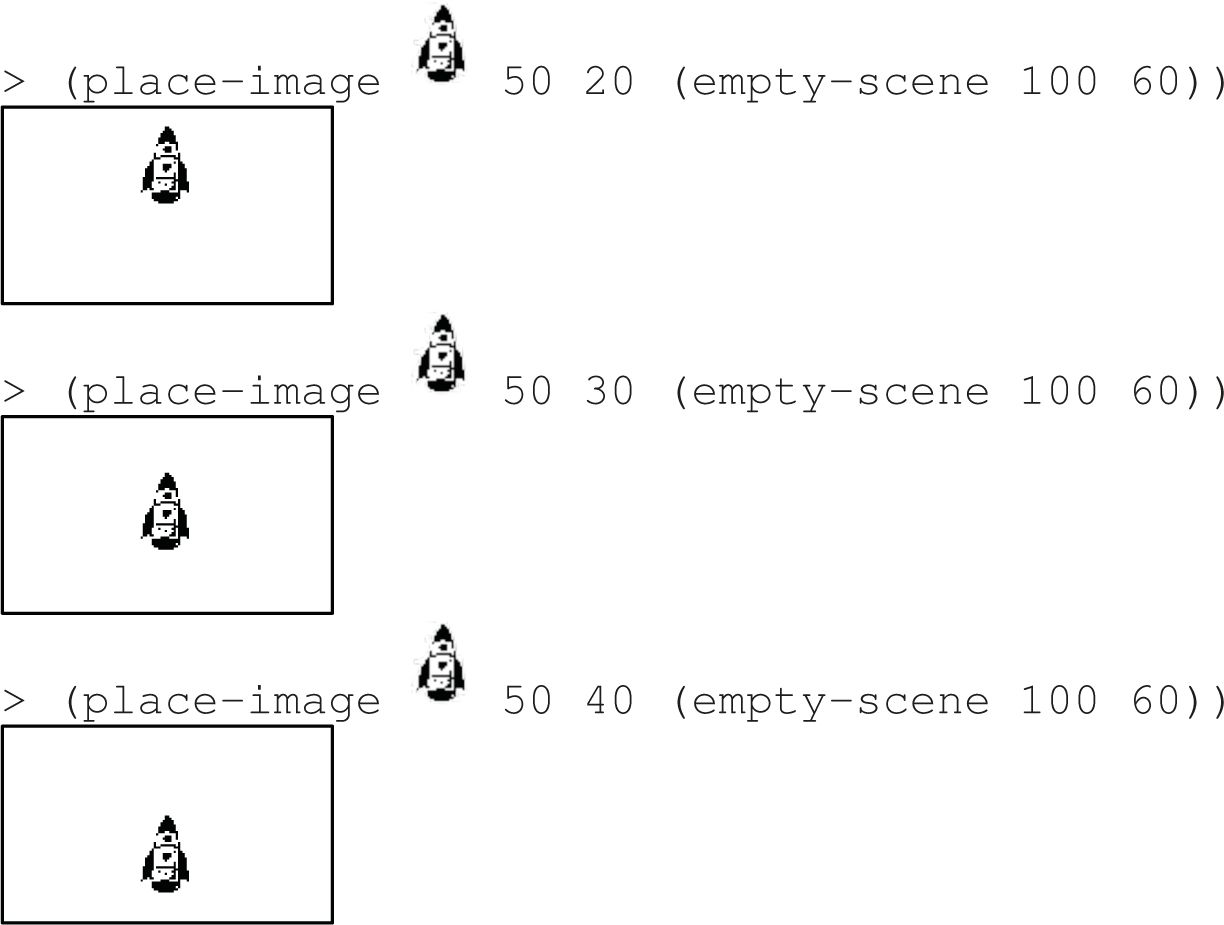
\includegraphics[width=0.75\textwidth]{images/00019.jpeg}
\end{center}

现在剩下的唯一任务，就是如何轻松大量地生成这类连续场景，并以极快的速度依次将它们连续播放出来。

第一个目标当然可以通过定义一个函数轻松达成，参见图~\ref{fig:rocket_v1}。没错，这是一个货真价实的函数定义！我们没有使用晦涩单调的字母 \code{y}，而是为其赋予了一个顾名思义的名称 \code{picture-of-rocket}（火箭画面），一眼就能看出该函数的输出是一个包含火箭的场景画面。在参数命名上，我们没有使用抽象的字母 \code{x}，而是采用了 \code{height}（高度），这直观表明它是一个数字，且明确告诉函数应当将火箭放置在场景中的哪个高度位置。函数体表达式与我们刚才反复操练的表达式完全相同，唯一的不同在于用形参 \code{height} 替换了具体的硬编码数字。现在，我们可以利用这一个函数轻松创建任意高度的画面：
\begin{lstlisting}[language=BSL]
(picture-of-rocket 0)
(picture-of-rocket 10)
(picture-of-rocket 20)
(picture-of-rocket 30)
\end{lstlisting}

\begin{figure}[htbp]
  \centering
\begin{stepperbox}[unbreakable]
\begin{Verbatim}[commandchars=\\\{\}, fontsize=\scriptsize]
(define (picture-of-rocket height)
  (place-image \inlinesprite[1.4em]{images/sprites/rocket.png} 50 height (empty-scene 100 60)))
\end{Verbatim}
\end{stepperbox}
  \caption{火箭降落程序（版本 1）}
  \label{fig:rocket_v1}
\end{figure}

在定义区或交互区中输入上述调用；两者都能立刻生成完全符合预期的连续画面。

\begin{notebox}[BSL 标识符命名规范]
在 BSL 中，你可以使用各种丰富的字符来为函数或变量命名，包括连字符“\code{-}”和点号“\code{.}”，这让名称具备极佳的自解释性。
\end{notebox}

要达成第二个目标（快速连续播放生成动态电影），我们需要从 \code{2htdp/universe} 教学包中请出一位关键原语：\term{animate}（动画控制器）。点击“Run”，在交互区中输入以下神奇的表达式：
\begin{replbox}
> (animate picture-of-rocket)
\end{replbox}

\begin{notebox}[引入动画教学包]
别忘了在定义区最上方添加 \code{(require 2htdp/universe)}，以导入宇宙/世界程序库。
\end{notebox}

停下来，请特别注意：\textbf{这里的参数本身是一个函数名}！目前不必对将函数作为参数感到深奥或顾虑；它在 \code{animate} 中工作得极其出色，不过初学阶段暂且不要尝试自己编写像 \code{animate} 这样以函数作为参数的高阶函数。

当你按下回车键的一刹那，DrRacket 会立刻对该表达式求值；但它并不会在交互区输出任何普通的静态文本，甚至提示符也不会立刻出现。相反，它会单独弹出一个崭新的独立动画窗口（画布），并启动一个每秒钟跳动 28 次的高精度时钟！每当时钟滴答跳动一次，DrRacket 就会自动调用 \code{picture-of-rocket} 函数，并将“自启动以来所流逝的时钟滴答总数”（0、1、2、3……）作为实参传入。这些函数调用所生成的场景画面被源源不断地刷新绘制在画布上，从而在视网膜上形成了流畅逼真的动态火箭降落动画！动画会一直持续运行，直到你手动关闭该窗口为止；此时 \code{animate} 会在交互区返回动画总共经历的时钟滴答数。

这个动画背后的本质运行机制是什么？简短的解释是：\code{animate} 将其操作数（即传入的函数）依次应用于数字 0、1、2、3……并实时呈现生成的连续画面。详细的机制如下：
\begin{itemize}
  \item \code{animate} 启动一个独立时钟，并对滴答步数进行自增计数；
  \item 时钟以每秒 28 次的恒定频率跳动；
  \item 每次时钟滴答，\code{animate} 都会以当前时钟计数为参数调用 \code{picture-of-rocket} 函数；
  \item 该次调用所返回的全新场景被立即投射显示在动画画布上。
\end{itemize}

这意味着小火箭首先出现在高度 0 处，接着是高度 1、高度 2……这完美解释了为什么小火箭会从画布顶部平稳地降落到底部。也就是说，我们仅仅用了区区三行代码的微型程序，就在短短 3.5 秒内自动生成了约 100 张连续画面，并通过超高速放映创造出逼真的火箭降落视觉奇观！

\begin{notebox}[关于 animate 的原理]
在全书后半部分的练习 298 中，我们将带领大家亲手从底层设计实现出属于自己的 \code{animate} 核心引擎。
\end{notebox}

回顾本节，你学到了至关重要的核心知识：函数之所以威力无穷，是因为它们能够在极短时间内批量自动化处理海量数据。你可以手动在少数几个精心挑选的典型输入上测试函数，以确保它产出完全正确的预期结果，这被称为\term{测试函数}（testing a function）。或者，DrRacket 可以在各类外部库的配合下，自动在海量数据流上连续调用该函数，这被称为\term{运行函数}（running a function）。自然，DrRacket 也能在用户敲击键盘或滑动鼠标时自动触发函数的调用。究竟是什么事件触发了函数的执行并不重要，但请永远牢记：\textbf{（简单）程序在本质上就是函数}。


% ------------------------------------------------------------------------------
\section{多样化的计算方式}
\label{sec:prologue:many_ways}
% ------------------------------------------------------------------------------

当你运行 \code{(animate picture-of-rocket)} 时，小火箭最终会直直地穿透场景底部并沉入地底深渊消失不见。这显然违背常识。在老科幻电影中，火箭绝不会无休止地遁入地心，而是会优雅地用尾部平稳着陆在地面上，动画也应当在着陆的瞬间圆满落幕。

这一需求表明：\textbf{计算应当根据现实情境的不同，走向截然不同的逻辑分支}。在我们的案例中，当火箭尚在空中飞行时，\code{picture-of-rocket} 应当按原样绘制动态下落；然而一旦火箭的尾部触及画布底部，程序就应当立即阻止火箭继续下潜。

从某种意义上说，这种思想对你而言毫不陌生。甚至连中学数学老师在定义函数时，也会根据不同情形进行条件分流：

\[
  \mathrm{sign}(x) = \begin{cases}
    +1 & \text{if } x > 0 \\
    \phantom{+}0 & \text{if } x = 0 \\
    -1 & \text{if } x < 0
  \end{cases}
\]

这个符号函数 $\mathrm{sign}(x)$ 明确区分了三种输入情境：大于 0 的正数、等于 0 的数值以及小于 0 的负数。根据输入落入的区间，函数分别返回 $+1$、$0$ 或 $-1$。

在 DrRacket 中，你可以借助\term{条件表达式}（conditional expression，简称 \code{cond}）毫无困难地将这种分段函数原汁原味地翻译为代码：

\begin{lstlisting}[language=BSL]
(define (sign x)
  (cond
    [(> x 0) 1]
    [(= x 0) 0]
    [(< x 0) -1]))
\end{lstlisting}

点击“Run”后，你就可以像测试任何普通函数一样在交互区与 \code{sign} 进行交互：
\begin{replbox}
> (sign 10)
1
> (sign -5)
-1
> (sign 0)
0
\end{replbox}

\begin{notebox}[在 DrRacket 中开启新标签页]
可以在 DrRacket 中点击“File”菜单选择“New Tab”（新建标签页），开启一个干干净净的全新工作区进行实验。
\end{notebox}

在语法结构上，条件表达式的一般形式如下：
\begin{lstlisting}[language=BSL]
(cond
  [ConditionExpression1 ResultExpression1]
  [ConditionExpression2 ResultExpression2]
  ...
  [ConditionExpressionN ResultExpressionN])
\end{lstlisting}

\begin{notebox}[探索代数单步求值器]
现在是体验 DrRacket 中“Step”（单步求值器）神奇魅力的绝佳时机！在定义区添加 \code{(sign -5)}，然后点击工具栏右上角的“Step”按钮。在弹出的单步求值器窗口中，点击左右箭头，亲眼观察表达式一步一步被替代求值的全过程！
\end{notebox}

也就是说，一个条件表达式由若干行条件分支（clauses）构成。每一行包含两个子表达式：位于左侧的通常称为\term{条件}（condition，有时也称问题/断言），位于右侧的称为\term{结果}（result，有时也称答案）。当 DrRacket 对一个 \code{cond} 表达式进行求值时，它首先计算第一个条件表达式 \code{ConditionExpression1}：
\begin{itemize}
  \item 如果求值结果为 \code{\#true}，DrRacket 会立刻将整个 \code{cond} 表达式替换为对应的 \code{ResultExpression1}，对其求值并将该值作为整个条件表达式的最终结果；
  \item 如果求值结果为 \code{\#false}，DrRacket 会彻底忽略该分支，转而对下一行重复相同的判定；
  \item 如果所有行的条件表达式求值结果均为 \code{\#false}，DrRacket 会直接报错，指出没有满足任何条件分支。
\end{itemize}

掌握了这一利器，我们现在便能从容改变火箭模拟动画的运转轨迹了。目标是：绝不让小火箭下降到 100 $\times$ 60 场景的地面以下。由于 \code{picture-of-rocket} 函数接收一个代表火箭在场景中所处高度的数字实参，只需引入一个简单的测试，将传入的当前高度与最大极限高度进行比对即可。

参见图~\ref{fig:rocket_v2} 中的修正后函数定义。为了区分两个版本，我们在新定义中使用名称 \code{picture-of-rocket.v2}。使用不同的函数名还允许我们在交互区同时调用两个版本，并直观对比它们的行为差异。以下是最初版本 1 的运行效果：

\begin{center}
  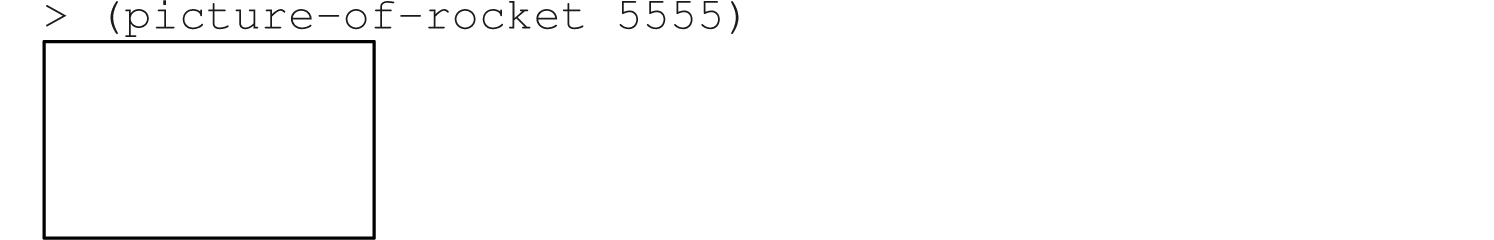
\includegraphics[width=0.85\textwidth]{images/00023.png}
\end{center}

\begin{figure}[htbp]
  \centering
\begin{stepperbox}[unbreakable]
\begin{Verbatim}[commandchars=\\\{\}, fontsize=\footnotesize]
(define (picture-of-rocket.v2 height)
  (cond
    [(<= height 60)
     (place-image \inlinesprite[1.4em]{images/sprites/rocket.png} 50 height
                  (empty-scene 100 60))]
    [(> height 60)
     (place-image \inlinesprite[1.4em]{images/sprites/rocket.png} 50 60
                  (empty-scene 100 60))]))
\end{Verbatim}
\end{stepperbox}
  \caption{火箭降落程序（版本 2）}
  \label{fig:rocket_v2}
\end{figure}

以下是全新版本 2 的运行效果：

\begin{center}
  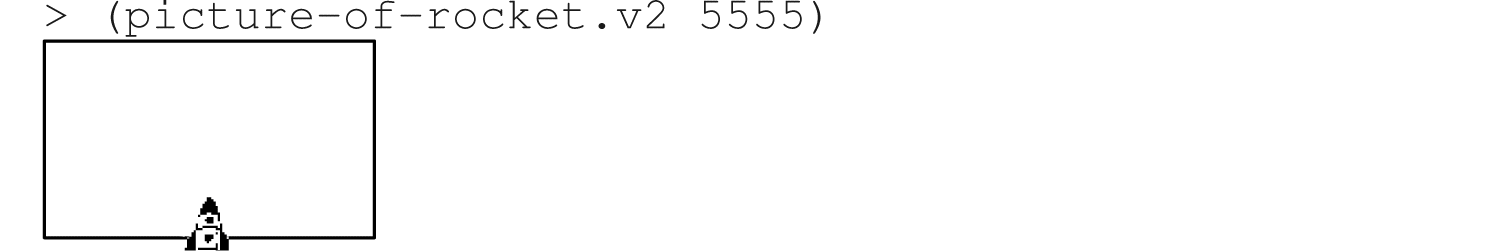
\includegraphics[width=0.85\textwidth]{images/00025.png}
\end{center}

无论你传递给 \code{picture-of-rocket.v2} 多大的数字，只要它超过了 60，得到的永远是同一幅固定在底部的画面。特别地，当你在交互区执行：
\begin{replbox}
> (animate picture-of-rocket.v2)
\end{replbox}
小火箭在下降后，会在正好陷进地面一半的位置赫然停住！

\begin{notebox}[思考提问]
停下来想一想！这真的是我们期望看到的完美着陆吗？
\end{notebox}

让火箭半截身子陷进泥土里显然很不雅观。不过，你完全清楚如何修复这一瑕疵。正如你所见，BSL 精通图像算术。当 \code{place-image} 将一幅图像绘制到场景中时，它默认将该图像的\textbf{几何中心点}作为对齐锚点，尽管图像本身拥有真实的物理宽度与高度。你一定还记得，我们可以使用 \code{image-height} 随时测量出图像的准确高度。这个操作在这里派上了大用场，因为我们真正希望的是：让火箭平稳飞行，直到其\textbf{底面触及地面}的那一刻停止。

把各方线索串联起来，你就能通过算术推导出：

\begin{stepperbox}
\begin{Verbatim}[commandchars=\\\{\}, fontsize=\footnotesize]
(- 60 (/ (image-height \inlinesprite[1.4em]{images/sprites/rocket.png}) 2))
\end{Verbatim}
\end{stepperbox}

正是火箭停止下降时其中心点应当停留的准确位置！你可以通过直接修改程序来验证这一推断，也可以在交互区利用图像算术即时验证。

以下是初步的尝试：

\begin{stepperbox}
\begin{Verbatim}[commandchars=\\\{\}, fontsize=\footnotesize]
(place-image \inlinesprite[1.4em]{images/sprites/rocket.png} 50 (- 60 (image-height \inlinesprite[1.4em]{images/sprites/rocket.png}))
             (empty-scene 100 60))
\end{Verbatim}
\end{stepperbox}

现在，把上面调用中的第三个实参替换为：

\begin{stepperbox}
\begin{Verbatim}[commandchars=\\\{\}, fontsize=\footnotesize]
(- 60 (/ (image-height \inlinesprite[1.4em]{images/sprites/rocket.png}) 2))
\end{Verbatim}
\end{stepperbox}

\begin{notebox}[动手实验]
停下来，在 DrRacket 中亲身运行对比这两个调用。你更钟意哪一个视觉呈现？
\end{notebox}

沿着这一思路深入思考与反复验证，最终你就会自然而然地写出如图~\ref{fig:rocket_v3} 所示的优雅程序。给定一个代表火箭飞行高度的数字，它首先检测火箭的底端是否尚在地表之上。如果是，它像以前一样将火箭绘制在当前飞行高度；如果不是，它将火箭放置在底端正好贴合地面的精确几何位置！

\begin{figure}[htbp]
  \centering
\begin{stepperbox}[unbreakable]
\begin{Verbatim}[commandchars=\\\{\}, fontsize=\scriptsize]
(define (picture-of-rocket.v3 height)
  (cond
    [(<= height (- 60 (/ (image-height \inlinesprite[1.4em]{images/sprites/rocket.png}) 2)))
     (place-image \inlinesprite[1.4em]{images/sprites/rocket.png} 50 height
                  (empty-scene 100 60))]
    [(> height (- 60 (/ (image-height \inlinesprite[1.4em]{images/sprites/rocket.png}) 2)))
     (place-image \inlinesprite[1.4em]{images/sprites/rocket.png} 50 (- 60 (/ (image-height \inlinesprite[1.4em]{images/sprites/rocket.png}) 2))
                  (empty-scene 100 60))]))
\end{Verbatim}
\end{stepperbox}
  \caption{火箭降落程序（版本 3）}
  \label{fig:rocket_v3}
\end{figure}


% ------------------------------------------------------------------------------
\section{一个程序，多个定义}
\label{sec:prologue:one_program_many_definitions}
% ------------------------------------------------------------------------------

现在设想你的朋友们观赏了你的火箭降落动画，但他们觉得默认的画布尺寸太局促了，希望能将其扩展为 200 $\times$ 400 的宽阔大场景。面对这个看似简单的需求变更，你不得不痛苦地在程序中的五个不同地方把 100 逐一替换为 400，在另外两个地方把 60 逐一替换为 200——更不必说代码中那些代表“画布水平中线”的数字 50 了。

\begin{notebox}[动手体验硬编码之痛]
在继续阅读前，请务必停下来动手尝试手动修改这些数字！亲身体验一下在区区五行代码的程序中完成这一改动是多么容易漏改改错。在阅读后续内容时，请时刻牢记：现实工业界中的软件规模往往长达 50,000 行、500,000 行乃至 5,000,000 行以上的庞大代码库！
\end{notebox}

在一个设计优良的理想程序中，一个微小的需求调整（比如修改画布尺寸），应当仅仅需要对应一处微小的代码修改。在 BSL 中实现这一优雅解耦的利器依然是 \code{define}。除了定义函数，\code{define} 还能用于定义\term{常量}（constants），即将一个有意义的名字与一个固定常量值绑定在一起。常量定义的一般形式极为简洁：
\begin{lstlisting}[language=BSL]
(define Name Expression)
\end{lstlisting}

举例来说，如果在程序中写下：
\begin{lstlisting}[language=BSL]
(define HEIGHT 60)
\end{lstlisting}
你就是在向 DrRacket 声明：全局名称 \code{HEIGHT} 始终代表数字 60。这种定义的语义完全符合常识：每当 DrRacket 在后续计算中遇到标识符 \code{HEIGHT} 时，它都会自动用 60 替换之。

现在请仔细审视遵照这一设计原则重构出的图~\ref{fig:rocket_v4}。它落实了这一改动，并且为小火箭图像也赋予了一个直观的名字。将该程序复制到 DrRacket 中，点击“Run”后在交互区执行：
\begin{replbox}
> (animate picture-of-rocket.v4)
\end{replbox}
确认该程序的功能与之前的版本 3 完全一致。

\begin{figure}[htbp]
  \centering
\begin{stepperbox}[unbreakable]
\begin{Verbatim}[commandchars=\\\{\}, fontsize=\scriptsize]
(define (picture-of-rocket.v4 h)
  (cond
    [(<= h (- HEIGHT (/ (image-height ROCKET) 2)))
     (place-image ROCKET 50 h (empty-scene WIDTH HEIGHT))]
    [(> h (- HEIGHT (/ (image-height ROCKET) 2)))
     (place-image ROCKET
                  50 (- HEIGHT (/ (image-height ROCKET) 2))
                  (empty-scene WIDTH HEIGHT))]))

(define WIDTH 100)
(define HEIGHT 60)
(define ROCKET \inlinesprite[1.4em]{images/sprites/rocket.png})
\end{Verbatim}
\end{stepperbox}
  \caption{火箭降落程序（版本 4）}
  \label{fig:rocket_v4}
\end{figure}

图~\ref{fig:rocket_v4} 中的程序共包含四个顶层定义：一个函数定义与三个常量定义。数字 100 与 60 在整个程序中各自仅出现了一次——分别作为 \code{WIDTH} 与 \code{HEIGHT} 的值。你可能还注意到，我们将函数形参从 \code{height} 缩写为了 \code{h}。严格来说这一修改并非必需，因为 DrRacket 能够严格区分小写的 \code{height} 与大写的常量 \code{HEIGHT}，但为了避免读者在视觉上产生混淆，我们特意做了区分。

当 DrRacket 执行 \code{(animate picture-of-rocket.v4)} 时，每当它在计算中遇到这些名字，都会自动将 \code{HEIGHT} 替换为 60、\code{WIDTH} 替换为 100、\code{ROCKET} 替换为具体的火箭图像。为了亲身体验真正程序员的高光时刻，请将 \code{HEIGHT} 后面的 60 改为 400，然后轻点“Run”。你将瞬间看到小火箭在宽 100、高 400 的宏大高空场景中优雅降落！\textbf{仅仅改动一个数字，全局牵一发而动全身}。

在现代软件工程术语中，你刚刚亲身经历了人生的第一次\term{代码重构}（program refactoring）。每当你为了让程序更好地适应未来潜在的需求变更而重新梳理和优化其架构时，你都在对程序进行重构。把这个词骄傲地写进你的简历吧，它听起来专业干练，你未来的雇主一定会乐于看到这样的工程素养。然而，任何一个真正优秀的程序员都绝不可能容忍在同一个程序中将完全相同的子表达式重复书写三次：
\begin{lstlisting}[language=BSL]
(- HEIGHT (/ (image-height ROCKET) 2))
\end{lstlisting}

每当你的同事或未来的你自己阅读这段代码时，都必须费神去重新推导该表达式究竟在算什么（即场景顶部到落地火箭中心点的距离）。每当 DrRacket 计算该表达式时，它都必须死板地重复三步计算：(1) 测量图像高度；(2) 除以 2；(3) 从 \code{HEIGHT} 中减去该值。而且每一次算出的都是完全相同的定值！

这一观察强烈呼唤我们引入一个新的常量定义：
\begin{lstlisting}[language=BSL]
(define ROCKET-CENTER-TO-TOP
  (- HEIGHT (/ (image-height ROCKET) 2)))
\end{lstlisting}

现在，在程序的其余部分中，用名字 \code{ROCKET-CENTER-TO-TOP} 彻底替换掉那长长的一串表达式。你可能会琢磨：这个新常量定义到底应该放在 \code{HEIGHT} 之上还是之下？更普适地讲，程序中定义的排列顺序是否至关重要？答案是：\textbf{对于常量定义，先后顺序至关重要；而对于函数定义，顺序则完全无关紧要}。一旦 DrRacket 读到一个常量定义，它会立即对等号右边的表达式求值，并立即将名称与该结果值永久绑定。例如：
\begin{lstlisting}[language=BSL]
(define HEIGHT (* 2 CENTER))
(define CENTER 100)
\end{lstlisting}
会导致 DrRacket 在执行第一行时严厉报错：“\code{CENTER} 在定义之前就被使用了”。相反：
\begin{lstlisting}[language=BSL]
(define CENTER 100)
(define HEIGHT (* 2 CENTER))
\end{lstlisting}
则完全顺畅运行。首先，DrRacket 将 \code{CENTER} 绑定为 100；其次，对 \code{(* 2 CENTER)} 求值得出 200；最后，将 200 绑定至 \code{HEIGHT}。

尽管常量之间的定义先后顺序不可颠倒，但常量定义相对于函数定义的相对位置却完全自由。事实上，如果你的程序由许多函数定义组成，函数彼此之间的摆放顺序也完全任意；但最佳的工程实践是：\textbf{首先集中声明所有全局常量定义，随后按照重要程度降序排列各个函数定义}。当你日后开始独立编写包含数十个定义的复杂大型项目时，你就会深刻体会到这种清晰组织纪律的无穷益处。

\begin{notebox}[关于代码注释]
程序中还可以包含以分号（\code{;}）开头的单行注释。尽管 DrRacket 运行时会彻底忽略所有注释，但阅读代码的人类绝不应忽视它们。注释是程序的创作者与未来的维护者之间跨越时空的“秘密沟通热线”，用于传递代码本身难以自述的架构意图。
\end{notebox}

一旦清除了所有重复冗余的表达式，我们便收获了如图~\ref{fig:rocket_v5} 所示的纯净版本。它由一个主函数定义与五个精心提炼的常量定义组成。除了火箭落地中心点位置外，这些常量还将火箭图像资源本身以及空白背景场景的构建完全抽取成了独立组件。

\begin{figure}[htbp]
  \centering
\begin{stepperbox}[unbreakable]
\begin{Verbatim}[commandchars=\\\{\}, fontsize=\scriptsize]
; constants
(define WIDTH  100)
(define HEIGHT  60)
(define MTSCN  (empty-scene WIDTH HEIGHT))
(define ROCKET \inlinesprite[1.4em]{images/sprites/rocket.png})
(define ROCKET-CENTER-TO-TOP
  (- HEIGHT (/ (image-height ROCKET) 2)))

; functions
(define (picture-of-rocket.v5 h)
  (cond
    [(<= h ROCKET-CENTER-TO-TOP)
     (place-image ROCKET 50 h MTSCN)]
    [(> h ROCKET-CENTER-TO-TOP)
     (place-image ROCKET 50 ROCKET-CENTER-TO-TOP MTSCN)]))
\end{Verbatim}
\end{stepperbox}
  \caption{火箭降落程序（版本 5）}
  \label{fig:rocket_v5}
\end{figure}

在继续翻页之前，请结合版本 5 深入思考并尝试动手实现以下改进：
\begin{itemize}
  \item 如何修改程序，使其呈现 200 $\times$ 400 的宽阔场景？
  \item 如何修改程序，使其降落的不再是火箭，而是一个绿色的不明飞行物（UFO 飞碟）？绘制飞碟其实极其容易：
\begin{lstlisting}[language=BSL]
(overlay (circle 10 "solid" "green")
         (rectangle 40 4 "solid" "green"))
\end{lstlisting}
  \item 如何修改程序，使太空背景始终呈现出深邃的纯蓝色？
  \item 如何修改程序，让火箭最终停靠在一块比场景底部高出 10 像素的平坦岩石停机坪上？别忘了相应更新背景场景中的地貌绘制！
\end{itemize}

心动不如行动。亲自编写与调试代码是掌握程序设计的唯一康庄大道。别犹豫，现在就打开 DrRacket 大展身手吧！

\paragraph{告别魔法数字（Magic Numbers）}
再次仔细打量 \code{picture-of-rocket.v5}。因为我们消除了所有重复表达式，除却一个数字外，所有的字面数值都从该函数定义中彻底消失了。在专业编程领域，那些散落在代码深处不知其意的裸露数字被称为\term{魔法数字}（magic numbers），没有任何专业工程师会喜欢它们。因为要不了多久，你自己都会忘却这个数字在几何运算中究竟代表什么含义、哪些改动是安全合法的。最稳健的策略始终是用一个有意义的常量定义为其命名。

在这里我们清楚知道：数字 50 代表我们为小火箭选定的水平 $x$ 坐标。尽管单个数字 50 看起来算不上复杂的长算式，但它在本质上也是一个反复出现的重复表达式。因此，我们有充分的理由将 50 从函数体中提炼出来，这个小练习就作为礼物留给你亲手完成吧！


% ------------------------------------------------------------------------------
\section{再添一个定义}
\label{sec:prologue:one_more_definition}
% ------------------------------------------------------------------------------

请回想一下：\code{animate} 传递给其处理函数的实参，本质上是自启动以来\textbf{所经历的时钟滴答总数}！也就是说，传入 \code{picture-of-rocket} 的参数根本不是什么“高度”，而是“\textbf{时间}”。我们之前在所有版本的 \code{picture-of-rocket} 中使用的形参名称其实全都是错误的；我们不应使用代表高度的 \code{h}，而应当使用代表时间的 \code{t}：

\begin{lstlisting}[language=BSL]
(define (picture-of-rocket t)
  (cond
    [(<= t ROCKET-CENTER-TO-TOP)
     (place-image ROCKET 50 t MTSCN)]
    [(> t ROCKET-CENTER-TO-TOP)
     (place-image ROCKET
                  50 ROCKET-CENTER-TO-TOP
                  MTSCN)]))
\end{lstlisting}

而对参数命名的这一微小修正，立刻把程序深层隐藏的一个荒谬漏洞暴露无遗：这个程序竟然把“时间”硬生生当成了“空间距离”来使用！这是多么离谱的设计纰漏啊。

\begin{notebox}[危险预警]
本节需要引入一条基础的初中物理常识。如果你对物理感到头疼，初读时大可放心略过；真正的日常程序设计通常并不需要你通晓物理学知识。
\end{notebox}

即使你从未学过物理，你也必定知晓时间与位移绝非同一物理量。我们的程序之所以之前能跑得有模有样，完全是碰巧撞大运的偶然巧合。不过完全不必惊慌，修正这一切易如反掌。我们所需要的全部“火箭科学”，不过是一点点大家熟知的初等物理运动学定律。

物理学？！是的。也许你早已把当年课堂上学过的公式抛到九霄云外，或者你因为年纪尚小根本还没有接触过物理课。放轻松！这在最顶尖的专业程序员职业生涯中也是司空见惯的日常：程序员每天都要跨界协助音乐家、经济学家、摄影师、医护人员等各行各业的专业人士解决专业领域的计算难题。显而易见，没有任何程序员能够全知全能。因此他们会在需要时查阅资料，或者直接向领域专家请教。如果你去请教一位物理学家，他会立刻告诉你：做匀速运动的物体，其移动的位移与所经历的时间成正比：

\[
  d = v \cdot t
\]

也就是说，如果一个物体的运动速度为 $v$，那么该物体在时间 $t$ 秒内所走过的距离为 $d$ 英里（或米、像素等等）。

当然，一位严谨的老师应当向你展示规范的函数记法：

\[
  d(t) = v \cdot t
\]

因为这种记法能向所有人明确传达：$d$ 的计算依赖于自变量 $t$，而 $v$ 则是一个恒定的常数。作为一名专业程序员，我们会走得更远，用具有鲜明语义的英文单词替换这些单字母简写：
\begin{lstlisting}[language=BSL]
(define V 3)
(define (distance t)
  (* V t))
\end{lstlisting}

这段程序片段由两个清晰的定义组成：函数 \code{distance} 负责计算以恒定速度运动的物体所走过的位移，常量 \code{V} 则明确描述了其速度大小。

你可能会好奇为什么这里的速度 \code{V} 设为了 3？并没有什么玄机，我们只是觉得每时钟滴答下移 3 个像素是一个匀速优雅的下落速度。你完全可以自由微调这个数字，并在动画中亲眼观察小火箭速度的快慢变化。

现在我们终于能够彻底完美地重构 \code{picture-of-rocket} 了！函数不再将时间 $t$ 错误地与高度进行比较，而是调用 \code{(distance t)} 来精确计算火箭当前应当下移的物理距离。最终的完整程序展示在图~\ref{fig:rocket_v6} 中。它由两个函数定义协同工作：\code{picture-of-rocket.v6} 与 \code{distance}。其余的常量定义则赋予了程序极佳的可读性与易维护性。一如既往，你可以用 \code{animate} 启动这个完美的动画：
\begin{replbox}
> (animate picture-of-rocket.v6)
\end{replbox}

\begin{figure}[htbp]
  \centering
\begin{stepperbox}[unbreakable]
\begin{Verbatim}[commandchars=\\\{\}, fontsize=\scriptsize]
; properties of the "world" and the descending rocket
(define WIDTH  100)
(define HEIGHT  60)
(define V 3)
(define X 50)

; graphical constants
(define MTSCN  (empty-scene WIDTH HEIGHT))
(define ROCKET \inlinesprite[1.4em]{images/sprites/rocket.png})
(define ROCKET-CENTER-TO-TOP
  (- HEIGHT (/ (image-height ROCKET) 2)))

; functions
(define (picture-of-rocket.v6 t)
  (cond
    [(<= (distance t) ROCKET-CENTER-TO-TOP)
     (place-image ROCKET X (distance t) MTSCN)]
    [(> (distance t) ROCKET-CENTER-TO-TOP)
     (place-image ROCKET X ROCKET-CENTER-TO-TOP MTSCN)]))

(define (distance t)
  (* V t))
\end{Verbatim}
\end{stepperbox}
  \caption{火箭降落程序（版本 6）}
  \label{fig:rocket_v6}
\end{figure}

与最初简陋的火箭程序相比，版本 6 清晰地向我们揭示了现代软件工程的真实面貌：\textbf{一个软件系统通常由若干个相互协作、相互调用的子函数有机组合而成}。其实即便利在版本 1 中，我们也调用了 \code{+} 与 \code{/}——只是以前你把它们看作语言原生的内置运算符而已。

随着你一步步成长为真正的专业程序员，你会发现现实中的大型程序正是由成百上千个函数定义与常量定义精妙交织而成的。你还会发现，函数之间彼此调用是程序世界的绝对常态。你真正需要刻意操练的核心本领，是\textbf{系统化地组织架构它们}，使得即使在数月甚至数年之后，任何人翻开代码依然能一目了然、轻松理解。毕竟，未来的你自己（或是接手项目的其他同事）总有一天需要对这些代码进行修改扩展；如果你无法清晰理解程序的组织脉络，哪怕面对最微小的功能调整，你都会陷入举步维艰的痛苦境地。至此，关于基础编程机制的一切要义，你已尽在掌握。


% ------------------------------------------------------------------------------
\section{你现在是程序员了}
\label{sec:prologue:programmer_now}
% ------------------------------------------------------------------------------

在读完上一节末尾时，得知自己已经是一名程序员的断言或许会让你感到有些猝不及防，但事实确凿无疑！你已经彻底掌握了关于 BSL 语法的全部机械机制。你明白编程所依靠的不仅是数字算术，更是包括字符串、布尔值、图像以及任何未来语言所支持的丰富数据形态在内的“广义算术”。你深知程序是由函数定义与常量定义有机组装起来的。你更明白——因为我们刚刚耳提面命地叮嘱过你——编程的终极艺术归根结底在于如何清晰有条理地组织管理这些定义。最后但同样重要的一点是，你已经知晓 DrRacket 与各类教学包提供了海量开箱即用的强大函数，并且学会了如何随时在 DrRacket 的 HelpDesk 文档中检索它们的使用指南。

你或许仍会心存疑虑：自己还没学会怎么编写响应键盘按键、鼠标点击等复杂人机交互的程序呢，怎么能算真正的程序员？然而真相是：你早已具备了所需的一切底蕴！除了 \code{animate} 函数外，\code{2htdp/universe} 教学包还提供了一整套标准函数，能够将你的函数无缝挂接到计算机的键盘、鼠标、系统时钟以及各种输入设备上。事实上，它甚至内置了网络通信支持，允许你编写出将自己的电脑与全球任何一台电脑相连的分布式网络程序。因此，这根本算不上什么障碍。

简而言之，关于将代码拼接成运行程序的机械机制，你几乎已经全盘领略。只要查阅相关函数的 API 文档，你完全有能力写出富有趣味的电脑小游戏、科学仿真模拟软件或是商业记账系统。然而，核心的拷问在于：这一切真的意味着你已经成为一名合格的程序员了吗？你是吗？

\begin{notebox}[深度沉思]
停下来！先不要急着翻到下一页。认真思考这个问题！
\end{notebox}


% ------------------------------------------------------------------------------
\section{才怪！}
\label{sec:prologue:not}
% ------------------------------------------------------------------------------

当你漫步在任何一家书店的书架前，瞥见计算机编程专区时，总会看到铺天盖地的图书在大肆宣扬能够让你“立竿见影、速成成为程序员”。然而，在亲手完成了前面的初探性探索之后，你心中必定已经清醒地意识到：这种神话绝无可能成真。

仅仅掌握编程的机械技巧——学会写出计算机能理解的表达式、熟悉各种库函数与 API 等等——对于从事\textbf{真正}的程序设计而言，并没有太大实质性的助益。如果光靠这些就能成为程序员，那么一个人只要死记硬背下词典里的几千个单词再背上几条语法规则，岂不就等于精通了一门外国语言？

\term{优良的程序设计}，其内涵远比单纯掌握一门语言的语法机制深邃得多。最核心的法则在于：程序员必须时刻铭记，\textbf{代码是写给未来的其他人阅读的}！一个优秀的程序应当忠实映照出问题陈述本身及其核心领域概念。它应当配备言简意赅的自解释说明。详实的功能示例能够将这种说明具象化，并将其紧密锚定在原始问题上。这些示例能确保未来的读者能够清清楚楚地领会你的代码究竟为何如此工作。简而言之，优秀的程序设计关乎\textbf{系统化地解决现实问题}，并将这种严谨的系统思考清晰贯穿于代码之中。最美妙的是，这种以系统为核心的方法论真正使程序设计向所有人敞开了大门——它兼顾了工程严谨与普适教学的两大至高追求。

本书的全部精髓，正是全心全意传授这些经得起时间检验的真谛；书中真正关于 DrRacket 软件操作、BSL 语法细节或外部库调用的篇幅其实少之又少。本书将为你全面展现优秀程序员面对复杂问题时是如何深入思考与谋篇布局的。此外你还会惊喜地发现：这种严谨解决问题的心智模型，能够完美普适于现实生活中的各种复杂挑战，无论是医生诊疗、记者调研、律师辩护还是工程师设计。

顺便提一句：本书在后续正式章节中所采用的叙述语调，将会比这篇活泼的序幕更加严谨深沉、契合经典学术巨著的厚重底蕴。愿你在这趟奇妙的计算之旅中满载而归！

\begin{notebox}[关于本书不涵盖什么的说明]
市面上许多编程入门书籍往往热衷于夹带作者个人钟爱的特定应用学科私货：数论难题、高深数学、物理模拟、音乐合成等。此类材料固然无可厚非，因为编程在所有这些领域都大有用武之地；然而它们却往往严重喧宾夺主，极大地分散了学生对程序设计核心本质的注意力。因此，我们在本书中竭尽全力将对外部学科背景知识的依赖降至最低，以便能够全神贯注地聚焦于计算机科学能够为你带来的核心财富：\textbf{计算化解决问题的普适思维能力}。
\end{notebox}


\mainmatter

% ==================== 第一部分：固定大小的数据 ====================
\part{固定大小的数据 (Fixed-Size Data)}
% ==============================================================================
% 第 1 章：算术 (Chapter 1: Arithmetic)
% ==============================================================================

\chapter{算术}
\label{sec:ch01_arithmetic}

在序幕中，你已经学会了如何用初学学生语言（BSL）的记法来书写小学一年级就学过的算术表达式：
\begin{itemize}
  \item 写下左括号 \code{(}；
  \item 写下原生操作的名称 \code{op}；
  \item 写下操作的操作数（参数），各参数之间用空格分隔；
  \item 写下右括号 \code{)}。
\end{itemize}

作为回顾，这里给出一个最基本的原生表达式：
\begin{lstlisting}[language=BSL]
(+ 1 2)
\end{lstlisting}

它使用了加法操作符 \code{+} 来对两个数进行相加，其后跟着两个操作数，它们都是普通的数。但再看下面这个例子：
\begin{lstlisting}[language=BSL]
(+ 1 (+ 1 (+ 1 1) 2) 3 4 5)
\end{lstlisting}

第二个例子体现了上述语法规则中两个极其强大的特点：第一，原生操作可以接收两个以上的参数；第二，参数本身不一定必须是孤立的数值，它们也可以是嵌套的表达式。

\begin{notebox}[阅读建议]
快速浏览本章，直接跳到第~2~章；后续当你遇到不认识的“算术运算”时，再随时翻回本章查阅。
\end{notebox}

表达式的求值过程同样直截了当。首先，BSL 计算原生操作的所有参数表达式的值；其次，将计算得到的数据“喂给”该操作，由它计算出最终结果。因此：
\begin{lstlisting}[language=BSL]
(+ 1 2) == 3
\end{lstlisting}
以及：
\begin{lstlisting}[language=BSL]
(+ 1 (+ 1 (+ 1 1) 2) 3 (+ 2 2) 5)
== (+ 1 (+ 1 2 2) 3 4 5)
== (+ 1 5 3 4 5)
== 18
\end{lstlisting}

这些计算步骤对你来说应该十分熟悉，因为它们与你在数学课上所做的一模一样。你可能以前书写演算步骤的格式有所不同，或者从未系统学过如何一步步写下演算序列。但请放心，BSL 的计算法则与你从小掌握的算术完全一致，这足以令人心安。它保证了你能够清晰理解计算机对原生数据和原生操作做了什么，从而能够准确推导和预测程序的计算结果。一般而言，程序员必须深入透彻地理解编程语言的计算模型，否则程序的错误运算可能会危害到系统的使用者或其代表的利益。

\begin{notebox}[关于等号符号]
本书中使用记号 \code{==} 表示“根据计算法则两边完全等价”。
\end{notebox}

本章接下来的内容将介绍 BSL 的四种\term{原子数据}（atomic data）：数（Number）、字符串（String）、图像（Image）以及布尔值（Boolean）。我们借用了物理学中的“原子”概念：你无法窥探单个原子数据的内部构造，但可以通过函数将多个原子数据组合成新的数据，或者提取它们的属性（属性本身也是原子数据）等。本章各节将介绍处理这些数据的函数，它们通常被称为\term{原生操作}（primitive operations）或预定义操作。你也可以在 DrRacket 自带的 BSL 官方帮助文档中找到更多操作。

\begin{notebox}[进阶提示]
下一卷《How to Design Components》将深入解释如何自行设计原子数据。
\end{notebox}


% ==============================================================================
% 1.1 数的算术
% ==============================================================================
\section{数的算术}
\label{sec:1.1}

大多数人听到“算术”二字时，脑海中浮现的都是“数字”以及“对数字的操作”。“对数字的操作”意味着将两个数相加得到第三个数、从一个数中减去另一个数、计算两个数的最大公约数等等。如果我们不把算术限制得过于狭隘，它甚至可以包含计算角度的正弦值、将实数四舍五入为最接近的整数等数学运算。

BSL 语言原生支持数（Number）以及针对数的算术运算。正如序幕中所讨论的，加法等算术操作采用\term{前缀记法}（prefix notation）：
\begin{lstlisting}[language=BSL]
(+ 3 4)
\end{lstlisting}

语言为我们提供了非常丰富的数值操作：\code{+}、\code{-}、\code{*}、\code{/}、\code{abs}、\code{add1}、\code{ceiling}、\code{denominator}、\code{exact->inexact}、\code{expt}、\code{floor}、\code{gcd}、\code{log}、\code{max}、\code{numerator}、\code{quotient}、\code{random}、\code{remainder}、\code{sqr} 以及 \code{tan} 等等。我们只是按照字母顺序挑出了一些代表性的操作来展示其多样性。你可以在交互区中探索它们的用途，并去文档中看看还有哪些可用操作。

只要是你在数学课上学过的数值操作，BSL 大多都已经内置支持了。不妨猜猜它的函数名，并在交互区动手试一试。比如你需要计算某个角度的正弦值：
\begin{replbox}
> (sin 0)
0
\end{replbox}
你就可以放心使用它了。或者去查阅 DrRacket 的帮助手册（HelpDesk）。你会在手册中发现，除了丰富的数学函数外，BSL 还预定义了一些著名常数的名字，例如 \code{pi}（圆周率 $\pi$）和 \code{e}（自然常数 $e$）。

\begin{notebox}[常数 $e$（自然常数）]
你可能在微积分中接触过常数 $e$。它是一个实数，约等于 $2.718$，被称为“欧拉常数”或自然底数。
\end{notebox}

在数的种类上，BSL 程序可以使用自然数、整数、有理数、实数以及复数。我们假定你对除了复数之外的其他数都已相当熟悉。复数可能在高中数学课上提到过；如果没有也不必担心，虽然复数在科学计算中极其有用，但作为初学者完全无需掌握复数也能畅通无阻。

关于数值，一个极其关键的概念是\term{精度}（precision）。在现阶段，最重要的是理解 BSL 将数明确划分为\term{精确数}（exact numbers）与\term{不精确数}（inexact numbers）。在处理精确数时，BSL 尽可能全程保持完全精度。例如计算 \code{(/ 4 6)} 会产生精确的分数 \code{2/3}，DrRacket 可以将其呈现为真分数、假分数或混合小数。你可以用鼠标右键点击结果，在弹出菜单中切换分数的显示格式。

BSL 的某些数值操作无法产生精确结果。例如对 $2$ 使用 \code{sqrt}（开平方）操作，会产生一个无法用有限位数精确表示的无理数。由于计算机内存空间是有限的，BSL 必须将该数值适配到计算机中，因此会采用近似浮点数：\code{1.4142135623730951}。正如序幕中所提及的，前缀 \code{\#i} 会明确警示初学者该结果是不精确的。尽管绝大多数现代编程语言都通过降低精度来处理此类计算，但极少有语言能像 BSL 这样明确标注并主动提醒程序员。

\begin{notebox}[关于数的术语说明]
术语“数”（Number）指代了广泛的数值集合，包括计数、整数、有理数、实数乃至复数。在大多数日常场景中，你尽可以把 Number 等同于小学数轴上的数。当需要更加严谨时，我们会使用更精准的术语：Integer（整数）、Rational（有理数）等。甚至可以使用标准术语进行更细致的限定，如 PositiveInteger（正整数）、NonnegativeNumber（非负数）、NegativeNumber（负数）等。
\end{notebox}

\begin{exercise}{两点间距离计算}{1}
将以下针对 \code{x} 和 \code{y} 的定义添加到 DrRacket 的定义区：
\begin{lstlisting}[language=BSL]
(define x 3)
(define y 4)
\end{lstlisting}

现在将 \code{x} 和 \code{y} 想象为平面直角坐标系中一个点的横纵坐标。请写出一个表达式，计算该点到坐标原点 $(0,0)$ 的距离。

对于上述给定的初始值，预期的计算结果是 $5$。但你的表达式应当具备通用性：无论修改定义区中 \code{x} 和 \code{y} 的值为何，点击运行后都能正确计算出对应的距离。

如果你还没学过平面几何，或者忘记了相关公式，点 $(x,y)$ 到原点的欧几里得距离公式如下：
\[
  \sqrt{x^2 + y^2}
\]
毕竟我们的目标是教会你如何设计程序，而不是培养几何学家。

要构造这个表达式，最好的方法是点击【运行】（RUN）按钮并在交互区中进行交互式尝试。RUN 操作会让 DrRacket 获知 \code{x} 和 \code{y} 的当前值，这样你就能测试包含 \code{x} 和 \code{y} 的表达式：
\begin{replbox}
> x
3
> y
4
> (+ x 10)
13
> (* x y)
12
\end{replbox}

一旦在交互区找到了能得出正确结果的表达式，将其复制粘贴到定义区中。

为了检验表达式是否具有通用性，将定义区中的 \code{x} 修改为 \code{12}，\code{y} 修改为 \code{5}，再次点击【运行】，结果应当输出 \code{13}。
\end{exercise}

你的数学老师会说你刚刚计算了“距离公式”。为了在不同输入上复用该公式，你必须每次打开 DrRacket，编辑 \code{x} 和 \code{y} 的定义使其代表目标坐标，然后点击运行。但这种复用公式的方式既繁琐又笨拙。在第~2~章中，我们将很快为你介绍\term{函数}（function）的定义方法，它能让公式的复用变得极其优雅自然。目前安排此类练习，是为了引出函数思想，并为你即将开始的函数式编程做好铺垫。


% ==============================================================================
% 1.2 字符串的算术
% ==============================================================================
\section{字符串的算术}
\label{sec:1.2}

关于计算机内部运作，人们普遍存在一种偏见：许多人认为计算机内部全都是比特（bit）和字节（byte）——不论那到底是什么——并且充其量只能处理数字，因为人人都知道计算机会算术。诚然，电气工程师必须以这种方式理解和研究硬件，但初学者及其他任何应用开发者绝不需要（永远不需要）陷入这种底层思维。

编程语言的核心是处理\term{信息}（information），而现实世界的信息形态万千、各具特色。例如，程序可能需要处理颜色、人名、商务信函或人与人之间的对话。尽管我们理论上可以用一堆数字把所有信息都编码（例如规定 0 代表“红色”，1 代表“你好”），但这绝对是个糟糕至极的主意。试想一下，光是记忆庞大的对照表就会让人痛苦不堪。

因此，现代编程语言至少都会提供一种专门处理文本符号信息的数据类型。在 BSL 中，我们使用\term{字符串}（String）。通俗地说，字符串就是由双引号包围的字符序列，其中的字符可以通过键盘输入。在序幕中我们已经见过很多 BSL 字符串：\code{"hello"}、\code{"world"}、\code{"blue"}、\code{"red"} 等等。前两个是日常对话或信件中的词汇；后两个则是我们想要使用的颜色名称。

\begin{notebox}[关于 1String 的说明]
我们使用 \term{1String} 指代构成字符串的单个字符。例如，\code{"red"} 由三个 1String 构成：\code{"r"}、\code{"e"} 和 \code{"d"}。虽然在技术实现上 1String 有更完备的定义，但目前将其视为长度为 1 的字符串即可。
\end{notebox}

BSL 中只有一个专门接收字符串并产出字符串的原生操作：\code{string-append}。正如我们在序幕中所见，它将给定的多个字符串拼接为一个整体。可以将 \code{string-append} 理解为字符串世界的 \code{+}。加法接收两个（或更多）数字并产生一个新数字；拼接操作则接收两个（或更多）字符串并产生一个新字符串：
\begin{replbox}
> (string-append "what a " "lovely " "day" " 4 BSL")
"what a lovely day 4 BSL"
\end{replbox}

就像 \code{+} 相加时不会破坏或更改原有的数字一样，\code{string-append} 拼接时也绝不会篡改任何传入的字符串。要演算此类表达式，只需应用显而易见的运算法则即可：
\begin{center}
  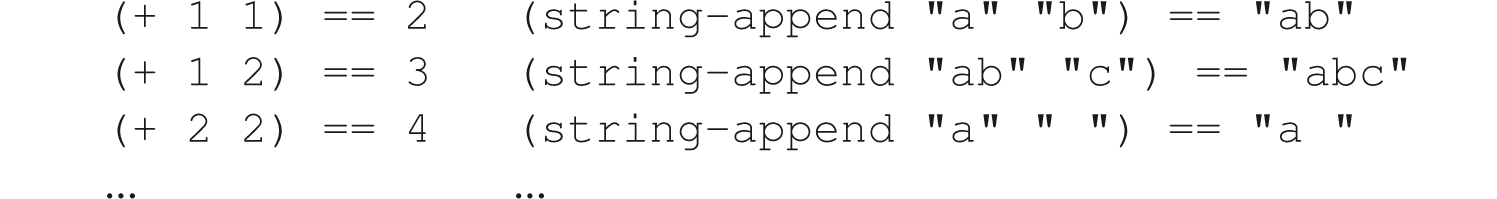
\includegraphics[width=0.7\textwidth]{images/00039.png}
\end{center}

\begin{exercise}{字符串拼接与连接符}{2}
在定义区添加以下两行代码：
\begin{lstlisting}[language=BSL]
(define prefix "hello")
(define suffix "world")
\end{lstlisting}

然后使用字符串原生操作编写一个表达式，将 \code{prefix} 与 \code{suffix} 拼接起来，并在两者中间插入下划线 \code{"\_"}。运行程序后，交互区应当输出 \code{"hello\_world"}。

参考练习~\ref{ex:1} 了解如何在 DrRacket 中测试与组织表达式。
\end{exercise}


% ==============================================================================
% 1.3 混合运算
% ==============================================================================
\section{混合运算}
\label{sec:1.3}

BSL 中所有其他与字符串相关的操作，要么接收非字符串数据，要么产生非字符串数据。以下是一些典型示例：
\begin{itemize}
  \item \code{string-length}：接收一个字符串，返回其字符个数（数）；
  \item \code{string-ith}：接收一个字符串 \code{s} 和一个整数 \code{i}，提取位于第 \code{i} 个位置的 1String（从 0 开始计数）；
  \item \code{number->string}：接收一个数，将其转换为对应的字符串。
\end{itemize}

请在帮助手册中查找并阅读 \code{substring} 的说明，了解它的具体功能。

如果文档中的描述一时难以理解，不妨直接在交互区中亲自实验这些函数。传入合适的参数观察其输出；也可以故意传入不合法的参数，看看 BSL 会如何报错：
\begin{replbox}
> (string-length 42)
string-length: expects a string, given 42
\end{replbox}

如你所见，BSL 会报告明确的错误信息。前半部分 \code{string-length} 指出哪个函数被误用了；后半部分则指明传入的参数错在何处。在这个例子中，\code{string-length} 期望接收一个字符串，但实际给入的却是一个数（即 42）。

当然，只要你清楚每个操作的输入输出类型，就可以自由地将处理不同类型数据的操作嵌套在一起。思考序幕中的这个表达式：
\begin{lstlisting}[language=BSL]
(+ (string-length "hello world") 20)
\end{lstlisting}

内层表达式对字符串 \code{"hello world"} 调用 \code{string-length}；外层表达式则让 \code{+} 将内层的结果与 \code{20} 相加。我们一步步推导该表达式的值：
\begin{lstlisting}[language=BSL]
(+ (string-length "hello world") 20)
== (+ 11 20)
== 31
\end{lstlisting}

不出所料，这种涉及不同数据类型的复合表达式的计算，与纯数值算术没有任何本质区别。再看另一个例子：
\begin{lstlisting}[language=BSL]
(+ (string-length (number->string 42)) 2)
== (+ (string-length "42") 2)
== (+ 2 2)
== 4
\end{lstlisting}

在继续学习之前，请尝试构造几个错误混合数据类型的嵌套表达式，例如：
\begin{lstlisting}[language=BSL]
(+ (string-length 42) 1)
\end{lstlisting}
在 DrRacket 中运行它们。仔细观察红色的错误提示信息，并注意观察定义区中被高亮标出的出错位置。

\begin{exercise}{在指定位置插入字符}{3}
在定义区添加以下两行：
\begin{lstlisting}[language=BSL]
(define str "helloworld")
(define i 5)
\end{lstlisting}

然后使用字符串原生函数编写一个表达式，在第 \code{i} 个位置插入下划线 \code{"\_"}。通常这意味着生成的新字符串会比原字符串更长；在当前测试中，预期结果为 \code{"hello\_world"}。

位置（position）表示从字符串最左端开始偏移的字符数，但程序员从 0 开始计数。因此在当前例子中，第 5 个字符是 \code{"w"}，因为第 0 个字符是 \code{"h"}。

\textbf{计数提示：}遇到此类索引计数问题时，可以在 \code{str} 下方添加一个数字索引字符串来辅助观察：
\begin{lstlisting}[language=BSL]
(define str "helloworld")
(define ind "0123456789")
(define i 5)
\end{lstlisting}
\end{exercise}

\begin{exercise}{删除指定位置的字符}{4}
沿用练习~\ref{ex:3} 中的相同设定，编写一个表达式，从字符串 \code{str} 中删除第 \code{i} 个位置的字符。显然，这个新字符串会比原字符串短一个字符。对于给定的字符串，\code{i} 取哪些值是合法且有效的？
\end{exercise}


% ==============================================================================
% 1.4 图像的算术
% ==============================================================================
\section{图像的算术}
\label{sec:1.4}

\term{图像}（Image）是一种可视化的二维矩形数据，例如照片、几何图形或绘图画布。在 DrRacket 中，凡是可以书写表达式的地方都可以直接插入图像，因为图像也是一等值（Value），与数和字符串处于同等地位。

\begin{notebox}[图像库引入]
在新的代码窗口中使用图像功能前，请务必在定义区顶部声明：\code{(require 2htdp/image)}。
\end{notebox}

你的程序可以通过原生操作来创建与变换图像。这些原生图像操作主要分为三大类。第一类用于创建基础图形：
\begin{itemize}
  \item \code{circle}：根据半径、填充模式和颜色创建圆形；
  \item \code{ellipse}：根据横向半径、纵向半径、填充模式和颜色创建椭圆；
  \item \code{line}：根据两点相对位移和颜色绘制线段；
  \item \code{rectangle}：根据宽度、高度、填充模式和颜色创建矩形；
  \item \code{text}：根据文本内容、字号和颜色渲染文本图像；
  \item \code{triangle}：根据边长、填充模式和颜色创建顶点向上的等边三角形。
\end{itemize}

这些操作的名称清晰指明了所创建图形的种类。你只需要知道，模式参数通常是 \code{"solid"}（实心）或 \code{"outline"}（轮廓线），而颜色参数是如 \code{"orange"}、\code{"black"} 等颜色名称字符串。

在交互区中实际尝试这些操作，如图~\ref{fig:ch01_image_intro} 所示：
\begin{figure}[htbp]
  \centering
  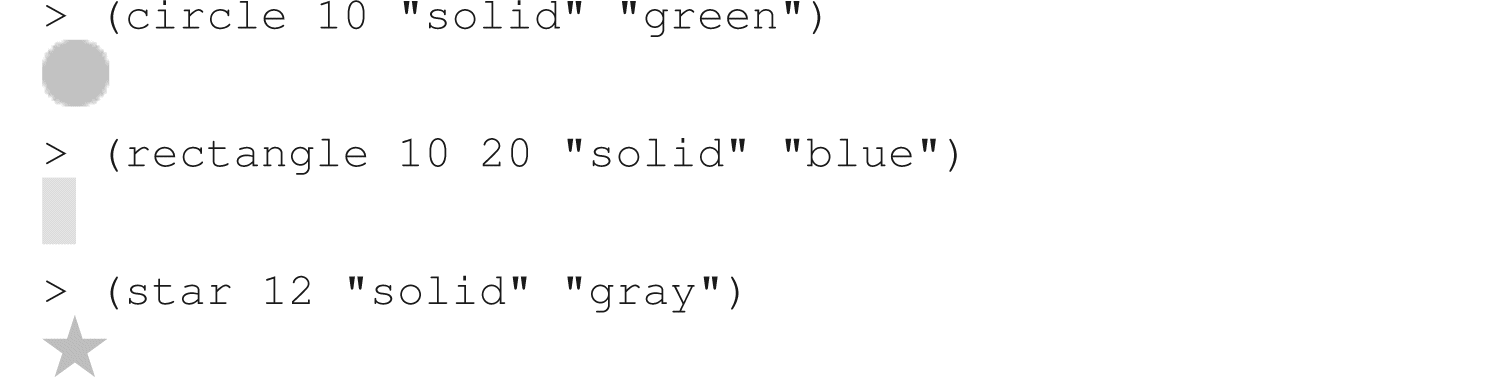
\includegraphics[width=0.75\textwidth]{images/00040.png}
  \caption{在交互区中测试基础图形创建操作}
  \label{fig:ch01_image_intro}
\end{figure}

请停下来思考！上面这段截图中出现了一个前文未提及的操作。请查阅帮助文档，看看 \code{2htdp/image} 库中还提供了哪些基础图形绘制函数，并亲自实验探索。

第二类图像函数用于测量图像属性：
\begin{itemize}
  \item \code{image-width}：以像素为单位获取图像的宽度；
  \item \code{image-height}：以像素为单位获取图像的高度。
\end{itemize}

它们能从图像中提取出符合直觉的数值：
\begin{replbox}
> (image-width (circle 10 "solid" "red"))
20
> (image-height (rectangle 10 20 "solid" "blue"))
20
\end{replbox}

请停下来思考！解释 DrRacket 是如何一步步求出以下表达式的值的：
\begin{lstlisting}[language=BSL]
(+ (image-width (circle 10 "solid" "red"))
   (image-height (rectangle 10 20 "solid" "blue")))
\end{lstlisting}

为了透彻理解第三类图像组合操作，需要引入一个新概念：\term{锚点}（anchor point）。图像不是孤立的单个像素，而是由许多像素构成的矩形区域。每个图像都像一张照片，其矩形范围内部有一个隐式的基准锚点。当你使用图像合成函数将两张图像叠合时，除非明确指定，否则默认都是围绕各自的锚点对齐的：
\begin{itemize}
  \item \code{overlay}：将传入的多个图像依次叠放在一起，默认以各自的中心点作为对齐锚点；
  \item \code{overlay/xy}：类似于 \code{overlay}，但在两个图像之间额外接收两个数值 \code{x} 和 \code{y}。它将第二张图像相对于第一张图像的左上角向右平移 \code{x} 像素，向下平移 \code{y} 像素；负的 \code{x} 向左移动，负的 \code{y} 向上移动；
  \item \code{overlay/align}：类似于 \code{overlay}，但接收两个字符串指定对齐边缘（例如 \code{"center"}、\code{"left"}、\code{"right"}、\code{"top"}、\code{"bottom"} 等），共有 9 种可能的对齐组合。
\end{itemize}

\code{2htdp/image} 库还包含了许多用于合成图像的高级函数。随着你逐步熟悉图像处理，可以进一步阅读文档。目前我们再介绍三个关键函数，它们对于构建游戏和交互动画至关重要：
\begin{itemize}
  \item \code{empty-scene}：创建指定宽度和高度的空白矩形画布（场景）；
  \item \code{place-image}：将一张图像放置在场景中的指定坐标位置。如果图像超出了画布边界，超出部分会被自动裁切；
  \item \code{scene+line}：接收一个场景、两点坐标数值和颜色，在场景上绘制一条直线。
\end{itemize}

图像算术的演算法则与数的算术完全类似；参见图~\ref{fig:ch01_image_laws} 中给出的示例及其与数值算术的对照。同样，任何原始图像都不会被修改或破坏，这些操作只是依据输入合成了全新的图像对象。

\begin{figure}[htbp]
  \centering
  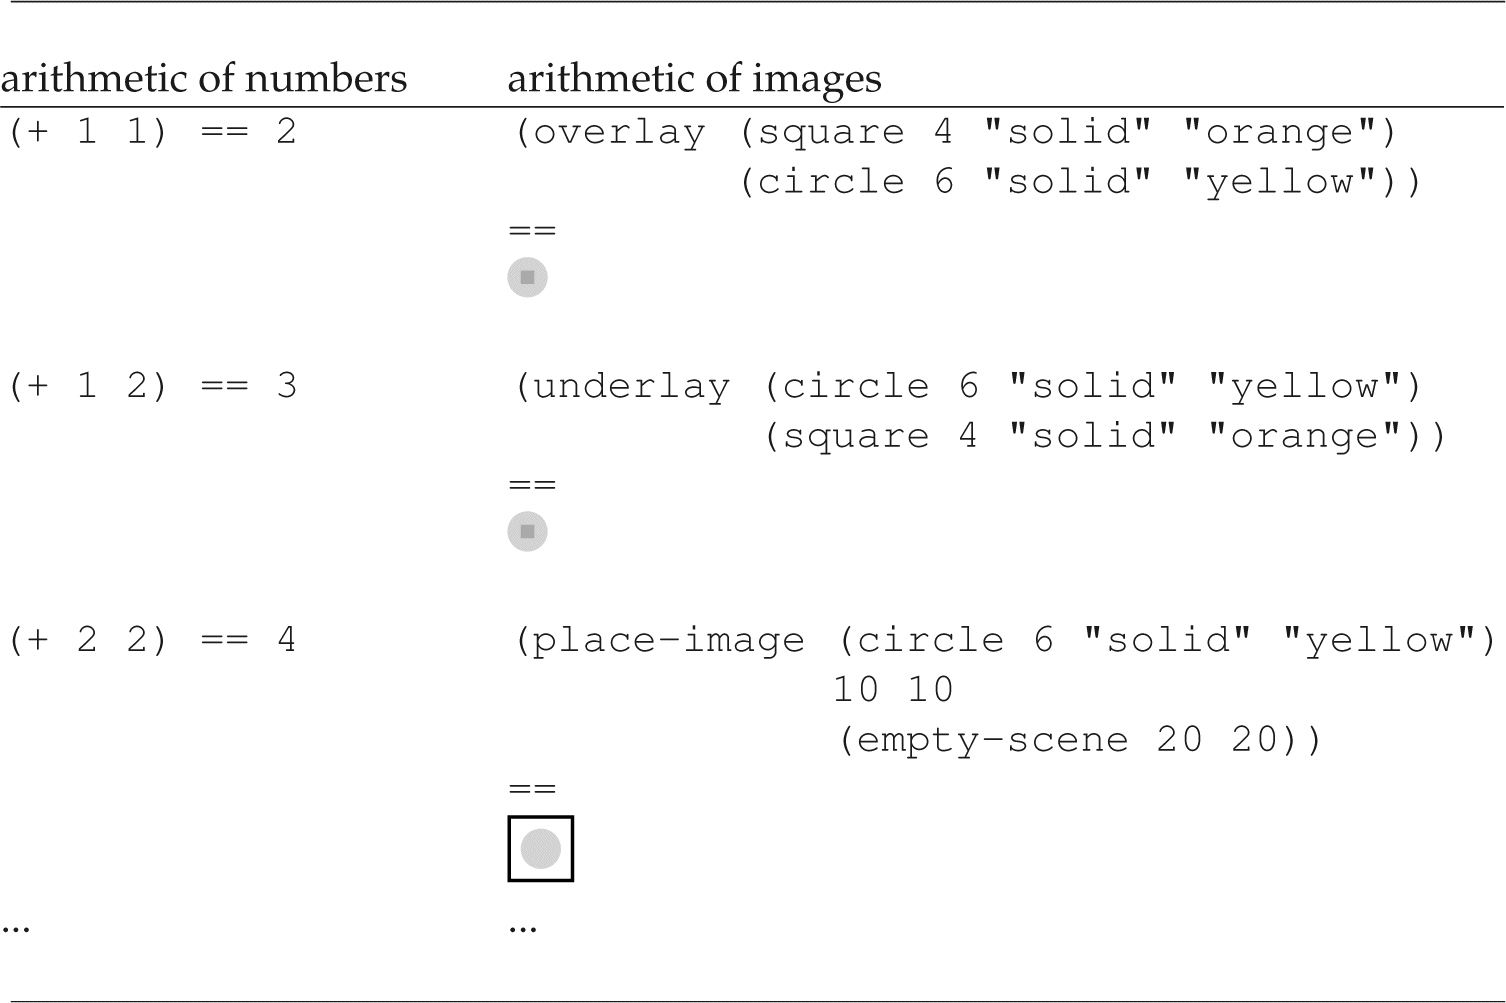
\includegraphics[width=0.85\textwidth]{images/00041.png}
  \caption{图像构造的代数演算法则与数值计算的类比}
  \label{fig:ch01_image_laws}
\end{figure}

\begin{exercise}{创建小船或小树图像}{5}
使用 \code{2htdp/image} 库中的绘图函数，拼装出一艘简易小船或一棵小树的图像。注意在设计代码时保持清晰结构，使得后续能够方便地通过修改参数来整体缩放图像大小。
\end{exercise}

\begin{exercise}{计算图像的像素数}{6}
在定义区添加以下代码：
\begin{center}
  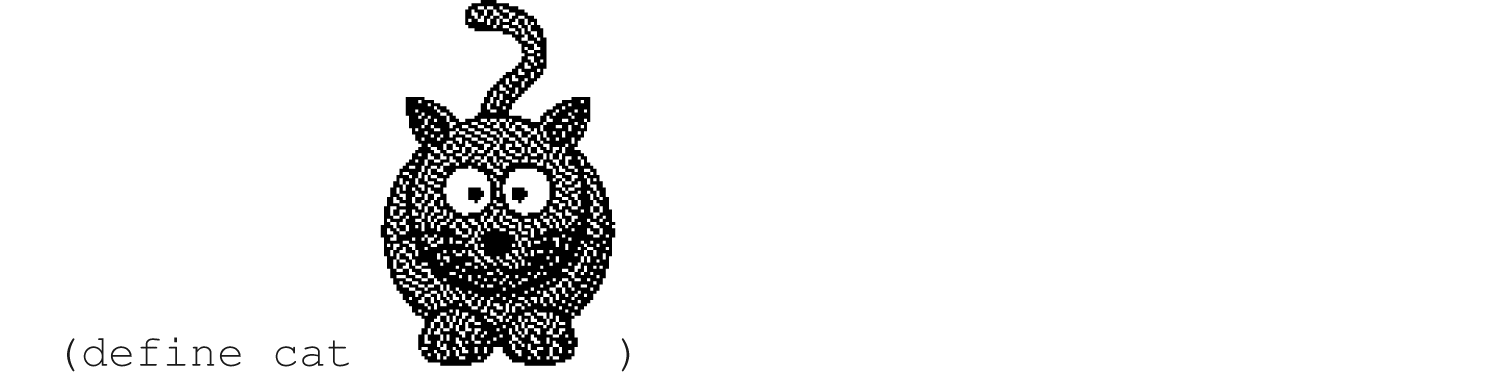
\includegraphics[width=0.55\textwidth]{images/00042.png}
\end{center}

\textbf{图片复制技巧：}你可以直接从电子书中复制该小猫图片，并直接粘贴到 DrRacket 的定义区代码中。

编写一个表达式，计算该图像所包含的总像素数（即像素面积）。
\end{exercise}


% ==============================================================================
% 1.5 布尔值的算术
% ==============================================================================
\section{布尔值的算术}
\label{sec:1.5}

在正式动手设计程序之前，我们还需要掌握最后一种基础原子数据：\term{布尔值}（Boolean values）。布尔值只有两个：\code{\#true} 和 \code{\#false}。在程序中，布尔值主要用来表示条件决策的结果或各种开关的状态。

布尔值的运算同样非常简单。BSL 程序主要使用三个逻辑操作：\code{or}（逻辑或）、\code{and}（逻辑与）和 \code{not}（逻辑非）。它们在逻辑世界中的角色，就像数的加法、乘法与取相反数。由于布尔值只有两种可能，我们可以穷举列出所有可能情况下的运算行为：
\begin{itemize}
  \item \code{or}：检查传入的布尔值中是否存在任意一个 \code{\#true}：
\begin{replbox}
> (or #true #true)
#true
> (or #true #false)
#true
> (or #false #true)
#true
> (or #false #false)
#false
\end{replbox}

  \item \code{and}：检查传入的布尔值是否全部都为 \code{\#true}：
\begin{replbox}
> (and #true #true)
#true
> (and #true #false)
#false
> (and #false #true)
#false
> (and #false #false)
#false
\end{replbox}

  \item \code{not}：逻辑取反，总是返回与给定布尔值相反的值：
\begin{replbox}
> (not #true)
#false
> (not #false)
#true
\end{replbox}
\end{itemize}

和加法类似，\code{or} 与 \code{and} 也可以接收两个以上的布尔表达式。另外，\code{or} 和 \code{and} 还有短路求值等更深刻的特性，这需要我们在更复杂的嵌套表达式中进一步探究。

\begin{exercise}{商场购物条件判断}{7}
布尔表达式能够精确描述许多日常生活中的决策逻辑。假设你想决定今天是否适合去商场逛街。你的决策准则是：只要“今天不是晴天”或者“今天是周五”（因为商场周五会推出全新打折特卖），你就去商场。

按照你刚刚学到的布尔运算知识，首先在 DrRacket 定义区添加以下两行：
\begin{lstlisting}[language=BSL]
(define sunny #true)
(define friday #false)
\end{lstlisting}

现在编写一个表达式，判断在“\code{sunny} 为假”或者“\code{friday} 为真”时是否前往商场。在当前的具体设定下，计算结果应当是 \code{\#false}（为什么？）。

请参考练习~\ref{ex:1} 组织测试。\code{sunny} 和 \code{friday} 两个变量一共有多少种不同的布尔值组合？
\end{exercise}


% ==============================================================================
% 1.6 布尔混合运算
% ==============================================================================
\section{布尔混合运算}
\label{sec:1.6}

布尔值的一大核心用途是与其他类型的数据协同进行条件计算。在序幕中我们知道，BSL 允许通过定义为数据命名。例如，我们可以用以下代码开始一个程序：
\begin{lstlisting}[language=BSL]
(define x 2)
\end{lstlisting}
然后计算其倒数：
\begin{lstlisting}[language=BSL]
(define inverse-of-x (/ 1 x))
\end{lstlisting}
这在平时运转良好，但如果我们把 \code{x} 的值修改为 \code{0}，程序就会因除以零而崩溃。

这就凸显了布尔值与条件分支的威力。首先，原生判断函数 \code{=} 用来判断两个（或多个）数是否相等。如果相等则返回 \code{\#true}，否则返回 \code{\#false}。其次，BSL 提供了条件分支形式：\term{\code{if} 表达式}。\code{if} 的用法看起来类似原生函数，但它实际上是核心语法形式。\code{if} 后面跟随三个子表达式，各部分以空格分隔，整体由括号包围：
\begin{lstlisting}[language=BSL]
(if (= x 0) 0 (/ 1 x))
\end{lstlisting}

该 \code{if} 表达式包含了三个子表达式：\code{(= x 0)}、\code{0} 以及 \code{(/ 1 x)}。\code{if} 表达式的求值严格遵循两步法则：
\begin{enumerate}
  \item 首先必定对第一个条件子表达式求值，其计算结果必须是一个布尔值（\code{\#true} 或 \code{\#false}）；
  \item 若条件为 \code{\#true}，则对第二个子表达式求值并将其作为整个 \code{if} 的结果；若条件为 \code{\#false}，则对第三个子表达式求值并作为结果。
\end{enumerate}

在给定 \code{x} 为 2 的定义下，你可以在交互区中试验该表达式：
\begin{replbox}
> (if (= x 0) 0 (/ 1 x))
0.5
\end{replbox}

根据代数计算法则，你可以自行手动推导其求值步骤：
\begin{lstlisting}[language=BSL]
(if (= x 0) 0 (/ 1 x))
== ; 因为全局变量 x 的当前值为 2
(if (= 2 0) 0 (/ 1 2))
== ; 2 不等于 0，(= 2 0) 计算结果为 #false
(if #false 0 (/ 1 2))
== ; if 分支依据 #false 选取第三个子表达式
(/ 1 2)
== ; 转换为十进制显示
0.5
\end{lstlisting}

换句话说，DrRacket 知道 \code{x} 代表 2 且不等于 0，因此 \code{(= x 0)} 得到 \code{\#false}，驱动 \code{if} 仅计算第三个子表达式 \code{(/ 1 x)}，完全避免了潜在的除以零错误！

请停下来思考！假设将定义区修改为：
\begin{lstlisting}[language=BSL]
(define x 0)
\end{lstlisting}
在此时的环境下，\code{(if (= x 0) 0 (/ 1 x))} 会计算出什么结果？为什么？请写出一步步的演算序列。

除 \code{=} 外，BSL 还提供了全套数值比较操作符：\code{<}（小于）、\code{<=}（小于等于）、\code{>}（大于）和 \code{>=}（大于等于）。请解释它们各自的判断规则。

注意：字符串不能使用 \code{=} 进行比较。如果需要比较字符串，必须使用专门的字符串比较操作符：\code{string=?}、\code{string<=?} 或 \code{string>=?}。\code{string=?} 显然是判断两个字符串内容是否完全一致，而后两者则是按字典序进行比较。你可以查阅文档并动手验证。

你可能会好奇，为什么程序需要比较字符串？想象一个控制红绿灯交通信号灯的程序，它可能使用字符串 \code{"green"}、\code{"yellow"} 和 \code{"red"} 来表示灯的颜色。程序中可能包含类似下面的片段：
\begin{lstlisting}[language=BSL]
(define current-color ...)
(define next-color
  (if (string=? "green" current-color) "yellow" ...))
\end{lstlisting}
显然，这段代码负责根据当前灯的颜色计算下一个应当点亮的状态。

在接下来的章节中，我们将介绍比简单的 \code{if} 更强大、更优雅的条件表达式（例如 \code{cond}），以及设计复杂条件分支的系统化方法。

\begin{exercise}{图像长宽比分类}{8}
在定义区添加以下代码：
\begin{center}
  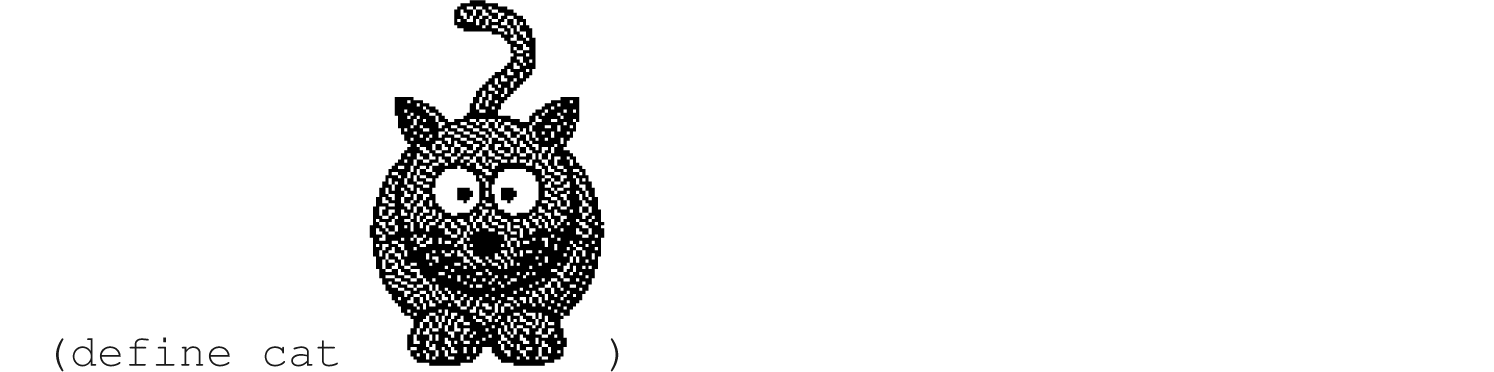
\includegraphics[width=0.55\textwidth]{images/00043.png}
\end{center}

编写一个条件表达式，判断该图像是瘦高形（\code{"tall"}）还是矮宽形（\code{"wide"}）。如果高度大于等于宽度，判定为 \code{"tall"}；否则判定为 \code{"wide"}。在测试时，可以把小猫图片临时替换为你自己创建的不同长宽的矩形，以确保能够预测并验证答案。

进一步拓展：修改你的条件表达式，让它能够将图像细分为三类：\code{"tall"}（高）、\code{"wide"}（宽）还是 \code{"square"}（正方形）。
\end{exercise}


% ==============================================================================
% 1.7 谓词：了解你的数据
% ==============================================================================
\section{谓词：了解你的数据}
\label{sec:1.7}

还记得前文中执行 \code{(string-length 42)} 时触发的错误吗？严格来说，这个表达式并没有产生任何值，而是直接中断并报错。DrRacket 在交互区用醒目的红色文字展示错误，并在定义区高亮标出出错代码。当错误深藏于长串嵌套表达式之中时，这种定位机制尤为有用：
\begin{lstlisting}[language=BSL]
(* (+ (string-length 42) 1) pi)
\end{lstlisting}
你可以在交互区和定义区分别输入此表达式并运行，体会错误高亮的效果。

在真正的实际程序中，你绝不希望出现此类未捕获的运行时崩溃。虽然你通常不会写出把字面量 \code{42} 当成字符串这样明显的低级错误，但在实际项目中，变量所绑定的数据类型往往存在不确定性：
\begin{lstlisting}[language=BSL]
(define in ...)
(string-length in)
\end{lstlisting}
变量 \code{in} 可能由外部输入提供，它既可能是一个字符串，也可能意外接收到了一个数。

防止这种崩溃的最佳手段是使用\term{谓词}（predicate）。谓词是一种特殊的函数，它接收一个任意值，并判断该值是否属于某一特定数据类型。例如谓词 \code{number?} 判断给定值是否为数值：
\begin{replbox}
> (number? 4)
#true
> (number? pi)
#true
> (number? #true)
#false
> (number? "fortytwo")
#false
\end{replbox}

如你所见，谓词总是返回布尔值。因此，将谓词与条件分支配合使用，就能构筑起坚固的数据防护栏，使程序免受类型错误的影响：
\begin{lstlisting}[language=BSL]
(define in ...)
(if (string? in) (string-length in) ...)
\end{lstlisting}

本章介绍的每一种数据类型都有其对应的内置谓词：\code{number?}、\code{string?}、\code{image?} 以及 \code{boolean?}。请在交互区中逐一尝试，确保完全理解其用法。

\begin{notebox}[有趣的复数探秘]
在交互区的提示符后输入 \code{(sqrt -1)} 并按下回车。仔细观察输出结果：你会看到类似 \code{0+1i} 的结果，这就是大家接触到的第一个复数。尽管中学数学老师可能说过“负数不能开平方”，但在高等数学与工程编程中，复数计算极其广泛且极其有用。不过不必担忧，理解复数并非成为优秀程序设计师的先决条件。
\end{notebox}

除了区分不同数据形态的基础谓词外，编程语言通常还提供用于细分数值子类型的谓词。在 BSL 中，数主要按两套维度分类：构造形式（construction）与精确度（exactness）。

按构造形式分类对应我们熟悉的数学数集：\code{integer?}（整数）、\code{rational?}（有理数）、\code{real?}（实数）和 \code{complex?}（复数）。不过由于包括 BSL 在内的很多编程语言在内部对某些著名数学常数采用有限精度近似表示，有时使用 \code{rational?} 会得到令人微感意外的判定：
\begin{replbox}
> (rational? pi)
#true
\end{replbox}
这是因为浮点近似值在计算机内部表示为二进制有理数。

关于精确度，我们在前文已有所涉猎。你可以使用 \code{exact?}（是否精确）和 \code{inexact?}（是否不精确）来进行检测。后续我们还会深入探讨数的本质特征。

\begin{exercise}{将任意数据转换为正数}{9}
在 DrRacket 定义区添加以下代码：
\begin{lstlisting}[language=BSL]
(define in ...)
\end{lstlisting}

编写一个综合条件表达式，将变量 \code{in} 所绑定的任意合法值转换为一个非负数：
\begin{itemize}
  \item 若为字符串，计算该字符串的长度；
  \item 若为图像，计算其像素面积（宽 $\times$ 高）；
  \item 若为数值，当该数大于 0 时将其减 1，若已经是 0 或负数则保持为该数或取 0；
  \item 若为布尔值，当为 \code{\#true} 时取 10，为 \code{\#false} 时取 20。
\end{itemize}
使用本节所学的各种类型谓词和条件分支来保证该表达式对任意输入都能安全运行。
\end{exercise}

\begin{exercise}{休息一下}{10}
恭喜你完成了第~1~章的全部学习！现在请放松心情，去喝杯咖啡、吃点点心、好好睡一觉，精神饱满地迎接下一章的精彩挑战！
\end{exercise}

% ==============================================================================
% 第 2 章：函数与程序 (Chapter 2: Functions and Programs)
% ==============================================================================

\chapter{函数与程序}
\label{sec:ch02_functions}

就程序设计而言，“算术”只占了半壁江山；另一半则是“代数”。当然，这里的“代数”与学校里讲授的代数，其联系与差异，恰如前一章的“算术”与小学算术的关系一样。具体来说，编程所需的代数概念主要包括：\term{变量}（variable）、\term{函数定义}（function definition）、\term{函数应用}（function application）以及\term{函数复合}（function composition）。本章将以生动、平易近人的方式，带你重新认识并熟练运用这些核心概念。


% ==============================================================================
% 2.1 函数
% ==============================================================================
\section{函数}
\label{sec:2.1}

程序就是函数。正如数学函数一样，程序接收输入并产生输出。但与你以往熟悉的纯数值函数不同，现代程序能够处理丰富多样的数据：数、字符串、图像、以及它们的混合组合等。不仅如此，程序通常是由现实世界中的\term{事件}（event）触发的，而程序的输出反过来又会影响现实世界。例如，电子表格软件在监听到会计敲击键盘后，会将计算好的数值填入单元格；计算机上的日历程序会在每月最后一天自动触发月度工资结算程序。最后，程序并不一定一次性消耗掉所有输入数据，它完全可以按部就班、以增量的方式逐步处理数据。

\begin{notebox}[程序与定义]
许多主流编程语言模糊了程序与数学函数之间的深刻联系，而 BSL（初学学生语言）则将这种联系置于核心显要位置。每个 BSL 程序都由若干\term{定义}（definitions）构成，其后通常跟着一个调用这些定义的表达式。BSL 中包含两类基本定义：
\begin{itemize}
  \item \term{常量定义}：形式为 \code{(define 变量 表达式)}，我们在第~1~章中已经见过；
  \item \term{函数定义}：拥有多种形态，我们在序幕中已经初试身手。
\end{itemize}
\end{notebox}

与表达式类似，BSL 中的函数定义具有严格统一的结构形式：
\begin{lstlisting}[language=BSL]
(define (FunctionName Variable ... Variable)
  Expression)
\end{lstlisting}

也就是说，定义一个函数需要：
\begin{itemize}
  \item 写下 \code{(define (}；
  \item 写下函数名称；
  \item 跟随若干个变量名（形式参数），各变量之间用空格分隔，并以 \code{)} 结尾；
  \item 写下一个作为函数体的表达式，最后闭合右括号 \code{)}。
\end{itemize}

仅此而已！下面来看几个微型示例：
\begin{lstlisting}[language=BSL]
(define (f x) 1)
(define (g x y) (+ 1 1))
(define (h x y z) (+ (* 2 2) 3))
\end{lstlisting}

在解释为什么这些例子显得“愚蠢”之前，我们先要阐明函数定义的真正内涵。粗略地说，函数定义为程序引入了一种针对数据的新运算；换言之，如果把原生操作看作语言自带的基础词汇，那么自定义函数就是向我们的词汇库中扩充了新的动词。与原生函数一样，自定义函数接收输入。\term{函数头}（header）中的变量数量决定了该函数接收多少个输入——这些输入也被称为\term{实参}（arguments）或\term{形参}（parameters）。因此，\code{f} 是单参数函数（一元函数）；\code{g} 是双参数函数（二元函数）；\code{h} 则是三参数函数（三元函数）。而紧随其后的表达式——通常被称为\term{函数体}（function body）——决定了函数计算出的返回值。

上面几个例子之所以显得“愚蠢”，是因为它们的函数体表达式完全没有用到函数头中声明的任何变量。既然变量代表输入，不在函数体中引用变量就意味着函数的返回值完全不受输入的影响，每次计算都返回千篇一律的固定常数。如果输出永远一成不变，我们根本不需要劳师动众地去编写函数或程序。

变量不是具体的数据，而是\term{代表}（represent）数据的占位符号。例如常量定义：
\begin{lstlisting}[language=BSL]
(define x 3)
\end{lstlisting}
明确表示 \code{x} 始终代表数值 3。而函数头中跟随在函数名后面的变量，则是尚未确定的未知数据的\term{占位符}（placeholder），代表着函数被调用时传入的输入数据。在函数体中引用这些变量，就是在函数被应用、实参已知时，使用这些输入数据的唯一途径。

思考下面这个尚未完成的定义片段：
\begin{lstlisting}[language=BSL]
(define (ff a) ...)
\end{lstlisting}
它的函数头是 \code{(ff a)}，意味着 \code{ff} 接收一个输入，变量 \code{a} 是该输入的占位符。在定义函数时，我们当然无法预知将来会传入什么具体数据。而定义函数的全部意义，恰恰在于我们可以多次在不同输入上重复复用同一个函数！

真正有实用价值的函数体一定会引用其参数。如果我们将 \code{ff} 补充完整：
\begin{lstlisting}[language=BSL]
(define (ff a)
  (* 10 a))
\end{lstlisting}
这就明确表达了：该函数的输出总是其输入值的 10 倍。显然，这个函数期望传入数值作为参数，因为把图像、布尔值或字符串乘以 10 是荒谬且无意义的。

现在剩下的唯一问题是：函数如何真正获取它的输入？为此，我们需要探讨\term{函数应用}（function application，即函数调用）。

\term{函数应用}是将定义好的函数投入实际运行的机制。它的语法外观与调用原生预定义操作完全一致：
\begin{itemize}
  \item 写下左括号 \code{(}；
  \item 写下自定义函数名（如 \code{f}）；
  \item 写下该函数所需数量的实参表达式，用空格分隔；
  \item 在末尾加上右括号 \code{)}。
\end{itemize}

有了这些基础，你现在就可以在交互区中尽情尝试自定义函数了。例如，下面的三组求值试验印证了前面的结论——无论传入什么输入，函数 \code{f} 产生的值永远是 1：
\begin{replbox}
> (f 1)
1
> (f "hello world")
1
> (f #true)
1
\end{replbox}

那么调用 \code{(f (circle 3 "solid" "red"))} 会返回什么呢？

\begin{notebox}[引入图像库]
若在测试中用到图像，请记得在定义区顶部添加：\code{(require 2htdp/image)}。
\end{notebox}

瞧，即使传入图像作为输入，也丝毫不会改变 \code{f} 的固定返回值。但如果传入的参数数量与函数定义不匹配，BSL 就会立即报错：
\begin{replbox}
> (f)
f: expects 1 argument, found none
> (f 1 2 3 4 5)
f: expects only 1 argument, found 5
\end{replbox}

DrRacket 发出的报错信息与原生操作参数个数不符时的报错如出一辙：
\begin{replbox}
> (+)
+: expects at least 2 arguments, found none
\end{replbox}

函数应用绝不仅限于在交互区的提示符下单独运行。我们完全可以将一个函数应用作为参数，深层嵌套在其他函数应用内部：
\begin{replbox}
> (+ (ff 3) 2)
32
> (* (ff 4) (+ (ff 3) 2))
1280
> (ff (ff 1))
100
\end{replbox}

\begin{exercise}{点到原点的距离函数}{11}
定义一个函数，接收两个数 $x$ 和 $y$，计算点 $(x,y)$ 到坐标原点的距离。

在练习~\ref{ex:1} 中，你已经针对具体的 $x$ 和 $y$ 编写了该公式的计算表达式。现在只需为该表达式配上合适的函数头。
\end{exercise}

\begin{exercise}{正方体体积与表面积}{12}
定义函数 \code{cvolume}，接收一个等边正方体的边长，计算其体积。如果你有充裕的时间，不妨顺便定义计算其表面积的函数 \code{csurface}。

\textbf{正方体计算提示：}等边正方体是一个由 6 个完全相同的正方形封闭围成的三维几何体。正方形的面积等于边长乘以自身。正方体的表面积是 6 个正方形面积的总和；其体积则是底面积乘以边长。
\end{exercise}

\begin{exercise}{提取首字符 string-first}{13}
定义函数 \code{string-first}，从一个非空字符串中提取出它的第一个 1String 字符。
\end{exercise}

\begin{exercise}{提取尾字符 string-last}{14}
定义函数 \code{string-last}，从一个非空字符串中提取出它的最后一个 1String 字符。
\end{exercise}

\begin{exercise}{定义逻辑蕴含操作符 ==>>}{15}
定义名为 \code{==>} 的函数。该函数接收两个布尔值（不妨命名为 \code{sunny} 和 \code{friday}）。若 \code{sunny} 为假或者 \code{friday} 为真，则返回 \code{\#true}。

\textbf{逻辑蕴含说明：}数理逻辑学家将这种布尔逻辑运算称为“蕴含”（implication），通常记作 $sunny \Rightarrow friday$。
\end{exercise}

\begin{exercise}{计算图像像素总数 image-area}{16}
定义函数 \code{image-area}，计算给定图像所包含的总像素数。参考练习~\ref{ex:6} 的思路。
\end{exercise}

\begin{exercise}{图像长宽形态分类 image-classify}{17}
定义函数 \code{image-classify}，接收一张图像：若高大于宽则输出 \code{"tall"}；若宽大于高则输出 \code{"wide"}；若宽高相等则输出 \code{"square"}。参考练习~\ref{ex:8} 的思路。
\end{exercise}

\begin{exercise}{字符串连字符连接 string-join}{18}
定义函数 \code{string-join}，接收两个字符串，并将它们用下划线 \code{"\_"} 连接成一个新字符串。参考练习~\ref{ex:2} 的思路。
\end{exercise}

\begin{exercise}{在指定位置插入字符 string-insert}{19}
定义函数 \code{string-insert}，接收一个字符串 \code{str} 和一个数字 \code{i}，在 \code{str} 的第 \code{i} 个位置插入 \code{"\_"}。假定 \code{i} 是介于 0 到该字符串长度之间（含边界）的有效数值。参考练习~\ref{ex:3}。深入思考一下：当 \code{str} 为空字符串 \code{""} 时，该函数应如何运转？
\end{exercise}

\begin{exercise}{删除指定位置字符 string-delete}{20}
定义函数 \code{string-delete}，接收一个字符串和一个数字 \code{i}，从字符串中删除位于第 \code{i} 个位置的字符。假定 \code{i} 介于 0（含）到字符串长度（不含）之间。参考练习~\ref{ex:4}。\code{string-delete} 能够安全处理空字符串吗？
\end{exercise}


% ==============================================================================
% 2.2 计算
% ==============================================================================
\section{计算}
\label{sec:2.2}

函数定义与函数应用形影相随、紧密协作。如果你想要系统地设计程序，就必须彻底洞悉这种协同计算的本质机制：因为你需要在脑海中清晰预演 DrRacket 是如何执行你的代码的，以便在程序出错时迅速排查根源——而编写程序时出错是不可避免的。

虽然你在初等代数课程中可能接触过类似思想，但我们希望用我们独创的精确方式进行阐释。对一个函数应用的求值严格分为三个步骤：
\begin{enumerate}
  \item DrRacket 首先计算各个实参表达式的实际值；
  \item 检查传入实参的数量与函数定义中的形参数量是否完全一致；
  \item 若完全匹配，DrRacket 会计算该函数的\term{函数体表达式}，在此过程中，\textbf{所有形参变量都会被替换为其对应的实参值}。计算得到的最终结果，就是该函数应用的值。
\end{enumerate}

这一段表述非常严谨，让我们通过具体推导演算来进行直观体会。

首先回顾对常数函数 \code{f} 的计算推导：
\begin{lstlisting}[language=BSL]
(f (+ 1 1))
== ; DrRacket 计算出实参 (+ 1 1) 的值为 2
(f 2)
== ; DrRacket 将函数体中出现的 x 全部替换为 2
1
\end{lstlisting}
最后一步看起来有些奇特，因为 \code{f} 的函数体中根本没有出现变量 \code{x}。因此，用 2 替换 \code{x} 之后函数体依旧是 1，即其本身。

再看对函数 \code{ff} 的计算过程：
\begin{lstlisting}[language=BSL]
(ff (+ 1 1))
== ; 首先求出实参的值：(+ 1 1) == 2
(ff 2)
== ; 将 ff 函数体 (* 10 a) 中的变量 a 替换为 2
(* 10 2)
== ; 依据常规算术法则计算
20
\end{lstlisting}

最美妙的是，当你将这些代数替换法则与算术运算法则结合起来时，你就拥有了准确预测任何 BSL 程序运行结果的超能力：
\begin{lstlisting}[language=BSL]
(+ (ff (+ 1 2)) 2)
== ; 实参求值：(+ 1 2) == 3
(+ (ff 3) 2)
== ; 代换：将 a 替换为 3
(+ (* 10 3) 2)
== ; 算术运算
(+ 30 2)
== 32
\end{lstlisting}

当然，我们也可以把上述计算结果复用到更大的复合运算中：
\begin{lstlisting}[language=BSL]
(* (ff 4) (+ (ff 3) 2))
== ; 实参代换
(* (* 10 4) (+ (ff 3) 2))
== ; 计算乘法
(* 40 (+ (ff 3) 2))
== ; 复用前面的推导结果
(* 40 32)
== 1280 ; 归根到底就是纯粹优美的代数推导！
\end{lstlisting}

总而言之，DrRacket 是一个运算速度极快的代数好学生：它精通所有算术定律，且极其擅长变量代换。更棒的是，DrRacket 不仅能直接给出表达式的最终答案，还能一步一步向你展示完整的演算推导轨迹！

仔细观察 DrRacket 工具栏上的按钮，其中有一个图标类似音频播放器上的“下一曲/快进”按钮。点击该按钮，就会弹出\term{单步调试器}（Stepper）窗口，你可以逐帧步进观察定义区程序的每一步求值过程。

在定义区输入 \code{ff} 的定义，并在末尾添加 \code{(ff (+ 1 1))}。然后点击【步进】（STEP）按钮，单步求值器窗口随即呈现，如图~\ref{fig:ch02_stepper} 所示。此时你可以点击前进和后退箭头，观察 DrRacket 为求出该表达式所执行的每一个微小代数步骤。你会惊喜地发现，单步求值器的演算法则与我们手动推导的步骤完全丝丝入扣。

\begin{figure}[htbp]
  \centering
  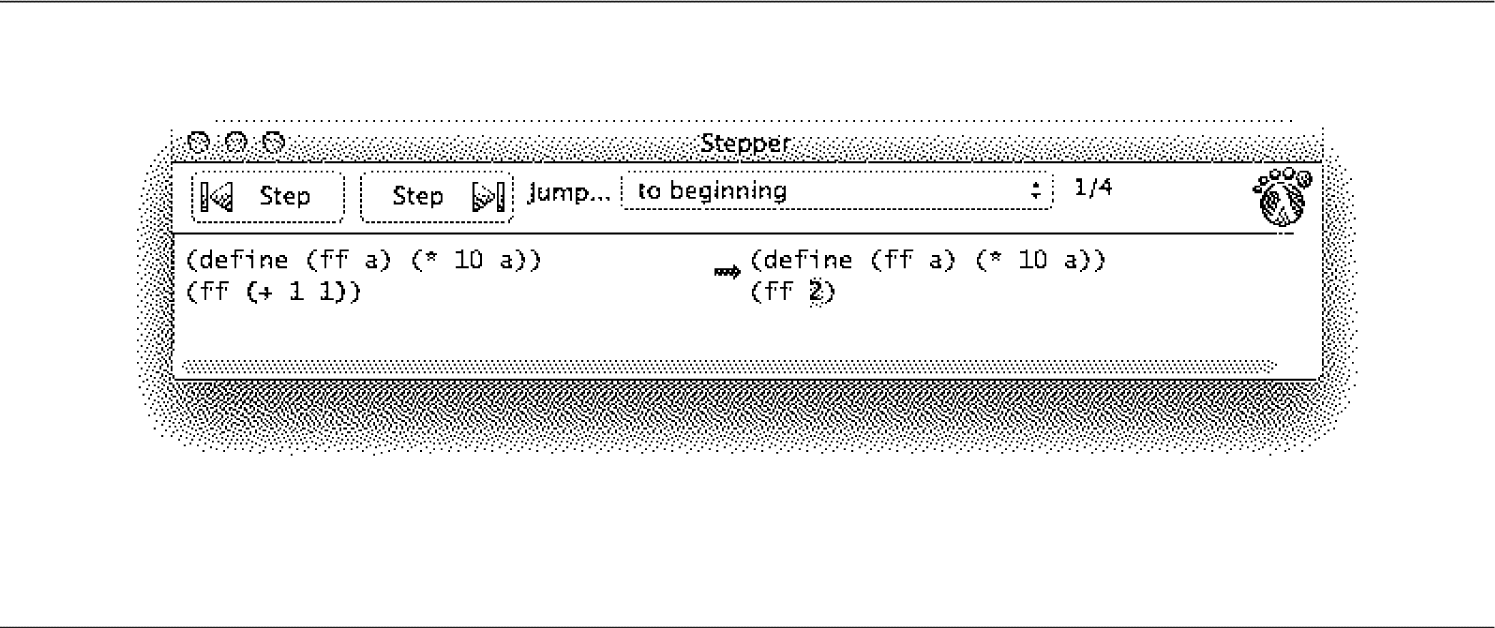
\includegraphics[width=0.75\textwidth]{images/00044.png}
  \caption{DrRacket 单步执行调试器（Stepper）}
  \label{fig:ch02_stepper}
\end{figure}

请停下来思考！是的，你完全可以用 DrRacket 来辅助检验你的代数作业。动手探索单步调试器提供的各种选项吧。

\begin{exercise}{利用单步调试器观察嵌套函数求值}{21}
在 DrRacket 中使用单步求值器逐步跟踪 \code{(ff (ff 1))} 的求值过程。然后再测试 \code{(+ (ff 1) (ff 1))}。仔细观察：DrRacket 的单步求值器会复用之前已经算好的子表达式计算结果吗？
\end{exercise}

此时此刻，你可能会觉得这与中学代数课没什么两样，尽是一些枯燥的数值与简单函数。但令人振奋的是，这一套“求值实参 $\rightarrow$ 变量代换 $\rightarrow$ 计算函数体”的计算法则，能够无缝推广到全书中所有令人惊艳的高级复杂程序！

我们来看看处理字符串的函数。回顾字符串的运算法则：
\begin{lstlisting}[language=BSL]
(string-append "hello" " " "world") == "hello world"
(string-append "bye" ", " "world")   == "bye, world"
\end{lstlisting}

现在假设我们定义一个生成信件开头的函数：
\begin{lstlisting}[language=BSL]
(define (opening first-name last-name)
  (string-append "Dear " first-name ","))
\end{lstlisting}

当给它传入两个字符串参数时，就能生成信件的称谓行：
\begin{replbox}
> (opening "Matthew" "Fisler")
"Dear Matthew,"
\end{replbox}

更为重要的是，计算法则清晰揭示了 DrRacket 是如何得出该结果的：
\begin{lstlisting}[language=BSL]
(opening "Matthew" "Fisler")
== ; 将 first-name 代换为 "Matthew"
(string-append "Dear " "Matthew" ",")
== "Dear Matthew,"
\end{lstlisting}
由于 \code{last-name} 未在函数体中被引用，用 \code{"Fisler"} 替换它不会产生任何额外影响。

本书后续章节将逐步介绍更多丰富的数据形态。而在解释各种数据上的操作时，我们始终如一地贯彻这种透明直观的代数计算法则。

\begin{notebox}[指令式操作前瞻]
在以后的高阶编程中，你可能会接触到“指令式操作”（imperative operations），它们不仅提取或组合数值，还会直接修改内存状态。要为这类操作推导演算，就需要在纯算术与代换法则之上引入额外的状态追踪机制。
\end{notebox}

\begin{exercise}{单步跟踪两点距离计算}{22}
在 DrRacket 中对以下程序片段启动单步求值器：
\begin{lstlisting}[language=BSL]
(define (distance-to-origin x y)
  (sqrt (+ (sqr x) (sqr y))))

(distance-to-origin 3 4)
\end{lstlisting}
单步求值器给出的每一步推导与你的直觉预期完全吻合吗？
\end{exercise}

\begin{exercise}{单步跟踪字符串首字符提取}{23}
字符串 \code{"hello world"} 的第一个 1String 是 \code{"h"}。下面的函数是如何计算出这一结果的？
\begin{lstlisting}[language=BSL]
(define (string-first s)
  (substring s 0 1))
\end{lstlisting}
使用单步求值器印证你的推导想法。
\end{exercise}

\begin{exercise}{单步跟踪逻辑蕴含函数求值}{24}
回顾练习~\ref{ex:15} 中逻辑蕴含函数 \code{==>} 的定义：
\begin{lstlisting}[language=BSL]
(define (==> x y)
  (or (not x) y))
\end{lstlisting}
使用单步求值器跟踪并确定表达式 \code{(==> \#true \#false)} 的一步步求值过程。
\end{exercise}

\begin{exercise}{通过单步调试修正图像分类函数}{25}
仔细研读下面这段试图解答练习~\ref{ex:17} 的初学者代码：
\begin{center}
  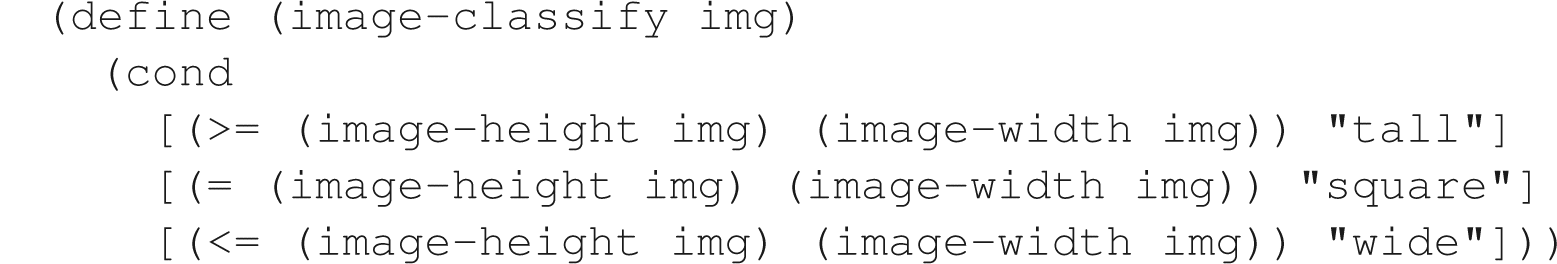
\includegraphics[width=0.8\textwidth]{images/00045.png}
\end{center}
在单步求值器中跟踪该函数在不同测试输入下的执行过程，你能发现代码中的缺陷并找到修复方案吗？
\end{exercise}

\begin{exercise}{单步跟踪复合字符串操作}{26}
在阅读并运行以下代码之前，先在脑海中预测它的执行结果：
\begin{center}
  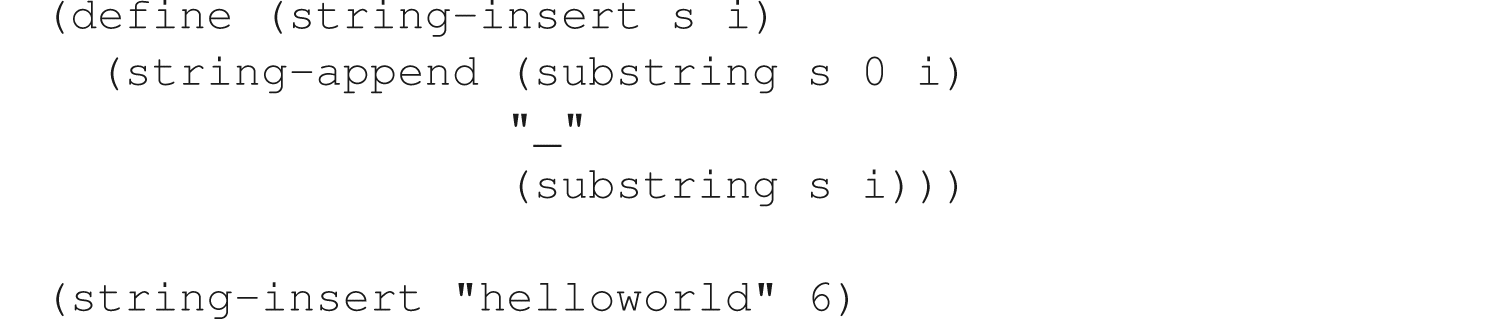
\includegraphics[width=0.7\textwidth]{images/00046.png}
\end{center}
随后在 DrRacket 中使用单步求值器验证你的预测。
\end{exercise}


% ==============================================================================
% 2.3 复合函数
% ==============================================================================
\section{复合函数}
\label{sec:2.3}

实际项目中的程序极少只由单个孤立的函数构成。典型的现代程序通常包含一个主函数和若干辅助函数，一个函数的输出往往顺畅流转为另一个函数的输入。与代数中的函数复合类比，我们将这种组织函数的方式称为\term{复合}（composition），这些协同工作的额外函数被称为\term{辅助函数}（auxiliary functions / helper functions）。

思考图~\ref{fig:ch02_batch_letter} 所示的信件模板生成程序。它由四个小函数有机协作构成：第一个是主函数 \code{letter}，它接收收件人的名、姓以及签名，生成一封完整格式的信件。主函数调用了三个辅助函数分别生成信件的三个独立部分（称谓行、正文段落和落款签名），最后通过 \code{string-append} 按正确顺序将各部分拼装合龙。

\begin{figure}[htbp]
  \centering
  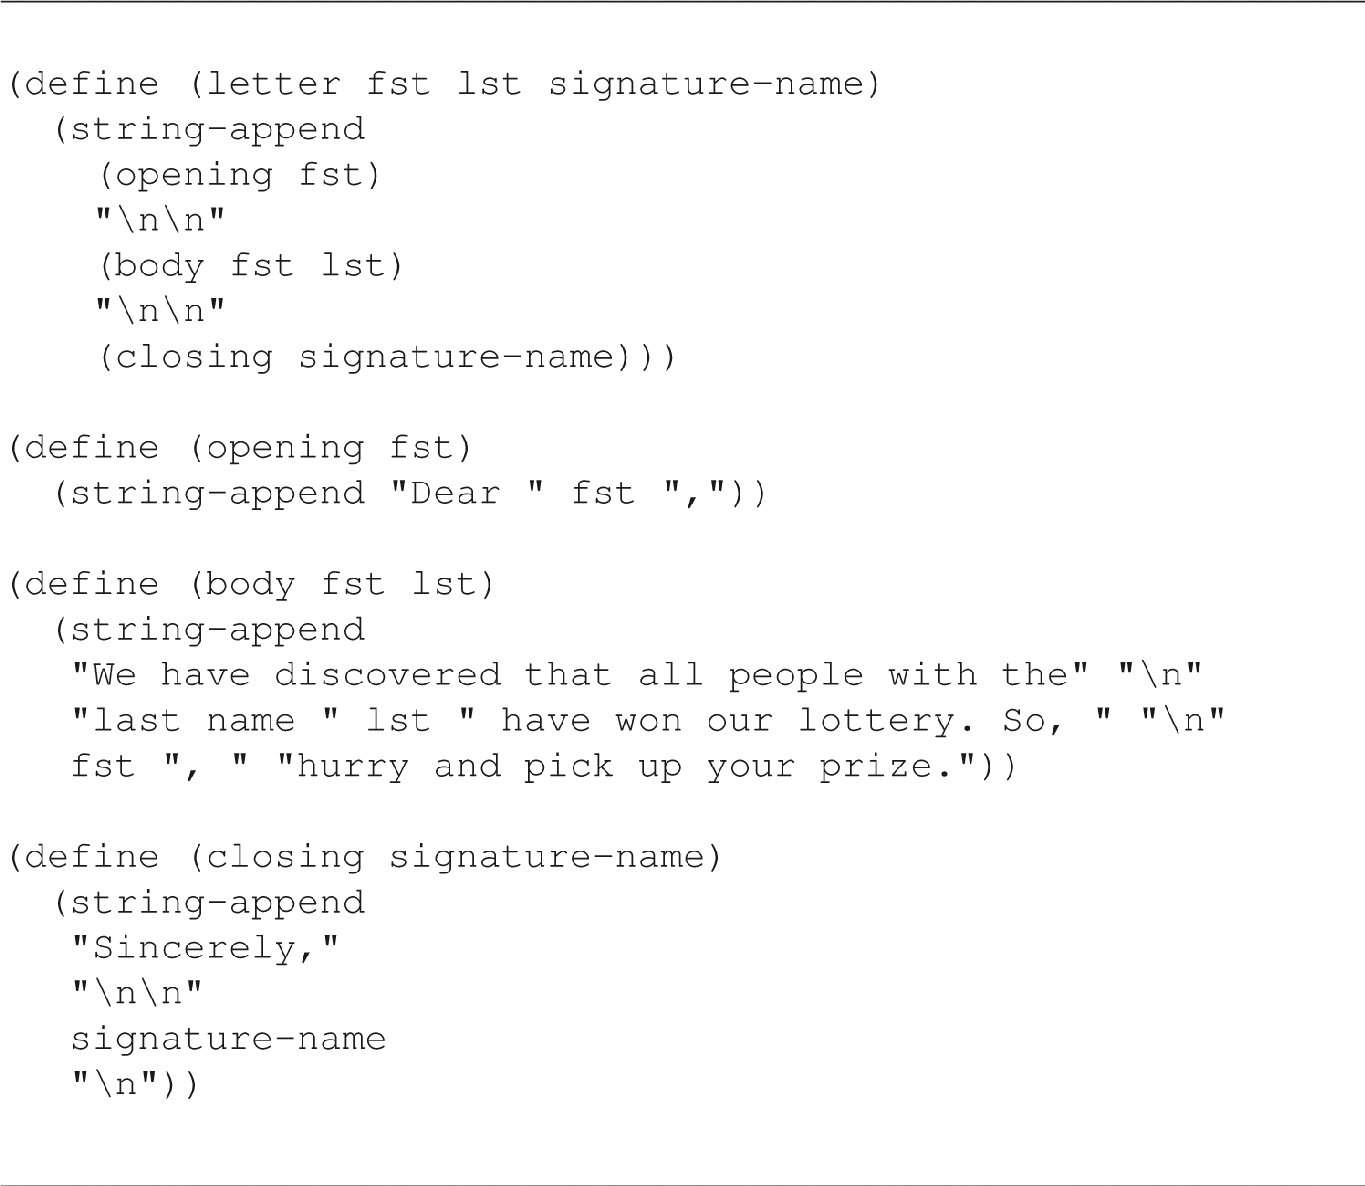
\includegraphics[width=0.85\textwidth]{images/00047.png}
  \caption{一个清晰模块化的批处理程序：信件生成器}
  \label{fig:ch02_batch_letter}
\end{figure}

请停下来思考！将上述定义输入 DrRacket 定义区，点击运行，然后在交互区中调用它们：
\begin{replbox}
> (letter "Matthew" "Fisler" "Felleisen")
"Dear Matthew,\n\nWe have discovered that ...\n"
> (letter "Kathi" "Felleisen" "Findler")
"Dear Kathi,\n\nWe have discovered that ...\n"
\end{replbox}

\begin{notebox}[控制台打印输出]
函数的返回值是一个包含换行符 \code{"\\n"} 的长字符串。如果在代码顶部加入 \code{(require 2htdp/batch-io)}，你的程序就能使用 \code{write-file} 函数，将格式化文本真实打印输出到控制台：
\begin{replbox}
> (write-file 'stdout (letter "Matt" "Fiss" "Fell"))
Dear Matt,

We have discovered that all people with the
last name Fiss have won our lottery. So,
Matt, hurry and pick up your prize.

Sincerely,
Fell
'stdout
\end{replbox}
目前可以把 \code{'stdout} 简单理解为一个代表“标准输出控制台”的特殊标记。第~2.5~节将详细剖析批处理程序。
\end{notebox}

面对一个包含多个明确计算子任务的实际问题，良好的程序架构应当贯彻黄金法则：\textbf{为每个子任务定义一个专门的函数，再由主函数统筹组装}。

\begin{notebox}[核心设计口诀]
\centering\Large\bfseries
每个任务定义一个函数\\
(Define one function per task)
\end{notebox}

遵循这一设计原则的巨大优势在于：你得到的每个小函数都足够精炼聚焦，其逻辑易于理解，它们之间的复合拓扑关系也清晰透明。一旦你掌握了科学的函数设计配方，就会深刻体会到：让一个小巧专注的函数正确工作，远比编写和调试一个庞大臃肿的巨石型函数轻松百倍！更有价值的是，当未来业务需求发生变更时，在由清晰小函数构建的模块化体系中定位并修改代码，犹如精准更换零件，比在数千行的单体代码中穿凿修改安全高效得多。

让我们通过一个经典的商业决策案例来体会这一原则的力量：

\begin{notebox}[案例研究：电影院最优票价决策]
某小镇上唯一的独家垄断电影院老板在设定电影票价时拥有完全的自主权。票价定得越高，能买得起票的观众就越少；票价定得越低，来看电影的人数就激增，但放映运营成本也随之上升。在近期的一项市场测试中，老板摸索出了票价与平均上座人数之间的精确函数关系：

当票价为每张 \$5.00 时，平均每场有 120 名观众；票价每变动 10 美分（\$0.10），平均上座人数就反向变动 15 人。也就是说，如果票价提高到 \$5.10，观众将减少到 105 人；若票价降至 \$4.90，观众将增加到 135 人。我们将这一市场规律转化为数学公式：
\[
  \text{avg.\ attendance} = 120\text{ people} - \frac{\$(\text{change in price})}{\$0.10} \cdot 15\text{ people}
\]
请停下来思考！在继续阅读之前，解释公式中减号的经济学含义。

然而，观众人数增加也会带来运营成本上升。每场放映包含 \$180 的固定运营成本，外加每位观众 \$0.04 的可变清洁服务成本。

影院老板急切想要知道：\textbf{净利润与票价之间的精确数学关系是什么？票价定在多少才能实现总利润最大化？}
\end{notebox}

虽然问题目标非常明确，但面对盘根错节的相互依赖关系，初学者往往不知从何下手。此时最佳的策略，就是贯彻口诀，将错综复杂的数量依赖关系逐一拆解为独立的纯函数：

\begin{enumerate}
  \item \textbf{上座人数依赖于票价}：计算观影人数显然是一个独立的业务规则，理应拥有专属的函数定义：
\begin{lstlisting}[language=BSL]
(define (attendees ticket-price)
  (- 120 (* (- ticket-price 5.0) (/ 15 0.1))))
\end{lstlisting}

  \item \textbf{总票房收入由售票产生}：总收入完全等于单张票价乘以观影人数：
\begin{lstlisting}[language=BSL]
(define (revenue ticket-price)
  (* ticket-price (attendees ticket-price)))
\end{lstlisting}

  \item \textbf{总放映成本由固定成本与可变成本构成}：由于观影人数本身是票价的函数，计算成本的函数同样接收票价作为参数，从而直接复用 \code{attendees} 函数：
\begin{lstlisting}[language=BSL]
(define (cost ticket-price)
  (+ 180 (* 0.04 (attendees ticket-price))))
\end{lstlisting}

  \item \textbf{最终净利润是总收入与总成本的差额}：
\begin{lstlisting}[language=BSL]
(define (profit ticket-price)
  (- (revenue ticket-price)
     (cost ticket-price)))
\end{lstlisting}
\end{enumerate}

\code{profit} 的 BSL 定义完全顺应了自然语言的问题陈述，清晰得如同一首代数诗篇！这四个各司其职的小函数共同构成了完整的利润核算程序，我们现在可以自由地在交互区中探寻最佳定价方案了。

\begin{exercise}{重构消灭魔法数：引入常量定义}{27}
我们在上面给出的示例代码中，函数体内部硬编码了许多“魔法数字”（magic numbers，例如 120、5.0、15、0.1、180、0.04 等）。正如序幕所强调的，赋予这些数字有意义的常量名称能够极大提升代码的可读性，让未来的维护者一眼看清数据来源。请将所有定义录入 DrRacket，并将所有魔法数重构为独立的全局常量定义。
\end{exercise}

\begin{exercise}{票价敏感度与影院利润最大化}{28}
使用 \code{profit} 函数分别计算票价为 \$1、\$2、\$3、\$4 和 \$5 时的潜在利润。哪一个整数票价能让影院利润最大化？在此基础上，进一步将票价精度精确到角（一角即 \$0.10），找出利润最丰厚的最佳票价。
\end{exercise}

作为对比，再看下面这个将所有计算步骤强行拼凑在单个函数体内部的“一体化单体版本”：
\begin{center}
  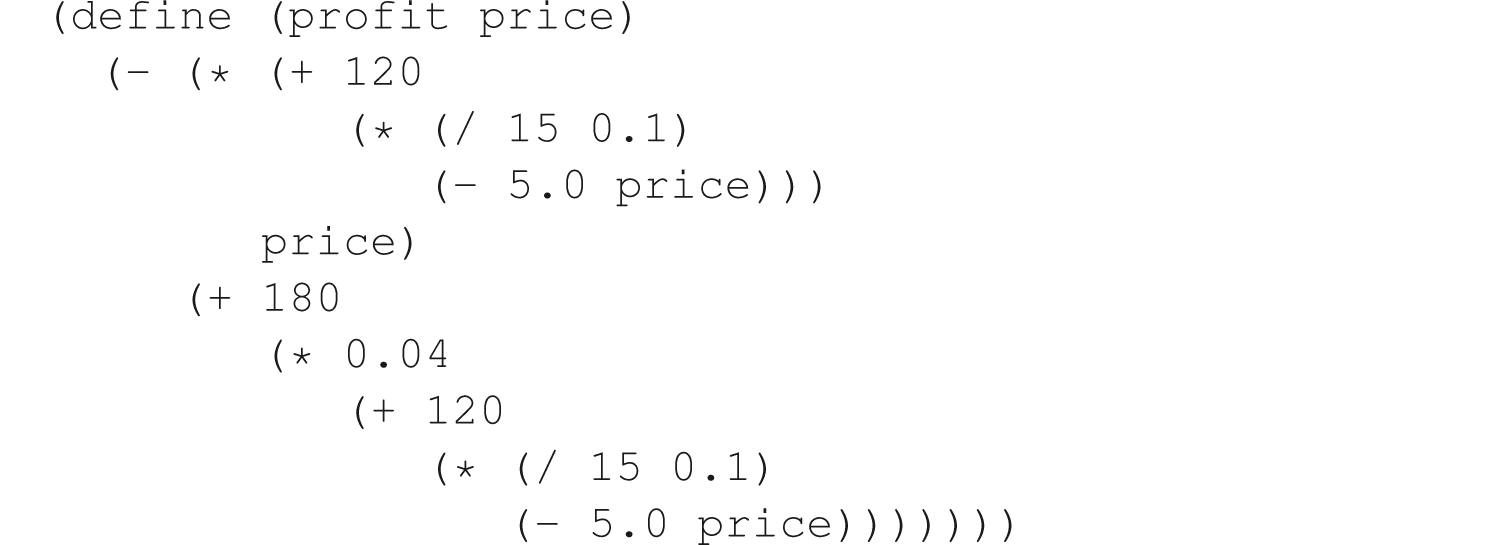
\includegraphics[width=0.85\textwidth]{images/00049.png}
\end{center}

将这个臃肿的单体函数输入 DrRacket，验证它在 \$1 到 \$5 票价下产生的结果确实与我们前面的模块化版本完全相同。但只需瞄上一眼，任何人都能立刻体会到：理解这个晦涩冗长的单体函数，比理解前面拆解明确的四个小巧函数要痛苦费力得多！

\begin{exercise}{电影院运营成本模型优化}{29}
在深入调研剧场日常开支后，老板找到了多种降低成本的有效途径。经过精益化改进后，固定放映成本被彻底削减为 0，而每位观众的可变服务成本调整为 \$1.50。

修改上述两种程序设计实现（模块化版本与单体版本）以反映这一商业规则变动。修改完成后，重新在 \$3、\$4 和 \$5 的票价下运行测试，对比两个版本的修改体验与计算结果。
\end{exercise}


% ==============================================================================
% 2.4 全局常量
% ==============================================================================
\section{全局常量}
\label{sec:2.4}

正如上文所示，类似 \code{profit} 这样的函数极大地受益于全局常量的抽取。任何完备的编程语言都允许开发者定义常量。在 BSL 中，常量定义遵循统一简洁的语法：
\begin{itemize}
  \item 写下 \code{(define}；
  \item 写下常量名称；
  \item 留出一个空格，写下一个表达式；
  \item 闭合右括号 \code{)}。
\end{itemize}

常量的名字是一个全局变量，而整条语句被称为常量定义。我们通常把常量定义中的表达式称为其“右侧表达式”（right-hand side）。

常量定义可以为任意形态的数据命名：数、图像、字符串等等。以下是一些典型示例：
\begin{lstlisting}[language=BSL]
; 当前电影票基准价格：
(define CURRENT-PRICE 5)

; 用于计算圆面积的近似圆周率：
(define ALMOST-PI 3.14)

; 换行符字符串：
(define NL "\n")

; 空白绘图背景画布：
(define MT (empty-scene 100 100))
\end{lstlisting}

前两个是数值常量，后两个分别是字符串常量和图像常量。按照工业界与函数式编程惯例，\textbf{全局常量通常采用大写字母命名}。这样可以保证无论代码库变得多么庞大，代码阅读者都能第一眼将全局常量与普通函数形参变量清晰地区分开来。

程序中的所有函数都可以自由引用这些全局变量。引用变量等同于直接使用对应的常量值。使用具名变量代替硬编码常量的最大好处在于：\textbf{一处修改，处处生效}。例如，我们想要提升圆周率的精度，或者放大画布的尺寸，只需修改一处定义：
\begin{lstlisting}[language=BSL]
(define ALMOST-PI 3.14159)
(define MT (empty-scene 200 800))
\end{lstlisting}
整个程序中所有依赖它们的地方都会自动同步更新。

我们不仅可以使用字面量来定义常量，还可以使用包含计算法则的复合表达式来定义\term{计算常量}（computed constants）：
\begin{lstlisting}[language=BSL]
(define WIDTH 100)
(define HEIGHT 200)
(define MID-WIDTH (/ WIDTH 2))
(define MID-HEIGHT (/ HEIGHT 2))
\end{lstlisting}
这里前两个常量采用字面量赋值，而后两个中心坐标常量则是通过对前两者进行代数计算得到的派生常量。

在此我们郑重提出第二条核心编程口诀：

\begin{notebox}[核心设计口诀]
\centering\Large\bfseries
问题陈述中提到的每一个常量，\\
都应为其引入一个常量定义！
\end{notebox}

\begin{exercise}{引入计算常量建模票价敏感度}{30}
为电影院最优票价程序定义一套完善的全局常量，使得“观众对票价的敏感度”（即每变动 10 美分增减 15 人）被重构为一个优雅的派生计算常量。
\end{exercise}


% ==============================================================================
% 2.5 程序
% ==============================================================================
\section{程序}
\label{sec:2.5}

现在，你已经完全具备了编写简单完整程序的全部基石！从代码构成来看，程序不过是一组函数定义与常量定义的有机集合。通常我们会明确指定一个主函数（main function），由它负责复合与调度其余辅助函数。然而从\textbf{程序启动与交互}的角度来看，软件世界主要分为两大截然不同的形态：
\begin{itemize}
  \item \term{批处理程序}（Batch Programs）：一次性接收全部输入数据，经内部管线计算后直接产出最终结果。其主函数是由辅助函数复合而成的管道。当启动批处理程序时，操作系统将输入传递给主函数，并静候其运算完成并输出。
  \item \term{交互式程序}（Interactive Programs）：以持续对话的方式运行，它消费部分输入，计算并输出部分结果，随后等待并响应新的外部输入。这种输入到达的时刻被称为\term{事件}（event），因此交互式程序本质上是\term{事件驱动程序}（event-driven programs）。这类程序的主函数通过配置明确告知操作系统：当特定类型的事件发生时，应当触发调用哪一个专属函数——这些函数被称为\term{事件处理器}（event handlers）。
\end{itemize}

当启动一个交互式程序时，主函数向宿主操作系统注册这份事件映射蓝图。每当输入事件发生，操作系统就调用匹配的事件处理器；同样，操作系统也会依据处理器的返回结果实时更新屏幕图像、播放声音等。

本书重点关注具有图形用户界面（GUI）的交互式程序；随着你继续深入探索计算机科学，你还会接触到基于网络套接字、传感器等多种形态的交互系统。

\subsection{批处理程序}

如前所述，批处理程序一次性消费所有输入数据，并由此计算出确定结果。其主函数接收参数，传递给底层辅助函数，收集各阶段的中间结果，最终整合成整体答案返回。

编写完成批处理程序后，我们可以在 DrRacket 交互区中手动调用主函数来观察其运作。而在工程实践中，更强大的用法是让程序直接从外部文件中读取数据，并将结果持久化写入新文件。历史上“批处理程序”这一称谓正源于早期计算机时代：打孔卡片被成批送入读卡机，程序读取整批卡片并在输出卡片上打孔记录结果。

通过引入 \code{2htdp/batch-io} 库，我们可以轻松构建基于文件的批处理程序：
\begin{itemize}
  \item \code{read-file}：将整个文件的文本内容一次性读取为一个字符串；
  \item \code{write-file}：接收一个目标文件名和一个字符串，将字符串完整写入该文件。
\end{itemize}

例如：
\begin{replbox}
> (write-file "sample.dat" "212")
"sample.dat"
> (read-file "sample.dat")
"212"
\end{replbox}

\begin{notebox}[文件路径安全提示]
在交互区执行读写文件命令前，请确保在 DrRacket 中先将定义区保存为一个实际的磁盘文件，以便确定相对路径基准。
\end{notebox}

执行第一句后，当前目录下会生成名为 \code{"sample.dat"} 的文件，内容为纯文本 \code{212}。\code{write-file} 返回文件名作为写入成功的确认；若文件已存在则会覆盖原有内容。第二句则把文件内容读取为字符串 \code{"212"}。

此外，\code{write-file} 还可以接收特殊符号 \code{'stdout}（标准输出设备）作为第一个参数，从而把文本直接打印在当前交互窗口中：
\begin{replbox}
> (write-file 'stdout "212\n")
212
'stdout
\end{replbox}
同理，\code{read-file} 也可以接收 \code{'stdin}（标准输入设备）从控制台交互区捕获用户键盘输入。

让我们通过一个温度换算程序来完整展示批处理程序的构建。假设我们要编写一个将华氏温度换算为摄氏温度的程序。物理换算公式如下：
\[
  C = \frac{5}{9} \cdot (f - 32)
\]
其中 $f$ 代表华氏度，$C$ 代表摄氏度。将这一公式翻译为 BSL 函数水到渠成：
\begin{lstlisting}[language=BSL]
(define (C f)
  (* 5/9 (- f 32)))
\end{lstlisting}
在交互区测试其计算精度：
\begin{replbox}
> (C 32)
0
> (C 212)
100
> (C -40)
-40
\end{replbox}

现在，我们希望将该核心算法封装进一个真正的批处理程序中：从指定文件读取华氏温度数值，进行换算，并将摄氏度结果写入输出文件。

\begin{center}
  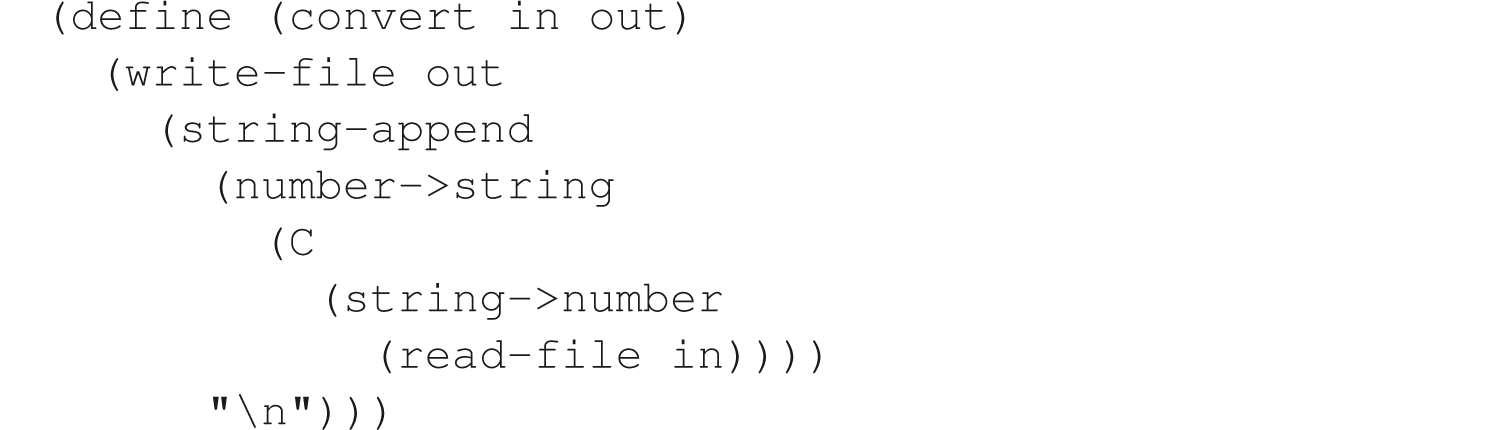
\includegraphics[width=0.85\textwidth]{images/00051.png}
\end{center}

主函数 \code{convert} 接收两个文件名参数：输入文件 \code{in} 与输出文件 \code{out}。它由 5 个函数无缝复合而成：
\begin{enumerate}
  \item \code{(read-file in)}：从输入文件读取全部内容为字符串；
  \item \code{string->number}：将该文本字符串解析为对应的数值；
  \item \code{C}：将该华氏数值精准转换为摄氏度数值；
  \item \code{number->string}：将计算出的摄氏度数值格式化为字符串；
  \item \code{(write-file out ...)}：将拼接好换行符的字符串最终落盘写入 \code{out} 文件。
\end{enumerate}

在交互区中实际测试该批处理管线：
\begin{replbox}
> (write-file "sample.dat" "212")
"sample.dat"
> (convert "sample.dat" 'stdout)
100
'stdout
> (convert "sample.dat" "out.dat")
"out.dat"
> (read-file "out.dat")
"100\n"
\end{replbox}

\begin{exercise}{运行信件生成批处理程序}{31}
回顾第~2.3~节的信件生成程序 \code{letter}。在交互区中针对至少三组不同的真实姓名调用 \code{letter} 并使用 \code{write-file} 输出到 \code{'stdout}。随后，利用下面的批处理函数，实现从三个独立文件读取姓名并生成信件文件：
\begin{center}
  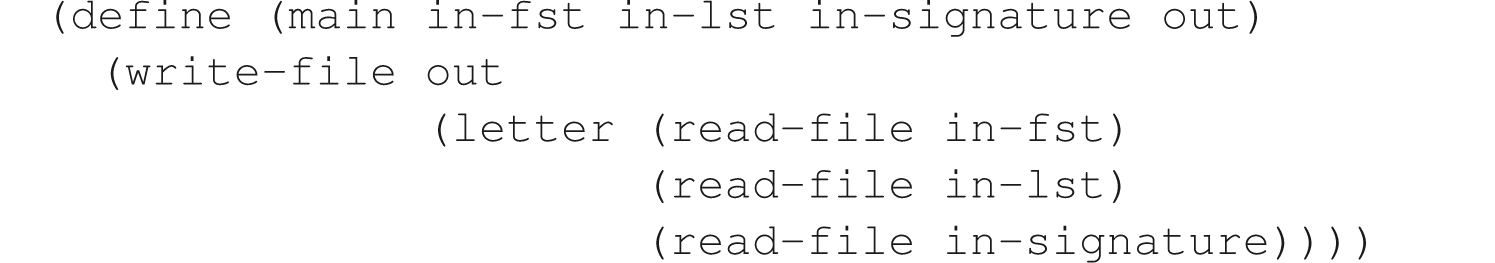
\includegraphics[width=0.85\textwidth]{images/00052.png}
\end{center}
创建输入文件，运行测试，并检查输出文件的内容。
\end{exercise}

\subsection{交互式程序}

批处理程序是商业后台计算的基石，但普通大众日常接触最多的则是图形交互软件。我们使用键盘和鼠标与桌面应用交流；此外，程序还必须时刻响应时钟跳动（clock ticks）或网络数据包到达等机器事件。

\begin{exercise}{未来交互式智能设备事件枚举}{32}
现代人不仅在台式机和笔记本上运行程序，智能手机、平板电脑和车载中控屏也已深度普及；未来更有智能眼镜、智能织物以及植入式生物芯片等新型计算形态。请列举出运行在这些前沿设备上的软件应用可能需要捕获并处理的 10 种不同形态的现实世界“事件”（events）。
\end{exercise}

孤立的计算机硬件只是一堆冰冷的物理电路。只有在安装了操作系统等系统软件后，它才具备生命力。当用户敲下键盘上的一个按键时，硬件中断会触发操作系统运行一段专门处理键盘敲击的例程。我们称这次按键为一个\term{按键事件}（key event），而处理它的函数就是\term{事件处理器}（event handler）。同理，时钟芯片每隔一定间隔发出滴答脉冲（clock tick），操作系统就执行一次时钟事件处理器。处理完毕后，系统调用渲染函数刷新显示屏像素。

面对千差万别的业务需求，不同程序需要注册不同的处理器：核电站控制程序与文字处理软件对按键的响应截然不同；火箭发射控制系统与微波炉定时软件对时钟脉冲的处理大相径庭。因此，设计一个交互式程序的核心任务，就是\textbf{向操作系统明确指定：哪一个函数负责处理键盘按键，哪一个函数负责处理时钟跳动，哪一个函数负责将程序当前状态绘制成可视图像}。

在 DrRacket 与 BSL 中，\code{2htdp/universe} 库提供的 \term{\code{big-bang}} 语法机制正是承担这一使命的指挥中枢！\code{big-bang} 负责追踪程序的当前\term{状态}（state）。它接收一个必选的初始状态表达式，以及一个必选的 \code{to-draw} 绘图子句，外加若干可选的事件监听子句。\code{to-draw} 告诉 DrRacket 如何把当前状态渲染为窗口图像；其余子句（如 \code{on-tick}、\code{on-key}、\code{on-mouse} 等）则分别指定各类事件的处理函数。

\begin{notebox}[世界程序 (World Programs) 术语]
在某种意义上，\code{big-bang} 表达式描述了程序所映射的一个微缩“世界”（World）的演进规则。这个微缩世界可能是一个贪吃蛇游戏、一个生动的物理动画，或者一个文本编辑器。因此，编程语言科学家常常将 \code{big-bang} 程序形象地称为\term{世界程序}（World Programs），并将程序的当前状态称为\term{世界状态}（State of the World）。
\end{notebox}

让我们从一个简单的绘图函数起步，逐步揭开 \code{big-bang} 的神奇面纱：
\begin{lstlisting}[language=BSL]
(define (number->square s)
  (square s "solid" "red"))
\end{lstlisting}
该函数接收一个正数，生成一个该边长的红色实心正方形。在交互区测试：
\begin{center}
  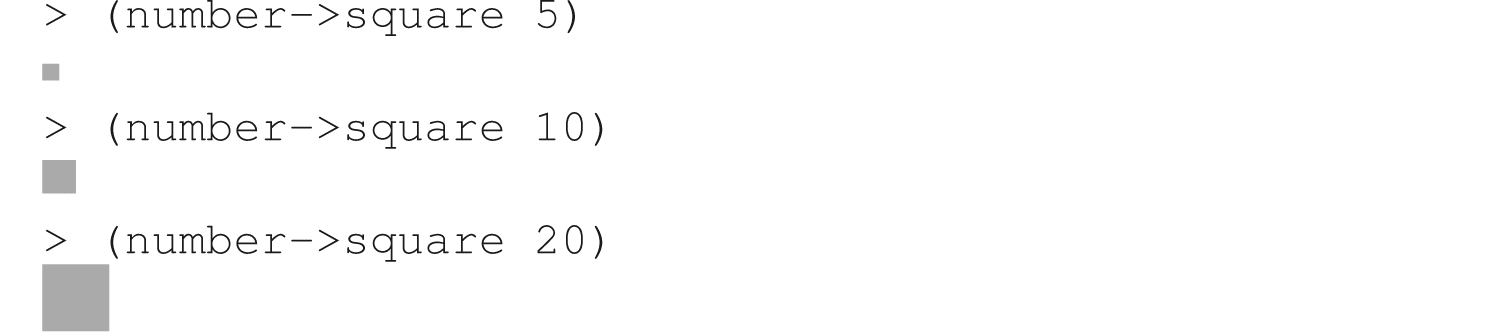
\includegraphics[width=0.7\textwidth]{images/00053.png}
\end{center}

现在在交互区输入最基础的 \code{big-bang} 表达式：
\begin{replbox}
> (big-bang 100 [to-draw number->square])
\end{replbox}

一个独立的画布窗口立即弹出，中央赫然显示出一个 $100 \times 100$ 的红色正方形！此时交互区并没有返回新的命令提示符，程序正在后台持续保持运行。点击窗口右上角的关闭按钮或 DrRacket 上的【停止】（STOP）按钮，程序终止并返回最终状态：
\begin{replbox}
100
\end{replbox}

现在看一个更加动感、功能丰富的 \code{big-bang} 表达式：
\begin{replbox}
> (big-bang 100
    [to-draw number->square]
    [on-tick sub1]
    [stop-when zero?])
\end{replbox}

这里添加了两个可选子句：\code{on-tick} 告诉系统每次时钟跳动时调用内置函数 \code{sub1}（当前值减 1）；\code{stop-when} 则指定当谓词 \code{zero?} 为真（即状态衰减到 0）时自动停止程序。整个生命周期如下：
\begin{enumerate}
  \item 初始状态为 100；
  \item 每当时钟跳动一次，当前状态减 1（经历 $100, 99, 98, \dots, 2, 1, 0$）；
  \item 每次状态发生改变，\code{to-draw} 调用 \code{number->square} 刷新窗口画面；
  \item 当状态变成 0 时，\code{stop-when} 触发，程序优雅终止并在交互区输出 0。
\end{enumerate}
你将亲眼目睹一个红色正方形在 100 个时钟周期内平滑缩小直至完全消失！

我们再进一步为它加上键盘响应能力。首先编写一个键盘事件处理函数：
\begin{lstlisting}[language=BSL]
(define (reset s ke)
  100)
\end{lstlisting}
该函数接收当前状态 \code{s} 和描述按键的字符串 \code{ke}，无条件重置返回 100。将它作为 \code{on-key} 挂载到 \code{big-bang} 中：
\begin{replbox}
> (big-bang 100
    [to-draw number->square]
    [on-tick sub1]
    [stop-when zero?]
    [on-key reset])
\end{replbox}

请停下来思考！按下回车启动程序，默数 10 秒，然后敲击键盘上的字母键 \code{"a"}，会发生什么奇妙的现象？

你会看到正方形正在一像素一像素地萎缩；然而一旦你敲下按键，\code{reset} 立即被触发并将状态重置为 100，正方形瞬间宛如充气般重新饱满膨胀到初始最大尺寸！

为了系统性地把握 \code{big-bang} 的全貌，图~\ref{fig:ch02_big_bang} 与下面的框架表达式完整展示了事件分发循环的内在逻辑：
\begin{lstlisting}[language=BSL]
(big-bang cw0
  [on-tick tock]
  [on-key ke-h]
  [on-mouse me-h]
  [to-draw render]
  [stop-when end?]
  ...)
\end{lstlisting}

\begin{figure}[htbp]
  \centering
  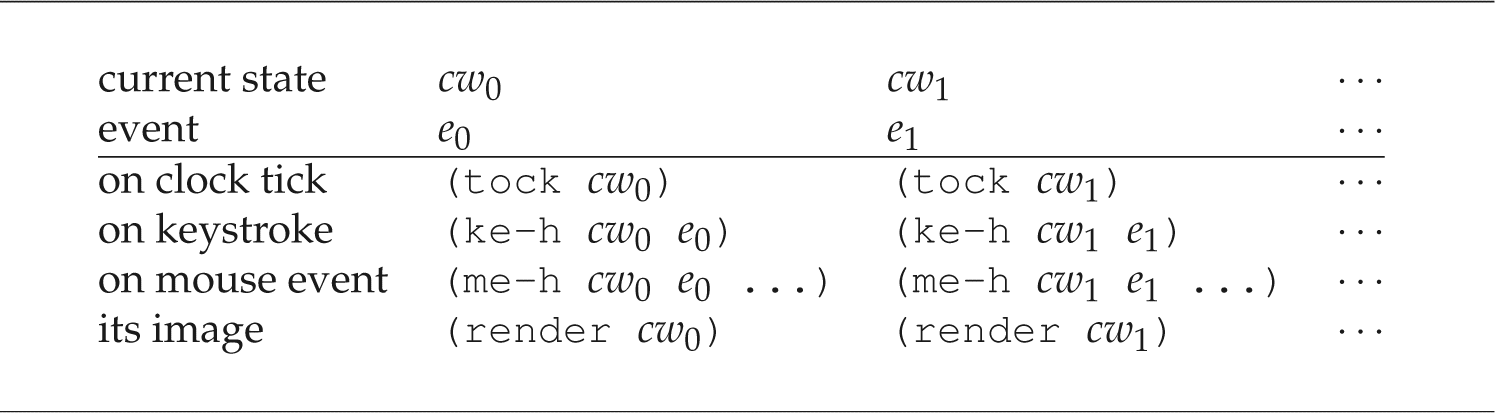
\includegraphics[width=0.95\textwidth]{images/00054.png}
  \caption{big-bang 交互式事件驱动引擎的工作机制}
  \label{fig:ch02_big_bang}
\end{figure}

事件循环的执行规则如下：
\begin{itemize}
  \item 系统以初始值 \code{cw0} 作为世界的当前状态（current world state）；
  \item 每次时钟脉冲到来，执行 \code{(tock cw)} 产出下一状态；
  \item 每次键盘敲击，执行 \code{(ke-h cw "按键名")} 产出下一状态；
  \item 每次鼠标移动或点击，执行 \code{(me-h cw x y "事件类型")} 产出下一状态；
  \item 任何事件处理完毕产生新状态后，系统首先执行 \code{(end? cw)} 检验是否应终止程序；若不终止，则调用 \code{(render cw)} 刷新屏幕图像。
\end{itemize}

图~\ref{fig:ch02_interactive_program} 给出了一个设计精巧、结构完整的第一个交互式世界程序范例：
\begin{figure}[htbp]
  \centering
  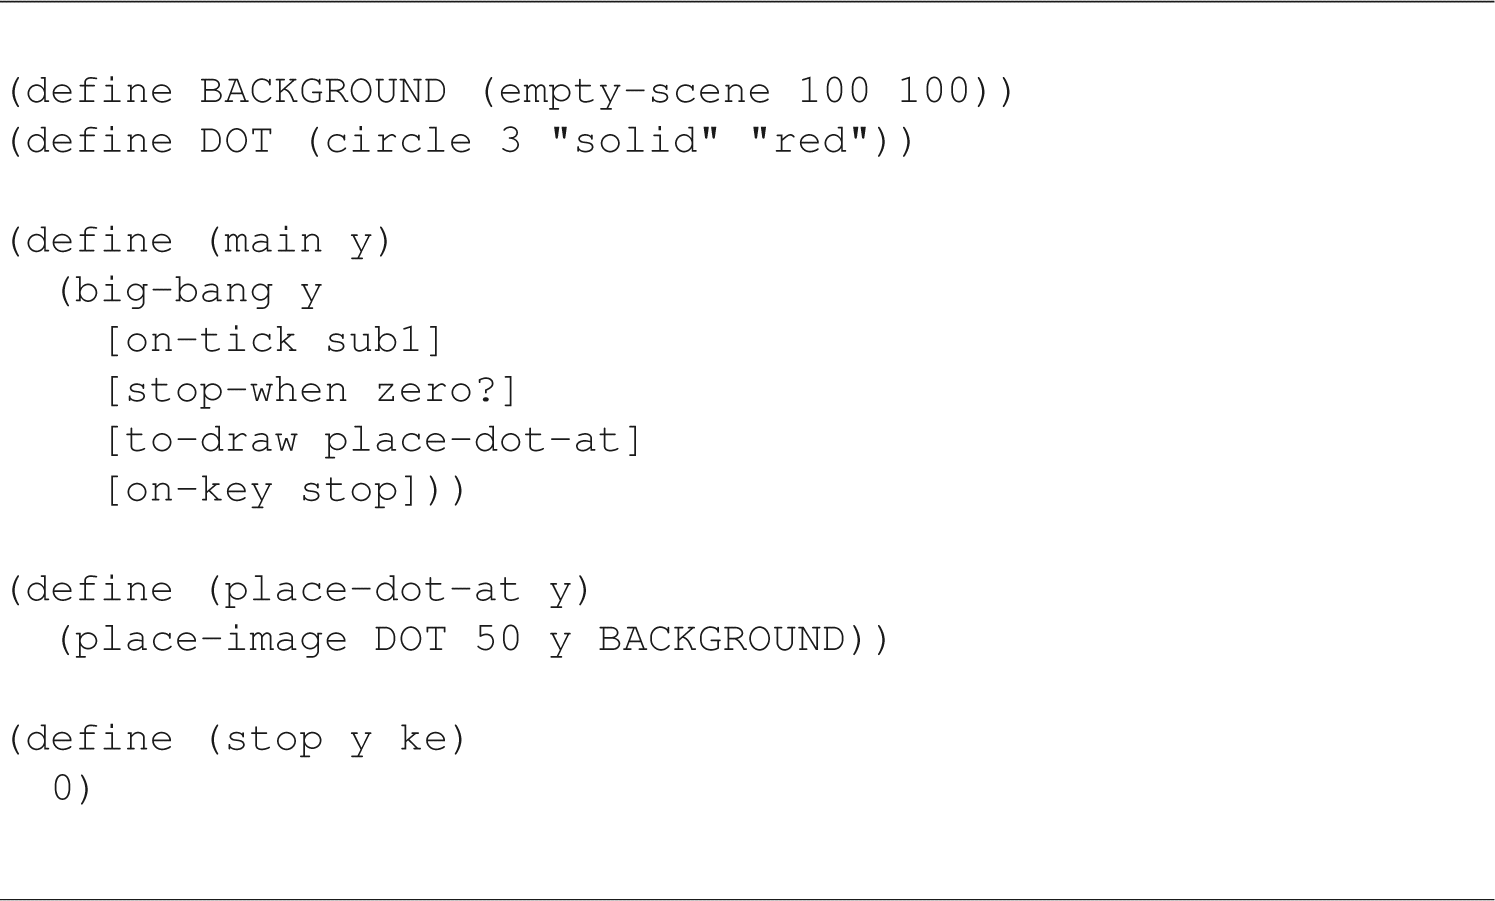
\includegraphics[width=0.85\textwidth]{images/00055.png}
  \caption{一个完整的初级交互式世界程序}
  \label{fig:ch02_interactive_program}
\end{figure}

在定义区输入该程序并点击运行，你可以在交互区中逐一调用它的各个处理函数进行独立单元验证：
\begin{center}
  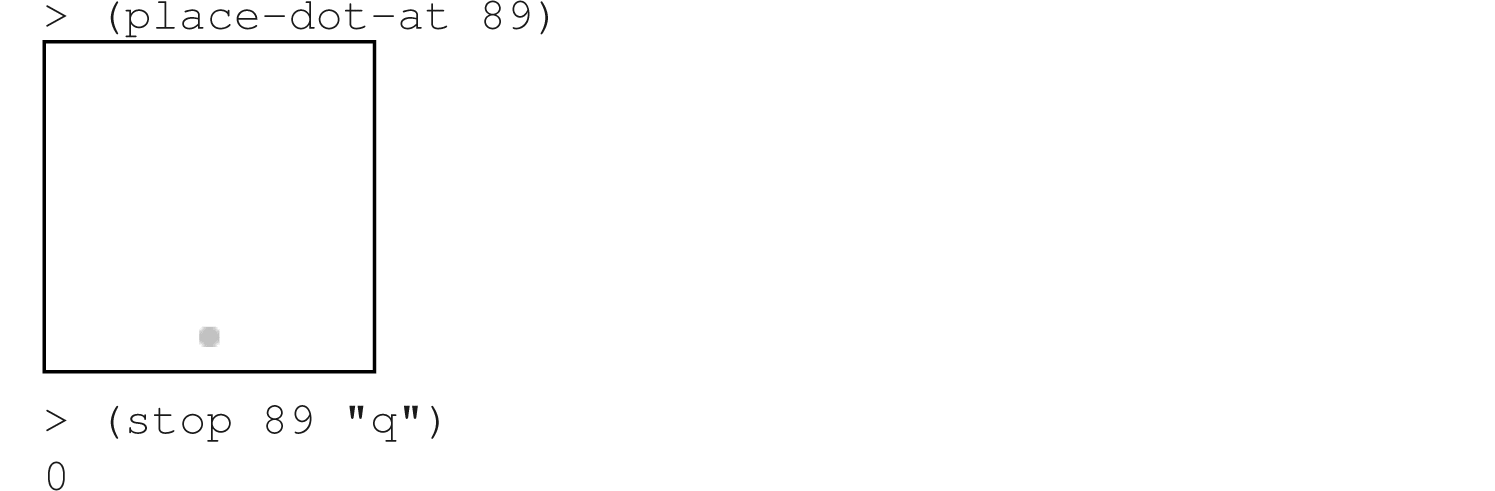
\includegraphics[width=0.75\textwidth]{images/00056.png}
\end{center}
随后调用 \code{(main 90)} 启动动画，亲手感受事件驱动编程的无穷魅力！

\vspace{1em}
\begin{notebox}[中途停歇与信心重塑]
读完前两章后，你可能会感到信息量巨大、有些应接不暇。我们学习了全新的 BSL 语言、前缀语法、求值规则、代数替换、常量规范、批处理以及基于 \code{big-bang} 的事件驱动机制。面对如此丰富的工具箱，当你拿到一个真实的问题陈述时，究竟该如何一步一个脚印地构思并设计出正确的程序呢？

别担心！下一章我们将放慢节奏，郑重为你揭晓全书的灵魂与精髓——\textbf{程序设计配方（Design Recipe）}。请稍事休息，准备迎接真正的编程思维蜕变！
\end{notebox}

% ==============================================================================
% 第 3 章：如何设计程序 (Chapter 3: How to Design Programs)
% ==============================================================================

\chapter{如何设计程序}
\label{sec:ch03_htdp}

本书前两章表明，学习编程需要掌握诸多核心概念。一方面，编程需要一门语言作为媒介，以此准确表达我们希望计算机执行的计算。用于表述程序的计算机语言是人工构建的符号系统，但掌握一门编程语言与掌握一门自然语言在很多方面有相通之处：二者都包含词汇、语法以及对“语句片段”所代表含义的理解。

另一方面，至关重要的是学会\textbf{如何从问题陈述一步步走向最终程序}。我们需要从自然语言的题目中辨别出哪些信息是关键核心，哪些细节可以暂时忽略；我们需要抽丝剥茧，理清程序接收什么输入、产出什么输出，以及输入与输出之间存在怎样的对应规律；我们需要了解并确认所选用的语言及其内置库是否已经提供了处理这些数据所需的基础操作——若未提供，我们必须有能力构思并实现相应的辅助函数；最后，当代码写完后，我们必须严格检验它是否确实完成了预期的计算，并在发现各色各样的缺陷时，能够从容理解并修复它们。

所有这一切听起来颇具挑战，你可能会纳闷：为什么我们不直接“摸着石头过河”，随性写写改改、到处试试，只要凑出看起来还不错的输出结果就收工大吉？这种常被称为“车库式编程”（garage programming）的随性方式极为普遍，且在许多场合确能取得暂时的成功；它甚至往往是许多初创公司的起步摇篮。然而，初创公司绝无法直接将这种粗糙的“车库产物”作为可靠产品推向市场，因为除了最初的作者及其亲近的朋友，外人根本无法理解、使用和维护它。

一个优秀的程序必须配备简明扼要的说明文档，清晰阐述它的功能职责、期望接收的输入类型以及产出的输出规格。理想情况下，它还应自带一套可自动验证其正确性的证据体系。在最理想的工程状态下，程序代码与原始问题陈述之间的映射关系应当一目了然，从而使业务需求上的微小变动能够轻而易举地映射为程序代码中的微小调整。软件工程师将这种严谨的工业级成品称为\term{编程产品}（programming product）。

这一切看似额外的严谨工作之所以不可或缺，是因为\textbf{程序员从来不是只为自己写代码}。程序员写出的代码是给其他程序员阅读的，而在特定的时刻，人们会运行这些代码来解决现实问题。绝大多数现实程序都是由成百上千个函数协同协作的庞大系统，没有任何人能在一天之内独立写完所有模块。工程师加入项目团队、编写代码、随后离开；新的维护者接手遗留系统并继续演进。另一个无法回避的现实是：客户对业务需求的理解往往是动态变化的，他们最初提出的需求通常只说对了大半，细节上往往错漏频出。更糟糕的是，程序作为高度复杂的逻辑构造体，不可避免地会受到人类思维盲区的影响——简言之，程序员必定会犯错。终有一天，潜在的缺陷会暴露出来，工程师必须回过头来，重新研读一个月前、一年前、甚至二十年前写下的代码并进行修正。

\begin{notebox}[重读代码的现实]
这里所说的“其他程序员”，也包括“未来的你自己”——数月之后的你通常早已记不清当初年轻的自己在编写这段代码时脑海中的全部推导细节。
\end{notebox}

\begin{exercise}{千年虫（Y2K）问题调研}{33}
通过查阅资料，调研 20 世纪末震惊全球的“2000 年问题”（又称千年虫问题，Y2K problem）。了解当时的程序员为何采用两位数字来表示年份，以及这一历史设计决策在数十年后给全球银行业、航空业及各工业系统造成了何种深远的技术与经济冲击。
\end{exercise}

为了帮助所有人摆脱盲目摸索的泥潭，我们在此隆重推出\term{程序设计配方}（Design Recipe）。它将系统化的分步推导过程与以问题数据为核心的程序组织结构紧密熔铸为一体。对于那些一面对着空白屏幕就陷入焦虑发呆的读者，这套设计配方提供了一条有章可循、步步为营的确定性路径；对于从事编程教学的教师，它是诊断初学者思维卡点的精准试金石；对于从事医学、新闻或工程等其他领域的专业人士，这套科学严谨的问题解决范式同样能够跨界迁移；而对于立志成为一流软件架构师的读者，设计配方更是深入剖析并驾驭现有复杂大型软件的无上利器。

本章的剩余部分将带你迈出踏入设计配方世界的第一步；在后续各章节与各部分中，我们将在此基础上不断对该配方进行迭代深化与拓展。


% ==============================================================================
% 3.1 设计函数
% ==============================================================================
\section{设计函数}
\label{sec:3.1}

\subsection{信息与数据}

程序的终极目的，是描述一个消费现实\term{信息}（information）并产出全新信息的计算过程。从这个意义上说，程序类似于数学老师向小学生布置的解题指令。但与学生不同的是，程序处理的对象远不仅限于数字：它计算导航路线、检索联系人地址、操控物理开关、或者维护电子游戏的世界状态。所有这些信息均来源于现实世界的某一特定领域——通常被称为程序的\term{业务领域}（domain），而程序计算产出的成果则代表了该领域中的新信息。

“信息”在我们的设计哲学中居于中枢地位。可以将信息视为关于程序业务领域的具体事实。对于一个家具目录管理系统，“五条腿的桌子”或“两米乘两米的正方形桌子”都是信息。游戏程序面向不同的业务领域，其中的数值“5”可能代表游戏角色在屏幕上每个时钟周期移动的像素位移。而在薪资结算系统中，“5”可能代表“五项税前扣除”。

为了让程序能够处理现实信息，它首先必须将信息转化为编程语言内部的某种\term{数据}（data）；随后对这些数据执行计算；计算完毕后再将产出的数据还原解释为现实信息。对于交互式程序，这三步可能交替穿插、往复循环：根据需要随时从外部世界捕获更多新信息，并在计算间隙持续向现实世界反馈信息。

我们之所以选用 BSL 语言与 DrRacket 环境，正是为了让你在起步阶段完全不必为“信息与数据之间复杂的底层编解码”分心劳神。在 DrRacket 中，你可以直接把函数应用到核心数据上并直接观察其产出。这样就巧妙避开了“既要写业务计算、又要写复杂数据解析器”的鸡生蛋蛋生鸡困境。对于简单形态的信息，编写转换代码尚属简单；但对于复杂信息，你需要深入掌握语法解析（parsing）等高阶技术，而这需要非常扎实的程序设计功底作为前提。

软件工程界常用\term{模型--视图--控制器}（MVC）这一经典架构模式来概括这种分离：BSL 与 DrRacket 将底层纯数据处理与外部界面的信息解析和呈现彻底解耦。现代高质量软件工程已经形成共识：优秀的系统必须严格执行这种分层解耦，哪怕许多入门书籍仍然将二者混为一谈。依托 BSL 和 DrRacket，你可以心无旁骛地专注于程序核心计算逻辑的设计；当你在核心设计上积累了足够的经验之后，再自如地进阶学习信息与数据双向转换的专门技术。

图~\ref{fig:ch03_info_data} 形象地揭示了从现实信息到计算机数据、再由计算数据还原为现实信息的完整认知闭环。

\begin{figure}[htbp]
  \centering
  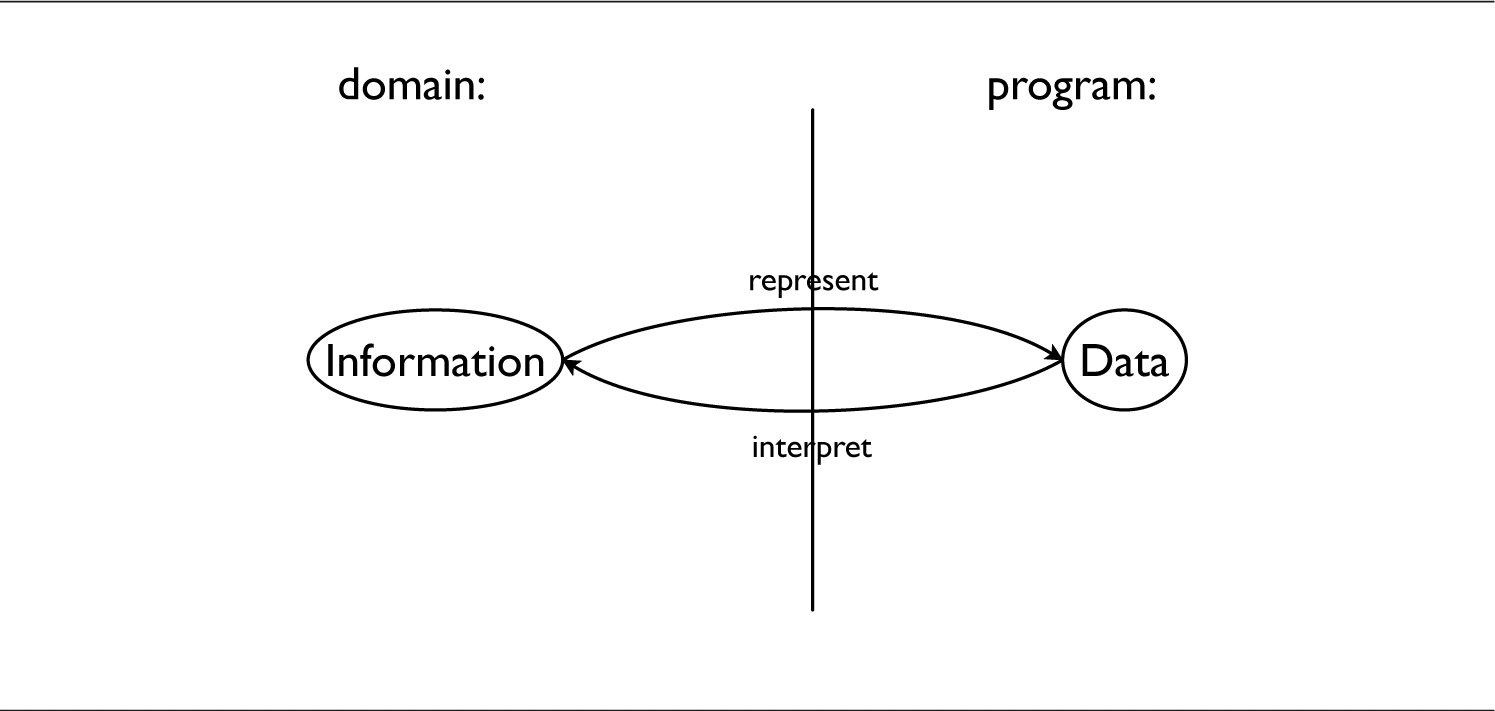
\includegraphics[width=0.75\textwidth]{images/00057.png}
  \caption{从现实领域信息到计算机数据，再由数据还原为领域信息}
  \label{fig:ch03_info_data}
\end{figure}

为了让这一核心概念生动具体，让我们考察几个现实场景。假设你正在设计一个以数值形式接收和产出信息的程序。尽管在计算机中选用数字作为底层数据表示极其简单，但如何\textbf{诠释}（interpretation）这些数据——即说明数值 42 在现实领域中到底代表什么——才是关键所在：
\begin{itemize}
  \item 在图像排版领域，42 可能代表距离画布顶端边界的像素偏移量；
  \item 在物理模拟或游戏世界中，42 可能代表动画精灵每个时钟周期移动的像素速率；
  \item 在气象物理领域，42 可能代表摄氏度、华氏度或开尔文温标下的测量温度；
  \item 在家具商城的库存系统中，42 可能代表某款餐桌的定制规格尺寸；
  \item 或者，42 仅仅代表某个文本字符串中的字符总数。
\end{itemize}
设计的精髓，就在于清晰掌握如何在现实信息与程序数据之间建立严谨、准确的双向映射桥梁。

鉴于这种认知映射对于每一位代码阅读者都至关重要，我们在代码中通过注释的形式将其明确记录下来，这被称为\term{数据定义}（data definitions）。数据定义承担着两大核心使命：
\begin{enumerate}
  \item 使用具有明确业务含义的词汇为某一类数据集合命名（赋予其一个数据类型名称）；
  \item 清晰告知代码阅读者如何创建属于该集合的有效数据，以及如何判断任意一个给定数据是否属于该数据类。
\end{enumerate}

\begin{notebox}[数据类 (Class)]
计算机科学家在这里使用“类”（Class）一词，其含义等同于数学中的“集合”（Set）。
\end{notebox}

下面是上述温度案例的一个规范数据定义示例：
\begin{lstlisting}[language=BSL]
; 一个 Temperature（温度）是一个 Number（数）。
; 诠释：代表摄氏度数值
\end{lstlisting}

第一行引入了该数据集合的专用名称 \code{Temperature}，并指明该类由全体数值（Number）构成。因此，当我们询问 102 是否是一个 Temperature 时，你可以笃定地回答“是”，因为 102 是一个数；同理，若问 \code{"cold"} 是否属于 Temperature，答案显然是“否”，因为字符串绝不属于数值。如果你被要求给出一个合法的 Temperature 样例，你可能会随手写出 $-400$。

如果你恰好掌握物理常识，知道现实宇宙中的理论最低温度（绝对零度）约为 $-273.15^\circ\text{C}$，你可能会好奇：我们能否在数据定义中精确表达这种物理现实约束？答案是完全可以！既然数据定义本质上是用严谨文本对数据集合的规范约定，你尽可以使用更精准的限制条件来定义温度。在接下来的章节中，我们将正式引入规范的区间与约束标记风格，例如“大于 $-273.15$ 的数”。

到目前为止，你已经见过了四种基础数据大类：\code{Number}、\code{String}、\code{Image} 以及 \code{Boolean}。在现阶段，制定一个新的数据定义，往往只是为已有的原生数据形态赋予一个贴合具体业务情境的新名字（例如将数值命名为温度）。即便仅凭这一点，也足以支撑起一套完整的函数设计配方。

\subsection{函数设计配方的六大步骤}

一旦明确了如何将输入的领域信息表示为计算机数据、以及如何将输出数据诠释为现实信息，设计单个函数的全过程就归纳为一套清晰、严密、环环相扣的标准配方：

\begin{recipebox}{函数设计配方 (Design Recipe for Functions)}
\begin{enumerate}
  \item \textbf{数据表示与数据定义 (Data Definition)}：明确现实信息如何表示为程序数据，写下核心数据定义与诠释注释。
  \item \textbf{签名、目的说明与函数头 (Signature, Purpose Statement, Header)}：
    \begin{itemize}
      \item \textbf{签名}（Signature）：指明函数消费什么类型的输入，产出什么类型的输出；
      \item \textbf{目的说明}（Purpose Statement）：用一两句话精炼阐释该函数计算的目标；
      \item \textbf{函数头 / 桩函数}（Header / Stub）：用形参变量搭建函数雏形，给出占位返回值。
    \end{itemize}
  \item \textbf{功能示例 (Functional Examples)}：根据签名选取典型输入，先于编码手工推导出预期的正确输出。
  \item \textbf{盘点资产与模板 (Inventory and Template)}：依据输入数据特征搭建函数体逻辑骨架，明确计算时可用的全部输入资产。
  \item \textbf{编写代码 (Coding)}：用具体的代数计算表达式填充模板，兑现目的说明中所承诺的业务契约。
  \item \textbf{自动化测试 (Testing)}：将先前的功能示例转化为可执行的单元测试，彻底验证函数的正确性。
\end{enumerate}
\end{recipebox}

让我们逐一深入剖析这六大步骤的具体实操：

\paragraph{第 1 步：数据表示与数据定义}
用单行注释或规范格式清晰声明数据表示方法。例如：
\begin{lstlisting}[language=BSL]
; 我们使用数（Number）表示以厘米为单位的长度。
\end{lstlisting}
为你认为对程序成功至关重要的核心概念拟定正式的数据定义。

\paragraph{第 2 步：签名、目的说明与函数头}
\term{函数签名}（Signature）是一条指引代码阅读者的核心注释，它清晰罗列了函数接收几个输入、这些输入分别来自哪些数据类、以及最终产出的数据属于什么类型。例如：
\begin{lstlisting}[language=BSL]
; String -> Number
; 接收一个字符串，产出其字符长度数值

; Temperature -> String
; 接收一个温度值，产出其状态描述文本

; Number String Image -> Image
; 接收一个数、一个字符串和一张图像，产出一张全新合成的图像
\end{lstlisting}

\term{目的说明}（Purpose Statement）是用简洁的一两行注释回答最本质的问题：\textbf{这个函数究竟计算出什么？} 任何阅读你代码的人，都应当无需通读复杂函数体，仅凭目的说明就能彻底洞悉函数的计算意图。

\term{函数头}（Header）又常被称为\term{桩函数}（Stub）：它确定函数名称，为签名中的每一个输入类别选取一个有意义的形参变量名，并在函数体中填入输出类别的任意一个默认字面量：
\begin{lstlisting}[language=BSL]
(define (f a-string) 0)
(define (g n) "a")
(define (h num str img) (empty-scene 100 100))
\end{lstlisting}
在编写目的说明时，善于利用形参变量名往往能让表达格外精准：
\begin{lstlisting}[language=BSL]
; Number String Image -> Image
; 将文字 s 绘制为图像并叠加到 img 上，
; 距顶部 y 像素，距左边缘 10 像素
(define (add-image y s img)
  (empty-scene 100 100))
\end{lstlisting}
至此，你已经可以点击【运行】按钮，语法检查会顺利通过。

\paragraph{第 3 步：功能示例}
通过列举具体生动的输入输出用例，来具象化签名和目的说明。从输入的合法数据集中挑选几个典型值，亲手计算出预期的正确答案：
\begin{lstlisting}[language=BSL]
; Number -> Number
; 计算边长为 len 的正方形的面积
; 给定输入: 2, 期望输出: 4
; 给定输入: 7, 期望输出: 49
(define (area-of-square len) 0)
\end{lstlisting}

\paragraph{第 4 步：梳理资产与模板}
在动手写实现之前，必须先\term{梳理已有资产}（take inventory，即盘点可用输入与组件）：我们手头拥有的已知输入是什么？需要计算出的目标又是什么？对于基础函数，所有已知数据均通过参数传入。为了时刻提醒自己这一核心事实，我们将桩函数中的虚拟默认值替换为一个包含所有形参变量的\term{模板}（template）：
\begin{lstlisting}[language=BSL]
(define (area-of-square len)
  (... len ...))
\end{lstlisting}
省略号 \code{(...)} 明确提醒你：这还不是一个能跑的代码，而是一张指明可用原料的结构图纸。

\paragraph{第 5 步：编写代码}
在 HtDP 体系中，所谓的“编码”（coding），就是用符合计算逻辑的具体表达式替换模板中的省略号，利用梳理出的已知参数与可用组件，彻底兑现目的说明中所许下的承诺：
\begin{lstlisting}[language=BSL]
; Number -> Number
; 计算边长为 len 的正方形的面积
; 给定: 2, 期望: 4
; 给定: 7, 期望: 49
(define (area-of-square len)
  (sqr len))
\end{lstlisting}
对于略复杂的函数（例如前文提到的 \code{add-image}），完成这一步需要组合多层图形绘制函数，如图~\ref{fig:ch03_step5} 所示。

\begin{figure}[htbp]
  \centering
\begin{lstlisting}[language=BSL, basicstyle=\scriptsize\ttfamily]
; Number String Image -> Image
; adds s to img, y pixels from top, 10 pixels to the left
; given:
;     5 for y,
;     "hello" for s, and
;     (empty-scene 100 100) for img
; expected:
;     (place-image (text "hello" 10 "red") 10 5 ...)
;     where ... is (empty-scene 100 100)
(define (add-image y s img)
  (place-image (text s 10 "red") 10 y img))
\end{lstlisting}
  \caption{函数设计第 5 步（编码兑现）的完成形态}
  \label{fig:ch03_step5}
\end{figure}

\paragraph{第 6 步：测试}
严谨设计的收尾之笔，是使用之前第 3 步列出的功能示例，对编写好的函数展开无情检验。点击运行，在交互区逐一验证：
\begin{replbox}
> (area-of-square 2)
4
> (area-of-square 7)
49
\end{replbox}

如果实际结果与预期完全一致，函数设计大功告成！若发生偏差，通常有三种可能原因：
\begin{enumerate}[label=(\alph*)]
  \item 你在第 3 步手工演算时粗心算错了预期值；
  \item 函数体代码编写有误，即程序存在逻辑缺陷（Bug）；
  \item 示例预期值与函数实现双双出现错误。
\end{enumerate}
排查时，应首先重新核验示例预期值的正确性；一旦确认示例无误，则全力排查函数体逻辑。


% ==============================================================================
% 3.2 基础练习：函数
% ==============================================================================
\section{基础练习：函数}
\label{sec:3.2}

接下来的几道基础练手习题与第~2.1~节中的练习题目高度相似，但请注意关键措辞的变化：第~2.1~节使用的是“定义”（define），而这里的要求全部是“\textbf{设计}”（design）！这意味着你必须\textbf{严格走完设计配方的全部六个步骤}，你的最终解答必须完整包含：数据定义、签名、目的说明、功能用例、模板及最终测试！

正如本节标题所示，这些练习是为了帮助你将设计配方内化为本能肌肉记忆。在这些步骤彻底变成你的第二本能之前，切勿跳过任何一步。编程世界中不乏极其深奥复杂的逻辑难题，我们绝不需要在低级疏忽上无谓浪费精力。

\begin{exercise}{设计提取首字符函数 string-first}{34}
严格按照设计配方，设计函数 \code{string-first}：从一个非空字符串中提取出它的第一个字符。暂时无需考虑空字符串的情况。
\end{exercise}

\begin{exercise}{设计提取尾字符函数 string-last}{35}
严格按照设计配方，设计函数 \code{string-last}：从一个非空字符串中提取出它的最后一个字符。
\end{exercise}

\begin{exercise}{设计计算图像面积函数 image-area}{36}
严格按照设计配方，设计函数 \code{image-area}：计算并返回给定图像所占据的像素总数（宽 $\times$ 高）。
\end{exercise}

\begin{exercise}{设计删除首字符函数 string-rest}{37}
严格按照设计配方，设计函数 \code{string-rest}：接收一个字符串，产出删除了首字符之后的其余字符串片段。
\end{exercise}

\begin{exercise}{设计删除尾字符函数 string-remove-last}{38}
严格按照设计配方，设计函数 \code{string-remove-last}：接收一个字符串，产出删除了末尾字符之后的其余字符串片段。
\end{exercise}


% ==============================================================================
% 3.3 领域知识
% ==============================================================================
\section{领域知识}
\label{sec:3.3}

初学者常会好奇：究竟需要具备怎样的知识储备，才能顺利写出函数体中的计算表达式？稍加审视便不难发现，这高度依赖于程序员对程序\term{业务领域}（domain）的认知深度。具体来说，领域知识主要来自两大方面：
\begin{enumerate}
  \item \textbf{外部应用领域的专业知识}：如数学、音乐、生物、土木建筑、金融或艺术等。程序员不可能通晓人类所有的行业学科，因此必须具备敏锐的跨界学习能力，能够听懂各行业专家的专业行话，并与之展开高密度的严谨讨论。数学往往是绝大多数理工领域的通用交集，但在更多交叉领域中，程序员必须边干边学。
  \item \textbf{所选编程语言及其标准库知识}：当任务涉及三角函数时，你需要知道 BSL 已经内置了 \code{tan}；当任务涉及图形绘制与动画渲染时，熟悉 \code{2htdp/image} 库的丰富接口将让你事半功倍。
\end{enumerate}

由于你永远无法预料未来会被委派去解决哪个领域的难题、或者必须使用哪一门编程工具，因此对可用计算工具箱的全貌建立清晰扎实的把握是生死攸关的。否则，那些略懂皮毛脚本的业务人员就会轻易取代你的位置。

通过审视设计配方第 1 步拟定的数据定义，你通常能一眼判断出该问题对领域知识的依赖程度：只要数据定义使用的是编程语言已经原生支持的数据形态，函数体的编写主要考验的是业务领域专业素养；而当我们在后文引入复杂自建数据结构时，程序设计的核心就转变为纯粹的计算机科学专业技能。


% ==============================================================================
% 3.4 从函数到程序
% ==============================================================================
\section{从函数到程序}
\label{sec:3.4}

真正的工程程序几乎不可能只由单体函数构成。大型系统不仅包含多重嵌套的函数网络，还包含广泛的全局常量定义。但无论软件系统多么宏大，系统化设计每一个基础函数的铁律绝不可动摇。

当你引入了全局常量后，各个函数都可以自由调用这些常量来计算结果。为了时刻提醒自己这些外部常量的存在，你可以把它们一并列入第 4 步的“资产盘点与模板”中作为可用资产。

多函数协作体系在交互式程序中表现得尤为明显：事件驱动系统天然需要专门处理键盘的函数、专门处理时钟的函数、以及负责图形渲染的视图函数。而在批处理程序中，拆分独立计算任务同样需要多个辅助函数的协同。这些子任务的需求，有时在阅读问题陈述之初就已浮出水面，有时则是在设计某一主函数的过程中中途顿悟发现的。

为此，我们强烈建议每一位开发者在纸上或代码注释中维护一张\term{愿望清单}（Wish List）。愿望清单上的每一个待实现条目均包含三项要素：
\begin{itemize}
  \item 一个见名知意的函数名称；
  \item 严谨清晰的函数签名；
  \item 简练的目的说明。
\end{itemize}

在设计批处理程序时，先将主函数放入愿望清单并开始攻坚；在设计交互式世界程序时，可将各个事件处理器、终止判断函数及场景渲染函数率先挂在愿望清单上。只要清单非空，就从中挑出一个愿望，运用六步设计配方彻底兑现它。如果在设计过程中发现需要新的辅助函数，立即将其追加到清单末尾。当清单上的所有愿望都被一一实现之时，整个程序便宣告完美竣工！


% ==============================================================================
% 3.5 关于测试
% ==============================================================================
\section{关于测试}
\label{sec:3.5}

手动执行测试很快就会沦为令人心力交瘁的苦力活。在交互区手工输入函数调用虽然直观，但要求肉眼反复校对复杂的数值或长文本。随着系统规模不断扩充，每次修改代码后都需要回归检验成百上千个用例，手动测试很快就会不堪重负，以至于程序员开始心存侥幸地怠慢测试。然而，严谨测试是捕捉并扑灭初级逻辑缺陷的第一道钢铁防线。马虎敷衍的测试必将迅速导致隐蔽 Bug 在代码库中潜伏滋生，最终全方位拖垮工程进度。

因此，\textbf{将测试全面自动化是现代软件工程的立身之本}！BSL 原生内置了极其优雅的自动化测试框架，DrRacket 会在后台全力保障其高效运行。让我们以华氏度转摄氏度的经典函数为例：
\begin{lstlisting}[language=BSL]
; Number -> Number
; 将华氏温度转换为摄氏温度
; 给定 32, 期望 0
; 给定 212, 期望 100
; 给定 -40, 期望 -40
(define (f2c f)
  (* 5/9 (- f 32)))
\end{lstlisting}

为了测试该函数，我们需要进行三次代数计算以及三次数值等值比较。在 BSL 中，你可以直接使用 \term{\code{check-expect}} 语法将其声明在定义区中：
\begin{lstlisting}[language=BSL]
(check-expect (f2c -40) -40)
(check-expect (f2c 32) 0)
(check-expect (f2c 212) 100)
\end{lstlisting}

现在只需轻轻点击【运行】按钮，DrRacket 就会自动运行并向你回报：\textbf{全套测试用例 100\% 全部通过！} 无需任何人工肉眼比对，省心省力！

当测试未通过时，\code{check-expect} 的威力表现得更为惊艳。假设我们故意在测试中引入一个错误断言：
\begin{lstlisting}[language=BSL]
(check-expect (f2c -40) 40)
\end{lstlisting}
再次点击运行，DrRacket 立即弹出一个专用的测试报告浮窗，清晰指出：3 个测试中有 1 个未通过，并以醒目的高亮对照列出：实际计算值（$-40$）、期望断言值（$40$），并附带可一键直达出错测试源码的超链接！

\code{check-expect} 既可以写在函数定义之后，也可以直接写在函数定义之前。点击运行后，DrRacket 会先预先加载所有函数定义，随后集中统一执行所有测试。如图~\ref{fig:ch03_testing} 所示，我们可以把设计配方的第 3 步（功能示例）与第 6 步（测试）合二为一：\textbf{直接用 \code{check-expect} 写出示例用例}。编写代码的同时就构筑好了测试护栏，未来对函数的任何微小修改，只需点击一次运行就能瞬间完成自动化回归验证。

\begin{figure}[htbp]
  \centering
\begin{lstlisting}[language=BSL, basicstyle=\scriptsize\ttfamily]
; Number -> Number
; converts Fahrenheit temperatures to Celsius temperatures

(check-expect (f2c -40) -40)
(check-expect (f2c 32) 0)
(check-expect (f2c 212) 100)

(define (f2c f)
  (* 5/9 (- f 32)))
\end{lstlisting}
  \caption{在 BSL 中运用 check-expect 构建自动化单元测试}
  \label{fig:ch03_testing}
\end{figure}

更令人拍案叫绝的是，\code{check-expect} 对图像对象完全原生支持！这意味着你可以直接对产出图像的视图函数展开像素级的精确断言。例如我们要设计小车渲染函数 \code{render}：
\begin{center}
  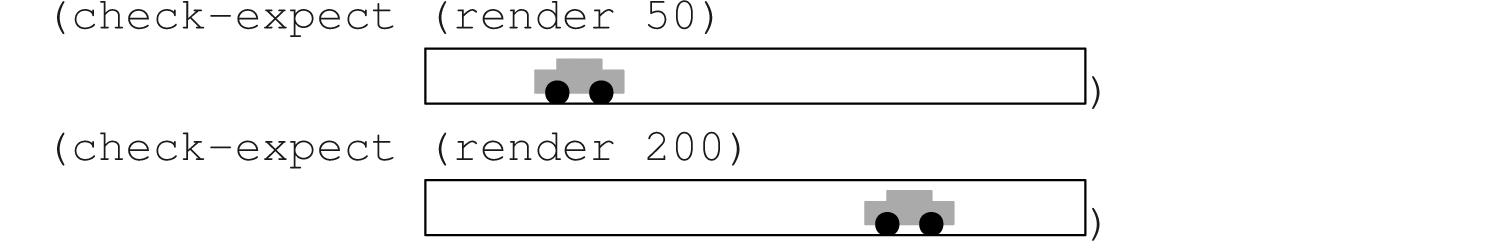
\includegraphics[width=0.85\textwidth]{images/00060.png}
\end{center}
或者，也可以使用绘图公式进行测试断言：
\begin{lstlisting}[language=BSL, basicstyle=\scriptsize\ttfamily]
(check-expect (render 50)
              (place-image CAR 50 Y-CAR BACKGROUND))
(check-expect (render 200)
              (place-image CAR 200 Y-CAR BACKGROUND))
\end{lstlisting}
后一种方式还能反哺指导我们推导函数体的具体实现逻辑。

这种由系统自动执行、针对独立软件组件开展的自动化测试机制被称为\term{单元测试}（Unit Testing）。在本书后续的所有章节中，我们将全面普及这种规范的测试实践。未来当你切换到其他主流编程语言时，你最先应该探索的也正是其对应的单元测试框架。


% ==============================================================================
% 3.6 设计世界程序
% ==============================================================================
\section{设计世界程序}
\label{sec:3.6}

前一章我们以探索性的方式介绍了 \code{2htdp/universe} 库；本节我们将展示如何将设计配方全面升华，系统化指导交互式“世界程序”的架构与设计。

世界程序库的核心运作理念非常清晰：开发者需要拟定一套代表整个“世界状态”的数据定义，以及一个能将任意世界状态绘制为可视画面的渲染函数 \code{render}。随后，根据应用需求设计响应时钟周期的 \code{tock}、响应键盘的 \code{key-handler} 以及响应鼠标的 \code{mouse-handler}；若需要在满足特定条件时退出，还需设计判定终止的谓词 \code{end?}。图~\ref{fig:ch03_wish_list} 给出了设计世界程序时标准的初始愿望清单蓝图。

\begin{figure}[htbp]
  \centering
\begin{lstlisting}[language=BSL, basicstyle=\scriptsize\ttfamily]
; WorldState: data that represents the state of the world (cw)

; WorldState -> Image
; when needed, big-bang obtains the image of the current
; state of the world by evaluating (render cw)
(define (render ws) ...)

; WorldState -> WorldState
; for each tick of the clock, big-bang obtains the next
; state of the world from (clock-tick-handler cw)
(define (clock-tick-handler cw) ...)

; WorldState String -> WorldState
; for each keystroke, big-bang obtains the next state
; from (keystroke-handler cw ke); ke represents the key
(define (keystroke-handler cw ke) ...)

; WorldState Number Number String -> WorldState
; for each mouse gesture, big-bang obtains the next state
; from (mouse-event-handler cw x y me) where x and y are
; the coordinates of the event and me is its description
(define (mouse-event-handler cw x y me) ...)

; WorldState -> Boolean
; after each event, big-bang evaluates (end? cw)
(define (end? cw) ...)
\end{lstlisting}
  \caption{设计交互式世界程序的通用初始愿望清单}
  \label{fig:ch03_wish_list}
\end{figure}

让我们通过一个生动的实战案例来完整演练这套设计配方：

\begin{notebox}[案例实战：小车水平匀速行驶]
\textbf{问题陈述}：设计一个动画世界程序，使一辆小车在画布场景中从左向右持续平移，每经历一个时钟周期向右移动 3 个像素。
\end{notebox}

对于这个场景，我们可以直观勾勒出不同时刻的世界画面：
\begin{center}
  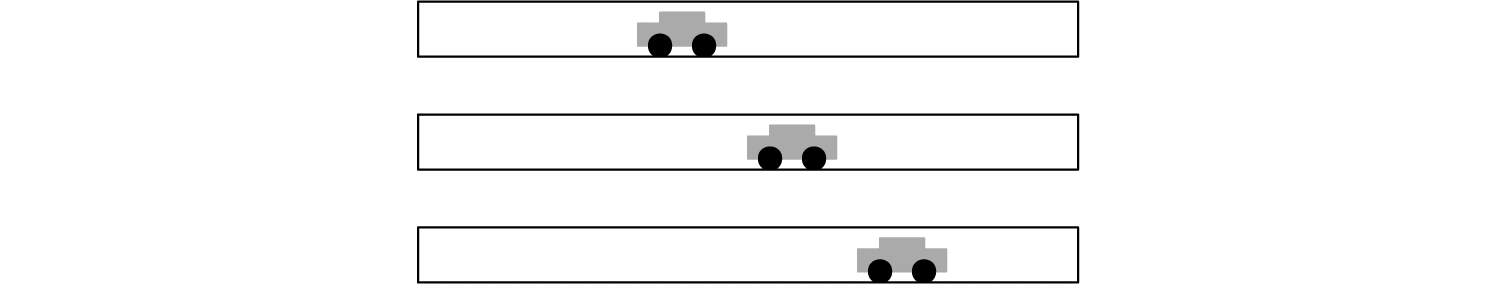
\includegraphics[width=0.85\textwidth]{images/00063.png}
\end{center}

世界程序的设计配方包含三大核心阶段外加一个装配步骤：

\begin{recipebox}{世界程序设计配方 (Design Recipe for World Programs)}
\begin{enumerate}
  \item \textbf{界定并提取全局常量}：
    \begin{itemize}
      \item \textbf{物理常量}：描述世界中物体的固有属性（运动速度、宽高、车轮半径等）；
      \item \textbf{图形常量}：在画布上静态呈现的各种基础视觉元素（车轮、车身、树木、背景等）。
    \end{itemize}
  \item \textbf{确立世界状态的数据表示 (WorldState)}：辨识随着时间推移、受事件驱动而动态改变的核心属性，为其拟定精确的数据定义与业务诠释。
  \item \textbf{逐一兑现愿望清单上的各个处理函数}：
    \begin{itemize}
      \item 必备的场景渲染函数 \code{render : WorldState -> Image}；
      \item 按需设计时钟、键盘、鼠标事件处理器及终止判定谓词。
    \end{itemize}
  \item \textbf{编写主启动函数 (main)}：将初始状态与各事件子句装配进 \code{big-bang} 表达式中。
\end{enumerate}
\end{recipebox}

\paragraph{第一步：常量抽取与单点控制原则}
在小车行进世界中，小车运动速率、画布长宽以及车轮间距是恒定不变的“物理常量”：
\begin{lstlisting}[language=BSL]
(define WIDTH-OF-WORLD 200)
(define WHEEL-RADIUS 5)
(define WHEEL-DISTANCE (* WHEEL-RADIUS 5))
\end{lstlisting}

进而，我们可以通过代数运算由物理常量派生构建小车的各部分“图形常量”：
\begin{lstlisting}[language=BSL]
(define WHEEL (circle WHEEL-RADIUS "solid" "black"))
(define SPACE (rectangle ... WHEEL-RADIUS ... "white"))
(define BOTH-WHEELS (beside WHEEL SPACE WHEEL))
\end{lstlisting}

\begin{exercise}{单点控制原则与汽车图像缩放}{39}
优秀的软件架构师会确保像 \code{CAR} 这样的复杂图形常量能够通过修改单个底层基准常量来实现全局等比缩放。我们在构建小车时以车轮半径为基准：
\begin{lstlisting}[language=BSL]
(define WHEEL-RADIUS 5)
\end{lstlisting}
所有车轮间距、车身长宽、车顶弧度均以此为依据派生计算。这样一来，将 \code{WHEEL-RADIUS} 从 5 改为 10，整辆小车就会全局自适应等比放大一倍。这种卓越的工程规范被称为\term{单点控制原则}（single point of control）。请设计并绘制一辆你喜欢的小汽车图像，确保 \code{WHEEL-RADIUS} 是控制其尺寸的唯一控制源。
\end{exercise}

\paragraph{第二步：世界状态数据定义}
在动画播放过程中，动态演变的是小车相对于场景左边界的距离。距离可以用非负数值精确刻画，因此我们写下清晰的数据定义：
\begin{lstlisting}[language=BSL]
; 一个 WorldState 是一个 Number。
; 诠释：代表小车距离画布左边界的像素位移量
\end{lstlisting}

\paragraph{第三步：愿望清单与函数设计}
根据业务规则，我们需要一个时钟处理器 \code{tock}（每次时钟周期小车右移 3 像素）和一个渲染函数 \code{render}：
\begin{lstlisting}[language=BSL]
; WorldState -> WorldState
; 每次时钟滴答，将小车横坐标加 3
(check-expect (tock 20) 23)
(check-expect (tock 78) 81)
(define (tock ws)
  (+ ws 3))
\end{lstlisting}

\begin{exercise}{将样例改写为 BSL 自动化测试}{40}
将上述 \code{tock} 函数的示例在 DrRacket 中编写为完整的 \code{check-expect} 测试。故意在测试中制造一个计算偏差，观察自动化测试窗口的报错交互反馈；随后将其修正并重新运行。
\end{exercise}

接下来设计视图渲染函数 \code{render}。我们可以通过图~\ref{fig:ch03_car_examples} 中的对照表格来直观归纳函数体的构造规律：
\begin{figure}[htbp]
  \centering
  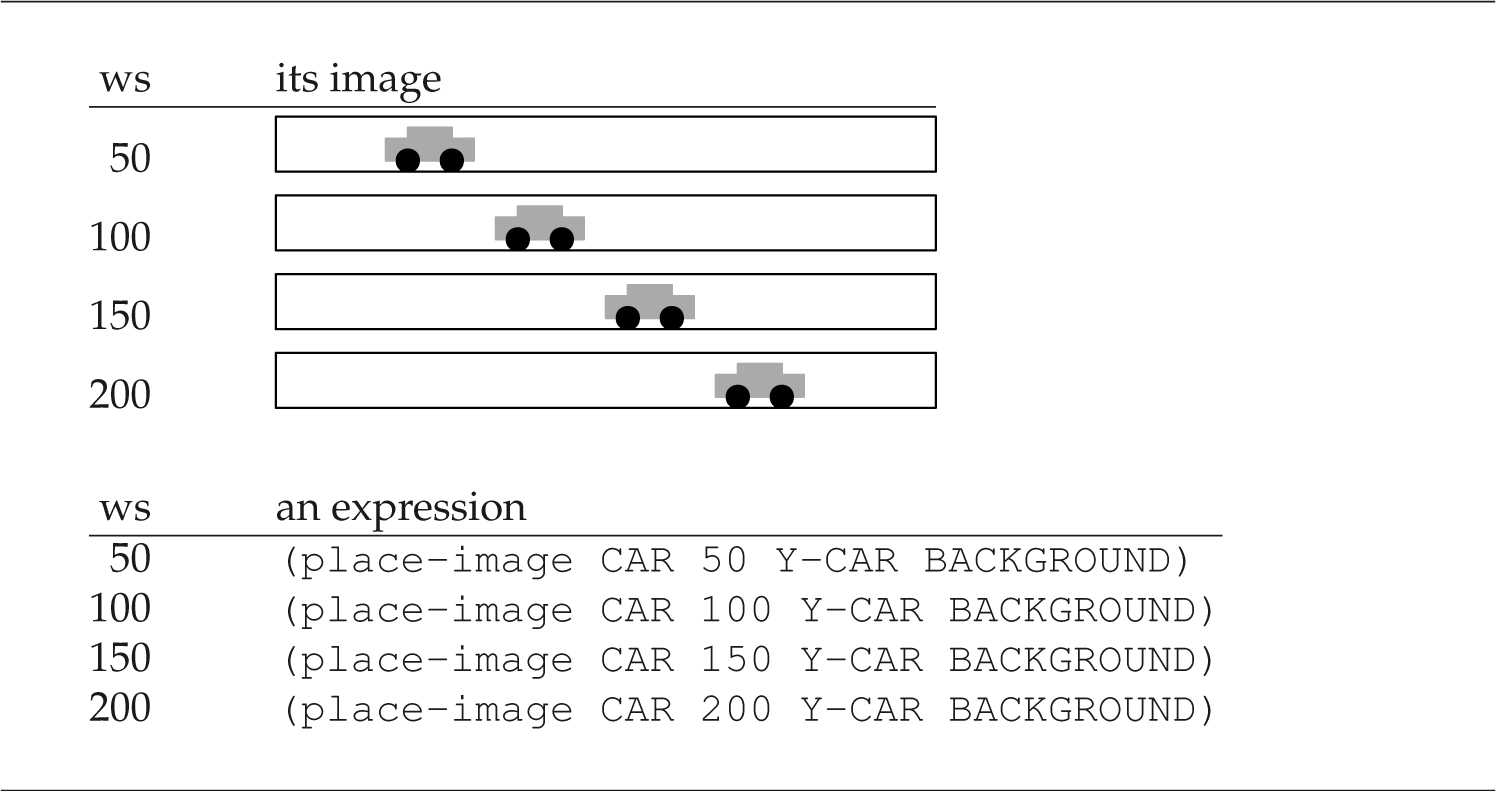
\includegraphics[width=0.85\textwidth]{images/00065.png}
  \caption{小车移动程序的视觉用例与代数表达式构造}
  \label{fig:ch03_car_examples}
\end{figure}

由此水到渠成地完成 \code{render} 的实现：
\begin{lstlisting}[language=BSL]
; WorldState -> Image
; 将小车按照当前状态 ws 绘制到背景画布 BACKGROUND 上
(define (render ws)
  (place-image CAR ws Y-CAR BACKGROUND))
\end{lstlisting}

\paragraph{第四步：编写 main 函数并点火运行}
将所有零件齐备后，主函数只需负责把初始状态和事件蓝图组装进 \code{big-bang} 中：
\begin{lstlisting}[language=BSL]
; WorldState -> WorldState
; launches the program from some initial state
(define (main ws)
   (big-bang ws
     [on-tick tock]
     [to-draw render]))
\end{lstlisting}

在交互区执行 \code{(main 13)}，你就能亲眼见证一辆小汽车从距左边缘 13 像素处平稳匀速驶向屏幕右侧！

\begin{exercise}{组装运行小车动画并添加树木背景}{41}
在完成练习~\ref{ex:39} 的基础上，定义 \code{BACKGROUND} 和 \code{Y-CAR} 常量，将上述所有函数组装成完整程序并在 DrRacket 中顺利运行。程序运转正常后，为背景增添一棵生动的绿树作为点缀。例如可以使用以下代码组合出一棵小树：
\begin{lstlisting}[language=BSL]
(define tree
  (underlay/xy (circle 10 "solid" "green")
               9 15
               (rectangle 2 20 "solid" "brown")))
\end{lstlisting}
此外，在 \code{big-bang} 中增加一个 \code{stop-when} 子句，使小汽车在完全开出右边界时自动优雅停止。
\end{exercise}

\begin{exercise}{修改状态诠释：小车右侧边缘坐标}{42}
修改上述数据定义的业务诠释：让世界状态 \code{WorldState} 表示小汽车\textbf{最右侧边缘}所在的横坐标位置。审视并重新调整你的渲染与判断逻辑。
\end{exercise}

\begin{exercise}{基于时间的动画状态设计与正弦运动}{43}
让我们用另一种极富洞见的视角重新审视上述问题：将世界状态定义为动画启动以来所经历的\textbf{绝对时钟滴答次数}：
\begin{lstlisting}[language=BSL]
; 一个 AnimationState 是一个 Number。
; 诠释：表示动画启动以来累计流逝的时钟滴答周期数
\end{lstlisting}
重新设计 \code{tock} 与 \code{render} 函数。进一步发挥数学魅力：利用三角函数 \code{sin} 设计一个小车沿着正弦波上下起伏前行的趣味动画世界！
\end{exercise}

\subsection{响应鼠标与超空间跃迁}

通过引入鼠标事件处理，我们能进一步体会“模型与视图彻底分离”所带来的无与伦比的架构弹性：
\begin{notebox}[案例拓展：超空间瞬间跃迁]
在原有小车匀速右移的基础上增加新特性：当用户在画布任意位置点击鼠标时，小汽车瞬间“跃迁”移动到该鼠标点击处的横坐标位置！
\end{notebox}

面对这一业务拓展，设计配方为我们提供了清晰的演进罗盘：
\begin{enumerate}
  \item 没有新增物理量，现有常量库无需变更；
  \item 动态演进的仍然只是小车的横坐标，现有数据定义 \code{WorldState} 依然完美适用；
  \item 唯一需要新增的，是处理鼠标点击的愿望条目：
\begin{lstlisting}[language=BSL]
; WorldState Number Number String -> WorldState
; 若鼠标事件 me 为 "button-down"，则将小车瞬间转移到 x-mouse 处
(define (hyper x-position-of-car x-mouse y-mouse me)
  x-position-of-car)
\end{lstlisting}
  \item 在主函数 \code{main} 的 \code{big-bang} 中直接追加一行 \code{[on-mouse hyper]} 即可：
\begin{lstlisting}[language=BSL]
(define (main ws)
  (big-bang ws
    [on-tick tock]
    [on-mouse hyper]
    [to-draw render]))
\end{lstlisting}
\end{enumerate}

接下来只需运用函数设计配方兑现 \code{hyper} 函数：
\begin{lstlisting}[language=BSL]
; WorldState Number Number String -> WorldState
; 鼠标点击处理函数
; 示例：
; 给定: 21 10 20 "enter",       期望: 21
; 给定: 42 10 20 "button-down", 期望: 10
; 给定: 42 10 20 "move",        期望: 42
(define (hyper x-position-of-car x-mouse y-mouse me)
  x-position-of-car)
\end{lstlisting}

\begin{exercise}{为鼠标事件编写 BSL 单元测试}{44}
将上述 \code{hyper} 函数的三个功能示例转化为正式的 \code{check-expect} 测试用例。在尚未写出实现之前运行，亲眼见证测试如期失败。
\end{exercise}

随后使用条件分支 \code{cond} 实现该函数：
\begin{lstlisting}[language=BSL, basicstyle=\scriptsize\ttfamily]
; WorldState Number Number String -> WorldState
; places the car at x-mouse
; if the given me is "button-down"
(define (hyper x-position-of-car x-mouse y-mouse me)
  (cond
    [(string=? "button-down" me) x-mouse]
    [else x-position-of-car]))
\end{lstlisting}
再次点击运行，测试全部通过！执行 \code{(main 1)}，尽情享受鼠标遥控小车瞬间跃迁的超快感！


% ==============================================================================
% 3.7 虚拟宠物世界
% ==============================================================================
\section{虚拟宠物世界}
\label{sec:3.7}

本节的综合项目练习将带领大家构建一个经典的电子虚拟宠物（Virtual Pet）游戏原型。我们的小猫会在画布上持续漫步前行；然而孤独漫步会让小猫逐渐感到失落不开心。正如真实宠物一样，你可以尝试抚摸小猫（提升一点快乐度），或者给它喂食小鱼干（让它超级开心满足）！

首先在代码中定义我们钟爱的小猫形象：
\begin{stepperbox}
\begin{Verbatim}[commandchars=\\\{\}, fontsize=\footnotesize]
(define cat1 \inlinesprite[2.2em]{images/sprites/cat1.png})
\end{Verbatim}
\end{stepperbox}

\begin{exercise}{虚拟宠物：循环移动的小猫}{45}
设计一个名为 \code{cat-prog} 的世界程序，让小猫以每个时钟周期 3 个像素的速度在屏幕上自左向右匀速漫步。该程序接收小猫的初始横坐标作为启动参数。当小猫从右侧边缘完全走出屏幕时，它能像环游世界一样，瞬间从最左侧边界重新出现并循环行进。

\textbf{提示：}查阅 DrRacket 帮助文档中的取模函数 \code{modulo}，思考它如何帮助实现无缝循环。
\end{exercise}

\begin{exercise}{双帧交替步态动画}{46}
为了让小猫的步伐更加生动逼真，我们准备了另一张迈出不同步伐的小猫图片：
\begin{stepperbox}
\begin{Verbatim}[commandchars=\\\{\}, fontsize=\footnotesize]
(define cat2 \inlinesprite[2.2em]{images/sprites/cat2.png})
\end{Verbatim}
\end{stepperbox}
修改练习~\ref{ex:45} 中的渲染函数：根据当前小猫横坐标数值是奇数还是偶数，交替选用两张不同姿态的小猫图片（查阅文档中的 \code{odd?} 谓词），从而呈现出生动连贯的漫步动画！
\end{exercise}

\begin{exercise}{虚拟宠物：设计快乐度计量表}{47}
设计一个独立的世界程序 \code{gauge-prog}，用来实时维护并显示宠物的“快乐度计量表”（happiness gauge）。程序接收初始最大快乐度数值。计量表以满分状态起步，随时间推移，每个时钟周期快乐度自然衰减 0.1；但无论如何衰减，快乐度最低不会跌破 0 分下限。

当玩家按下键盘上的【向下方向键】时，快乐度增加满分的 $1/5$；而每次按下【向上方向键】（代表喂食美味罐头），快乐度瞬间跳升满分的 $1/3$！

快乐度通过场景中央一个带有黑色外框的红色实心矩形进度条直观呈现：快乐度为 0 时红条消失；达到满分 100 时红条完整横跨画布。
\end{exercise}

\vspace{1em}
\begin{notebox}[更宏大的宠物世界愿景]
随着你在后续章节学到更多高阶复合数据结构，我们将向你揭示如何把练习~\ref{ex:45} 的行走小猫与练习~\ref{ex:47} 的心情仪表盘完美合体：漫步的小猫若长久无人理会就会日益沮丧；而当你抚摸它、喂饱它时，它会瞬间欢呼雀跃！这也是为什么在学完这前三章后，你必定会迫不及待地渴望探索更广阔程序设计世界的原因！
\end{notebox}

% ==============================================================================
% 第 4 章：区间、枚举与分类 (Chapter 4: Intervals, Enumerations, and Itemizations)
% ==============================================================================

\chapter{区间、枚举与分类}
\label{sec:ch04_intervals}

目前为止，你有四种将信息表示为数据的方式：数、字符串、图像与布尔值。对于许多简单问题，这四种基本类型已经足够；但在更多情况下，BSL（乃至任何编程语言）中这四种原始数据集合远远无法满足实际需求。真正的程序设计者需要更丰富的手段来将现实世界的信息表示为计算数据。

作为起步，优秀程序员必须学会对这些内置集合进行\term{约束与划分}。一种方法是从集合中明确\term{枚举}（enumerate）出一组离散的元素，并声明在此问题中只使用这些特定元素。显然，枚举仅适用于元素总数有限的情况。为了表示包含“无限”多个元素的集合，我们引入了\term{区间}（interval）——即满足某种特定数学属性的一组连续或离散的值。

\begin{notebox}[关于“无限”的说明]
这里的“无限”通常也可以指“规模大到对其逐一枚举在工程上完全不切实际”。
\end{notebox}

定义枚举与区间意味着我们需要对不同类型的数据进行区分。在代码中，区分不同的数据需要借助\term{条件函数}（conditional functions），即能够根据传入参数的具体取值选择不同计算路径的函数。在“多种计算方式”以及第 1.6 节中，我们已经见识过编写这类函数的示例。但当时的讨论并未涉及系统性的程序设计，而仅仅是在介绍 BSL 语言的新语法特性。

在本章中，我们将讨论适用于枚举与区间的通用设计方法。首先，我们重新审视 \code{cond} 条件表达式；接着依次探讨三种不同类型的数据描述方式：\term{枚举}（enumerations）、\term{区间}（intervals）和\term{分项数据 / 分类}（itemizations）。枚举会完整列出属于该集合的每一个数据元素；区间则指定一个连续或边界清晰的数据范围；而分类则将前两者融合在一起，在定义的某些分支中指定范围，在另一些分支中指定具体离散的数据。本章最后将归纳处理此类情况的通用设计配方，并探讨其在有限状态世界程序中的经典应用。

% ==============================================================================
\section{使用条件表达式编程}
\label{sec:4.1_programming_with_conditionals}
% ==============================================================================

回想我们在序幕中对条件表达式的简短介绍。由于 \code{cond} 是本书中涉及的最复杂表达式形式，让我们仔细观察其通用形式：

\begin{lstlisting}[language=BSL]
(cond
  [ConditionExpression_1 ResultExpression_1]
  [ConditionExpression_2 ResultExpression_2]
  ...
  [ConditionExpression_N ResultExpression_N])
\end{lstlisting}

\begin{notebox}[语法提示：方括号与圆括号]
方括号 \code{[...]} 的作用是让每个 \code{cond} 分支更加醒目。在 BSL 语法中，用普通圆括号 \code{(...)} 代替方括号也是完全合法的。
\end{notebox}

一个 \code{cond} 表达式以关键字 \code{(cond} 开头，并以匹配的 \code{)} 结尾。紧随关键字之后，程序员可以书写任意多个 \code{cond} 行（行数视需求而定）；每一行包含两个表达式，由左右方括号 \code{[} 与 \code{]} 包裹。

一个 \code{cond} 行在专业术语中在术语上被称为一个 \code{cond} \term{条件分支}（或\term{条件子句}，cond clause）。

下面是一个使用条件表达式的函数定义：

\begin{lstlisting}[language=BSL]
(define (next traffic-light-state)
  (cond
    [(string=? "red" traffic-light-state) "green"]
    [(string=? "green" traffic-light-state) "yellow"]
    [(string=? "yellow" traffic-light-state) "red"]))
\end{lstlisting}

就像序幕中的数学分段函数一样，这个例子展示了使用 \code{cond} 表达式的便利之处。在许多问题场景中，函数必须区分若干种互斥的情况。借助 \code{cond} 表达式，你可以为每种可能性分配单独的一行，从而直观地对应于问题描述中的各个分支。

\begin{notebox}[编程实践备忘：cond 与 if 的选择]
请对比 \code{cond} 表达式与第 1.6 节中的 \code{if} 表达式。\code{if} 表达式擅长将“一种情况与其余所有情况”区分开来（二选一）。因此，当面对多重情况时，嵌套的 \code{if} 会变得极其冗长且难以阅读。我们达成一个共识：只要分支直接源于数据定义中的多种情况，就一律使用 \code{cond}；只有在表达单纯的“非此即彼”二选一时，才使用 \code{if}。
\end{notebox}

当 \code{cond} 表达式中的条件判断变得繁琐时，你有时希望表达“在其余所有情况下”的兜底语义。为此，BSL 允许在 \code{cond} 表达式的\textbf{最后一行}使用关键字 \code{else}：

\begin{lstlisting}[language=BSL]
(cond
  [ConditionExpression_1 ResultExpression_1]
  [ConditionExpression_2 ResultExpression_2]
  ...
  [else DefaultResultExpression])
\end{lstlisting}

如果你误在其他位置使用了 \code{else}，DrRacket 会立即报错：

\begin{replbox}
> (cond
    [(> x 0) 10]
    [else 20]
    [(< x 10) 30])
cond: found an else clause that isn't the last clause in its cond expression
\end{replbox}

也就是说，BSL 严格拒绝在语法上无意义或歧义的结构。

假设我们要设计一个在游戏结束时计算奖励等级的函数。下面是该函数的签名与说明：

\begin{lstlisting}[language=BSL]
; PositiveNumber 代表非负数（即大于或等于 0 的数）
; PositiveNumber -> String
; 根据给定的得分 s 计算对应的奖励等级
\end{lstlisting}
\footnote{严格在数学上，大于或等于 0 的数称为“非负数”（Non-negative Number），严格大于 0 的数才称为“正数”（Positive Number）。原书在此处为了降低初学者门槛，宽松地使用了 \code{PositiveNumber} 作为类型名来指代 $[0, \infty)$ 区间。本书在代码中沿用原书标识符以保持与练习和测试用例一致，正文表述中统一明确其非负数含义。}

下面给出两种对比实现：

\begin{figure}[htbp]
  \centering
  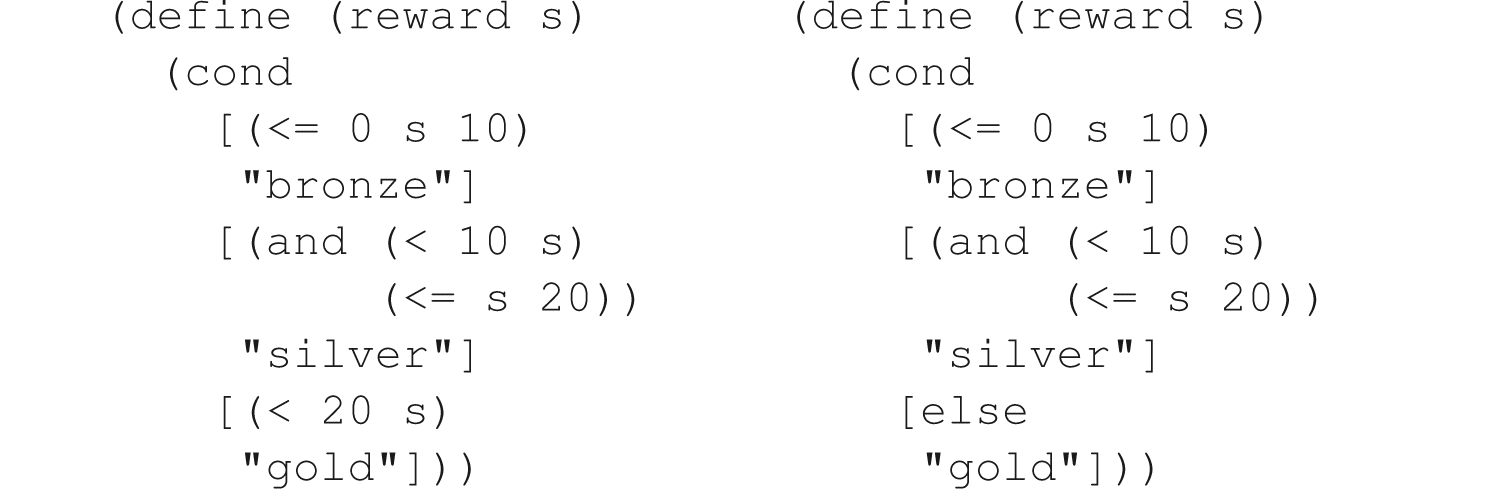
\includegraphics[width=0.85\textwidth]{images/00071.png}
  \caption{显式全条件（左）与使用 else 分支（右）的对比}
  \label{fig:reward_compare}
\end{figure}

左侧变体使用了包含三个完整布尔条件的 \code{cond}；而右侧则在末尾使用了 \code{else} 分支。为了推导左侧第三个条件 \code{(< 20 s)}，你必须在头脑中计算推断出：
\begin{itemize}
  \item $s$ 是一个 \code{PositiveNumber}（即非负数）；
  \item \code{(<= 0 s 10)} 的求值结果为 \code{\#false}；
  \item \code{(and (< 10 s) (<= s 20))} 的求值结果同样为 \code{\#false}。
\end{itemize}

尽管在这个简单例子中心算并不复杂，但当业务规则变得交错时，手动推导互补条件极易出错并埋下隐患。因此，当你明确需要对前述所有条件取反（即逻辑上的\term{补集}，complement）时，使用右侧带有 \code{else} 的写法更为稳妥清晰。

\begin{exercise}{单步调试奖励函数}{48}
将 \code{reward} 的函数定义以及测试调用 \code{(reward 18)} 键入 DrRacket 的定义区，并点击“单步求值器”（Stepper），观察 DrRacket 是如何一步步对函数应用进行求值的。
\end{exercise}

\begin{exercise}{嵌套条件表达式}{49}
\code{cond} 本身就是一个表达式，因此它完全可以嵌套在另一个表达式内部。例如：
\begin{lstlisting}[language=BSL]
(- 200 (cond [(> y 200) 0] [else y]))
\end{lstlisting}

请参考图~\ref{fig:ch04_rocket_recall} 中的 \code{create-rocket-scene.v5} 函数，重构该函数并使用嵌套的 \code{cond} 表达式，使得新函数体中仅出现一次 \code{place-image} 调用。

\begin{center}
  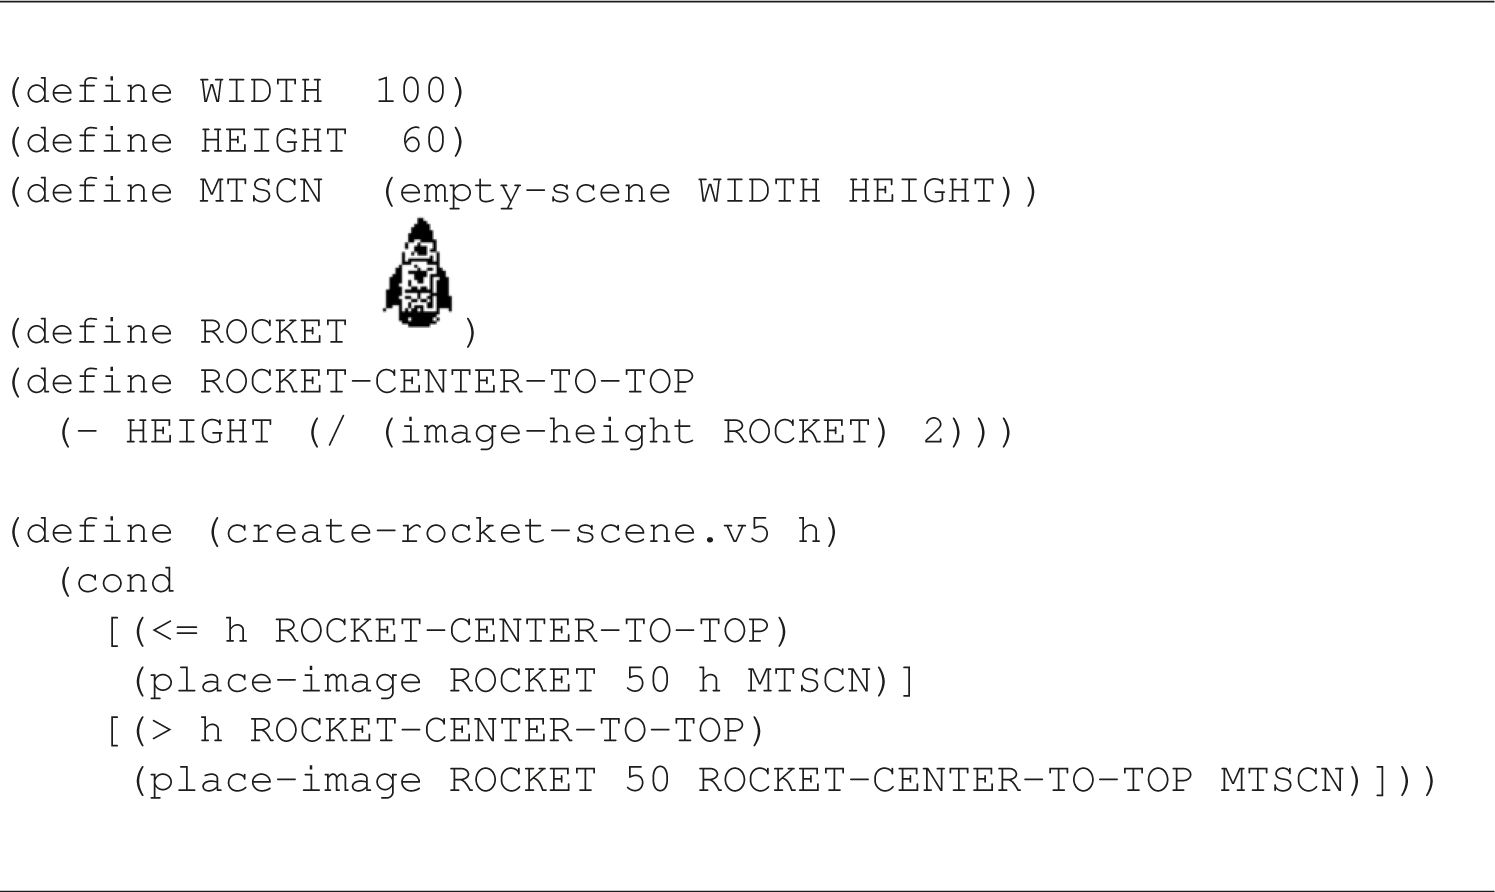
\includegraphics[width=0.75\textwidth]{images/00072.jpeg}
  \captionof{figure}{火箭发射场景生成函数}\label{fig:ch04_rocket_recall}
\end{center}
\end{exercise}

% ==============================================================================
\section{条件计算过程}
\label{sec:4.2_computing_conditionally}
% ==============================================================================

理解条件表达式的核心在于掌握其严格的求值规则。其计算归约（reduction）过程遵循以下规则：

\begin{notebox}[cond 表达式的求值规则]
对于形如 \code{(cond [C\_1 R\_1] [C\_2 R\_2] ...)} 的表达式：
\begin{enumerate}
  \item DrRacket 从上到下依次对条件表达式 $C_i$ 求值。
  \item 若 $C_1$ 求值结果为 \code{\#true}，则整个 \code{cond} 表达式立刻被替换为其对应的结果表达式 $R_1$。
  \item 若 $C_1$ 求值结果为 \code{\#false}，则该条件分支被完全丢弃，计算继续对剩下的分支进行。
  \item 若 $C_1$ 的求值结果既非 \code{\#true} 亦非 \code{\#false}，BSL 报错：\code{cond: question result is not true or false}。
  \item 若遭遇 \code{[else R]}，它无条件等价于 \code{\#true}，整个表达式直接被替换为 $R$。
  \item 若所有条件均为 \code{\#false} 且没有 \code{else} 分支，BSL 报错：\code{cond: all question results were false}。
\end{enumerate}
\end{notebox}

让我们以 \code{(reward 3)} 的计算为例进行单步追踪：
\begin{lstlisting}[language=BSL]
  (reward 3)
== (cond
     [(<= 0 3 10) "bronze"]
     [(and (< 10 3) (<= 3 20)) "silver"]
     [else "gold"])
== (cond
     [#true "bronze"]
     [(and (< 10 3) (<= 3 20)) "silver"]
     [else "gold"])
== "bronze"
\end{lstlisting}

再看当输入为 21 时的情况：
\begin{lstlisting}[language=BSL]
  (reward 21)
== (cond
     [(<= 0 21 10) "bronze"]
     [(and (< 10 21) (<= 21 20)) "silver"]
     [else "gold"])
== (cond
     [#false "bronze"]
     [(and (< 10 21) (<= 21 20)) "silver"]
     [else "gold"])
== (cond
     [(and (< 10 21) (<= 21 20)) "silver"]
     [else "gold"])
== (cond
     [(and #true (<= 21 20)) "silver"]
     [else "gold"])
== (cond
     [(and #true #false) "silver"]
     [else "gold"])
== (cond
     [#false "silver"]
     [else "gold"])
== (cond
     [else "gold"])
== "gold"
\end{lstlisting}

\begin{exercise}{测试覆盖度}{50}
如果你将本章第一节的 \code{next} 函数复制到 DrRacket 定义区并点击“Run”，DrRacket 会高亮显示三行 \code{cond} 中的两行（颜色通常为黑色背景加亮）。这种高亮表示你的测试用例未能覆盖所有的条件分支。请补充足够的测试用例，使测试覆盖所有情况。
\end{exercise}

\begin{exercise}{模拟红绿灯世界程序}{51}
设计一个使用 \code{big-bang} 的世界程序，在指定的时间跨度内模拟交通信号灯的状态变迁。程序将信号灯的状态渲染为一个填充了对应颜色的实心圆，并且在每个时钟滴答（clock tick）发生时改变颜色。哪种颜色是最合适的初始状态？不妨咨询一下工程专业的朋友。
\end{exercise}

% ==============================================================================
\section{枚举}
\label{sec:4.3_enumerations}
% ==============================================================================

在程序设计中，当现实中的状态仅存在有限个离散可能时，我们使用\term{枚举}（Enumeration）来定义数据。

\begin{lstlisting}[language=BSL]
; 一个 TrafficLight 是以下三者之一：
; -- "red"
; -- "green"
; -- "yellow"
; 解释：交通信号灯的三种法定显示颜色
\end{lstlisting}

数据定义的核心目的在于：向读者明确指出该集合包含哪些值，以及这些值在现实世界中对应什么物理含义。在枚举中，我们逐一列出属于该集合的所有合法值。

除了自定义枚举，BSL 还提供了若干内置的大型枚举，最典型的便是按键事件 \code{KeyEvent} 和鼠标事件 \code{MouseEvent}。一个 \code{KeyEvent} 本质上是一个包含上百个合法字符串的枚举（如 \code{"a"}, \code{"b"}, \code{"left"}, \code{"right"}, \code{"\ "} 等）。

\begin{figure}[htbp]
  \centering
  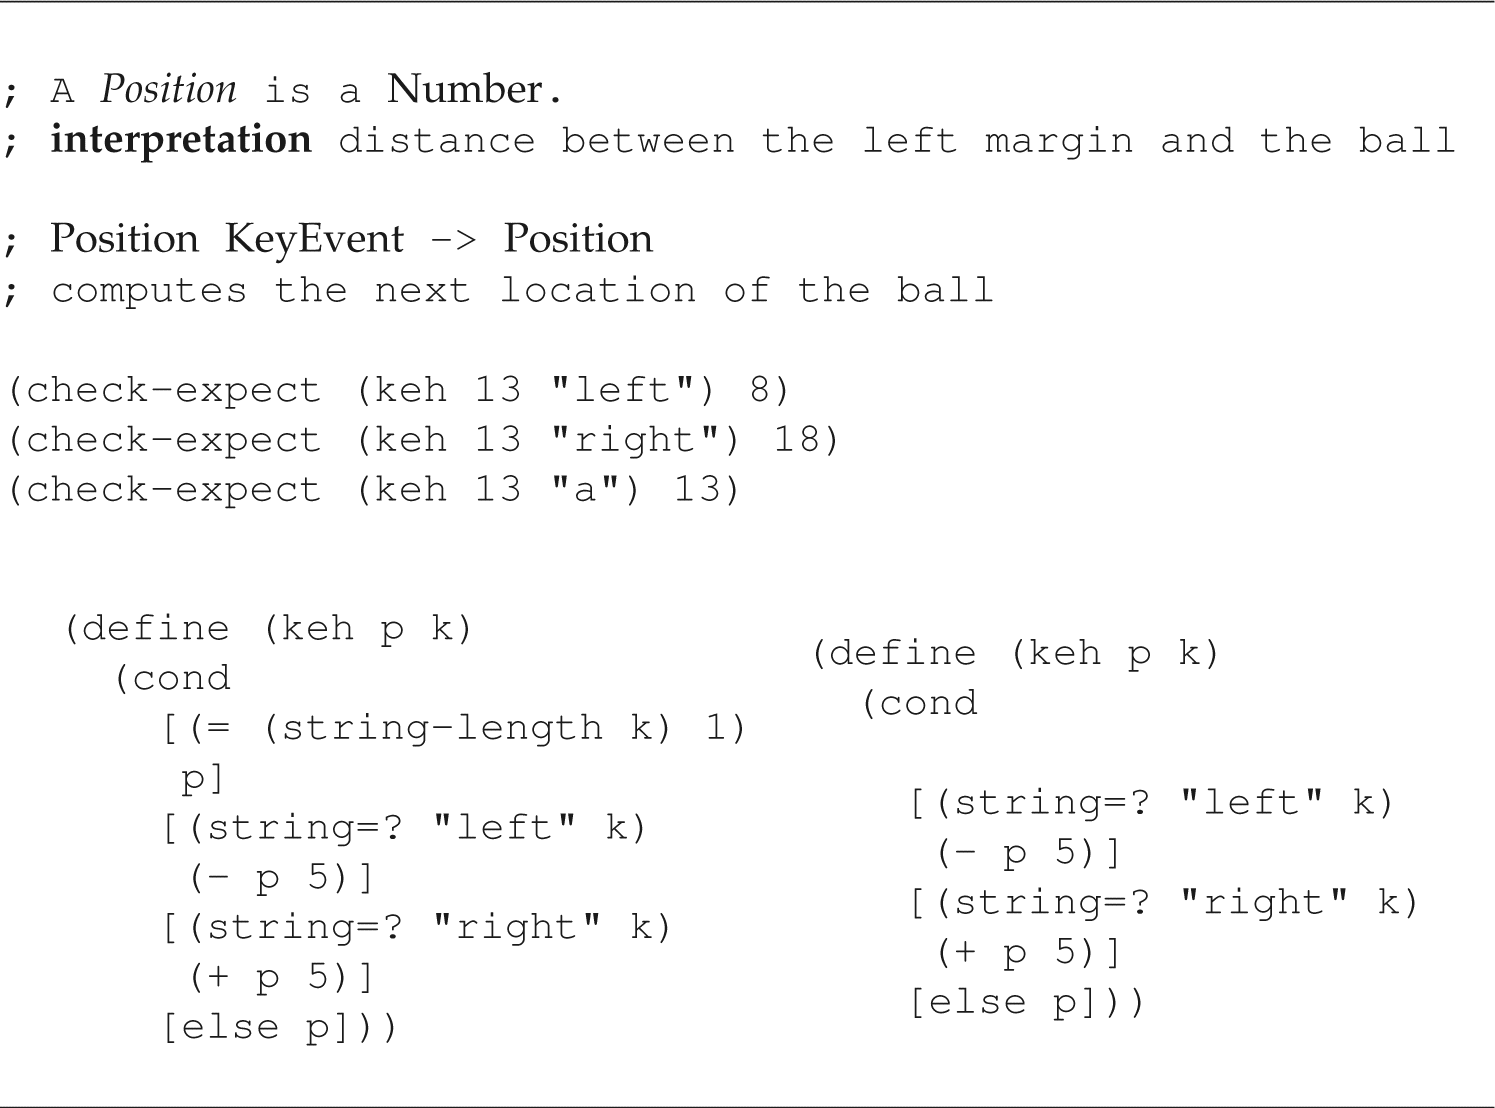
\includegraphics[width=0.9\textwidth]{images/00073.png}
  \caption{条件函数与特殊枚举处理的两种方式}
  \label{fig:deal_with_keys_compare}
\end{figure}

图~\ref{fig:deal_with_keys_compare} 展示了处理枚举的两种思路。左侧遵循“数据定义的每一项对应 \code{cond} 的一行”的标准规范；右侧则针对特殊场景进行了精简重组：将我们关心的两颗方向键单独处理，其他所有未关心的按键统统归入 \code{else}。这种代码重构通常应当在按照设计配方完成基础设计之后再审慎进行。

% ==============================================================================
\section{区间}
\label{sec:4.4_intervals}
% ==============================================================================

当可能的数据量非常庞大或连续时，枚举就无能为力了。此时我们使用\term{区间}（Interval）来圈定数据范围。

数学上，我们使用开区间与闭区间的符号体系：
\begin{itemize}
  \item $[a, b]$ 表示包含两端点的闭区间：$\{x \in \mathbb{R} \mid a \le x \le b\}$；
  \item $(a, b)$ 表示不包含两端点的开区间：$\{x \in \mathbb{R} \mid a < x < b\}$；
  \item $[a, b)$ 和 $(a, b]$ 分别表示半开半闭区间；
  \item $[a, \infty)$ 表示无上界的右向无穷区间：$\{x \in \mathbb{R} \mid x \ge a\}$。
\end{itemize}

在数据定义中，我们可以清晰地书写区间：
\begin{lstlisting}[language=BSL]
; A PositiveNumber is a Number greater than/equal to 0.
; 一个非负数（原书类型名作 PositiveNumber）是大于或等于 0 的数：[0, \infty)
\end{lstlisting}

\begin{figure}[htbp]
  \centering
  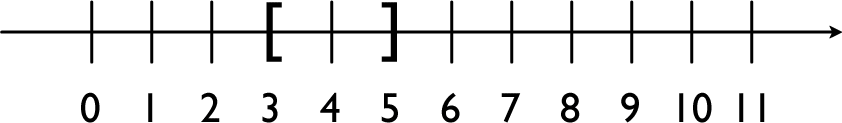
\includegraphics[width=0.6\textwidth]{images/00075.png}\\[1ex]
  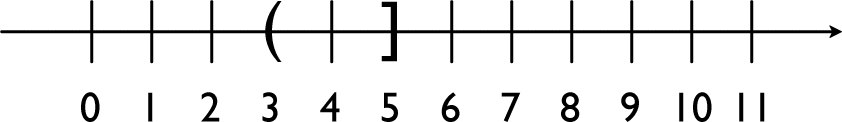
\includegraphics[width=0.6\textwidth]{images/00076.png}\\[1ex]
  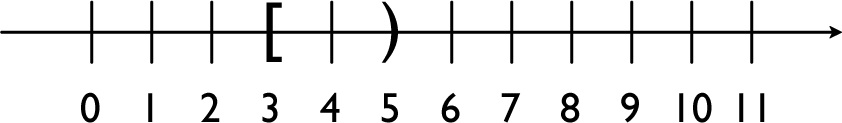
\includegraphics[width=0.6\textwidth]{images/00077.png}\\[1ex]
  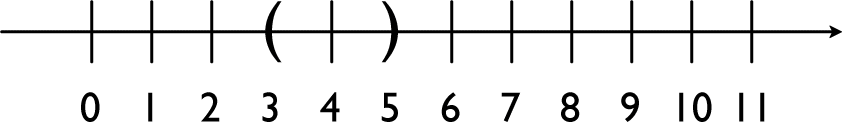
\includegraphics[width=0.6\textwidth]{images/00078.png}\\[1ex]
  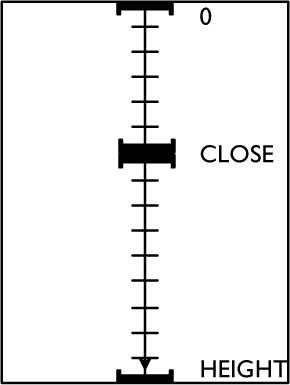
\includegraphics[width=0.6\textwidth]{images/00079.png}
  \caption{各类型区间的数轴可视化}
  \label{fig:number_lines}
\end{figure}

数轴可视化（图~\ref{fig:number_lines}）在两方面极大地指导了函数设计：
\begin{enumerate}
  \item 它直观指引了\textbf{测试用例的选取}：我们不仅需要在区间的“内部”挑选典型点，还必须精确选取区间的“端点”（边界条件），因为边界是最容易出现 $\le$ 与 $<$ 混淆的地方。
  \item 它明确了\textbf{条件判断的公式}：例如判定一个数 $x$ 是否位于 $[3, 5]$ 内，条件表达式应写作 \code{(<= 3 x 5)}。
\end{enumerate}

\begin{exercise}{区间整数判定}{52}
观察上述四幅数轴图，分别指出各个区间内包含哪些整数？
\end{exercise}

\subsection{案例研究：UFO 降落程序}

让我们考虑一个 UFO 从天空中降落的交互式程序。
如图~\ref{fig:ufo_descending} 所示，我们首先确立基础常数与数据定义：

\begin{figure}[htbp]
  \centering
  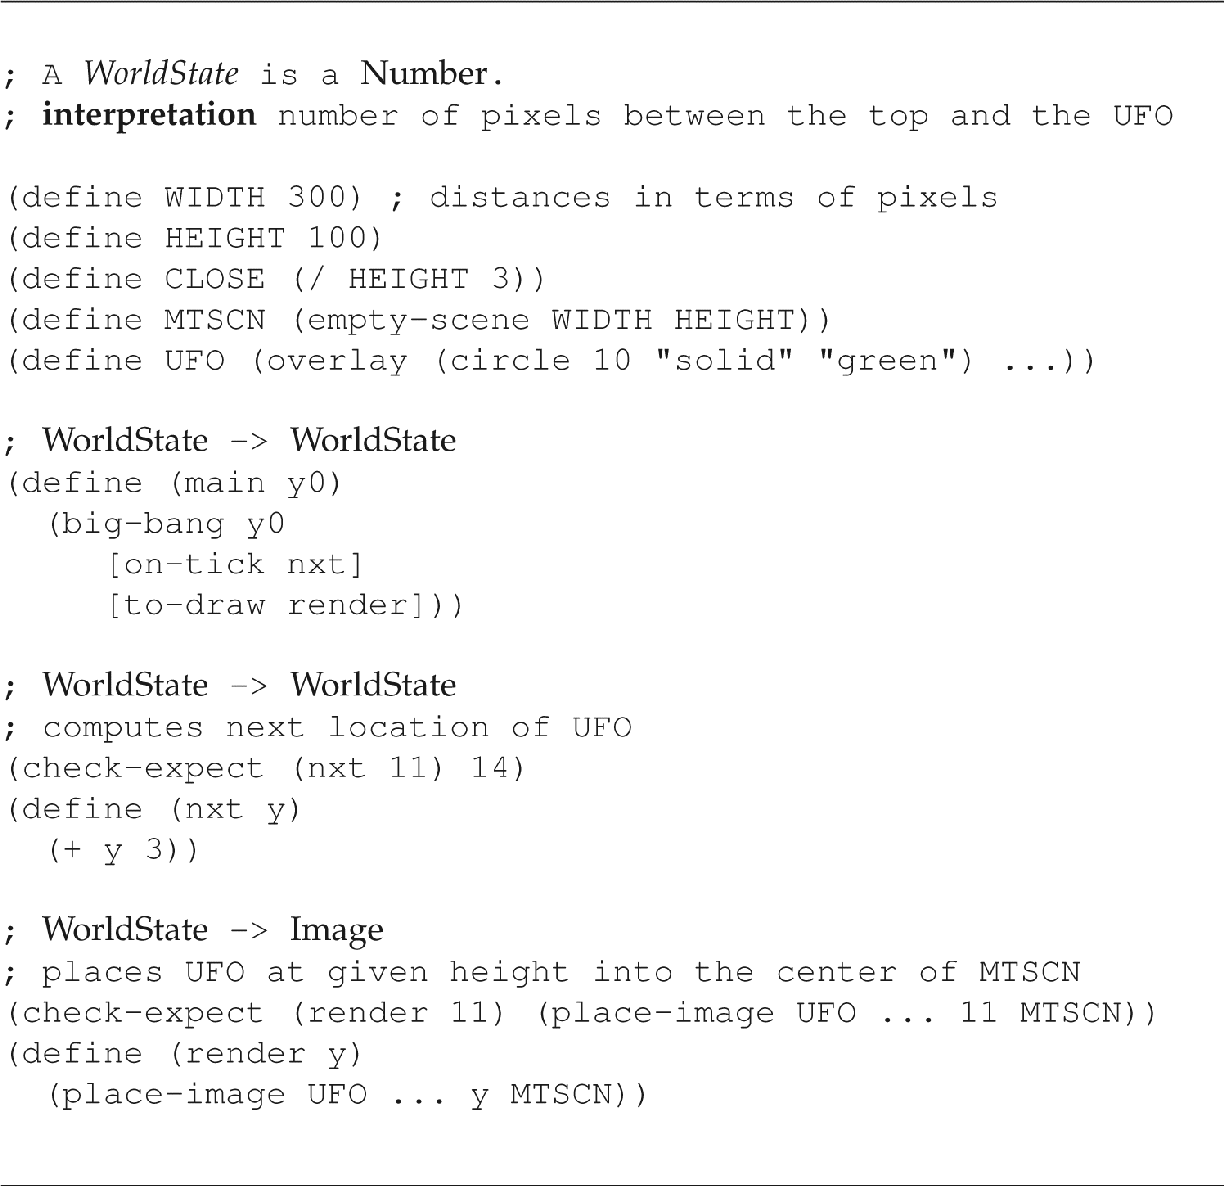
\includegraphics[width=0.85\textwidth]{images/00074.png}
  \caption{UFO 降落的世界程序骨架}
  \label{fig:ufo_descending}
\end{figure}

\begin{lstlisting}[language=BSL]
(define WIDTH 300)
(define HEIGHT 100)
(define CLOSE (/ HEIGHT 3))
(define MTSCN (empty-scene WIDTH HEIGHT))
(define UFO (overlay (circle 10 "solid" "green")
                     (rectangle 40 4 "solid" "green")))

; 一个 WorldState 是一个非负数 Number
; 解释：UFO 中心距离顶部的像素高度
\end{lstlisting}

现在我们希望为画面添加状态文本行：
\begin{itemize}
  \item 当 $0 \le y \le \text{CLOSE}$ 时，处于“降落中”（descending，显示为绿色）；
  \item 当 $\text{CLOSE} < y \le \text{HEIGHT}$ 时，处于“接近地面”（closing in，显示为橙色）；
  \item 当 $y > \text{HEIGHT}$ 时，处于“已着陆”（landed，显示为红色）。
\end{itemize}

\begin{figure}[htbp]
  \centering
  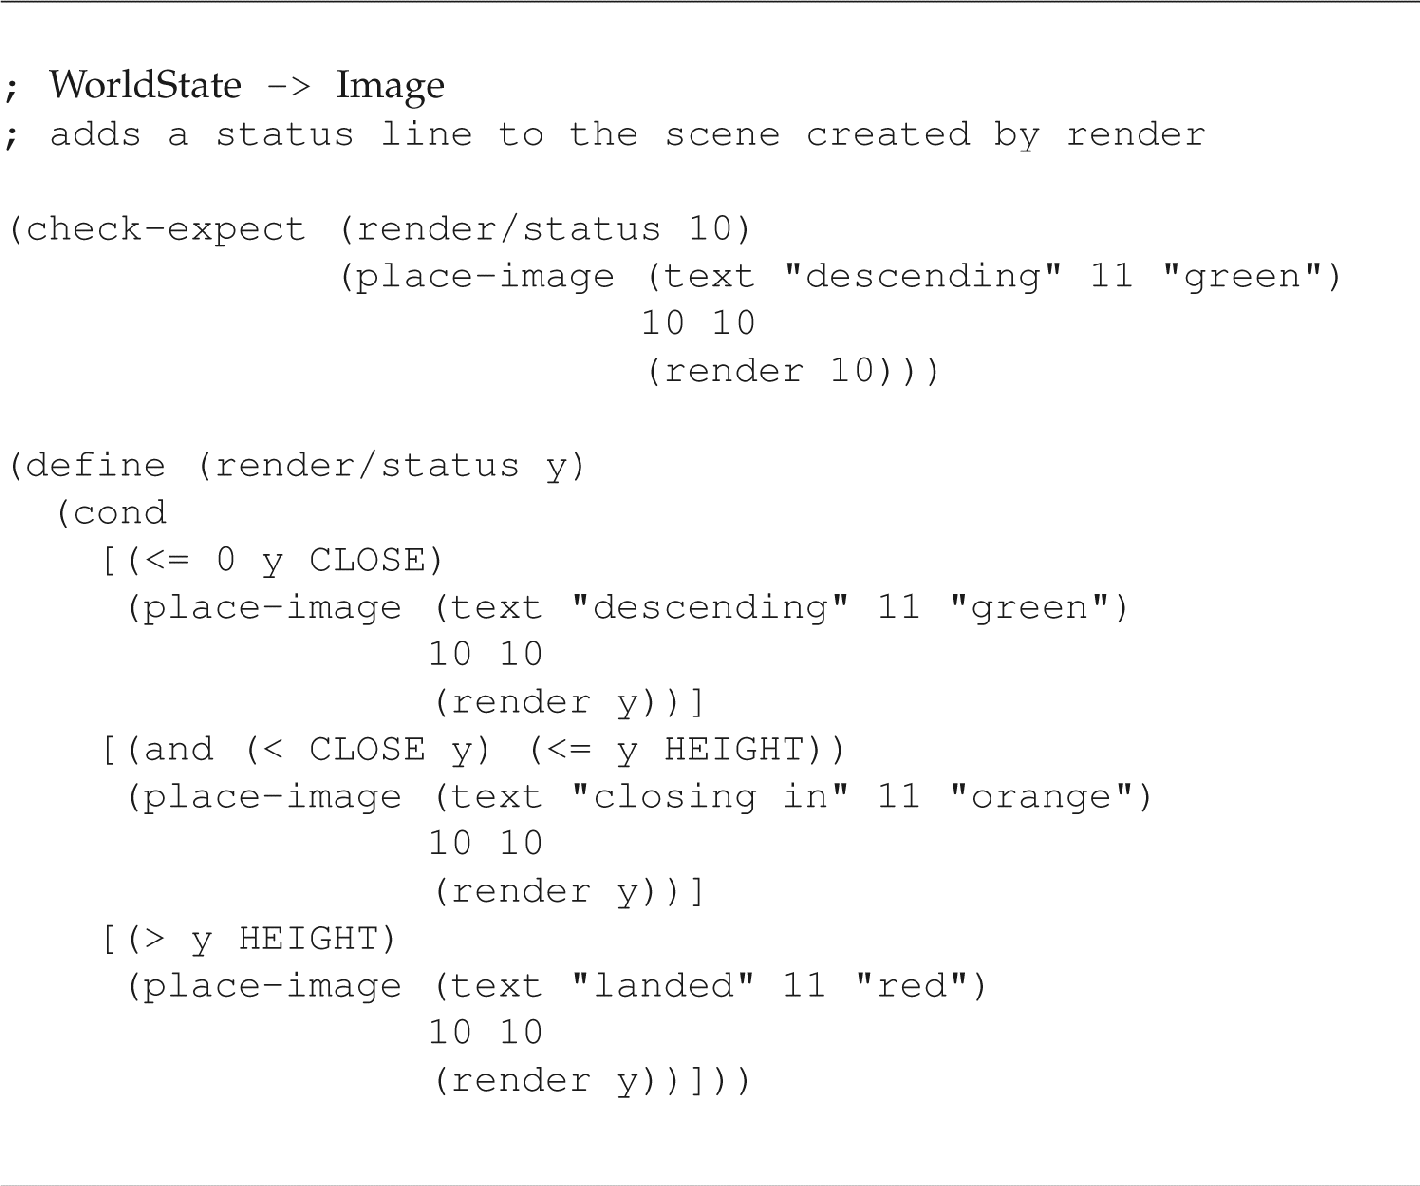
\includegraphics[width=0.85\textwidth]{images/00082.png}
  \caption{带有状态提示栏的渲染函数 render/status}
  \label{fig:render_status_orig}
\end{figure}

图~\ref{fig:render_status_orig} 给出了初版 \code{render/status} 的完整定义。观察该定义，三个分支中均出现了重复的渲染框架。通过将 \code{cond} 表达式嵌套在 \code{text} 的参数中，我们可以将其优雅地重构为图~\ref{fig:render_status_revised} 所示的形式。

\begin{figure}[htbp]
  \centering
  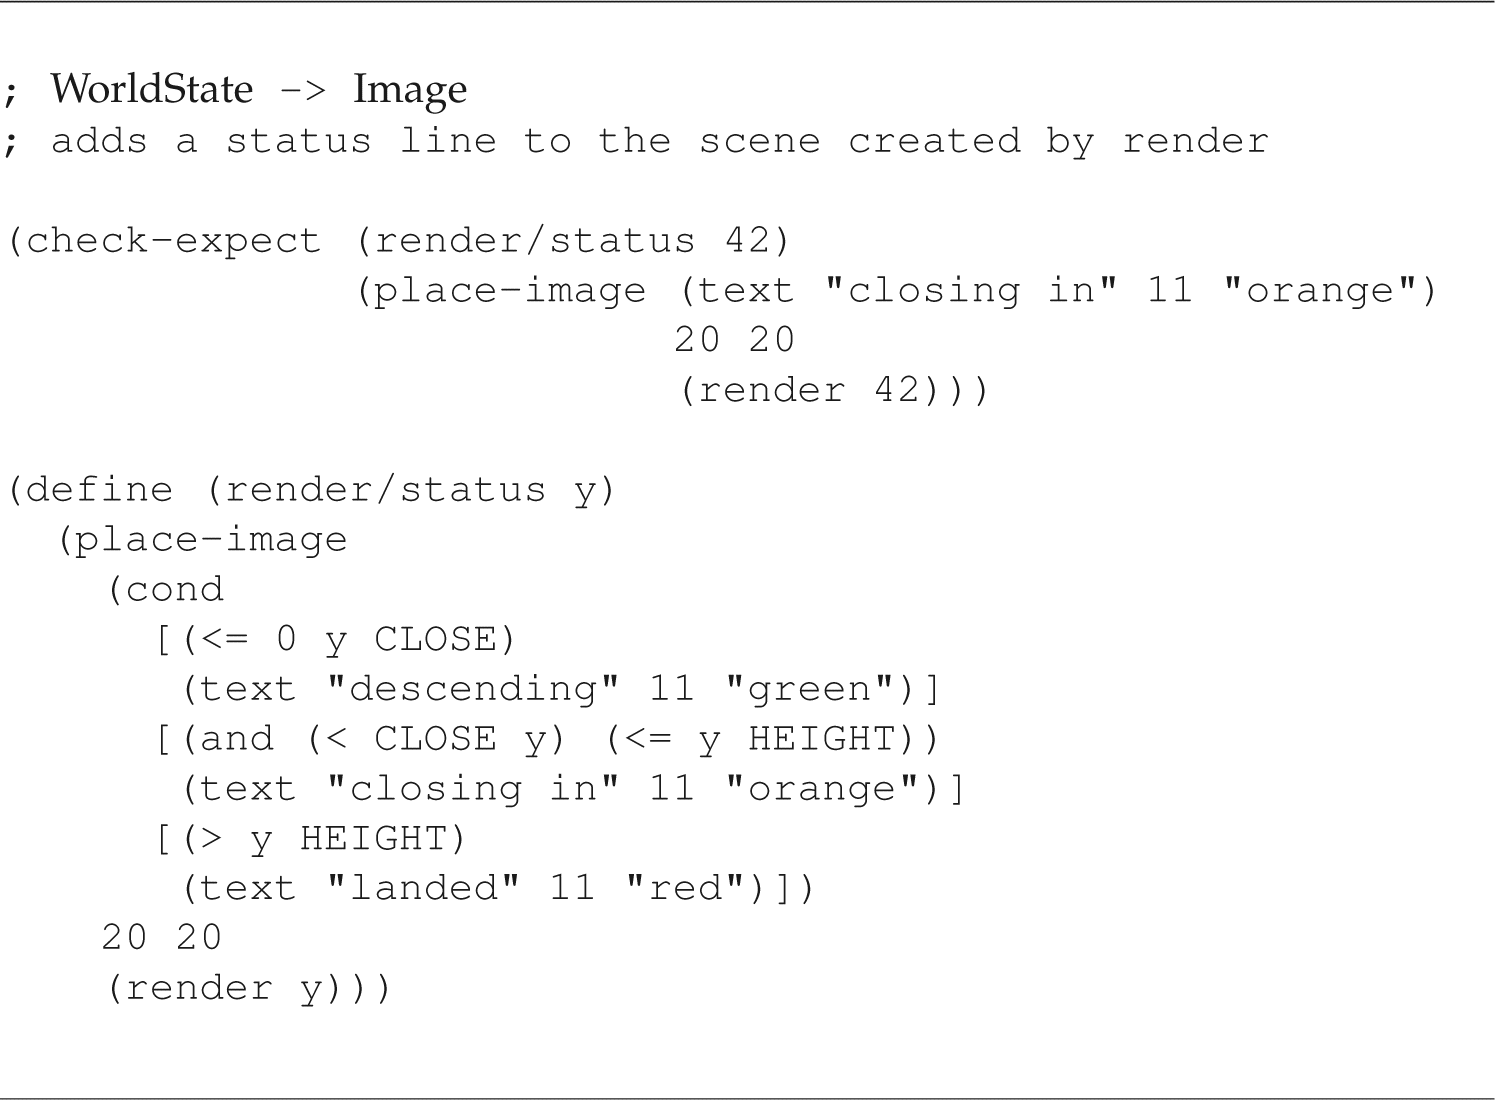
\includegraphics[width=0.85\textwidth]{images/00084.png}
  \caption{重构后的 render/status 函数}
  \label{fig:render_status_revised}
\end{figure}

% ==============================================================================
\section{分类 / 分项数据}
\label{sec:4.5_itemizations}
% ==============================================================================

在更复杂的世界中，一个状态量可能既包含区间，又包含若干特殊的离散标记。这种将不同性质的数据集合进行并集组合的数据描述称为\term{分类}或\term{分项数据}（Itemization）。

考虑一个火箭发射倒计时的世界程序。火箭在发射前处于静止状态，接着进行倒数（$-3, -2, -1$），最后点火升空并不断增加高度。我们可以将世界状态定义为：

\begin{lstlisting}[language=BSL]
; 一个 LRCD (火箭发射与倒计时状态) 是以下三者之一：
; -- "resting"
; -- 处于 [-3, -1] 之间的整数
; -- 一个非负数 NonNegativeNumber
; 解释：
; "resting" 表示火箭静止在发射架上；
; 负数代表发射前的倒计时秒数；
; 非负数代表火箭升空后距离地面的高度。
\end{lstlisting}

\begin{figure}[htbp]
  \centering
  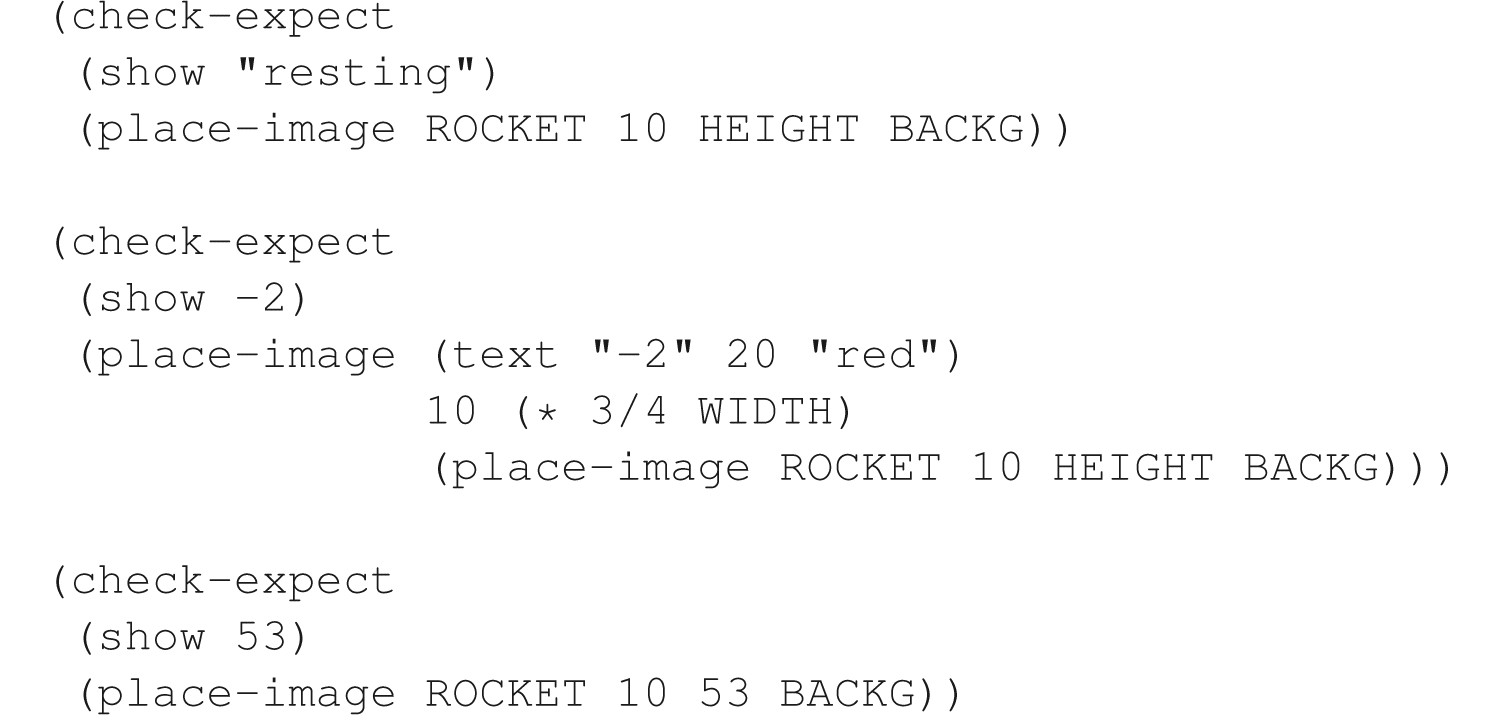
\includegraphics[width=0.7\textwidth]{images/00085.png}
  \caption{LRCD 状态的视觉示意图}
  \label{fig:lrcd_scenes}
\end{figure}

\begin{figure}[htbp]
  \centering
  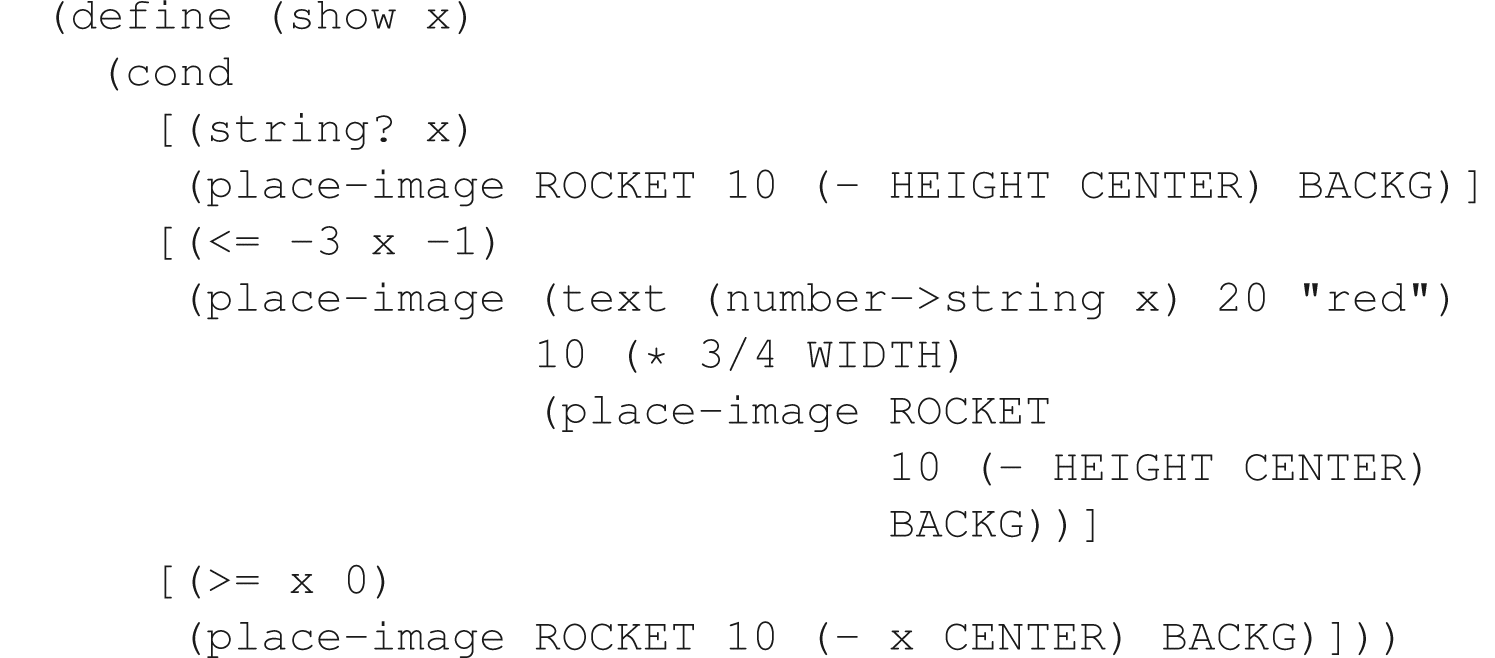
\includegraphics[width=0.8\textwidth]{images/00086.png}
  \caption{针对分类数据 LRCD 的函数模板骨架}
  \label{fig:lrcd_template}
\end{figure}

在图~\ref{fig:lrcd_template} 中，每一个分支条件严格对应数据定义的一个子类别。特别需要注意：在判定 \code{"resting"} 时，不能直接使用 \code{(string=? "resting" x)}，因为当参数 $x$ 为数时，\code{string=?} 会引发类型错误！必须使用更加安全的谓词或组合判断。

图~\ref{fig:ch04_rocket_full} 给出了该程序的各个关键事件处理函数的完整设计。

\begin{figure}[htbp]
  \centering
  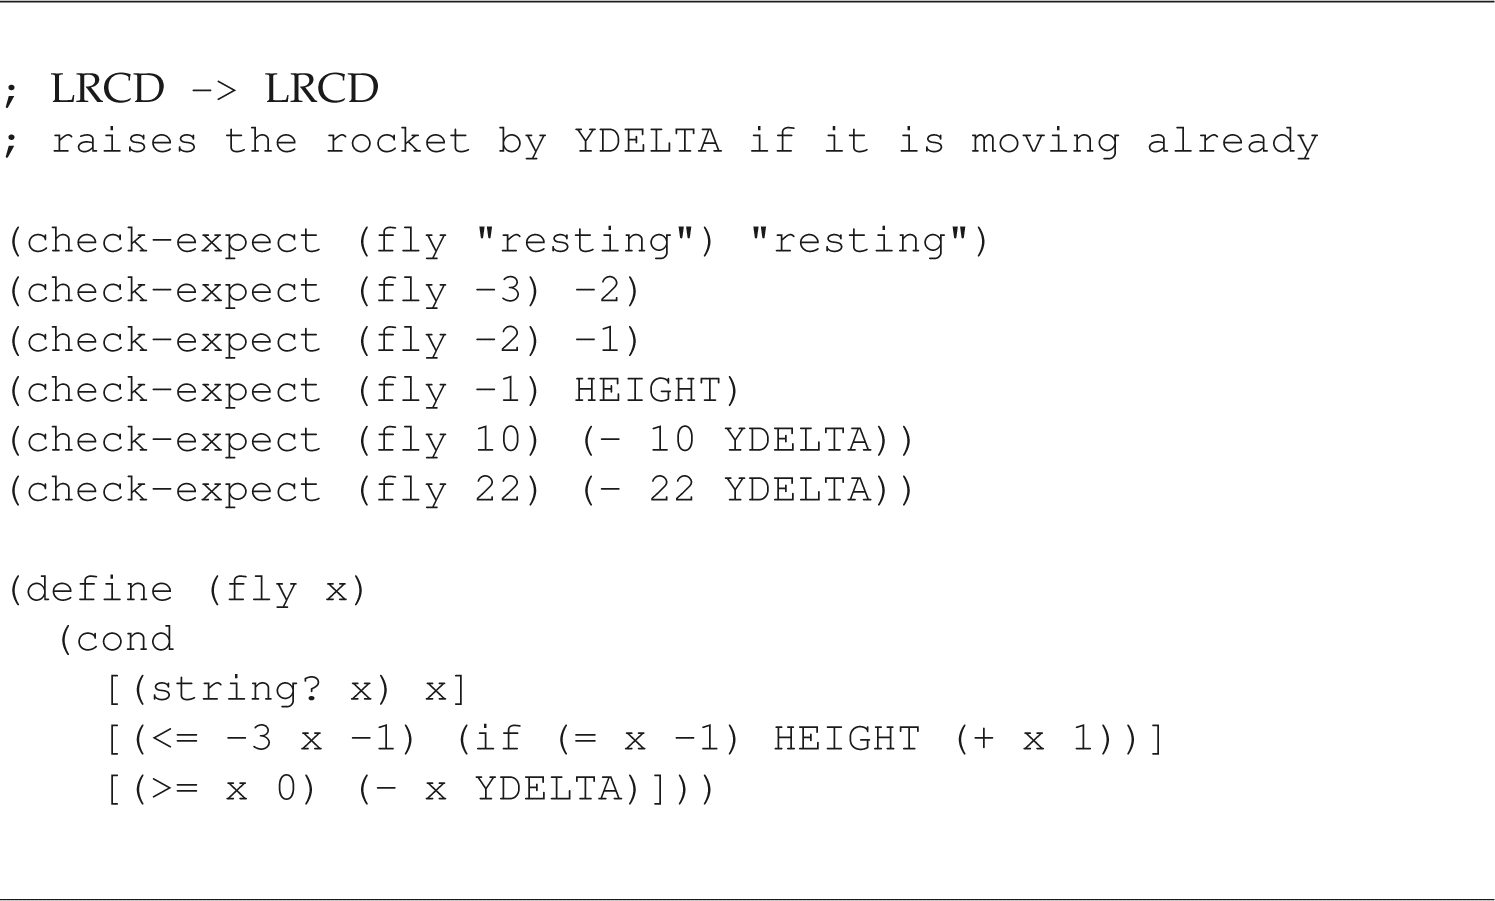
\includegraphics[width=0.9\textwidth]{images/00087.png}
  \caption{火箭发射倒计时程序的完整代码}
  \label{fig:ch04_rocket_full}
\end{figure}

\begin{exercise}{信息与数据的互转}{53}
世界程序的设计配方要求程序员能够在“现实信息”与“程序数据”之间自如转换。请根据 LRCD 的定义，绘制若干代表不同世界场景的草图，并写出对应的数据表示；反过来，选取至少包含 $0$ 和 \code{HEIGHT} 在内的几个数据样例，绘制其对应的场景图像。
\end{exercise}

\begin{exercise}{精确的条件谓词}{54}
为什么在 \code{show} 函数中将第一个条件写为 \code{(string=? "resting" x)} 是错误的？请写出一个完全严谨的条件表达式，使得它在且仅在 $x$ 属于 LRCD 的第一个子类时求值为 \code{\#true}。
\end{exercise}

\begin{exercise}{提取公共辅助函数}{55}
重新审视 \code{show} 函数。它包含了三处大致形如 \code{(place-image ROCKET 10 ... BACKG)} 的绘制逻辑。请设计一个辅助函数简化这些重复代码。
\end{exercise}

\begin{exercise}{完整的发射主程序}{56}
定义 \code{main2} 函数，使你能够按下空格键启动倒计时并亲眼目睹火箭升空。查阅 \code{on-tick} 子句的文档，了解一个滴答的默认时长以及如何自定义时钟频率。
\end{exercise}

\begin{exercise}{高度的另一种几何诠释}{57}
在物理学和计算机图形学中，“高度”可以有两种理解：距离地面的高度（自底向上）或在画布中的坐标（自顶向下）。重做本节的练习，改用另一种诠释方式，并对比两套方案的异同。
\end{exercise}

% ==============================================================================
\section{针对分类数据的设计}
\label{sec:4.6_designing_with_itemizations}
% ==============================================================================

现在我们提炼出针对\term{分类数据}（Itemization）的通用设计配方：

\begin{recipebox}{设计针对分类数据的函数}
\begin{enumerate}
  \item \textbf{数据定义}：明确列出所有互斥的子类（分支）。每个子类可以是具体的值、一个枚举、一个区间或甚至另一个类型。
  \item \textbf{签名、目的说明与函数头}：根据数据定义确定输入输出类型，简述函数计算逻辑，列出形参名。
  \item \textbf{功能示例}：\textbf{为每个子类至少设计一个典型示例}！对于包含区间的子类，必须在区间内部选取测试点，并在区间所有端点（边界）处各选取一个测试点。
  \item \textbf{函数模板}：
    \begin{itemize}
      \item 根据数据定义中子类的个数，写出包含同样数量分支的 \code{cond} 表达式；
      \item 为每个分支构思严密且互斥的条件判定表达式（Condition Expressions）；
      \item 留出结果表达式占位符 \code{...}。
    \end{itemize}
  \item \textbf{函数体实现}：针对每一个分支，结合该分支所承诺的数据特质，补全对应的计算结果表达式。
  \item \textbf{测试与验证}：将第 3 步中的功能示例全部转化为 \code{check-expect} 自动化测试，确保测试用例覆盖代码中的每一个分支。
\end{enumerate}
\end{recipebox}

\begin{table}[htbp]
  \centering
  \caption{不同价格对应的消费税初算示例}
  \label{tab:tax_examples}
  \small
  \setlength{\tabcolsep}{6pt}
  \begin{tabular}{lcccccc}
    \hline
    价格 & 0 & 537 & 1000 & 1282 & 10000 & 12017 \\
    \hline
    税额 & 0 & 0 & ???? & 64 & ????? & 961 \\
    \hline
  \end{tabular}
\end{table}

\subsection{案例：税收王国的分段税率函数}

在虚构的“税收之国”（Tax Land），消费税采用累进阶梯制：
\begin{itemize}
  \item 价格低于 1000 元：免税（税率 0\%）；
  \item 价格在 1000 到 10000 元之间：税率 5\%；
  \item 价格达到 10000 元及以上：奢侈品税率 8\%。
\end{itemize}

我们遵循设计配方：

\begin{lstlisting}[language=BSL]
; 1. 数据定义
; 一个 Price 是大于或等于 0 的数。
; 一个 TaxLandPrice 是以下三者之一：
; -- [0, 1000) 区间内的数，表示低价商品
; -- [1000, 10000) 区间内的数，表示普通商品
; -- [10000, \infty) 区间内的数，表示奢侈品

; 2. 签名、目的说明与函数头
; Price -> Number
; 计算给定价格 p 所需缴纳的消费税
(define (tax p) 0)

; 3. 功能示例与边界点
(check-expect (tax 0) 0)
(check-expect (tax 500) 0)
(check-expect (tax 1000) (* 0.05 1000))
(check-expect (tax 5000) (* 0.05 5000))
(check-expect (tax 10000) (* 0.08 10000))
(check-expect (tax 12000) (* 0.08 12000))

; 4. 函数模板
; (define (tax p)
;   (cond
;     [(< p 1000) ...]
;     [(and (<= 1000 p) (< p 10000)) ...]
;     [(>= p 10000) ...]))

; 5. 函数体实现
(define (tax p)
  (cond
    [(< p 1000) 0]
    [(and (<= 1000 p) (< p 10000)) (* 0.05 p)]
    [else (* 0.08 p)]))
\end{lstlisting}

\begin{exercise}{税收阶梯常数化}{58}
引入常量定义，将免税额度阈值与奢侈品门槛定义为常量，以便税收王国的议会能够随时轻松上调税率阈值。
\end{exercise}

% ==============================================================================
\section{有限状态世界}
\label{sec:4.7_finite_state_worlds}
% ==============================================================================

很多互动式程序可以被建模为\term{有限状态机}（Finite State Automaton, FSA）：系统在任意时刻必定处于有限个状态中的某一个，外部事件（如按键、时钟滴答）会触发系统从当前状态转移（transition）到另一个状态。

\subsection{交通信号灯状态机}

\begin{figure}[htbp]
  \centering
  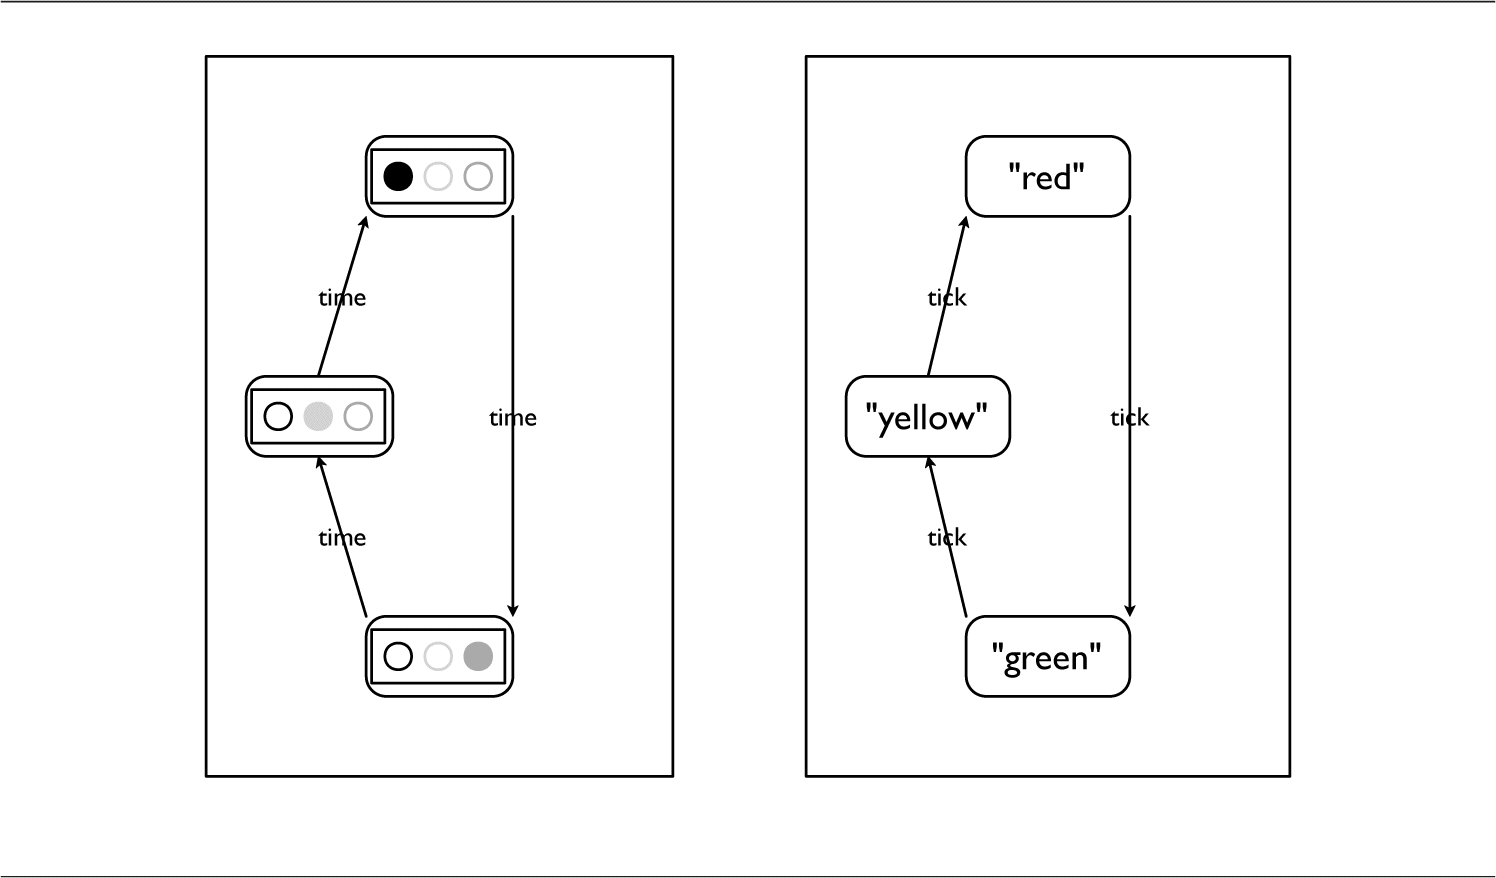
\includegraphics[width=0.7\textwidth]{images/00089.png}
  \caption{交通信号灯状态变迁图}
  \label{fig:traffic_light_fsa}
\end{figure}

图~\ref{fig:traffic_light_fsa} 显示了交通灯的状态变迁规律。每个状态由枚举定义，而状态跃迁函数 \code{tl-next} 则根据当前颜色决定下一颜色：

\begin{figure}[htbp]
  \centering
  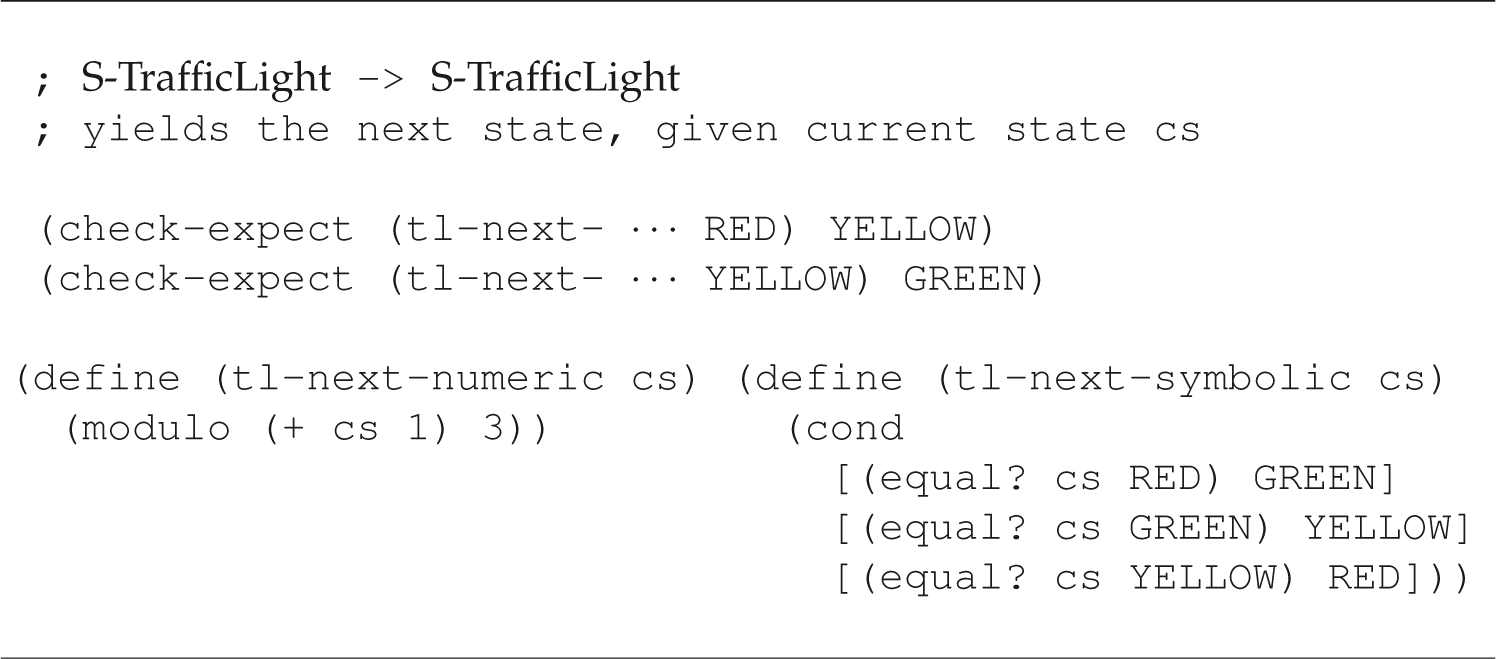
\includegraphics[width=0.85\textwidth]{images/00091.png}
  \caption{符号化交通信号灯程序定义}
  \label{fig:traffic_light_symbolic}
\end{figure}

\begin{exercise}{完善交通灯模拟程序}{59}
完成模拟交通灯状态机的世界程序设计，补全 \code{tl-render} 与 \code{tl-next} 的定义与全部测试。
\end{exercise}

\begin{exercise}{数值化交通灯状态}{60}
如果改用数值表示信号灯状态（0 表示红色，1 表示绿色，2 表示黄色），重构该程序并比较代码风格。
\end{exercise}

\begin{exercise}{使用符号常量}{61}
在数据定义与函数中使用符号常量（例如 \code{(define RED "red")}），消除程序中所有的“魔法字符串”。
\end{exercise}

\subsection{自动关门模拟程序}

考虑一个装有自动闭门器的安全防盗门。门具有三种状态：
\begin{itemize}
  \item \code{LOCKED}（已上锁）
  \item \code{CLOSED}（已关门但未上锁）
  \item \code{OPEN}（已开启）
\end{itemize}

\begin{figure}[htbp]
  \centering
  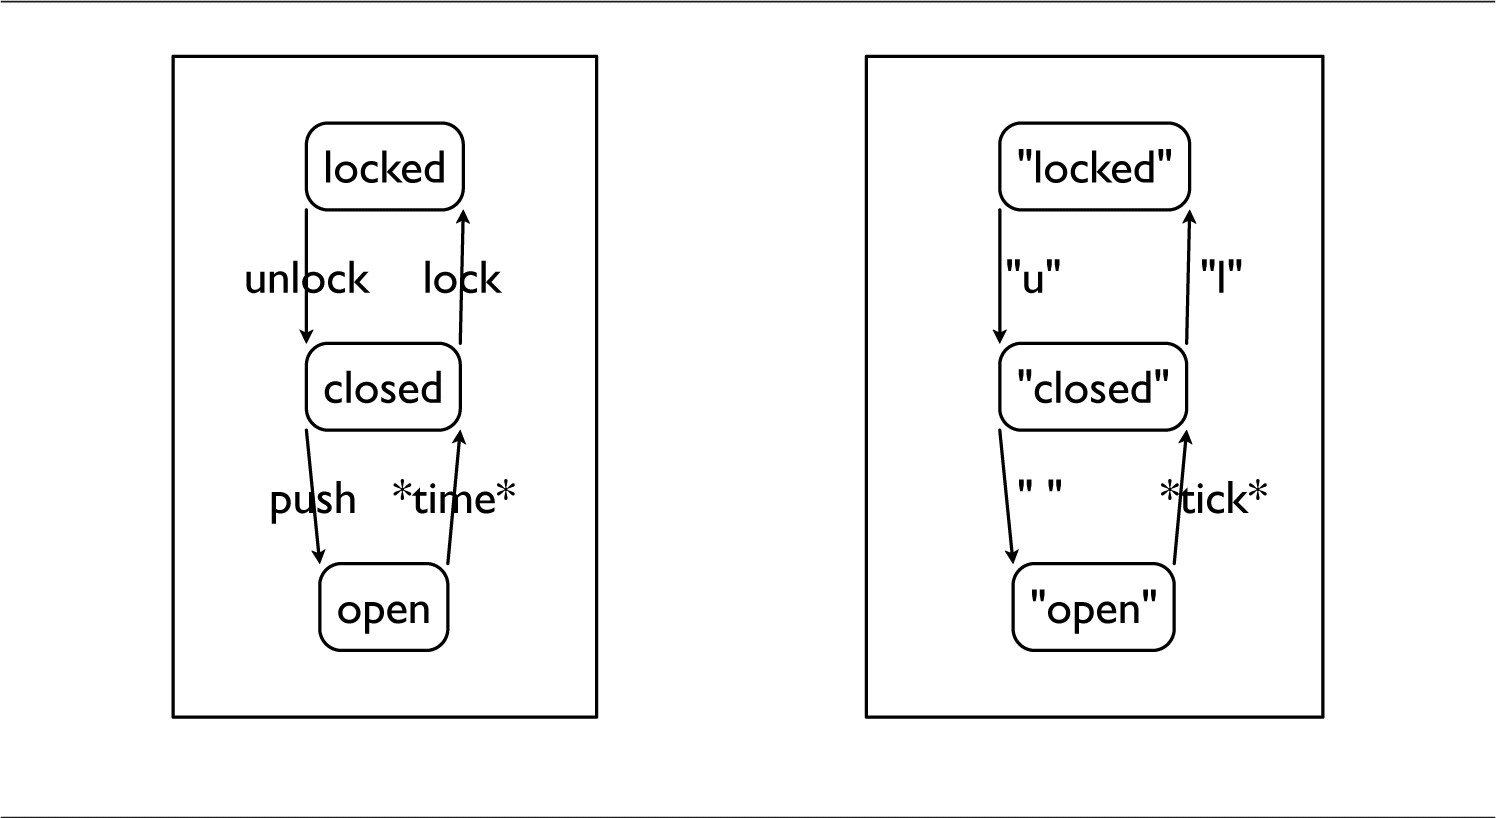
\includegraphics[width=0.75\textwidth]{images/00092.png}
  \caption{自动闭门防盗门的状态变迁图}
  \label{fig:door_fsa}
\end{figure}

如图~\ref{fig:door_fsa} 所示：
\begin{itemize}
  \item \textbf{时钟滴答（door-closer）}：自动闭门器在时钟滴答触发时将处于 \code{OPEN} 状态的门拉回 \code{CLOSED} 状态；其余状态保持不变。
  \item \textbf{按键操作（door-action）}：
    \begin{itemize}
      \item 当门处于 \code{LOCKED} 且按下 \code{"u"} 键时，门被解锁变为 \code{CLOSED}；
      \item 当门处于 \code{CLOSED} 且按下 \code{"l"} 键时，门被上锁变为 \code{LOCKED}；
      \item 当门处于 \code{CLOSED} 且按下空格键 \code{"\ "} 键时，门被推开变为 \code{OPEN}；
      \item 其余任何按键均不改变当前状态。
    \end{itemize}
\end{itemize}

我们可以将这两个函数的行为制成示例表格：

\begin{center}
\begin{tabular}{|l|l|}
\hline
\textbf{输入状态 (given state)} & \textbf{期望输出状态 (desired state)} \\
\hline
\code{LOCKED} & \code{LOCKED} \\
\code{CLOSED} & \code{CLOSED} \\
\code{OPEN}   & \code{CLOSED} \\
\hline
\end{tabular}
\end{center}

\begin{center}
\begin{tabular}{|l|l|l|}
\hline
\textbf{输入状态 (given state)} & \textbf{按键事件 (given key event)} & \textbf{期望输出状态 (desired state)} \\
\hline
\code{LOCKED} & \code{"u"} (unlock) & \code{CLOSED} \\
\code{CLOSED} & \code{"l"} (lock)   & \code{LOCKED} \\
\code{CLOSED} & \code{"\ "} (push)   & \code{OPEN} \\
\code{OPEN}   & 任意其他按键        & \code{OPEN} \\
\hline
\end{tabular}
\end{center}

\begin{figure}[htbp]
  \centering
  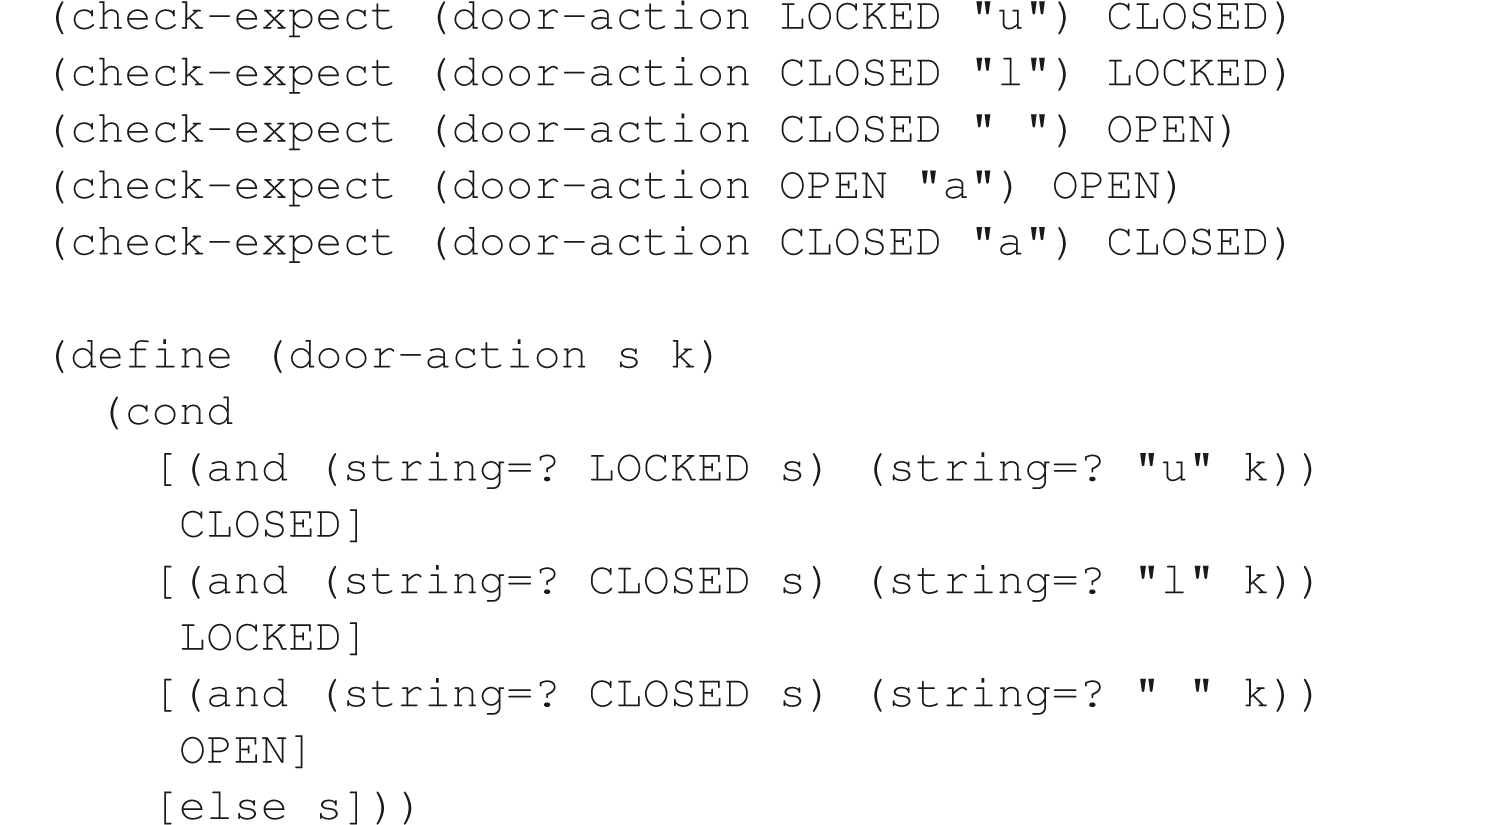
\includegraphics[width=0.85\textwidth]{images/00093.png}
  \caption{door-action 按键控制函数的实现与测试}
  \label{fig:door_closer_code}
\end{figure}

\begin{figure}[htbp]
  \centering
  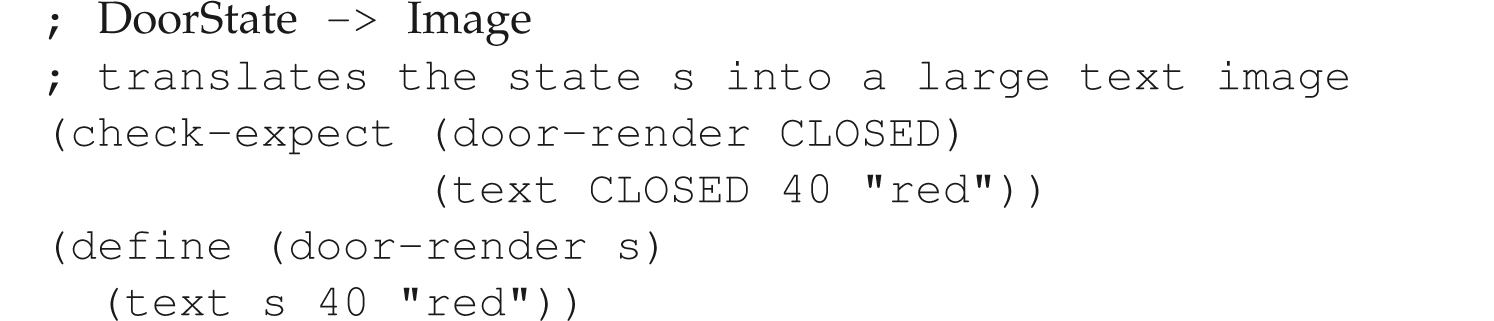
\includegraphics[width=0.85\textwidth]{images/00094.png}
  \caption{door-render 场景渲染函数的实现与测试}
  \label{fig:door_action_code}
\end{figure}

\begin{exercise}{调整仿真时钟速率}{62}
在运行防盗门模拟程序时，你可能会发现 \code{OPEN} 状态转瞬即逝（默认 1 秒有 28 个时钟滴答）。请修改 \code{door-simulation}，利用 \code{on-tick} 的时钟频率参数，使其每 3 秒才滴答一次，然后重新运行模拟并观察防盗门的开关动作。
\end{exercise}

% ==============================================================================
% 第 5 章：引入结构体 (Chapter 5: Adding Structure)
% ==============================================================================

\chapter{引入结构体}
\label{sec:ch05_structures}

在上一章中，我们学会了如何通过枚举、区间以及由它们组合而成的分类数据，对 BSL 的原始内置集合（数、字符串、图像与布尔值）施加约束。然而在现实世界中，信息往往不是单一维度的标量，而是包含多个相互关联属性的复合体。例如：
\begin{itemize}
  \item 二维平面上的一个点，同时拥有横坐标 $x$ 和纵坐标 $y$；
  \item 一只弹跳的球，不仅有当前的位置坐标，还有行进的速度与方向；
  \item 通讯录中的一条联系人记录，包含姓名、电话、电子邮件和邮寄地址。
\end{itemize}

到目前为止，我们唯一的组合手段是将两个字符串拼接成一个，或者在几何上将两幅图像叠加在一起。但在面对上述多维信息时，这些手段完全无能为力。为了优雅地将两件或两件以上的数据\term{打包}为一个单一复合实体，编程语言必须提供组合机制。在 BSL 中，这种复合数据机制被称为\term{结构体}（Structures）。

本章首先从 BSL 预定义的二维平面坐标结构体 \code{posn} 切入，剖析复合数据的核心概念与求值计算；随后介绍用户如何使用 \code{define-struct} 自定义属于自己的全新结构体类型；接着阐明结构体在数据宇宙中的定位与代数等价公理；最后给出针对结构体的完整设计配方，并将其应用于交互式图形编辑器与虚拟宠物的复杂世界程序中。

% ==============================================================================
\section{从位置到 posn 结构体}
\label{sec:5.1_from_positions_to_posn_structures}
% ==============================================================================

在解析几何中，笛卡尔平面上的每一个点都由一对实数 $(x, y)$ 唯一定位（见图~\ref{fig:cartesian_point}）。

\begin{figure}[htbp]
  \centering
  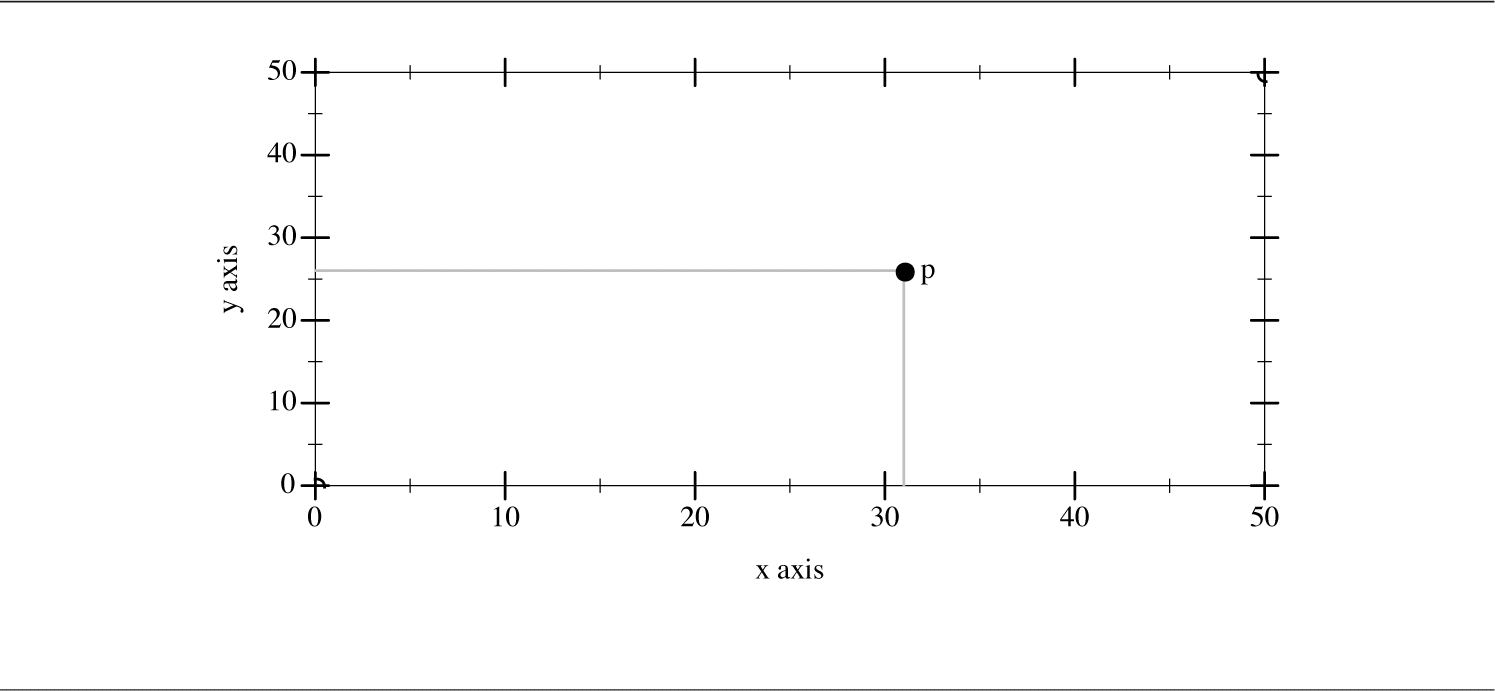
\includegraphics[width=0.45\textwidth]{images/00095.png}
  \caption{笛卡尔坐标系中的二维点 $(x, y)$}
  \label{fig:cartesian_point}
\end{figure}

为了表示这样的点，BSL 提供了一种内置的数据构造机制——\code{posn}。我们可以使用构造函数 \code{make-posn} 来创建一个位置结构体：

\begin{lstlisting}[language=BSL]
(make-posn 3 4)
(make-posn 8 6)
(make-posn 5 12)
\end{lstlisting}

在概念上，你可以把结构体想象为一个带有标签与分隔隔板的“盒子”（box）。图~\ref{fig:posn_box} 展示了 \code{(make-posn 3 4)} 在内存中的盒子模型：

\begin{figure}[htbp]
  \centering
  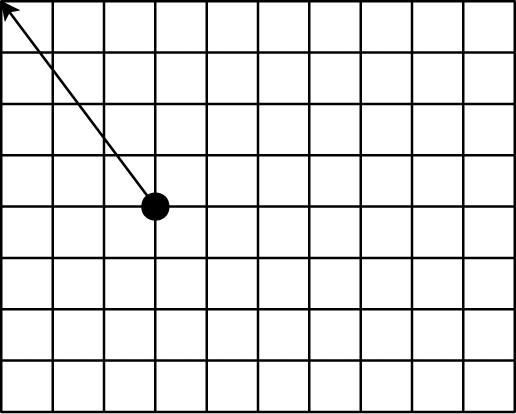
\includegraphics[width=0.35\textwidth]{images/00096.png}
  \caption{posn 结构体的盒子示意模型}
  \label{fig:posn_box}
\end{figure}

这个盒子带有标签 \code{posn}，内部包含两个插槽（slots），分别存放了横坐标 3 与纵坐标 4。

既然能将两个数装入盒子，我们就必然需要手段从盒子中取出它们。BSL 提供了两个\term{选择器}（selectors）：
\begin{itemize}
  \item \code{posn-x}：提取结构体中的 $x$ 字段；
  \item \code{posn-y}：提取结构体中的 $y$ 字段。
\end{itemize}

在 DrRacket 交互区中尝试：

\begin{replbox}
> (define p (make-posn 31 10))
> (posn-x p)
31
> (posn-y p)
10
> (posn-x (make-posn 3 4))
3
> (posn-y (make-posn 3 4))
4
\end{replbox}

选择器 \code{posn-x} 与 \code{posn-y} 就像精密的镊子，可以穿透盒子的外壳，将指定字段的数据直接提取出来。

% ==============================================================================
\section{posn 的求值与计算}
\label{sec:5.2_computing_with_posns}
% ==============================================================================

理解结构体的关键在于理解其在算术求值中的等价替换规则。针对 \code{posn}，BSL 增加了两条极其简单的归约公理：

\begin{notebox}[posn 选择器的求值规则]
对于任意两个值 $v_1$ 和 $v_2$：
\begin{align*}
\code{(posn-x (make-posn $v\_1$ $v\_2$))} &\Longrightarrow v_1 \\
\code{(posn-y (make-posn $v\_1$ $v\_2$))} &\Longrightarrow v_2
\end{align*}
也就是说，当一个选择器应用在一个显式的 \code{make-posn} 实例上时，整个表达式在一步计算内直接化简为对应槽位中的值。
\end{notebox}

例如，考虑下面表达式的求值演进：
\begin{lstlisting}[language=BSL]
  (+ (posn-x (make-posn 3 4)) (posn-y (make-posn 3 4)))
== (+ 3 (posn-y (make-posn 3 4)))
== (+ 3 4)
== 7
\end{lstlisting}

\begin{exercise}{结构体表达式手工推演}{63}
单步推演以下表达式的计算过程，写出每一步的替换结果：
\begin{lstlisting}[language=BSL]
(distance-to-0 (make-posn 3 4))
(distance-to-0 (make-posn (* 2 3) (* 2 4)))
(distance-to-0 (make-posn 12 (- 6 1)))
\end{lstlisting}
其中 \code{distance-to-0} 是计算点到原点欧几里得距离的函数：
\begin{lstlisting}[language=BSL]
(define (distance-to-0 ap)
  (sqrt (+ (sqr (posn-x ap)) (sqr (posn-y ap)))))
\end{lstlisting}
\end{exercise}

\begin{exercise}{曼哈顿距离}{64}
在曼哈顿这样的街区中，两点之间的距离不能沿对角线直飞，而必须沿着由正交街道构成的方格网格行走。一个点 $(x, y)$ 到原点 $(0, 0)$ 的\term{曼哈顿距离}（Manhattan distance）定义为：
\[
\text{ManhattanDistance}(p) = |x| + |y|
\]
设计函数 \code{manhattan-distance}，接收一个 \code{Posn} 作为输入，计算并返回其到原点的曼哈顿距离。
\end{exercise}

% ==============================================================================
\section{使用 posn 进行编程}
\label{sec:5.3_programming_with_posn}
% ==============================================================================

在程序设计配方的语境下，\code{Posn} 是一个全新的数据集合。我们要编写处理 \code{Posn} 的函数，首先必须明确其数据定义与解释：

\begin{lstlisting}[language=BSL]
; 一个 Posn 是一个结构体：
;   (make-posn Number Number)
; 解释：表示二维笛卡尔坐标系中的一个点，包含 x 坐标与 y 坐标
\end{lstlisting}

图~\ref{fig:distance_to_0_design} 展示了设计 \code{distance-to-0} 函数的完整历程：从签名、目的说明、功能测试，到针对结构体的模板，再到最终的函数体。

\begin{figure}[htbp]
  \centering
  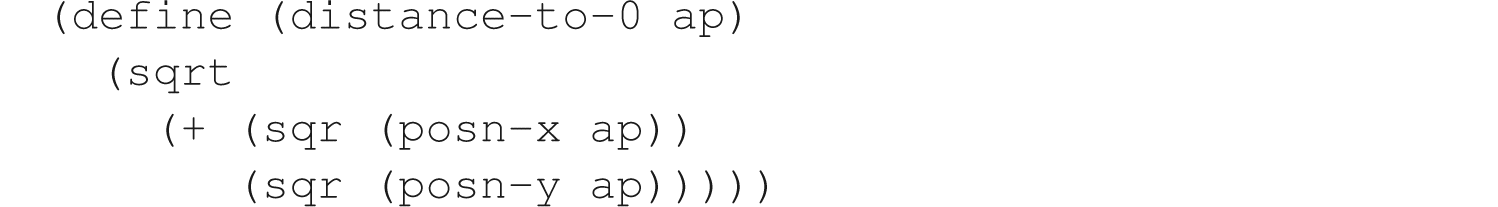
\includegraphics[width=0.85\textwidth]{images/00098.png}
  \caption{distance-to-0 函数的设计全貌与测试}
  \label{fig:distance_to_0_design}
\end{figure}

注意在编写模板时，由于输入参数 \code{ap} 是一个 \code{posn}，模板会立即写出提取其各字段的表达式：
\begin{lstlisting}[language=BSL]
(define (distance-to-0 ap)
  (... (posn-x ap) ... (posn-y ap) ...))
\end{lstlisting}
这种从数据定义直接推导模板的能力，正是设计配方的核心威力所在。

% ==============================================================================
\section{定义结构体类型}
\label{sec:5.4_defining_structure_types}
% ==============================================================================

虽然 \code{posn} 非常方便，但它只有两个字段，且语义固定为“二维坐标”。现实中的问题需要各种各样不同的复合数据：电影信息、三维向量、学生档案、颜色RGB值等。为此，BSL 赋予了程序员定义全新结构体类型的权力——\code{define-struct}。

\code{define-struct} 的通用语法形式为：

\begin{lstlisting}[language=BSL]
(define-struct StructureName [FieldName_1 ... FieldName_N])
\end{lstlisting}

例如：
\begin{lstlisting}[language=BSL]
(define-struct entry [name phone email])
\end{lstlisting}

这个单行定义施展了令人惊叹的魔法：它不是定义了一个变量，而是瞬间向 BSL 的语言环境中注入了一整套全新的函数！
对于一个拥有 $N$ 个字段的结构体类型定义：
\begin{enumerate}
  \item 一个\term{构造函数}（constructor）：名字为 \code{make-StructureName}，接收 $N$ 个参数，返回该结构体的一个新实例；
  \item $N$ 个\term{选择器}（selectors）：名字形如 \code{StructureName-FieldName\_i}，用于提取第 $i$ 个字段的值；
  \item 一个\term{类型谓词}（predicate）：名字为 \code{StructureName?}，接收任意值，判断该值是否属于此结构体类型。
\end{enumerate}

\begin{figure}[htbp]
  \centering
  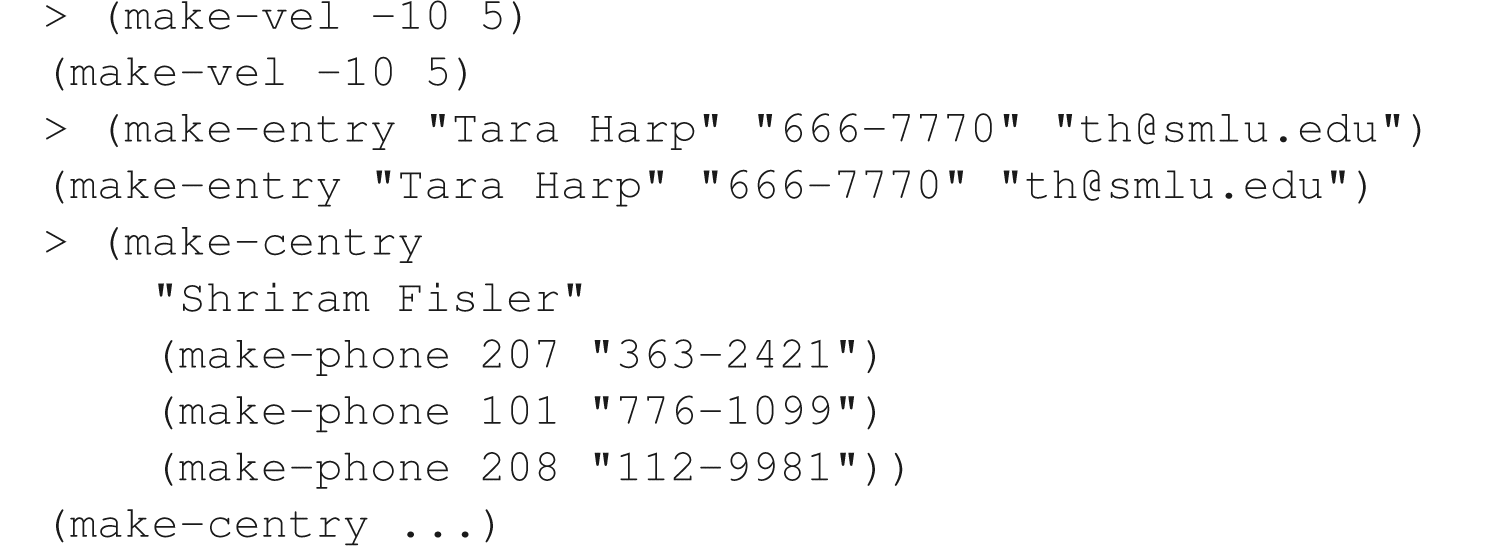
\includegraphics[width=0.75\textwidth]{images/00103.png}
  \caption{define-struct 自动派生的一组函数簇}
  \label{fig:struct_functions_derived}
\end{figure}

例如，执行 \code{(define-struct entry [name phone email])} 之后，你立刻获得了：
\begin{itemize}
  \item 构造函数：\code{make-entry}
  \item 选择器：\code{entry-name}, \code{entry-phone}, \code{entry-email}
  \item 谓词：\code{entry?}
\end{itemize}

\begin{exercise}{分析结构体类型定义}{65}
仔细研读以下结构体类型定义：
\begin{lstlisting}[language=BSL]
(define-struct movie [title director year])
(define-struct person [name hair eyes phone])
(define-struct pet [name number])
(define-struct CD [artist title price])
(define-struct sweater [material size producer])
\end{lstlisting}
分别写出每一个定义所派生出的构造函数、选择器以及类型谓词的名字和参数个数。
\end{exercise}

\begin{exercise}{创建结构体实例}{66}
回顾练习~\ref{ex:65} 中的结构体定义。对每个字段应当存放何种类型的值作出合理的推断与设计，然后为每个结构体类型至少创建一个实际的具体实例。
\end{exercise}

\begin{exercise}{弹跳球的嵌套数据表示}{67}
考虑在画布上弹跳的小球。一个小球不仅有位置，还有移动速度。这里给出一种嵌套结构表示：
\begin{lstlisting}[language=BSL]
(define-struct balld [location velocity])
(define-struct vel [deltax deltay])
\end{lstlisting}
请写出创建一个位于 $(10, 20)$、以水平速度 5 垂直速度 $-3$ 移动的小球的实例创建表达式。
\end{exercise}

\begin{exercise}{扁平化的弹跳球表示}{68}
作为对比，另一种表示法直接使用拥有四个字段的扁平结构体：
\begin{lstlisting}[language=BSL]
(define-struct ballf [x y deltax deltay])
\end{lstlisting}
创建与练习~\ref{ex:67} 相同物理含义的小球实例，并比较两种数据组织的优缺点。
\end{exercise}

% ==============================================================================
\section{使用结构体计算}
\label{sec:5.5_computing_with_structures}
% ==============================================================================

结构体实例的盒子模型同样适用于用户自定义结构体。图~\ref{fig:entry_box} 展示了 \code{entry} 结构体的内存示意图：

\begin{figure}[htbp]
  \centering
  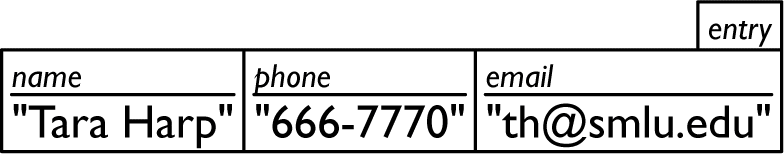
\includegraphics[width=0.65\textwidth]{images/00101.png}
  \caption{entry 结构体实例的盒子模型}
  \label{fig:entry_box}
\end{figure}

针对用户自定义结构体，BSL 的核心计算法则直接推广为：

\begin{notebox}[结构体选择器的代数公理]
设某结构体类型定义为 \code{(define-struct StructureName [f\_1 ... f\_N])}。
对于任意 $N$ 个值 $v_1, \dots, v_N$：
\[
\code{(StructureName-}f_i\code{ (make-StructureName } v_1 \code{ } \dots \code{ } v_N \code{))} \Longrightarrow v_i \quad (1 \le i \le N)
\]
此外，类型谓词满足：
\begin{align*}
\code{(StructureName? (make-StructureName } v_1 \code{ } \dots \code{ } v_N \code{))} &\Longrightarrow \code{\#true} \\
\code{(StructureName? } \text{other-value} \code{)} &\Longrightarrow \code{\#false}
\end{align*}
\end{notebox}

\begin{exercise}{绘制盒子图}{69}
为你在练习~\ref{ex:66} 中创建的所有结构体实例绘制类似图~\ref{fig:entry_box} 的盒子示意图。
\end{exercise}

\begin{exercise}{写出代数公理}{70}
为以下两个结构体类型分别完整列出其选择器和谓词的代数计算公理：
\begin{lstlisting}[language=BSL]
(define-struct centry [name home office cell])
(define-struct phone [area number])
\end{lstlisting}
\end{exercise}

\begin{exercise}{结构体字段访问求值验证}{71}
在 DrRacket 定义区输入以下定义，然后预测并在交互区验证输出结果：
\begin{lstlisting}[language=BSL]
(define-struct posn [x y]) ; 注意：BSL 内置了 posn，无需重复定义
(define p1 (make-posn 2 3))
(define p2 (make-posn (posn-y p1) (posn-x p1)))
\end{lstlisting}
预测 \code{(posn-x p2)} 与 \code{(posn-y p2)} 的计算结果。
\end{exercise}

% ==============================================================================
\section{结构体编程}
\label{sec:5.6_programming_with_structures}
% ==============================================================================

在实际业务中，我们经常需要对结构体进行“更新”（update）。请牢记：\textbf{在函数式编程中，数据是不可变的（immutable）}。所谓“更新”一个点，绝不是去修改原有点的字段，而是根据旧点的值计算出一个\textbf{全新的结构体实例}！

例如，设计一个函数 \code{posn-up-x}，它接收一个点 \code{p} 和一个新坐标 \code{n}，返回一个横坐标为 \code{n}、纵坐标保持与 \code{p} 相同的新点：

\begin{lstlisting}[language=BSL]
; Posn Number -> Posn
; 生成一个新的 Posn，其 x 坐标为 n，y 坐标取自 p
(check-expect (posn-up-x (make-posn 3 4) 10) (make-posn 10 4))

(define (posn-up-x p n)
  (make-posn n (posn-y p)))
\end{lstlisting}

\begin{exercise}{电话结构体数据定义}{72}
为如下三字段电话号码设计数据定义与解释：
\begin{lstlisting}[language=BSL]
(define-struct phone\# [area switch num])
\end{lstlisting}
并给出三个具体的电话号码数据实例。
\end{exercise}

\begin{exercise}{点更新函数 posn-up-x}{73}
完整实现并测试 \code{posn-up-x} 函数，确保其通过所有单元测试。
\end{exercise}

\begin{exercise}{红点点击世界程序}{74}
编写一个世界程序，其世界状态为一个 \code{Posn}。画布初始时在 $(0, 0)$ 处绘制一个半径为 3 的红点；当用户在画布上点击鼠标时，红点立即跃迁到鼠标点击的坐标位置。
\end{exercise}

\begin{exercise}{UFO 移动函数}{75}
设计函数 \code{ufo-move}，接收一个表示当前位置的 \code{Posn} 和表示速度的 \code{Vel} 结构体，返回下一时刻小球的新位置 \code{Posn}。
\end{exercise}

% ==============================================================================
\section{数据的全集与领域}
\label{sec:5.7_the_universe_of_data}
% ==============================================================================

当我们引入结构体之后，程序中所处理的数据世界发生了根本性的飞跃。

在图~\ref{fig:universe_simple} 中，原始数据宇宙只包含离散的基本类型原子（数、字符串、图像、布尔值）。

\begin{figure}[htbp]
  \centering
  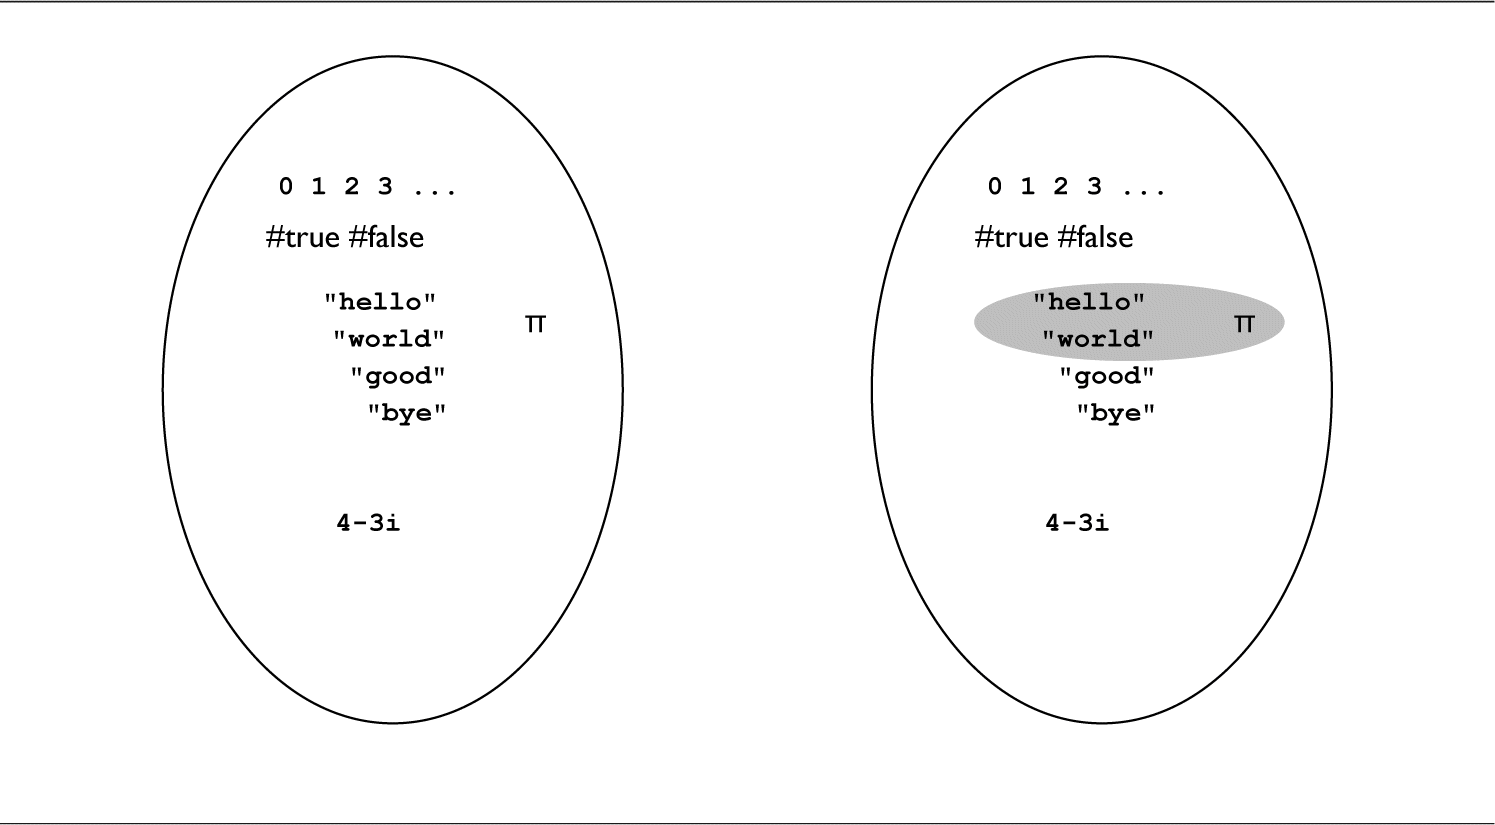
\includegraphics[width=0.65\textwidth]{images/00107.png}
  \caption{原始的基本数据全集}
  \label{fig:universe_simple}
\end{figure}

而每当我们在程序中书写一行 \code{(define-struct S [f\_1 ... f\_N])}，数据宇宙中就立即诞生了一个全新的、无限庞大的星系（见图~\ref{fig:universe_with_structs}）——所有由 \code{make-S} 生成的实例构成了一个全新的数据子集！

\begin{figure}[htbp]
  \centering
  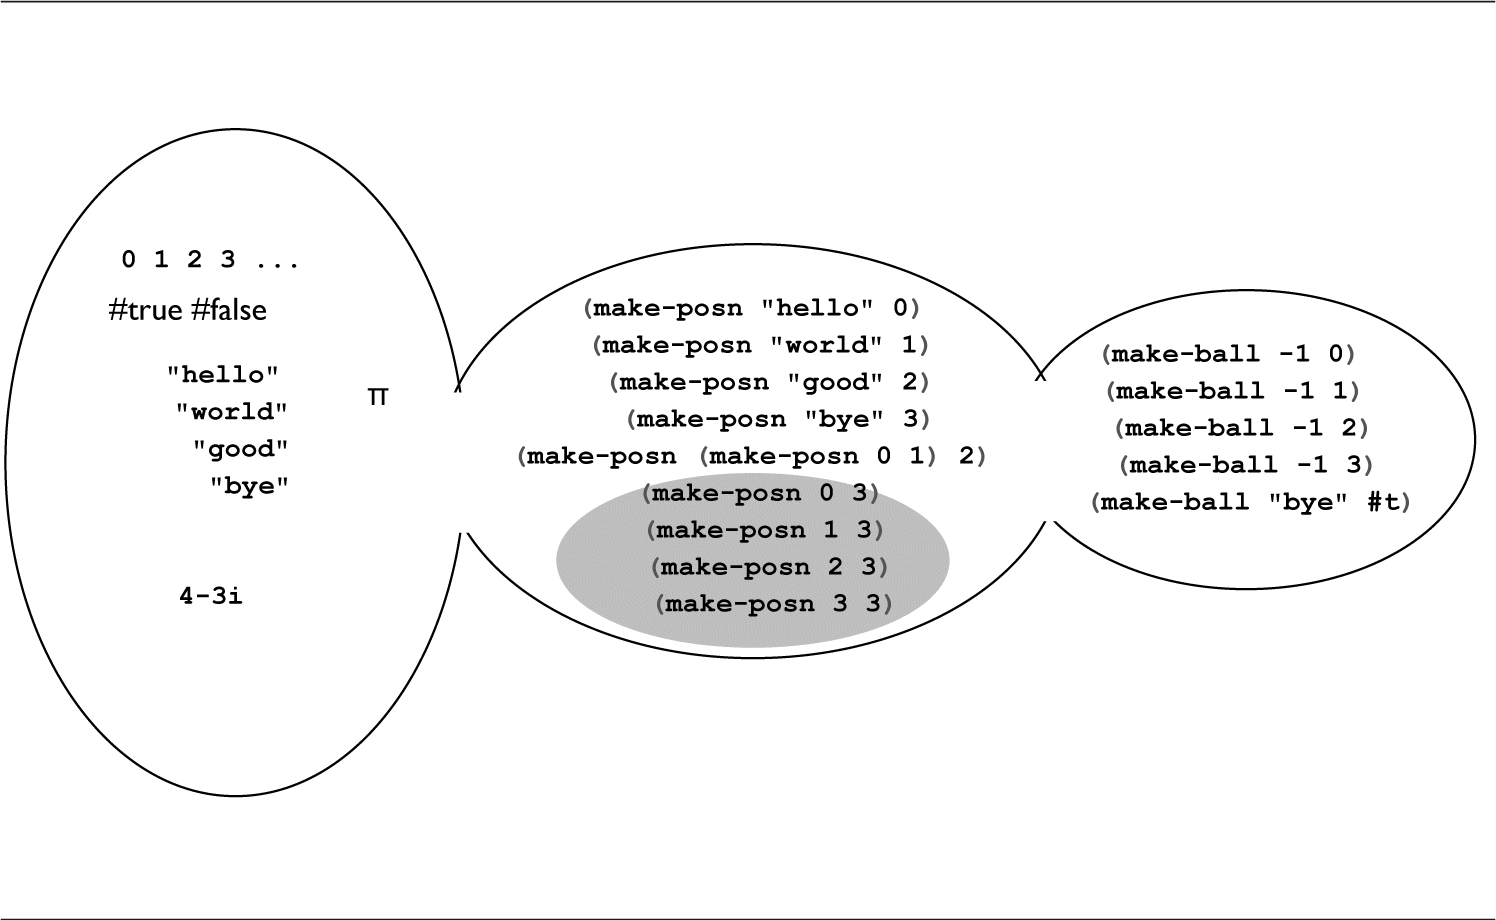
\includegraphics[width=0.7\textwidth]{images/00108.png}
  \caption{引入结构体后无限膨胀的数据宇宙}
  \label{fig:universe_with_structs}
\end{figure}

更令人惊叹的是：由于结构体的字段本身又可以存放任意数据值（包括另一个结构体实例！），我们获得了无限层级嵌套与组合复杂世界现实的能力。

\begin{exercise}{为结构体写出严密的数据定义}{76}
回顾练习~\ref{ex:65} 中的结构体定义（movie, person, pet, CD, sweater）。为每一个结构体类型写出规范的、包含各字段类型约束与物理现实解释的数据定义。
\end{exercise}

\begin{exercise}{时间结构体}{77}
提供一个结构体类型定义与数据定义，用于精确表示自午夜（00:00:00）以来经过的时间（包含小时、分钟和秒）。
\end{exercise}

\begin{exercise}{三字母单词结构体}{78}
定义一个表示由三个字母组成的单词的结构体类型定义及数据定义。
\end{exercise}

\begin{exercise}{复杂场景数据表示}{79}
为以下实体分别设计结构体与数据定义：
\begin{enumerate}
  \item 屏幕上彩色的几何图形；
  \item 包含姓名、年龄、住址的个人档案；
  \item 包含品种、晶片编号、疫苗注射状态的宠物犬；
  \item 具有弹药量、伤害值和耐久度的武器。
\end{enumerate}
\end{exercise}

% ==============================================================================
\section{针对结构体的设计配方}
\label{sec:5.8_designing_with_structures}
% ==============================================================================

当函数的输入参数包含结构体时，程序设计配方展现出极其清晰的形式化指引：

\begin{recipebox}{设计处理结构体的函数}
\begin{enumerate}
  \item \textbf{数据定义}：
    \begin{itemize}
      \item 使用 \code{(define-struct TypeName [f\_1 ... f\_N])} 定义结构体形态；
      \item 编写对应的数据定义注释，明确指定每个字段的类型取值范围；
      \item 给出每个字段在现实世界中的业务解释（Interpretation）。
    \end{itemize}
  \item \textbf{签名、目的说明与函数头}：在签名中以自定义结构体名称（首字母大写，如 \code{Posn}, \code{Entry}）作为输入或输出类型。
  \item \textbf{功能示例}：在创建示例时，必须使用构造函数 \code{make-TypeName} 实例化具体的数据对象。
  \item \textbf{函数模板}：\textbf{对于结构体参数，无条件提取所有选择器！}
\begin{lstlisting}[language=BSL]
(define (fn-for-struct s)
  (... (TypeName-f_1 s) ...
   ... (TypeName-f_2 s) ...
   ...
   ... (TypeName-f_N s) ...))
\end{lstlisting}
    模板忠实反映了“盒子”里的每一个插槽。你在写函数体之前，就已经清楚拥有了哪些现成的零件。
  \item \textbf{函数体实现}：利用提取出的各字段数据，组合出最终的运算结果。若输出也是结构体，则调用相应的构造函数生成新实例。
  \item \textbf{自动化测试}：使用 \code{check-expect} 校验所有测试用例。
\end{enumerate}
\end{recipebox}

\begin{exercise}{写出结构体模板}{80}
为练习~\ref{ex:65} 中的五个结构体类型分别写出其标准处理函数的函数模板。
\end{exercise}

\begin{exercise}{时间转秒数}{81}
设计函数 \code{time->seconds}，接收一个练习~\ref{ex:77} 中定义的时间结构体，计算并返回自午夜以来累计流逝的总秒数。
\end{exercise}

\begin{exercise}{三字母单词匹配}{82}
设计函数 \code{compare-word}，接收两个练习~\ref{ex:78} 中定义的三字母单词结构体，逐个字母比对并返回一个指示每个位置是否匹配的新单词结构体。
\end{exercise}

% ==============================================================================
\section{世界程序中的结构体}
\label{sec:5.9_structure_in_the_world}
% ==============================================================================

在第 3 章中，世界程序的 WorldState 只能是一个单一标量（数或字符串）。现在有了结构体，世界状态可以同时追踪任意多个运动物体或环境参数！

例如，如果一个太空射击游戏同时包含飞船坐标、外星人飞碟坐标以及发射出的导弹坐标，我们只需定义：
\begin{lstlisting}[language=BSL]
(define-struct space-game [ship ufo missile])
\end{lstlisting}
世界状态在每一帧时钟滴答中被整体更新，渲染函数则从各个字段中分别提取坐标进行分层绘制。

% ==============================================================================
\section{图形文本编辑器}
\label{sec:5.10_a_graphical_editor}
% ==============================================================================

作为结构体威力的绝佳展示，我们来设计一个单行交互式图形文本编辑器（Graphical Text Editor）！

编辑器展现为一个输入框，包含一段文字和一个垂直光标。用户在键盘上输入字母时，字符插入到光标所在位置；按退格键（\code{"\textbackslash b"}）时删除光标左侧的字符；按左方向键（\code{"left"}）或右方向键（\code{"right"}）时光标左右移动。

如何用数据表示这个编辑器呢？
直觉上，你可能会想用一个长字符串加一个光标索引数字（Index）。但处理字符串切片和索引加减极易出现“差一错误”（off-by-one error）。
HtDP 传授了一个精妙绝伦的数据表示——\textbf{将文本按光标拆分为两段字符串}（见图~\ref{fig:editor_split}）：
\begin{itemize}
  \item \code{pre}：光标左侧的所有文本；
  \item \code{post}：光标右侧的所有文本。
\end{itemize}

\begin{figure}[htbp]
  \centering
  
\includegraphics[width=0.7\textwidth]{images/00110.png}
  \caption{光标切分文本模型示意图}
  \label{fig:editor_split}
\end{figure}

\begin{lstlisting}[language=BSL]
(define-struct editor [pre post])
; 一个 Editor 是一个结构体：
;   (make-editor String String)
; 解释：(make-editor s t) 表示光标位于字符串 s 和 t 之间
\end{lstlisting}

例如：\code{(make-editor "hello " "world")} 表示文本为 \code{"hello world"}，光标位于空格与 \code{"w"} 之间。

\begin{figure}[htbp]
  \centering
  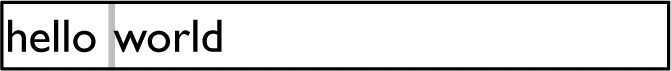
\includegraphics[width=0.45\textwidth]{images/00111.png}
  \caption{editor 结构体实例的盒子模型}
  \label{fig:editor_box}
\end{figure}

\begin{figure}[htbp]
  \centering
  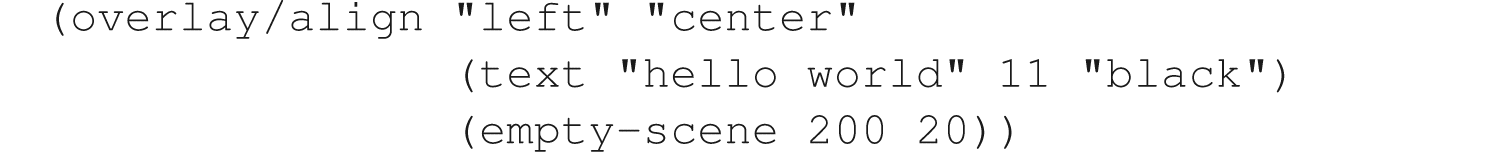
\includegraphics[width=0.85\textwidth]{images/00112.png}
  \caption{文本编辑器的渲染函数 render}
  \label{fig:editor_render}
\end{figure}

\begin{exercise}{编辑器渲染函数}{83}
设计函数 \code{render}，接收一个 \code{Editor}，生成包含文本与垂直红色光标线段的图像（如图~\ref{fig:editor_render} 所示）。
\end{exercise}

\begin{exercise}{按键编辑逻辑 edit}{84}
设计函数 \code{edit}，接收一个 \code{Editor} 和一个 \code{KeyEvent}，返回更新后的 \code{Editor}。必须严谨处理以下情况：
\begin{itemize}
  \item 普通单字符按键（长度为 1 的非控制字符串）：追加到 \code{pre} 的末尾；
  \item \code{"\textbackslash b"}（退格）：删除 \code{pre} 的最后一个字符；若 \code{pre} 为空则忽略；
  \item \code{"left"}（左移光标）：将 \code{pre} 的最后一个字符转移到 \code{post} 的开头；
  \item \code{"right"}（右移光标）：将 \code{post} 的首字符转移到 \code{pre} 的末尾；
  \item \code{"\textbackslash t"} 或 \code{"\textbackslash r"} 等控制字符：直接忽略，保持原样。
\end{itemize}
\end{exercise}

\begin{exercise}{组装运行图形编辑器}{85}
编写 \code{run} 函数，接收一个初始文本字符串，调用 \code{big-bang} 启动交互式文本编辑器！
\end{exercise}

\begin{exercise}{防止文本超出边界}{86}
如果用户持续输入，文本可能会超出画布边界。修改 \code{edit} 函数，若新字符会导致文本宽度超出画布，则拒绝输入。
\end{exercise}

\begin{exercise}{基于字符串与索引的替代实现}{87}
尝试使用第一种思路（一个完整字符串加一个整数光标索引）重做上述编辑器练习，对比两套方案的实现复杂度与代码优雅性。
\end{exercise}

% ==============================================================================
\section{更多虚拟宠物}
\label{sec:5.11_more_virtual_pets}
% ==============================================================================

在第 3.7 节中，我们分别独立编写了行走的小猫世界程序与心情计世界程序。现在借助结构体，我们可以将它们合二为一，打造一个真正鲜活的虚拟宠物！

\begin{figure}[htbp]
  \centering
  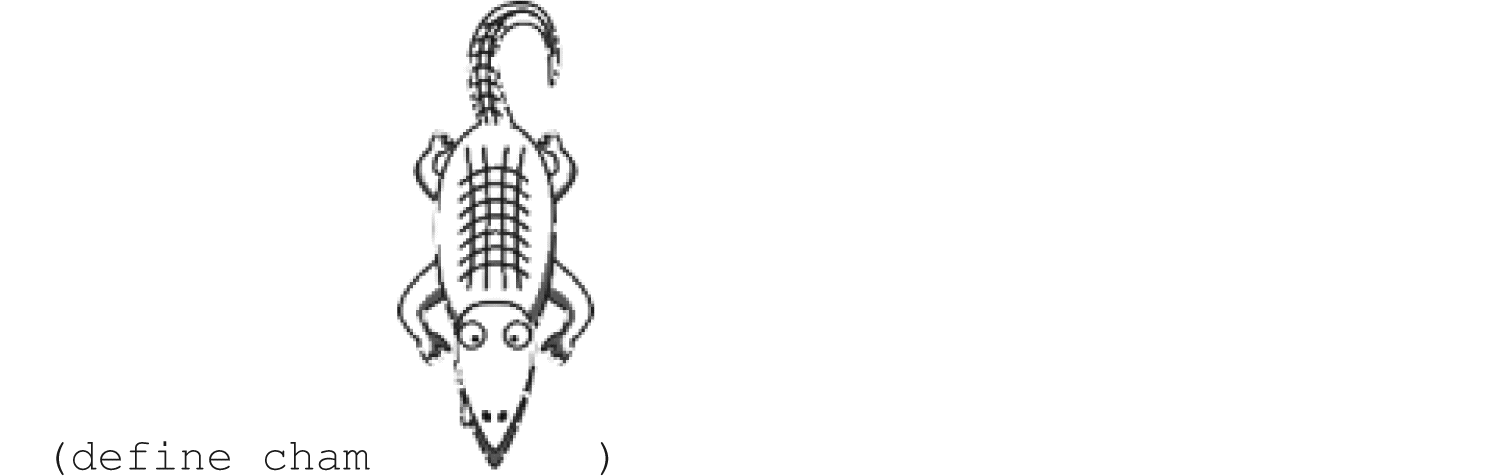
\includegraphics[width=0.6\textwidth]{images/00113.png}\\[1ex]
  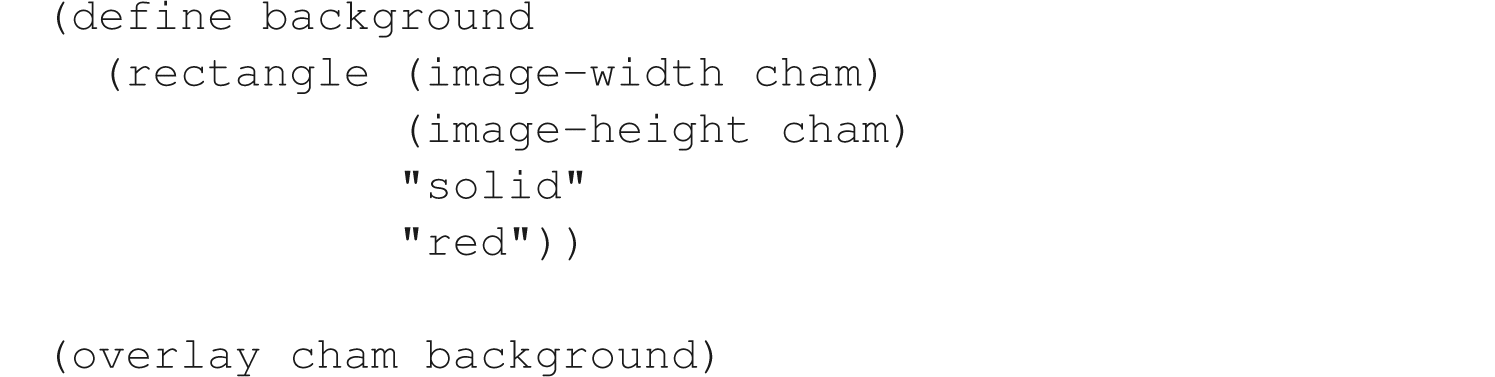
\includegraphics[width=0.6\textwidth]{images/00114.png}
  \caption{行走的小猫（上）与快乐指数仪表盘（下）}
  \label{fig:cat_and_gauge}
\end{figure}

\begin{exercise}{虚拟小猫的数据定义 VCat}{88}
定义一个结构体类型与数据定义 \code{VCat}，同时记录小猫的水平坐标 $x$ 与当前的快乐值 $h$。
\end{exercise}

\begin{exercise}{打造 happy-cat 世界程序}{89}
设计 \code{happy-cat} 程序，在画布上方显示小猫，下方显示心情指数进度条。小猫每前进一步，心情便略微下滑；用户可以通过喂食（下方向键）或抚摸（上方向键）来提升小猫的快乐值。
\end{exercise}

\begin{exercise}{停止条件：猫咪伤心过度}{90}
利用 \code{stop-when} 子句，当小猫的快乐值跌落至 0 时立即终止程序。
\end{exercise}

\begin{exercise}{双向行走的猫咪}{91}
扩展 \code{VCat} 结构体以记录移动方向。当小猫触碰画布边缘时，自动掉头向反方向行走。
\end{exercise}

\begin{figure}[htbp]
  \centering
  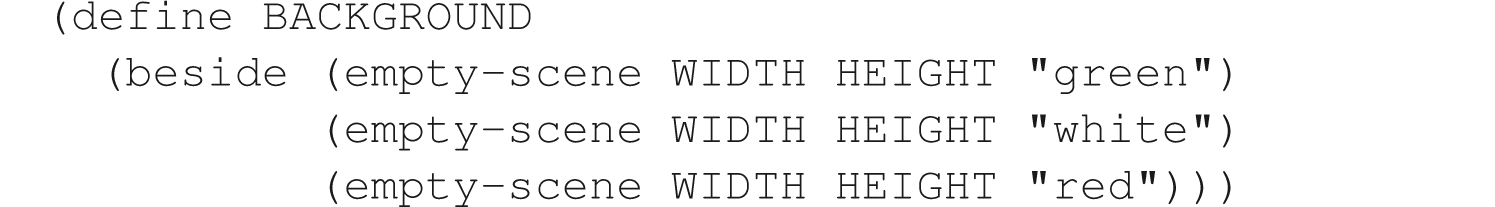
\includegraphics[width=0.7\textwidth]{images/00115.png}
  \caption{三色背景上行走的变色龙}
  \label{fig:cham_tricolor}
\end{figure}

\begin{exercise}{变色龙虚拟宠物}{92}
设计 \code{cham} 虚拟变色龙程序。变色龙从左至右在画布上漫步，同样拥有饥饿与快乐机制。
\end{exercise}

\begin{exercise}{三色背景上的变色龙}{93}
复制并修改练习~\ref{ex:92} 的程序，使得变色龙行走在一个由红、白、绿三色竖条纹构成的背景上，并且身体颜色会随着按键改变。
\end{exercise}

% ==============================================================================
% 第 6 章：分类与结构体 (Chapter 6: Itemizations and Structures)
% ==============================================================================

\chapter{分类与结构体}
\label{sec:ch06_itemizations}

在第 4 章中，我们学习了\term{分类数据}（Itemizations），它通过将离散的原子值（如字符串标签）和连续的范围（如数值区间）组合在一起来描述复杂情况。在第 5 章中，我们学习了\term{结构体}（Structures），它允许我们将多项相互关联的数据打包为一个单一的复合实体。

本章将这两大核心概念融合在一起：\textbf{带有结构体的分类数据}。在实际软件工程中，这种组合模式无处不在。一个系统在不同阶段可能处于截然不同的状态模式，而每种状态模式所需追踪的复合属性也大相径庭。例如在视频游戏中，玩家在未发射子弹前只需记录飞船位置，发射子弹后则必须同时追踪飞船与子弹的位置。

此外，本章还将系统性地探讨\term{输入验证}（防御性设计）、\term{世界状态谓词}以及\term{相等性比较谓词}，使我们的程序不仅结构严谨，更具备工业级的鲁棒性。

% ==============================================================================
\section{再论分类数据的设计}
\label{sec:6.1_designing_with_itemizations_again}
% ==============================================================================

为了掌握带有结构体的分类数据设计，我们将深入开发一个经典的街机游戏——\term{太空侵略者}（Space Invaders）。

在游戏中，一架不明飞行物（UFO）自天顶向地面降落，地面上一辆坦克（Tank）左右移动并伺机发射一枚反击导弹（Missile）。游戏存在两个截然不同的状态阶段：
\begin{enumerate}
  \item \textbf{瞄准阶段（Aiming）}：导弹尚未发射，装载在坦克上；
  \item \textbf{发射阶段（Fired）}：导弹已点火发射，正垂直向天空疾驰。
\end{enumerate}

\begin{figure}[htbp]
  \centering
  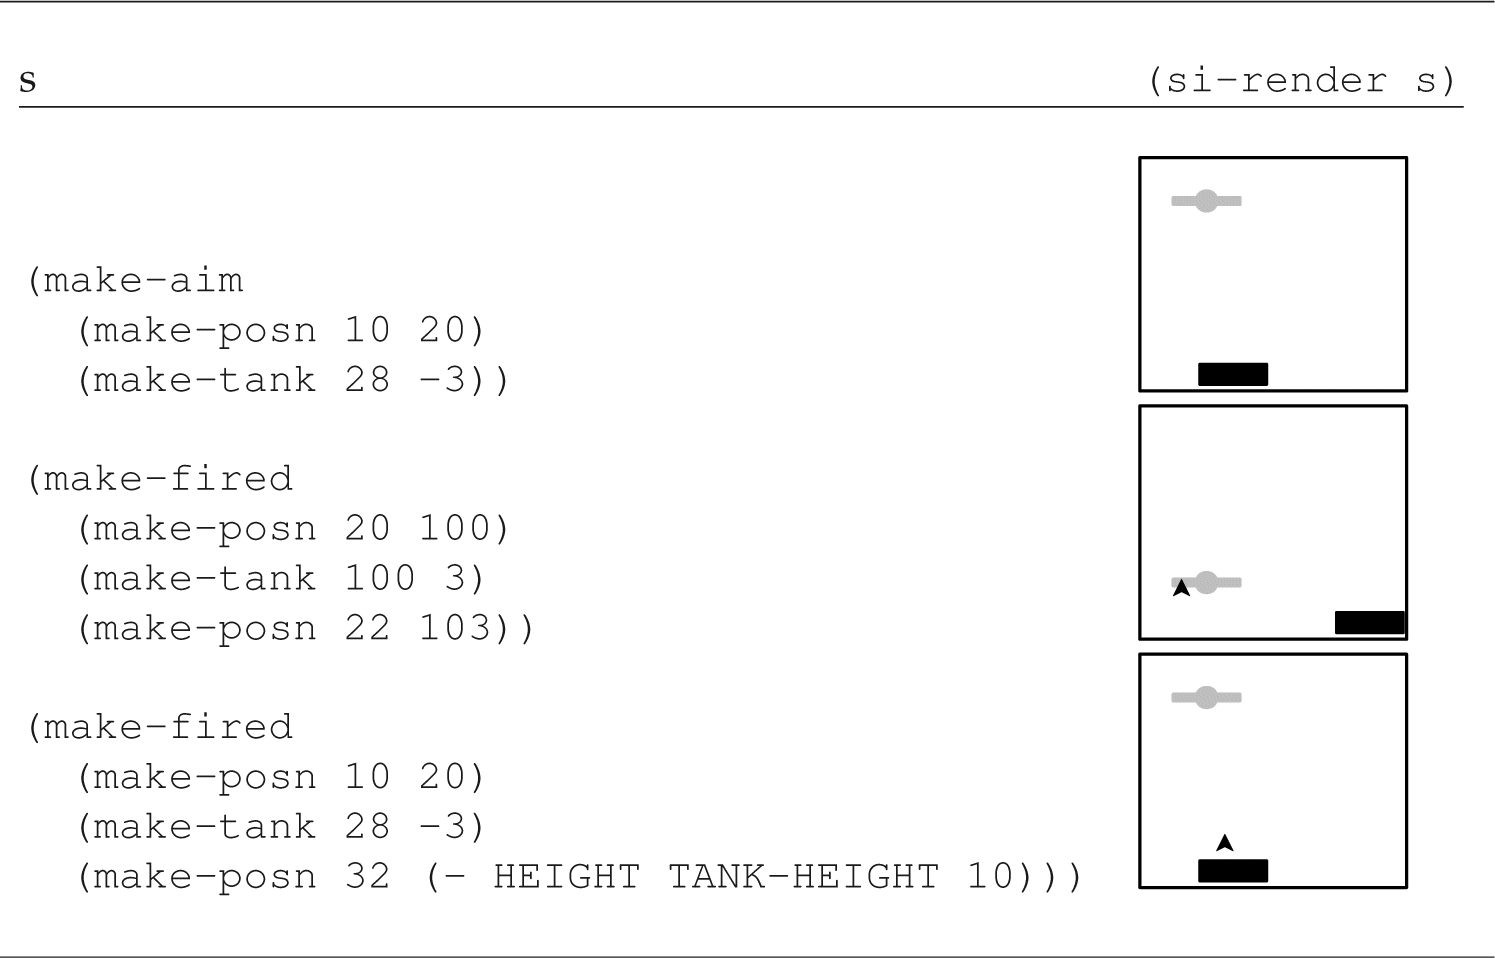
\includegraphics[width=0.75\textwidth]{images/00118.png}
  \caption{太空侵略者游戏状态渲染示例}
  \label{fig:space_invader_render_examples}
\end{figure}

针对这两个状态分支，我们定义两个专属的结构体：

\begin{lstlisting}[language=BSL]
(define-struct aim [ufo tank])
(define-struct fired [ufo tank missile])
\end{lstlisting}

进而定义游戏状态分类数据 \code{SIGS}（Space Invader Game State）：

\begin{lstlisting}[language=BSL]
; 一个 SIGS (太空侵略者游戏状态) 是以下两者之一：
; -- (make-aim Posn Tank)
; -- (make-fired Posn Tank Posn)
; 解释：表示游戏处于“未发射导弹”或“导弹已发射”状态。
; 其中 Posn 表示 UFO 或导弹在画布上的坐标；
; Tank 记录坦克的水平位置与移动速度。
\end{lstlisting}

\begin{figure}[htbp]
  \centering
  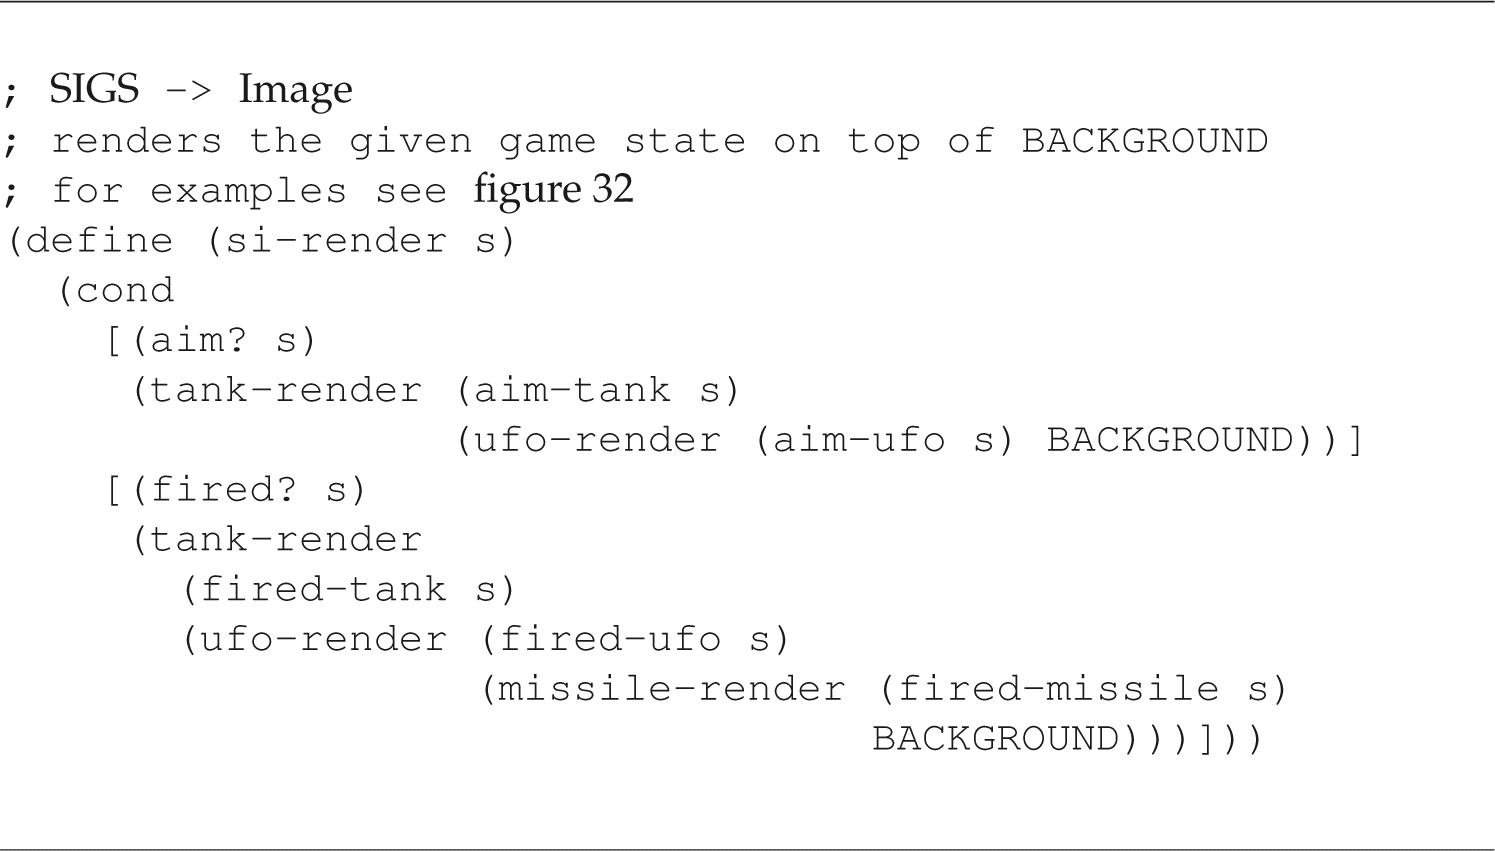
\includegraphics[width=0.85\textwidth]{images/00122.png}
  \caption{包含结构体的完整渲染函数 si-render（注：代码注释中原书连续编号 Figure 32 对应本书图 6.2）}
  \label{fig:sigs_render_full}
\end{figure}

观察图~\ref{fig:sigs_render_full} 中的 \code{si-render} 函数。由于输入参数 \code{s} 是一个分类数据，函数顶层由一个 \code{cond} 表达式统领，分别利用谓词 \code{aim?} 与 \code{fired?} 区分具体属于哪种结构体；在每个分支内部，则严格遵循结构体设计配方，提取各字段选择器进行下层图像合成。

\begin{exercise}{游戏场景与常数设计}{94}
绘制太空侵略者游戏在不同阶段的若干场景草图。据此确定游戏中的不变常数与可变量：定义画布尺寸常数（\code{WIDTH}, \code{HEIGHT}）、UFO 图像、坦克图像、导弹图像以及背景画布 \code{BACKGROUND}。
\end{exercise}

\begin{exercise}{分析游戏状态实例}{95}
解释为什么以下三个实例分别属于数据定义的第一个或第二个分支：
\begin{lstlisting}[language=BSL]
(make-aim (make-posn 20 10) (make-tank 28 -3))
(make-fired (make-posn 20 10) (make-tank 28 -3) (make-posn 28 (- HEIGHT TANK-HEIGHT)))
(make-fired (make-posn 20 100) (make-tank 100 3) (make-posn 22 103))
\end{lstlisting}
\end{exercise}

\begin{exercise}{绘制游戏场景草图}{96}
在 $200 \times 200$ 的画布坐标系中，手动绘制练习~\ref{ex:95} 中三个状态分别对应的游戏渲染画面。
\end{exercise}

\begin{exercise}{设计分层渲染辅助函数}{97}
遵循辅助函数设计原则，分别设计 \code{tank-render}、\code{ufo-render} 与 \code{missile-render}，并用它们装配出高内聚、低耦合的 \code{si-render}。
\end{exercise}

\begin{exercise}{胜负终止判断 si-game-over?}{98}
设计游戏结束判断函数 \code{si-game-over?}。游戏在发生以下任一情况时终止：
\begin{enumerate}
  \item UFO 触地着陆（即其纵坐标达到或超过 \code{HEIGHT}）；
  \item 导弹成功命中 UFO（即导弹坐标与 UFO 坐标距离足够接近，例如小于 5 像素）。
\end{enumerate}
此外，设计游戏终盘画面渲染函数 \code{si-render-final}，在屏幕上醒目展示游戏结果。
\end{exercise}

\begin{exercise}{移动更新函数 si-move}{99}
设计时钟滴答处理函数 \code{si-move}：
\begin{itemize}
  \item 坦克沿水平方向以当前速度匀速移动；
  \item 导弹（若已发射）垂直向上高速直线运动；
  \item UFO 垂直匀速下落，并在水平方向进行小幅随机跳跃（借助 BSL 内置的 \code{random} 函数）。
\end{itemize}
\end{exercise}

\begin{exercise}{按键控制函数 si-control}{100}
设计按键事件处理函数 \code{si-control}，响应以下三颗按键：
\begin{itemize}
  \item \code{"left"}：改变坦克速度方向向左；
  \item \code{"right"}：改变坦克速度方向向右；
  \item 空格键 \code{"\ "}：若导弹尚未发射，则在坦克顶部点火生成一枚新导弹！若导弹已在飞行中，则忽略此按键。
\end{itemize}
\end{exercise}

\begin{exercise}{自动化测试全覆盖}{101}
将图~\ref{fig:space_invader_render_examples} 与图~\ref{fig:sigs_render_full} 中的示例转化为严格的 \code{check-expect} 单元测试。
\end{exercise}

\subsection{另一种数据表示方案：单一结构体与可选字段}

作为对比，我们也可以将游戏状态建模为一个包含三字段的统一结构体：

\begin{lstlisting}[language=BSL]
(define-struct sigs [ufo tank missile])
; 一个 SIGS.v2 是一个结构体：
;   (make-sigs Posn Tank MissileOrNot)
; 一个 MissileOrNot 是以下两者之一：
; -- #false
; -- Posn
; 解释：#false 表示尚未发射导弹；Posn 表示导弹当前坐标
\end{lstlisting}

\begin{figure}[htbp]
  \centering
  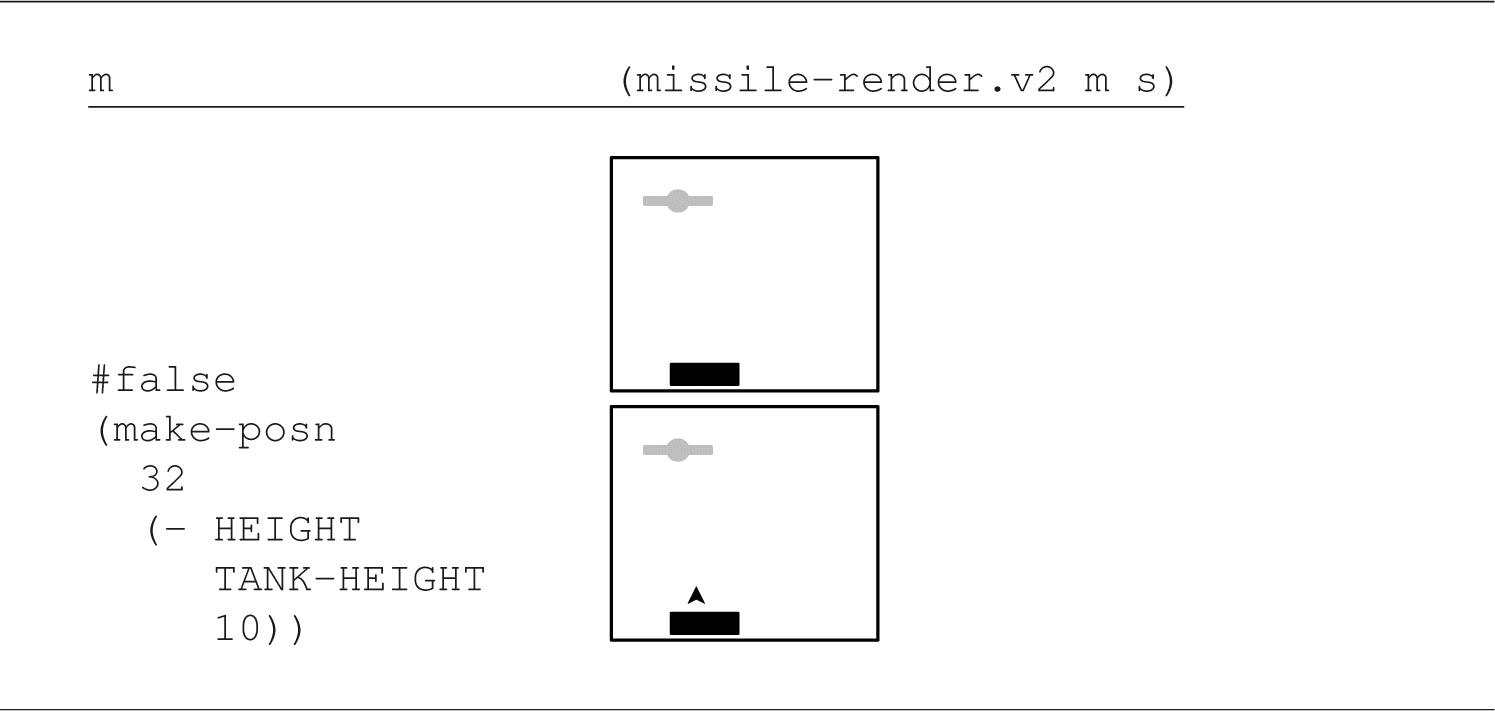
\includegraphics[width=0.85\textwidth]{images/00126.png}
  \caption{第二种游戏状态数据表示下的渲染函数}
  \label{fig:sigs_v2_render}
\end{figure}

\begin{exercise}{完成第二种方案的代码}{102}
基于 \code{SIGS.v2} 数据表示，重新设计太空侵略者游戏的所有核心事件处理函数。
\end{exercise}

\begin{exercise}{动物园管理系统}{103}
设计一套结构体与分类数据，用于表示动物园中的四种动物：蜘蛛（记录剩余腿数与运输体积）、大象（记录空间需求）、蟒蛇（记录长度与腰围）和犰狳（记录体重与铠甲硬度）。设计函数 \code{fits?} 判断某只动物是否能装入给定制式的笼子。
\end{exercise}

\begin{exercise}{车辆分类系统}{104}
为包含小汽车、货车、大巴和 SUV 的车队设计结构体与分类数据定义，并编写函数计算过路费。
\end{exercise}

\begin{exercise}{广义坐标 Coordinate}{105}
考虑如下数据定义：
\begin{lstlisting}[language=BSL]
; 一个 Coordinate 是以下两者之一：
; -- 一个非负数 Number
; -- 一个 Posn
; 解释：单个数字表示位于数轴上的点；Posn 表示平面二维点
\end{lstlisting}
设计函数 \code{distance-to-origin}，计算任意 \code{Coordinate} 到坐标原点的欧几里得距离。
\end{exercise}

% ==============================================================================
\section{混合型世界程序}
\label{sec:6.2_mixing_up_worlds}
% ==============================================================================

在第 5.11 节中，我们分别设计了小猫与变色龙。如果我们希望在一个程序中让用户自主选择领养哪种宠物，世界状态本身就必须是一个分类数据！

\begin{figure}[htbp]
  \centering
  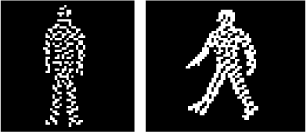
\includegraphics[width=0.75\textwidth]{images/00127.png}
  \caption{混合虚拟宠物游戏原型}
  \label{fig:mixed_pet_prototype}
\end{figure}

\begin{exercise}{统一宠物世界 VAnimal}{106}
定义分类数据 \code{VAnimal}：
\begin{lstlisting}[language=BSL]
; 一个 VAnimal 是以下两者之一：
; -- VCat
; -- VCham
\end{lstlisting}
设计世界程序，在画布上渲染当前激活的宠物，并处理其饥饿流逝与按键抚摸互动。
\end{exercise}

\begin{exercise}{猫与变色龙双宠乐园}{107}
设计一个同时容纳小猫和变色龙的双宠世界程序 \code{cham-and-cat}。定义一个包含两个宠物的结构体，让它们在同一张画布上并排漫步。
\end{exercise}

\begin{exercise}{行人过街信号灯倒计时}{108}
设计一个逼真的行人过街交通灯：
\begin{itemize}
  \item 默认状态：红色背景，站立的橙色小人；
  \item 收到通行信号：切换为绿色背景，行走的绿色小人，持续 10 秒；
  \item 随后进入数字倒计时：显示数字 $9, 8, \dots, 0$。奇数显示为橙色，偶数显示为绿色；
  \item 倒计时归零后切回默认禁行状态。
\end{itemize}
\end{exercise}

\begin{exercise}{按键序列模式识别机}{109}
设计一个识别特定按键序列的世界程序：初始显示 $100 \times 100$ 的白色方块；当用户按下首个目标字符时变为黄色；输入完最终字符后变为绿色；若在任何步骤输入错误按键，则方块立即变红报警。
\end{exercise}

% ==============================================================================
\section{输入错误与防御性设计}
\label{sec:6.3_input_errors}
% ==============================================================================

在此前的所有函数设计中，我们默认函数的调用者都是“守规矩”的合作者——传递的实参类型完全符合函数签名。但在真实生产环境中，函数随时可能遭遇非法实参的恶意或误操作调用。

如果一个计算圆面积的函数被传递了字符串 \code{"five"} 或负数 $-10$：
\begin{lstlisting}[language=BSL]
(define (area-of-disk r)
  (* 3.14 (sqr r)))
\end{lstlisting}
传递 \code{"five"} 会引发底层原始算术操作符的崩溃，而传递 $-10$ 甚至会静默地输出一个看似合理但物理错误的答案！

BSL 提供了 \code{error} 函数用于显式抛出运行时错误，并提供了 \code{check-error} 用于对错误处理进行单元测试：

\begin{lstlisting}[language=BSL]
; Any -> Number
; 带防御性参数校验的圆盘面积计算函数
(check-expect (checked-area-of-disk 2) (* 3.14 4))
(check-error (checked-area-of-disk "two") "area-of-disk: number expected")
(check-error (checked-area-of-disk -3) "area-of-disk: positive number expected")

(define (checked-area-of-disk v)
  (cond
    [(and (number? v) (>= v 0)) (area-of-disk v)]
    [(not (number? v)) (error "area-of-disk" "number expected")]
    [else (error "area-of-disk" "positive number expected")]))
\end{lstlisting}

\begin{exercise}{校验正数面积输入}{110}
完整实现并测试 \code{checked-area-of-disk}，确保其在输入合法正数、零、负数以及非数值类型时均给出精确的行为。
\end{exercise}

\begin{exercise}{防御性二维向量构造}{111}
考虑结构体 \code{(define-struct vec [x y])}。设计函数 \code{checked-make-vec}，校验两个坐标分量必须均为正数，否则抛出详尽的错误提示。
\end{exercise}

% ==============================================================================
\section{检查世界状态}
\label{sec:6.4_checking_the_world}
% ==============================================================================

在调试复杂的世界程序时，程序崩溃常常发生在某个深层子函数中，但真正的罪魁祸首却是上一轮时钟滴答生成的非法世界状态。

为了捍卫系统边界，我们应当为每一个自定义数据定义编写\term{类型识别谓词}（Type Predicates）：

\begin{lstlisting}[language=BSL]
; Any -> Boolean
; 判定给定值是否为一个合法的导弹发射阶段状态
(define (fired-state? v)
  (and (fired? v)
       (posn? (fired-ufo v))
       (tank? (fired-tank v))
       (posn? (fired-missile v))))
\end{lstlisting}

\begin{exercise}{使用 or 重构谓词}{112}
使用 \code{or} 表达式重构复合类型判定函数，使其逻辑更加精炼。
\end{exercise}

\begin{exercise}{为核心数据定义编写谓词}{113}
分别为前文中的 \code{SIGS}、\code{Coordinate} 以及 \code{VAnimal} 设计完整的类型验证谓词。
\end{exercise}

\begin{exercise}{全面装备世界程序}{114}
使用练习~\ref{ex:113} 中编写的谓词，为太空侵略者、虚拟宠物以及文本编辑器世界程序装配状态自检断言。
\end{exercise}

% ==============================================================================
\section{相等性谓词}
\label{sec:6.5_equality_predicates}
% ==============================================================================

BSL 为基本类型提供了各自的相等性比较函数：\code{=} 用于比较数，\code{string=?} 用于比较字符串，\code{boolean=?} 用于比较布尔值。但对于程序员自定义的枚举与结构体，BSL 并没有提供开箱即用的比对函数。

考虑第 4.7 节中的交通信号灯枚举 \code{TrafficLight}。要判断两个交通信号灯状态是否完全一致，我们应当遵循设计配方编写专属的相等性谓词：

\begin{lstlisting}[language=BSL]
; TrafficLight TrafficLight -> Boolean
; 判断两盏交通信号灯的状态是否相同
(check-expect (light=? "red" "red") #true)
(check-expect (light=? "red" "green") #false)
(check-expect (light=? "green" "green") #true)
(check-expect (light=? "yellow" "yellow") #true)

(define (light=? a-light another-light)
  (string=? a-light another-light))
\end{lstlisting}

如果我们希望进一步增强该函数的鲁棒性，让它在接收到非信号灯字符串时主动报错，便可以借助前文的错误校验机制：

\begin{exercise}{智能报错的信号灯比较谓词}{115}
修改 \code{light=?} 函数，使其在遇到非法输入时不仅抛出错误，还能在错误消息中明确指出究竟是第几个实参不是合法的 \code{TrafficLight}。
\end{exercise}

% ==============================================================================
% 第 7 章：第一部分小结 (Chapter 7: Summary)
% ==============================================================================

\chapter{第一部分小结}
\label{sec:ch07_summary}

在本书的第一部分中，你学习了一系列看似质朴却至关重要的编程铁律。作为本阶段的收束，我们将其精要归纳如下：

\begin{notebox}[第一部分核心心得归纳]
\begin{enumerate}[label=\textbf{\arabic*.}]
  \item \textbf{设计胜于修补}：
    优秀的程序员\term{系统性地设计}程序；拙劣的程序员则盲目拼凑代码，不断打补丁，直到程序“表面上似乎能跑起来”为止。编程不是试错的撞大运，而是严密的工程思维。

  \item \textbf{设计配方的两个维度}：
    程序设计配方具有紧密交织的两个维度：
    \begin{itemize}
      \item \textbf{过程维度}：即开发必须遵循的严谨步骤序列——从数据定义、函数签名、目的说明与函数头，到设计功能测试、梳理模板、编写函数体，最终运行自动化测试。
      \item \textbf{数据维度}：即所选取的\textbf{数据表示形态}（原子类型、枚举、区间、分类、结构体）如何直接决定了函数模板的骨架与实现方式。
    \end{itemize}

  \item \textbf{良构程序的解剖结构}：
    每一个精心设计的程序都由多项常量定义、结构体类型定义、数据定义以及函数定义有机协同构成：
    \begin{itemize}
      \item \textbf{批处理程序}（Batch Programs）：由一个 \code{main} 主函数统领全局，该主函数通常组合若干专职辅助函数来完成复杂的端到端计算。
      \item \textbf{交互式程序}（Interactive Programs）：由 \code{big-bang} 表达式承担主函数的职责；它规定了世界的初始状态、一个生成画面的渲染函数，以及至多三个核心事件处理器（时钟滴答处理、鼠标点击处理、键盘事件处理）。
      \item 无论是哪种程序，函数定义在源文件中均应以\textbf{自顶向下}（top-down）的方式布局：首先呈现主函数，接着呈现主函数直接调用的下层函数，依此类推。
    \end{itemize}

  \item \textbf{语法与计算语义}：
    与一切自然语言和程序设计语言相同，初学学生语言（BSL）拥有一套严密的词汇与文法规则。程序员必须深刻理解语言中每一条合法语句的\term{计算含义}（语义），从而能够准确预测程序在接收特定输入时将如何一步步归约求值。接下来的插曲将深入剖析这一概念。

  \item \textbf{拥抱标准库，避免重复造轮子}：
    包括 BSL 在内的现代编程语言都提供了丰富的标准库函数（例如图形库 \code{2htdp/image} 与宇宙模拟库 \code{2htdp/universe}）。优秀程序员应当熟练掌握标准库提供的武器，尤其是其函数签名与目的说明，善用现成的高效工具解决问题。

  \item \textbf{熟练驾驭语言工具与术语}：
    程序员必须对自己所选编程语言提供的各类机制了如指掌。这些机制要么是语言的核心构件（如 \code{cond} 或 \code{max}），要么是从库中导入的利器。在此精神下，请读者务必确保自己已经毫无障碍地彻底掌握以下核心概念：
    \begin{itemize}
      \item 结构体类型定义（Structure Type Definition）
      \item 函数定义（Function Definition）
      \item 常量定义（Constant Definition）
      \item 结构体实例（Structure Instance）
      \item 数据定义与解释（Data Definition and Interpretation）
      \item 世界主控表达式 \code{big-bang}
      \item 事件处理函数（Event-Handling Function）
    \end{itemize}
\end{enumerate}
\end{notebox}

% ==============================================================================
% 插曲 1：初学学生语言 (Intermezzo 1: Beginning Student Language)
% ==============================================================================

\intermezzo{插曲 1：初学学生语言 (BSL)}
\label{sec:intermezzo01}

在本书的第一部分中，我们通过直观的示例与非正式的说明学习了初学学生语言（BSL）。现在是时候停下匆忙的脚步，系统性地审视这门小巧却极其严谨的编程语言的全貌了。

一门程序设计语言由两个核心部分构成：
\begin{itemize}
  \item \term{句法}（Syntax）：规定了哪些符号序列构成合法的程序句子（包括词汇与文法）；
  \item \term{语义}（Semantics）：精确阐明了合法的程序句子在计算机内部如何一步步执行归约（计算含义）。
\end{itemize}

本插曲将带你全面梳理 BSL 的词汇表、核心文法、等量代换计算模型、短路布尔求值、结构体运行机制以及详尽的常见错误诊断手册。

% ==============================================================================
\intermezzosection{BSL 词汇 (BSL Vocabulary)}
\label{sec:int01_vocabulary}
% ==============================================================================

在任何语言中，基本词汇被称为\term{词素}或\term{词法记号}（Tokens）。BSL 的核心词汇包含四类：
\begin{enumerate}
  \item \textbf{字面常量}（Literal Constants）：数（如 \code{42}, \code{3.14}, \code{-5/9}）、布尔值（\code{\#true}, \code{\#false}）、字符串（如 \code{"hello"}）以及图像；
  \item \textbf{标识符}（Identifiers / Names）：变量名、函数名与字段名。BSL 对标识符的命名极其宽容，几乎允许任何不包含空格和圆括号的字符序列（例如 \code{string->number}, \code{distance-to-0}, \code{traffic-light?} 等）；
  \item \textbf{关键字}（Keywords）：具有特殊语法地位的保留字，如 \code{define}, \code{define-struct}, \code{cond}, \code{else}, \code{check-expect} 等；
  \item \textbf{标点符号}：开闭圆括号 \code{(} 与 \code{)}，以及等价的开闭方括号 \code{[} 与 \code{]}。
\end{enumerate}

\begin{figure}[htbp]
  \centering
  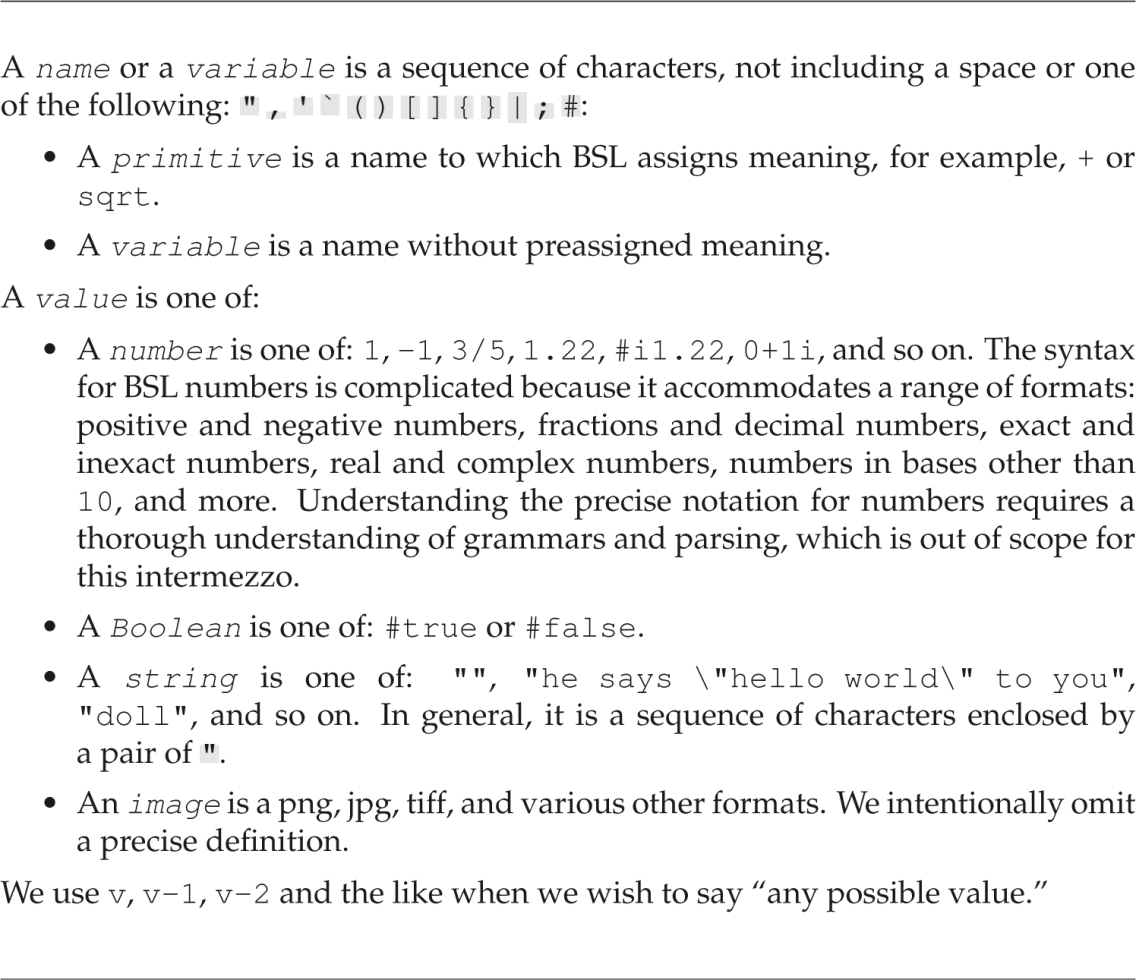
\includegraphics[width=0.85\textwidth]{images/00134.png}
  \caption{BSL 核心词汇体系}
  \label{fig:bsl_vocab}
\end{figure}

% ==============================================================================
\intermezzosection{BSL 文法 (BSL Grammar)}
\label{sec:int01_grammar}
% ==============================================================================

文法规定了如何将词汇组合为合法的表达式与定义。计算机科学家使用一种称为“上下文无关文法”（Context-Free Grammar）的代数表示法来定义语言规则。

\begin{figure}[htbp]
  \centering
  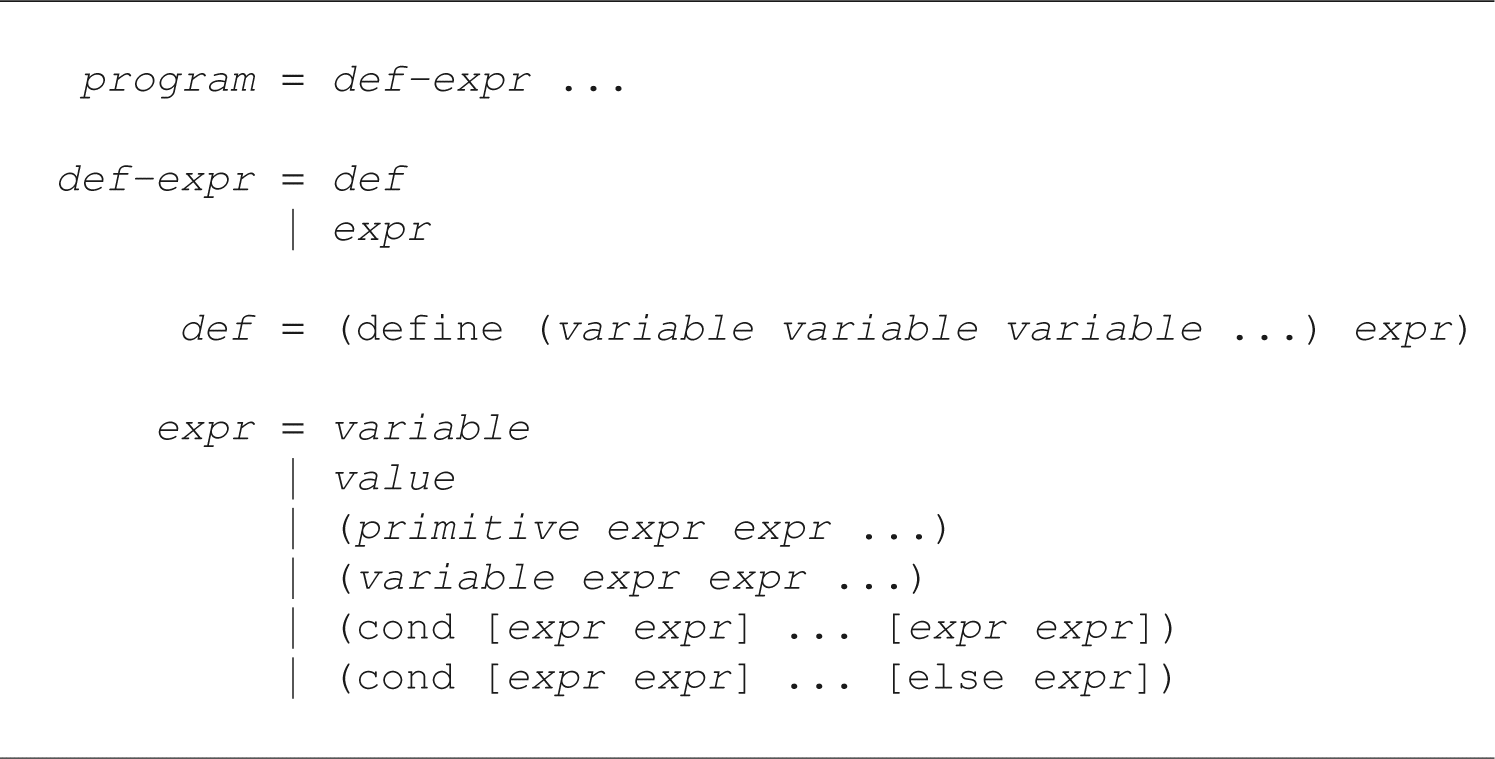
\includegraphics[width=0.85\textwidth]{images/00135.png}
  \caption{BSL 核心表达式与定义文法}
  \label{fig:bsl_grammar}
\end{figure}

图~\ref{fig:bsl_grammar} 展示了 BSL 的核心文法法则：
\begin{itemize}
  \item 一个\term{程序}（Program）是由零个或多个定义和表达式构成的序列；
  \item 一个\term{定义}（Definition）具有以下形式之一：
    \begin{itemize}
      \item 常量定义：\code{(define } Variable \code{ } Expression\code{)}
      \item 函数定义：\code{(define (} FunctionName Variable $\dots$ Variable\code{) } Expression\code{)}
      \item 结构体类型定义：\code{(define-struct } StructureName \code{[} FieldName $\dots$ FieldName\code{])}
    \end{itemize}
  \item 一个\term{表达式}（Expression）可以是值、变量、函数应用、条件表达式或逻辑运算。
\end{itemize}

\begin{figure}[htbp]
  \centering
  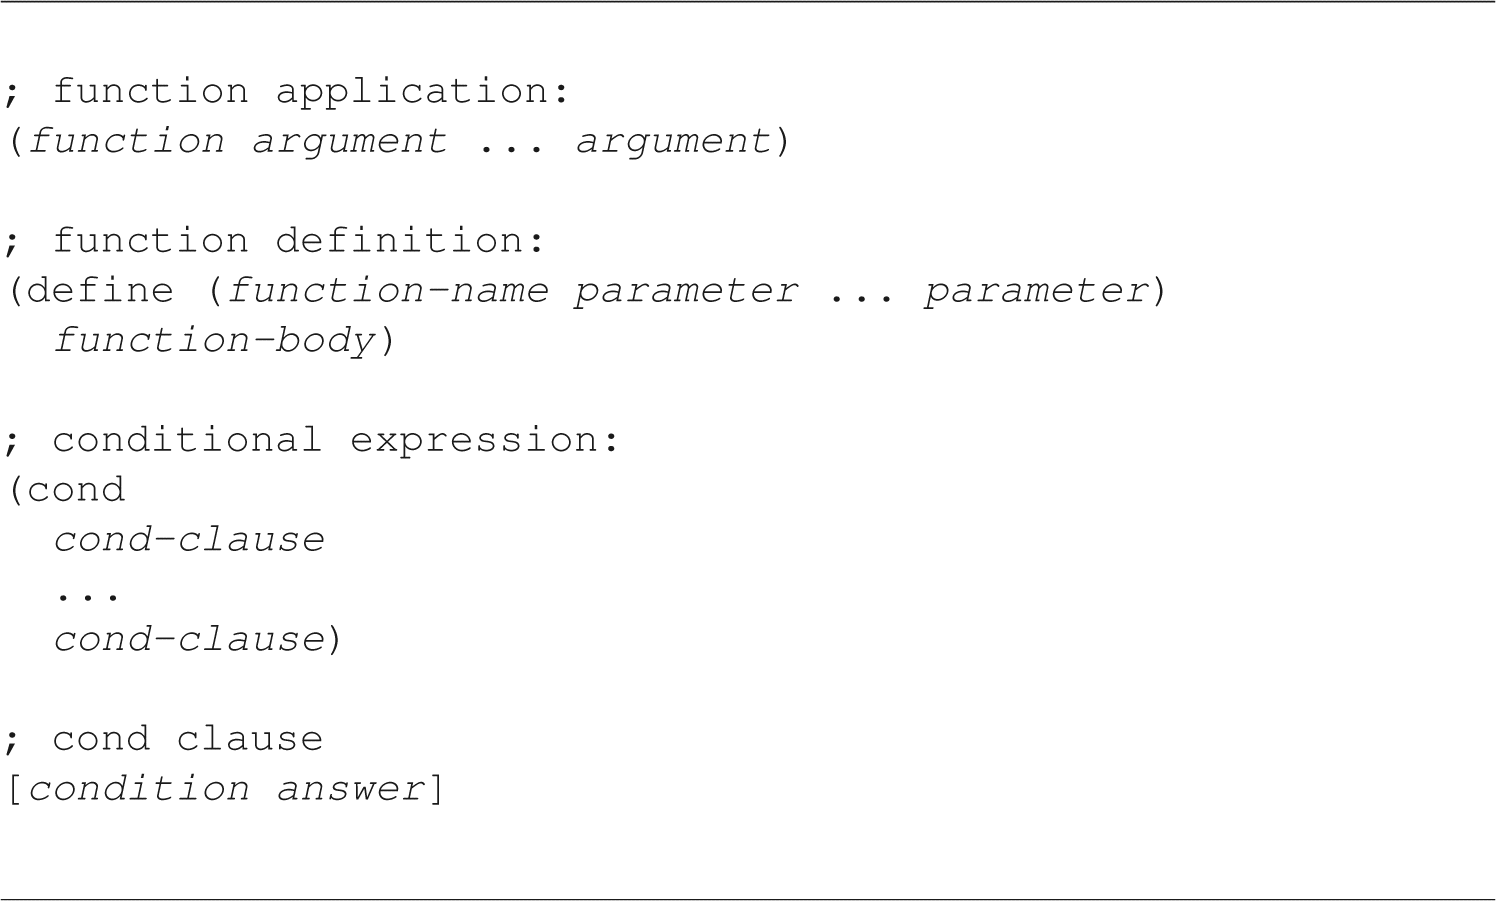
\includegraphics[width=0.75\textwidth]{images/00136.png}
  \caption{BSL 句法命名规范与元变量说明}
  \label{fig:bsl_naming_conventions}
\end{figure}

\begin{exercise}{文法合法性辨析 1}{116}
根据图~\ref{fig:bsl_grammar} 的文法规则，判断以下句子是否为合法的 BSL 表达式：
\begin{lstlisting}[language=BSL]
x
(= x 5)
(= (= x 5) 0)
\end{lstlisting}
\end{exercise}

\begin{exercise}{文法合法性辨析 2}{117}
判断以下语句是否为合法的 BSL 定义或表达式：
\begin{lstlisting}[language=BSL]
(3 + 4)
number?
(x)
\end{lstlisting}
\end{exercise}

\begin{exercise}{文法合法性辨析 3}{118}
仔细观察以下句子，解释为什么它们是合法或非法的：
\begin{lstlisting}[language=BSL]
(define (f x) x)
(define (f x) y)
(define (f x y) 3)
\end{lstlisting}
\end{exercise}

\begin{exercise}{文法合法性辨析 4}{119}
判断以下句子是否符合 BSL 文法：
\begin{lstlisting}[language=BSL]
(define (f) 10)
(define (f x y z) (x))
(define (f) (cond [(> 1 0) 10] [else 20]))
\end{lstlisting}
\end{exercise}

\begin{exercise}{综合文法甄别}{120}
区分以下句子中哪些是合法的 BSL 结构，哪些是非法的：
\begin{lstlisting}[language=BSL]
(+ 1 (not x))
(+ 1 2 3)
(cond)
(cond [else 10])
(cond [(< x 0) 10] [else 20])
\end{lstlisting}
\end{exercise}

% ==============================================================================
\intermezzosection{BSL 语义 (BSL Meaning)}
\label{sec:int01_meaning}
% ==============================================================================

如果一个程序在文法上是合法的，它就拥有了明确的\term{计算语义}。BSL 的最迷人之处在于：\textbf{它的语义完全可以用初等代数中的“等量代换”（Replacing Equals by Equals）来解释！}

\begin{figure}[htbp]
  \centering
  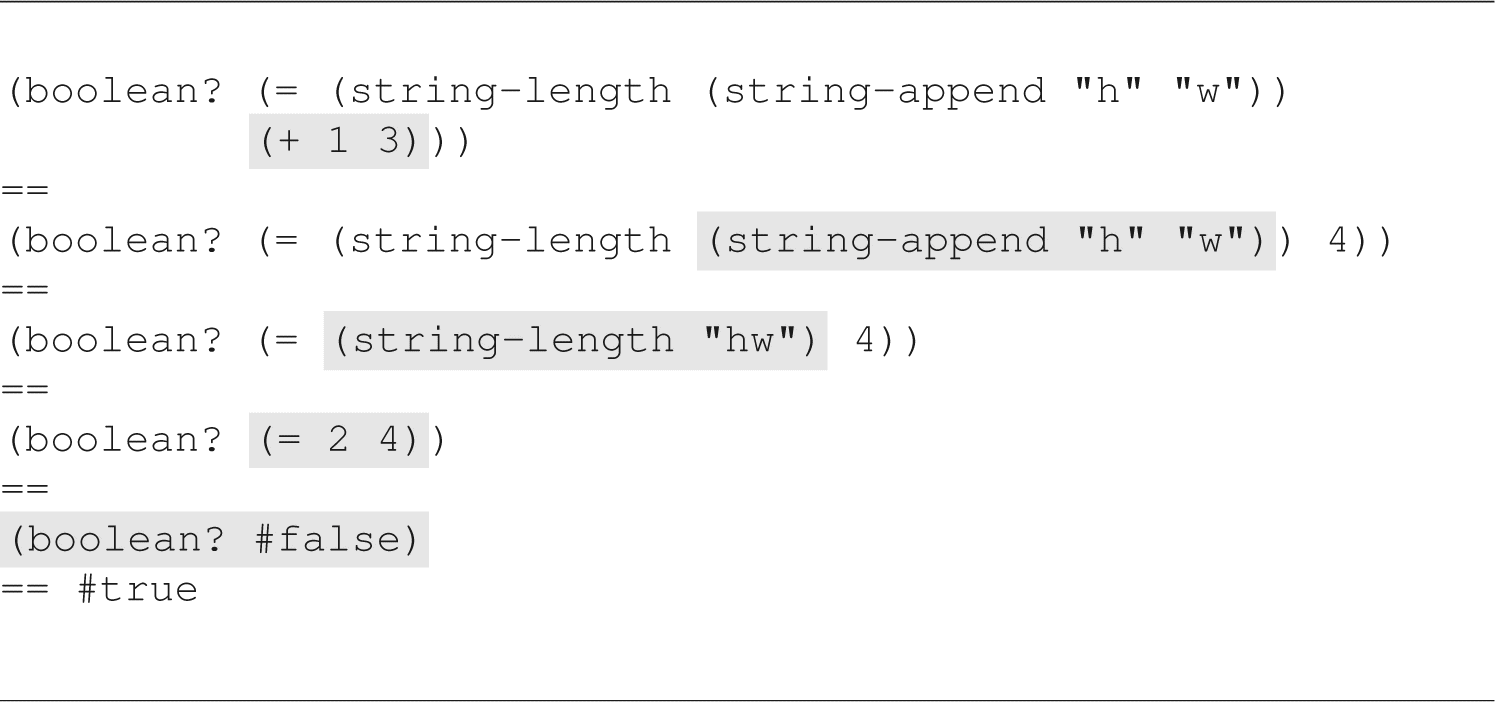
\includegraphics[width=0.85\textwidth]{images/00138.png}
  \caption{基于等量代换的算术归约示例}
  \label{fig:equals_by_equals}
\end{figure}

当对函数应用 \code{(f } $v_1 \dots v_n$\code{)} 求值时，只要所有实参 $v_i$ 都已经被计算为具体的值（Value），归约机制就会找到函数 \code{f} 的定义：
\begin{lstlisting}[language=BSL]
(define (f x_1 ... x_n) BodyExpression)
\end{lstlisting}
并将整个函数调用替换为 \code{BodyExpression}，其中所有的形参 $x_i$ 都被相应的实参值 $v_i$ 所替换！

\begin{exercise}{表达式单步归约推导}{121}
单步手工推演以下表达式的求值全过程：
\begin{lstlisting}[language=BSL]
(+ (* (/ 12 8) 2/3) (- 10 (sqrt 4)))
(cond [(= 0 0) #false] [(> 2 1) (string=? "a" "b")] [else (= 0 2)])
(cond [(= 2 0) #false] [(> 2 1) (string=? "a" "a")] [else (= 0 2)])
\end{lstlisting}
\end{exercise}

\begin{exercise}{函数调用单步推导}{122}
假设定义区包含以下定义：
\begin{lstlisting}[language=BSL]
(define (f x y)
  (+ (* 3 x) (* (+ y 1) 4)))
\end{lstlisting}
单步推演以下调用的计算过程：
\begin{lstlisting}[language=BSL]
(+ (f 1 2) (f 2 1))
(f 1 (* 2 3))
(f (f 1 (* 2 3)) 19)
\end{lstlisting}
\end{exercise}

% ==============================================================================
\intermezzosection{语义与计算 (Meaning and Computing)}
\label{sec:int01_computing}
% ==============================================================================

在 DrRacket 中，你无需仅凭纸笔进行上述推演。DrRacket 内置了世界一流的教学工具——\term{单步执行器}（The Stepper）。点击工具栏上的“Step”按钮，单步执行器将以绿色高亮当前正在被求值的子表达式（Redex），并以紫色高亮其代换后的结果。

每当你对某个复杂函数在特定输入下的执行路径感到困惑时，单步执行器就是你最权威、最直观的导师。

% ==============================================================================
\intermezzosection{BSL 错误 (BSL Errors)}
\label{sec:int01_errors}
% ==============================================================================

在编程中，错误主要分为两大范畴：
\begin{enumerate}
  \item \textbf{句法错误}（Syntax Errors）：代码不符合文法规则，程序根本无法被解析或启动；
  \item \textbf{运行时错误}（Runtime Errors）：代码符合文法，但在执行过程中遭遇了非法的算术或类型操作（如除以零、将数传递给需要字符串的函数等）。
\end{enumerate}

% ==============================================================================
\intermezzosection{布尔表达式 (Boolean Expressions)}
\label{sec:int01_boolean_expressions}
% ==============================================================================

逻辑运算 \code{and} 与 \code{or} 在 BSL 中具有特殊的“短路求值”（Short-Circuit Evaluation）语义：
\begin{itemize}
  \item \code{(and exp\_1 exp\_2 ...)}：从左到右求值。一旦某个表达式求得 \code{\#false}，整个 \code{and} 立即返回 \code{\#false}，后续表达式根本不会被计算！
  \item \code{(or exp\_1 exp\_2 ...)}：从左到右求值。一旦某个表达式求得 \code{\#true}，整个 \code{or} 立即返回 \code{\#true}，后续表达式被直接跳过。
\end{itemize}

事实上，\code{and} 与 \code{or} 本质上是 \code{cond} 表达式的语法糖：
\begin{align*}
\code{(and $e\_1$ $e\_2$)} &\equiv \code{(cond [$e\_1$ $e\_2$] [else \#false])} \\
\code{(or $e\_1$ $e\_2$)}  &\equiv \code{(cond [$e\_1$ \#true] [else $e\_2$])}
\end{align*}

\begin{exercise}{用 cond 重写 if 与 and}{123}
写出形式化规则，说明如何将任何形如 \code{(if condition then-exp else-exp)} 的表达式重构为等价的 \code{cond} 表达式。
\end{exercise}

% ==============================================================================
\intermezzosection{常量定义 (Constant Definitions)}
\label{sec:int01_constant_definitions}
% ==============================================================================

定义区的常量定义是自顶向下依次被求值的。一旦一个常量被绑定到值上，在该定义之后的任何地方都可以引用这个名字。

\begin{exercise}{常量定义的推导}{124}
单步推演以下程序的执行顺序，解释常量绑定与函数定义的依赖关系：
\begin{lstlisting}[language=BSL]
(define PRICE 5)
(define SALES-TAX (* 0.08 PRICE))
(define TOTAL (+ PRICE SALES-TAX))
\end{lstlisting}
\end{exercise}

% ==============================================================================
\intermezzosection{结构体类型定义 (Structure Type Definitions)}
\label{sec:int01_structure_type_definitions}
% ==============================================================================

结构体类型定义向语言中添加了构造函数、选择器与谓词。

特别需要明确：\textbf{结构体实例本身就是一种一等公民的“值”（Value）}。
例如，\code{(make-posn 3 4)} 是一个值；但 \code{(make-posn (+ 1 2) 4)} 并不是值，而是一个尚未完全求值的表达式，它需要先将各参数归约为值，才能生成最终的结构体实例。

\begin{exercise}{区分合法句子}{125}
甄别以下结构体相关语句的文法合法性：
\begin{lstlisting}[language=BSL]
(define-struct oops [])
(define-struct child [parents dob date])
(define-struct (child person) [dob extra])
\end{lstlisting}
\end{exercise}

\begin{exercise}{辨识结构体值}{126}
假设定义区包含 \code{(define-struct point [x y])}。在以下各项中，哪些已经是最终的“值”，哪些是仍需计算的表达式？
\begin{lstlisting}[language=BSL]
(make-point 1 2)
(make-point (make-point 1 2) 3)
(make-point (+ 1 2) 3)
\end{lstlisting}
\end{exercise}

\begin{exercise}{结构体字段提取推导}{127}
单步推导以下包含结构体选择器的复杂表达式：
\begin{lstlisting}[language=BSL]
(define-struct ball [x y deltax deltay])
(number? (ball-x (make-ball 1 2 3 4)))
(ball-deltax (make-ball 1 2 3 4))
\end{lstlisting}
\end{exercise}

% ==============================================================================
\intermezzosection{BSL 测试 (BSL Tests)}
\label{sec:int01_bsl_tests}
% ==============================================================================

测试是程序设计中不可或缺的基石。图~\ref{fig:bsl_full_grammar} 呈现了包含了完整测试机制的 BSL 终极文法。

\begin{figure}[htbp]
  \centering
  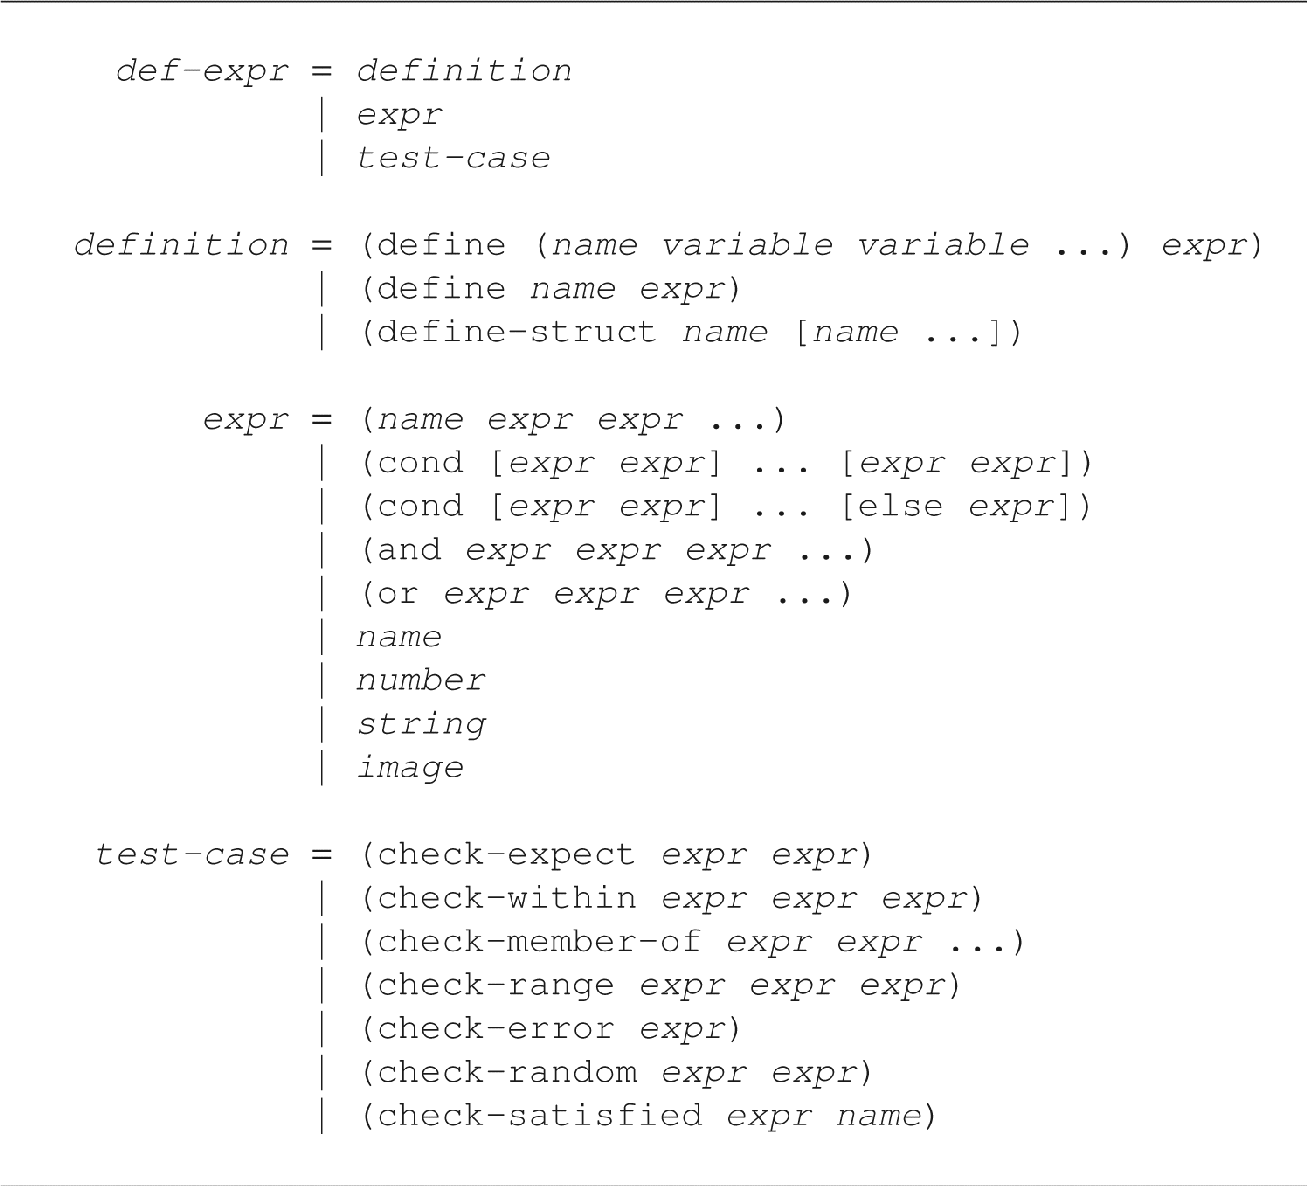
\includegraphics[width=0.85\textwidth]{images/00141.png}
  \caption{BSL 完整语法规范（包含测试套件）}
  \label{fig:bsl_full_grammar}
\end{figure}

BSL 提供了三种核心测试断言：
\begin{itemize}
  \item \code{(check-expect Expression\_1 Expression\_2)}：断言两个表达式产生严格完全相同的值；
  \item \code{(check-within Expression\_1 Expression\_2 Tolerance)}：用于浮点数或不精确数的近似比较（误差在 \code{Tolerance} 范围内）；
  \item \code{(check-error Expression ExpectedErrorMessage)}：断言前一个表达式必定抛出带有指定提示文本的运行时错误。
\end{itemize}

\begin{exercise}{运行单元测试套件}{128}
将以下测试复制到 DrRacket 定义区并运行，观察测试报告窗口的反馈：
\begin{lstlisting}[language=BSL]
(check-expect 3 3)
(check-member-of "green" "red" "yellow" "green")
(check-within (sqrt 2) 1.414 0.001)
(check-range 5 0 10)
(check-error (/ 1 0) "/: division by zero")
\end{lstlisting}
\end{exercise}

% ==============================================================================
\intermezzosection{BSL 错误信息详查 (BSL Error Messages)}
\label{sec:int01_error_messages}
% ==============================================================================

面对错误提示时的沉着与从容，是新手迈向专业程序员的重要标志。下文汇总了初学者在 BSL 中最常遭遇的典型错误场景。

\subsection{函数应用相关错误}

假设定义区仅有 \code{(define (average x y) (/ (+ x y) 2))}。

\begin{figure}[htbp]
  \centering
  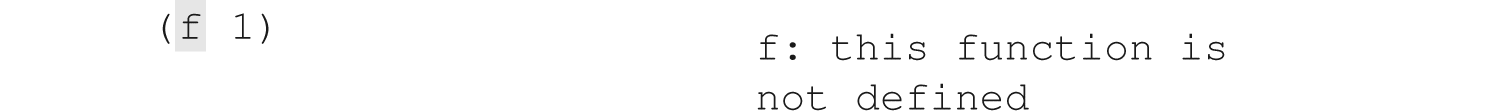
\includegraphics[width=0.75\textwidth]{images/00145.png}
  \caption{未定义函数错误：调用了不存在的函数名}
  \label{fig:err_undefined_fn}
\end{figure}

\begin{figure}[htbp]
  \centering
  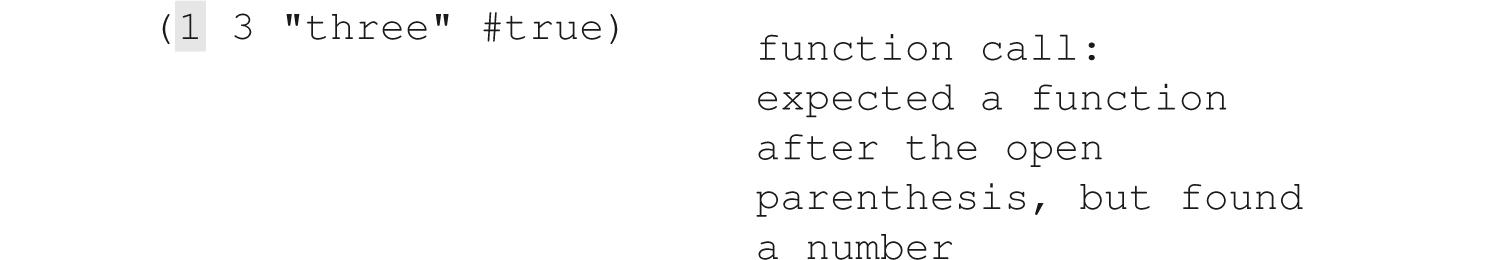
\includegraphics[width=0.75\textwidth]{images/00146.png}
  \caption{括号后缺少函数名：开括号后紧跟了数值而不是操作符}
  \label{fig:err_expected_fn}
\end{figure}

\begin{figure}[htbp]
  \centering
  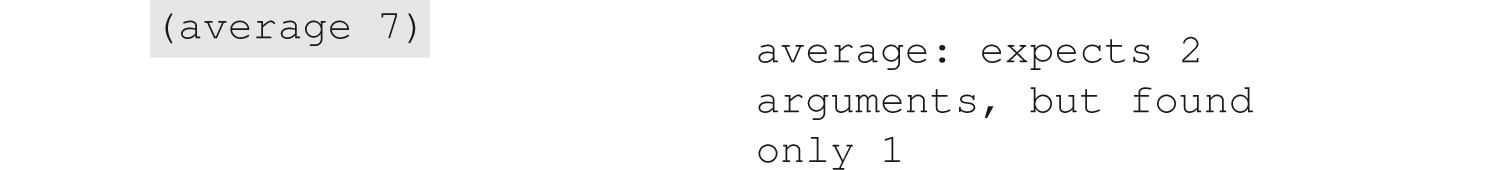
\includegraphics[width=0.75\textwidth]{images/00147.png}\\[1ex]
  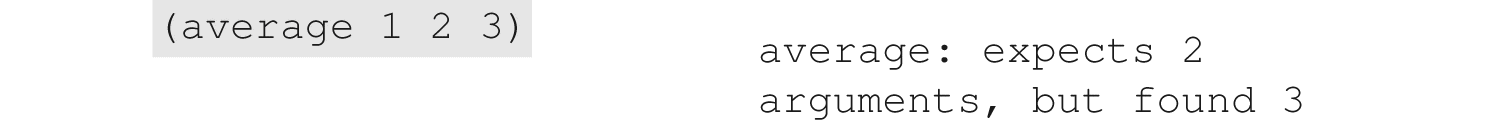
\includegraphics[width=0.75\textwidth]{images/00148.png}
  \caption{实参个数不匹配：传入参数过少（上）或过多（下）}
  \label{fig:err_arg_mismatch}
\end{figure}

\subsection{数据类型不匹配错误}

\begin{figure}[htbp]
  \centering
  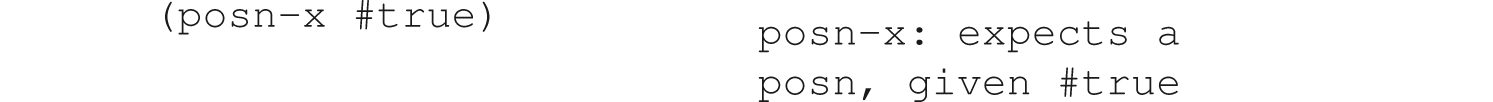
\includegraphics[width=0.75\textwidth]{images/00150.png}\\[1ex]
  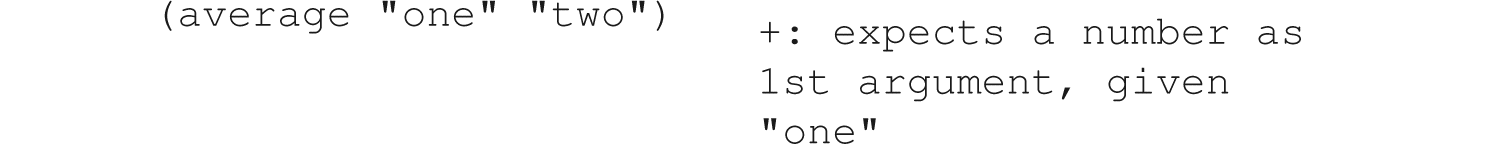
\includegraphics[width=0.75\textwidth]{images/00151.png}
  \caption{类型契约违背：向选择器或算术操作符传递了错误类型的值}
  \label{fig:err_type_contract}
\end{figure}

如图~\ref{fig:err_type_contract} 所示，\code{posn-x} 期望接收一个 \code{posn} 结构体，却收到了整数 73；算术加法 \code{+} 期望接收数值，却收到了字符串 \code{"hello"}。

\subsection{条件表达式与定义相关错误}

\begin{figure}[htbp]
  \centering
  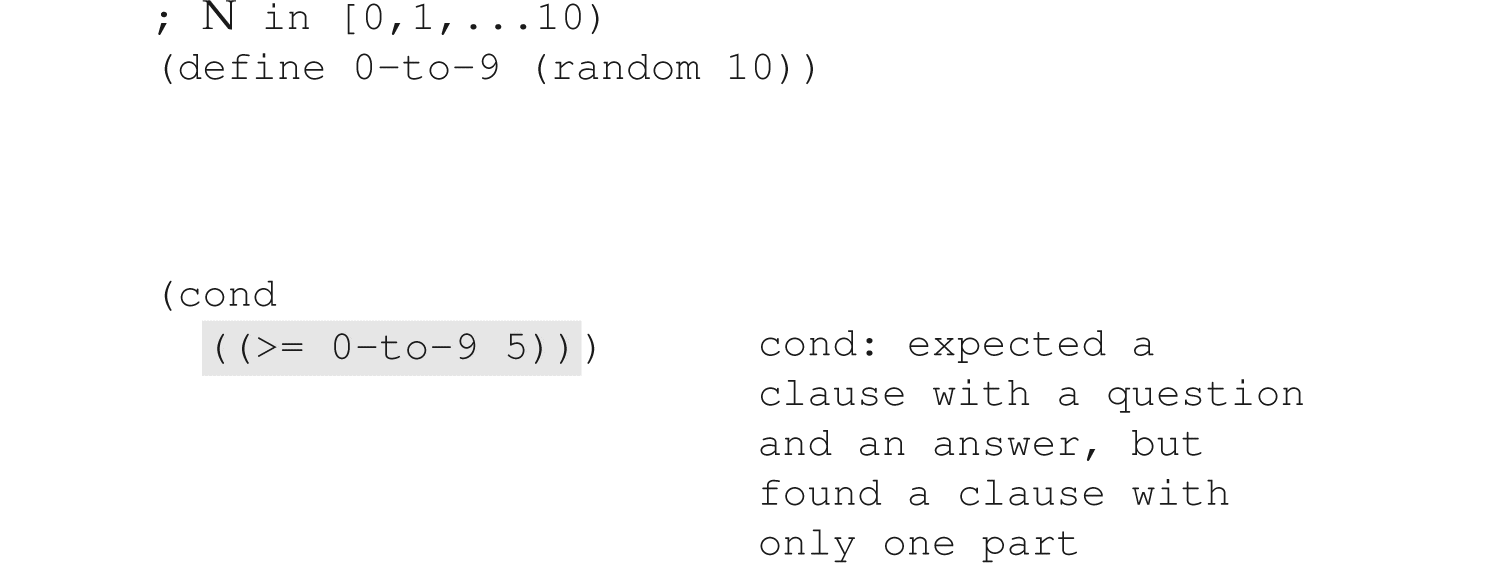
\includegraphics[width=0.75\textwidth]{images/00152.png}\\[1ex]
  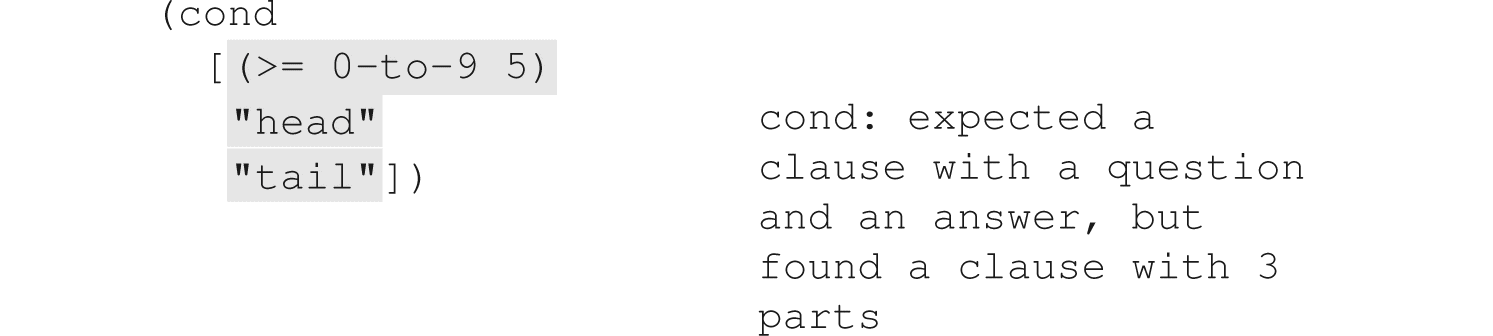
\includegraphics[width=0.75\textwidth]{images/00153.png}
  \caption{cond 分支格式错误}
  \label{fig:err_cond_shape}
\end{figure}

\begin{figure}[htbp]
  \centering
  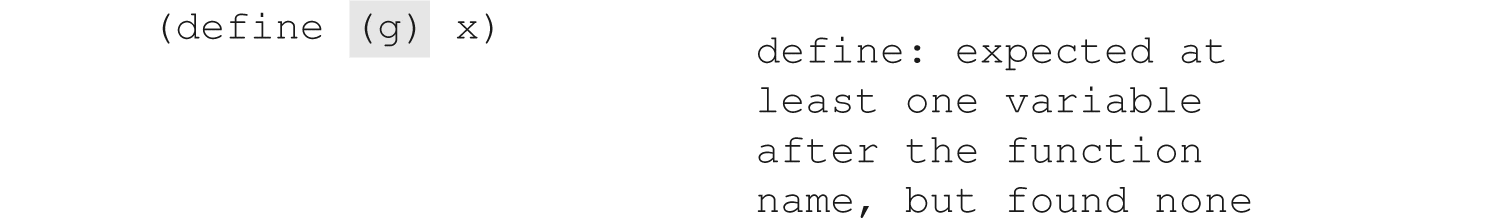
\includegraphics[width=0.75\textwidth]{images/00157.png}\\[1ex]
  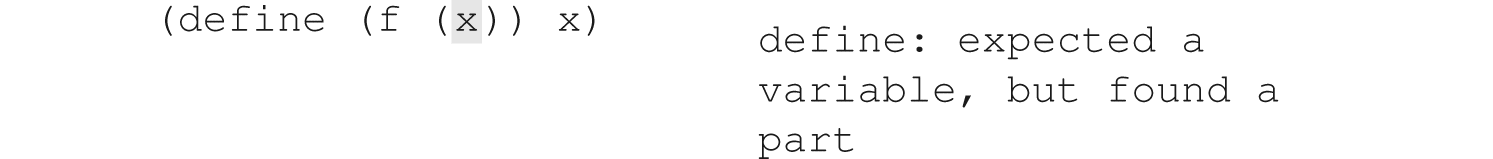
\includegraphics[width=0.75\textwidth]{images/00158.png}
  \caption{函数头缺少参数或语法格式错误}
  \label{fig:err_redefinition}
\end{figure}

当你在编写代码遭遇错误时，请沉着阅读高亮提示并对照上述图集，追溯文法与类型规范，你将能够迅速定位根因并优雅修正！


% ==================== 第二部分：任意大小的数据 ====================
\part{任意大小的数据 (Arbitrarily Large Data)}
% ==============================================================================
% 第 8 章：列表 (Chapter 8: Lists)
% ==============================================================================

\chapter{列表}
\label{sec:ch08_lists}

你在此前很可能从未接触过\term{自引用定义}（self-referential definition）。你的语文老师肯定会对这类定义敬而远之，而许多数学课程在涉及这类定义时往往语焉不详。然而，程序员绝不能含糊其辞，他们的工作要求绝对的精确性。虽然一般而言一个定义可能包含多处对自身的引用，但本章将从最有用的例子——列表（list）开始，展示仅需一次自引用的优雅范例。

引入列表还极大地丰富了我们所能研究的应用类型。本章将通过丰富的实例精心建立你的直觉，同时为下一章修订程序设计配方提供充足的动机——下一章将系统阐述如何针对自引用数据定义编写函数。

\section{创建列表}
\label{sec:ch08_creating_lists}

我们每个人在日常生活中都在不停地列清单。在去超市购物前，我们会写下一张采购清单；有些人每天早晨都会列一份待办事项（to-do list）；在十二月，许多孩子会准备一份圣诞愿望清单；为了筹办聚会，我们会整理一份邀请宾客的名单。将信息组织成列表形式，早已融入我们生活的方方面面。

既然信息天然呈现为列表的形式，我们就必须学会如何在 BSL 中将此类列表表示为数据。事实上，正因为列表至关重要，BSL 像支持笛卡尔坐标点（\code{posn}）一样，内置了对创建和操作列表的原生支持。但与坐标点不同的是，列表的数据定义永远由你自己来决定。不过我们先从最基础的开始：创建列表。

当构建一个列表时，我们总是从\term{空列表}（empty list）开始。在 BSL 中，空列表表示为：
\begin{lstlisting}[language=BSL]
'()
\end{lstlisting}
读作“empty”，即“空列表”的简写。与 \code{\#true} 或 \code{5} 一样，\code{'()} 也是一个常量。当我们向列表中添加元素时，就会构造出一个新的列表；在 BSL 中，\code{cons} 操作正是用于此目的。例如：
\begin{lstlisting}[language=BSL]
(cons "Mercury" '())
\end{lstlisting}
它由空列表 \code{'()} 和字符串 \code{"Mercury"} 构造出一个包含一个元素的列表。图~\ref{fig:building_a_list} 以我们之前展示结构体相同的图示方法展示了这个列表。\code{cons} 方框有两个字段：\code{first}（首元素）和 \code{rest}（其余部分）。在此例中，\code{first} 字段存放 \code{"Mercury"}，而 \code{rest} 字段存放 \code{'()}。

\begin{figure}[htbp]
  \centering
  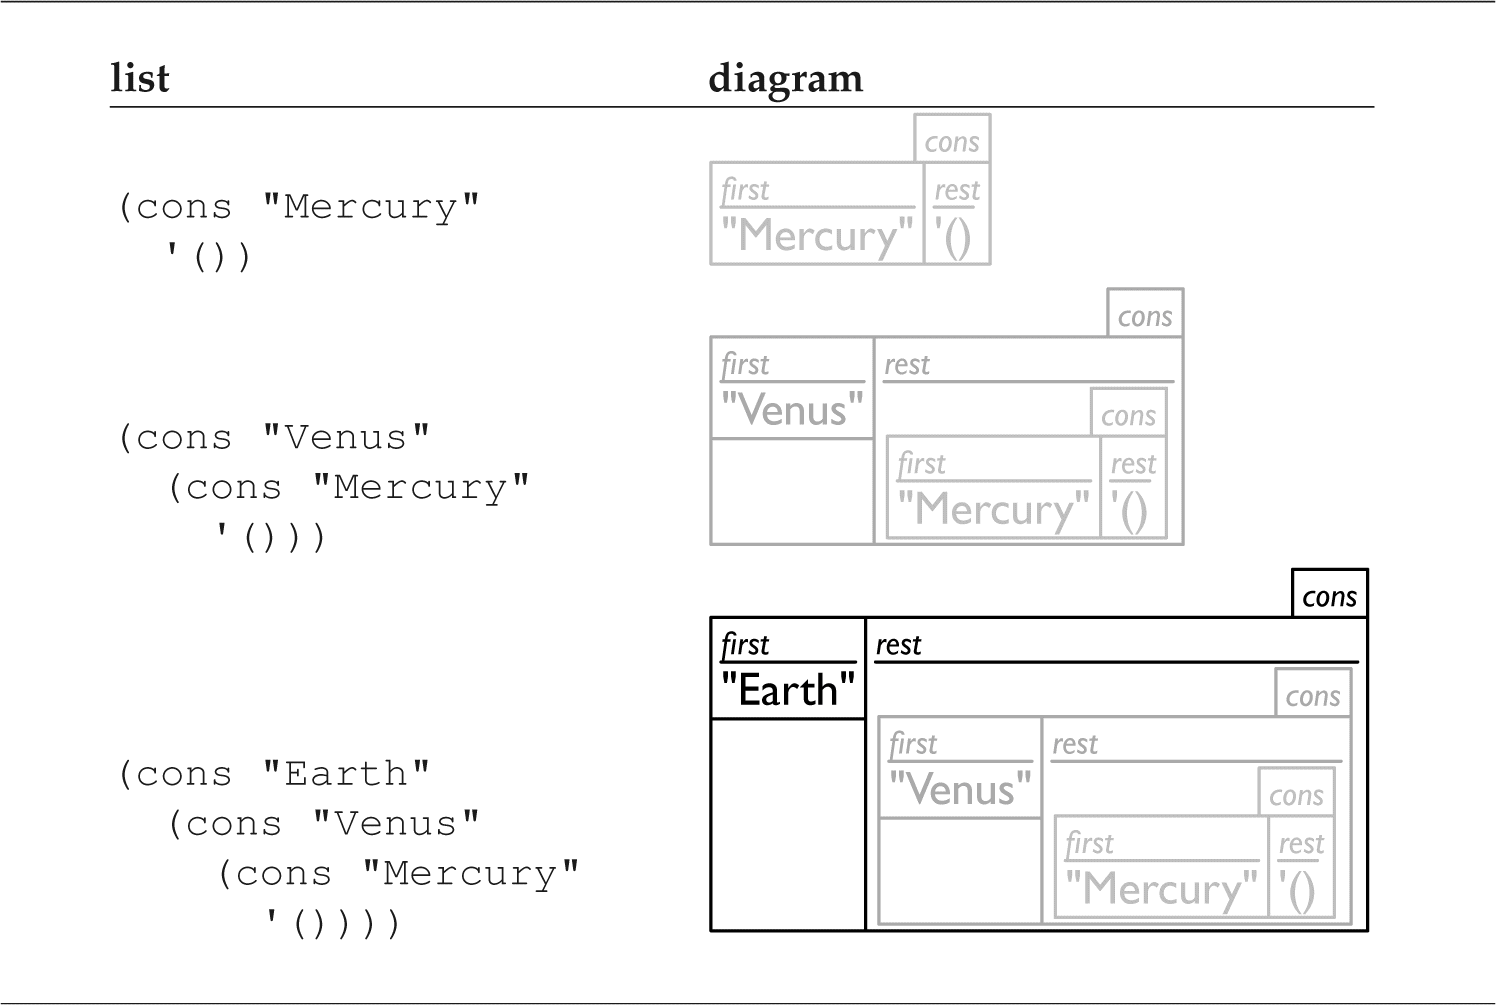
\includegraphics[width=0.75\textwidth]{images/00164.png}
  \caption{构建列表}
  \label{fig:building_a_list}
\end{figure}

一旦有了一个包含单个元素的列表，我们就可以再次使用 \code{cons} 来构造包含两个元素的列表。例如：
\begin{lstlisting}[language=BSL]
(cons "Venus" (cons "Mercury" '()))
\end{lstlisting}
再如：
\begin{lstlisting}[language=BSL]
(cons "Earth" (cons "Mercury" '()))
\end{lstlisting}

图~\ref{fig:building_a_list} 的中间一行展示了如何想象包含两个元素的列表。它同样是一个具有两个字段的方框，但此时其 \code{rest} 字段中包含着另一个方框。实际上，它所包含的正是在同一张图中上一行所示的方框。

最后，我们构造一个包含三个元素的列表：
\begin{lstlisting}[language=BSL]
(cons "Earth" (cons "Venus" (cons "Mercury" '())))
\end{lstlisting}

图~\ref{fig:building_a_list} 的最后一行展示了这个三元素列表。其 \code{rest} 字段包含一个方框，而该方框中又嵌套着另一个方框。因此，随着我们创建列表，我们实际上是在“大盒套中盒，中盒套小盒”。初看之下这或许有些奇特，但它就像俄罗斯套娃或我们生日时收到的层层嵌套的礼物盒。唯一的区别在于，BSL 程序中列表嵌套的深度，远胜于任何工匠能制造的物理套盒。

由于即便是高超的画师也很难手绘极深嵌套的结构，计算机科学家改用\term{盒与箭头图}（box-and-arrow diagrams）。图~\ref{fig:drawing_a_list} 展示了如何重排图~\ref{fig:building_a_list} 的最后一行。每个 \code{cons} 结构变成一个独立的方框。如果 \code{rest} 字段过于复杂无法直接在方框内画出，我们就画一个圆点，并引出一条带箭头的线指向它所包含的方框。根据方框的排布方式，可以得到两类图示：图~\ref{fig:drawing_a_list} 顶行展示的是按照方框\textbf{创建的先后顺序}排列的；底行展示的则是按照它们被 \code{cons} \textbf{组合的逻辑顺序}排列的。因此，第二种图示能让你一目了然地看出对该列表调用 \code{first} 会得到什么，无论列表有多长。出于这个原因，程序员更青睐第二种排布方式。

\begin{figure}[htbp]
  \centering
  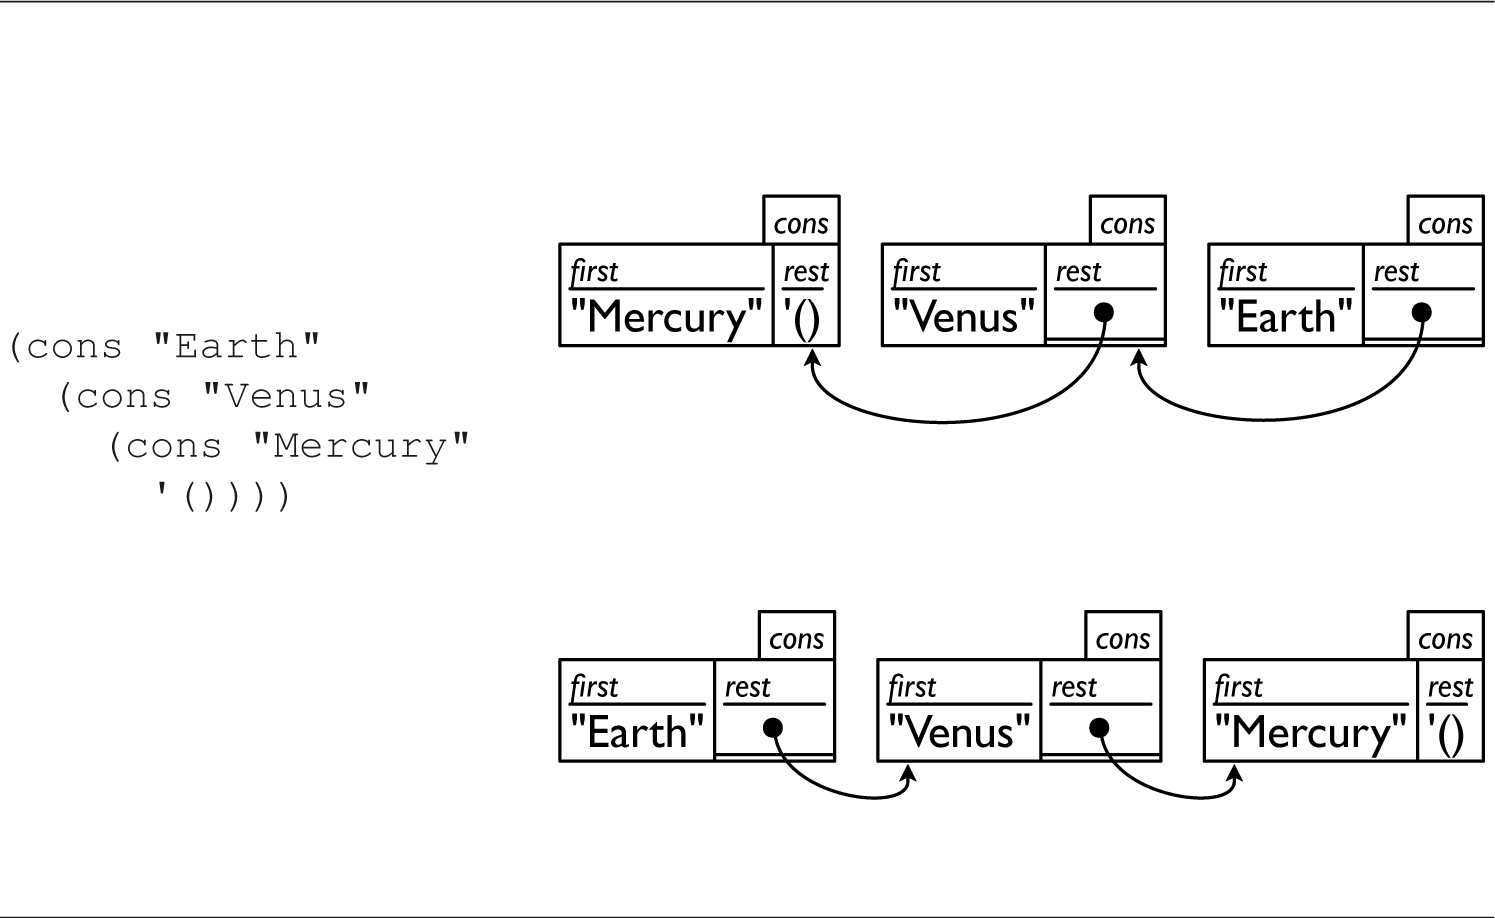
\includegraphics[width=0.75\textwidth]{images/00165.png}
  \caption{绘制列表}
  \label{fig:drawing_a_list}
\end{figure}

\begin{exercise}{创建基础列表}{129}
创建表示下列内容的 BSL 列表：
\begin{enumerate}
  \item 天体列表，至少包含太阳系中的所有行星；
  \item 一餐的食物清单，例如：牛排（steak）、薯条（french fries）、豆子（beans）、面包（bread）、水（water）、布里奶酪（Brie cheese）以及冰淇淋（ice cream）；
  \item 颜色列表。
\end{enumerate}
参考图~\ref{fig:building_a_list} 和图~\ref{fig:drawing_a_list}，绘制这些列表的方框图表示。你更喜欢哪种绘制方式？
\end{exercise}

你也可以创建数字列表。下面是一个包含 10 个一位数字（0 到 9）的列表：
\begin{lstlisting}[language=BSL]
(cons 0
  (cons 1
    (cons 2
      (cons 3
        (cons 4
          (cons 5
            (cons 6
              (cons 7
                (cons 8
                  (cons 9 '()))))))))))
\end{lstlisting}

构建这个列表需要 10 次 \code{cons} 构造以及一个 \code{'()}。对于一个包含三个任意数字的列表，例如：
\begin{lstlisting}[language=BSL]
(cons 1 (cons 2 (cons 3 '())))
\end{lstlisting}
我们需要三次 \code{cons}。

一般而言，列表并不要求所包含的值都是同一种类型，它可以包含任意类型的值：
\begin{lstlisting}[language=BSL]
(cons "Robin" (cons 12 (cons #true '())))
\end{lstlisting}

这个列表的第一个元素是字符串，第二个是数字，最后一个是布尔值。你可以将此列表视作一条包含三项数据的人事记录：雇员姓名、在公司的工龄、以及雇员是否通过公司加入了医疗保险。或者，你也可以将其视为游戏中虚拟玩家的某种状态。如果没有数据定义，你根本无从得知这些数据究竟代表什么。

\begin{notebox}[结构体 vs 列表]
如果某个数据用于表示包含\textbf{固定数量}组件的信息记录，应该优先使用结构体（structure type）；如果数据包含的项数是\textbf{任意大小}的，才应该使用列表。
\end{notebox}

下面是一个涉及 \code{cons} 的最初步的数据定义：
\begin{lstlisting}[language=BSL]
; 3LON 是包含三个数字的列表：
;   (cons Number (cons Number (cons Number '())))
; 解释：三维空间中的一个点
\end{lstlisting}

当然，这个数据定义使用 \code{cons} 的方式与使用结构体构造器并无二致，在某种意义上，\code{cons} 就是一个特殊的构造器。但该定义未能展示的是：如何形成\textbf{任意长度}的列表——包含 0 个项、1 个项、2 个项、10 个项，抑或 1,438,901 个项的列表。

让我们再做一次尝试：
\begin{lstlisting}[language=BSL]
; List-of-names 是以下之一：
; -- '()
; -- (cons String List-of-names)
; 解释：按姓氏排列的受邀宾客名单
\end{lstlisting}

深吸一口气，再仔细读一遍。这是你遇到过的最不同寻常的定义之一——在此之前，你从未见过一个\textbf{引用自身}的定义。它甚至看起来令人怀疑是否讲得通。毕竟，如果你对语文老师说“桌子就是桌子”来定义“桌子”，最可能得到的回答是“荒谬！”，因为自引用定义并没有阐明一个词汇的含义。

然而，在计算机科学和程序设计中，自引用定义扮演着核心角色；只要稍加严谨规范，此类定义是完全合情合理的。在这里，“合情合理”意味着我们可以将此数据定义用于其既定目的：生成属于该定义类别的\textbf{数据示例}，或者检查给定的某块数据是否属于所定义的类别。从这个角度来看，\code{List-of-names} 的定义完全经得起检验：
\begin{itemize}
  \item 首先，根据分项分类中的第一条分支，我们可以生成 \code{'()} 作为第一个例子。
  \item 有了 \code{'()} 作为 \code{List-of-names} 的一个已知元素，利用第二条分支很容易构造出第二个例子：
\begin{lstlisting}[language=BSL]
(cons "Findler" '())
\end{lstlisting}
  这里我们使用了字符串 \code{"Findler"} 和已确认为 \code{List-of-names} 的 \code{'()}，根据第二条规则生成了一个新的数据。
  \item 依此类推，我们可以生成更多此类单元素列表：
\begin{lstlisting}[language=BSL]
(cons "Flatt" '())
(cons "Felleisen" '())
(cons "Krishnamurthi" '())
\end{lstlisting}
  \item 虽然上述列表都只包含一个名字，但根据第二条规则，我们完全可以使用已有的单元素列表来生成包含更多名字的列表：
\begin{lstlisting}[language=BSL]
(cons "Felleisen" (cons "Findler" '()))
\end{lstlisting}
  这段数据属于 \code{List-of-names}，因为 \code{"Felleisen"} 是一个字符串，而 \code{(cons "Findler" '())} 已被证实属于 \code{List-of-names}。
\end{itemize}

\begin{exercise}{宾客名单验证}{130}
创建一个属于 \code{List-of-names} 且包含 5 个字符串的元素。参考图~\ref{fig:building_a_list} 绘制该列表的方框图表示。

请解释为什么：
\begin{lstlisting}[language=BSL]
(cons "1" (cons "2" '()))
\end{lstlisting}
是 \code{List-of-names} 的一个元素，而 \code{(cons 2 '())} 则不是。
\end{exercise}

\begin{exercise}{布尔值列表的数据定义}{131}
为表示布尔值列表给出数据定义。该类别包含任意长度的布尔值列表。
\end{exercise}

\section{什么是 '()，什么是 cons}
\label{sec:ch08_what_is_empty_and_cons}

让我们稍作停顿，仔细审视 \code{'()} 和 \code{cons}。正如前面提到的，\code{'()} 只是一个常量。与 \code{5} 或 \code{"this is a string"} 等常量相比，它看起来更像是一个函数名或变量；但若与 \code{\#true} 和 \code{\#false} 相比，就不难看出它确实只是 BSL 中用于表示空列表的符号常量。

在我们之前的求值规则中，\code{'()} 是一种全新的\textbf{原子值}（atomic value），与数字、布尔值、字符串等任何其他类型截然不同。它也不是复合值（如 \code{posn}）。事实上，\code{'()} 是如此独特，以至于它自身构成了一个独立的数值类别。因此，该类别配备了一个专用的谓词，仅识别 \code{'()} 而不识别任何其他值：
\begin{lstlisting}[language=BSL]
; Any -> Boolean
; 判断给定值是否为 '()
(define (empty? x) ...)
\end{lstlisting}

如同所有谓词一样，\code{empty?} 可以应用于 BSL 值世界中的任何值。当且仅当应用于 \code{'()} 时，它产生 \code{\#true}：
\begin{replbox}
> (empty? '())
#true
> (empty? 5)
#false
> (empty? "hello world")
#false
> (empty? (cons 1 '()))
#false
> (empty? (make-posn 0 0))
#false
\end{replbox}

接下来我们转向 \code{cons}。目前所见的一切都在提示：\code{cons} 是一个构造器，就像结构体类型定义所引入的构造器一样。更准确地说，\code{cons} 似乎是一个具有两个字段的结构体的构造器：第一个字段存放任意类型的值，第二个字段存放类似列表的值。以下定义将这一思想转换为 BSL 代码：
\begin{lstlisting}[language=BSL]
(define-struct pair [left right])

; ConsPair 是一个结构体：
;   (make-pair Any Any)

; Any Any -> ConsPair
(define (our-cons a-value a-list)
  (make-pair a-value a-list))
\end{lstlisting}

唯一的区别在于，\code{our-cons} 的第二个参数接受所有可能的 BSL 值，而真正的 \code{cons} 则不然，如下面的交互实验所示：
\begin{replbox}
> (cons 1 2)
cons: second argument must be a list, but received 1 and 2
\end{replbox}

换言之，\code{cons} 实际上是一个\term{带类型检查的函数}（checked function，如第 6 章所述）。这促使我们对定义进行细化：
\begin{lstlisting}[language=BSL]
; ConsOrEmpty 是以下之一：
; -- '()
; -- (make-pair Any ConsOrEmpty)
; 解释：ConsOrEmpty 是所有列表构成的类别

; Any Any -> ConsOrEmpty
(define (our-cons a-value a-list)
  (cond
    [(empty? a-list) (make-pair a-value a-list)]
    [(pair? a-list) (make-pair a-value a-list)]
    [else (error "cons: second argument must be a list")]))
\end{lstlisting}

既然 \code{cons} 是一个带类型检查的构造函数，你可能会好奇该如何从生成的结构体中提取各个部分。毕竟第 5 章曾说明，针对结构体编程必须借助选择器（selector）。由于 \code{cons} 结构有两个字段，因此存在两个选择器：\code{first} 和 \code{rest}。它们同样很容易基于我们的 \code{pair} 结构体来定义：
\begin{lstlisting}[language=BSL]
; ConsOrEmpty -> Any
; 提取列表的首元素
(define (our-first a-list)
  (if (empty? a-list)
      (error "first: expects a non-empty list")
      (pair-left a-list)))

; ConsOrEmpty -> ConsOrEmpty
; 提取列表除首元素外的其余部分
(define (our-rest a-list)
  (if (empty? a-list)
      (error "rest: expects a non-empty list")
      (pair-right a-list)))
\end{lstlisting}

请停下来思考片刻，自行定义 \code{our-rest}！

如果你的程序能够直接访问 \code{pair} 结构体的定义，就很容易构造出在 \code{right} 字段中既不包含 \code{'()} 也不包含另一个 \code{pair} 的非法实例。无论这种不良实例是故意还是无意创建的，它们往往会以怪异的方式破坏函数和程序。因此，BSL 特意隐藏了 \code{cons} 底层的结构体类型定义以避免这些问题。

图~\ref{fig:list_primitives} 总结了本节的核心内容。关键洞见在于：\code{'()} 是一个独一无二的原子值，而 \code{cons} 是一个产生列表值的带类型校验构造器。此外，\code{first}、\code{rest} 和 \code{cons?} 不过是常规谓词和选择器的特殊命名。因此，本章所讲授的并非一种创造数据的新方式，而是一种\textbf{阐明数据定义的新方式}。

\begin{figure}[htbp]
  \centering
  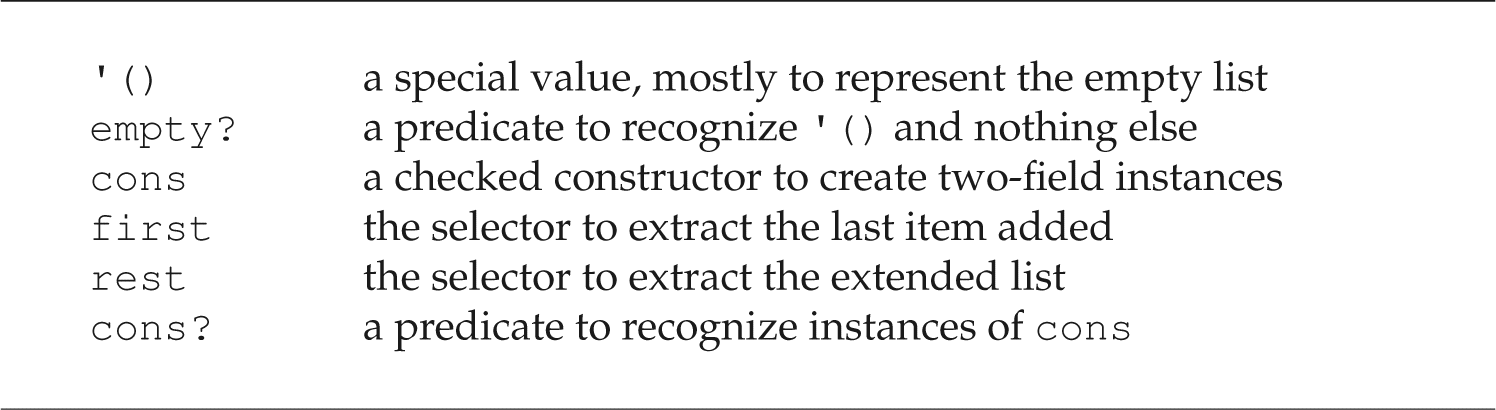
\includegraphics[width=0.8\textwidth]{images/00170.png}
  \caption{列表基本原语}
  \label{fig:list_primitives}
\end{figure}

\section{针对列表编程}
\label{sec:ch08_programming_with_lists}

假设你正在用一个列表记录你的朋友名单，并且这个列表已经变得非常庞大，以至于你需要一个程序来判断某个名字是否在名单中。为了让这一想法具象化，我们将其表述为一个例题：

\begin{notebox}[应用场景例题]
你正在为一款新手机开发通讯录功能。手机用户会在各种场合更新和查阅该通讯录。当前你的任务是：设计一个函数，接受该联系人列表，并判断其中是否包含名字 \code{"Flatt"}。
\end{notebox}

一旦解决了这个例题，我们便可将其推广为一个能在列表中查找\textbf{任意}名字的通用函数。

上一节中的 \code{List-of-names} 数据定义恰好适合用来表示待搜索的名字列表。接下来完成函数的前期材料（签名、目的说明和桩函数）：
\begin{lstlisting}[language=BSL]
; List-of-names -> Boolean
; 判断 "Flatt" 是否出现在 a-list-of-names 中
(define (contains-flatt? a-list-of-names)
  #false)
\end{lstlisting}

虽然 \code{a-list-of-names} 能准确表达输入参数的含义，但略显冗长，因此我们通常将其简写为 \code{alon}。

按照设计配方的常规步骤，接下来构造能够体现函数目的的示例。首先考虑最简单的输入：空列表 \code{'()}。既然该列表不包含任何字符串，它显然不包含 \code{"Flatt"}：
\begin{lstlisting}[language=BSL]
(check-expect (contains-flatt? '()) #false)
\end{lstlisting}

然后考虑只包含单个元素的列表：
\begin{lstlisting}[language=BSL]
(check-expect (contains-flatt? (cons "Findler" '())) #false)
(check-expect (contains-flatt? (cons "Flatt" '())) #true)
\end{lstlisting}
在第一种情况下，结果为 \code{\#false}，因为列表中的唯一元素并非 \code{"Flatt"}；在第二种情况下结果为 \code{\#true}。

最后，给出一个更通用的多元素列表示例：
\begin{lstlisting}[language=BSL]
(check-expect (contains-flatt? (cons "A" (cons "Flatt" (cons "C" '())))) #true)
\end{lstlisting}
停下来思考一下：请构造一个包含多个名字但返回值为 \code{\#false} 的示例！

停下来深吸一口气，运行一下测试。函数头是一个“桩”（dummy）定义；你构造了示例并转成了测试；更棒的是，其中某些测试居然通过了！虽然它们通过的原因纯属巧合，但确实通过了。如果一切清晰，请继续往下读。

第四步是根据数据定义设计\term{函数模板}（template）。因为字符串列表的数据定义包含\textbf{两个分支}，所以函数体必须是一个包含\textbf{两个分支}的 \code{cond} 表达式。这两个条件用于确定函数接收到的是哪一类列表：
\begin{lstlisting}[language=BSL]
(define (contains-flatt? alon)
  (cond
    [(empty? alon) ...]
    [(cons? alon) ...]))
\end{lstlisting}
在第二个分支中，我们也可以使用 \code{else} 代替 \code{(cons? alon)}。

我们可以通过依次考察每个 \code{cond} 分支为模板增加更多提示信息。具体而言，设计配方建议：如果对应的输入类别由复合数据构成，则在该分支中列出所有的选择器表达式。在我们的例子中，\code{'()} 不包含组件；而非空列表由一个字符串和另一个字符串列表构成。因此，我们在模板中加入 \code{(first alon)} 和 \code{(rest alon)}：
\begin{lstlisting}[language=BSL]
(define (contains-flatt? alon)
  (cond
    [(empty? alon) ...]
    [(cons? alon)
     (... (first alon) ... (rest alon) ...)]))
\end{lstlisting}

现在进入第五步：编写函数体。我们从模板出发，逐个处理每个 \code{cond} 分支：
\begin{itemize}
  \item 如果 \code{(empty? alon)} 为真，输入为空列表，函数必须产生 \code{\#false}。
  \item 第二个分支中 \code{(cons? alon)} 为真。模板提醒我们存在第一个字符串 \code{(first alon)} 以及列表的其余部分 \code{(rest alon)}。考察形如下式的例子：
\begin{lstlisting}[language=BSL]
(cons "A" (cons ... '()))
\end{lstlisting}
  函数就像人类一样，必须将第一个元素与 \code{"Flatt"} 进行比较。在此例中第一个是 \code{"A"} 而非 \code{"Flatt"}，因此比较结果为 \code{\#false}。如果第一个元素是 \code{"Flatt"}，则比较结果为 \code{\#true}。这意味着 \code{cond} 的第二行应该包含比较首元素是否等于 \code{"Flatt"} 的表达式：
\begin{lstlisting}[language=BSL]
(string=? (first alon) "Flatt")
\end{lstlisting}
\end{itemize}

此外，如果该比较得到 \code{\#true}，函数可以直接返回 \code{\#true}；如果比较结果为 \code{\#false}，我们还剩下列表的其余部分：\code{(rest alon)}。显然，此时函数还无法得出最终结论，因为答案取决于后续元素是什么。换言之，如果首元素不是 \code{"Flatt"}，我们需要某种方法来检查\textbf{列表的其余部分是否包含 \code{"Flatt"}}。

幸运的是，我们手里正有 \code{contains-flatt?}，它完全符合要求！根据其目的说明，它能判断一个列表是否包含 \code{"Flatt"}。这意味着 \code{(contains-flatt? (rest alon))} 能够准确判断 \code{"Flatt"} 是否存在于 \code{(rest alon)} 中——这正是我们迫切需要知道的！

因此，最后一行应当包含 \code{(contains-flatt? (rest alon))}：
\begin{lstlisting}[language=BSL]
(define (contains-flatt? alon)
  (cond
    [(empty? alon) #false]
    [(cons? alon)
     (... (string=? (first alon) "Flatt") ...
      ... (contains-flatt? (rest alon)) ...)]))
\end{lstlisting}

接下来的诀窍就是以适当的方式将这两个表达式的值组合起来。如前所述，如果第一个表达式产生 \code{\#true}，就没有必要继续搜索后续列表；但如果它是 \code{\#false}，第二个表达式仍可能产生 \code{\#true}（意味着名字出现在剩余列表中）。这一切表明：当且仅当首元素匹配或者剩余列表包含该名字时，最终结果才为 \code{\#true}。因此，使用 \code{or} 进行组合：
\begin{lstlisting}[language=BSL]
(or (string=? (first alon) "Flatt")
    (contains-flatt? (rest alon)))
\end{lstlisting}

图~\ref{fig:searching_a_list} 展示了完整的定义。总体而言，它与本书第一部分中的定义并无太大差异：包含签名、目的说明、测试用例和函数定义。该函数唯一定义不同于以往之处在于\textbf{自引用}，即在 \code{define} 的函数体内部调用了 \code{contains-flatt?} 自身。但反过来想，数据定义本身就是自引用的，所以在函数中出现自引用也就理所当然了。

\begin{figure}[htbp]
  \centering
  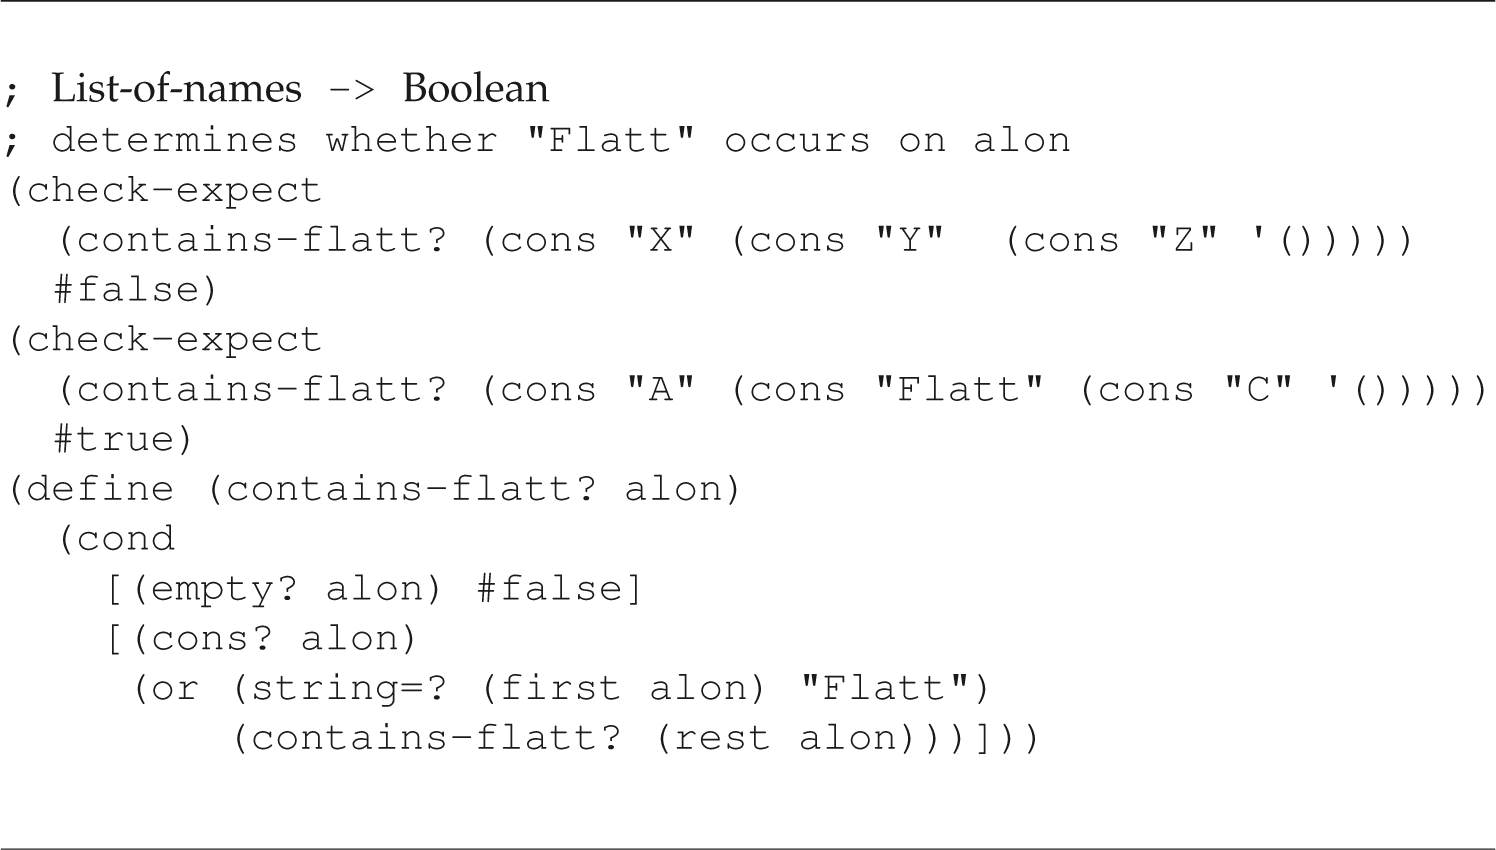
\includegraphics[width=0.85\textwidth]{images/00176.png}
  \caption{搜索列表}
  \label{fig:searching_a_list}
\end{figure}

\begin{exercise}{运行 contains-flatt?}{132}
在 DrRacket 中针对以下输入运行 \code{contains-flatt?}：
\begin{lstlisting}[language=BSL]
(cons "Fagan"
  (cons "Findler"
    (cons "Fisler"
      (cons "Flanagan"
        (cons "Flatt"
          (cons "Felleisen"
            (cons "Friedman" '())))))))
\end{lstlisting}
你预期的运行结果是什么？
\end{exercise}

\begin{exercise}{条件表达式的等价写法}{133}
下面是 \code{contains-flatt?} 中第二个 \code{cond} 分支的另一种表述方式：
\begin{lstlisting}[language=BSL]
(cond
  [(empty? alon) #false]
  [else
   (cond
     [(string=? (first alon) "Flatt") #true]
     [else (contains-flatt? (rest alon))])])
\end{lstlisting}
请解释为什么这个表达式与图~\ref{fig:searching_a_list} 中使用 \code{or} 的版本产生完全相同的结果。你认为哪个版本更好？请说明理由。
\end{exercise}

\begin{exercise}{通用查找函数 contains?}{134}
设计函数 \code{contains?}，判断给定的某个字符串是否出现在给定的字符串列表中。

\begin{notebox}[提示]
BSL 实际上内置了 \code{member?} 函数，它接受两个值并检查第一个值是否出现在作为列表的第二个值中：
\begin{replbox}
> (member? "Flatt" (cons "b" (cons "Flatt" '())))
#true
\end{replbox}
但在完成本练习时，\textbf{请不要}使用 \code{member?} 来定义 \code{contains?}。
\end{notebox}
\end{exercise}

\section{列表上的计算}
\label{sec:ch08_computing_with_lists}

由于我们仍在使用初学学生语言（BSL），代数求值规则（参见插曲 1）指导着我们如何在不借助 DrRacket 的情况下求出表达式的值，例如：
\begin{lstlisting}[language=BSL]
(contains-flatt? (cons "Flatt" (cons "C" '())))
\end{lstlisting}
程序员必须对此类代数演算过程拥有直观深刻的理解，因此我们逐步推演这个简单的例子。

图~\ref{fig:computing_with_lists_step1} 展示了第一步：应用常规的函数代换规则。结果是一个条件表达式，正如代数老师所说，该函数是以分段（step-wise）方式定义的。

\begin{figure}[htbp]
  \centering
  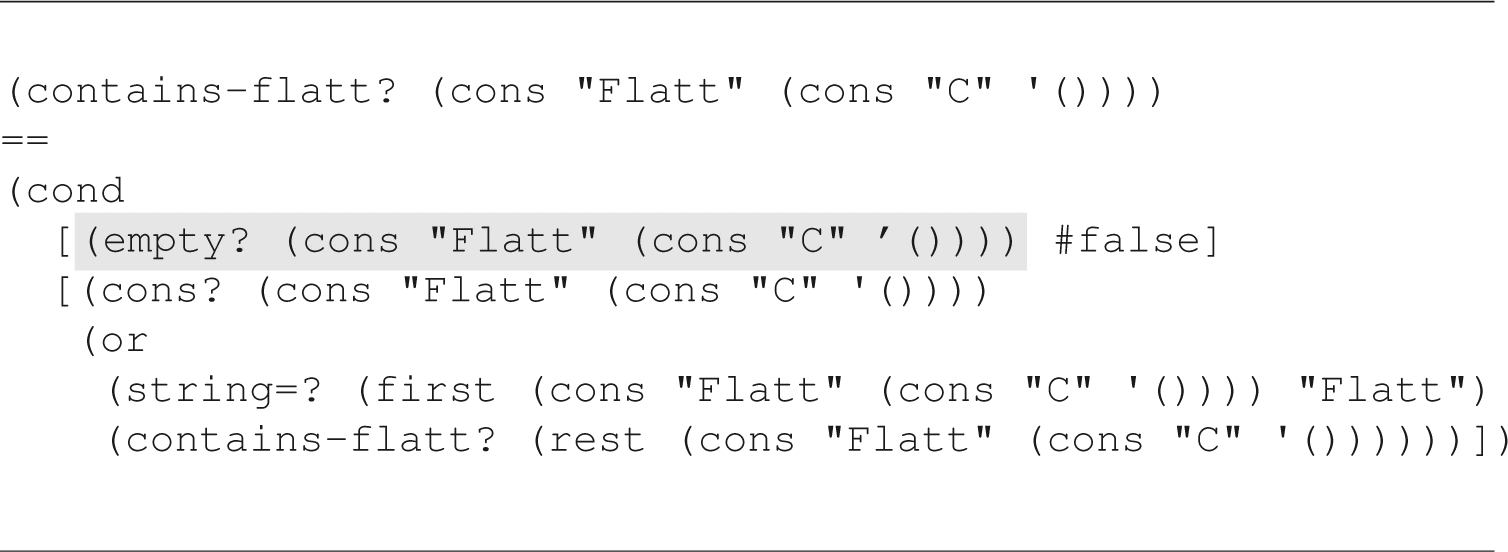
\includegraphics[width=0.85\textwidth]{images/00179.png}
  \caption{列表计算步骤 1}
  \label{fig:computing_with_lists_step1}
\end{figure}

图~\ref{fig:computing_with_lists_step2} 延续了这一演算过程。为了找到 \code{cond} 表达式的正确分支，我们必须逐一计算条件的值。由于 \code{cons} 构造出的列表不是空列表，第一个条件的值为 \code{\#false}，因此消去第一个 \code{cond} 分支。最后，第二个分支的条件求值为 \code{\#true}，因为对一个 \code{cons} 列表调用 \code{cons?} 必然成立。

\begin{figure}[htbp]
  \centering
  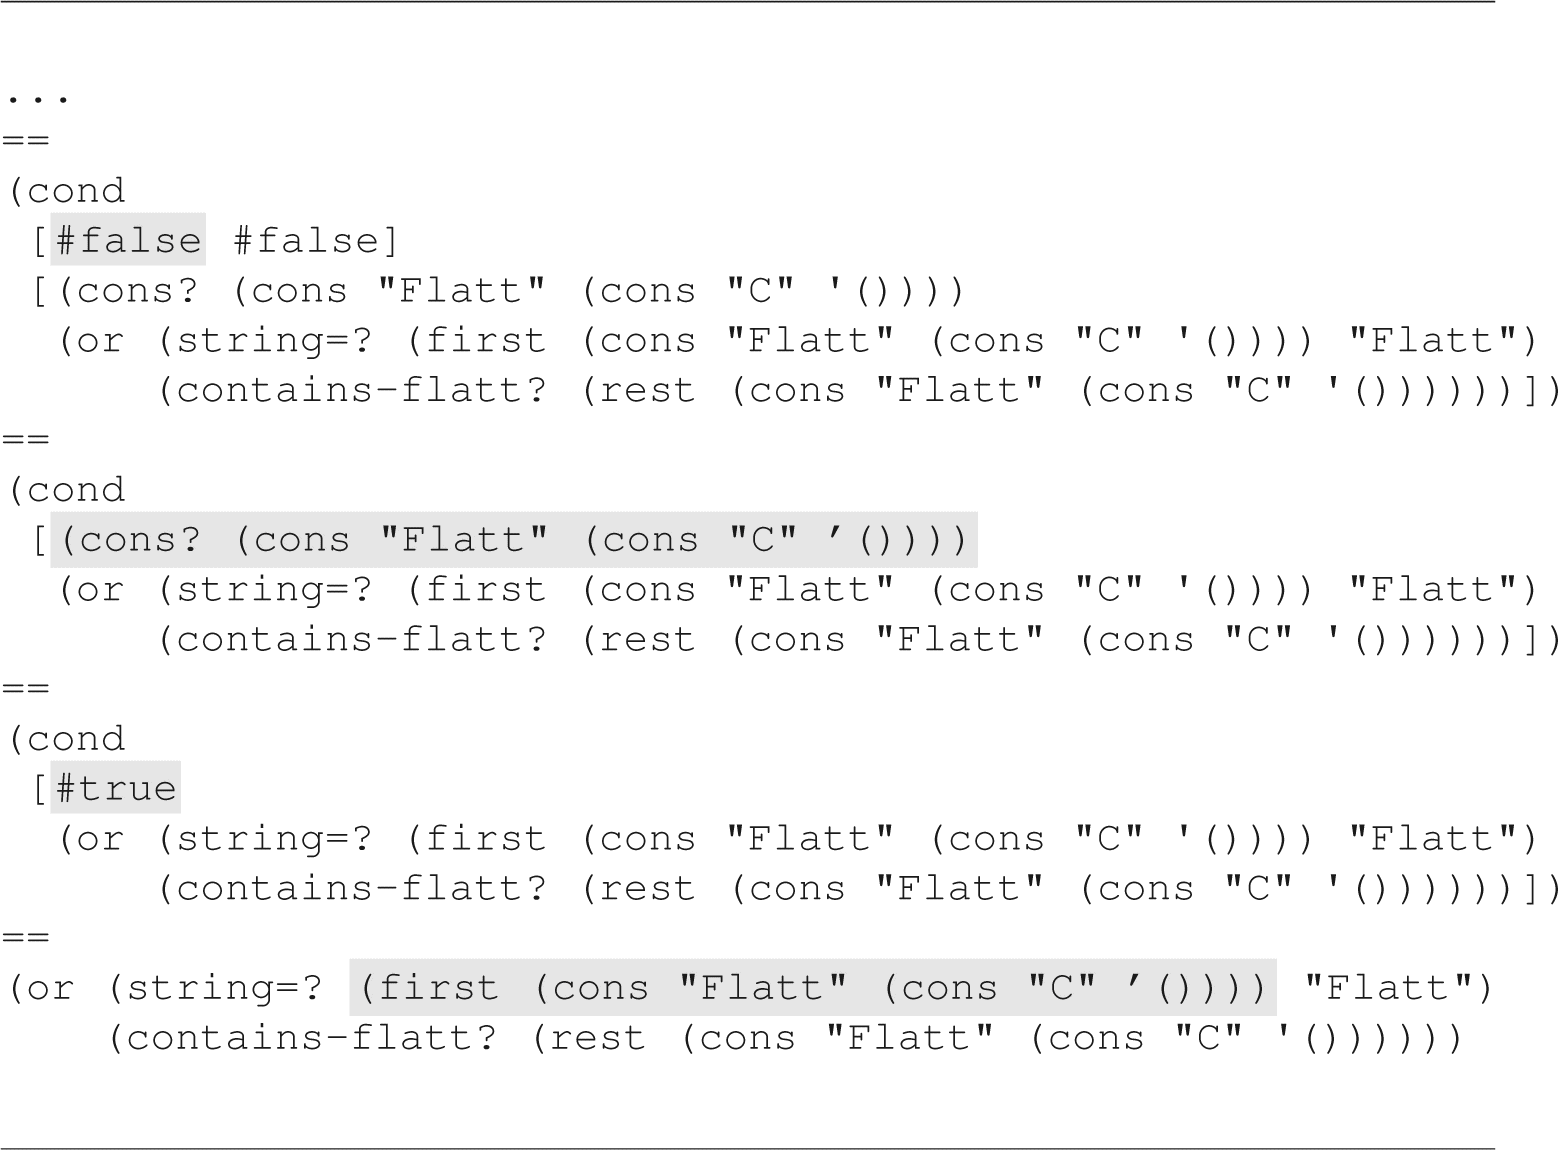
\includegraphics[width=0.85\textwidth]{images/00180.png}
  \caption{列表计算步骤 2}
  \label{fig:computing_with_lists_step2}
\end{figure}

从这里开始，仅需再经过三步基础算术化简即可得到最终结果。图~\ref{fig:computing_with_lists_step3} 展示了这三步：
\begin{enumerate}
  \item 根据 \code{first} 的求值法则，\code{(first (cons "Flatt" ...))} 被简化为 \code{"Flatt"}；
  \item 计算发现 \code{"Flatt"} 与 \code{"Flatt"} 确实是相等的字符串；
  \item 根据 \code{or} 的短路求值法则，无论表达式 $X$ 为何值，\code{(or \#true $X$)} 的结果都是 \code{\#true}。
\end{enumerate}

\begin{figure}[htbp]
  \centering
  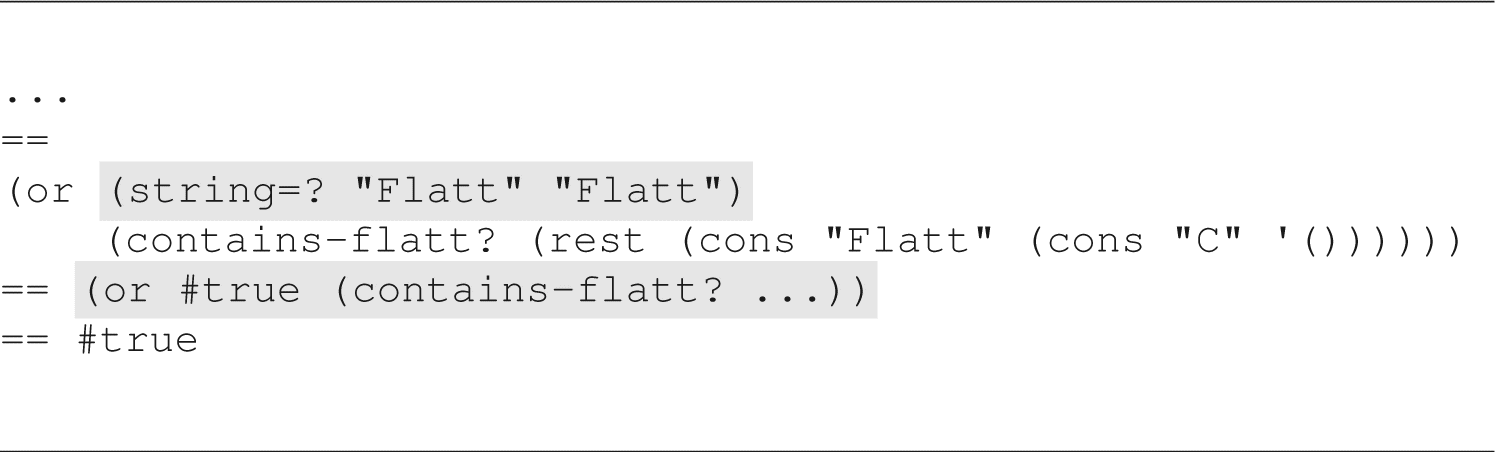
\includegraphics[width=0.85\textwidth]{images/00181.png}
  \caption{列表计算步骤 3}
  \label{fig:computing_with_lists_step3}
\end{figure}

\begin{exercise}{使用单步求值器观察 contains-flatt?}{135}
使用 DrRacket 的单步求值器（Stepper）单步观察以下表达式的计算过程：
\begin{lstlisting}[language=BSL]
(contains-flatt? (cons "Flatt" (cons "C" '())))
\end{lstlisting}
同时使用单步求值器观察下式的求值过程：
\begin{lstlisting}[language=BSL]
(contains-flatt? (cons "A" (cons "Flatt" (cons "C" '()))))
\end{lstlisting}
如果将 \code{"Flatt"} 替换为 \code{"B"} 会发生什么？
\end{exercise}

\begin{exercise}{验证列表原语选择器}{136}
利用 DrRacket 的单步求值器验证以下恒等关系：
\begin{lstlisting}[language=BSL]
(our-first (our-cons "a" '())) == "a"
(our-rest (our-cons "a" '())) == '()
\end{lstlisting}
有关这些函数的定义，请参见第 8.2 节。
\end{exercise}

% ==============================================================================
% 第 9 章：基于自引用数据定义进行设计 (Chapter 9: Designing with Self-Referential Data Definitions)
% ==============================================================================

\chapter{基于自引用数据定义进行设计}
\label{sec:ch09_designing_lists}

初看之下，自引用数据定义似乎比之前的混合数据定义复杂得多。但正如上一章 \code{contains-flatt?} 的例子所展示的那样，程序设计配方的六个基本步骤依然完全适用。在本章中，我们将推广并细化设计配方，使其能够更加自然流畅地应对自引用数据定义。新内容主要涉及三个方面：识别何时需要自引用数据定义、推导函数模板、以及编写函数体。

\begin{recipebox}{处理任意大小数据的设计配方}
\begin{enumerate}
  \item \textbf{数据定义}：如果问题陈述涉及\textbf{任意大小}的信息，就必须使用自引用数据定义来表示它。目前为止你只见过一种此类定义——\code{List-of-names}。图~\ref{fig:arrows_for_self_references} 左侧展示了以同样方式定义的 \code{List-of-strings}。其他原子数据的列表定义也遵循完全相同的规律。
  
  一个有效的自引用数据定义必须满足两个先决条件：
  \begin{itemize}
    \item 必须包含至少两个分支（clause）；
    \item 至少有一个分支\textbf{不能}引用正在定义的数据类别本身（即\term{基本情况/基准条件}，base case）。
  \end{itemize}
  良好的编程习惯是用箭头明确标出自引用关系：从数据定义内部的引用指回被定义术语本身（如图~\ref{fig:arrows_for_self_references} 所示）。

  你必须通过构造数据示例来检验自引用定义的有效性。先从不含自引用的分支开始生成第一个示例；接着使用包含自引用的分支，将前面生成的示例代入自引用位置以生成更大的示例：
\begin{lstlisting}[language=BSL]
'()
(cons "a" '())
(cons "b" (cons "a" '()))
\end{lstlisting}
  如果无法从数据定义生成示例，则该定义是无效的；如果你能生成示例但无法构造出规模递增的示例，则该定义可能无法契合其预期解释。

  \item \textbf{函数签名、目的说明与函数头}：函数头部材料与以往毫无二致：签名、目的说明和桩定义。在构思目的说明时，\textbf{务必关注函数计算什么，而非如何计算}，尤其不要过早考虑如何遍历给定的数据。例如：
\begin{lstlisting}[language=BSL]
; List-of-strings -> Number
; 计算 alos 中包含多少个字符串
(define (how-many alos)
  0)
\end{lstlisting}
  目的说明清晰指明了函数只负责统计字符串个数，无需预先设想如何在 BSL 中实现它。

  \item \textbf{功能示例}：在构思功能示例时，务必多次运用数据定义中的自引用分支来构造测试输入。这是后续确保测试用例覆盖整个函数定义的最佳途径：
\begin{lstlisting}[language=BSL]
(check-expect (how-many '()) 0)
(check-expect (how-many (cons "a" '())) 1)
(check-expect (how-many (cons "b" (cons "a" '()))) 2)
\end{lstlisting}

  \item \textbf{模板}：自引用数据定义本质上仍是分类数据定义，因此模板开发遵循第 6 章的规则。\code{cond} 表达式的分支数与数据定义的分支数完全一致；每个分支的条件对应数据定义的识别条件；在处理复合值的每个分支中写下相应的选择器表达式。
  
  图~\ref{fig:translate_data_def_to_template} 以问答形式阐明了这一过程。如果对消耗 \code{List-of-strings} 的函数应用这些规则，初步得到以下形态：
\begin{lstlisting}[language=BSL]
(define (fun-for-los alos)
  (cond
    [(empty? alos) ...]
    [(cons? alos)
     (... (first alos) ... (rest alos) ...)]))
\end{lstlisting}
  请牢记，模板的目的是将数据定义的结构转化为函数代码的骨架。当数据定义在第 $i$ 个分支的第 $k$ 个字段存在自引用时，模板就必须在第 $i$ 个分支对第 $k$ 个字段的选择器调用上建立\textbf{递归调用}！
  
  在文本代码中，我们通过函数的自调用（self-application）来代替箭头：
\begin{lstlisting}[language=BSL]
(define (fun-for-los alos)
  (cond
    [(empty? alos) ...]
    [(cons? alos)
     (... (first alos) ...
      ... (fun-for-los (rest alos)) ...)]))
\end{lstlisting}
  我们将函数的自我调用称为\term{递归}（recursion），在本书前四部分特称为\term{自然递归}（natural recursion）。

  \item \textbf{函数体编写}：从不含递归调用的分支（基本情况）开始编写，其答案通常显而易见或已在示例中给出。
  
  接着处理自引用分支。牢记模板中每个表达式计算的是什么。对于自然递归 \code{(fun-for-los (rest alos))}，\textbf{假定该函数已经按照目的说明正确工作}。这虽然看似是一次“信念之跃”（leap of faith），但它在数学归纳法（Induction Theorem）的保证下永远有效！剩下的工作只是将提取的值与递归调用的结果组合起来。

  \item \textbf{测试}：将所有示例转化为测试用例，确保全部通过，并检查测试覆盖了函数的所有分支。
\end{enumerate}
\end{recipebox}

\begin{figure}[htbp]
  \centering
  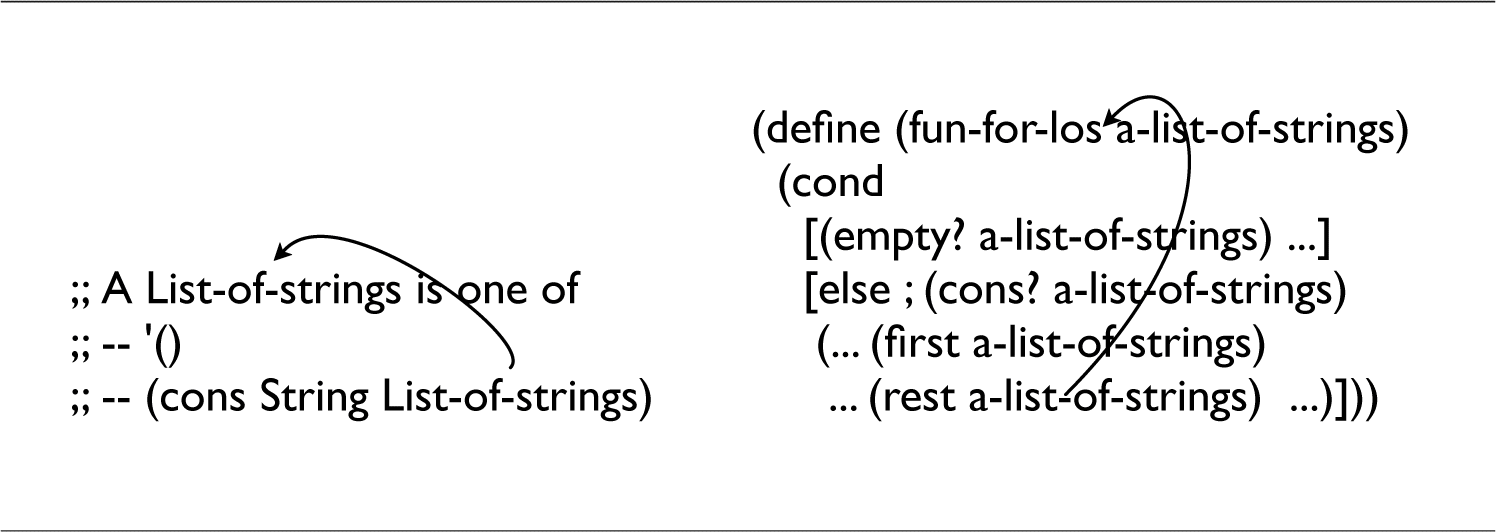
\includegraphics[width=0.85\textwidth]{images/00182.png}
  \caption{数据定义与模板中的自引用箭头映射}
  \label{fig:arrows_for_self_references}
\end{figure}

\begin{figure}[htbp]
  \centering
  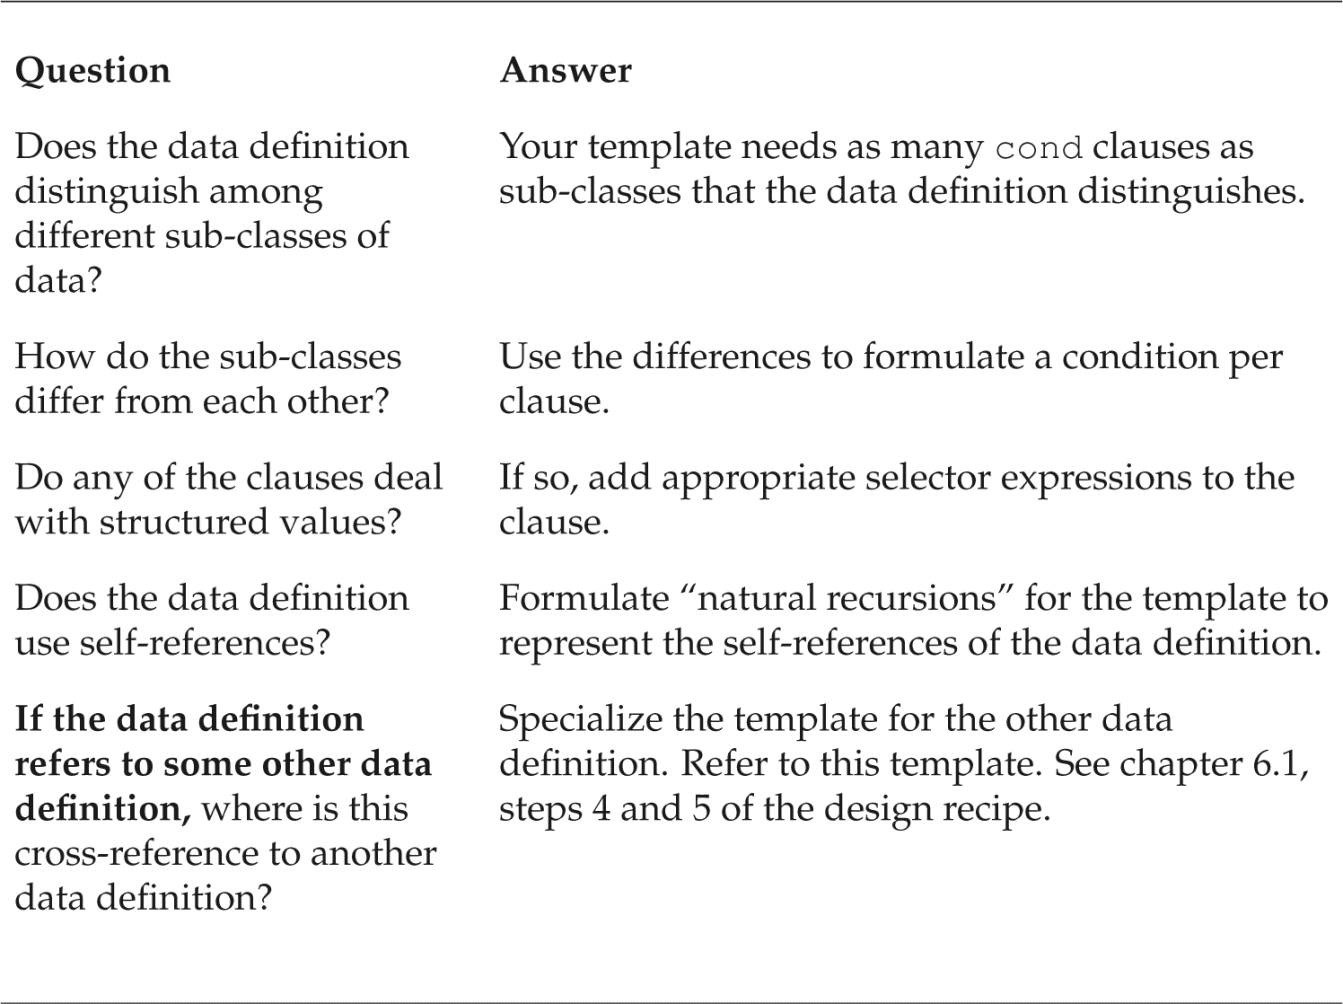
\includegraphics[width=0.85\textwidth]{images/00185.png}
  \caption{如何将数据定义转换为模板}
  \label{fig:translate_data_def_to_template}
\end{figure}

\begin{figure}[htbp]
  \centering
  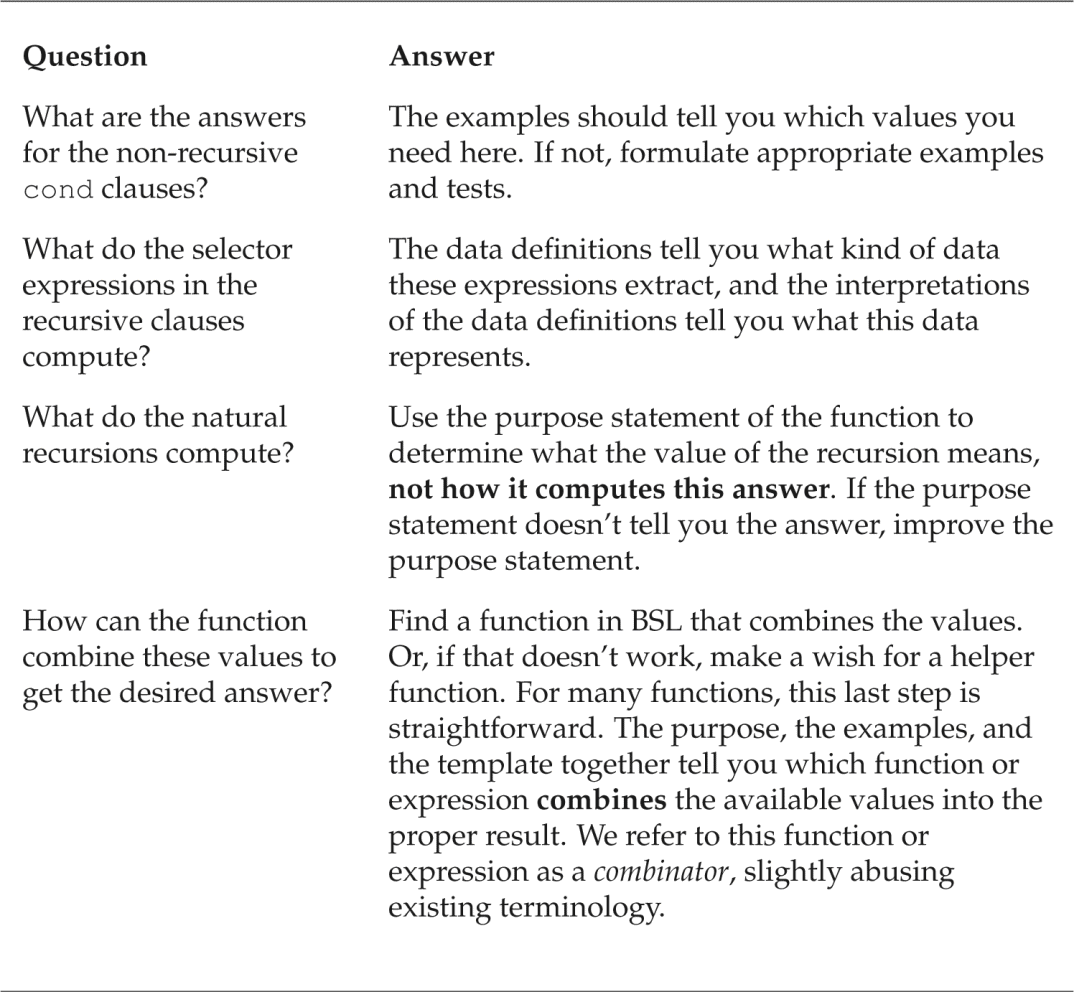
\includegraphics[width=0.85\textwidth]{images/00189.png}
  \caption{如何将模板转换为函数定义}
  \label{fig:turn_template_into_function}
\end{figure}

对于 \code{how-many}，基本情况为 \code{'()}，结果显然是 \code{0}。在第二分支中，\code{(first alos)} 得到首个字符串，\code{(how-many (rest alos))} 算出剩余列表的字符串个数。为了求出整个列表的长度，只需将递归结果加 \code{1}：
\begin{lstlisting}[language=BSL]
(define (how-many alos)
  (cond
    [(empty? alos) 0]
    [else (+ (how-many (rest alos)) 1)]))
\end{lstlisting}

\begin{notebox}[表格辅助法]
初学者在寻找组合函数（用于将首项与剩余项递归结果结合起来的辅助操作）时有时会感到困难。此时可以借助\term{表格辅助法}（如图~\ref{fig:table_method} 和图~\ref{fig:tabulating_args} 所示）：列出输入样例、模板中各子表达式的值以及期望的最终结果。观察自然递归列与期望结果列的数值差异，往往能一眼猜出所需的组合操作！
\end{notebox}

\begin{figure}[htbp]
  \centering
  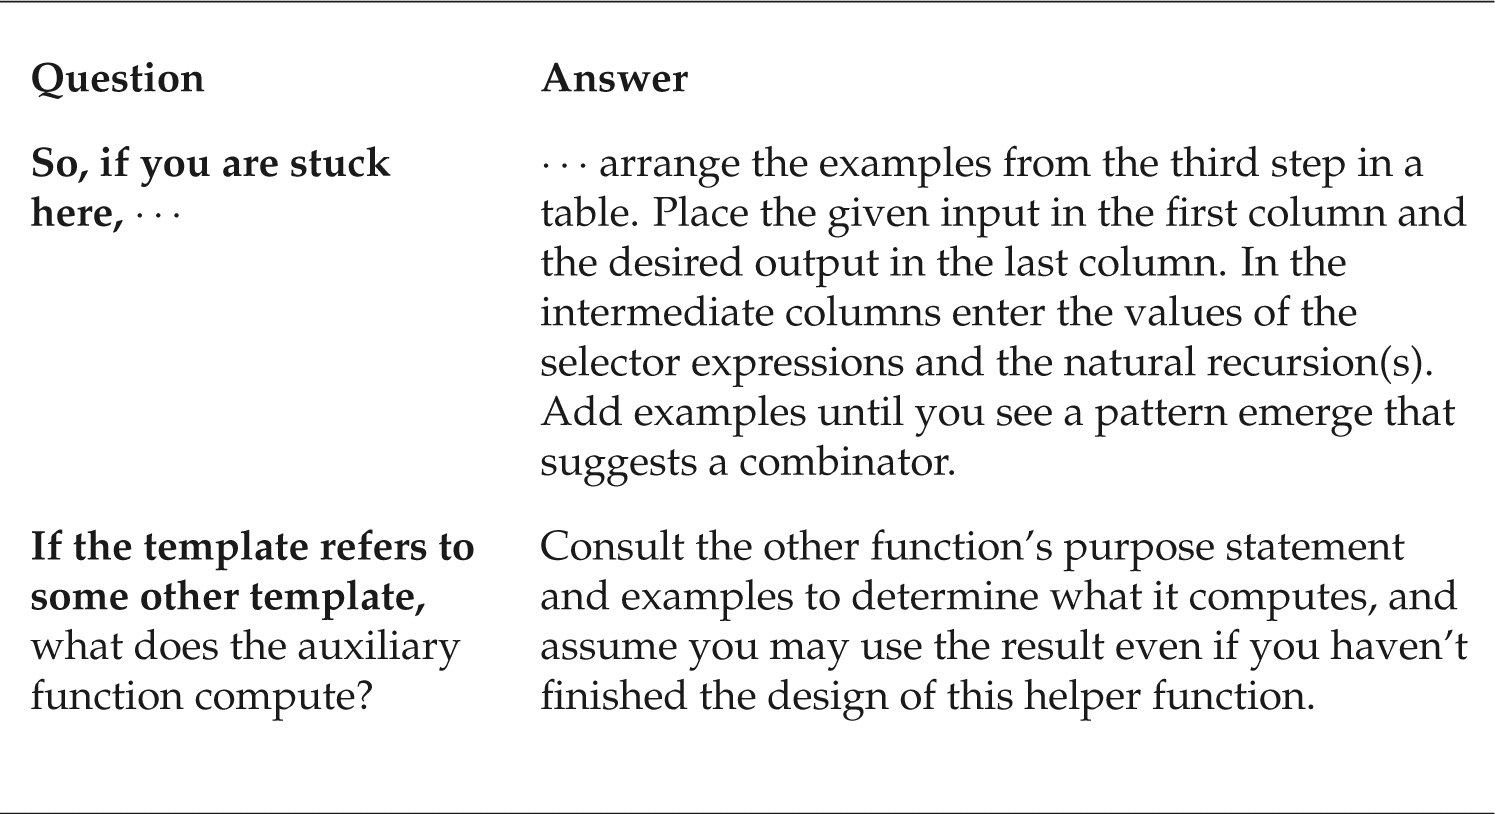
\includegraphics[width=0.8\textwidth]{images/00190.png}
  \caption{将模板转化为函数的表格方法}
  \label{fig:table_method}
\end{figure}

\begin{figure}[htbp]
  \centering
  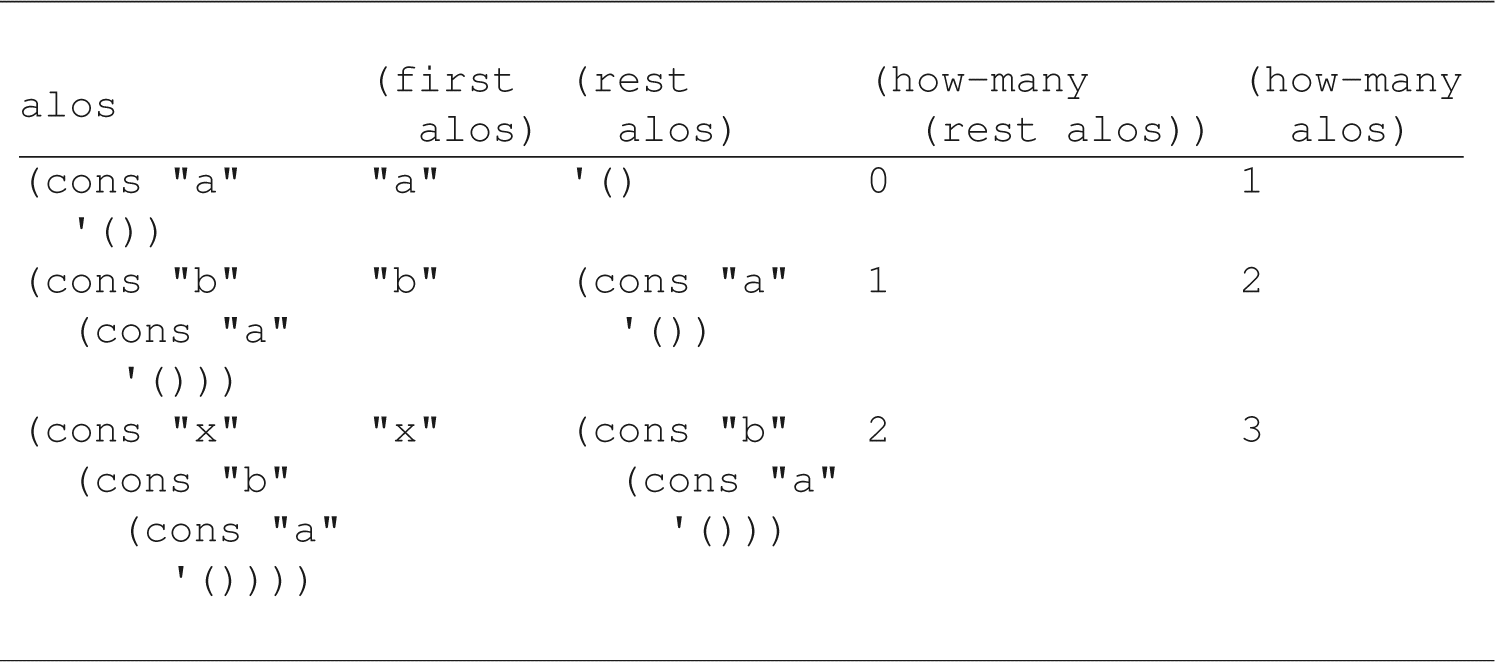
\includegraphics[width=0.8\textwidth]{images/00191.png}
  \caption{制表演算参数、中间值与结果}
  \label{fig:tabulating_args}
\end{figure}

图~\ref{fig:design_recipe_self_referential} 总结了针对自引用数据的完整设计配方表格。

\begin{figure}[htbp]
  \centering
  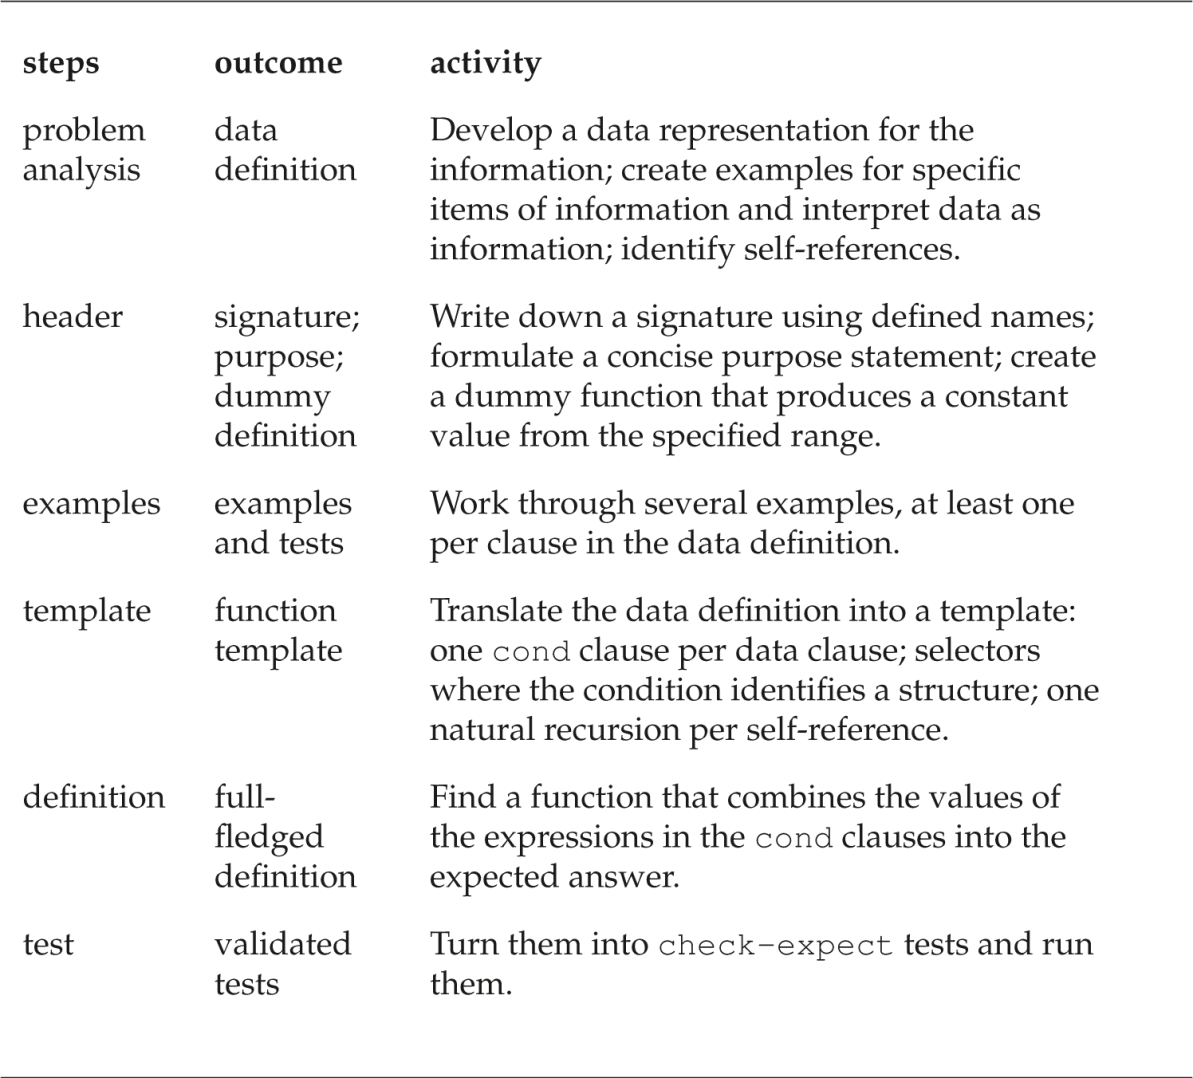
\includegraphics[width=0.9\textwidth]{images/00192.png}
  \caption{针对自引用数据设计函数的完整配方}
  \label{fig:design_recipe_self_referential}
\end{figure}

\section{练手习题：列表}
\label{sec:ch09_finger_exercises_lists}

\begin{exercise}{对比模板}{137}
比较 \code{contains-flatt?} 与 \code{how-many} 的模板。如果忽略函数名称，它们是完全相同的。请解释这种相似性的根源。
\end{exercise}

\begin{exercise}{金额求和函数 sum}{138}
以下是表示金额序列的数据定义：
\begin{lstlisting}[language=BSL]
; A List-of-amounts 是以下之一：
; -- '()
; -- (cons PositiveNumber List-of-amounts)
\end{lstlisting}
创建一些示例以确保你理解该数据定义，并在纸上画出标明自引用的箭头。

设计函数 \code{sum}，接收一个 \code{List-of-amounts} 并计算所有金额的总和。使用 DrRacket 的单步求值器观察 \code{(sum l)} 在短列表上的执行过程。
\end{exercise}

\begin{exercise}{数字列表验证与防御性求和}{139}
观察以下数据定义：
\begin{lstlisting}[language=BSL]
; A List-of-numbers 是以下之一：
; -- '()
; -- (cons Number List-of-numbers)
\end{lstlisting}
该类别的某些元素可以作为练习 138 中 \code{sum} 的合法输入，而另一些则不行。

设计函数 \code{pos?}，接收一个 \code{List-of-numbers} 并判断其中所有数字是否均为正数。换言之，若 \code{(pos? l)} 返回 \code{\#true}，则 \code{l} 同时也是 \code{List-of-amounts} 的元素。使用单步求值器观察 \code{pos?} 在 \code{(cons 5 '())} 和 \code{(cons -1 '())} 上的求值过程。

接着设计带校验的求和函数 \code{checked-sum}：接收一个 \code{List-of-numbers}。如果输入同时属于 \code{List-of-amounts}，则计算其总和；否则报错（提示：使用 \code{check-error} 进行测试）。

最后，思考如果直接对任意 \code{List-of-numbers} 应用练习 138 中的 \code{sum}，它会计算出什么？
\end{exercise}

\begin{exercise}{布尔值列表判定}{140}
设计函数 \code{all-true}，接收一个布尔值列表并判断其所有元素是否均为 \code{\#true}。也就是说，只要列表中存在任何 \code{\#false}，函数就返回 \code{\#false}。

接着设计函数 \code{one-true}，判断列表中是否至少有一个元素为 \code{\#true}。

在编写代码时尝试使用表格辅助法，它能帮你准确确定基本情况的返回值。使用单步求值器观察这些函数在 \code{(cons \#true '())}、\code{(cons \#false '())} 以及 \code{(cons \#true (cons \#false '()))} 上的运行轨迹。
\end{exercise}

\begin{exercise}{字符串拼接函数 cat}{141}
如果要设计函数 \code{cat}，接收一个字符串列表并将其拼接为一个长字符串，你必然会得到以下部分定义：
\begin{lstlisting}[language=BSL]
(define (cat los)
  (cond
    [(empty? los) ...]
    [else (... (first los) ... (cat (rest los)) ...)]))
\end{lstlisting}
完成图~\ref{fig:table_for_cat} 中的表格，猜出能够将子表达式的值组合为期望结果的函数。
使用单步求值器观察 \code{(cat (cons "a" '()))} 的求值。
\end{exercise}

\begin{figure}[htbp]
  \centering
  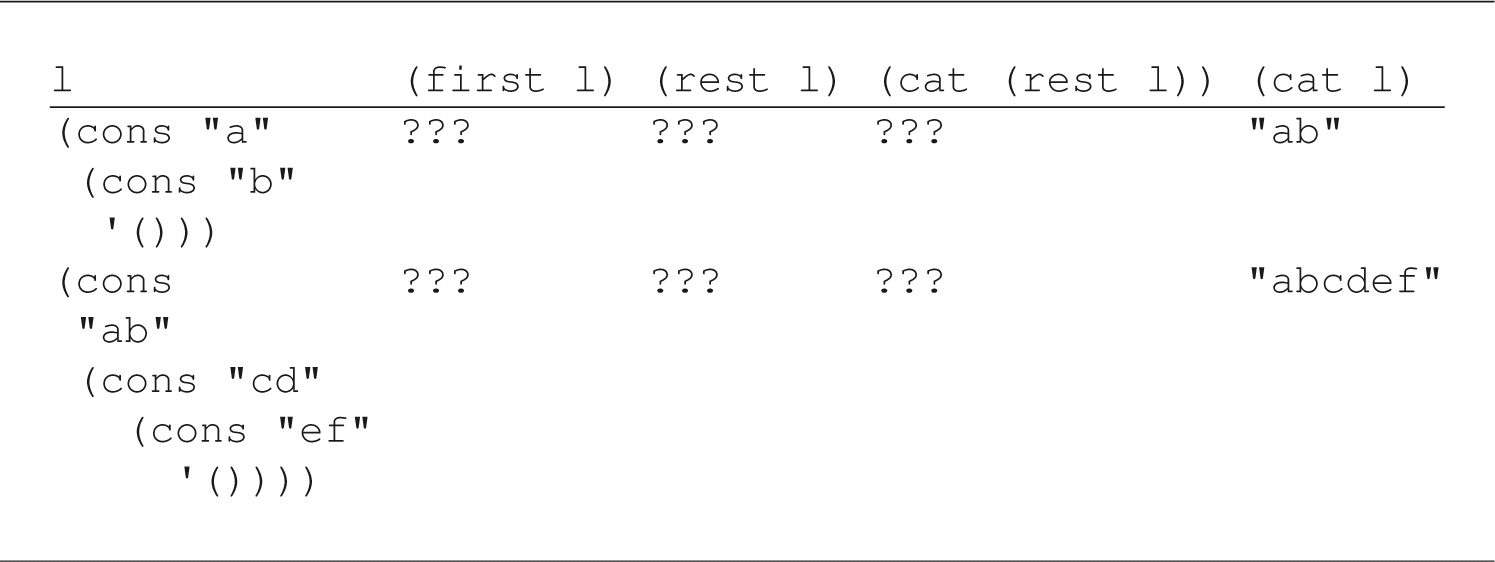
\includegraphics[width=0.8\textwidth]{images/00194.png}
  \caption{函数 cat 的辅助推导表}
  \label{fig:table_for_cat}
\end{figure}

\begin{exercise}{查找不合尺寸的图像 ill-sized?}{142}
设计函数 \code{ill-sized?}，消耗图像列表 \code{loi} 和一个正数 $n$。它返回 \code{loi} 中第一张\textbf{不是} $n \times n$ 正方形的图像；若所有图像均符合尺寸要求，则返回 \code{\#false}。

提示：在函数签名的结果部分使用以下数据定义：
\begin{lstlisting}[language=BSL]
; ImageOrFalse 是以下之一：
; -- Image
; -- #false
\end{lstlisting}
\end{exercise}

\section{非空列表}
\label{sec:ch09_non_empty_lists}

现在你已经掌握了使用 \code{cons} 以及构建列表数据定义的基础。本节我们将探讨一种在实践中极为常见的数据结构：\term{非空列表}（non-empty list）。

让我们从计算温度列表的平均值这一看似简单的问题开始：
\begin{lstlisting}[language=BSL]
; A List-of-temperatures 是以下之一：
; -- '()
; -- (cons CTemperature List-of-temperatures)

; A CTemperature 是大于 -272 的 Number。
\end{lstlisting}

直接按照之前的常规模板设计 \code{average} 函数：
\begin{lstlisting}[language=BSL]
(define (average alot)
  (cond
    [(empty? alot) ...]
    [(cons? alot)
     (... (first alot) ... (average (rest alot)) ...)]))
\end{lstlisting}
然而，要将这个模板转化为函数体却极为困难！首先，在 \code{empty?} 分支中需要返回空温度集的平均值，但在数学上并不存在这样的数字（除以零无定义）。其次，在第二分支中需要将一个新温度与剩余温度的平均值组合，这种增量式均值计算极不自然。

在小学算术中，计算平均值的方法是将所有温度相加，然后除以温度的个数。这个常识告诉我们：\code{average} 实际上由三个子任务构成：求和（summing）、计数（counting）和相除（dividing）。根据“单一函数负责单一任务”的设计准则，代码自然应当这样组织：
\begin{lstlisting}[language=BSL]
; List-of-temperatures -> Number
; 计算给定温度列表的平均值
(define (average alot)
  (/ (sum alot) (how-many alot)))

; List-of-temperatures -> Number
; 对列表中的所有温度求和
(define (sum alot)
  (cond
    [(empty? alot) 0]
    [else (+ (first alot) (sum (rest alot)))]))
\end{lstlisting}

然而，当输入为空列表 \code{'()} 时，\code{average} 会因为 \code{(/ 0 0)} 而发生除以零错误。

\begin{exercise}{带校验的平均值计算}{143}
在 DrRacket 中测试 \code{average} 应用于空列表时的表现。接着设计 \code{checked-average} 函数，当输入为 \code{'()} 时抛出具有说明性的错误信息。
\end{exercise}

另一种更根本的解决方案是在函数签名中明确排除空列表：
\begin{lstlisting}[language=BSL]
; An NEList-of-temperatures（非空温度列表）是以下之一：
; -- (cons CTemperature '())
; -- (cons CTemperature NEList-of-temperatures)
; 解释：非空的摄氏温度列表
\end{lstlisting}

请注意这一数据定义的精妙之处：它的两个分支都是 \code{cons} 结构，区别在于其 \code{rest} 字段：基准分支的 \code{rest} 恒为 \code{'()}，而自引用分支的 \code{rest} 是另一个非空列表！

因此，区分这两类的谓词应当是：提取 \code{rest} 字段并检查其是否为 \code{empty?}：
\begin{lstlisting}[language=BSL]
; NEList-of-temperatures -> Number
; 针对非空列表的函数模板
(define (sum ne-l)
  (cond
    [(empty? (rest ne-l)) (first ne-l)]
    [else (+ (first ne-l) (sum (rest ne-l)))]))
\end{lstlisting}

\begin{exercise}{sum 和 how-many 的兼容性}{144}
为 \code{List-of-temperatures} 设计的 \code{sum} 和 \code{how-many} 是否能直接应用于 \code{NEList-of-temperatures}？如果认为不行，请给出反例；如果认为可以，请说明理由。
\end{exercise}

\begin{exercise}{降序判断 sorted>?}{145}
设计谓词 \code{sorted>?}，接收一个 \code{NEList-of-temperatures}。如果温度按降序排列（即后一个温度严格小于前一个），则返回 \code{\#true}；否则返回 \code{\#false}。

提示：参考图~\ref{fig:table_for_sorted} 中的辅助表格，填补未完成的行，并推导出组合表达式。
\end{exercise}

\begin{figure}[htbp]
  \centering
  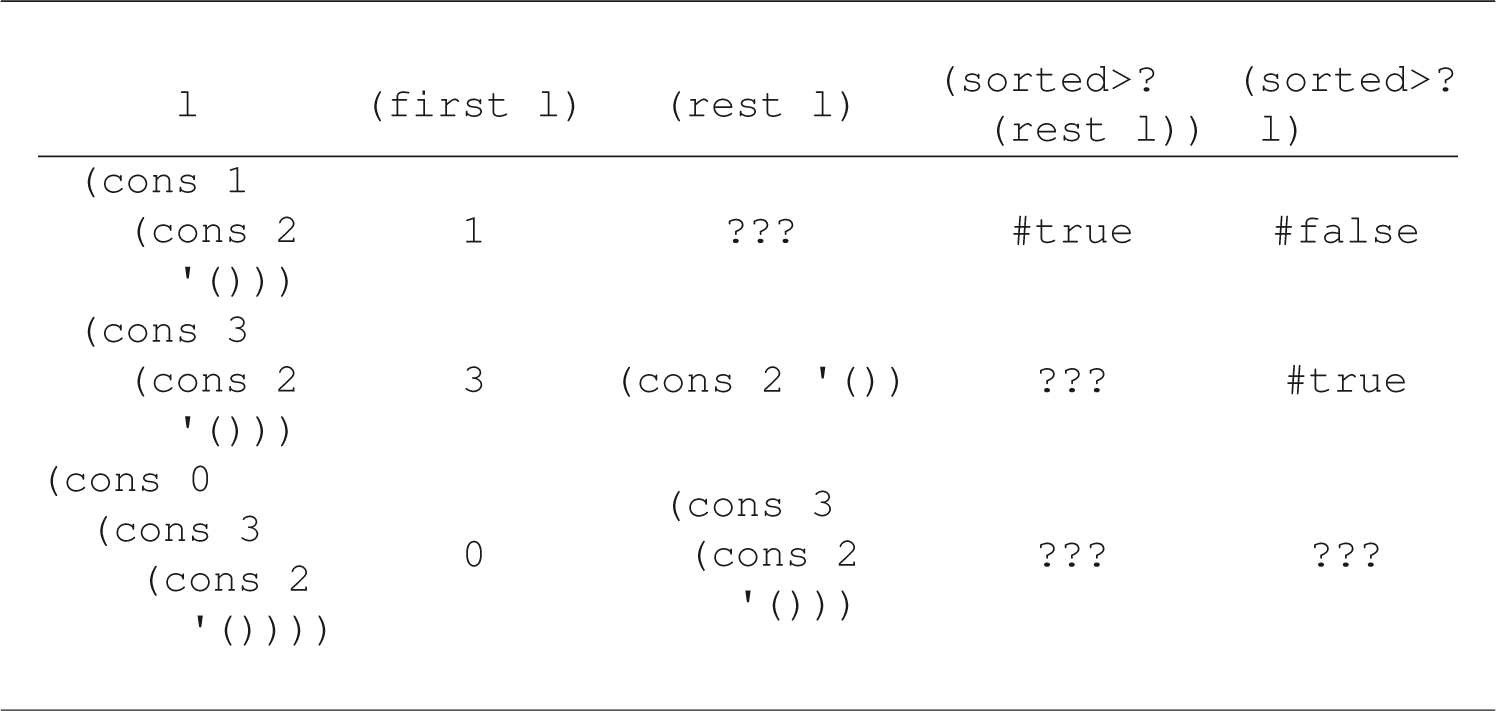
\includegraphics[width=0.8\textwidth]{images/00197.png}
  \caption{sorted>? 辅助推导表}
  \label{fig:table_for_sorted}
\end{figure}

\begin{exercise}{非空列表的 how-many}{146}
为 \code{NEList-of-temperatures} 设计专门的 \code{how-many} 函数，并确保以此重构的 \code{average} 通过所有测试。
\end{exercise}

\begin{exercise}{非空布尔列表}{147}
给出 \code{NEList-of-Booleans}（非空布尔值列表）的数据定义，并重新设计练习 140 中的 \code{all-true} 与 \code{one-true}。
\end{exercise}

\begin{exercise}{设计取舍探讨}{148}
比较本节中针对非空列表设计的函数与前一节支持空列表的函数。允许空列表的数据定义与强制非空的数据定义相比，在软件设计中孰优孰劣？为什么？
\end{exercise}

\section{自然数}
\label{sec:ch09_natural_numbers}

BSL 提供了诸如 \code{make-list} 的内置函数：它消耗一个数字 $n$ 和另一个值 $v$，产生一个包含 $n$ 个 $v$ 的列表：
\begin{replbox}
> (make-list 2 "hello")
(cons "hello" (cons "hello" '()))
> (make-list 3 #true)
(cons #true (cons #true (cons #true '())))
> (make-list 0 17)
'()
\end{replbox}

尽管它接受的是原子数据（数字），却能产生任意大小的数据！这是如何做到的？
答案在于：此处的数字并非一般的实数，而是特殊的\term{自然数}（Natural Numbers，用于计数的数）。自然数本身就是一个典型的自引用数据定义：
\begin{lstlisting}[language=BSL]
; An N（自然数）是以下之一：
; -- 0
; -- (add1 N)
; 解释：表示非负计数数字
\end{lstlisting}

第一分支表明 \code{0} 是一个自然数（表示没有被计数的对象）；第二分支表明若 $n$ 是自然数，则通过 \code{(add1 n)} 构造出的数也是自然数。在这里，\code{add1} 的角色宛如列表中的 \code{cons}，而它的配对函数 \code{sub1}（减 1）则相当于选择器！谓词 \code{zero?} 用于检查是否为基准值 \code{0}，而 \code{positive?} 用于检查是否大于 0。

基于这一自引用定义，我们来设计复制函数 \code{copier}：
\begin{lstlisting}[language=BSL]
; N String -> List-of-strings
; 创建由 n 个字符串 s 构成的列表
(check-expect (copier 0 "hello") '())
(check-expect (copier 2 "hello") (cons "hello" (cons "hello" '())))

(define (copier n s)
  (cond
    [(zero? n) '()]
    [(positive? n) (cons s (copier (sub1 n) s))]))
\end{lstlisting}

\begin{figure}[htbp]
  \centering
  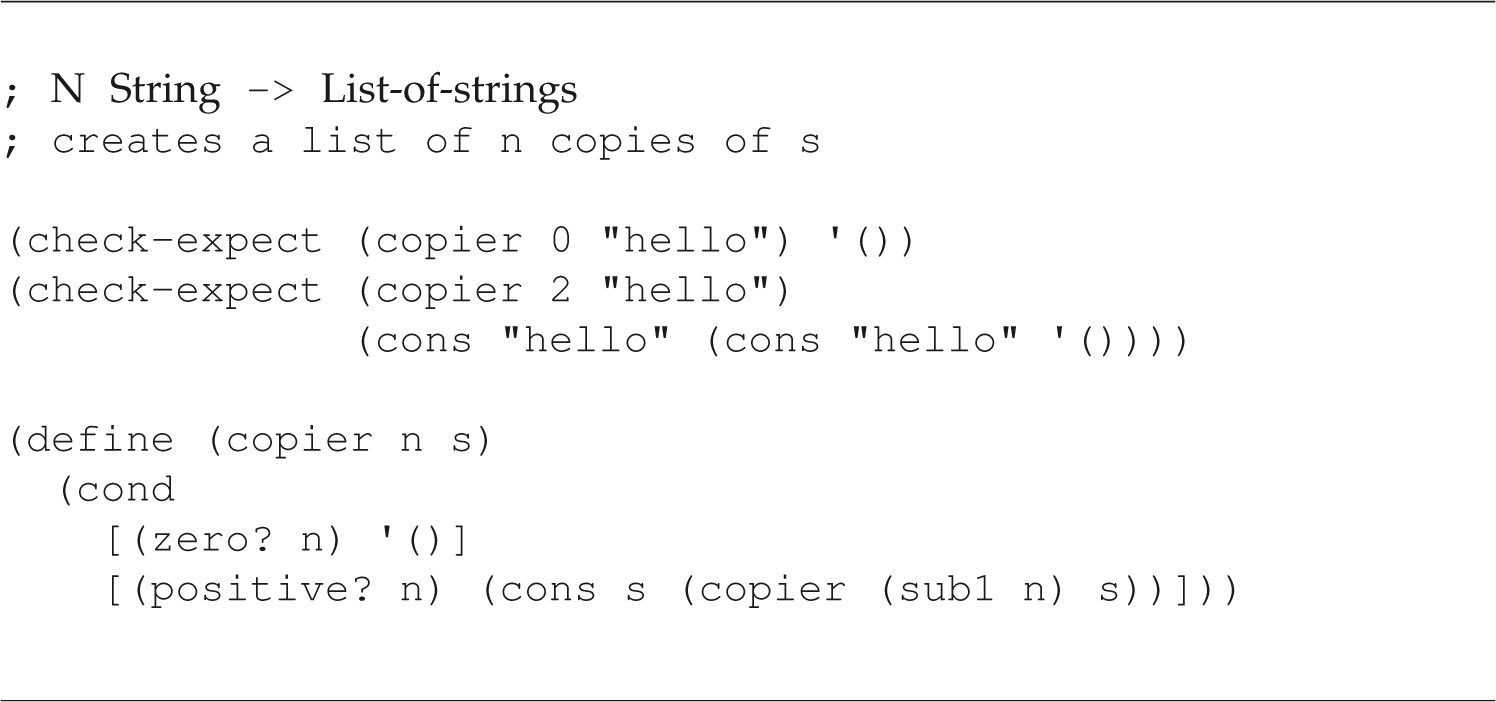
\includegraphics[width=0.85\textwidth]{images/00199.png}
  \caption{创建复制项列表}
  \label{fig:copier_definition}
\end{figure}

\begin{exercise}{类型通用性与条件分支}{149}
如果将 \code{copier} 应用于自然数和布尔值或图像，它能正常工作吗？

另外，考虑以下使用 \code{else} 的变体：
\begin{lstlisting}[language=BSL]
(define (copier.v2 n s)
  (cond
    [(zero? n) '()]
    [else (cons s (copier.v2 (sub1 n) s))]))
\end{lstlisting}
当分别对 \code{copier} 和 \code{copier.v2} 输入 \code{0.1} 和 \code{"x"} 时，二者的行为有何区别？请使用单步求值器加以验证。
\end{exercise}

\begin{exercise}{不用加号实现累加}{150}
设计函数 \code{add-to-pi}：消耗自然数 $n$，在\textbf{不使用}内置 \code{+} 运算符的前提下将其与 $\pi$ 相加。
\begin{lstlisting}[language=BSL]
; N -> Number
; 在不使用 + 的情况下计算 (+ n pi)
(check-within (add-to-pi 3) (+ 3 pi) 0.001)
(define (add-to-pi n)
  pi)
\end{lstlisting}
完成后，将其推广为通用函数 \code{add}：在不使用 \code{+} 的情况下将自然数 $n$ 与任意数 $x$ 相加。为什么测试桩代码中使用 \code{check-within}？
\end{exercise}

\begin{exercise}{不用乘号实现乘法}{151}
设计函数 \code{multiply}：消耗自然数 $n$ 与数字 $x$，在\textbf{不使用}内置 \code{*} 运算符的前提下计算两者的乘积。它与小学所学的乘法算理有何联系？
\end{exercise}

\begin{exercise}{排列图像：列与行}{152}
设计两个图像排列函数：
\begin{itemize}
  \item \code{col}：消耗自然数 $n$ 和图像 \code{img}，纵向垂直排列生成由 $n$ 个 \code{img} 组成的单列长图；
  \item \code{row}：消耗自然数 $n$ 和图像 \code{img}，横向水平排列生成由 $n$ 个 \code{img} 组成的单行长图。
\end{itemize}
\end{exercise}

\begin{exercise}{模拟教室气球袭击}{153}
利用练习 152 的函数生成一个 $8 \times 18$ 的网格矩形，每个小方格为 $10 \times 10$ 像素，放置在同等大小的空画板中作为阶梯教室。

设计函数 \code{add-balloons}：接收一个坐标落在教室范围内的 \code{Posn} 列表，产生带有红色圆点（模拟油漆水球着击点）的教室渲染图（如图~\ref{fig:random_attacks} 所示）。
\end{exercise}

\begin{figure}[htbp]
  \centering
  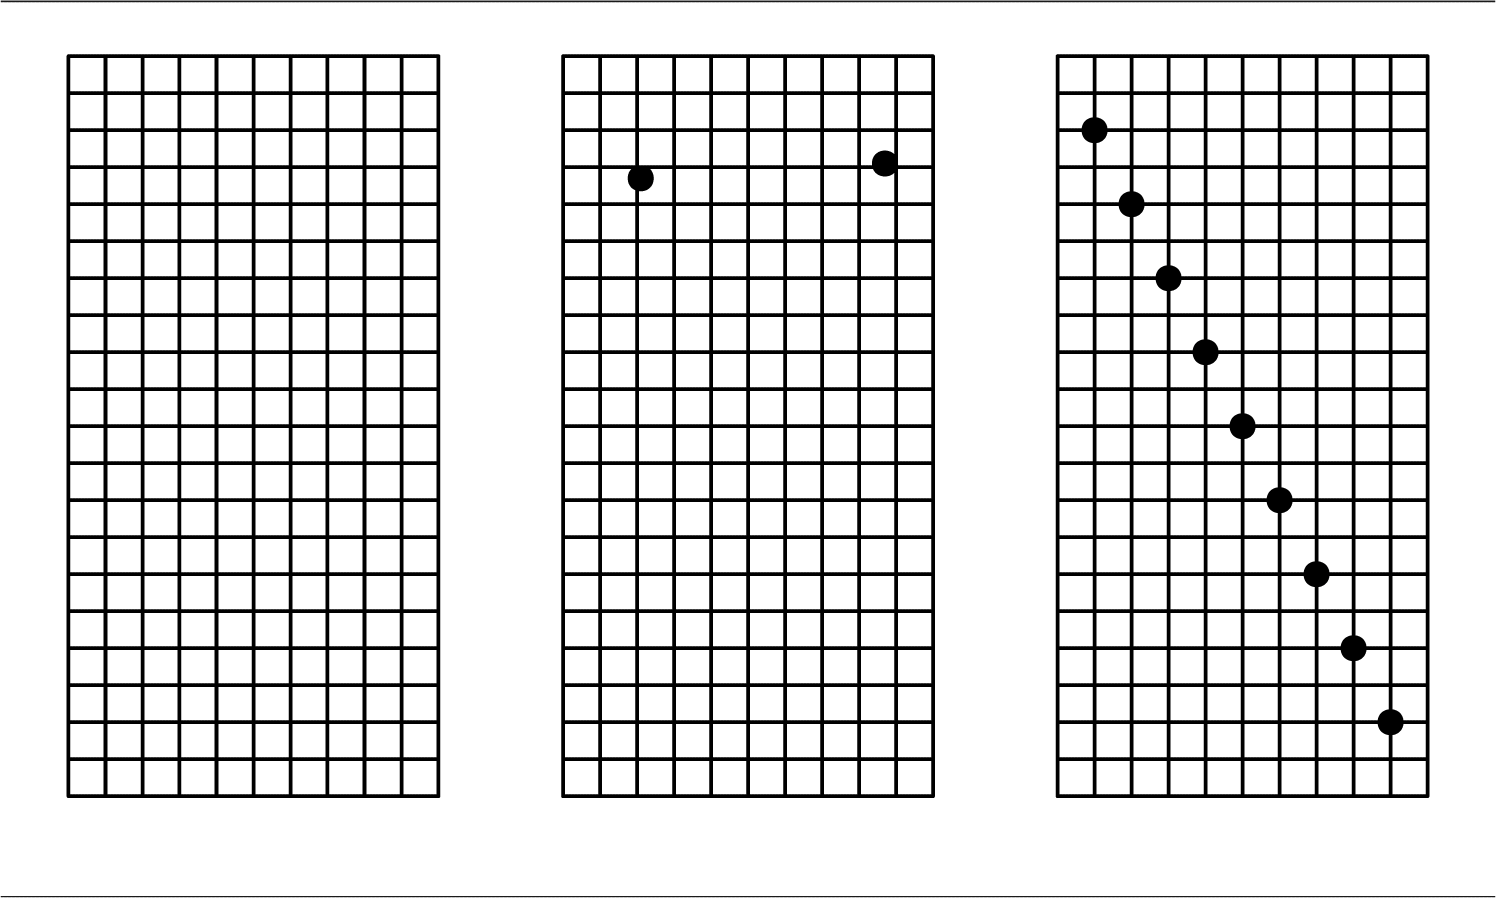
\includegraphics[width=0.85\textwidth]{images/00200.png}
  \caption{水球随机袭击模拟输出}
  \label{fig:random_attacks}
\end{figure}

\section{俄罗斯套娃}
\label{sec:ch09_russian_dolls}

维基百科将俄罗斯套娃（Russian doll）定义为“一组大小递减、层层嵌套的木制人偶”。每一层套娃都包裹着下一层更小的套娃，直到最里面是一个实心的、不再包含其他人偶的最内层人偶。

我们关注套娃的颜色属性，并用字符串来表示颜色。因此，除最内层外，每一层套娃都包含两项属性：自身的颜色、以及其内部包裹的套娃。我们用结构体来表示这种嵌套关系：
\begin{lstlisting}[language=BSL]
(define-struct layer [color doll])

; An RD（Russian doll，俄罗斯套娃）是以下之一：
; -- String
; -- (make-layer String RD)
; 解释：String 表示最内部的实心套娃的颜色；
;       (make-layer c d) 表示颜色为 c 且内部包含套娃 d 的套娃层。
\end{lstlisting}

例如，一个由黄色外层包裹着绿色中层、绿色中层包裹着红色最内层的三层套娃表示为：
\begin{lstlisting}[language=BSL]
(make-layer "yellow" (make-layer "green" "red"))
\end{lstlisting}

接下来设计函数 \code{depth} 计算套娃的总层数：
\begin{lstlisting}[language=BSL]
; RD -> Number
; 计算 an-rd 中共有多少个套娃
(check-expect (depth "red") 1)
(check-expect (depth (make-layer "yellow" (make-layer "green" "red"))) 3)

(define (depth an-rd)
  (cond
    [(string? an-rd) 1]
    [else (+ (depth (layer-doll an-rd)) 1)]))
\end{lstlisting}

\begin{exercise}{提取套娃的所有颜色}{154}
设计函数 \code{colors}：接收一个 \code{RD}，返回由逗号和空格分隔的所有外层到内层颜色的长字符串。例如上述三层套娃应返回 \code{"yellow, green, red"}。
\end{exercise}

\begin{exercise}{获取最内层颜色 inner}{155}
设计函数 \code{inner}：接收一个 \code{RD}，返回其最内层实心套娃的颜色。
\end{exercise}

\section{列表与世界}
\label{sec:ch09_lists_and_world}

有了列表之后，我们能够设计出比以往复杂得多的交互式世界程序（World Programs）。例如，在类似太空侵略者的射击游戏中，玩家不再受限于只能发射一枚导弹，而是可以任意多次按下空格键发射连续不断的弹幕。

\begin{notebox}[应用例题：弹幕射击模拟]
设计一个世界程序模拟发射子弹。每当玩家按下空格键，程序就在画布底端生成一颗子弹。所有子弹以每时钟节拍（tick）向上移动 1 像素的速度垂直上升。
\end{notebox}

首先确定常量：
\begin{lstlisting}[language=BSL]
(define HEIGHT 80)
(define WIDTH 100)
(define XSHOTS (/ WIDTH 2))

(define BACKGROUND (empty-scene WIDTH HEIGHT))
(define SHOT (triangle 3 "solid" "red"))
\end{lstlisting}

因为发射的子弹数量是动态且不确定的，所以必须使用列表来表示世界状态：
\begin{lstlisting}[language=BSL]
; A ShotWorld 是 List-of-numbers。
; 解释：列表中的每个数字代表一颗存活子弹当前的 y 坐标。
\end{lstlisting}

我们需要三个核心函数：
\begin{enumerate}
  \item \code{to-image}：将当前所有子弹绘制到背景画布上；
  \item \code{tock}：在每个时钟节拍使所有子弹的 $y$ 坐标减少 1（向上移动）；
  \item \code{keyh}：当按下空格键时，向列表中添加一颗新子弹（$y = \text{HEIGHT}$）。
\end{enumerate}

图~\ref{fig:list_based_world_program} 给出了完整的程序实现。

\begin{figure}[htbp]
  \centering
  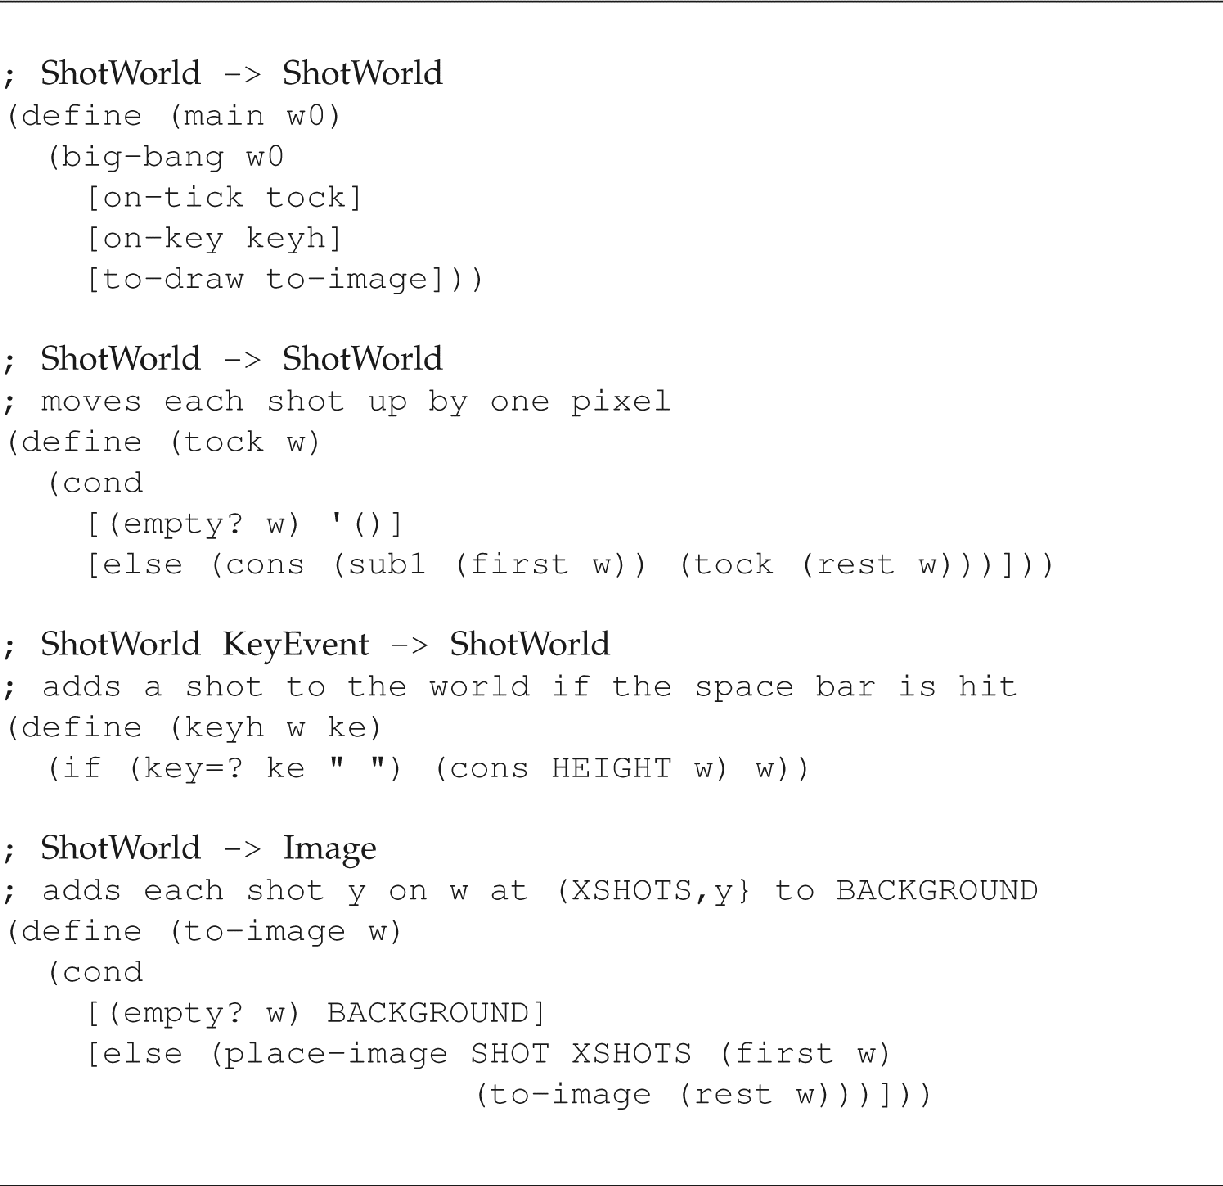
\includegraphics[width=0.9\textwidth]{images/00205.png}
  \caption{基于列表的世界程序完整代码}
  \label{fig:list_based_world_program}
\end{figure}

\begin{exercise}{运行弹幕程序}{156}
为图~\ref{fig:list_based_world_program} 中的程序编写完整的测试用例，并解释 \code{main} 函数的作用。随后在 DrRacket 中运行该程序。
\end{exercise}

\begin{exercise}{可配置常量测试}{157}
验证常量修改的灵活性：尝试修改画布高度为 220 像素、宽度为 30 像素、改变子弹颜色与发射位置等，观察程序是否只需修改单处常量即可正确响应。
\end{exercise}

\begin{exercise}{清除飞出屏幕的子弹}{158}
在图~\ref{fig:list_based_world_program} 中，飞出屏幕上边界的子弹虽然不再可见，但依然保留在列表数据中，导致列表越来越长。

设计改进版的 \code{tock} 函数：在使子弹向上移动的同时，自动剔除那些 $y < 0$ 的子弹。
\end{exercise}

\begin{exercise}{动态水球袭击世界程序}{159}
将练习 153 的方案转化为世界程序。主函数 \code{riot} 接收扔出的水球总数 $n$，以每秒 1 个的频率在随机位置投掷水球，并在窗口关闭时返回所有落点的 \code{Posn} 列表。
\end{exercise}

\section{关于列表与集合的旁注}
\label{sec:ch09_lists_and_sets}

读者可能会好奇：列表（List）与数学中的集合（Set）究竟有何异同？

从概念层面上看，集合主要用于程序设计前期的形式化讨论，而列表是编程语言中具体的一种数据结构。但更关键的区别在于处理数据时的核心关注点：
\begin{table}[htbp]
  \centering
  \caption{列表与集合的对比}
  \label{tab:lists_vs_sets}
  \begin{tabular}{lll}
    \hline
    \textbf{特征 (Property)} & \textbf{列表 (Lists)} & \textbf{集合 (Sets)} \\
    \hline
    元素归属 (Membership) & 众多特征之一 & 最核心的唯一判定标准 \\
    顺序 (Ordering) & 至关重要（有前后之分） & 无关紧要 \\
    出现次数 (\# of occurrences) & 有明确意义（允许重复） & 无关紧要（重复项不改变集合） \\
    规模大小 (Size) & 有限但可任意大 & 可以是有限的，也可以是无限的 \\
    \hline
  \end{tabular}
\end{table}

如果用有限列表来表示有限数字集合，可以采用两种策略（如图~\ref{fig:two_representations_of_sets} 所示）：
\begin{enumerate}
  \item \textbf{允许重复的列表}（\code{Son.L}）：直接使用列表，添加元素只需直接 \code{cons}，但删除元素时必须使用 \code{remove-all} 彻底清除所有重复项。
  \item \textbf{不允许重复的列表}（\code{Son.R}）：列表中的每个数字最多出现一次。添加元素时必须先检查是否已存在；而删除元素时只需使用普通的 \code{remove}。
\end{enumerate}

\begin{figure}[htbp]
  \centering
  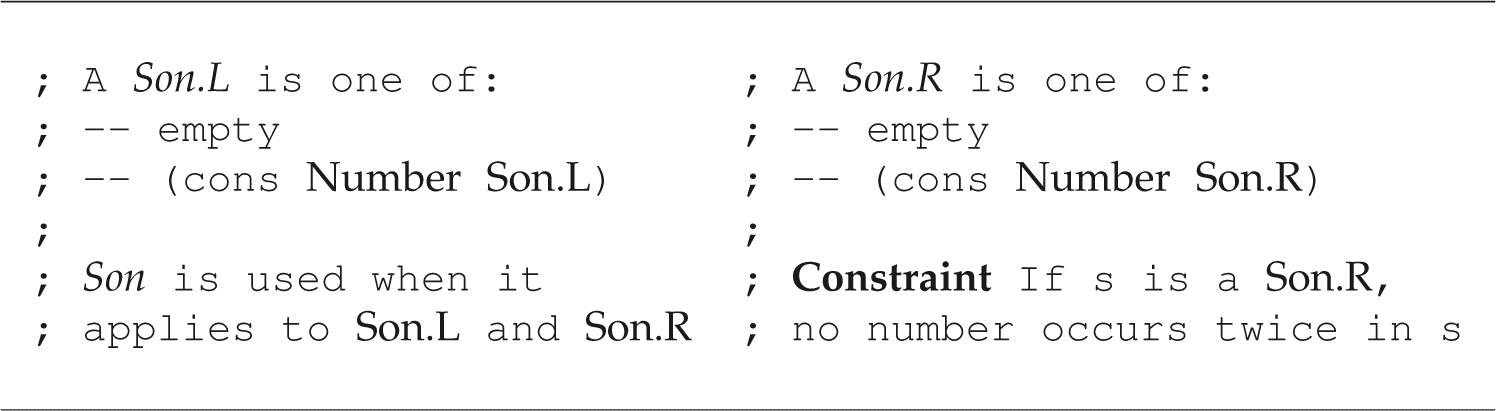
\includegraphics[width=0.85\textwidth]{images/00210.png}
  \caption{集合的两种列表数据表示形式}
  \label{fig:two_representations_of_sets}
\end{figure}

图~\ref{fig:set_functions_comparison} 对比了针对这两种集合表示形式的差集（删除元素）函数实现。

\begin{figure}[htbp]
  \centering
  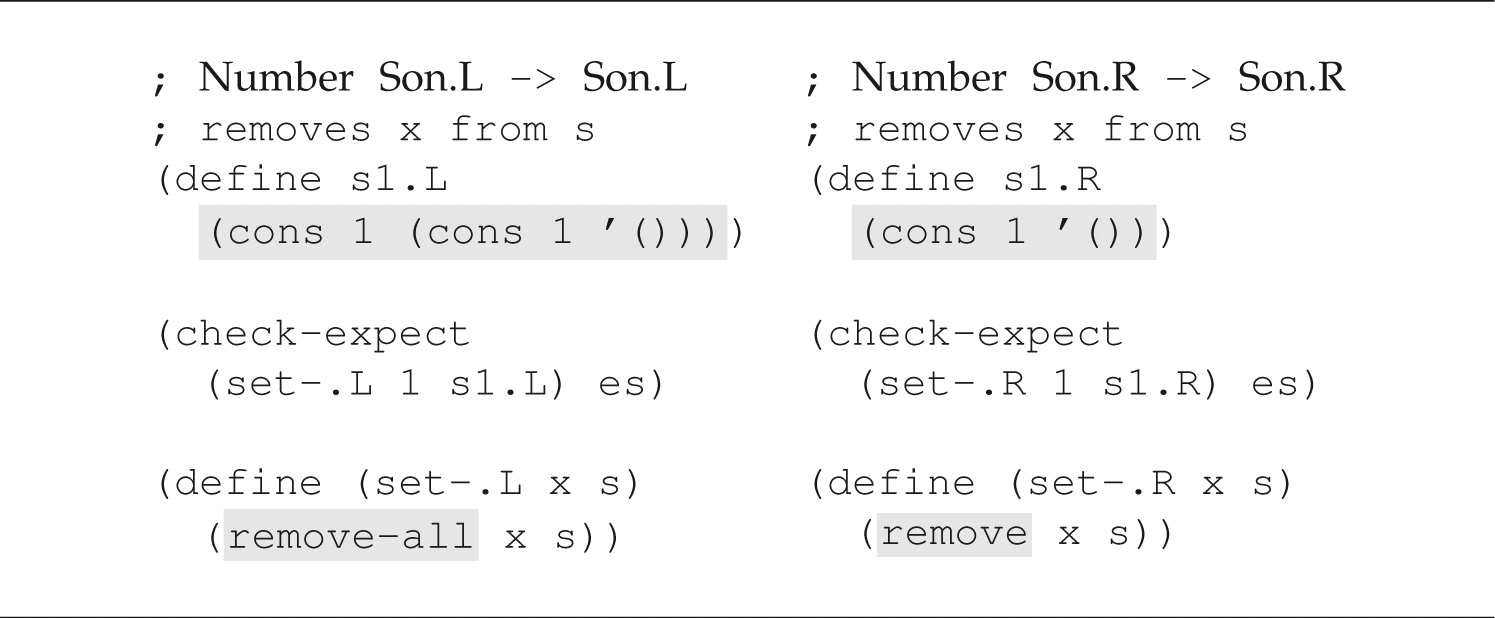
\includegraphics[width=0.85\textwidth]{images/00211.png}
  \caption{两种集合表示下的差集函数对比}
  \label{fig:set_functions_comparison}
\end{figure}

在测试集合函数时，由于集合元素的物理存储顺序并不重要，因此使用 BSL 提供的 \code{check-satisfied}（配合谓词如 \code{not-member-1?}）往往比硬编码特定列表顺序的 \code{check-expect} 更加稳健合理。

\begin{exercise}{集合添加元素函数 set+}{160}
分别针对 \code{Son.L}（允许重复）和 \code{Son.R}（不允许重复）设计添加元素函数 \code{set+.L} 与 \code{set+.R}。
\end{exercise}

% ==============================================================================
% 第 10 章：深入探讨列表 (Chapter 10: More on Lists)
% ==============================================================================

\chapter{深入探讨列表}
\label{sec:ch10_more_lists}

列表是一种功能极其多样的通用数据结构，现如今几乎所有编程语言都提供了对其的原生支持。程序员利用列表构建庞大的企业应用、人工智能系统、分布式计算平台等。本章将展示来自真实编程世界的若干核心思想，包括：产生列表的函数、在列表中嵌套结构体的数据表示法、以及将文本文件表示为多层嵌套列表。

\section{产生列表的函数}
\label{sec:ch10_functions_produce_lists}

下面是一个计算计时雇员每周薪资的简单函数：
\begin{lstlisting}[language=BSL]
; Number -> Number
; 根据工作工时 h 计算薪资
(define (wage h)
  (* 12 h))
\end{lstlisting}

该函数消耗工作工时并输出相应工资。然而，一家希望部署自动化薪酬软件的企业对这个单人函数并不感兴趣——他们需要的是一个能够批量计算公司\textbf{所有}员工薪资的程序。

我们称这个新函数为 \code{wage*}。它的任务是处理所有员工的工作工时列表，并确定每位员工应得的周薪。为简单起见，我们假设输入是一个数字列表（每个数字代表一名员工的工作小时数），期望的输出同样是一个数字列表（代表对应的每周工资）。

既然输入和输出的数据定义都是已知的数字列表，我们可以立即写出函数的头部材料：
\begin{lstlisting}[language=BSL]
; List-of-numbers -> List-of-numbers
; 根据每周工时列表计算对应的周薪列表
(define (wage* whrs)
  '())
\end{lstlisting}

接下来设计功能示例与测试用例：
\begin{lstlisting}[language=BSL]
(check-expect (wage* '()) '())
(check-expect (wage* (cons 28 '())) (cons (* 12 28) '()))
(check-expect (wage* (cons 40 (cons 28 '())))
              (cons (* 12 40) (cons (* 12 28) '())))
\end{lstlisting}

由于 \code{wage*} 消耗的数据与第 8 章中的若干函数完全相同，而函数模板仅取决于数据定义的结构，因此我们可以直接复用列表模板：
\begin{lstlisting}[language=BSL]
(define (wage* whrs)
  (cond
    [(empty? whrs) ...]
    [else (... (first whrs) ... (wage* (rest whrs)) ...)]))
\end{lstlisting}

现在进入函数体的组装环节：
\begin{itemize}
  \item 在基准情况 \code{(empty? whrs)} 下，输入为空列表，期望结果为 \code{'()}。
  \item 在自引用分支中：
    \begin{itemize}
      \item \code{(first whrs)} 给出列表中第一位员工的工时；
      \item \code{(rest whrs)} 是其余员工的工时列表；
      \item 自然递归 \code{(wage* (rest whrs))} 已经根据函数契约计算出了其余员工的周薪列表！
    \end{itemize}
\end{itemize}

既然已经拿到了除首位员工之外所有人的薪资列表，要得到全体员工的薪资列表，函数只需做两件事：
\begin{enumerate}
  \item 使用辅助函数 \code{wage} 计算第一位员工的薪资：\code{(wage (first whrs))}；
  \item 将该薪资与剩余薪资列表用 \code{cons} 拼接在一起：
\begin{lstlisting}[language=BSL]
(cons (wage (first whrs)) (wage* (rest whrs)))
\end{lstlisting}
\end{enumerate}

图~\ref{fig:wage_star_definition} 给出了完整的函数定义。

\begin{figure}[htbp]
  \centering
\begin{lstlisting}[language=BSL, basicstyle=\scriptsize\ttfamily]
; List-of-numbers -> List-of-numbers
; computes the weekly wages for all given weekly hours
(define (wage* whrs)
  (cond
    [(empty? whrs) '()]
    [else (cons (wage (first whrs)) (wage* (rest whrs)))]))

; Number -> Number
; computes the wage for h hours of work
(define (wage h)
  (* 12 h))
\end{lstlisting}
  \caption{计算所有员工薪资的 wage* 函数}
  \label{fig:wage_star_definition}
\end{figure}

\begin{exercise}{可配置的时薪常量}{161}
将上述示例转化为测试并确保全部通过。接着修改程序，使每位员工的时薪提高至 14 美元。请重构整个程序，使得将来修改全员时薪时只需修改程序中的单处常量定义，而无需更改多处代码。
\end{exercise}

\begin{exercise}{工时欺诈校验}{162}
正常情况下没有任何员工一周能工作超过 100 小时。为了保护公司免遭虚报欺诈，函数应当校验输入列表中没有任何一项超过 100。一旦发现超过 100 的数值，函数应立即报错。请修改图~\ref{fig:wage_star_definition} 中的函数以实现这一基础现实核查。
\end{exercise}

\begin{exercise}{华氏度转摄氏度列表 convertFC}{163}
设计函数 \code{convertFC}：将测量得到的华氏度温度列表转换为对应的摄氏度列表。
\end{exercise}

\begin{exercise}{货币汇率转换 convert-euro}{164}
设计函数 \code{convert-euro}：将美元金额列表转换为欧元金额列表。

接着将其推广为函数 \code{convert-euro*}：消耗一个指定的汇率数值与美元列表，完成相应的欧元列表转换。
\end{exercise}

\begin{exercise}{玩具名称替换 subst-robot}{165}
设计函数 \code{subst-robot}：消耗玩具描述字符串列表，将其中的所有 \code{"robot"} 替换为 \code{"r2d2"}，其余玩具描述保持不变。

接着将其推广为通用替换函数 \code{substitute}：消耗两个字符串 \code{new} 和 \code{old} 以及一个字符串列表，将列表中所有的 \code{old} 全部替换为 \code{new}。
\end{exercise}

\section{列表中的结构体}
\label{sec:ch10_structures_in_lists}

仅用一个工时数字来表示一周的工作记录在实际应用中是远远不够的，因为打印工资单还需要员工姓名，且员工之间的时薪往往各不相同。幸运的是，列表不仅能存放原子数据，还能存放结构体！

我们定义工作记录结构体 \code{work}：
\begin{lstlisting}[language=BSL]
(define-struct work [employee rate hours])
; A Work 是一个结构体：
;   (make-work String Number Number)
; 解释：(make-work n r h) 将员工姓名 n、时薪 r 与工时 h 组合在一起
\end{lstlisting}

进而定义工作记录的列表：
\begin{lstlisting}[language=BSL]
; Low (List-of-works) 是以下之一：
; -- '()
; -- (cons Work Low)
; 解释：表示若干员工的工作记录列表
\end{lstlisting}

现在我们来重新设计薪资计算函数，命名为 \code{wage*.v2}：
\begin{lstlisting}[language=BSL]
; Low -> List-of-numbers
; 根据工作记录列表计算对应的周薪列表
(define (wage*.v2 an-low)
  '())
\end{lstlisting}

\begin{notebox}[设计原则：分解模板与辅助函数]
当一个数据定义（如 \code{Low}）引用了另一个复杂数据定义（如 \code{Work}）时，最佳策略是\textbf{分别构建独立的模板与函数}，而不是将结构体的所有选择器强行堆积在列表的单个分支中。将任务合理切分给专门处理 \code{Work} 的辅助函数，能保持代码清晰、易维护且易测试。
\end{notebox}

图~\ref{fig:computing_wages_from_work_records} 展示了切分后的完整设计：由 \code{wage*.v2} 负责遍历列表，调用辅助函数 \code{wage.v2} 计算单个记录的周薪。

\begin{figure}[htbp]
  \centering
\begin{lstlisting}[language=BSL, basicstyle=\scriptsize\ttfamily]
; Low -> List-of-numbers
; computes the weekly wages for all weekly work records

(check-expect
  (wage*.v2 (cons (make-work "Robby" 11.95 39) '()))
  (cons (* 11.95 39) '()))

(define (wage*.v2 an-low)
  (cond
    [(empty? an-low) '()]
    [(cons? an-low) (cons (wage.v2 (first an-low))
                          (wage*.v2 (rest an-low)))]))

; Work -> Number
; computes the wage for the given work record w
(define (wage.v2 w)
  (* (work-rate w) (work-hours w)))
\end{lstlisting}
  \caption{从工作记录计算周薪的完整程序}
  \label{fig:computing_wages_from_work_records}
\end{figure}

\begin{exercise}{迭代细化：产生工资支票列表}{166}
\code{wage*.v2} 消耗工作记录列表并产生数字列表。当然，函数也可以产生结构体列表。

为工资支票（paycheck）开发数据表示，假设支票包含员工姓名与实发薪资金额两项信息。接着设计函数 \code{wage*.v3}：消耗 \code{Low} 并产生对应的支票列表。

在真实世界中，工资支票还包含员工工号（employee number）。请为包含工号的员工信息开发数据表示，相应更新工作记录与支票的数据定义，并设计 \code{wage*.v4}。
\end{exercise}

\begin{exercise}{坐标列表求和 sum}{167}
设计函数 \code{sum}：接收一个 \code{Posn} 列表，计算其中所有点 $x$ 坐标的总和。
\end{exercise}

\begin{exercise}{坐标平移 translate}{168}
设计函数 \code{translate}：消耗并产生 \code{Posn} 列表。对输入中的每个 \code{(make-posn x y)}，输出列表中对应项为 \code{(make-posn x (+ y 1))}。
\end{exercise}

\begin{exercise}{合法坐标筛选 legal}{169}
设计函数 \code{legal}：消耗并产生 \code{Posn} 列表，筛选出所有 $x$ 坐标落在 $[0, 100]$ 且 $y$ 坐标落在 $[0, 200]$ 范围内的合法点。
\end{exercise}

\begin{exercise}{电话区号批量更新 replace}{170}
给定电话号码的数据定义：
\begin{lstlisting}[language=BSL]
(define-struct phone [area switch four])
; A Phone 是一个结构体：
;   (make-phone Three Three Four)
; A Three 是 [100, 999] 之间的 Number。
; A Four 是 [1000, 9999] 之间的 Number。
\end{lstlisting}
设计函数 \code{replace}：消耗并产生 \code{Phone} 列表，将其中的所有 713 区号替换为 281。
\end{exercise}

\section{列表嵌套列表与文件}
\label{sec:ch10_lists_in_lists_files}

在计算机系统中，文本文件不仅仅是一长串纯文本字符，它们通常具有行与单词、表格行列与单元格等多层组织结构。在 BSL 中，通过 \code{2htdp/batch-io} 教学库，我们能够将文本文件解析为多层结构：
\begin{itemize}
  \item \textbf{按行读取}（\code{read-lines}）：生成字符串列表，每行表示为一个字符串；
  \item \textbf{按词读取}（\code{read-words}）：生成单词字符串列表；
  \item \textbf{按行与词读取}（\code{read-words/line}）：生成\term{由单词列表构成的行列表}，即\textbf{列表嵌套列表}（List of lists of strings, LLS）！
\end{itemize}

图~\ref{fig:reading_files} 总结了 \code{2htdp/batch-io} 中用于读取文件的常用函数。

\begin{figure}[htbp]
  \centering
\begin{lstlisting}[language=BSL, basicstyle=\scriptsize\ttfamily]
; String -> String
; produces the content of file f as a string
(define (read-file f) ...)

; String -> List-of-string
; produces the content of file f as a list of strings,
; one per line
(define (read-lines f) ...)

; String -> List-of-string
; produces the content of file f as a list of strings,
; one per word
(define (read-words f) ...)

; String -> List-of-list-of-string
; produces the content of file f as a list of list of
; strings, one list per line and one string per word
(define (read-words/line f) ...)

; The above functions consume the name of a file as a String
; argument. If the specified file does not exist in the
; same folder as the program, they signal an error.
\end{lstlisting}
  \caption{文件读取函数概览}
  \label{fig:reading_files}
\end{figure}

\begin{exercise}{表示 Piet Hein 的诗歌 TTT}{171}
给出 \code{List-of-strings} 与 \code{List-of-list-of-strings}（LLS）的数据定义，并使用 \code{read-lines}、\code{read-words} 与 \code{read-words/line} 验证皮特·海恩（Piet Hein）的短诗在不同表示下的数据形态。
\end{exercise}

以统计文本文件每行字数的任务为例，我们定义函数 \code{words-on-line}：
\begin{lstlisting}[language=BSL]
; LLS -> List-of-numbers
; 计算每行中包含的单词数量
(define (words-on-line lls)
  (cond
    [(empty? lls) '()]
    [else (cons (length (first lls))
                (words-on-line (rest lls)))]))
\end{lstlisting}

图~\ref{fig:counting_words_on_line} 展示了该函数的设计与测试。借助这一基础，我们只需将其与内置的 \code{read-words/line} 进行组合，便能一行代码写出实用的文件统计工具：
\begin{lstlisting}[language=BSL]
; String -> List-of-numbers
; 统计指定文本文件各行的单词数
(define (file-statistic file-name)
  (words-on-line (read-words/line file-name)))
\end{lstlisting}

\begin{figure}[htbp]
  \centering
\begin{lstlisting}[language=BSL, basicstyle=\scriptsize\ttfamily]
; An LLS is one of:
; -- '()
; -- (cons Los LLS)
; interpretation a list of lines, each is a list of Strings

(define line0 (cons "hello" (cons "world" '())))
(define line1 '())

(define lls0 '())
(define lls1 (cons line0 (cons line1 '())))

; LLS -> List-of-numbers
; determines the number of words on each line

(check-expect (words-on-line lls0) '())
(check-expect (words-on-line lls1) (cons 2 (cons 0 '())))

(define (words-on-line lls)
  (cond
    [(empty? lls) '()]
    [else (cons (length (first lls))
                (words-on-line (rest lls)))]))
\end{lstlisting}
  \caption{统计每行字数的函数设计}
  \label{fig:counting_words_on_line}
\end{figure}

\begin{exercise}{还原文件内容 collapse}{172}
设计函数 \code{collapse}：将行列表还原为一个完整的长字符串，单词间以空格 \code{" "} 分隔，行间以换行符 \code{"\textbackslash n"} 分隔。
\end{exercise}

\begin{exercise}{过滤冠词程序}{173}
设计一个程序剔除文本文件中的所有英文冠词（\code{"a"}、\code{"an"}、\code{"the"}）。程序读取指定文件，过滤冠词后输出至名为 \code{"no-articles-" + filename} 的新文件中。
\end{exercise}

\begin{exercise}{文本文件数字编码}{174}
设计程序对文本文件进行数字编码，将单词中的每个字符编码为 0 到 256 之间的 3 位数字字符串（如图~\ref{fig:encoding_strings} 所示）。
\end{exercise}

\begin{figure}[htbp]
  \centering
\begin{lstlisting}[language=BSL, basicstyle=\scriptsize\ttfamily]
; 1String -> String
; converts the given 1String to a 3-letter numeric String

(check-expect (encode-letter "z") (code1 "z"))
(check-expect (encode-letter "\t")
              (string-append "00" (code1 "\t")))
(check-expect (encode-letter "a")
              (string-append "0" (code1 "a")))

(define (encode-letter s)
  (cond
    [(>= (string->int s) 100) (code1 s)]
    [(< (string->int s) 10)
     (string-append "00" (code1 s))]
    [(< (string->int s) 100)
     (string-append "0" (code1 s))]))

; 1String -> String
; converts the given 1String into a String

(check-expect (code1 "z") "122")

(define (code1 c)
  (number->string (string->int c)))
\end{lstlisting}
  \caption{单字符编码函数}
  \label{fig:encoding_strings}
\end{figure}

\begin{exercise}{模拟 Unix wc 命令}{175}
编写 BSL 程序模拟 Unix 系统的 \code{wc} 命令行工具：统计给定文本文件中的单字符数（1Strings）、单词数与总行数。
\end{exercise}

\begin{exercise}{矩阵表示与转置 transpose}{176}
将矩阵定义为行的列表（每行又是数字列表）：
\begin{lstlisting}[language=BSL]
; A Matrix 是以下之一：
; -- (cons Row '())
; -- (cons Row Matrix)
; 约束：矩阵中所有行的长度必须相等

; A Row 是以下之一：
; -- '()
; -- (cons Number Row)
\end{lstlisting}
图~\ref{fig:transpose_matrix} 展示了矩阵转置函数 \code{transpose} 的骨架，它依赖辅助函数 \code{first*}（提取首列）与 \code{rest*}（剔除首列）。请设计这两个辅助函数并补全测试。
\end{exercise}

\begin{figure}[htbp]
  \centering
\begin{lstlisting}[language=BSL, basicstyle=\scriptsize\ttfamily]
; Matrix -> Matrix
; transposes the given matrix along the diagonal

(define wor1 (cons 11 (cons 21 '())))
(define wor2 (cons 12 (cons 22 '())))
(define tam1 (cons wor1 (cons wor2 '())))

(check-expect (transpose mat1) tam1)

(define (transpose lln)
  (cond
    [(empty? (first lln)) '()]
    [else (cons (first* lln) (transpose (rest* lln)))]))
\end{lstlisting}
  \caption{矩阵转置函数}
  \label{fig:transpose_matrix}
\end{figure}

\section{重温图形文本编辑器}
\label{sec:ch10_editor_revisited}

在第 5.10 节中，我们曾通过结构体设计过单行文本编辑器。现在，借助列表的力量，我们可以给出一种在算法效率和概念上都极其优雅的数据表示：
\begin{lstlisting}[language=BSL]
(define-struct editor [pre post])
; An Editor 是一个结构体：
;   (make-editor Lo1S Lo1S)
; An Lo1S (List of 1Strings) 是以下之一：
; -- '()
; -- (cons 1String Lo1S)
\end{lstlisting}

\begin{notebox}[关键设计决策：逆序存储光标左侧字符]
我们令 \code{pre} 字段以\textbf{逆序}（reverse order）存储光标左侧的字符，而 \code{post} 字段以\textbf{正序}存储光标右侧的字符！
例如，当文本为 \code{"all|good"}（光标位于中间）时：
\begin{lstlisting}[language=BSL]
(make-editor (cons "l" (cons "l" (cons "a" '())))
             (cons "g" (cons "o" (cons "o" (cons "d" '())))))
\end{lstlisting}
这种表示的威力在于：\textbf{所有在光标附近的编辑操作（打字、退格、左右移动）都只发生在列表的最前端（head）}！在列表前端插入或删除只需一步 \code{cons} 或 \code{first/rest}，其时间复杂度为 $O(1)$，效率极高！
\end{notebox}

为此，我们需要列表逆序函数 \code{rev}（或 BSL 内置的 \code{reverse}）：
\begin{figure}[htbp]
  \centering
  \begin{stepperbox}[unbreakable]
    \centering
    \scriptsize
    \setlength{\tabcolsep}{3pt}
    \begin{tabular}{lllll}
      \toprule
      \texttt{l} &
      \begin{tabular}[t]{@{}l@{}}\texttt{(first}\\\texttt{~~l)}\end{tabular} &
      \begin{tabular}[t]{@{}l@{}}\texttt{(rest}\\\texttt{~~l)}\end{tabular} &
      \begin{tabular}[t]{@{}l@{}}\texttt{(rev}\\\texttt{~~(rest l))}\end{tabular} &
      \texttt{(rev l)} \\
      \midrule
      \begin{tabular}[t]{@{}l@{}}\texttt{(cons "a"}\\\texttt{~~'())}\end{tabular} &
      \texttt{"a"} & \texttt{'()} & \texttt{'()} &
      \begin{tabular}[t]{@{}l@{}}\texttt{(cons "a"}\\\texttt{~~'())}\end{tabular} \\
      \addlinespace[3pt]
      \begin{tabular}[t]{@{}l@{}}\texttt{(cons "a"}\\\texttt{~~(cons "b"}\\\texttt{~~~~(cons "c"}\\\texttt{~~~~~~'())))}\end{tabular} &
      \texttt{"a"} &
      \begin{tabular}[t]{@{}l@{}}\texttt{(cons "b"}\\\texttt{~~(cons "c"}\\\texttt{~~~~'()))}\end{tabular} &
      \begin{tabular}[t]{@{}l@{}}\texttt{(cons "c"}\\\texttt{~~(cons "b"}\\\texttt{~~~~'()))}\end{tabular} &
      \begin{tabular}[t]{@{}l@{}}\texttt{(cons "c"}\\\texttt{~~(cons "b"}\\\texttt{~~~~(cons "a"}\\\texttt{~~~~~~'())))}\end{tabular} \\
      \bottomrule
    \end{tabular}
  \end{stepperbox}
  \caption{rev 函数的设计推导表}
  \label{fig:tabulating_rev}
\end{figure}

\begin{exercise}{构造编辑器状态 create-editor}{177}
设计函数 \code{create-editor}：接收两个字符串（分别代表光标左侧和右侧的文本），构造出一个符合上述逆序约定的 \code{Editor}。
\end{exercise}

键盘事件处理函数 \code{editor-kh} 根据按键类型分发任务：
\begin{lstlisting}[language=BSL]
(define (editor-kh ed ke)
  (cond
    [(key=? ke "left") (editor-lft ed)]
    [(key=? ke "right") (editor-rgt ed)]
    [(key=? ke "\b") (editor-del ed)]
    [(key=? ke "\t") ed]
    [(key=? ke "\r") ed]
    [(= (string-length ke) 1) (editor-ins ed ke)]
    [else ed]))
\end{lstlisting}

\begin{exercise}{按键优先级判定}{178}
解释为什么在 \code{editor-kh} 中必须在检查单字符之前优先处理 \code{"\textbackslash t"} 与 \code{"\textbackslash r"}？
\end{exercise}

插入字符函数 \code{editor-ins} 极为简洁明快：
\begin{lstlisting}[language=BSL]
; Editor 1String -> Editor
; 在光标所在处插入单字符 k
(define (editor-ins ed k)
  (make-editor (cons k (editor-pre ed))
               (editor-post ed)))
\end{lstlisting}

\begin{exercise}{光标移动与删除}{179}
设计以下三个编辑操作函数：
\begin{itemize}
  \item \code{editor-lft}：光标向左移动一个字符（将 \code{pre} 的首元素转移到 \code{post} 的前端）；
  \item \code{editor-rgt}：光标向右移动一个字符（将 \code{post} 的首元素转移到 \code{pre} 的前端）；
  \item \code{editor-del}：退格删除光标左侧的一个字符（丢弃 \code{pre} 的首元素）。
\end{itemize}
\end{exercise}

\begin{exercise}{文本渲染函数 editor-text}{180}
在不使用 BSL 内置 \code{implode} 的前提下，设计将 \code{Lo1S} 转换为文本图像的 \code{editor-text} 函数。
\end{exercise}

% ==============================================================================
% 第 11 章：组合设计 (Chapter 11: Design by Composition)
% ==============================================================================

\chapter{组合设计}
\label{sec:ch11_design_by_composition}

至此，你已经深刻体会到现实中的程序往往是复杂的智力产物，它们的实现依赖于多个相互协作的函数。只有当软件设计者深刻理解\textbf{何时需要划分多个函数}以及\textbf{如何将这些函数有机组合为一个完整程序}时，协作才能顺畅进行。

在之前的章节中，你已经多次遇到设计相关联函数的需求：有时是因为问题描述中隐含了多个不同维度的子任务，每个任务最适合由一个独立函数完成；有时则是因为一个数据定义引用了另一个数据定义，此时处理前者的函数理应调用处理后者的辅助函数。

本章将介绍若干需要组合多个函数的典型编程场景，并提供关于拆分与组合函数的指导准则。为了让代码书写更简练，我们首先介绍初学学生语言关于列表的简写扩展。

\section{list 简写函数}
\label{sec:ch11_the_list_function}

写了这么多次连续嵌套的 \code{cons} 之后，你可能已经对频繁书写 \code{(cons ... (cons ... '()))} 感到厌烦，特别是在处理长列表时。幸运的是，DrRacket 提供了包含列表简写功能的“带有列表简写的初学学生语言”（BSL+）。

\begin{notebox}[切换教学语言]
现在是升级的时候了！请在 DrRacket 的“Language（语言）”菜单中选择“Beginning Student with List Abbreviations（带有列表简写的初学学生语言）”。
\end{notebox}

最核心的革新在于引入了 \code{list} 函数。它接受任意数量的参数并构造出一个列表。理解 \code{list} 最简单的方法是将其视为宏简写：任何形如下式的表达式
\begin{lstlisting}[language=BSL]
(list exp-1 ... exp-n)
\end{lstlisting}
等价于 $n$ 次嵌套的 \code{cons} 表达式：
\begin{lstlisting}[language=BSL]
(cons exp-1 (cons ... (cons exp-n '())))
\end{lstlisting}
请注意，\code{'()} 并不是列表的元素之一，而是充当列表末尾的终止哨兵。

当然，\code{list} 的参数不仅可以是常量值，也可以是待求值的子表达式：
\begin{replbox}
> (list (+ 0 1) (+ 1 1))
(list 1 2)
> (list (/ 1 0) (+ 1 1))
/: division by zero
\end{replbox}
在构建列表之前，所有参数表达式都会被首先求值。如果其中任何一个表达式报错，列表将根本不会被构造出来。简而言之，\code{list} 的求值行为与任何接收任意参数的标准操作一致。

使用 \code{list} 极大地简化了多层嵌套列表或包含结构体的列表的书写：
\begin{lstlisting}[language=BSL]
(list 0 1 2 3 4 5 6 7 8 9)
\end{lstlisting}
只需一次 \code{list} 调用，而传统写法需要 10 次 \code{cons} 和一个 \code{'()}。

\begin{exercise}{使用 list 重写列表}{181}
使用 \code{list} 构造等价于下列各式的列表：
\begin{enumerate}
  \item \code{(cons "a" (cons "b" (cons "c" (cons "d" '()))))}
  \item \code{(cons (cons 1 (cons 2 '())) '())}
  \item \code{(cons "a" (cons (cons 1 '()) (cons \#false '())))}
  \item \code{(cons (cons "a" (cons 2 '())) (cons "hello" '()))}
\end{enumerate}
使用 \code{check-expect} 编写测试，确保你的简写版本与展开版本求值结果完全一致。
\end{exercise}

\begin{exercise}{展开 list 简写为 cons}{182}
使用基础的 \code{cons} 和 \code{'()} 还原下列列表：
\begin{enumerate}
  \item \code{(list 0 1 2 3 4 5)}
  \item \code{(list (list "he" 0) (list "it" 1) (list "lui" 14))}
  \item \code{(list 1 (list 1 2) (list 1 2 3))}
\end{enumerate}
\end{exercise}

\begin{exercise}{混合构造展开}{183}
将下列混用 \code{cons} 与 \code{list} 的表达式分别重构为：仅使用 \code{cons} 的版本，以及尽可能仅使用 \code{list} 的版本：
\begin{enumerate}
  \item \code{(cons "a" (list 0 \#false))}
  \item \code{(list (cons 1 (cons 13 '())))}
  \item \code{(cons (list 1 (list 13 '())) '())}
  \item \code{(list '() '() (cons 1 '()))}
  \item \code{(cons "a" (cons (list 1) (list \#false '())))}
\end{enumerate}
\end{exercise}

\begin{exercise}{表达式求值预测}{184}
在不运行 DrRacket 的情况下，推导下列表达式的值，并在 DrRacket 中通过 \code{check-expect} 加以验证：
\begin{enumerate}
  \item \code{(list (string=? "a" "b") \#false)}
  \item \code{(list (+ 10 20) (* 10 20) (/ 10 20))}
  \item \code{(list "dana" "jane" "mary" "laura")}
\end{enumerate}
\end{exercise}

\begin{exercise}{探索更多选择器}{185}
BSL+ 在 \code{first} 和 \code{rest} 之外还提供了许多便利的选择器。推导下式的值：
\begin{enumerate}
  \item \code{(first (list 1 2 3))}
  \item \code{(rest (list 1 2 3))}
  \item \code{(second (list 1 2 3))}
\end{enumerate}
查阅 DrRacket 文档，确认是否内置了 \code{third}、\code{fourth} 等更高阶的位置选择器。
\end{exercise}

\section{组合函数}
\label{sec:ch11_composing_functions}

回顾之前的设计指导准则：
\begin{itemize}
  \item \textbf{单一任务原则}：一个函数只负责一个明确的任务。当问题涉及不同数量间的依赖时，为其构建独立的辅助函数。
  \item \textbf{单一模板原则}：一个数据定义对应一个函数模板。当一个数据定义指向另一个数据定义时，为主函数构建处理被指向数据的辅助函数。
\end{itemize}

在将模板实例化为具体函数体（即组装子表达式的计算结果）时，以下四种情境强烈提示你需要引入\term{辅助函数}：
\begin{enumerate}
  \item \textbf{特定领域知识}：若值的组合涉及专业领域规则（如图像图形渲染、会计税收计算、音乐、几何学或物理学等），应将其抽离为辅助函数。
  \item \textbf{复杂的条件分析}：若值的组合需要对已有值进行繁琐的多情况分支判定（如正数、零、负数的不同计算），应将该 \code{cond} 逻辑封装为独立的辅助函数。
  \item \textbf{处理自引用数据元素}：若值的组合必须遍历处理另一个任意大小的数据（列表、自然数等），必须为此设计一个递归辅助函数。
  \item \textbf{泛化与抽象}：若直接求解原问题遇到阻碍，先设计一个求解\textbf{更一般化问题}的函数，再将原问题作为该通用特例予以调用！
\end{enumerate}

\begin{notebox}[愿望清单 (Wish List)]
在多函数协作开发中，核心在于维护一张\term{愿望清单}（Wish List）：记录所有为了完成当前程序而“期望存在”的辅助函数头部材料（签名、目的说明与桩定义）。
\begin{itemize}
  \item 只要愿望清单上的函数有桩定义，主程序就能直接进行局部测试；
  \item 当愿望清单清空时，整个软件的所有函数均已完工并通过测试！
\end{itemize}
在向愿望清单添加新项前，务必先检查语言标准库中是否已有现成函数。
\end{notebox}

\section{递归辅助函数}
\label{sec:ch11_auxiliary_functions_recur}

排序是计算机科学中最基础也最核心的问题之一。本节我们将通过解决一个经典的排序问题来展示递归辅助函数的设计：

\begin{notebox}[例题：实数列表降序排序]
设计函数 \code{sort>}，接收一个数字列表并输出一个按降序排列（从大到小）的新列表。
\end{notebox}

我们首先给出签名、目的说明与桩函数：
\begin{lstlisting}[language=BSL]
; List-of-numbers -> List-of-numbers
; 将 alon 重排为按降序排列的列表
(check-expect (sort> '()) '())
(check-expect (sort> (list 12 20 -5)) (list 20 12 -5))
(check-expect (sort> (list 3 2 1)) (list 3 2 1))
(check-expect (sort> (list 1 2 3)) (list 3 2 1))

(define (sort> alon)
  '())
\end{lstlisting}

根据列表模板推导：
\begin{lstlisting}[language=BSL]
(define (sort> alon)
  (cond
    [(empty? alon) '()]
    [else (... (first alon) ... (sort> (rest alon)) ...)]))
\end{lstlisting}

考察自引用分支：
\begin{itemize}
  \item \code{(first alon)} 提取首个数字（例如 \code{12}）；
  \item 自然递归 \code{(sort> (rest alon))} 已经正确地将剩余列表排好序（例如得到 \code{(list 20 -5)}）！
\end{itemize}
现在的关键任务是：\textbf{如何将首元素 \code{12} 插入到已经排好序的列表 \code{(list 20 -5)} 的正确位置上？}

在有序列表中插入一个数字需要遍历该列表以找到合适的插入位置。由于列表是任意大小的数据，根据准则 3，这必须委托给一个独立的辅助函数：
\begin{lstlisting}[language=BSL]
; Number List-of-numbers -> List-of-numbers
; 将数字 n 插入到已经按降序排列的列表 alon 中的合适位置
(define (insert n alon)
  alon)
\end{lstlisting}

有了这个愿望清单中的 \code{insert}，主函数 \code{sort>} 即可立刻落笔成型：
\begin{lstlisting}[language=BSL]
(define (sort> alon)
  (cond
    [(empty? alon) '()]
    [else (insert (first alon) (sort> (rest alon)))]))
\end{lstlisting}

接下来设计 \code{insert}：
\begin{lstlisting}[language=BSL]
(check-expect (insert 5 '()) (list 5))
(check-expect (insert 5 (list 6)) (list 6 5))
(check-expect (insert 5 (list 4)) (list 5 4))
(check-expect (insert 12 (list 20 -5)) (list 20 12 -5))
\end{lstlisting}

在 \code{insert} 中，若列表为空，则返回 \code{(list n)}；若列表非空，且 $n \ge \text{首元素}$，由于后续元素更小，故直接 \code{(cons n alon)}；否则，首元素保留在最前，将 $n$ 递归插入到剩余部分中：\code{(cons (first alon) (insert n (rest alon)))}。

图~\ref{fig:sorting_lists_of_numbers} 展示了完整的\term{插入排序}（Insertion Sort）程序。

\begin{figure}[htbp]
  \centering
  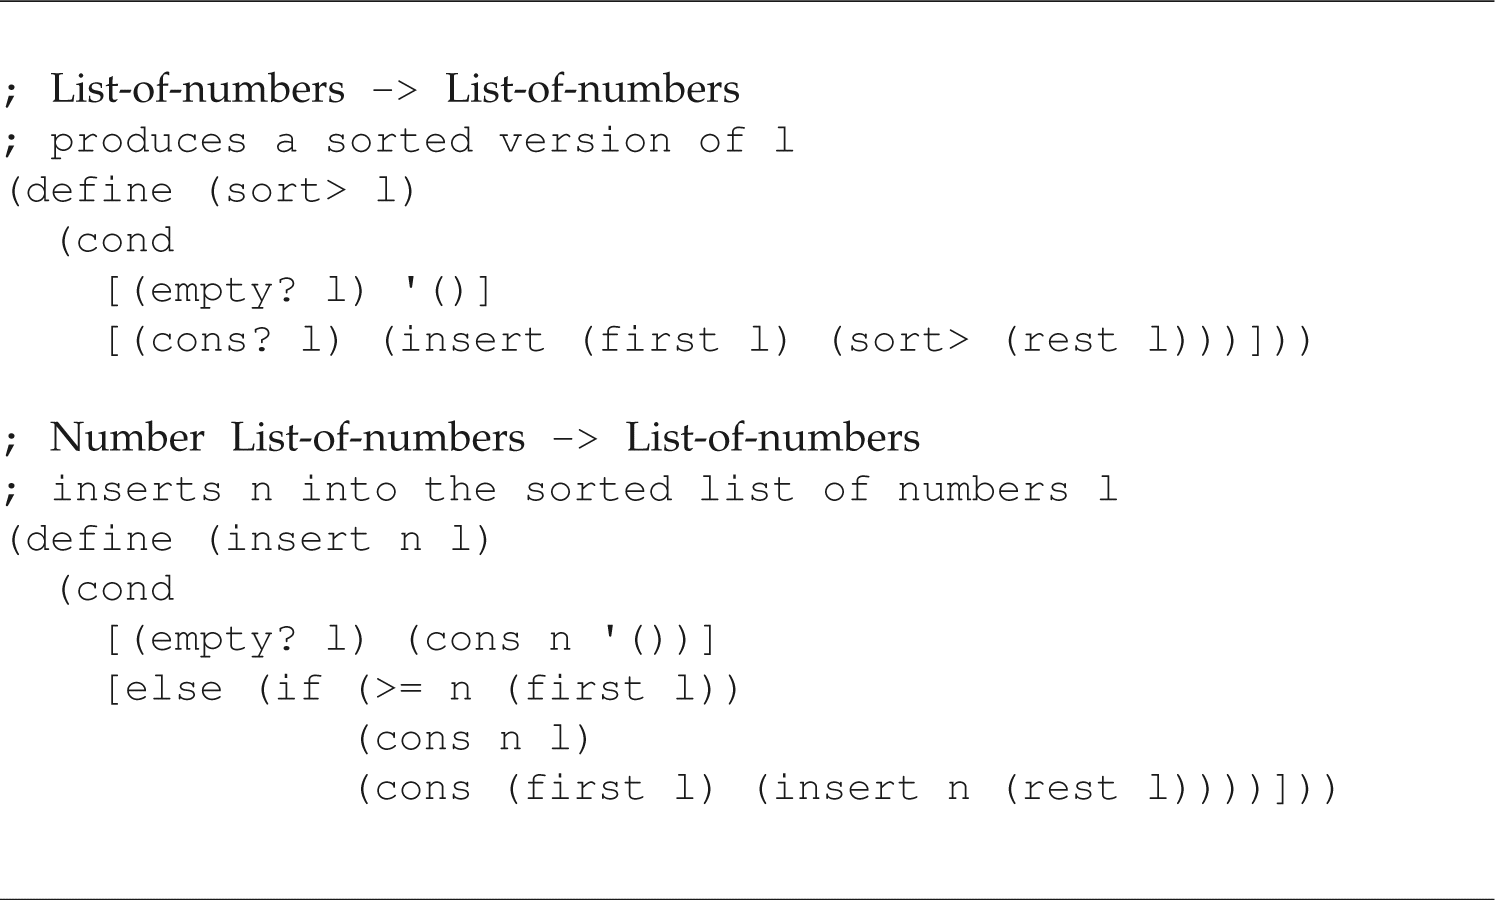
\includegraphics[width=0.85\textwidth]{images/00259.png}
  \caption{基于插入排序实现的完整排序程序}
  \label{fig:sorting_lists_of_numbers}
\end{figure}

\begin{exercise}{使用 check-satisfied 验证排序}{186}
利用练习 145 中的谓词 \code{sorted>?}，配合 \code{check-satisfied} 重新表述 \code{sort>} 的测试用例。思考如何编写测试用例来证明一个永远返回 \code{(list 9 8 7 6 5 4 3 2 1 0)} 的虚假排序函数 \code{sort>/bad} 并非真正的排序程序？
\end{exercise}

\begin{exercise}{玩家按得分排序}{187}
设计程序对游戏玩家结构体列表按分数降序排序：
\begin{lstlisting}[language=BSL]
(define-struct gp [name score])
; A GamePlayer 是结构体：(make-gp String Number)
\end{lstlisting}
\end{exercise}

\begin{exercise}{邮件排序}{188}
定义邮件结构体 \code{(make-email from date message)}。分别设计两个排序程序：一个按收信时间戳（数字）降序排序；另一个按发件人姓名（字符串）按字母表顺序排序（使用 \code{string<?}）。
\end{exercise}

\begin{exercise}{有序列表的高效搜索 search-sorted}{189}
针对已按升序排列的数字列表设计 \code{search-sorted} 函数：判断数字 $n$ 是否存在。当遇到大于 $n$ 的列表元素时，函数应当提前终止搜索。
\end{exercise}

\begin{exercise}{前缀与后缀列表生成}{190}
设计函数 \code{prefixes}：消耗字符列表并产生所有前缀构成的列表。

接着设计函数 \code{suffixes}：产生所有后缀构成的列表。
\end{exercise}

\section{通用辅助函数}
\label{sec:ch11_auxiliary_generalize}

有时一个辅助函数不仅是一个简单的帮手，更是一个\textbf{更具一般性的通用问题的解}。当我们试图直接解决某个过于狭隘的问题时，常规的设计手段可能会走入死胡同；此时退后一步，提炼出更通用的一般化任务，反而能化繁为简。

\begin{notebox}[例题：在画布中绘制多边形]
设计一个函数在给定画布上绘制任意多边形（Polygon）。
\end{notebox}

在平面几何中，多边形是由至少三个顶点（Posn）按序连线围成的闭合区域。其数据定义如下：
\begin{lstlisting}[language=BSL]
; A Polygon 是以下之一：
; -- (list Posn Posn Posn)
; -- (cons Posn Polygon)
; 解释：至少包含 3 个顶点的有序点集
\end{lstlisting}

如果我们直接尝试编写函数 \code{render-poly}：在处理基准三角形时连成闭合回路；但在递归处理多于三个点的多边形时，若直接让递归调用绘制剩余多边形，就会发现\textbf{剩余多边形的末端三点被错误地提前闭合了}（变成了图~\ref{fig:drawing_polygon} 之前描述的异常打结图形）！

\begin{figure}[htbp]
  \centering
  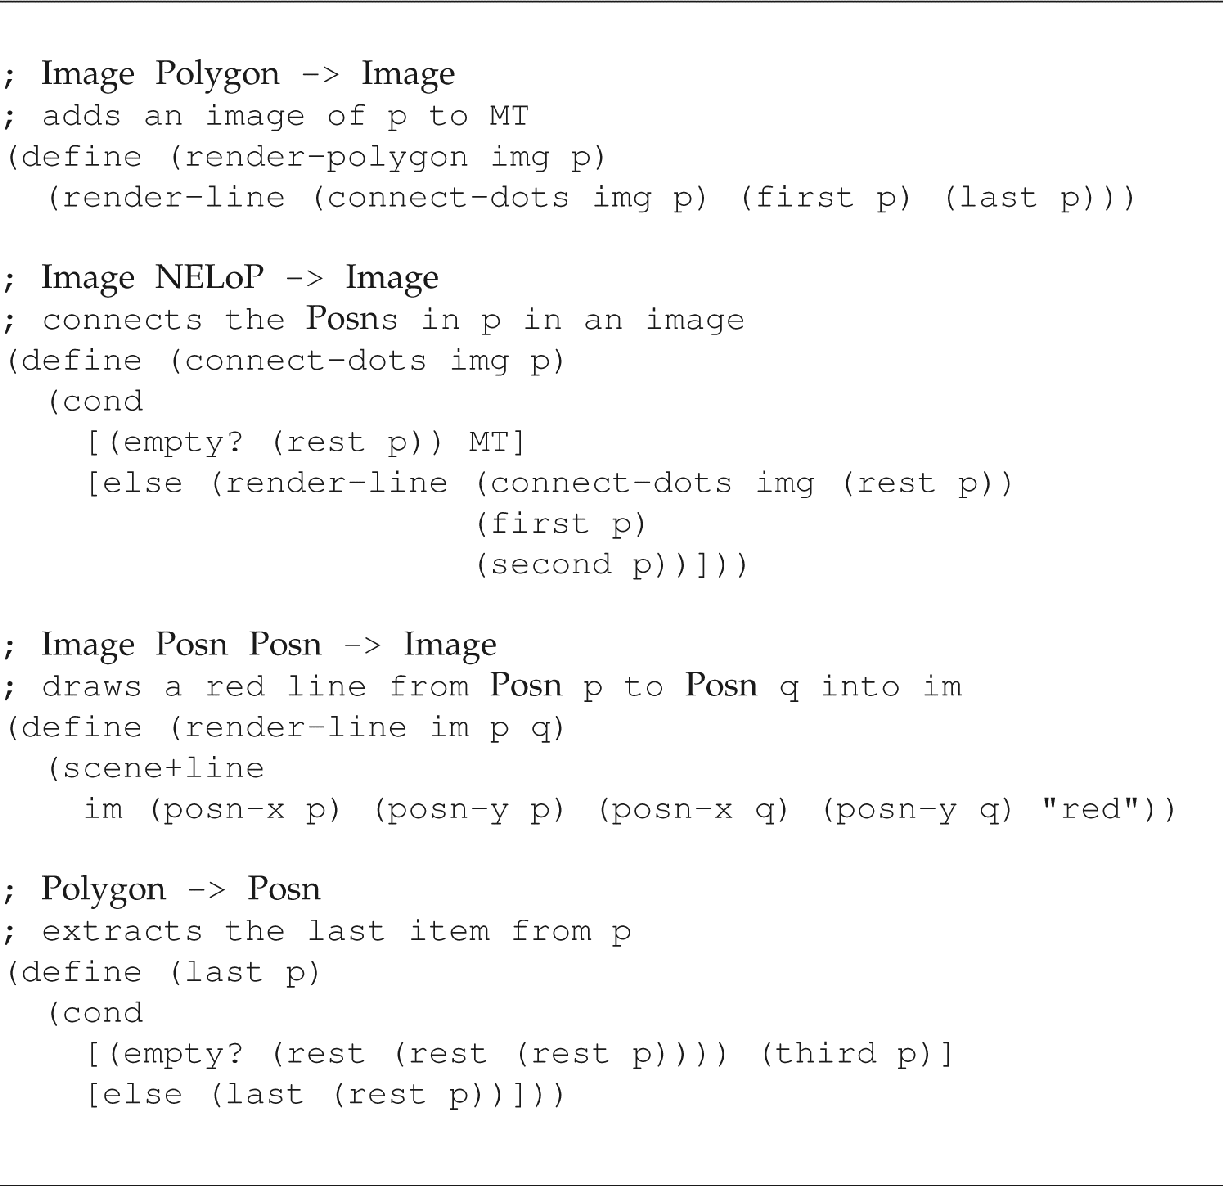
\includegraphics[width=0.85\textwidth]{images/00275.png}
  \caption{多边形绘制程序的正确设计与分解}
  \label{fig:drawing_polygon}
\end{figure}

分析该失败的根源揭示出关键洞见：绘制多边形本质上由两步组成：
\begin{enumerate}
  \item \textbf{更一般的子问题}：将任意非空点集依次连线成“开折线”（connect the dots）；
  \item \textbf{原问题的特化}：最后画一条从首顶点到末顶点的封闭边！
\end{enumerate}

为此，我们针对更通用的非空点集 \code{NELoP}（Non-Empty List of Posns）设计连线函数 \code{connect-dots}：
\begin{lstlisting}[language=BSL]
; Image NELoP -> Image
; 将 p 中的所有连续点依次用线段相连
(define (connect-dots img p)
  (cond
    [(empty? (rest p)) img]
    [else
     (render-line (connect-dots img (rest p))
                  (first p)
                  (second p))]))
\end{lstlisting}

同时为提取末顶点的需求设计辅助函数 \code{last}：
\begin{lstlisting}[language=BSL]
; NELoP -> Posn
; 提取列表中的最后一个点
(define (last p)
  (cond
    [(empty? (rest p)) (first p)]
    [else (last (rest p))]))
\end{lstlisting}

有了这两个高内聚、通用性强的辅助函数，原本复杂棘手的 \code{render-poly} 主函数竟然变成了一行优雅的组合：
\begin{lstlisting}[language=BSL]
; Image Polygon -> Image
; 在场景中绘制闭合多边形 p
(define (render-poly img p)
  (render-line (connect-dots img p)
               (first p)
               (last p)))
\end{lstlisting}

\begin{exercise}{connect-dots 示例与测试}{191}
为 \code{connect-dots} 补充完整的测试用例，涵盖单点、两点、四点的各种几何图形。
\end{exercise}

\begin{exercise}{last 函数推导与验证}{192}
解释为什么可以直接对 \code{Polygon} 调用针对 \code{NELoP} 设计的 \code{last} 函数。
\end{exercise}

\begin{exercise}{render-poly 的替代设计思路}{193}
尝试通过以下两种不同思路重构 \code{render-poly}，并确保通过测试：
\begin{enumerate}
  \item 先将末顶点 \code{(last p)} \code{cons} 到 \code{p} 的前端，然后直接调用 \code{connect-dots}；
  \item 先将首顶点 \code{(first p)} 添加到 \code{p} 的尾部，然后直接调用 \code{connect-dots}。
\end{enumerate}
\end{exercise}

\begin{exercise}{带闭合终点的 connect-dots}{194}
修改 \code{connect-dots}，令其额外接收一个指定的闭合目标点 \code{target}，使得最后一个点自动与该目标点相连。随后据此简化 \code{render-poly}。
\end{exercise}

% ==============================================================================
% 第 12 章：综合项目：列表 (Chapter 12: Projects: Lists)
% ==============================================================================

\chapter{综合项目：列表}
\label{sec:ch12_projects}

本章提供了一组综合性项目练习，旨在全面巩固你对程序设计核心要素的理解：批处理与交互式程序设计、基于组合的设计思想、愿望清单管理、以及针对自引用数据的设计配方。

本章首先探讨现实世界的大规模数据处理：英语词典与 iTunes 音乐库；接着通过两个小节剖析单词字谜游戏，展示如何将复杂问题解构为高内聚子任务；随后的章节带领你通过\term{迭代细化}（iterative refinement）开发贪吃蛇、俄罗斯方块、太空大战等经典游戏；最后一节则实现能够解释执行正则表达式与通用有限状态机的模拟引擎。

\section{现实世界的数据：词典}
\label{sec:ch12_dictionaries}

现实世界中的信息往往以极其庞大的规模出现，这正是编写程序处理它们的意义所在。例如，一本英语词典并非包含十几个单词，而是收录数十万个词条。在处理如此大规模的数据时，必须严格遵循设计配方：先在小型输入样例上精心设计并验证函数逻辑，一旦确信无误，再将其投入到真实的真实世界数据中运行。如果程序运行过于缓慢，请反思函数内部是否存在冗余的重复遍历或计算。

\begin{figure}[htbp]
  \centering
  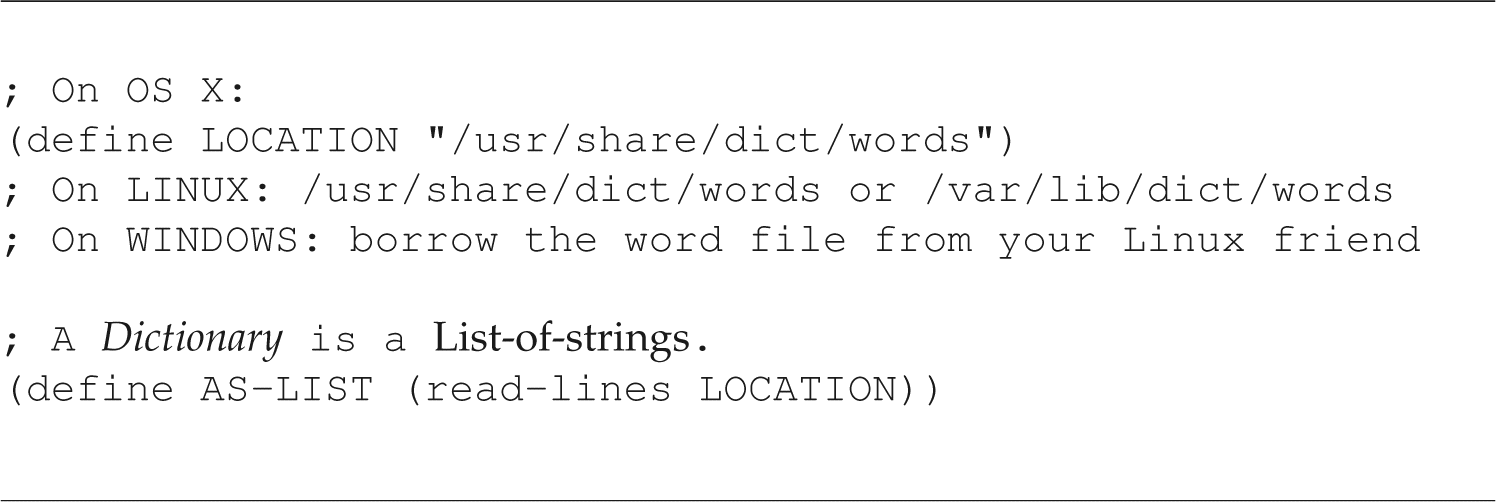
\includegraphics[width=0.85\textwidth]{images/00276.png}
  \caption{从操作系统中读取整本英语词典}
  \label{fig:reading_dictionary}
\end{figure}

在 BSL+ 中，通过 \code{2htdp/batch-io} 库中的 \code{read-words} 函数，只需一行代码即可将系统的整本英语词典加载为一个庞大的字符串列表（如图~\ref{fig:reading_dictionary} 所示）。

在下列练习中，字母扮演着重要角色，我们定义所有英文字母的列表：
\begin{lstlisting}[language=BSL]
; A Letter 是以下单字符 1String 之一：
; -- "a"
; -- ...
; -- "z"
(define LETTERS (explode "abcdefghijklmnopqrstuvwxyz"))
\end{lstlisting}

\begin{exercise}{统计指定字母开头的单词数 starts-with\#}{195}
设计函数 \code{starts-with\#}：接收一个 \code{Letter} 与一个 \code{Dictionary}（单词列表），统计词典中有多少个单词以该指定字母开头。验证函数正确后，统计你的计算机词典中以 \code{"e"} 和以 \code{"z"} 开头的单词数量。
\end{exercise}

\begin{exercise}{全字母词频统计 count-by-letter}{196}
设计结构体与数据定义 \code{Letter-Count}，用于保存一个字母及其对应的词频统计数：
\begin{lstlisting}[language=BSL]
(define-struct lc [letter count])
; A Letter-Count 是一个结构体：(make-lc Letter Number)
\end{lstlisting}
接着设计函数 \code{count-by-letter}：接收一个 \code{Dictionary}，统计 26 个英文字母各自作为单词首字母的出现频率，返回一个 \code{Letter-Count} 列表。
\end{exercise}

\begin{exercise}{寻找最常见首字母 most-frequent}{197}
设计函数 \code{most-frequent}：接收一个 \code{Dictionary}，返回作为首字母出现次数最多的那个 \code{Letter-Count}。你的词典中最频繁出现的首字母是哪一个？它出现了多少次？
\end{exercise}

\begin{exercise}{按首字母分组与中间结构消除（Deforestation 优化）}{198}
设计函数 \code{words-by-first-letter}：接收一个 \code{Dictionary}，产生一个由词典构成的列表（\code{List-of-Dictionary}），每个子词典汇集以某一特定字母开头的单词。

随后利用该函数重构练习 197 中的 \code{most-frequent} 为 \code{most-frequent.v2}，并验证两个版本在真实词典上的输出完全一致。

\begin{notebox}[编程语境：中间数据结构与“森林砍伐” (Deforestation)]
第二种设计方案通过构建庞大的中间分组词典列表来计算最终结果，这些中间数据除了供后续统计之外并无其他作用。在现代高级语言编译器中，有时会自动执行“森林砍伐”（Deforestation，即消除中间数据结构）优化，将两个连续遍历的函数融合为一个，从而消除中间数据结构带来的内存与遍历开销。在未启用此类优化的语言中，如果程序运行缓慢，应考虑避免创建不必要的中间数据结构。
\end{notebox}
\end{exercise}

\section{现实世界的数据：iTunes 播放列表}
\label{sec:ch12_itunes}

苹果公司的 iTunes（以及随后的 Music 应用）能够将其媒体数据库导出为标准的 XML 文件。借助 \code{2htdp/itunes} 教学库，我们能够将音乐曲目导入 BSL 程序进行查询与统计。

在本节中，我们考察两种不同的数据表示法：
\begin{enumerate}
  \item \textbf{基于结构体的表示}（\code{Track} 和 \code{Date}，如图~\ref{fig:itunes_structures} 与图~\ref{fig:itunes_functions} 所示）：每个曲目具有固定的 8 个字段，属性完备、强类型化。
  \item \textbf{基于关联列表的表示}（\code{LLists}，如图~\ref{fig:itunes_lists} 所示）：采用半结构化（semi-structured）键值对列表，允许各曲目包含不同数量的非规范化属性。
\end{enumerate}

\begin{figure}[htbp]
  \centering
  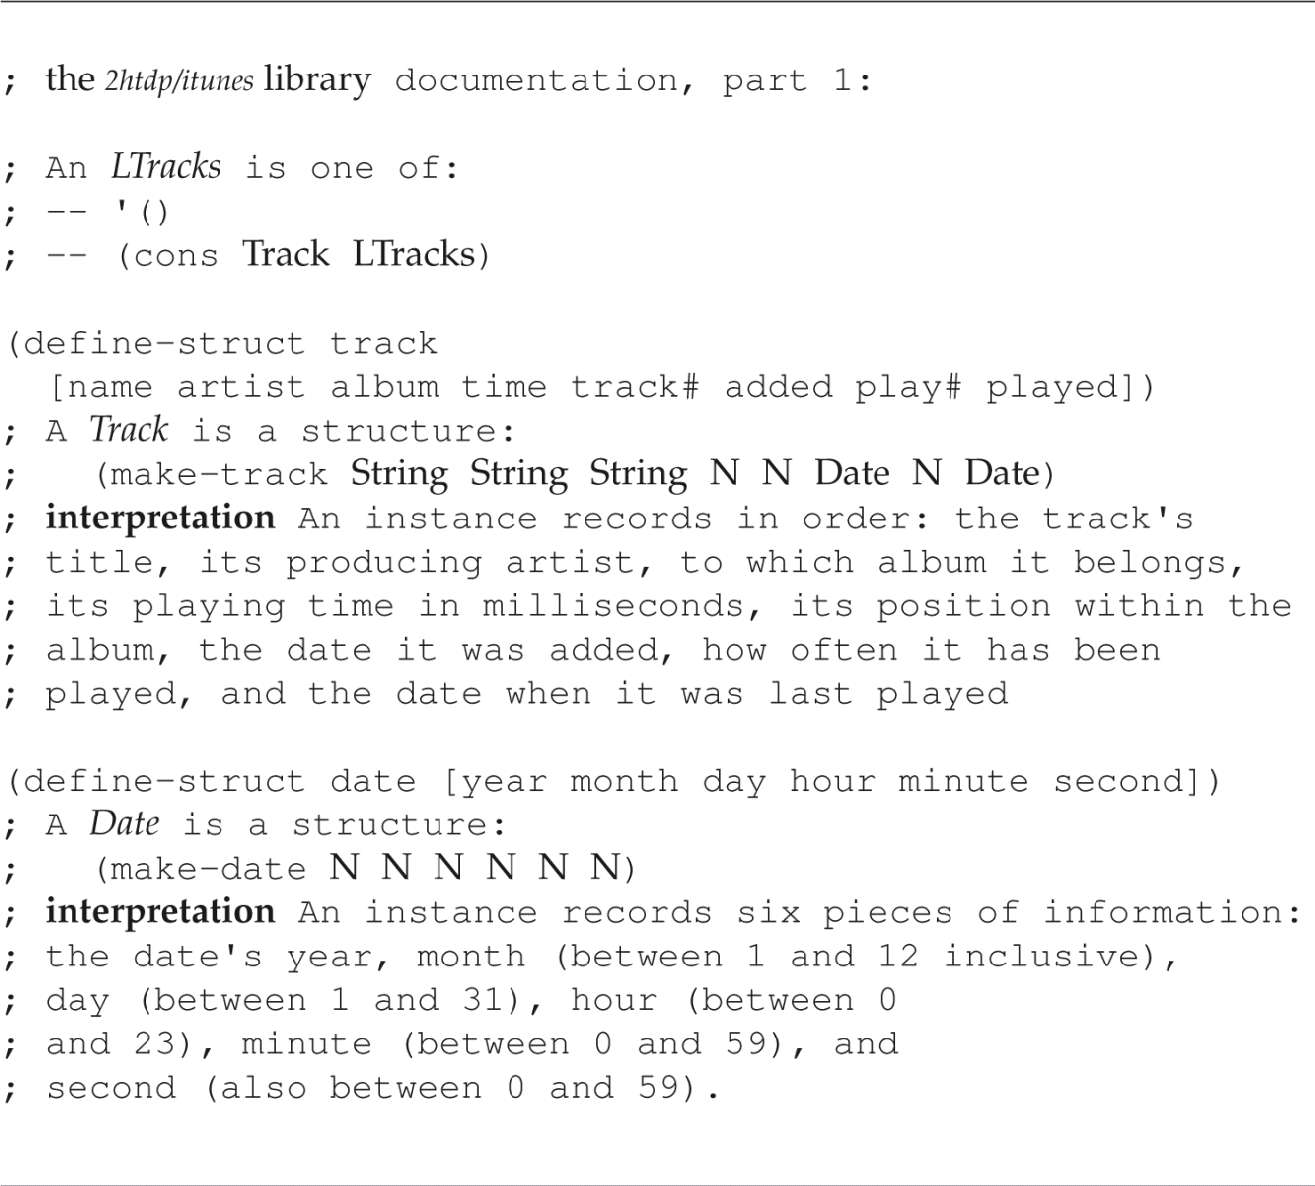
\includegraphics[width=0.85\textwidth]{images/00277.png}
  \caption{基于结构体的 iTunes 曲目数据定义}
  \label{fig:itunes_structures}
\end{figure}

\begin{figure}[htbp]
  \centering
  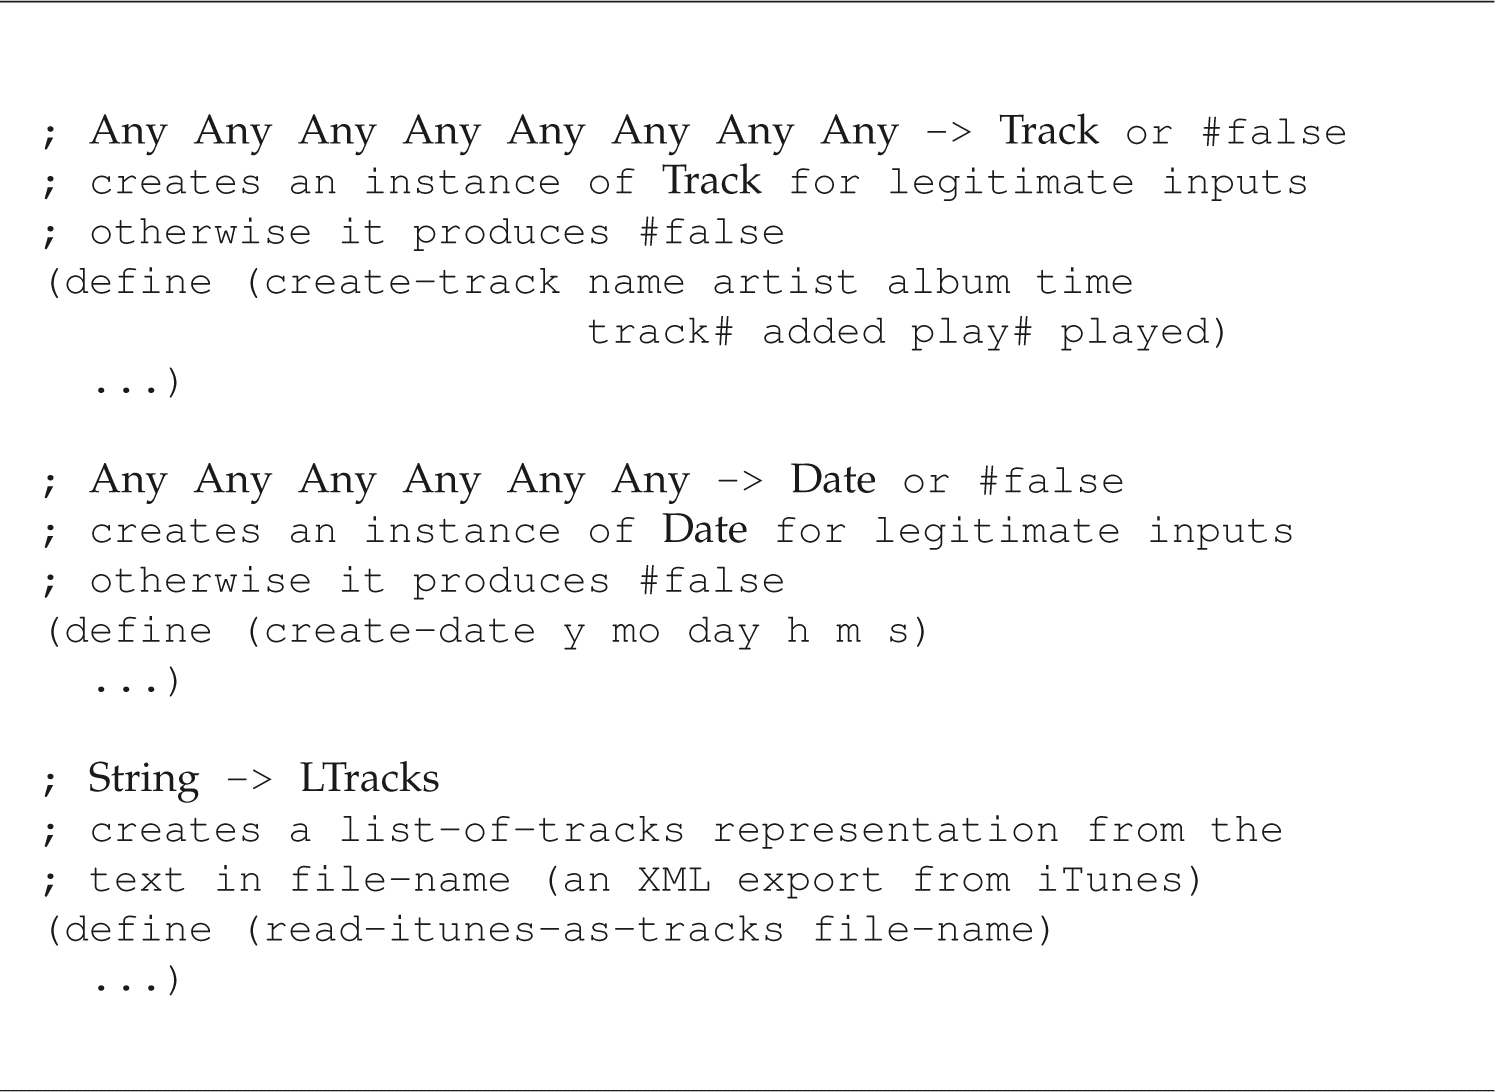
\includegraphics[width=0.85\textwidth]{images/00278.png}
  \caption{iTunes 库函数接口}
  \label{fig:itunes_functions}
\end{figure}

\begin{exercise}{构造曲目示例}{199}
构造若干 \code{Date}、\code{Track} 和 \code{LTracks}（曲目列表）的示例，用于后续测试。
\end{exercise}

\begin{exercise}{累计播放时长 total-time}{200}
设计函数 \code{total-time}：接收一个 \code{LTracks}，计算并返回所有曲目的总播放时间（单位：毫秒）。
\end{exercise}

\begin{exercise}{提取不重复专辑名 select-album-titles/unique}{201}
设计函数 \code{select-all-album-titles}：提取 \code{LTracks} 中的所有专辑名称（可能包含重复项）。

接着设计集合去重函数 \code{create-set}：消耗字符串列表，返回去除了所有重复项的集合列表。

最后组合二者实现 \code{select-album-titles/unique}，输出所有独一无二的专辑名称列表。
\end{exercise}

\begin{exercise}{专辑查询 select-album}{202}
设计函数 \code{select-album}：消耗专辑名称与 \code{LTracks}，提取并返回属于该专辑的所有曲目列表。
\end{exercise}

\begin{exercise}{按日期筛选 select-album-date}{203}
设计函数 \code{select-album-date}：消耗专辑名、指定日期 \code{Date} 以及 \code{LTracks}，筛选出属于该专辑且在指定日期之后播放过的所有曲目。
\end{exercise}

\begin{exercise}{数据库查询：按专辑分组 select-albums}{204}
设计函数 \code{select-albums}：消耗 \code{LTracks}，返回一个由曲目列表构成的列表（\code{List-of-LTracks}），其中每个子列表包含且仅包含属于同一张专辑的所有曲目。
\end{exercise}

\begin{figure}[htbp]
  \centering
  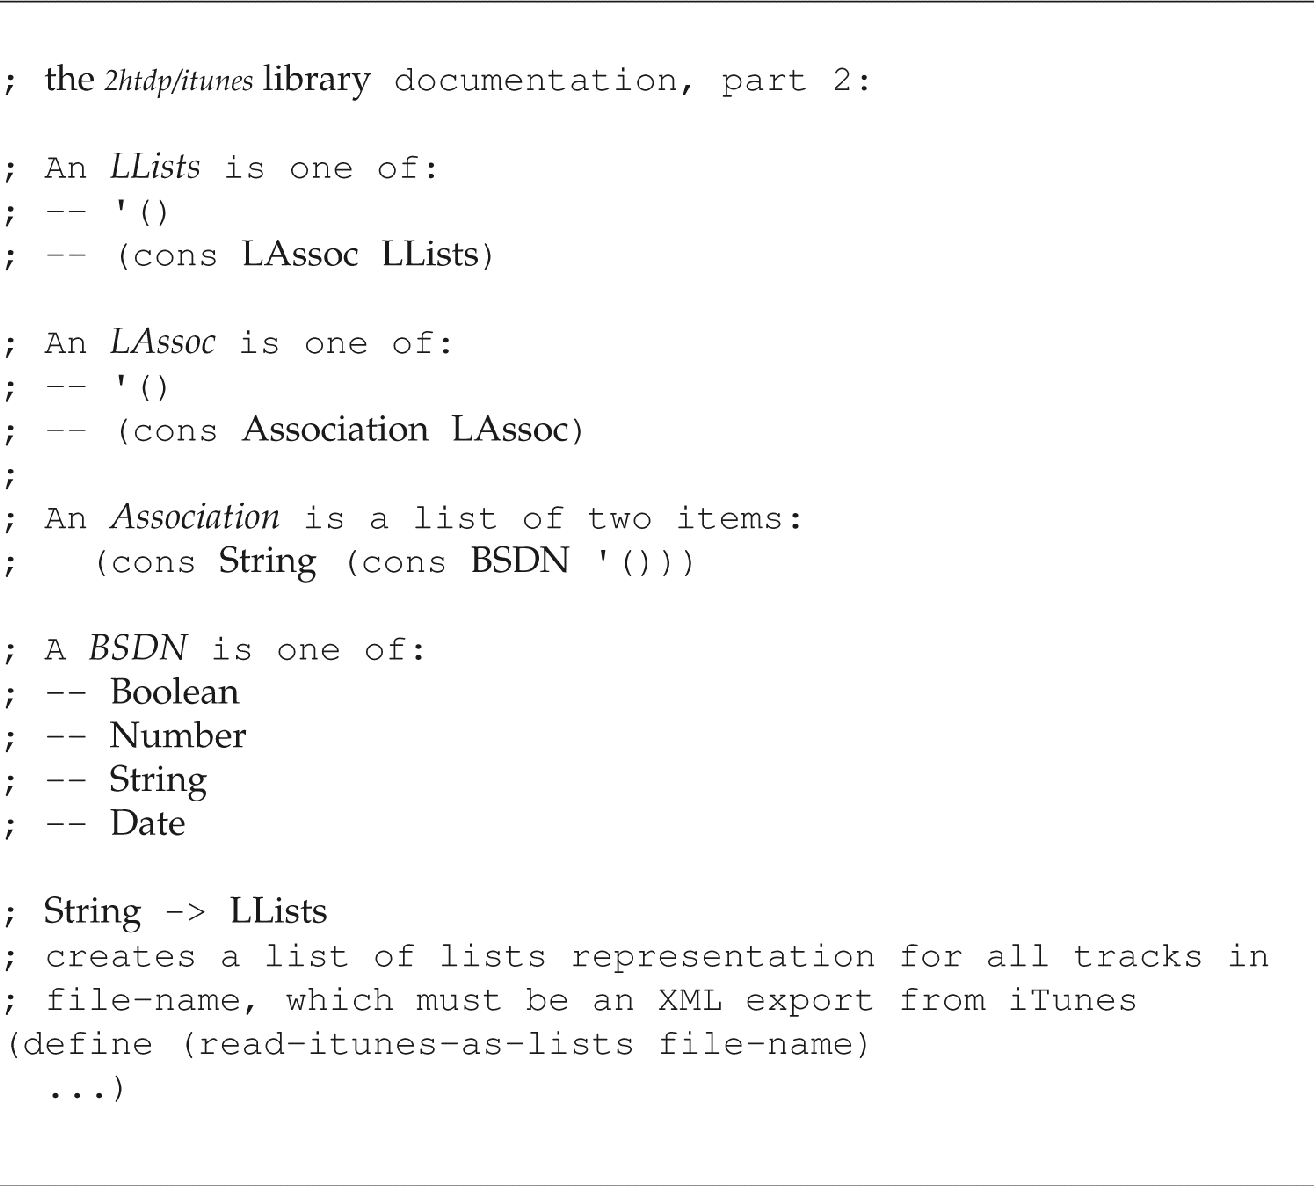
\includegraphics[width=0.85\textwidth]{images/00279.png}
  \caption{基于键值对关联列表的 iTunes 数据表示}
  \label{fig:itunes_lists}
\end{figure}

\begin{exercise}{半结构化曲目示例与查询 find-association}{205}
构造图~\ref{fig:itunes_lists} 中 \code{LAssoc} 与 \code{LLists} 的具体示例。
\end{exercise}

\begin{exercise}{关联查找函数 find-association}{206}
设计函数 \code{find-association}：消耗键名 \code{key}（字符串）、关联列表 \code{LAssoc} 以及默认值 \code{default}。返回首个键名为 \code{key} 的关联项；若未找到，则返回 \code{default}。
\end{exercise}

\begin{exercise}{基于列表表示的播放时长统计}{207}
针对 \code{LLists} 设计 \code{total-time/list} 函数，计算总播放时长。
\end{exercise}

\begin{exercise}{布尔属性提取 boolean-attributes}{208}
设计函数 \code{boolean-attributes}：提取并返回其属性值为布尔类型的所有属性名称列表（去重后）。
\end{exercise}

\section{单词游戏：图解组合设计}
\label{sec:ch12_word_games_composition}

许多人都喜欢字谜游戏。考虑以下例题：
\begin{notebox}[字谜求解]
给定一个英文单词，找出所有由完全相同字母构成的合法英文单词（换位词，Anagram）。例如输入 \code{"cat"}，其字母排列组合还可构成合法词 \code{"act"}。
\end{notebox}

例如对于单词 \code{"dear"}，其 4 个字母共有 $4! = 24$ 种排列方式，其中在词典中合法存在的单词有 3 个：\code{"read"}、\code{"dear"} 和 \code{"dare"}。

人工解决此问题的思路是：先枚举出给定单词中所有字母的所有可能排列组合，然后再逐一查词典，保留那些真正属于词典的单词。这天然指导我们将程序分解为若干函数的串联组合：
\begin{lstlisting}[language=BSL]
; String -> List-of-strings
; 查找由 s 的所有字母构成的所有同字母异序词
(define (alternative-words s)
  (in-dictionary
    (words->strings
      (arrangements (string->word s)))))
\end{lstlisting}

图~\ref{fig:finding_alternative_words} 展示了这一高层组合设计的架构与各函数的职责划分。

\begin{figure}[htbp]
  \centering
  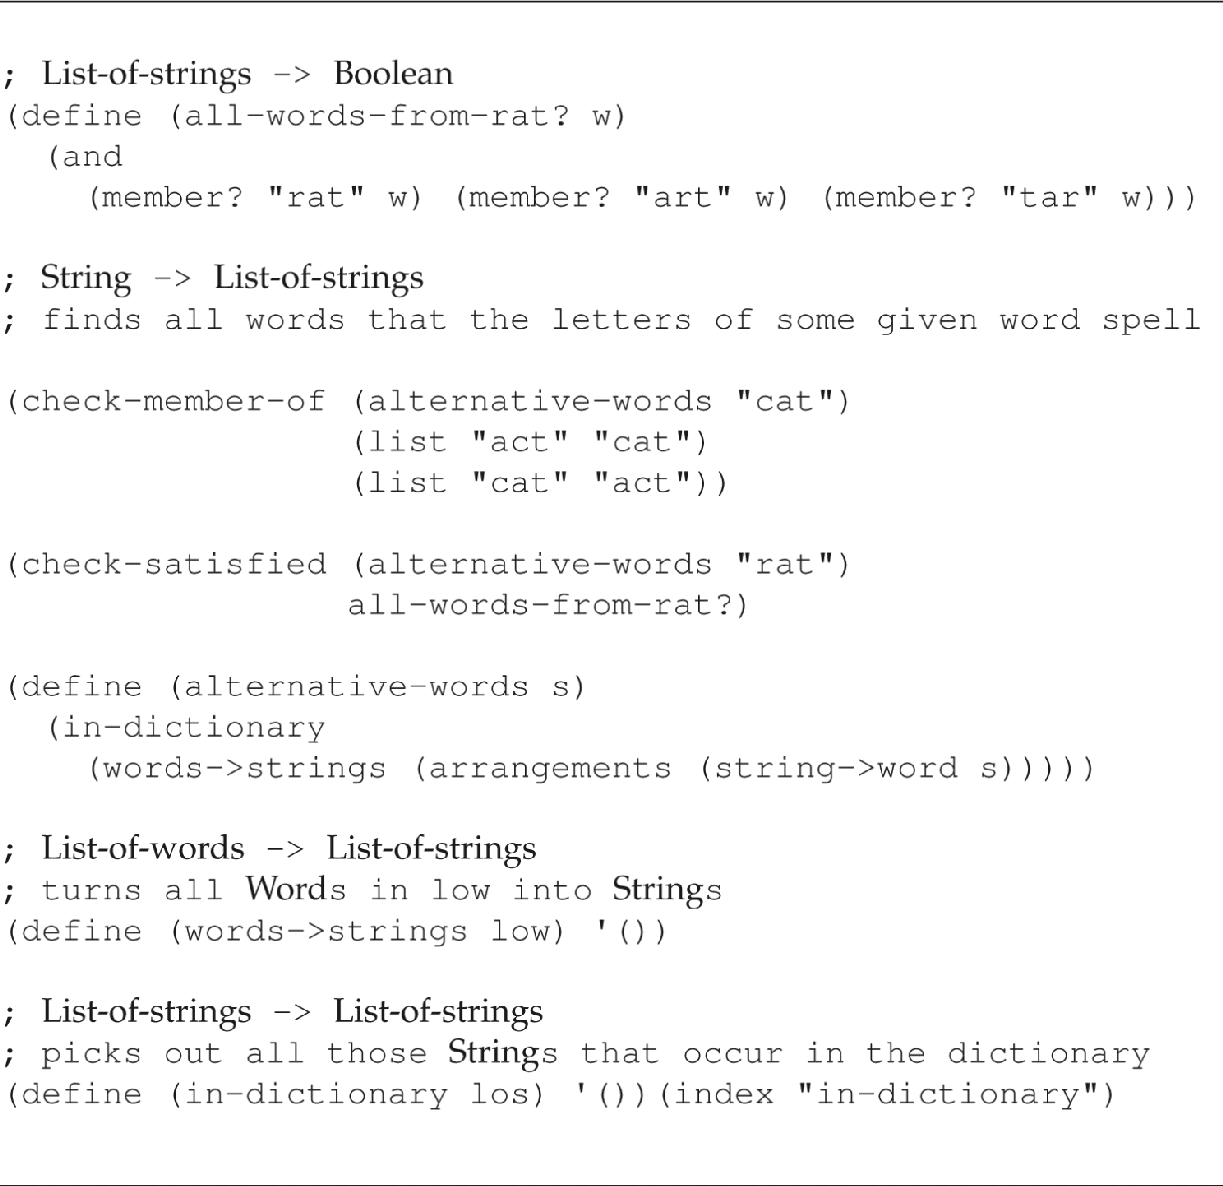
\includegraphics[width=0.85\textwidth]{images/00284.png}
  \caption{单词异序词查找程序的组合设计架构}
  \label{fig:finding_alternative_words}
\end{figure}

\begin{exercise}{字符串与单词表示的双向转换}{209}
为了便于递归重排字符，我们使用单字符列表 \code{Word} 表示单词：
\begin{lstlisting}[language=BSL]
; A Word 是以下之一：
; -- '()
; -- (cons 1String Word)
\end{lstlisting}
利用内置的 \code{explode} 与 \code{implode} 设计 \code{string->word} 与 \code{word->string}。
\end{exercise}

\begin{exercise}{单词列表批量转换为字符串列表 words->strings}{210}
设计函数 \code{words->strings}：消耗 \code{List-of-words} 并产生对应的 \code{List-of-strings}。
\end{exercise}

\begin{exercise}{词典有效性过滤 in-dictionary}{211}
设计函数 \code{in-dictionary}：消耗字符串列表，筛选并仅保留那些收录在系统词典中的合法单词。
\end{exercise}

\section{单词游戏：问题的核心}
\label{sec:ch12_word_games_heart}

本节解决整个字谜程序的核心与难点：设计函数 \code{arrangements}，计算一个 \code{Word} 的全排列（Permutations）。

\begin{exercise}{全排列数据定义与示例}{212}
写出 \code{List-of-words} 的自引用数据定义，并针对两字母单词（如 \code{"d"} 和 \code{"e"}）编写全排列的功能示例。
\end{exercise}

对于一个单词 \code{w}：
\begin{itemize}
  \item 若为空词 \code{'()}，其全排列仅有唯一一种可能：\code{(list '())}；
  \item 若为非空词，自然递归 \code{(arrangements (rest w))} 将求出剩余所有字符的全排列；
  \item 此时，主任务转化为：\textbf{如何将首字符 \code{(first w)} 插入到上述每个单词的所有可能缝隙中（开头、中间所有位置、末尾）}！
\end{itemize}

我们将这一新任务委托给辅助函数 \code{insert-everywhere/in-all-words}：
\begin{lstlisting}[language=BSL]
(define (arrangements w)
  (cond
    [(empty? w) (list '())]
    [else (insert-everywhere/in-all-words (first w)
                                          (arrangements (rest w)))]))
\end{lstlisting}

\begin{exercise}{全缝隙插入函数 insert-everywhere/in-all-words}{213}
设计函数 \code{insert-everywhere/in-all-words}：消耗单字符 1String 与单词列表，将该字符插入到每个单词的每一个可能位置（使用 \code{append} 拼接列表）。
\end{exercise}

\begin{exercise}{联调集成与端到端运行}{214}
将 \code{arrangements} 与 12.3 节的模块整合，运行全套测试，并在真实词汇上进行字谜求解实验。
\end{exercise}

\section{喂贪吃蛇}
\label{sec:ch12_feeding_worms}

贪吃蛇（Worm / Snake）是经典的街机游戏：蛇在屏幕中移动，玩家通过方向键改变其前进方向；每吃到一个食物，蛇身增长一节并获得分数；若蛇头触碰边界或咬到自身躯干，游戏即告结束（如图~\ref{fig:playing_worm} 所示）。

\begin{figure}[htbp]
  \centering
  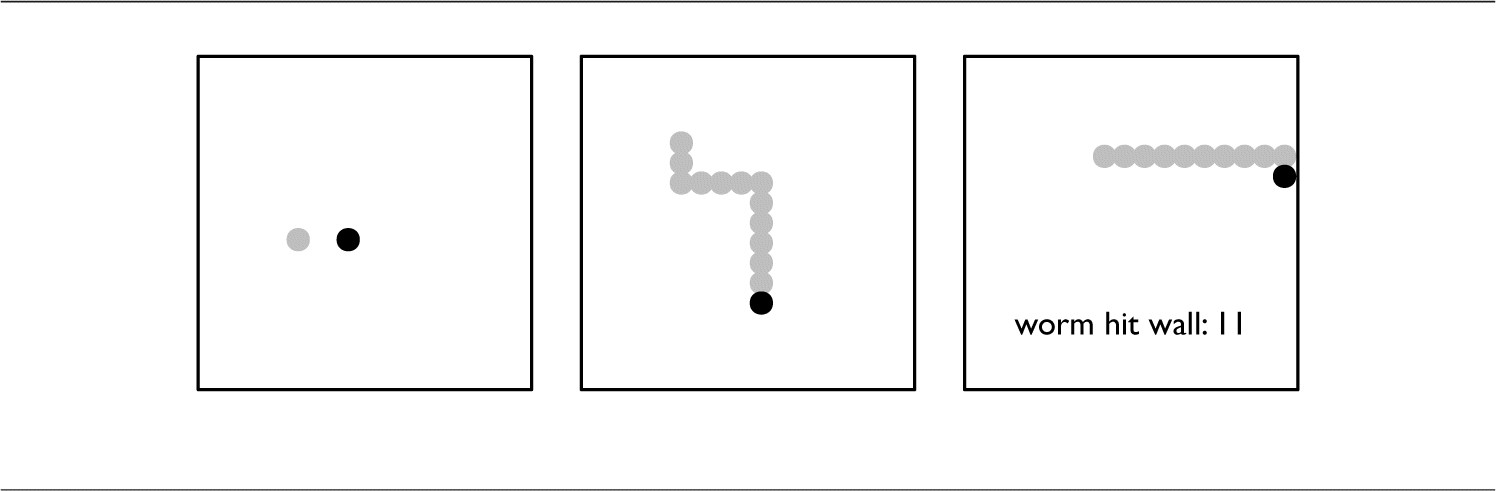
\includegraphics[width=0.85\textwidth]{images/00289.png}
  \caption{贪吃蛇游戏截图}
  \label{fig:playing_worm}
\end{figure}

我们将通过迭代细化逐步构建整个游戏：

\begin{exercise}{第一阶段：单节蛇与方向控制}{215}
设计一个世界程序：蛇由单个红色圆盘（蛇头）构成，每个时钟节拍沿当前方向前进一个圆盘直径的距离，玩家可通过四个方向键改变行进方向。
\end{exercise}

\begin{exercise}{第二阶段：触壁死亡判定}{216}
为练习 215 的程序添加触壁检测：当蛇头触及画布边界时停止游戏，并在画面左下角渲染提示文本 \code{"worm hit border"}。
\end{exercise}

\begin{exercise}{第三阶段：多节蛇身游动}{217}
将蛇身的数据表示泛化为 \code{Posn} 列表（表头为蛇头，其余为按序跟随的躯干节点）。实现多节蛇身的平滑游动（提示：每次前进时在蛇头方向 \code{cons} 一个新节点，并切除尾部的最后一个节点）。
\end{exercise}

\begin{exercise}{第四阶段：自身碰撞检测}{218}
完善游戏结束规则：当蛇头与自身现存的任意躯干节点坐标重合时，判定游戏结束并显示撞击自身提示。
\end{exercise}

\begin{exercise}{第五阶段：投放食物与得分增长}{219}
引入随机放置的食物（如图~\ref{fig:random_food} 所示的生成逻辑）。当蛇头覆盖食物坐标时，吃掉食物并将身体延长一节，同时在随机位置刷新下一枚食物。
\end{exercise}

\begin{figure}[htbp]
  \centering
  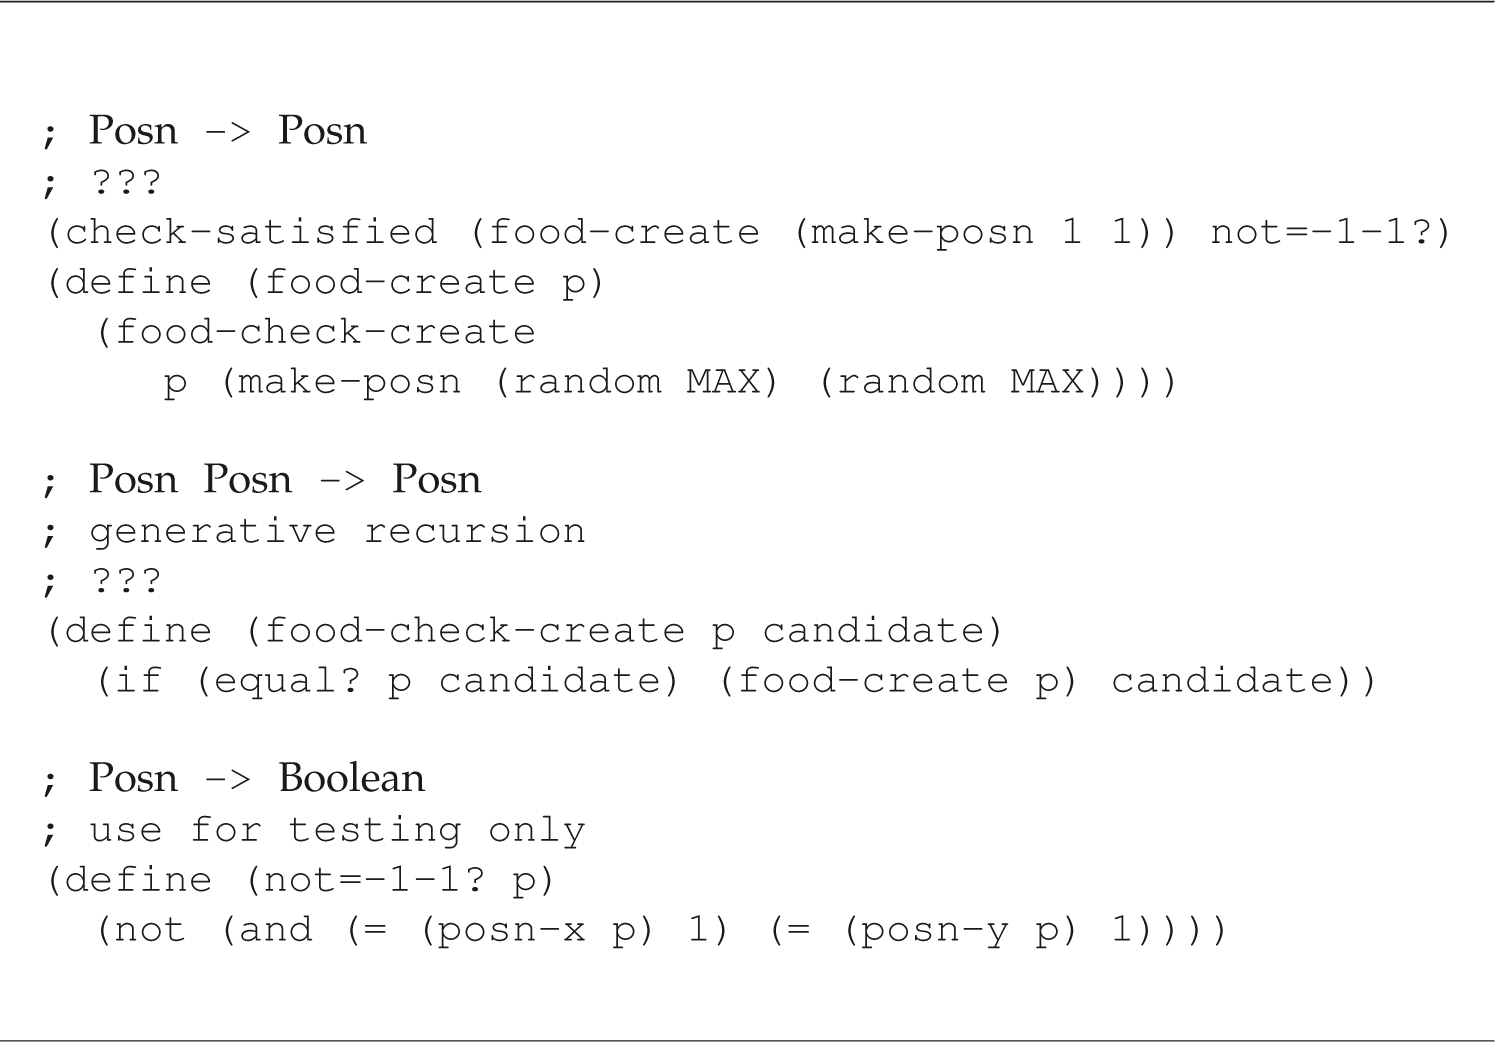
\includegraphics[width=0.85\textwidth]{images/00290.png}
  \caption{食物的随机坐标生成逻辑}
  \label{fig:random_food}
\end{figure}

\section{简易俄罗斯方块}
\label{sec:ch12_simple_tetris}

俄罗斯方块（Tetris）是另一款风靡全球的经典游戏。在此项目中，我们实现一个规则精炼的简易版本：单个方块从顶部缓慢坠落，玩家可通过左右方向键调整其下落列位置；一旦方块触底或叠落在已有方块之上，它便冻结在原地，随后顶部重新生成新的方块；当堆叠高度触及画布顶端时，游戏结束（如图~\ref{fig:simple_tetris} 所示）。

\begin{figure}[htbp]
  \centering
  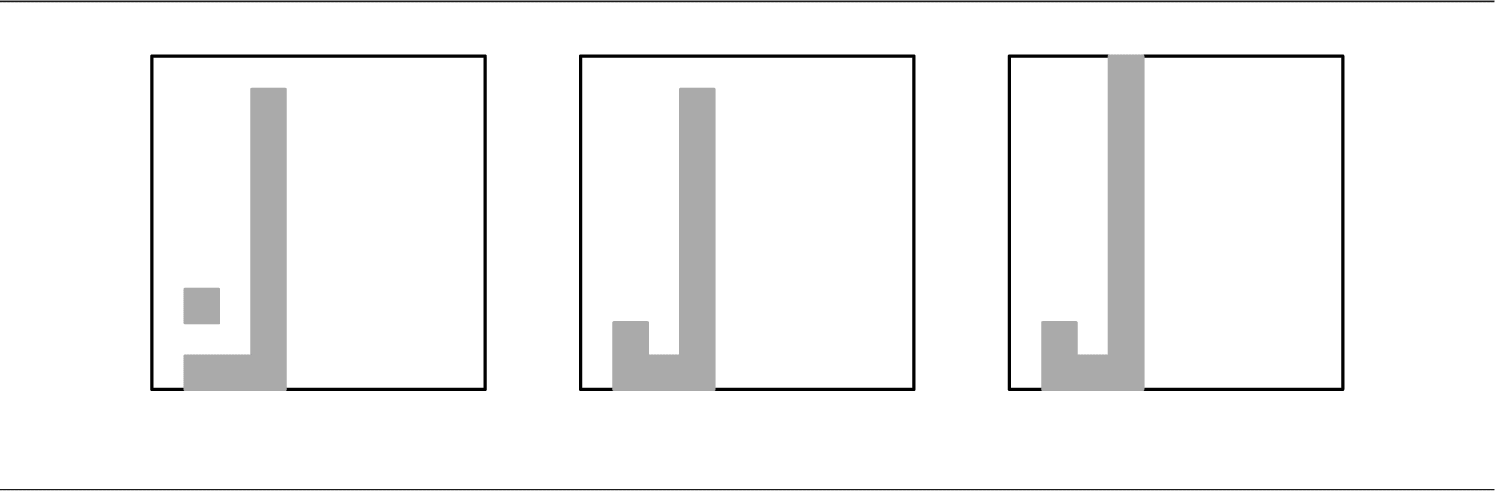
\includegraphics[width=0.75\textwidth]{images/00291.png}
  \caption{简易俄罗斯方块游戏示意图}
  \label{fig:simple_tetris}
\end{figure}

世界状态数据定义采用网格逻辑坐标：
\begin{lstlisting}[language=BSL]
(define-struct tetris [block landscape])
(define-struct block [x y])

; A Tetris 是一个结构体：(make-tetris Block Landscape)
; A Landscape（地貌列表）是以下之一：
; -- '()
; -- (cons Block Landscape)
; A Block 是一个结构体：(make-block N N)
; 解释：block 代表当前正在下落的方块；landscape 代表已经着陆堆叠的所有方块。
\end{lstlisting}

\begin{exercise}{渲染游戏场景 tetris-render}{220}
设计函数 \code{tetris-render}：将当前的 \code{Tetris} 状态（包含下落方块与静态地貌方块列表）绘制在网格画布上。
\end{exercise}

\begin{exercise}{下落与堆叠判定 tetris-main}{221}
编写时钟更新函数：方块垂直下落；当检测到方块触底或下移一步将与地貌中的某个方块重叠时，将当前方块冻结并转移入地貌列表，并生成一个新方块。
\end{exercise}

\begin{exercise}{水平移动控制}{222}
添加键盘事件处理：响应左右方向键移动下落方块，并防止方块穿透侧壁或嵌入侧边已有的方块堆中。
\end{exercise}

\begin{exercise}{顶格游戏结束判定}{223}
使用 \code{stop-when} 监听：当任何一列的方块堆叠触及顶部边界时终止游戏，并展示最终得分。
\end{exercise}

\section{完整的太空大战}
\label{sec:ch12_full_space_war}

\begin{exercise}{综合世界项目：太空入侵者}{224}
综合运用本章所学的多对象列表控制技术，将第 6 章的飞碟入侵防御游戏完善为全功能版：坦克可在地面自由移动，并可任意发射多枚导弹；飞碟以特定轨迹降落并可投掷炸弹；实现弹幕与飞碟的精准碰撞判定。
\end{exercise}

\begin{exercise}{创意设计：森林灭火飞行模拟}{225}
设计空中灭火游戏：模拟森林发生随机野火，玩家驾驶消防飞机水平巡航并适时投放水弹灭火，在限定时间内扑灭所有林火。
\end{exercise}

\section{有限状态机}
\label{sec:ch12_finite_state_machines}

\term{有限状态机}（Finite State Machines, FSM）是计算机科学的基石理论之一。在第 4.7 节中，我们曾通过硬编码的条件分支实现过交通信号灯。现在，我们能够设计一个通用的\term{状态机解释器}：它接受任意状态机的数据描述，并驱动其运行。

图~\ref{fig:general_fsm} 给出了通用的状态机数据定义与交互模拟模型。

\begin{figure}[htbp]
  \centering
  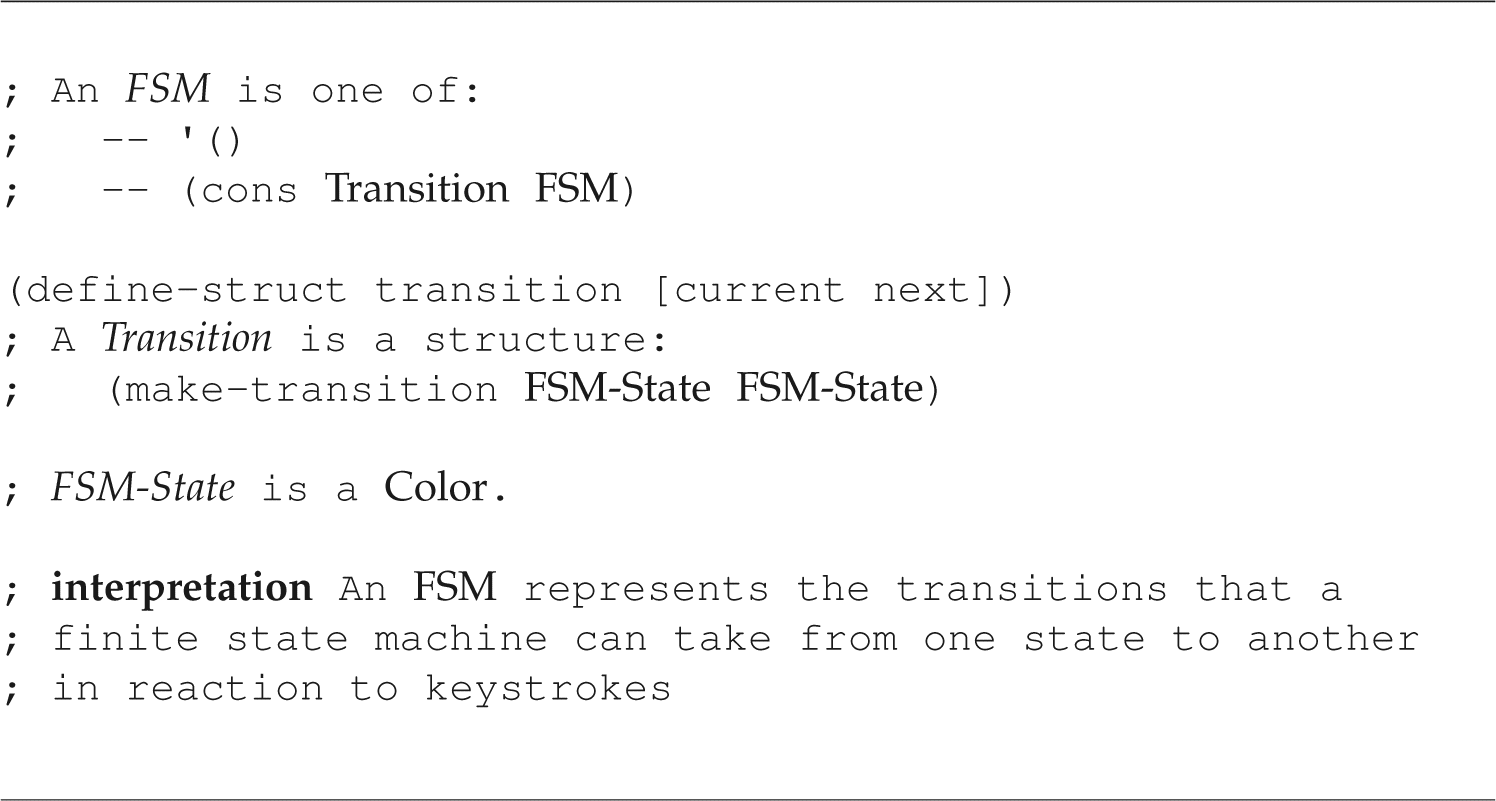
\includegraphics[width=0.85\textwidth]{images/00295.png}
  \caption{通用有限状态机的数据表示与模拟器框架}
  \label{fig:general_fsm}
\end{figure}

\begin{exercise}{状态判等谓词 state=?}{226}
设计谓词 \code{state=?}：判断两个状态是否相等。
\end{exercise}

\begin{exercise}{黑白跳变状态机 BW Machine}{227}
构造一个每按任意键就在黑白两色之间往复跳变的状态机数据实例。
\end{exercise}

\begin{exercise}{状态跳转查找函数 find}{228}
设计函数 \code{find}：在转移列表 \code{FSM} 中查找当前状态匹配的转移规则，并输出下一状态。
\end{exercise}

\begin{exercise}{按键驱动的状态转移 Transition.v2}{229}
扩展转移规则结构体为 \code{(make-ktransition current key next)}，使状态转移严格依赖玩家所按下的特定按键。
\end{exercise}

\begin{exercise}{带初始与终止状态的终极 FSM 解释器}{230}
设计完整版数据模型 \code{(make-fsm initial transitions final)}，并实现通用解释器 \code{fsm-simulate}：当状态机流转到达终止状态时，自动平稳退出。
\end{exercise}

% ==============================================================================
% 第 13 章：第二部分小结 (Chapter 13: Summary)
% ==============================================================================

\chapter{第二部分小结}
\label{sec:ch13_summary}

本书的第二部分专注于\term{处理任意大小数据}（Arbitrarily Large Data）的程序设计。正如你所体会到的，当软件能够处理没有预设大小限制的海量信息时，其价值才真正得以释放。掌握“任意大小的数据”是迈向真正职业程序员道路上的决定性一步。在此，我们建议你牢记以下三条核心经验：

\begin{notebox}[第二部分核心收获]
\begin{enumerate}
  \item \textbf{自引用与交叉引用的设计配方细化}：
  本部分对设计配方进行了重大扩展，使其能够系统化地应对数据定义中的\textbf{自引用}与\textbf{交叉引用}。
  \begin{itemize}
    \item 数据定义中出现自引用，必然指导我们在函数模板与函数体中构建对应的\term{结构型递归调用}；
    \item 数据定义中出现对其他复杂数据定义的交叉引用，必然指导我们设计专门处理对应数据的\term{独立辅助函数}。
  \end{itemize}

  \item \textbf{分解与组合的设计范式 (Design by Composition)}：
  复杂问题必然要求分解为相互协作的子任务。当你分解一个问题时，需要两个支撑要素：分别解决各子任务的函数，以及用于组合这些独立解的数据定义。
  为了确保在耗费精力完成各个独立函数后整体系统能够严丝合缝地协同工作，你必须\textbf{严格制定包含明确函数签名、目的说明与接口契约的“愿望清单”（Wish List）}。
  
  在以下三种情形中，“分解—组合”的设计手法尤为关键：
  \begin{itemize}
    \item 问题描述中明确或隐含了不同专业维度的辅助任务；
    \item 函数体的编写需要遍历另一个任意大小的数据集合；
    \item 求解一个\textbf{更一般化、更通用的问题}往往比直接求解原始特定问题更加容易且优美。
  \end{itemize}

  \item \textbf{工程务实与领域知识 (Pragmatics Matter)}：
  设计交互式世界程序时，必须深入理解 \code{big-bang} 的各类事件子句及其语义边界；解决特定数学或工程问题时，必须清楚所选语言及其标准库提供了哪些现成的高性能算法与原语。
\end{enumerate}
\end{notebox}

虽然本部分主要以列表（List）作为任意大小数据的典型范例——因为它们在 Haskell、Lisp、ML、Racket 和 Scheme 等现代函数式语言中扮演着不可替代的角色——但这些设计精髓完全适用于所有类似的数据形态：文件系统、多级目录树、数据库表、关系网络等。

在本书的第四部分中，我们将进一步探索交织与层次更加复杂的“大型”结构化数据（如多叉树、S-表达式与 XML 文档），并展示设计配方如何无缝缩放到计算机科学中最复杂的领域。而在那之前，\textbf{第三部分：抽象（Abstraction）}将率先解决你在此刻必然产生的重大疑虑：\enquote{程序员的工作难道就是日复一日地编写结构雷同的重复代码吗？}——我们将带你领略高阶函数与计算抽象的无穷魅力！

% ==============================================================================
% 插曲 2：引用与反引用 (Intermezzo 2: Quote, Unquote)
% ==============================================================================

\intermezzo{插曲 2：引用与反引用}
\label{sec:intermezzo02}

列表在本书以及作为我们教学语言基石的 Racket 中都扮演着至关重要的角色。对于程序设计而言，从基本原理（first principles）理解列表是如何从 \code{cons} 和 \code{'()} 一步步构建出来的极其关键，这直接决定了我们如何系统化地编写程序。然而，在日常开发中，频繁处理长列表需要更加紧凑便捷的记法，正如第 11.1 节引入的 \code{list} 简写函数。

早在 20 世纪 50 年代末，以 Lisp 为代表的函数式语言家族就配备了一对更为强大的列表构建利器：\term{引用}（quotation）与\term{反引用}（anti-quotation / unquote）。如今许多现代编程语言都提供了类似支持（例如 PHP 的模板插值或 JavaScript 的模板字符串，都深受这一思想启发）。

本插曲将带你初步领略这种优雅强大的引用机制，并引入与引用密不可分的全新数据形式——\term{符号}（Symbol）。

\intermezzosection{引用 (Quote)}

\term{引用}（Quotation）是一种极其简练地书写长列表的语法机制。通俗地说，任何使用 \code{list} 函数构造的列表，都可以通过对列表进行“引用”以更加紧凑的方式写出。

从技术上讲，\code{quote} 是一个语法关键字，例如：\code{(quote (1 2 3))}。DrRacket 会将其直接翻译为 \code{(list 1 2 3)}。而单引号 \code{'} 则是 \code{quote} 的快捷简写：
\begin{replbox}
> '(1 2 3)
(list 1 2 3)
> '("a" "b" "c")
(list "a" "b" "c")
> '(#true "hello world" 42)
(list #true "hello world" 42)
\end{replbox}

如果说对简单列表而言，\code{'} 相比 \code{list} 只是略微减少了几个字符，那么在处理多层嵌套列表时，引用的威力便显露无遗：
\begin{replbox}
> '(("a" 1)
    ("b" 2)
    ("d" 4))
(list (list "a" 1) (list "b" 2) (list "d" 4))
\end{replbox}
只需最外层一个单引号 \code{'}，就能一举构造出任意深度的嵌套列表！

要理解引用的求值规则，可以将其想象为一个遍历表达式形状的展开函数：
\begin{itemize}
  \item 当 \code{'} 遇到原子基本数据（数字、字符串、布尔值或图像）时，它会自动消失；
  \item 当 \code{'} 位于开括号 \code{(} 前面时，它会在括号后插入 \code{list}，并将 \code{'} 递归分发给该括号内部的每一个元素。
\end{itemize}
例如：
\begin{lstlisting}[language=BSL]
'(1 2 3)        ; 等价于 (list '1 '2 '3) -> (list 1 2 3)
'(("a" 1) 3)    ; 等价于 (list '("a" 1) '3) -> (list (list "a" 1) 3)
\end{lstlisting}

\begin{exercise}{消除 quote 简写}{231}
将下列各表达式中的 \code{'} 消除，改用 \code{list} 显式表达，并进一步改写为仅使用 \code{cons} 和 \code{'()} 的版本：
\begin{enumerate}
  \item \code{'(1 "a" 2 \#false 3 "c")}
  \item \code{'()}
  \item 如下表格形状：
\begin{lstlisting}[language=BSL]
'(("alan" 1000)
  ("barb" 2000)
  ("carl" 1500))
\end{lstlisting}
\end{enumerate}
\end{exercise}

\intermezzosection{准引用与反引用 (Quasiquote and Unquote)}

你可能会问：既然引用如此方便，为什么前面的章节直到现在才介绍它？

在初学程序设计阶段，过早依赖 \code{'} 容易导致误解。使用 \code{cons} 一步步构建列表能够清晰揭示递归与归纳的本质；而简写往往隐藏了这一底层结构。此外，引用还隐藏着一个意想不到的“陷阱”。

假设你在定义区中定义了常量：
\begin{lstlisting}[language=BSL]
(define x 42)
\end{lstlisting}
若在交互区尝试运行：
\begin{replbox}
> '(40 41 x 43 44)
(list 40 41 'x 43 44)
\end{replbox}
请注意：返回的并非预期的 \code{42}，而是 \code{'x}！这里的 \code{'x} 是一个全新的数据类型——\term{符号}（Symbol）。符号是值本身，而不是代表值的变量！它与变量 \code{x} 没有任何代换关联。

同理，若执行：
\begin{replbox}
> '(1 (+ 1 1) 3)
(list 1 (list '+ 1 1) 3)
\end{replbox}
这里的 \code{'+} 只是一个符号，加法表达式根本没有被执行，而是被完整地原样引用为一个三元素嵌套子列表！

在很多时候，我们希望在引用的骨架中，\textbf{特定部分能够逃逸出引用状态，像普通代码一样被正常计算}。为此，语言引入了\term{准引用}（quasiquote，简写为反引号 \code{\`{}}）与\term{反引用}（unquote，简写为逗号 \code{, }）：
\begin{replbox}
> `(40 41 ,x 43 44)
(list 40 41 42 43 44)
> `(1 ,(+ 1 1) 3)
(list 1 2 3)
\end{replbox}

其背后的规则极其直观：反引号 \code{\`{}} 在括号内部展开，但当遇到逗号 \code{, } 时，两者相互抵消，逗号后面的表达式被当作常规代码予以求值求结果！

这一机制在\term{网页动态生成}中展现出惊人的威力。在 BSL+ 中，我们可以利用准引用模板非常直观地生成 HTML 网页数据结构（如图~\ref{fig:html_generator} 所示）。

\begin{figure}[htbp]
  \centering
  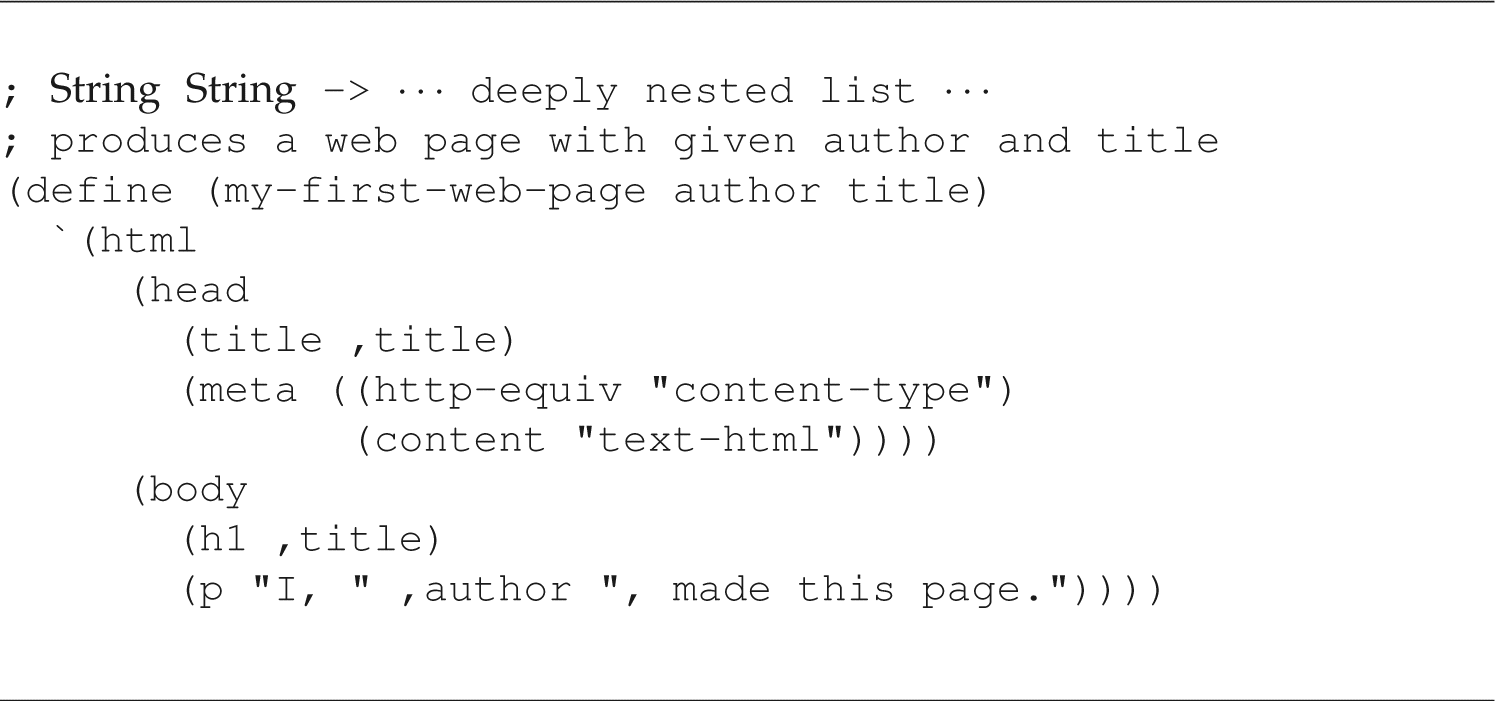
\includegraphics[width=0.85\textwidth]{images/00301.png}
  \caption{基于准引用与反引用的简易 HTML 页面生成器}
  \label{fig:html_generator}
\end{figure}

图~\ref{fig:nested_lists_webpage} 对比了该函数生成的嵌套列表与等价的标准 HTML 代码。

\begin{figure}[htbp]
  \centering
  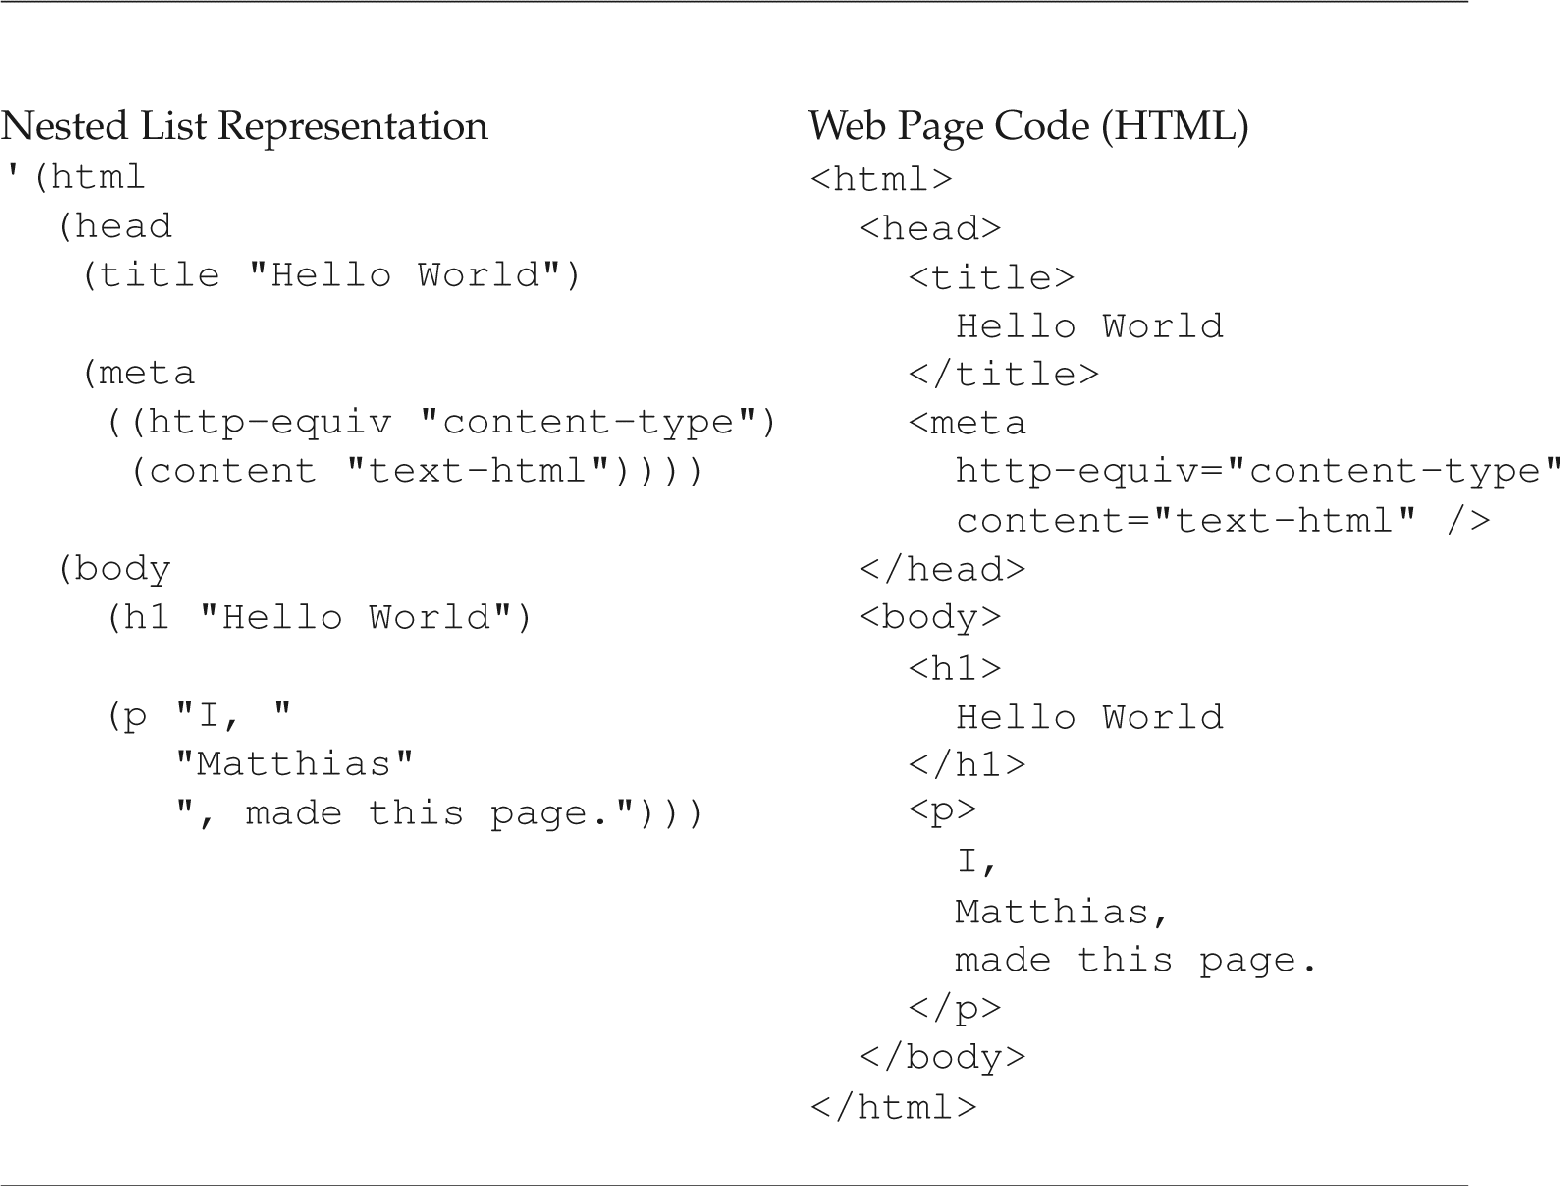
\includegraphics[width=0.85\textwidth]{images/00302.png}
  \caption{嵌套列表与对应生成的 HTML 网页源代码}
  \label{fig:nested_lists_webpage}
\end{figure}

\begin{exercise}{消除准引用与反引用}{232}
使用 \code{list} 消除下列各式中的反引号 \code{\`{}} 与逗号 \code{, }：
\begin{enumerate}
  \item \code{\`(1 "a" 2 \#false 3 "c")}
  \item 表格数据：
\begin{lstlisting}[language=BSL]
`(("alan" ,(* 2 500))
  ("barb" 2000)
  (,(string-append "carl" " , the great") 1500)
  ("dawn" 2300))
\end{lstlisting}
  \item 包含动态标题的网页结构。
\end{enumerate}
\end{exercise}

\intermezzosection{反引用拼接 (Unquote Splice)}

当子函数产生一个列表，而我们希望\textbf{将该子列表中的元素直接平铺、打散拼接到外层列表中}（而非作为一个独立的嵌套子列表）时，普通的反引用 \code{, } 就无法满足要求了：
\begin{replbox}
> `(tr ,(list "3" "4" "5"))
(list 'tr (list "3" "4" "5"))
\end{replbox}
而我们期望的结果往往是：
\begin{lstlisting}[language=BSL]
(list 'tr "3" "4" "5")
\end{lstlisting}

为此，BSL+ 提供了\term{反引用拼接}操作符 \code{,@}（unquote-splicing）：
\begin{replbox}
> `(tr ,@(list "3" "4" "5"))
(list 'tr "3" "4" "5")
\end{replbox}
它相当于把内层列表的外壳“剥开”，将其中的所有元素无缝融入外层列表！

利用 \code{,@}，我们可以极为优雅地编写函数生成任意行列尺寸的 HTML 表格：
\begin{lstlisting}[language=BSL]
; Number -> List
(define (make-cell n)
  `(td ,(number->string n)))

; List-of-numbers -> List
(define (make-row l)
  (cond
    [(empty? l) '()]
    [else (cons (make-cell (first l))
                (make-row (rest l)))]))

; List-of-numbers List-of-numbers -> List
(define (make-table row1 row2)
  `(table ((border "1"))
     (tr ,@(make-row row1))
     (tr ,@(make-row row2))))
\end{lstlisting}

\begin{exercise}{消除拼接简写}{233}
用 \code{list} 和 \code{cons} 重写包含 \code{,@} 的下列各式，并使用 \code{check-expect} 进行等价性检验：
\begin{enumerate}
  \item \code{\`(0 ,@'(1 2 3) 4)}
  \item 包含子列表拼接的表格行定义。
\end{enumerate}
\end{exercise}

\begin{exercise}{生成音乐排行榜网页 make-ranking}{234}
设计函数 \code{make-ranking}：消耗带有排名的歌曲名称列表，生成整齐美观的 HTML 网页表格展示（如图~\ref{fig:generated_webpage} 所示）。
\end{exercise}

\begin{figure}[htbp]
  \centering
  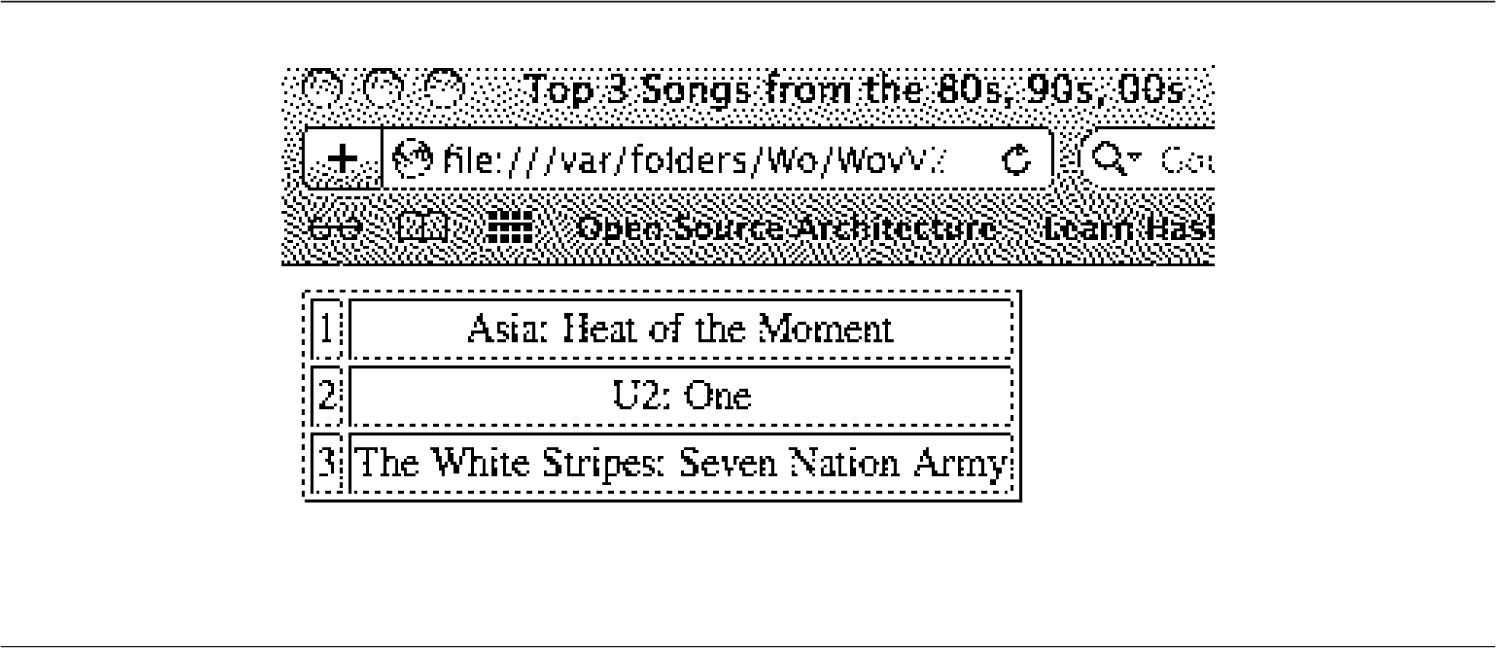
\includegraphics[width=0.75\textwidth]{images/00312.png}
  \caption{由 BSL+ 程序自动生成的动态网页效果}
  \label{fig:generated_webpage}
\end{figure}


% ==================== 第三部分：抽象 ====================
\part{抽象 (Abstraction)}
% ==============================================================================
% 第 14 章：处处皆相似 (Similarities Everywhere)
% ==============================================================================

\chapter{处处皆相似}
\label{sec:ch14_similarities}

如果你完成了第二部分中的（部分）练习，你会发现许多解法看起来惊人地相似。事实上，这种相似性可能会诱使你复制一个问题的解决方案，直接作为下一个问题的解答。但\term{切莫复制代码}，哪怕是你自己写的代码也不行。相反，你必须对相似的代码片段进行\term{抽象}（abstract）。本章将系统地教你如何进行抽象。

我们消除相似性的手段是特定于\term{中级学生语言}（Intermediate Student Language，简称 \term{ISL}）的。几乎所有其他主流编程语言都提供了类似的机制；在面向对象语言中，你还会发现额外的抽象机制。无论如何，这些机制都具有本章所阐述的基本特征，因此这里讲解的设计理念同样适用于其他各种计算语境。

\begin{notebox}[切换教学语言]
在 DrRacket 中，请从菜单栏的“Language”（语言）菜单中，选择“How to Design Programs”子菜单下的“Intermediate Student”（中级学生语言）。
\end{notebox}

% ------------------------------------------------------------------------------
\section{函数中的相似性}
\label{sec:14_1}

设计配方决定了函数的基本组织形式，因为模板是直接从数据定义中提炼出来的，完全不依赖于函数的具体目的。因此，处理同一种数据的函数看起来彼此相似也就不足为奇了。

请观察图~\ref{fig:86} 中的两个函数，它们都接收一个字符串列表并查找特定的字符串。左边的函数查找 \code{"dog"}，右边的函数查找 \code{"cat"}。这两个函数几乎毫无二致：每个函数都以字符串列表作为输入；每个函数体都由一个包含两个分支的 \code{cond} 表达式构成；当输入为空列表 \code{'()} 时，都产生 \code{\#false}；每个函数都使用 \code{or} 表达式来判断列表的首项是否为目标项，如果不是，则通过递归在列表的剩余部分中继续查找。唯一的区别在于嵌套表达式中用于比较的具体字符串：\code{contains-dog?} 使用了 \code{"dog"}，而 \code{contains-cat?} 使用了 \code{"cat"}。为了突出这些差异，图中对这两个字符串进行了阴影高亮。

\begin{figure}[htbp]
  \centering
  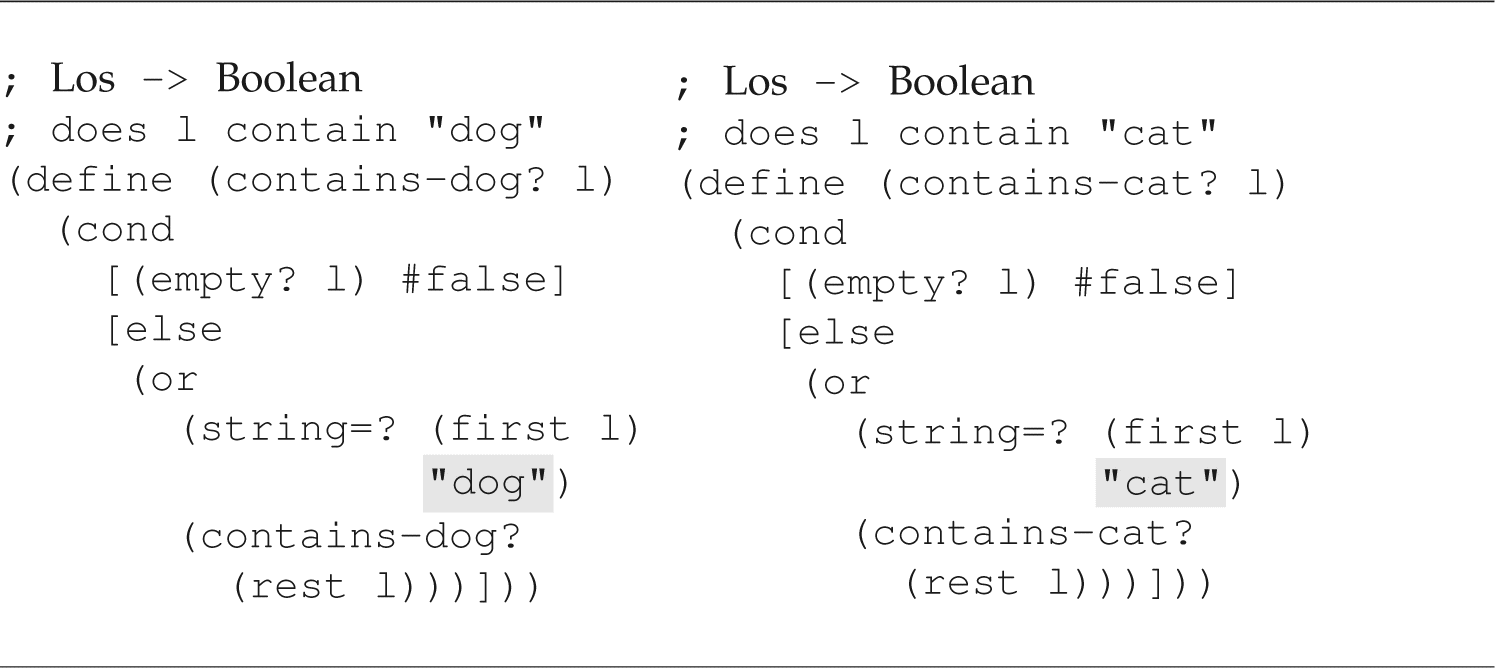
\includegraphics[width=0.85\textwidth]{images/00315.png}
  \caption{两个相似的函数}
  \label{fig:86}
\end{figure}

优秀的程序员往往“懒得”去定义好几个高度相近的函数。相反，他们会定义一个通用函数，既能在字符串列表中查找 \code{"dog"}，也能查找 \code{"cat"}。这个通用函数只需额外接收一项数据——即要查找的目标字符串——而在其他方面与原先的两个函数完全一致：

\begin{center}
  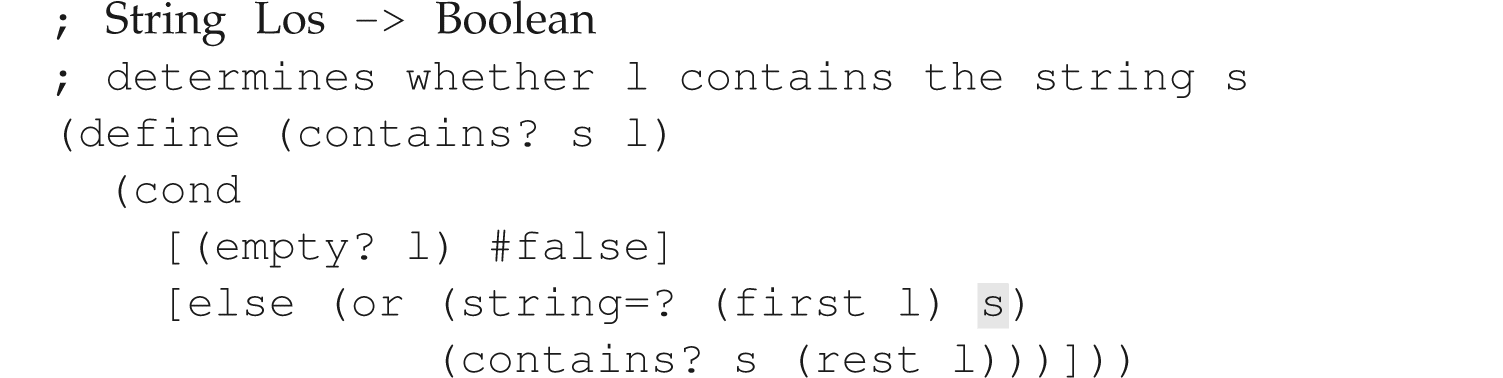
\includegraphics[width=0.85\textwidth]{images/00316.png}
\end{center}

如果你现在确实需要一个像 \code{contains-dog?} 这样的函数，只需将其定义为单行函数即可，对于 \code{contains-cat?} 也是如此。图~\ref{fig:87} 正是这么做的。你可以将它与图~\ref{fig:86} 进行简短对比，确保理解我们是如何从前者演进到后者的。最棒的是，有了 \code{contains?}，在字符串列表中查找任意字符串都变得轻而易举，我们再也不需要定义像 \code{contains-dog?} 这样专用的特殊函数了。

\begin{figure}[htbp]
  \centering
  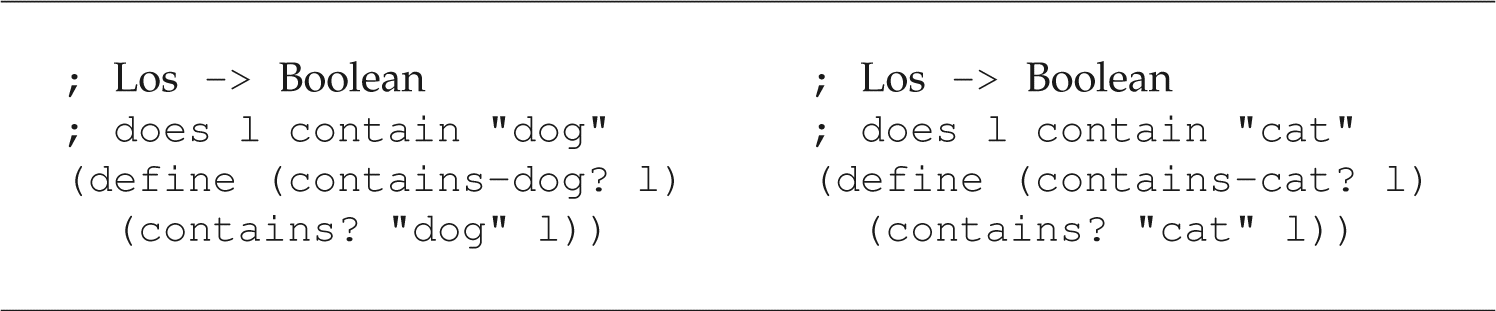
\includegraphics[width=0.85\textwidth]{images/00317.png}
  \caption{重新审视两个相似函数}
  \label{fig:87}
\end{figure}

你刚刚目睹的过程被称为\term{抽象}（abstraction），更准确地说，是\term{函数抽象}（functional abstraction）。对函数的不同版本进行抽象，是消除程序中重复与相似性的首要途径。正如你将看到的，消除相似性使得程序在长期维护中更容易保持稳健。

\begin{notebox}[“抽象”的数学来源]
计算机科学家从数学中借用了“抽象”这个术语。在数学中，“6”是一个抽象概念，因为它代表了对任意六个事物进行计数的所有方式。相比之下，“6 英寸”或“6 个鸡蛋”则是具体的使用形态。
\end{notebox}

\begin{exercise}{搜索单词}{235}
使用通用函数 \code{contains?}，分别定义在字符串列表中搜索 \code{"atom"}、\code{"basic"} 和 \code{"zoo"} 的函数。
\end{exercise}

\begin{exercise}{数字列表变换与抽象}{236}
为以下两个函数编写完整的测试套件：

\begin{center}
  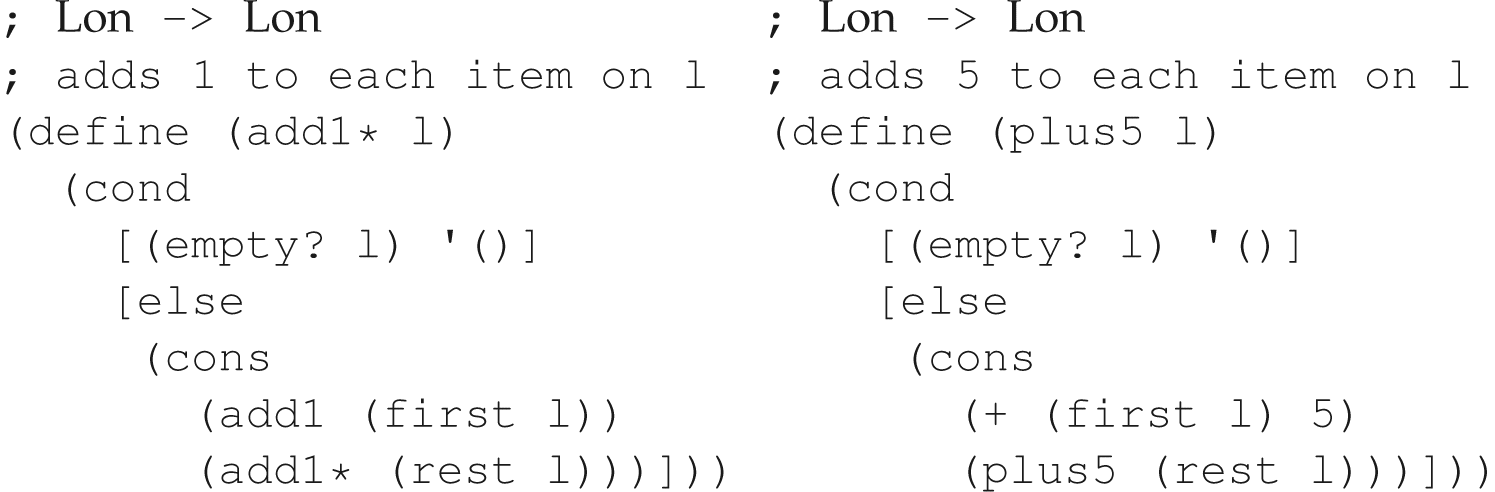
\includegraphics[width=0.85\textwidth]{images/00318.png}
\end{center}

然后对它们进行抽象。借助所提炼出的抽象函数，将上述两个函数重新定义为单行函数，并使用已有的测试套件确认修改后的定义能够正确工作。最后，再设计一个函数，从给定数字列表中的每个数字中减去 2。
\end{exercise}

% ------------------------------------------------------------------------------
\section{不同的相似性}
\label{sec:14_2}

在 \code{contains-dog?} 和 \code{contains-cat?} 的案例中，抽象看起来轻而易举。我们只需对比两个函数定义，用一个函数参数替换字面量字符串，并快速验证用抽象函数定义原函数十分容易即可。这种形式的抽象非常自然，以至于在本书的前两部分中已经多次自然而然地出现过。

本节将展示相同的原则如何衍生出一种更加强大的抽象形态。请看图~\ref{fig:88}。两个函数都接收一个数字列表和一个阈值。左边的函数产生列表中所有小于阈值的数字，而右边的函数则产生所有大于阈值的数字。

\begin{figure}[htbp]
  \centering
  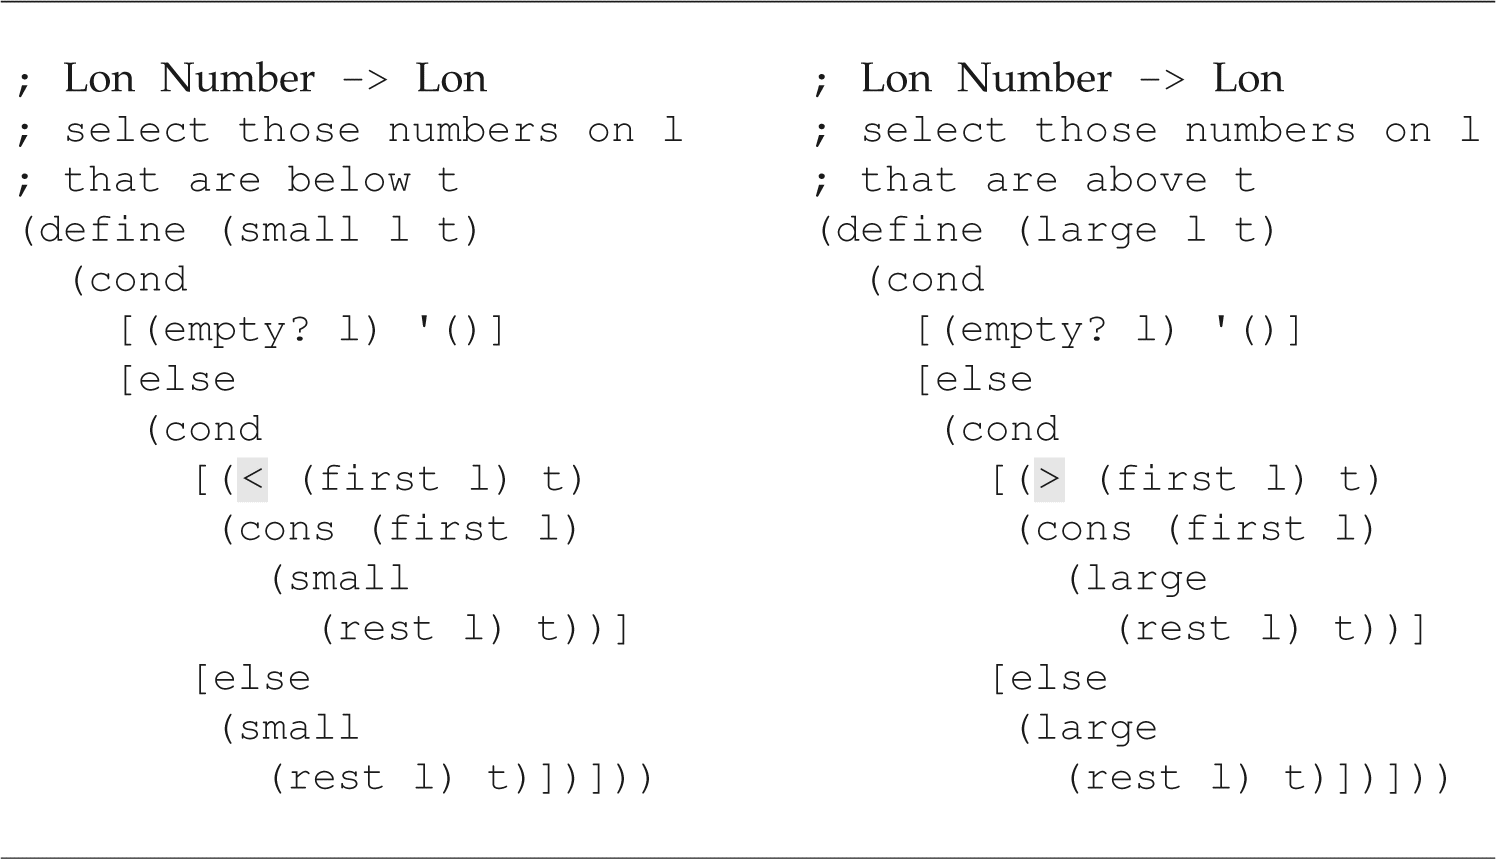
\includegraphics[width=0.85\textwidth]{images/00319.png}
  \caption{另外两个相似的函数}
  \label{fig:88}
\end{figure}

这两个函数仅在一处存在差异：用于决定列表中的数字是否应该包含在结果中的比较运算符。左边的函数使用了 \code{<}，右边的函数使用了 \code{>}。除此之外，除了函数名不同，两个函数在结构和逻辑上完全一模一样。

让我们遵循第一个示例的思路，引入一个额外的参数对这两个函数进行抽象。这一次，这个额外的参数所代表的不再是一个字符串，而是一个\term{比较运算符}：

\begin{center}
  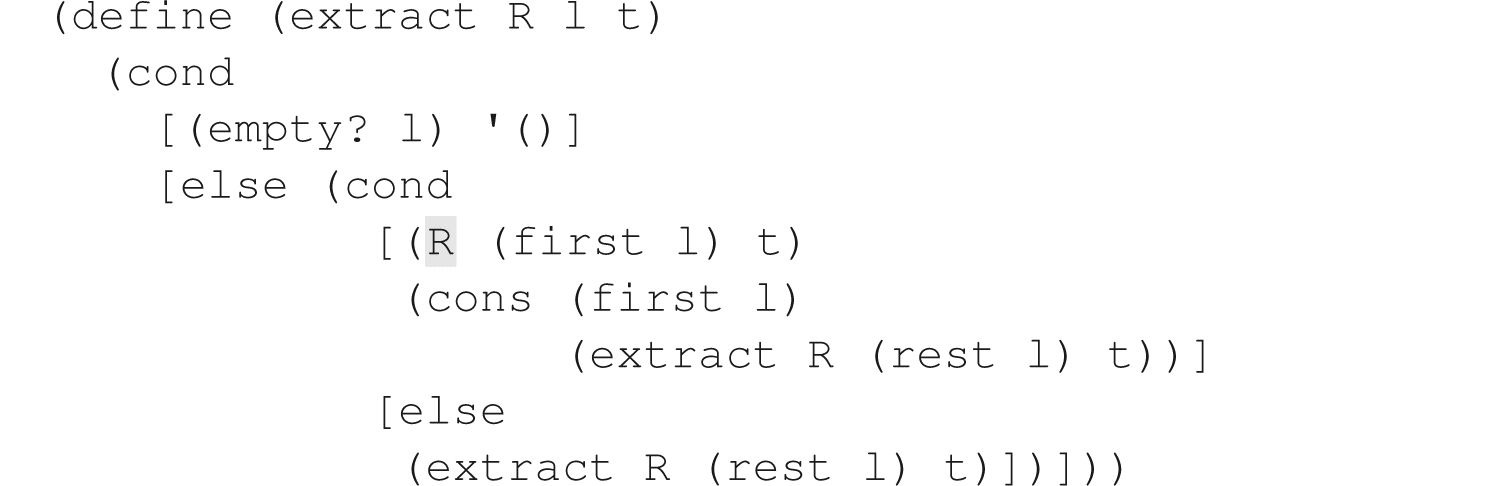
\includegraphics[width=0.85\textwidth]{images/00320.png}
\end{center}

要调用这个新函数，我们必须提供三个参数：一个比较两个数字的函数 \code{R}、一个数字列表 \code{l} 以及一个阈值 \code{t}。该函数随后会从 \code{l} 中提取出所有使得 \code{(R i t)} 求值为 \code{\#true} 的元素 \code{i}。

\begin{notebox}[驻足思考：函数作为参数！]
此时你应该停下来思考一下：这个定义真的合理吗？在没有任何多余仪式的情况下，我们竟然创建了一个\textbf{以函数作为参数的函数}——这可能是你以前从未见过的。然而事实证明，小巧简洁的教学语言 ISL 完全支持这类函数。而且，定义这种函数正是优秀程序员手中最强大的工具之一——即便在那些表面上似乎不直接支持高阶函数的语言中也是如此。
\end{notebox}

\begin{notebox}[微积分中的高阶函数]
如果你学过微积分，你一定遇到过微分算子和不定积分。它们本质上都是以函数作为输入并产生新函数的函数。不过，我们并不假设你学过微积分课程。
\end{notebox}

测试表明，\code{(extract < l t)} 的计算结果与 \code{(small l t)} 完全一致：

\begin{center}
  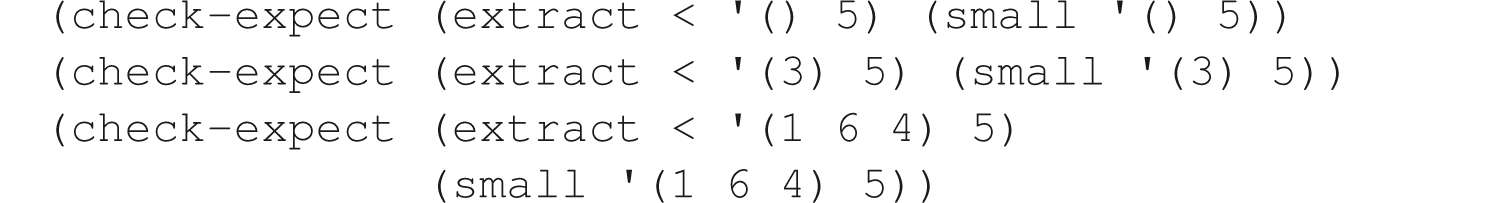
\includegraphics[width=0.85\textwidth]{images/00321.png}
\end{center}

类似地，\code{(extract > l t)} 产生与 \code{(large l t)} 相同的结果，这意味着你可以像这样重新定义原先的两个函数：

\begin{center}
  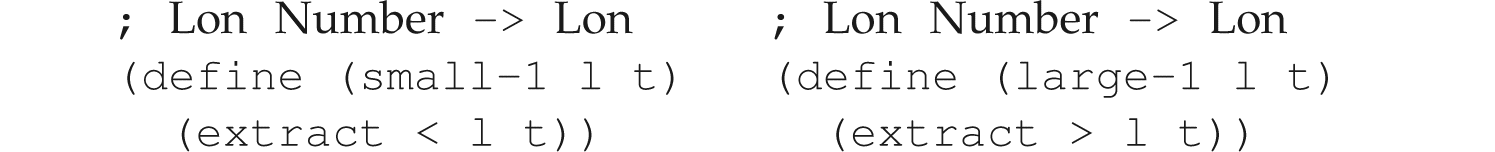
\includegraphics[width=0.85\textwidth]{images/00322.png}
\end{center}

这里最重要的领悟，并不仅仅在于 \code{small-1} 和 \code{large-1} 变成了单行定义。一旦拥有了像 \code{extract} 这样的抽象函数，你就可以将其广泛应用在其他场景中：

\begin{enumerate}
  \item \code{(extract = l t)}：提取出 \code{l} 中所有等于 \code{t} 的数字。
  \item \code{(extract <= l t)}：产生 \code{l} 中所有小于或等于 \code{t} 的数字列表。
  \item \code{(extract >= l t)}：计算出列表中所有大于或等于阈值的数字。
\end{enumerate}

事实上，传给 \code{extract} 的第一个参数根本不需要是 ISL 预定义的内置运算符。相反，你可以传入任何接收两个参数并返回布尔值的自定义函数。例如：

\begin{lstlisting}[language=BSL]
; Number Number -> Boolean
; 判断边长为 x 的正方形面积是否大于 c
(define (squared>? x c)
  (> (* x x) c))
\end{lstlisting}

也就是说，\code{squared>?} 检查命题 $x^2 > c$ 是否成立，它可以直接与 \code{extract} 配合使用：

\begin{lstlisting}[language=BSL]
(extract squared>? (list 3 4 5) 10)
\end{lstlisting}

这个调用将从 \code{(list 3 4 5)} 中提取出所有平方大于 10 的数字（即 4 和 5）。

\begin{exercise}{谓词求值}{237}
在 DrRacket 中求值 \code{(squared>? 3 10)} 与 \code{(squared>? 4 10)}。那么 \code{(squared>? 5 10)} 呢？
\end{exercise}

到目前为止，你已经看到抽象后的函数定义可以比原始函数有用得多。例如，\code{contains?} 比 \code{contains-dog?} 和 \code{contains-cat?} 更通用，而 \code{extract} 也比 \code{small} 和 \code{large} 更加强大。

抽象的另一个极其重要的优势在于：你现在为所有这些功能建立了\term{单点控制原则}（single point of control）。如果发现抽象函数中存在缺陷，只需修正其一处定义即可修复所有依赖于它的函数。同样，如果你找到了加速抽象函数计算或降低其能耗的优化方法，那么所有基于该函数定义的功能都将不费吹灰之力地享受到这些性能提升。接下来的练习将展示单点控制原则如何发挥效能。

\begin{notebox}[单点控制原则的普适价值]
抽象带来的这些好处存在于编程的各个层次：文字处理宏、电子表格公式、小型应用乃至大型工业级软件项目。为后者构建抽象正是驱动编程语言与软件工程前沿研究的核心动力。
\end{notebox}

\begin{exercise}{求最值函数的抽象与性能}{238}
将图~\ref{fig:89} 中的两个函数抽象为一个统一的通用函数。这两个函数都接收非空数字列表（Nelon）并返回一个数字。左边的函数求出列表中的最小值，右边的函数求出最大值。

\begin{center}
  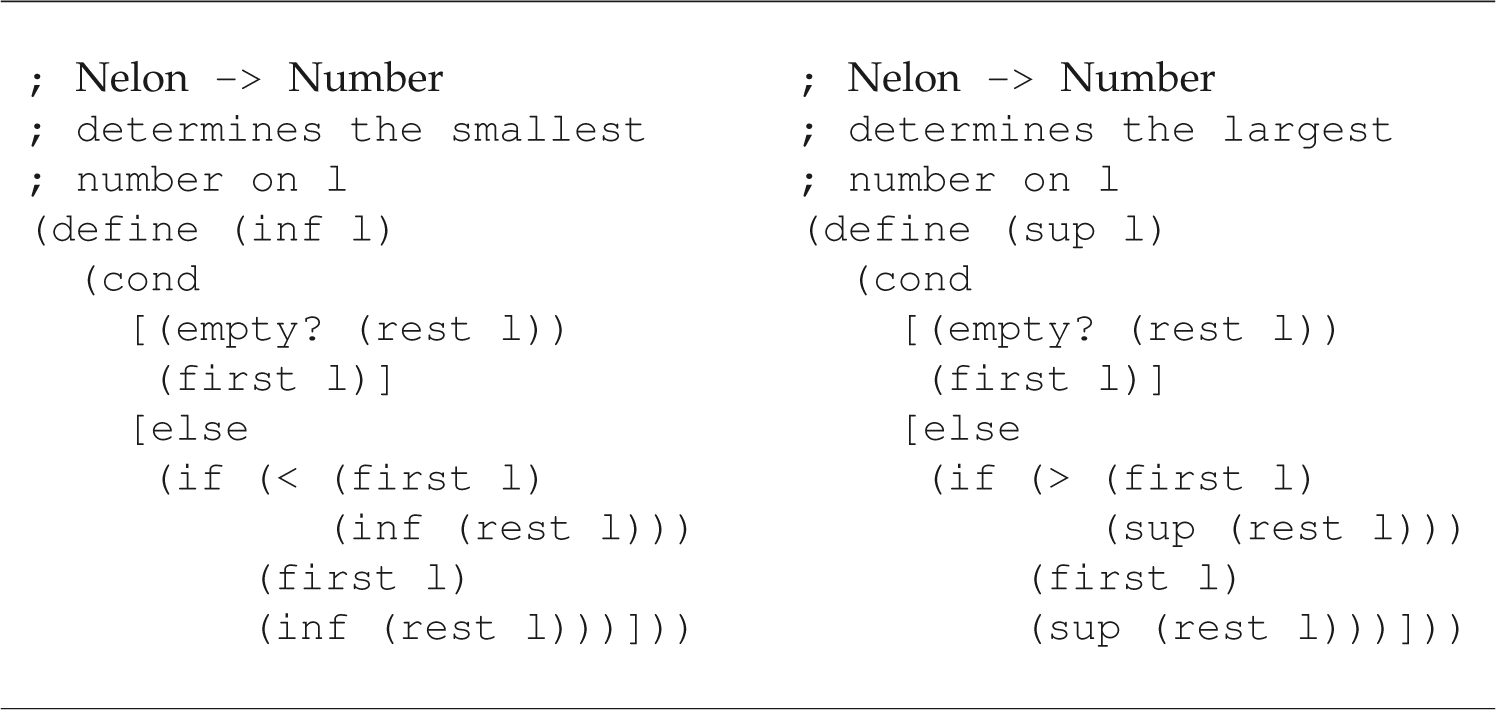
\includegraphics[width=0.85\textwidth]{images/00323.png}
  \captionof{figure}{在数字列表中查找下确界 (inf) 与上确界 (sup)}\label{fig:89}
\end{center}

借助该抽象函数定义 \code{inf-1} 与 \code{sup-1}。使用以下两个列表对它们进行测试：

\begin{center}
  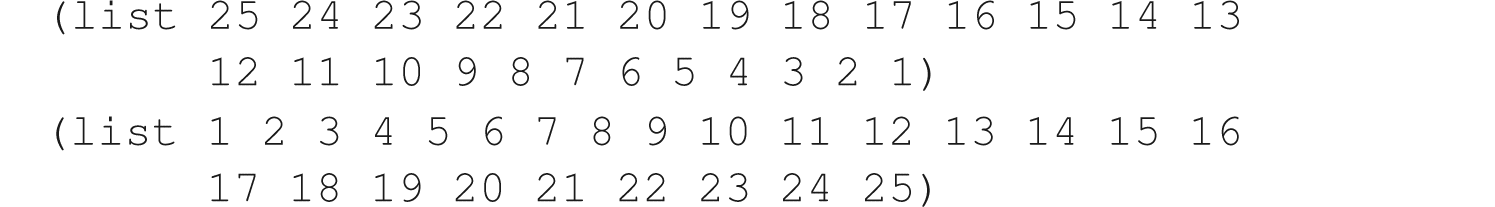
\includegraphics[width=0.85\textwidth]{images/00324.png}
\end{center}

为什么这些函数在处理某些长列表时会变得异常缓慢？

利用内置的 \code{max}（返回两个数中的较大者）和 \code{min}（返回较小者）重构原始函数。然后再次进行抽象，定义 \code{inf-2} 与 \code{sup-2}，并使用相同的测试输入重新测试。为什么这组新版本的运行速度会快得多？（关于此问题的另一种解答，请参见第 16.2 节）。
\end{exercise}

% ------------------------------------------------------------------------------
\section{数据定义中的相似性}
\label{sec:14_3}

现在请仔细观察以下两个数据定义：

\begin{center}
  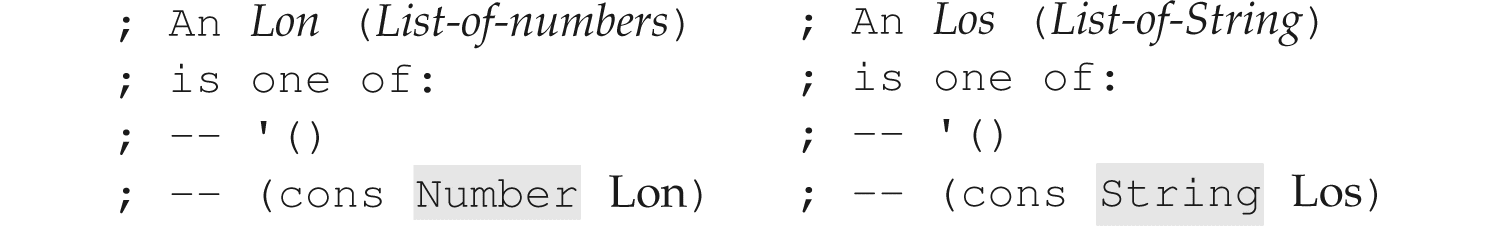
\includegraphics[width=0.85\textwidth]{images/00325.png}
\end{center}

左边定义了数字列表；右边描述了字符串列表。这两个数据定义极其相似。就像相似的函数一样，它们使用了两个不同的名称，但这无关紧要，因为换成任何名称都可以。唯一实质性的区别在于第二分支中 \code{cons} 内部的第一个位置，它规定了列表中包含哪种类型的元素。

为了消除这唯一的一处差异，我们把数据定义也当作函数来处理。我们引入一个参数，这使得数据定义看起来像一个函数；而在原先存在具体类型差异的地方，我们统一使用这个参数：

\begin{lstlisting}[language=BSL]
; A [List-of ITEM] is one of:
; -- '()
; -- (cons ITEM [List-of ITEM])
\end{lstlisting}

由于引入了参数，我们称这种抽象数据定义为\term{参数化数据定义}（parametric data definitions）。粗略地说，参数化数据定义抽象掉了对特定数据集合的直接引用，其方式与函数抽象掉特定具体值如出一辙。

核心问题当然是：这些参数的取值范围是什么？对于函数而言，形参代表一个未知的具体值；当函数被调用时，实参的具体值便确定下来。而对于参数化数据定义，形参代表\textbf{一整类值（数据集合）}。将某个数据集合的名称传递给参数化数据定义的过程被称为\term{实例化}（instantiation）。以下是抽象定义 \code{List-of} 的若干实例化示例：

\begin{itemize}
  \item 当我们写下 \code{[List-of Number]} 时，表示 \code{ITEM} 代表所有数字，因此它不过是 \code{List-of-numbers} 的另一个名字；
  \item 类似地，\code{[List-of String]} 与 \code{List-of-String} 定义了相同的数据类别；
  \item 如果我们定义了库存记录（Inventory Record）结构：
\begin{lstlisting}[language=BSL]
(define-struct ir [name price])
; An IR is a structure:
;   (make-ir String Number)
\end{lstlisting}
    那么 \code{[List-of IR]} 就是库存记录列表的类型名称。
\end{itemize}

按照惯例，我们在数据定义的形参中采用全大写字母（如 \code{ITEM}），而实参名称则按常规书写。

为了验证这些简写形式确实符合预期，我们可以用实际的数据定义名称（例如 \code{Number}）替换形参 \code{ITEM}，并为该数据定义赋予一个普通名称：

\begin{lstlisting}[language=BSL]
; A List-of-numbers-again is one of:
; -- '()
; -- (cons Number List-of-numbers-again)
\end{lstlisting}

由于数据定义是自引用的，我们替换了定义中的每一处参数。得到的结果与传统的数字列表定义完全相同，确实刻画了完全相同的数据类别。

让我们简要看看第二个例子，首先是一个结构体类型定义：

\begin{lstlisting}[language=BSL]
(define-struct point [hori veri])
\end{lstlisting}

以下是使用该结构体类型的两个不同数据定义：

\begin{center}
  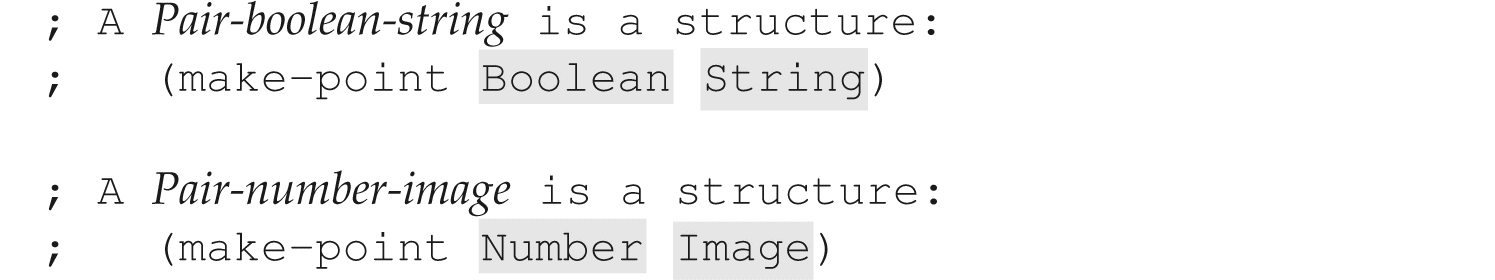
\includegraphics[width=0.85\textwidth]{images/00326.png}
\end{center}

在这种情况下，数据定义在两处存在差异（均以阴影标出）。\code{hori} 字段的差异彼此对应，\code{veri} 字段的差异亦是如此。因此，必须引入两个参数来构建抽象数据定义：

\begin{center}
  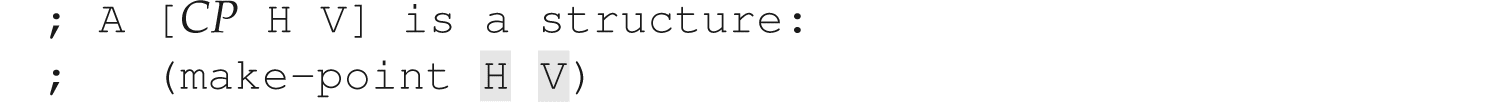
\includegraphics[width=0.85\textwidth]{images/00327.png}
\end{center}

这里 \code{H} 是用于 \code{hori} 字段数据集合的形参，而 \code{V} 则代表出现在 \code{veri} 字段中的数据集合。

要实例化一个带有两个参数的数据定义，你需要提供两个数据集合的名称。将 \code{Number} 和 \code{Image} 作为 \code{CP} 的参数，得到 \code{[CP Number Image]}，它描述了将数字与图像组合在一起的点；相比之下，\code{[CP Boolean String]} 则在点结构体中组合了布尔值与字符串。

\begin{exercise}{二元对的参数化数据定义}{239}
由两项构成的列表（二元对）是 ISL 编程中另一种频繁使用的数据形式。以下是带有两个参数的数据定义：

\begin{center}
  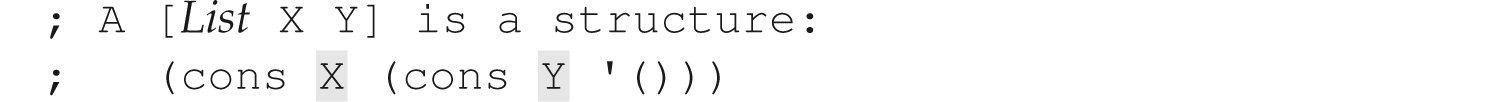
\includegraphics[width=0.85\textwidth]{images/00328.png}
\end{center}

实例化此定义以描述以下数据类别：
\begin{enumerate}
  \item 由两个 \code{Number} 构成的对；
  \item 由 \code{Number} 与 \code{1String} 构成的对；
  \item 由 \code{String} 与 \code{Boolean} 构成的对。
\end{enumerate}
并为这三种数据定义分别给出一个具体的实例。
\end{exercise}

一旦掌握了参数化数据定义，你就可以将它们组合嵌套使用，产生强大的表达效果。请看：

\begin{lstlisting}[language=BSL]
; [List-of [CP Boolean Image]]
\end{lstlisting}

最外层的标记是 \code{[List-of ...]}，这意味着你正在处理一个列表。至于列表中装的是什么样的数据，则需要观察其内部表达式：\code{[CP Boolean Image]} 将布尔值和图像组合在一个点中。因此，\code{[List-of [CP Boolean Image]]} 代表一个点列表，其中每个点都包含一个布尔值和一幅图像。类似地，\code{[CP Number [List-of Image]]} 则是 \code{CP} 的一种实例化，它将一个数字与一个图像列表组合在一起。

\begin{exercise}{嵌套结构的参数化抽象}{240}
以下是两个奇特但极其相似的数据定义：

\begin{center}
  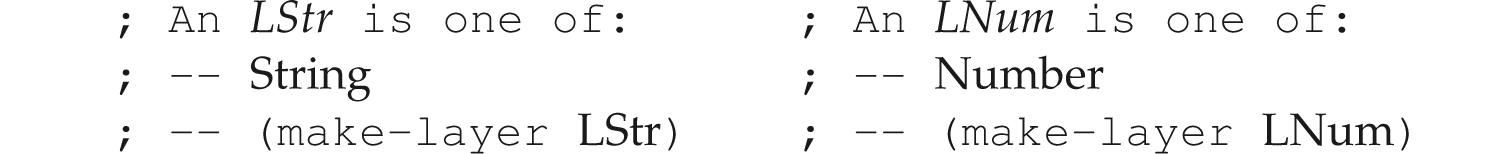
\includegraphics[width=0.85\textwidth]{images/00329.png}
\end{center}

这两个数据定义都依赖于以下结构体类型定义：

\begin{lstlisting}[language=BSL]
(define-struct layer [stuff])
\end{lstlisting}

两者都定义了嵌套形态的数据：一个是关于数字的，另一个是关于字符串的。请为两者各构造若干示例。对它们进行抽象，并展示如何通过实例化抽象定义还原出原先的两个具体定义。
\end{exercise}

\begin{exercise}{非空列表抽象}{241}
对比温度非空列表（\code{NEList-of-temperatures}）与布尔值非空列表（\code{NEList-of-Booleans}）的数据定义。然后提炼出一个通用的抽象参数化数据定义 \code{NEList-of}。
\end{exercise}

\begin{exercise}{Maybe 抽象与签名解读}{242}
以下是另一个常用的参数化数据定义：

\begin{lstlisting}[language=BSL]
; A [Maybe X] is one of:
; -- #false
; -- X
\end{lstlisting}

请解读下列数据定义的含义：\code{[Maybe String]}、\code{[Maybe [List-of String]]} 以及 \code{[List-of [Maybe String]]}。

此外，以下函数签名表达了什么含义？

\begin{center}
  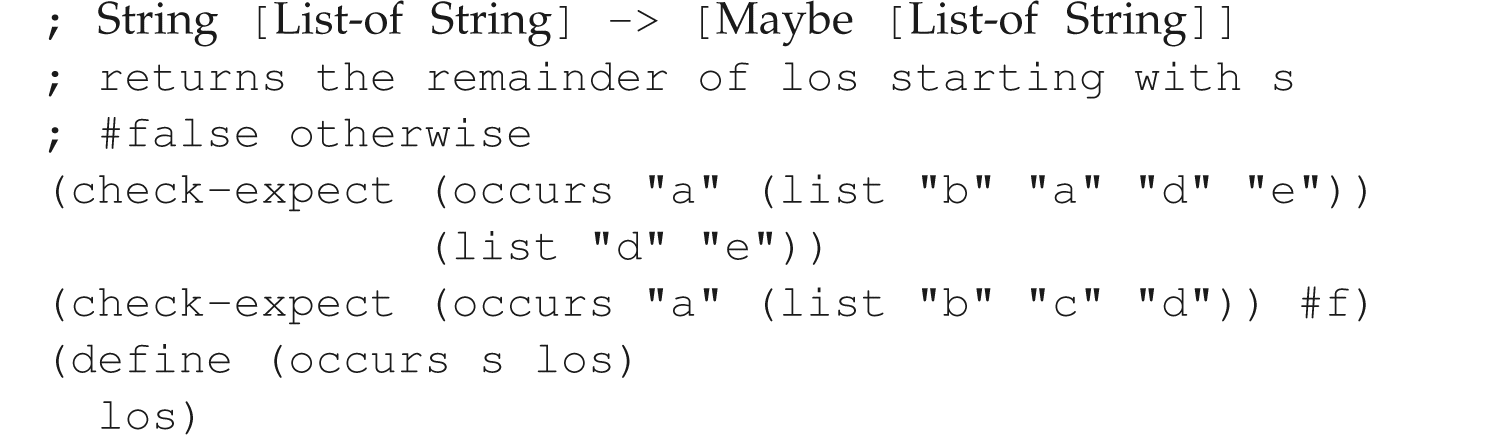
\includegraphics[width=0.85\textwidth]{images/00330.png}
\end{center}

请为其补全设计配方的其余步骤。
\end{exercise}

% ------------------------------------------------------------------------------
\section{函数即值}
\label{sec:14_4}

本部分所涉及的函数极大地拓展了我们对程序求值机制的理解。理解函数接收比数字更丰富的数据（例如字符串或图像）并不困难；结构体和列表虽然稍微复杂一些，但归根结底也是有限大小的“具体事物”。然而，\textbf{接收函数的函数}（以函数为参数的高阶函数）却显得十分奇特。事实上，这个想法在两个层面上打破了第一插曲中的语法规则：
\begin{enumerate}
  \item 原语和自定义函数的名字被作为实参传递给函数调用；
  \item 形参直接出现在函数调用表达式的首项（即函数名所在的位置）。
\end{enumerate}

明确了这个问题，就能看出 ISL 的语法与 BSL 究竟有何不同。首先，表达式语言必须允许函数名和内置原语名称像普通变量一样出现在参数位置。其次，在函数调用表达式的首项，除了固定的函数名和原语操作之外，必须允许出现形参和局部变量。

语法的这一放宽似乎要求对求值规则做出彻底变革，但实际上，我们只需要对\term{值的集合}（set of values）进行拓展：为了支持函数作为其他函数的参数，最根本的改变就是明确宣布：\term{函数与原语操作本身就是一等公民的值}（values）。

\begin{exercise}{辨识函数值}{243}
假设 DrRacket 的定义区中包含：

\begin{lstlisting}[language=BSL]
(define (f x) x)
\end{lstlisting}

判断以下表达式中哪些是\textbf{值}（values）：
\begin{enumerate}
  \item \code{(cons f '())}
  \item \code{(f f)}
  \item \code{(cons f (cons 10 (cons (f 10) '())))}
\end{enumerate}
请详细解释它们为什么是值，或者为什么不是值。
\end{exercise}

\begin{exercise}{合法表达式与文法放宽}{244}
论证为什么以下函数定义在 ISL 中是完全合法的：
\begin{enumerate}
  \item \code{(define (f x) (x 10))}
  \item \code{(define (f x) (x f))}
  \item \code{(define (f x y) (x 'a y 'b))}
\end{enumerate}
请给出你的推导与推理过程。
\end{exercise}

\begin{exercise}{函数相等性判断}{245}
开发一个名为 \code{function=at-1.2-3-and-5.775?} 的函数。给定两个从数字到数字的函数，该函数判断这两个函数在输入分别为 1.2、3 和 -5.775 时是否产生相同的结果。

数学家认为，如果两个函数在给定相同输入时总是计算出相同的结果——对于所有可能的输入皆如此——那么这两个函数就是相等的。

我们能否期望定义一个通用的 \code{function=?}，用于判定任意两个从数字到数字的函数是否在数学上严格相等？如果可以，请定义该函数；如果不可以，请解释原因，并思考这背后的深刻寓意：你遇到了第一个能够轻松用自然语言表述、却无法编写程序来判定的问题（不可判定性）。
\end{exercise}

% ------------------------------------------------------------------------------
\section{函数的求值计算}
\label{sec:14_5}

从 BSL+ 到 ISL 的转变，允许了将函数作为实参传递，并允许在函数调用表达式的首项使用变量名。DrRacket 处理这些位置上的名字与其他地方完全一样，只不过自然地期望其求值结果是一个函数。令人惊喜的是，代数中的经典\term{代换法则}（laws of substitution）稍作调整，就足以对 ISL 程序进行严格精确的求值推导。

让我们看看第 14.2 节中的 \code{extract} 函数是如何工作的。显而易见，以下等式成立：

\begin{lstlisting}[language=BSL]
(extract < '() 5) == '()
\end{lstlisting}

我们可以运用插曲 1 中的代换法则，继续在函数体内进行计算。与以往一样，形参 \code{R}、\code{l} 和 \code{t} 分别被实参 \code{<}、\code{'()} 和 \code{5} 代换。从这里开始，完全是朴素的算术与条件分支求值：

\begin{center}
  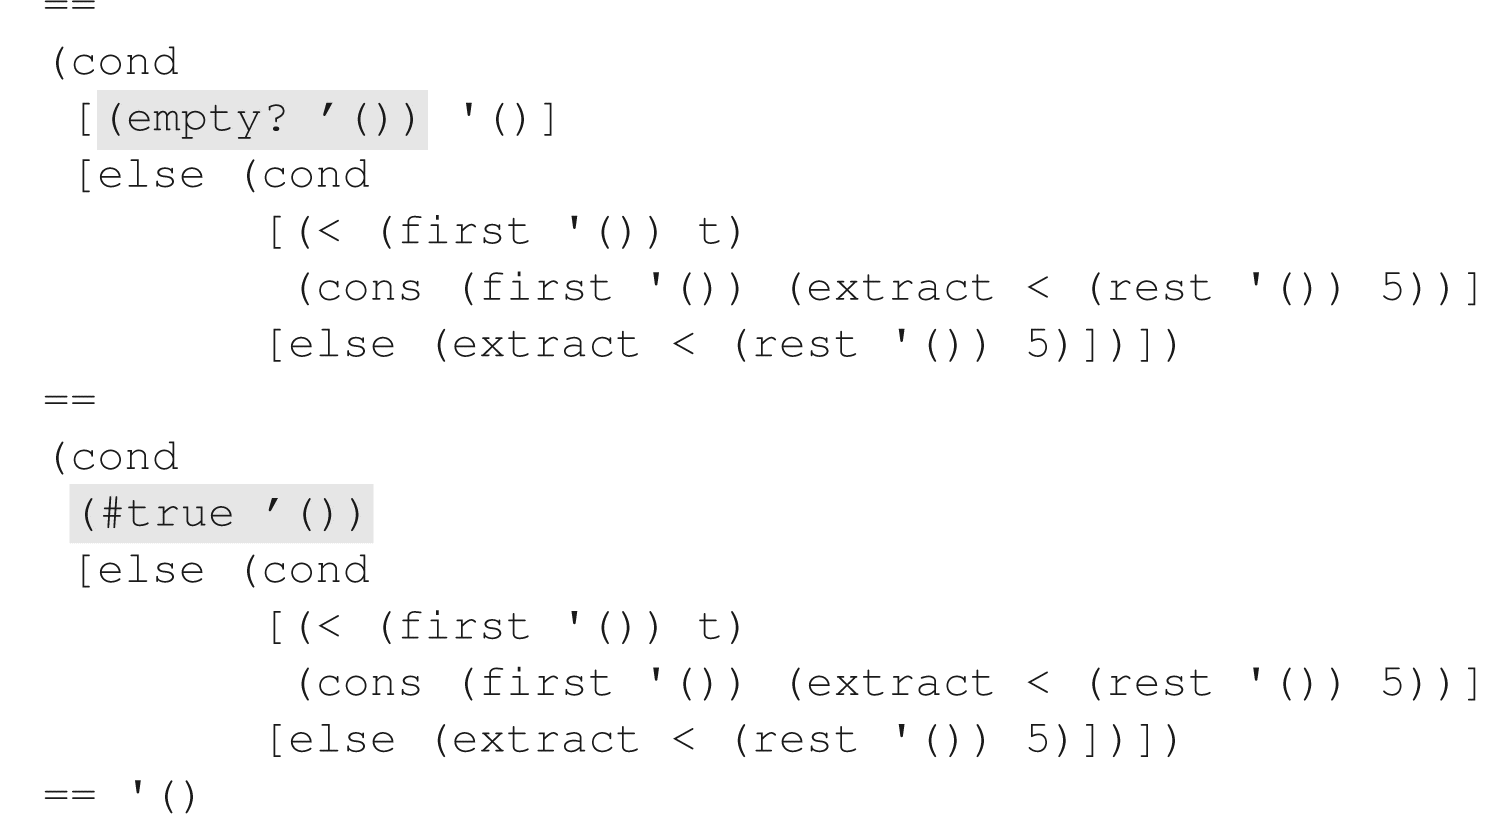
\includegraphics[width=0.85\textwidth]{images/00331.png}
\end{center}

接下来我们看一个包含单元素的列表：

\begin{lstlisting}[language=BSL]
(extract < (cons 4 '()) 5)
\end{lstlisting}

其结果应该是 \code{(cons 4 '())}，因为列表中唯一的元素是 4，且 \code{(< 4 5)} 为真。以下是单步求值的第一步：

\begin{center}
  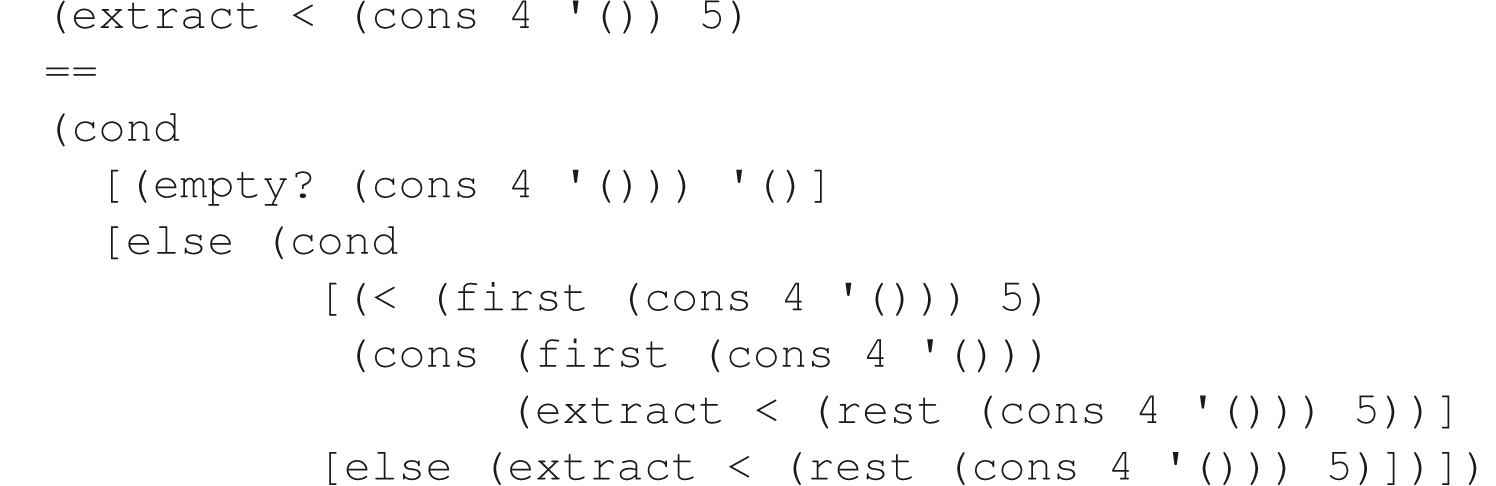
\includegraphics[width=0.85\textwidth]{images/00332.png}
\end{center}

同样，所有出现的 \code{R} 都被替换为 \code{<}，\code{l} 被替换为 \code{(cons 4 '())}，\code{t} 被替换为 \code{5}。接下来的计算直截了当：

\begin{center}
  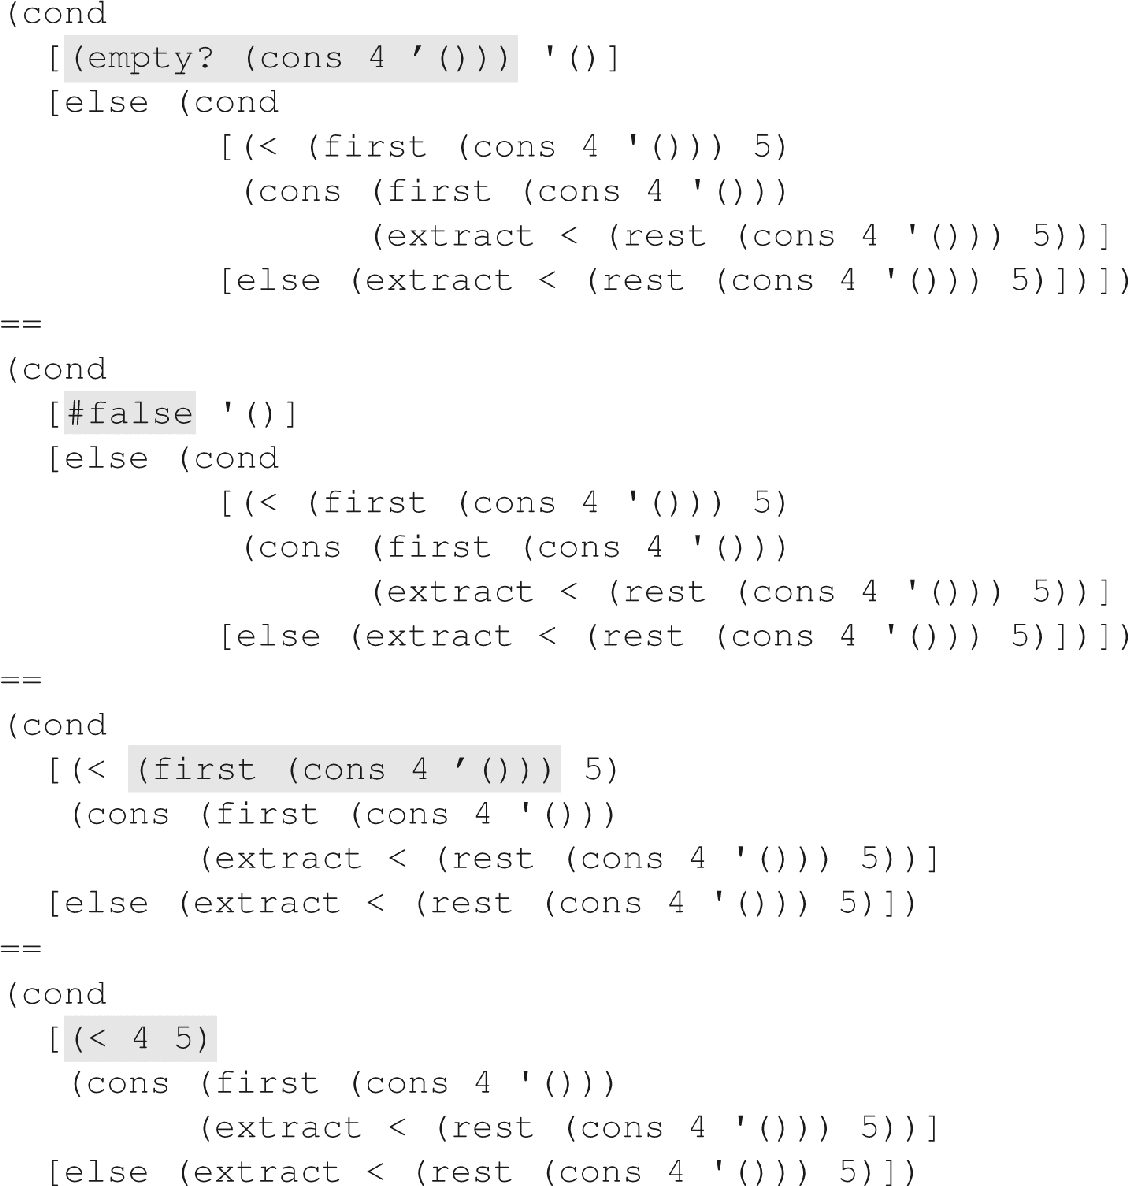
\includegraphics[width=0.85\textwidth]{images/00333.png}
\end{center}

这是最关键的一步：\code{<} 在被代换到函数调用首位后，作为普通的比较函数被直接应用。随后继续进行算术化简：

\begin{center}
  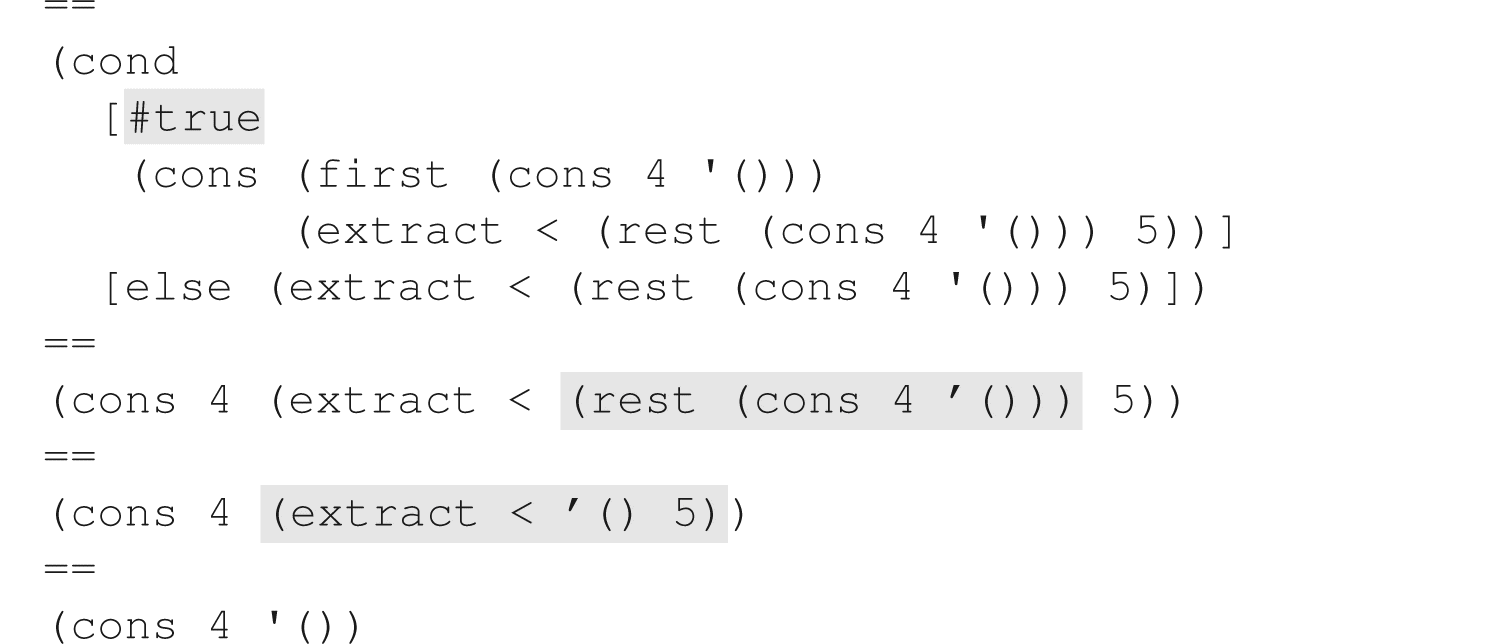
\includegraphics[width=0.85\textwidth]{images/00334.png}
\end{center}

最后一步正是上面已经证明过的等式，这意味着我们可以直接应用“等量代换”的代数公理。

我们的最后一个示例是将 \code{extract} 应用于一个包含两个元素的列表：

\begin{center}
  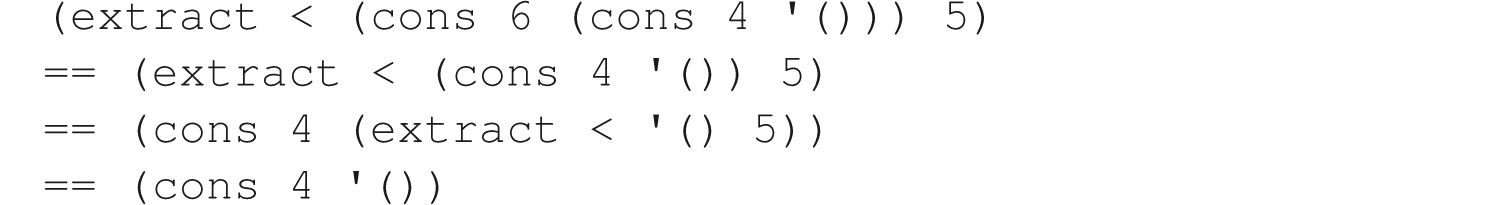
\includegraphics[width=0.85\textwidth]{images/00335.png}
\end{center}

其中的步骤 1 是全新的情形，它处理了当列表首项不小于阈值时，\code{extract} 如何将其剔除的情况。

\begin{exercise}{验证单步求值}{246}
使用 DrRacket 的单步求值器（Stepper），单步检验上一计算过程中的步骤 1：

\begin{center}
  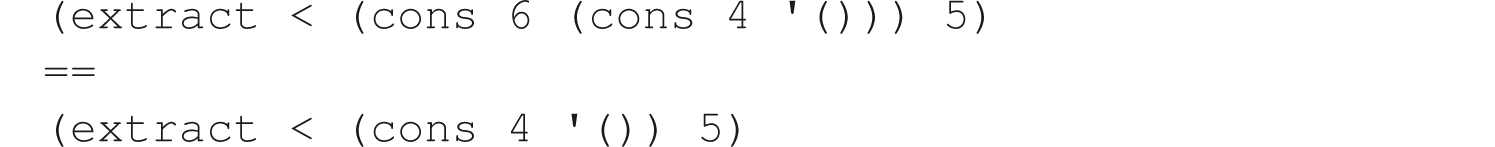
\includegraphics[width=0.85\textwidth]{images/00336.png}
\end{center}
\end{exercise}

\begin{exercise}{单步求值器跟踪 extract}{247}
使用 DrRacket 的单步求值器，完整跟踪并观察 \code{(extract < (cons 8 (cons 4 '())) 5)} 的求值全过程。
\end{exercise}

\begin{exercise}{高阶谓词的单步跟踪}{248}
在 DrRacket 单步求值器中跟踪求值 \code{(squared>? 3 10)} 和 \code{(squared>? 4 10)}。

请看以下交互会话：
\begin{replbox}
> (extract squared>? (list 3 4 5) 10)
(list 4 5)
\end{replbox}

以下是单步求值器展示的部分关键步骤：

\begin{center}
  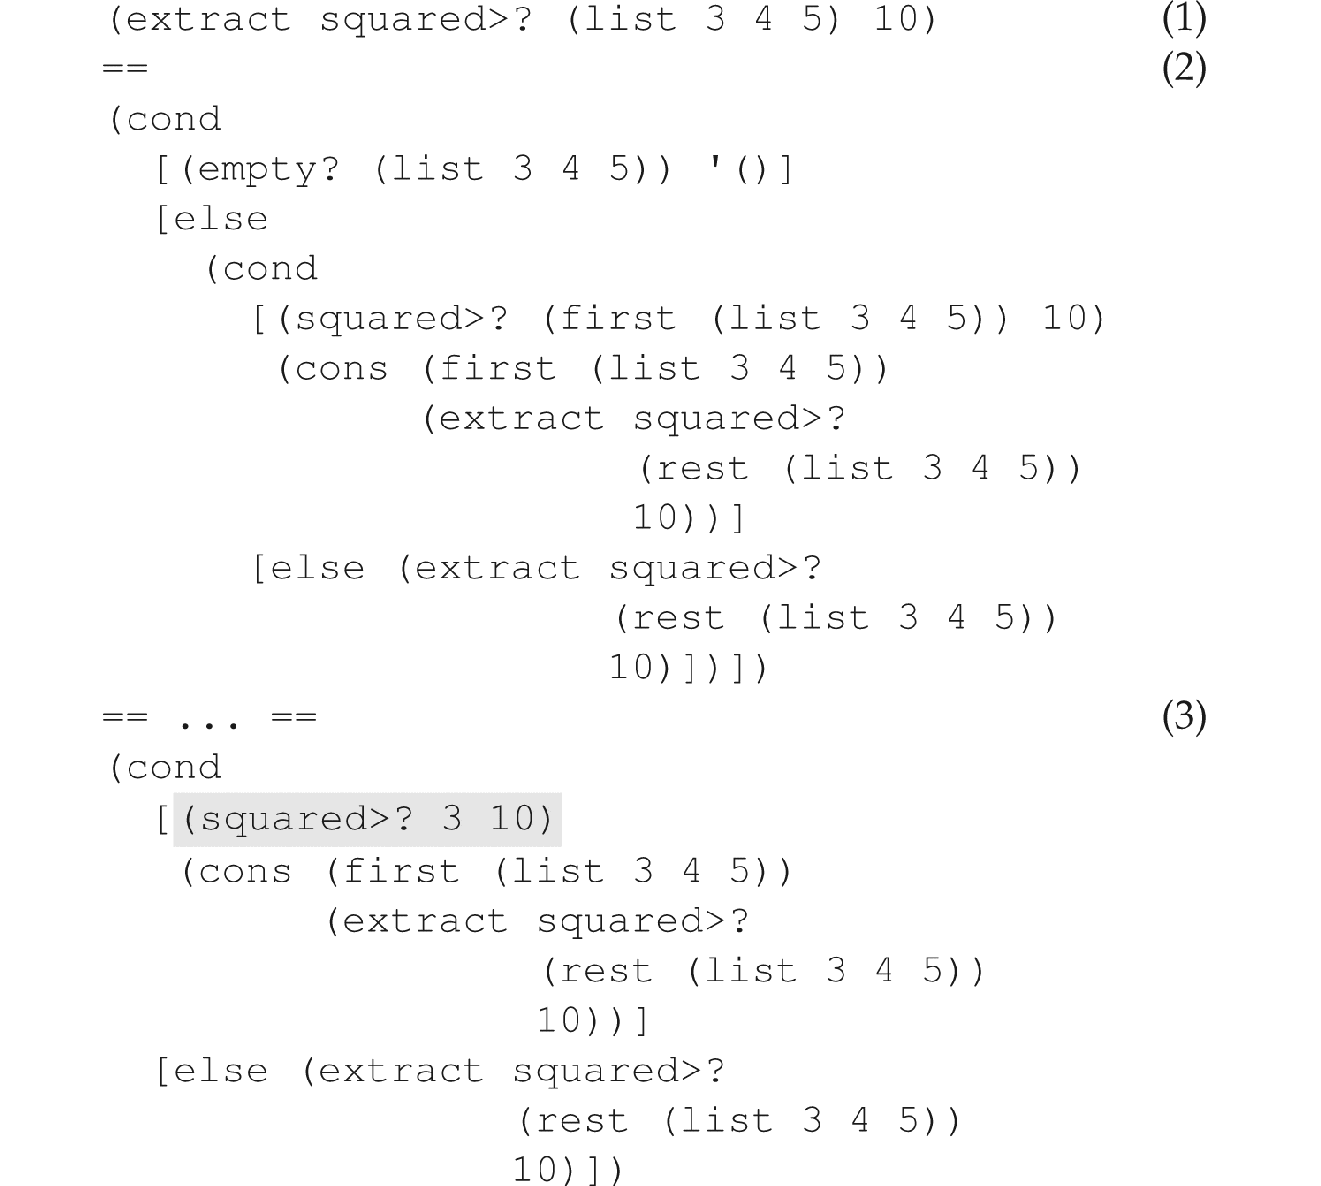
\includegraphics[width=0.85\textwidth]{images/00337.png}
\end{center}

使用单步求值器确认从第 (1) 步到第 (2) 步的推导。继续步进以填补第 (2) 步和第 (3) 步之间的细节空白。将每一步推导解释为代数法则的具体应用。
\end{exercise}

\begin{exercise}{作为值的函数求值过程}{249}
函数即值：可以作为实参、作为返回值、作为列表中的元素。将以下定义和表达式放置在 DrRacket 的定义窗口中，并使用单步求值器探究该程序的求值机制：

\begin{lstlisting}[language=BSL]
(define (f x) x)
(cons f '())
(f f)
(cons f (cons 10 (cons (f 10) '())))
\end{lstlisting}

单步求值器会将函数显示为 \code{lambda} 表达式；详见第 17 章。
\end{exercise}

% ==============================================================================
% 第 15 章：设计抽象 (Designing Abstractions)
% ==============================================================================

\chapter{设计抽象}
\label{sec:ch15_abstracting}

从本质上讲，\term{抽象}（abstract）就是将某些具体的事物转化为参数。在前一章中，我们已经多次见证了这一点：为了抽象相似的函数定义，我们引入新的参数来替换原定义中的具体值；为了抽象相似的数据定义，我们创建参数化数据定义。当你接触其他编程语言时，你也会发现它们的抽象机制同样要求引入参数，尽管形式上不一定表现为普通的函数形参。

% ------------------------------------------------------------------------------
\section{从示例中提炼抽象}
\label{sec:15_1}

当你最初学习加法时，你借助的是具体事例。父母可能教你掰着手指头去计算两个较小的数字相加；后来，你学会了如何将任意两个数字相加——此时你接触到了人生中的第一种抽象。再往后，你学会了列出方程式，将华氏温度与摄氏温度相互转换，或者根据车速和时间计算汽车行驶的距离。简而言之，你的认知过程始终是从非常具体的实例走向深刻的抽象关系。

本节将介绍一个系统的设计配方：\textbf{如何从具体示例中提炼抽象}。正如上一章所展示的，创建抽象本身并不复杂；我们把更具挑战性的部分留到下一节，在那里我们将学习如何寻找并复用已有的抽象。

回想一下第 14 章的核心精髓：我们从两个具体的定义出发，仔细对比它们，标出它们之间的差异，然后进行抽象。创建抽象的全部奥秘，基本上就在于此：

\begin{recipebox}{从示例中提炼函数抽象的设计配方}
\begin{enumerate}
  \item \textbf{步骤 1：对比相似项，标出差异}。当你发现两个函数定义除函数名与若干对应位置的具体值之外几乎完全一致时，将它们并排对比并标记出所有的不同之处。如果两处定义在多个位置存在差异，请用连线将相互对应的差异连接起来。
  \item \textbf{步骤 2：引入参数提炼抽象}。用全新的参数名称替换所标记的差异代码，并将这些形参添加到参数列表中。若有若干处差异相互对应，则使用同一个形参；不同维度的差异则引入不同的形参。
  \item \textbf{步骤 3：验证抽象的正确性}。借助新提炼出的抽象函数重新定义原先的两个具体函数，并使用它们原本的测试套件进行严格测试。
  \item \textbf{步骤 4：提炼抽象签名}。为抽象函数设计具有普适性的通用函数签名。
\end{enumerate}
\end{recipebox}

图~\ref{fig:90} 展示了一对相似的函数定义。这两个函数的作用都是将某种变换应用于列表中的每一个元素。它们唯一的本质区别在于：对列表中的元素具体应用了哪一个函数（图中以阴影高亮强调了这一本质差异）。除此之外，它们还存在两处非本质的差异：函数名称与列表形参的名称。

\begin{center}
  \begin{stepperbox}[unbreakable]
    \noindent\begin{minipage}[t]{0.48\linewidth}\vspace{0pt}
\begin{Verbatim}[commandchars=\\\{\}, fontsize=\fontsize{6.0pt}{7.2pt}\selectfont]
; List-of-numbers -> List-of-numbers
; converts a list of Celsius
; temperatures to Fahrenheit
(define (cf* l)
  (cond
    [(empty? l) '()]
    [else
      (cons
        (\hl{C2F} (first l))
        (cf* (rest l)))]))

; Number -> Number
; converts one Celsius
; temperature to Fahrenheit
(define (C2F c)
  (+ (* 9/5 c) 32))
\end{Verbatim}
    \end{minipage}\hfill
    \begin{minipage}[t]{0.48\linewidth}\vspace{0pt}
\begin{Verbatim}[commandchars=\\\{\}, fontsize=\fontsize{6.0pt}{7.2pt}\selectfont]
; Inventory -> List-of-strings
; extracts the names of
; toys from an inventory
(define (names i)
  (cond
    [(empty? i) '()]
    [else
      (cons
        (\hl{IR-name} (first i))
        (names (rest i)))]))

(define-struct IR
  [name price])
; An IR is a structure:
;   (make-IR String Number)
; An Inventory is one of:
; -- '()
; -- (cons IR Inventory)
\end{Verbatim}
    \end{minipage}
  \end{stepperbox}
  \captionof{figure}{一对相似的函数}\label{fig:90}
\end{center}

在步骤 2 中，我们用新参数 \code{g} 替换对应代码中的差异，得到如图~\ref{fig:91} 所示的一对函数。这一关键改动消除了本质差异：现在每个函数都遍历列表并将给定的函数参数 \code{g} 应用于每一项。

\begin{center}
  \begin{stepperbox}[unbreakable]
    \noindent\begin{minipage}[t]{0.48\linewidth}\vspace{0pt}
\begin{Verbatim}[commandchars=\\\{\}, fontsize=\fontsize{6.0pt}{7.2pt}\selectfont]
(define (cf* l \hl{g})
  (cond
    [(empty? l) '()]
    [else
      (cons
        (\hl{g} (first l))
        (cf* (rest l) g))]))

(define (map1 k g)
  (cond
    [(empty? k) '()]
    [else
      (cons
        (g (first k))
        (map1 (rest k) g))]))
\end{Verbatim}
    \end{minipage}\hfill
    \begin{minipage}[t]{0.48\linewidth}\vspace{0pt}
\begin{Verbatim}[commandchars=\\\{\}, fontsize=\fontsize{6.0pt}{7.2pt}\selectfont]
(define (names i \hl{g})
  (cond
    [(empty? i) '()]
    [else
      (cons
        (\hl{g} (first i))
        (names (rest i) g))]))

(define (map1 k g)
  (cond
    [(empty? k) '()]
    [else
      (cons
        (g (first k))
        (map1 (rest k) g))]))
\end{Verbatim}
    \end{minipage}
  \end{stepperbox}
  \captionof{figure}{抽象后的两个相似函数}\label{fig:91}
\end{center}

非本质差异（函数名与形参名）极易消除。如果你熟悉 DrRacket，就会知道利用其“Check Syntax”（语法检查）工具可以极其方便、系统地重命名变量。在图~\ref{fig:91} 底部，我们统一将抽象函数命名为 \code{map1}，并将列表形参命名为 \code{k}。无论你选取什么变量名，最终都会得到两个完全等价的函数定义。

我们的示例很纯粹。但在许多实际情况下，你会发现差异往往不止一对。关键在于找出差异之间的对应关系：在纸上标记差异时，用线将相关的差异方框连接起来，每一组相互对应的差异引入一个新形参。同时千万不要忘记：在函数的所有递归调用处，都要把这些新增的参数一同传递下去！

在步骤 3 中，我们必须验证新函数确实是原始函数对的正确抽象。验证意味着测试，而在此处测试意味着\textbf{用抽象函数重新定义原始函数}。

假设某个原始函数名为 \code{f-original} 并接收一个参数，而抽象函数名为 \code{abstract}。若 \code{f-original} 与另一个具体函数的区别在于使用了某个特定值 \code{val}，那么通过如下定义：

\begin{lstlisting}[language=BSL]
(define (f-from-abstract x)
  (abstract x val))
\end{lstlisting}

所引入的函数 \code{f-from-abstract} 在行为上应当与 \code{f-original} 完全等价。也就是说，对于任何合法输入值 \code{V}，\code{(f-from-abstract V)} 计算出的结果必须与 \code{(f-original V)} 毫无二致。特别地，原函数测试用例中的所有输入都必须满足这一点。因此，只需将原测试用例中的函数名修改为新函数并重新运行即可。

回到我们的主干示例：

\begin{lstlisting}[language=BSL]
; List-of-numbers -> List-of-numbers
(define (cf*-from-map1 l) (map1 l C2F))

; Inventory -> List-of-strings
(define (names-from-map1 i) (map1 i IR-name))
\end{lstlisting}

一个完整的程序必然附带测试。我们假设 \code{cf*} 和 \code{names} 本身就带有完备的测试：

\begin{lstlisting}[language=BSL]
(check-expect (cf* (list 100 0 -40))
              (list 212 32 -40))

(check-expect (names
                (list
                  (make-IR "doll" 21.0)
                  (make-IR "bear" 13.0)))
              (list "doll" "bear"))
\end{lstlisting}

为了确保通过 \code{map1} 定义的函数能够正确工作，只需复制测试并将函数名替换为新定义的函数：

\begin{lstlisting}[language=BSL]
(check-expect
  (cf*-from-map1 (list 100 0 -40))
                 (list 212 32 -40))

(check-expect
  (names-from-map1
    (list
      (make-IR "doll" 21.0)
      (make-IR "bear" 13.0)))
  (list "doll" "bear"))
\end{lstlisting}

在步骤 4 中，新的抽象需要一个签名。正如第 16 章将要阐述的，复用抽象正是从其签名开始的。为抽象函数寻找普适而有用的签名是一个极为严肃的问题。我们将在第 15.2 节中彻底解决这一问题。

一旦提炼出抽象函数，你就应该考查它是否还有其他广泛的用途。如果确实如此，该抽象就具备了极其可贵的复用价值。以 \code{map1} 为例，很容易看出如何使用它给数字列表中的每个数字加 1：

\begin{lstlisting}[language=BSL]
; List-of-numbers -> List-of-numbers
(define (add1-to-each l)
  (map1 l add1))
\end{lstlisting}

类似地，\code{map1} 也可以用来提取库存中每件商品的单价。当你能够为某个新抽象构想出众多应用场景时，就应当将其加入到工具函数库中。当然，往往前人早已想到了这一点，该函数很可能已经是编程语言标准库的一部分——对于 \code{map1} 而言，这正是后文将学到的内置 \code{map} 函数。

\begin{exercise}{设计 tabulate 抽象函数}{250}
设计函数 \code{tabulate}，它是图~\ref{fig:92} 中两个函数的抽象。当 \code{tabulate} 正确设计完成后，使用它来分别定义对平方函数 \code{sqr} 和正切函数 \code{tan} 进行表格制表的函数。

\begin{center}
  \begin{stepperbox}[unbreakable]
    \noindent\begin{minipage}[t]{0.48\linewidth}\vspace{0pt}
\begin{Verbatim}[commandchars=\\\{\}, fontsize=\fontsize{6.0pt}{7.2pt}\selectfont]
; Number -> [List-of Number]
; tabulates sin between n
; and 0 (incl.) in a list
(define (tab-sin n)
  (cond
    [(= n 0) (list (sin 0))]
    [else
      (cons
        (sin n)
        (tab-sin (sub1 n)))]))
\end{Verbatim}
    \end{minipage}\hfill
    \begin{minipage}[t]{0.48\linewidth}\vspace{0pt}
\begin{Verbatim}[commandchars=\\\{\}, fontsize=\fontsize{6.0pt}{7.2pt}\selectfont]
; Number -> [List-of Number]
; tabulates sqrt between n
; and 0 (incl.) in a list
(define (tab-sqrt n)
  (cond
    [(= n 0) (list (sqrt 0))]
    [else
      (cons
        (sqrt n)
        (tab-sqrt (sub1 n)))]))
\end{Verbatim}
    \end{minipage}
  \end{stepperbox}
  \captionof{figure}{练习 250 中的相似函数}\label{fig:92}
\end{center}
\end{exercise}

\begin{exercise}{设计 fold1 抽象函数}{251}
设计函数 \code{fold1}，它是图~\ref{fig:93} 中两个函数（求和 \code{sum} 与求积 \code{product}）的抽象。

\begin{center}
  \begin{stepperbox}[unbreakable]
    \noindent\begin{minipage}[t]{0.48\linewidth}\vspace{0pt}
\begin{Verbatim}[commandchars=\\\{\}, fontsize=\fontsize{6.0pt}{7.2pt}\selectfont]
; [List-of Number] -> Number
; computes the sum of
; the numbers on l
(define (sum l)
  (cond
    [(empty? l) 0]
    [else
      (+ (first l)
         (sum (rest l)))]))
\end{Verbatim}
    \end{minipage}\hfill
    \begin{minipage}[t]{0.48\linewidth}\vspace{0pt}
\begin{Verbatim}[commandchars=\\\{\}, fontsize=\fontsize{6.0pt}{7.2pt}\selectfont]
; [List-of Number] -> Number
; computes the product of
; the numbers on l
(define (product l)
  (cond
    [(empty? l) 1]
    [else
      (* (first l)
         (product (rest l)))]))
\end{Verbatim}
    \end{minipage}
  \end{stepperbox}
  \captionof{figure}{练习 251 中的相似函数}\label{fig:93}
\end{center}
\end{exercise}

\begin{exercise}{设计 fold2 抽象函数}{252}
设计函数 \code{fold2}，它是图~\ref{fig:94} 中两个函数的抽象。

\begin{center}
  \begin{stepperbox}[unbreakable]
    \noindent\begin{minipage}[t]{0.48\linewidth}\vspace{0pt}
\begin{Verbatim}[commandchars=\\\{\}, fontsize=\fontsize{6.0pt}{7.2pt}\selectfont]
; [List-of Number] -> Number
(define (product l)
  (cond
    [(empty? l) 1]
    [else
      (* (first l)
         (product
           (rest l)))]))
\end{Verbatim}
    \end{minipage}\hfill
    \begin{minipage}[t]{0.48\linewidth}\vspace{0pt}
\begin{Verbatim}[commandchars=\\\{\}, fontsize=\fontsize{6.0pt}{7.2pt}\selectfont]
; [List-of Posn] -> Image
(define (image* l)
  (cond
    [(empty? l) emt]
    [else
      (place-dot
        (first l)
        (image* (rest l)))]))

; Posn Image -> Image
(define (place-dot p img)
  (place-image
    dot
    (posn-x p) (posn-y p)
    img))

; graphical constants:
(define emt
  (empty-scene 100 100))
(define dot
  (circle 3 "solid" "red"))
\end{Verbatim}
    \end{minipage}
  \end{stepperbox}
  \captionof{figure}{练习 252 中的相似函数}\label{fig:94}
\end{center}

将本练习与练习 251 进行对比。尽管两者都涉及 \code{product} 函数，但本练习带来了额外的挑战，因为第二个函数 \code{image*} 接收的是 Posn 列表，而产生的结果却是一幅 Image 图像。然而，其解决方案完全在本节所学知识的射程之内。将本题的解答与上一题进行深入对比，将为下一节关于抽象签名的探索带来极其深刻的启发。
\end{exercise}

最后，当你处理数据定义时，抽象过程也是完全类似的：为数据定义添加的额外参数代表一类值集合，而测试则意味着为具体类型进行实例化。总体而言，抽象数据定义往往比抽象函数还要简单直观。

% ------------------------------------------------------------------------------
\section{签名中的相似性}
\label{sec:15_2}

事实证明，函数的\term{签名}（signature）是决定其能否被有效复用的关键所在。因此，你必须学会编写能够以最普适的形式描述抽象的通用签名。要理解这背后的原理，我们需要重新审视签名，并从一个简单却极其深刻的见解出发：\textbf{签名在本质上就是数据定义}。

签名与数据定义都用于界定一类数据集合；两者的区别在于数据定义给这类别赋予了名称，而签名往往直接匿名表达。然而，当你写下：

\begin{lstlisting}[language=BSL]
; Number Boolean -> String
(define (f n b) "hello world")
\end{lstlisting}

第一行描述了一整类数据，而第二行则声明 \code{f} 属于该类别。具体而言，该签名描述了“所有接收一个 Number 和一个 Boolean 并返回一个 String 的函数”所构成的集合。

总的来说，签名中的箭头记法与第 14.3 节中的 \code{List-of} 构造类似。\code{List-of} 接收一个数据集合（例如 \code{X}），描述所有由 \code{X} 构成的列表；而箭头记法接收任意数量的数据类别，描述由函数构成的集合。

这意味着：\textbf{抽象设计配方同样完全适用于签名}！你对比相似的签名，标出其中的差异，然后用参数替代它们。

让我们从 \code{cf*} 和 \code{names} 的签名对比开始：

\begin{center}
  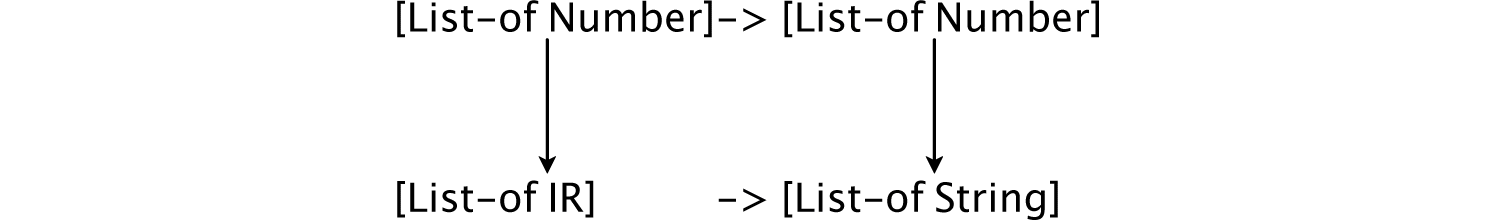
\includegraphics[width=0.85\textwidth]{images/00345.png}
\end{center}

对比两个签名显示它们在两处存在差异：在箭头左侧，是 \code{Number} 对比 \code{IR}；在箭头右侧，是 \code{Number} 对比 \code{String}。

如果我们用类型参数（例如 \code{X} 和 \code{Y}）替换这两处差异，就得到了统一的抽象签名：

\begin{lstlisting}[language=BSL]
; [X Y] [List-of X] -> [List-of Y]
\end{lstlisting}

新签名以方括号包裹的变量序列开头，这与函数形参列表及参数化数据定义形成了完美的类比。粗略地说，这些变量就是签名的\term{类型参数}（type parameters）。与参数化数据定义中的 \code{ITEM} 一样，\code{X} 和 \code{Y} 的取值范围是一整类具体的数据集合。

对该参数化签名的\term{实例化}，就是将其中的类型变量替换为具体的数据集合名称（或缩写）：
\begin{itemize}
  \item 若将 \code{X} 和 \code{Y} 同时替换为 \code{Number}，便还原出 \code{cf*} 的签名：
\begin{lstlisting}[language=BSL]
; [List-of Number] -> [List-of Number]
\end{lstlisting}
  \item 若将 \code{X} 替换为 \code{IR}，\code{Y} 替换为 \code{String}，便还原出 \code{names} 的签名：
\begin{lstlisting}[language=BSL]
; [List-of IR] -> [List-of String]
\end{lstlisting}
\end{itemize}
这充分解释了为什么我们可以将该参数化签名视为原始签名的抽象。

当我们为这两个函数引入额外的函数参数以构造 \code{map1} 时，它们的扩展签名如下所示：

\begin{center}
  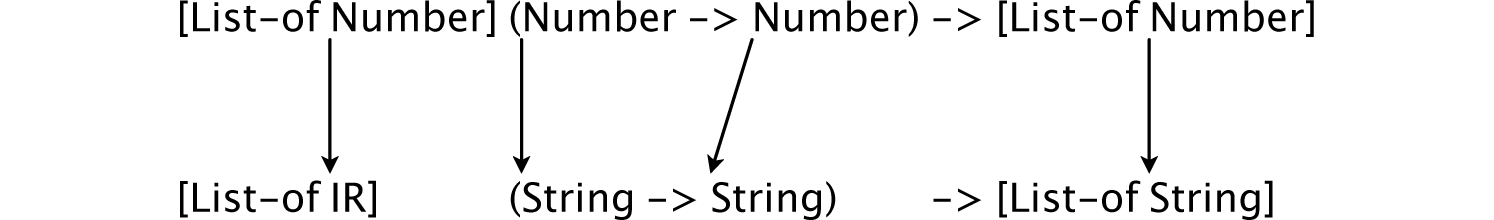
\includegraphics[width=0.85\textwidth]{images/00346.png}
\end{center}

连线标明了第二个参数（函数参数）内部的差异与原签名的差异紧密相关：新箭头左侧的 \code{Number} 与 \code{IR} 对应于首个列表参数中元素的类型；右侧的 \code{Number} 与 \code{String} 则对应于返回列表中元素的类型。

现在，我们应用同样的技巧，即可推导出 \code{map1} 的通用抽象签名：

\begin{lstlisting}[language=BSL]
; [X Y] [List-of X] [X -> Y] -> [List-of Y]
\end{lstlisting}

具体而言：\code{map1} 接收一个列表，其元素属于某种（尚待确定的）数据集合 \code{X}；它还接收一个能够将 \code{X} 类型的元素转换为另一类型 \code{Y} 的函数；最终，\code{map1} 产生一个包含 \code{Y} 类型元素的列表。

对签名进行抽象需要反复练习。让我们看第二个签名对：

\begin{lstlisting}[language=BSL]
; [List-of Number] -> Number
; [List-of Posn] -> Image
\end{lstlisting}

它们分别是练习 252 中 \code{product} 和 \code{image*} 的签名。结构对比表明：左侧签名中的第一个 \code{Number} 对应于右侧的 \code{Posn}，而第二个 \code{Number} 对应于右侧的 \code{Image}：

\begin{center}
  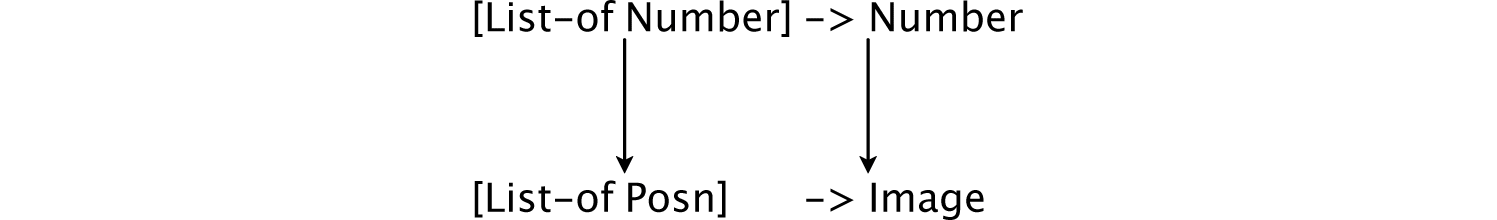
\includegraphics[width=0.85\textwidth]{images/00347.png}
\end{center}

为了提炼出二者的抽象签名，我们遵循设计配方的前两个步骤：

\begin{stepperbox}
  \noindent\begin{minipage}[t]{0.48\linewidth}\vspace{0pt}
\begin{Verbatim}[commandchars=\\\{\}, fontsize=\fontsize{6.0pt}{7.2pt}\selectfont]
(define (pr* l bs jn)
  (cond
    [(empty? l) bs]
    [else
      (jn (first l)
          (pr* (rest l)
               bs
               jn))]))
\end{Verbatim}
  \end{minipage}\hfill
  \begin{minipage}[t]{0.48\linewidth}\vspace{0pt}
\begin{Verbatim}[commandchars=\\\{\}, fontsize=\fontsize{6.0pt}{7.2pt}\selectfont]
(define (im* l bs jn)
  (cond
    [(empty? l) bs]
    [else
      (jn (first l)
          (im* (rest l)
               bs
               jn))]))
\end{Verbatim}
  \end{minipage}
\end{stepperbox}

由于两个函数在两组值上存在差异，修改后的版本额外接收两个参数：一个是基础情形下的基本值，另一个是用于将自然递归的结果与给定列表的首项进行结合的函数。

为这两个新函数写出带有具体参数的签名：对于 \code{pr*}：
\begin{lstlisting}[language=BSL]
; [List-of Number] Number [Number Number -> Number] -> Number
\end{lstlisting}
因为基础情形产生一个数字，且组合函数是 \code{+}。对于 \code{im*}：
\begin{lstlisting}[language=BSL]
; [List-of Posn] Image [Posn Image -> Image] -> Image
\end{lstlisting}
因为基础情形返回一幅图像，组合函数是 \code{place-dot}（将一个 Posn 和一幅 Image 组合为新 Image）。

将两者的结构对比扩展到包含新增输入的完整签名中：

\begin{center}
  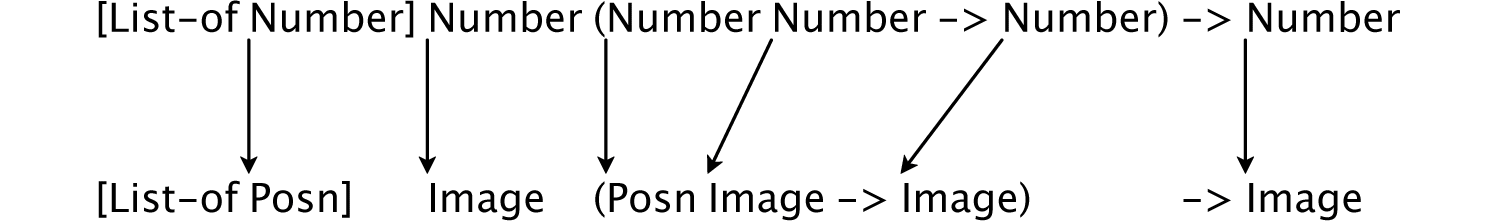
\includegraphics[width=0.85\textwidth]{images/00349.png}
\end{center}

这六对差异最终归结为两种本质对应：
\begin{enumerate}
  \item 部分 \code{Number} 对应于 \code{Posn}（由类型变量 \code{X} 表示）；
  \item 另一些 \code{Number} 对应于 \code{Image}（由类型变量 \code{Y} 表示）。
\end{enumerate}

由此，我们推导出了练习 252 中 \code{fold2} 抽象函数的普适签名：

\begin{lstlisting}[language=BSL]
; [X Y] [List-of X] Y [X Y -> Y] -> Y
\end{lstlisting}

\begin{notebox}[驻足验证类型实例化]
请务必停下来进行验证：将签名中的类型变量 \code{X} 与 \code{Y} 均替换为 \code{Number}，是否能够准确还原出 \code{pr*} 的签名？将它们分别替换为 \code{Posn} 和 \code{Image}，是否恰好得到 \code{im*} 的签名？
\end{notebox}

\begin{recipebox}{提炼抽象签名的系统步骤}
\begin{enumerate}
  \item \textbf{比较签名}：给定两个相似的函数定义 $f$ 与 $g$，对比它们的签名，标出相似的骨架与所有差异位置，并将相互对应的差异连线成对。
  \item \textbf{扩展签名}：为消除 $f$ 与 $g$ 的差异而引入抽象参数后，写出扩展后的中间签名。明确新增参数原本代表什么角色，以此确定新增参数的子签名。
  \item \textbf{引入类型参数}：检查步骤 1 中的对应分析是否依然适用于扩展签名。若适用，为每一类本质差异引入一个类型变量（如 \code{X}、\code{Y}）。当两个签名的表达式完全一致时，你就得到了通用的抽象签名。
  \item \textbf{检验与验证}：
    \begin{itemize}
      \item \textbf{代入检验}：通过对类型变量进行恰当的特化代入，必须能精确还原出各个具体函数的签名；
      \item \textbf{契约一致性}：检查通用签名与函数体代码是否完全吻合。若参数 $p$ 的签名为 \code{[A B -> C]}，则在代码中 $p$ 必须始终被传入两个参数（分别来自 $A$ 和 $B$），且调用 $p$ 的结果必须符合类型 $C$ 的上下文要求。
    \end{itemize}
\end{enumerate}
\end{recipebox}

\begin{exercise}{解读高阶函数签名}{253}
以下每个签名都描述了一类函数：
\begin{enumerate}
  \item \code{[Number -> Boolean]}
  \item \code{[Boolean String -> Boolean]}
  \item \code{[Number Number Number -> Number]}
  \item \code{[Number -> [List-of Number]]}
  \item \code{[[List-of Number] -> Boolean]}
\end{enumerate}
请用自然语言描述这些函数集合，并为每一类函数在 ISL 中给出至少一个具体的函数实例。
\end{exercise}

\begin{exercise}{排序函数的签名抽象}{254}
为以下两个函数分别拟定签名：
\begin{itemize}
  \item \code{sort-n}：接收一个数字列表和一个比较函数（该函数接收列表中的两个数字并返回布尔值），产生一个排好序的数字列表；
  \item \code{sort-s}：接收一个字符串列表和一个比较函数（该函数接收列表中的两个字符串并返回布尔值），产生一个排好序的字符串列表。
\end{itemize}
然后遵循上述配方对这两个签名进行抽象。并展示如何通过实例化该通用签名，来描述库存记录列表的排序函数 \code{sort-ir} 的签名。
\end{exercise}

\begin{exercise}{映射函数的签名抽象}{255}
为以下两个函数分别拟定签名：
\begin{itemize}
  \item \code{map-n}：接收一个数字列表和一个从数字到数字的函数，产生一个新的数字列表；
  \item \code{map-s}：接收一个字符串列表和一个从字符串到字符串的函数，产生一个新的字符串列表。
\end{itemize}
然后遵循上述步骤对这两个签名进行抽象。并展示如何将提炼出的通用签名实例化为前文 \code{map1} 函数的签名。
\end{exercise}

% ------------------------------------------------------------------------------
\section{单点控制原则}
\label{sec:15_3}

在广义上，编写程序就像撰写论文草稿。修改草稿对于纠正拼写错误、修饰语法漏洞、保持全书文风一致以及消除冗余重复至关重要。没有人愿意阅读充满大量重复段落的文章，更没有人愿意维护充斥着重复代码的软件系统。

消除代码中的相似性以提炼抽象具有不可估量的巨大优势：
\begin{itemize}
  \item 提炼抽象大幅简化了程序结构；
  \item 它能够暴露已有函数中潜藏的缺陷（尤其是当相似之处存在微妙偏差时）；
  \item \textbf{最为关键的优势在于：它为通用功能建立了统一的单点控制原则（Single Point of Control）}。
\end{itemize}

将某种功能的实现逻辑集中在单一位置，使得程序的长期维护变得轻而易举。当你发现一处缺陷时，只需修改一处代码即可彻底修复；当你需要让代码兼容新的数据形态时，只需在一个地方添加扩展；当你发现一种算法上的性能优化时，一次改动即可让系统中所有依赖该功能的地方同步受益。反之，如果你到处复制粘贴并微调代码，你就必须手动找到所有散落的副本逐一修改，否则旧错误将阴魂不散，或者只有某一个函数跑得飞快而其他地方依然缓慢。

\begin{notebox}[现代软件工程的核心准则]
\textbf{构建抽象，绝不复制粘贴并修改代码！} (Form an abstraction instead of copying and modifying any code.)
\end{notebox}

我们用于抽象函数的设计配方是构建抽象的最基础武器。掌握它需要大量的实战练习。随着熟练度的提升，你阅读、组织和维护复杂系统的能力将成倍跃升。最顶尖的程序员总是那些主动重构代码、积极提炼抽象、将相关逻辑收敛于单一控制源（单点控制原则）的工程师。在面向对象编程语言中，你还将接触到这一思想的另一种经典实现形态：基于类的继承与多态机制。

% ------------------------------------------------------------------------------
\section{从模板中提炼抽象}
\label{sec:15_4}

本部分的前两章展示了许多基于相同模板构建的函数。毕竟，设计配方的核心原则正是：\textbf{依据主要输入数据的组织结构来组织函数架构}。因此，处理同类数据的函数在外观与骨架上高度相近也就理所当然了。

事实上，我们甚至应当直接\textbf{对设计模板本身进行抽象}，而且这种抽象在理论上完全可以自动化完成（某些前沿的实验性编程语言已经做到了这一点）。尽管自动化推导仍是计算机科学的前沿研究课题，但你现在完全有能力理解其核心理念。

请观察我们熟悉的列表处理模板：

\begin{lstlisting}[language=BSL]
(define (fun-for-l l)
  (cond
    [(empty? l) ...]
    [else (... (first l) ...
               ... (fun-for-l (rest l)) ...)]))
\end{lstlisting}

该模板包含两个空白待填处，每个分支各有一个。当你利用此模板定义具体的列表处理函数时，你通常在第一个 \code{cond} 分支中填入一个具体的基准值，并在第二个分支中填入一个组合函数 \code{combine}。该 \code{combine} 函数接收列表的首项以及自然递归的结果，并将这两部分数据融合成最终的结果。

现在你已经掌握了如何创建抽象，完全可以从上述描述中直接定义出该模板的终极抽象函数——\code{reduce}：

\begin{lstlisting}[language=BSL, basicstyle=\scriptsize\ttfamily]
; [X Y] [List-of X] Y [X Y -> Y] -> Y
(define (reduce l base combine)
  (cond
    [(empty? l) base]
    [else (combine (first l)
                   (reduce (rest l) base combine))]))
\end{lstlisting}

它接收两个额外的实参：\code{base}（基准情形下的默认返回值）以及 \code{combine}（在第二分支中执行结果合并的二元函数）。

借助 \code{reduce}，你可以将绝大多数常规的列表处理函数直接写成优雅的“单行函数”。以下是求和 \code{sum} 与求积 \code{product} 的单行定义：

\begin{stepperbox}
  \noindent\begin{minipage}[t]{0.48\linewidth}\vspace{0pt}
\begin{Verbatim}[commandchars=\\\{\}, fontsize=\fontsize{6.0pt}{7.2pt}\selectfont]
; [List-of Number] -> Number
(define (sum lon)
  (reduce lon 0 +))
\end{Verbatim}
  \end{minipage}\hfill
  \begin{minipage}[t]{0.48\linewidth}\vspace{0pt}
\begin{Verbatim}[commandchars=\\\{\}, fontsize=\fontsize{6.0pt}{7.2pt}\selectfont]
; [List-of Number] -> Number
(define (product lon)
  (reduce lon 1 *))
\end{Verbatim}
  \end{minipage}
\end{stepperbox}

对于 \code{sum}，基础情形始终返回 0；而在第二分支中，通过 \code{+} 将首项与自然递归的结果相加。同样的推理完全解释了 \code{product}（基础情形返回 1，组合函数为 \code{*}）。几乎所有基础的列表处理函数，都可以通过这种方式用 \code{reduce} 简洁利落地定义出来！

% ==============================================================================
% 第 16 章：运用抽象 (Using Abstractions)
% ==============================================================================

\chapter{运用抽象}
\label{sec:ch16_using_abstractions}

一旦掌握了抽象，你就应当在一切可能的地方积极运用它们。抽象确立了\textbf{单点控制原则}，并且是极佳的省力工具。更确切地说，使用抽象能够极大帮助阅读代码的人理解你的意图。如果某个抽象广为人知、内置于语言核心或者来自标准库，那么相比于手写定制代码，它能够更加鲜明、清晰地传达该函数的核心职责。

本章全力聚焦于如何复用 ISL 中已有的丰富抽象。首先，我们将系统介绍 ISL 内置的经典抽象函数；接下来的各节则深入探讨复用这些抽象的具体技巧。其中的关键武器是一个全新的语法构造——\code{local}，它允许在函数内部就地定义局部变量、辅助函数甚至结构体类型。另一项辅助武器是第 17 章将正式引入的用于创建匿名函数的 \code{lambda} 构造。

% ------------------------------------------------------------------------------
\section{现有抽象}
\label{sec:16_1}

为了方便列表处理，ISL 内置提供了大量的经典抽象函数。图~\ref{fig:95} 和图~\ref{fig:96} 列出了其中最常用的若干核心函数及其权威签名：

\begin{figure}[htbp]
  \centering
\begin{lstlisting}[language=BSL, basicstyle=\scriptsize\ttfamily]
; [X] N [N -> X] -> [List-of X]
; constructs a list by applying f to 0, 1, ..., (sub1 n)
; (build-list n f) == (list (f 0) ... (f (- n 1)))
(define (build-list n f) ...)

; [X] [X -> Boolean] [List-of X] -> [List-of X]
; produces a list from those items on lx for which p holds
(define (filter p lx) ...)

; [X] [List-of X] [X X -> Boolean] -> [List-of X]
; produces a version of lx that is sorted according to cmp
(define (sort lx cmp) ...)

; [X Y] [X -> Y] [List-of X] -> [List-of Y]
; constructs a list by applying f to each item on lx
; (map f (list x-1 ... x-n)) == (list (f x-1) ... (f x-n))
(define (map f lx) ...)

; [X] [X -> Boolean] [List-of X] -> Boolean
; determines whether p holds for every item on lx
; (andmap p (list x-1 ... x-n)) == (and (p x-1) ... (p x-n))
(define (andmap p lx) ...)

; [X] [X -> Boolean] [List-of X] -> Boolean
; determines whether p holds for at least one item on lx
; (ormap p (list x-1 ... x-n)) == (or (p x-1) ... (p x-n))
(define (ormap p lx) ...)
\end{lstlisting}
  \caption{ISL 列表处理抽象函数 (1)}
  \label{fig:95}
\end{figure}

\begin{figure}[htbp]
  \centering
\begin{stepperbox}[unbreakable]
\begin{Verbatim}[commandchars=\\\{\}, fontsize=\scriptsize]
; [X Y] [X Y -> Y] Y [List-of X] -> Y
; applies f from right to left to each item in lx and b
; (foldr f b (list x-1 ... x-n)) == (f x-1 ... (f x-n b))
(define (foldr f b lx) ...)

(foldr + 0 '(1 2 3 4 5))
== (+ 1 (+ 2 (+ 3 (+ 4 \hl{(+ 5 0)}))))
== (+ 1 (+ 2 (+ 3 \hl{(+ 4 5)})))
== (+ 1 (+ 2 \hl{(+ 3 9)}))
== (+ 1 \hl{(+ 2 12)})
== (+ 1 14)

; [X Y] [X Y -> Y] Y [List-of X] -> Y
; applies f from left to right to each item in lx and b
; (foldl f b (list x-1 ... x-n)) == (f x-n ... (f x-1 b))
(define (foldl f b lx) ...)

(foldl + 0 '(1 2 3 4 5))
== (+ 5 (+ 4 (+ 3 (+ 2 \hl{(+ 1 0)}))))
== (+ 5 (+ 4 (+ 3 \hl{(+ 2 1)})))
== (+ 5 (+ 4 \hl{(+ 3 3)}))
== (+ 5 \hl{(+ 4 6)})
== \hl{(+ 5 10)}
\end{Verbatim}
\end{stepperbox}
  \caption{ISL 列表处理抽象函数 (2)}
  \label{fig:96}
\end{figure}

这些函数具有以下明确的行为约定：
\begin{itemize}
  \item \code{map}：将转换函数逐一应用到列表的每个元素上，收集并返回变换后的新列表；
  \item \code{filter}：提取列表中所有满足判定谓词的元素，剔除不满足条件的元素；
  \item \code{foldr}（右折叠）：从列表末尾开始，使用二元组合函数由右向左折叠列表，等价于结构型递归；
  \item \code{foldl}（左折叠）：从列表头部开始，使用二元组合函数由左向右依次累加处理；
  \item \code{build-list}：给定自然数 $n$ 与索引映射函数 $f$，构造列表 \code{(list (f 0) (f 1) ... (f (- n 1)))}；
  \item \code{andmap}：当且仅当列表中的\textbf{所有}元素都满足谓词时返回 \code{\#true}；
  \item \code{ormap}：只要列表中存在\textbf{至少一个}元素满足谓词便返回 \code{\#true}。
\end{itemize}

请注意标准库与我们在前文自定义抽象在参数顺序上的微妙区别：在标准库中，作为控制逻辑的函数参数通常放在首位（例如 \code{(map f l)} 而非 \code{(map1 l f)}），这使得高阶函数的意图一目了然。

\begin{figure}[htbp]
  \centering
\begin{lstlisting}[language=BSL, basicstyle=\scriptsize\ttfamily]
(define-struct address [first-name last-name street])
; An Addr is a structure:
;   (make-address String String String)
; interpretation associates an address with a person's name

; [List-of Addr] -> String
; creates a string from first names,
; sorted in alphabetical order,
; separated and surrounded by blank spaces
(define (listing l)
  (foldr string-append-with-space " "
         (sort (map address-first-name l) string<?)))

; String String -> String
; appends two strings, prefixes with " "
(define (string-append-with-space s t)
  (string-append " " s t))

(define ex0
  (list (make-address "Robert"   "Findler" "South")
        (make-address "Matthew"  "Flatt"   "Canyon")
        (make-address "Shriram"  "Krishna" "Yellow")))

(check-expect (listing ex0) " Matthew Robert Shriram ")
\end{lstlisting}
  \caption{借助抽象构建程序}
  \label{fig:97}
\end{figure}

\begin{exercise}{解读复杂的抽象函数}{256}
详细解释以下抽象函数的用途与运行机制：

\begin{lstlisting}[language=BSL]
; [X Y] [X Y -> Y] Y [List-of X] -> Y
; f*oldl works just like foldl
(check-expect (f*oldl cons '() '(a b c))
              (foldl cons '() '(a b c)))
(check-expect (f*oldl / 1 '(6 3 2))
              (foldl / 1 '(6 3 2)))
(define (f*oldl f e l)
  (foldr f e (reverse l)))
\end{lstlisting}

它的签名是什么？它可以用于解决哪些实际问题？
\end{exercise}

\begin{exercise}{手动设计 build-list 与 foldl}{257}
你可以凭借已学的设计配方手动设计 \code{build-list} 和 \code{foldl}，但它们与 ISL 的原生实现有所不同。例如，自行设计 \code{foldl} 函数通常需要借助列表反转函数 \code{reverse}。

请设计函数 \code{build-l*st}，其功能与 \code{build-list} 完全一致。（提示：回顾练习 193 中的 \code{add-at-end} 函数。注：第六部分将深入讲解从零开始设计这些函数所需的高级累加器概念）。
\end{exercise}

% ------------------------------------------------------------------------------
\section{局部定义}
\label{sec:16_2}

在许多情况下，传递给 \code{map}、\code{filter} 或 \code{foldr} 的辅助函数仅仅在某个特定函数的内部有意义。将这些辅助函数全部暴露在顶级全局命名空间中，不仅会污染命名空间，还会使代码的从属关系变得模糊混乱。

为此，ISL 提供了 \code{local} 表达式，其语法形式如下：

\begin{lstlisting}[language=BSL]
(local [definition ...] expression)
\end{lstlisting}

方括号内可以包含若干局部常量定义、结构体定义甚至函数定义；紧随其后的表达式则是 \code{local} 的主体，其求值结果即为整个 \code{local} 表达式的值。局部定义的名称仅在当前 \code{local} 表达式的范围（作用域）内可见。

\begin{figure}[htbp]
  \centering
\begin{lstlisting}[language=BSL, basicstyle=\scriptsize\ttfamily]
; [List-of Addr] -> String
; creates a string of first names,
; sorted in alphabetical order,
; separated and surrounded by blank spaces
(define (listing.v2 l)
  (local (; 1. extract names
          (define names  (map address-first-name l))
          ; 2. sort the names
          (define sorted (sort names string<?))
          ; 3. append them, add spaces
          ; String String -> String
          ; appends two strings, prefix with " "
          (define (helper s t)
            (string-append " " s t))
          (define concat+spaces
            (foldr helper " " sorted)))
    concat+spaces))
\end{lstlisting}
  \caption{利用 local 组织函数定义}
  \label{fig:98}
\end{figure}

图~\ref{fig:98} 展示了如何使用 \code{local} 将辅助函数私有化封装在主函数内部。图~\ref{fig:99} 则进一步展示了组织多个相互关联的函数定义。

\begin{figure}[htbp]
  \centering
\begin{lstlisting}[language=BSL, basicstyle=\scriptsize\ttfamily]
; [List-of Number] [Number Number -> Boolean]
; -> [List-of Number]
; produces a version of alon, sorted according to cmp
(define (sort-cmp alon0 cmp)
  (local (; [List-of Number] -> [List-of Number]
          ; produces the sorted version of alon
          (define (isort alon)
            (cond
              [(empty? alon) '()]
              [else
               (insert (first alon) (isort (rest alon)))]))

          ; Number [List-of Number] -> [List-of Number]
          ; inserts n into the sorted list of numbers alon
          (define (insert n alon)
            (cond
              [(empty? alon) (cons n '())]
              [else (if (cmp n (first alon))
                        (cons n alon)
                        (cons (first alon)
                              (insert n (rest alon))))])))
    (isort alon0)))
\end{lstlisting}
  \caption{利用 local 组织相互关联的函数定义}
  \label{fig:99}
\end{figure}

更重要的是，\code{local} 不仅提升了模块化与可读性，还能带来戏剧性的\textbf{计算性能提升}！

回顾第 14.2 节的练习 238，那里的 \code{inf} 和 \code{sup} 函数在处理长列表时性能极差，其根源在于：在条件分支中，递归调用被重复执行了两次。图~\ref{fig:100} 展示了如何使用 \code{local} 将递归结果绑定到一个局部变量中，从而避免指数级的冗余计算，将算法的时间复杂度从 $O(2^n)$ 骤降为线性时间 $O(n)$！

\begin{figure}[htbp]
  \centering
\begin{stepperbox}[unbreakable]
\begin{Verbatim}[commandchars=\\\{\}, fontsize=\scriptsize]
; Nelon -> Number
; determines the smallest number on l
(define (inf.v2 l)
  (cond
    [(empty? (rest l)) (first l)]
    [else
     (local (\hl{(define smallest-in-rest (inf.v2 (rest l)))})
       (if (< (first l) smallest-in-rest)
           (first l)
           smallest-in-rest))]))
\end{Verbatim}
\end{stepperbox}
  \caption{使用 local 显著提升计算性能}
  \label{fig:100}
\end{figure}

\begin{exercise}{重构多边形绘制函数}{258}
使用 \code{local} 表达式重构第 11.3 节（图~\ref{fig:drawing_polygon}）中用于绘制多边形的函数集。如果某个全局函数在很多不同场景下都普遍有用，请保留为全局定义；仅将专用的辅助函数局部化。
\end{exercise}

\begin{exercise}{重构单词重排程序}{259}
使用 \code{local} 表达式整理第 12.4 节中用于重排单词字母的函数。
\end{exercise}

\begin{exercise}{验证 inf.v2 的性能飞跃}{260}
通过重复练习 238 中的性能对比实验，在 DrRacket 中亲手验证图~\ref{fig:100} 中 \code{inf.v2} 的运行速度提升。
\end{exercise}

\begin{exercise}{库存函数性能优化}{261}
请观察图~\ref{fig:101} 中的库存处理函数。在嵌套的 \code{cond} 表达式中，两个分支都重复计算了 \code{(extract1 (rest an-inv))}。使用 \code{local} 为该公共表达式命名。这种优化是否能显著提升程序的运行速度？为什么？

\begin{stepperbox}
\begin{Verbatim}[commandchars=\\\{\}, fontsize=\scriptsize]
; Inventory -> Inventory
; creates an Inventory from an-inv for all
; those items that cost less than a dollar
(define (extract1 an-inv)
  (cond
    [(empty? an-inv) '()]
    [else
     (cond
       [(<= (ir-price (first an-inv)) 1.0)
        (cons (first an-inv) \hl{(extract1 (rest an-inv))})]
       [else \hl{(extract1 (rest an-inv))}])]))
\end{Verbatim}
\end{stepperbox}
\captionof{figure}{在库存记录中查找（参见练习 261）}\label{fig:101}
\end{exercise}

% ------------------------------------------------------------------------------
\section{局部定义增强表达力}
\label{sec:16_3}

\code{local} 最震撼人心的能力，在于它极大地增强了语言的\term{表达力}（expressive power）。

在 \code{local} 内部定义的函数，不仅可以访问自己的形参，还可以自由访问\textbf{外层外围函数的所有参数和常量}。这正是计算机科学中著名的\term{闭包}（closure）概念的雏形！

\begin{figure}[htbp]
  \centering
\begin{lstlisting}[language=BSL, basicstyle=\scriptsize\ttfamily]
; FSM FSM-State -> FSM-State
; matches the keys pressed by a player with the given FSM
(define (simulate fsm s0)
  (local (; State of the World: FSM-State
          ; FSM-State KeyEvent -> FSM-State
          (define (find-next-state s key-event)
            (find fsm s)))
    (big-bang s0
      [to-draw state-as-colored-square]
      [on-key find-next-state])))

; FSM-State -> Image
; renders current state as colored square
(define (state-as-colored-square s)
  (square 100 "solid" s))

; FSM FSM-State -> FSM-State
; finds the current state in fsm
(define (find transitions current)
  (cond
    [(empty? transitions) (error "not found")]
    [else
     (local ((define s (first transitions)))
       (if (state=? (transition-current s) current)
           (transition-next s)
           (find (rest transitions) current)))]))
\end{lstlisting}
  \caption{局部函数定义赋予的强大表达力}
  \label{fig:102}
\end{figure}

在图~\ref{fig:102} 中，局部辅助函数无需显式通过参数传递外层的上下文数据，它直接“捕获”了外层作用域中的变量。这使得配合 \code{map}、\code{filter}、\code{foldr} 等高阶函数使用时，辅助函数能够保持极其紧凑的单参数或双参数形式，完美适配抽象签名的调用契约！

\begin{exercise}{生成单位矩阵 identityM}{262}
设计函数 \code{identityM}，给定正整数 $n$，生成一个由 0 和 1 构成的 $n \times n$ 对角单位矩阵（表示为数字列表的列表）：
\begin{lstlisting}[language=BSL]
(check-expect (identityM 1) (list (list 1)))
(check-expect (identityM 3)
              (list (list 1 0 0)
                    (list 0 1 0)
                    (list 0 0 1)))
\end{lstlisting}
\end{exercise}

% ------------------------------------------------------------------------------
\section{使用 local 进行求值计算}
\label{sec:16_4}

引入 \code{local} 之后，代数代换规则如何处理局部定义？

ISL 的求值模型采用了一种直观而严谨的语义机制：\term{变量提升与重命名}（lifting and renaming，又称 $\alpha$-转换）。
\begin{enumerate}
  \item 为 \code{local} 中的每个局部名称生成全程序唯一的全新名字（例如将局部变量 \code{x} 重命名为 \code{x\_0}、\code{x\_1} 等），以防止与现有的全局变量发生命名冲突；
  \item 将带有新名字的定义直接“提升”到全局定义区；
  \item 将 \code{local} 表达式本身替换为其主体表达式。
\end{enumerate}

图~\ref{fig:100} 及随后的几张求值图演示了这一精妙过程：

\begin{stepperbox}
\begin{Verbatim}[commandchars=\\\{\}, fontsize=\footnotesize]
(define (simulate fsm s0)
  (local ((define (find-next-state s key-event)
            (find fsm s)))
    (big-bang s0
      [to-draw state-as-colored-square]
      [on-key find-next-state])))
\end{Verbatim}
\end{stepperbox}

\begin{stepperbox}
\begin{Verbatim}[commandchars=\\\{\}, fontsize=\footnotesize]
==
(local ((define (find-next-state s key-event)
          (find AN-FSM s)))
  (big-bang A-STATE
    [to-draw state-as-colored-square]
    [on-key find-next-state]))
\end{Verbatim}
\end{stepperbox}

\begin{stepperbox}
\begin{Verbatim}[commandchars=\\\{\}, fontsize=\footnotesize]
==
(local ((define (\hl{find-next-state-1} s key-event)
          (find an-fsm a-state)))
  (big-bang s0
    [to-draw state-as-colored-square]
    [on-key \hl{find-next-state-1}]))
\end{Verbatim}
\end{stepperbox}

\begin{stepperbox}
\begin{Verbatim}[commandchars=\\\{\}, fontsize=\footnotesize]
==
(define (find-next-state-1 s key-event)
  (find an-fsm a-state))
⊕
(big-bang s0
  [to-draw state-as-colored-square]
  [on-key find-next-state-1])
\end{Verbatim}
\end{stepperbox}

\begin{stepperbox}
\begin{Verbatim}[commandchars=\\\{\}, fontsize=\footnotesize]
(inf (list 2 1 3))
==
(cond
  [(empty? (rest (list 2 1 3)))
   (first (list 2 1 3))]
  [else
   (local ((define smallest-in-rest
             (inf (rest (list 2 1 3)))))
     (cond
       [(< (first (list 2 1 3)) smallest-in-rest)
        (first (list 2 1 3))]
       [else smallest-in-rest]))])
\end{Verbatim}
\end{stepperbox}

\begin{stepperbox}
\begin{Verbatim}[commandchars=\\\{\}, fontsize=\footnotesize]
...
==
(local ((define smallest-in-rest
          (inf (rest (list 2 1 3)))))
  (cond
    [(< (first (list 2 1 3)) smallest-in-rest)
     (first (list 2 1 3))]
    [else smallest-in-rest]))
\end{Verbatim}
\end{stepperbox}

\begin{stepperbox}
\begin{Verbatim}[commandchars=\\\{\}, fontsize=\footnotesize]
==
(define smallest-in-rest-1
  \hl{(inf (rest (list 2 1 3)))})
⊕
(cond
  [(< (first (list 2 1 3)) smallest-in-rest-1)
   (first (list 2 1 3))]
  [else smallest-in-rest-1])
\end{Verbatim}
\end{stepperbox}

\begin{stepperbox}
\begin{Verbatim}[commandchars=\\\{\}, fontsize=\footnotesize]
==
(define smallest-in-rest-1
  (cond
    [(empty? (rest (list 1 3))) (first (list 1 3))]
    [else
     (local ((define smallest-in-rest
               (inf (rest (list 1 3)))))
       (cond
         [(< (first (list 1 3)) smallest-in-rest)
          (first (list 1 3))]
         [else smallest-in-rest]))]))
⊕
(cond
  [(< (first (list 2 1 3)) smallest-in-rest-1)
   (first (list 2 1 3))]
  [else smallest-in-rest-1])
\end{Verbatim}
\end{stepperbox}

\begin{stepperbox}
\begin{Verbatim}[commandchars=\\\{\}, fontsize=\footnotesize]
(define smallest-in-rest-1
  (local ((define smallest-in-rest
            (inf (rest (list 1 3)))))
    (cond
      [(< (first (list 1 3)) smallest-in-rest)
       (first (list 1 3))]
      [else smallest-in-rest])))
⊕
(cond
  [(< (first (list 2 1 3)) smallest-in-rest-3)
   (first (list 2 1 3))]
  [else smallest-in-rest-3])
\end{Verbatim}
\end{stepperbox}

\begin{stepperbox}
\begin{Verbatim}[commandchars=\\\{\}, fontsize=\footnotesize]
==
(define smallest-in-rest-2
  (inf (rest (list 1 3))))
⊕
(define smallest-in-rest-2
  (cond
    [(< (first (list 1 3)) smallest-in-rest-2)
     (first (list 1 3))]
    [else smallest-in-rest-2]))
⊕
(cond
  [(< (first (list 2 1 3)) smallest-in-rest-2)
   (first (list 2 1 3))]
  [else smallest-in-rest-2])
\end{Verbatim}
\end{stepperbox}

\begin{stepperbox}
\begin{Verbatim}[commandchars=\\\{\}, fontsize=\footnotesize]
((local ((define (f x) (+ (* 4 (sqr x)) 3))) f)
 1)
==
((local (\hl{(define (f-1 x) (+ (* 4 (sqr x)) 3))})
   \hl{f-1})
 1)
==
(define (f-1 x) (+ (* 4 (sqr x)) 3))
⊕
(\hl{f-1} 1)
\end{Verbatim}
\end{stepperbox}

\begin{exercise}{单步求值器推导 local 单步计算}{263}
使用 DrRacket 的单步求值器，细致观察并验证上述计算中的每一个代换步骤。
\end{exercise}

\begin{exercise}{单步求值器跟踪局部函数提升}{264}
使用 DrRacket 单步求值器跟踪求值一个包含局部函数定义的函数，观察单步求值器如何自动重命名并提升该局部函数。
\end{exercise}

\begin{exercise}{填补代换推导空白}{265}
使用 DrRacket 单步求值器填补上述推导过程中的全部省略细节。
\end{exercise}

\begin{exercise}{ISL 复杂求值跟踪}{266}
在单步求值器中观察多层嵌套 \code{local} 表达式的求值顺序与变量遮蔽现象。
\end{exercise}

% ------------------------------------------------------------------------------
\section{实例演示：运用抽象}
\label{sec:16_5}

让我们通过具体的真实问题，演练如何精准挑选并组合现有的抽象函数：

\begin{lstlisting}[language=BSL]
((local ((define (f x) (+ x 3))
         (define (g x) (* x 4)))
   (if (odd? (f (g 1)))
       f
       g))
 2)
\end{lstlisting}

\begin{lstlisting}[language=BSL]
(define (add-3-to-all lop)
  (local (; Posn -> Posn
          ; ...
          (define (fp p)
            ... p ...))
    (map fp lop)))
\end{lstlisting}

\begin{lstlisting}[language=BSL]
(define (add-3-to-all lop)
  (local (; Posn -> Posn
          ; adds 3 to the x-coordinate of p
          (define (add-3-to-1 p)
            (make-posn (+ (posn-x p) 3) (posn-y p))))
    (map add-3-to-1 lop)))
\end{lstlisting}

\begin{lstlisting}[language=BSL]
(define (keep-good lop)
  (local (; Posn -> Boolean
          ; should this Posn stay on the list
          (define (good? p) #true))
    (filter good? lop)))
\end{lstlisting}

\begin{lstlisting}[language=BSL]
(define (keep-good lop)
  (local (; Posn -> Posn
          ; should this Posn stay on the list
          (define (good? p)
            (not (> (posn-y p) 100))))
    (filter good? lop)))
\end{lstlisting}

\begin{lstlisting}[language=BSL]
; [List-of Posn] Posn -> Boolean
; is any Posn on lop close to pt

(check-expect
  (close? (list (make-posn 47 54) (make-posn 0 60))
          (make-posn 50 50))
  #true)

(define (close? lop pt) #false)
\end{lstlisting}

\begin{lstlisting}[language=BSL]
(define (close? lop pt)
  (local (; Posn -> Boolean
          ; ...
          (define (is-one-close? p)
            ...))
    (ormap close-to? lop)))
\end{lstlisting}

\begin{lstlisting}[language=BSL]
(define (close? lop pt)
  (local (; Posn -> Boolean
          ; is one shot close to pt
          (define (is-one-close? p)
            (close-to p pt CLOSENESS)))
    (ormap is-one-close? lop)))

(define CLOSENESS 5) ; in terms of pixels
\end{lstlisting}

无论是判断列表中是否存在满足条件的点（使用 \code{ormap}），还是对图形元素进行空间距离测算，借助抽象与局部定义的搭配，都能在寥寥数行内优雅搞定。

% ------------------------------------------------------------------------------
\section{基于抽象的设计}
\label{sec:16_6}

前一节的三个示例足以让我们总结出一套通用的\textbf{基于抽象的设计配方}：

\begin{recipebox}{基于抽象的设计配方}
\begin{enumerate}
  \item \textbf{步骤 1：确立签名、目的说明、示例与桩函数}。
    像常规函数设计一样，先完成前三步。明确函数输入与输出的精确类型，写出测试用例。
  \item \textbf{步骤 2：比对签名，匹配最佳抽象}。
    利用签名和目的说明，在已有的抽象库（\code{map}、\code{filter}、\code{foldr}、\code{foldl}、\code{build-list}、\code{andmap}、\code{ormap} 等）中挑选匹配的抽象。
    \begin{itemize}
      \item 若输出是相同大小的变换列表，优先考虑 \code{map}；
      \item 若输出是原列表的子集，优先考虑 \code{filter}；
      \item 若输出是将列表归约为单个汇总值或折叠为新结构，优先考虑 \code{foldr} 或 \code{foldl}；
      \item 若输出是真假判定，优先考虑 \code{andmap} 或 \code{ormap}。
    \end{itemize}
  \item \textbf{步骤 3：编写带有 local 的模板}。
    在函数体内使用 \code{local}：在主体表达式中调用选定的抽象函数；在局部定义区写出辅助函数的桩函数（签名、目的及函数头）。签名的比对会自动揭示出该辅助函数所要求的输入与输出类型。
  \item \textbf{步骤 4：设计局部辅助函数并完成组装}。
    在 \code{local} 内部完成辅助函数的定义。辅助函数不仅可以使用自身形参，还可以自由闭包访问外围主函数的入参和全局常量！
\end{enumerate}
\end{recipebox}

以在一个 $200 \times 200$ 的画布上为给定 Posn 列表绘制小红圈为例：

步骤 1 给出的桩函数如下：
\begin{lstlisting}[language=BSL]
; [List-of Posn] -> Image
; adds the Posns on lop to the empty scene

(check-expect (dots (list (make-posn 12 31)))
              (place-image DOT 12 31 MT-SCENE))

(define (dots lop)
  MT-SCENE)
\end{lstlisting}

步骤 2 对比输出类型。目标输出是一幅 Image，而能产生折叠结果的抽象正是 \code{foldr}：
\begin{lstlisting}[language=BSL]
; foldr : [X Y] [X Y -> Y] Y [List-of X] -> Y
; foldl : [X Y] [X Y -> Y] Y [List-of X] -> Y
\end{lstlisting}

步骤 3 构建带有 \code{local} 的模板：
\begin{lstlisting}[language=BSL]
(define (dots lop)
  (local (; Posn Image -> Image
          (define (add-one-dot p scene) ...))
    (foldr add-one-dot MT-SCENE lop)))
\end{lstlisting}

步骤 4 最终完成辅助函数定义，组装出清爽健壮的程序：
\begin{lstlisting}[language=BSL]
(define (dots lop)
  (local (; Posn Image -> Image
          ; adds a DOT at p to scene
          (define (add-one-dot p scene)
            (place-image DOT
                         (posn-x p) (posn-y p)
                         scene)))
    (foldr add-one-dot MT-SCENE lop)))
\end{lstlisting}

% ------------------------------------------------------------------------------
\section{练手习题：抽象}
\label{sec:16_7}

\begin{exercise}{货币转换 convert-euro}{267}
使用 \code{map} 定义函数 \code{convert-euro}，它根据 1.06 美元兑换 1 欧元的汇率，将一个美元金额列表转换为欧元金额列表。
\end{exercise}

\begin{exercise}{库存记录定义}{268}
库存记录（inventory record）指定了一件商品的名称、描述、进货价格以及建议零售价。请给出相应的结构体类型与数据定义。
\end{exercise}

\begin{exercise}{剔除高价商品 eliminate-expensive}{269}
使用 \code{filter} 定义函数 \code{eliminate-expensive}。该函数接收一个价格上限阈值 \code{ua} 和一个库存记录列表，返回所有零售价低于 \code{ua} 的记录列表。
\end{exercise}

\begin{exercise}{使用 build-list 构造列表}{270}
使用 \code{build-list} 分别定义完成以下任务的函数：
\begin{enumerate}
  \item 生成前 $n$ 个偶数的列表；
  \item 生成前 $n$ 个完全平方数的列表；
  \item 生成形如 $\left(1, \frac{1}{10}, \frac{1}{100}, \dots\right)$ 的倒数列表；
  \item 生成前 $n$ 个偶数的倒数列表；
  \item 重新实现练习 262 中的单位对角矩阵 \code{identityM}。
\end{enumerate}
最后，使用 \code{build-list} 重新定义练习 250 中的制表函数 \code{tabulate}。
\end{exercise}

\begin{exercise}{名字检索 find-name}{271}
使用 \code{ormap} 定义函数 \code{find-name}。该函数接收一个目标名字和一个名字列表，判断列表中是否存在与目标名字完全相同或者以前者为前缀的名字。
\end{exercise}

\begin{exercise}{使用 foldr 实现 append}{272}
回顾 ISL 中的 \code{append} 函数用于拼接两个列表，在本质上它相当于用第二个列表替换第一个列表末尾的 \code{'()}：

\begin{lstlisting}[language=BSL]
(equal? (append (list 1 2 3) (list 4 5 6 7 8))
        (list 1 2 3 4 5 6 7 8))
\end{lstlisting}

请使用 \code{foldr} 重新定义 \code{append} 函数。
\end{exercise}

\begin{exercise}{折叠万能论：用 foldr 定义 map}{273}
\code{foldr} 的能力极其强大，几乎所有的列表处理函数都可以用它来定义。请使用 \code{foldr} 来定义 \code{map}。
\end{exercise}

\begin{exercise}{重构前缀与后缀提取函数}{274}
使用现有的列表抽象函数，重新实现练习 190 中的 \code{prefixes} 和 \code{suffixes} 函数，并确保它们通过全部既有测试。
\end{exercise}

% ------------------------------------------------------------------------------
\section{综合项目：抽象}
\label{sec:16_8}

\begin{exercise}{词典分析项目重构}{275}
第 12.1 节涉及处理英文词典的任务。请使用现有的抽象函数重构其中的两个核心函数：统计词典中以各字母开头的单词数，以及寻找词典中出现频率最高的首字母。
\end{exercise}

\begin{exercise}{iTunes XML 音乐库分析重构}{276}
第 12.2 节讲解了如何解析与分析 iTunes 音乐库的 XML 数据。请使用 \code{map}、\code{filter} 和 \code{foldr} 等抽象函数，重构对播放列表总时长、特定艺术家曲目筛选以及专辑分类的统计分析功能。
\end{exercise}

\begin{exercise}{太空防御战：导弹碰撞检测}{277}
第 12.7 节实现了一个太空防御游戏：UFO 缓缓降落，玩家操控坦克进行防御。如果 UFO 装备了炸弹并向坦克投掷，请使用 \code{ormap} 与 \code{filter} 重新设计检测是否有炸弹落在坦克附近并判定摧毁的逻辑。
\end{exercise}

\begin{exercise}{贪吃蛇游戏重构}{278}
第 12.5 节实现了一个经典的贪吃蛇游戏。蛇在画布上以恒定速度沿玩家控制的方向移动。当它碰到食物时吃下食物并增长身体；当它撞到墙壁或撞到自身身体时游戏结束。请使用本章学到的抽象函数重构碰撞检测与身体移动更新逻辑。
\end{exercise}

% ==============================================================================
% 第 17 章：匿名函数 (Nameless Functions)
% 第 18 章：小结 (Summary)
% ==============================================================================

\chapter{匿名函数}
\label{sec:ch17_nameless_functions}

使用抽象函数必然需要将其他函数作为参数传递进去。有时候，这些参数是现成的语言原语、库函数或者你自己先前定义的函数：
\begin{itemize}
  \item \code{(build-list n add1)} 产生列表 \code{(list 1 ... n)}；
  \item \code{(foldr cons another-list a-list)} 将两个列表串联为一个单一列表；
  \item \code{(foldr above empty-image images)} 将图像列表自上而下纵向层叠拼装。
\end{itemize}

然而在更多的时候，为了调用抽象函数，我们不得不定义一个极其微小、往往仅由单行代码构成的局部辅助函数。请看下面这个使用 \code{filter} 的例子：

\begin{lstlisting}[language=BSL]
; [List-of IR] Number -> Boolean
(define (find l th)
  (local (; IR -> Boolean
          (define (acceptable? ir)
            (<= (ir-price ir) th)))
    (filter acceptable? l)))
\end{lstlisting}

它的功能是从库存列表中找出所有零售价低于阈值 \code{th} 的商品。辅助函数本身平淡无奇，但仅仅为了给它命名并定义它，就占用了三行代码。

\begin{notebox}[切换至带 lambda 的 ISL 语言]
在 DrRacket 中，请从“Language”（语言）菜单的“How to Design Programs”子菜单中选择“Intermediate Student with lambda”（带 lambda 的中级学生语言）。lambda 的历史与现代编程语言设计和理论计算模型的黎明期紧密交织在一起。
\end{notebox}

这种情形呼唤着语言的进一步进化：程序员应当能够极其轻松地就地创建这种微小的临时函数，而无需大费周章地为其起名并建立复杂的局部结构。教学语言家族的下一阶梯——“带 lambda 的中级学生语言”（ISL with lambda）通过引入\term{匿名函数}（nameless functions）完美解决了这个问题。有了 \code{lambda}，上述定义在概念上便彻底蜕化为一个优美的单行定义：

\begin{lstlisting}[language=BSL]
; [List-of IR] Number -> [List-of IR]
(define (find l th)
  (filter (lambda (ir) (<= (ir-price ir) th)) l))
\end{lstlisting}

% ------------------------------------------------------------------------------
\section{用 lambda 创建函数}
\label{sec:17_1}

\code{lambda} 的语法极为直观而优美：

\begin{lstlisting}[language=BSL]
(lambda (variable-1 ... variable-N) expression)
\end{lstlisting}

其标志性的特征是关键字 \code{lambda}。紧随其后的是由圆括号包裹的形参序列；最后一部分是一个任意合法的表达式作为函数体，用于在参数被赋予具体值时计算并返回函数的结果。

以下是三个接收单一实参的简单示例：
\begin{enumerate}
  \item \code{(lambda (x) (expt 10 x))}：假设实参为一个数字，计算 10 的该数字次幂；
  \item \code{(lambda (n) (string-append "To " n ","))}：根据给定的收件人姓名合成信件抬头；
  \item \code{(lambda (ir) (<= (ir-price ir) th))}：从库存记录结构体中提取单价并判断是否不高于阈值 \code{th}。
\end{enumerate}

理解 \code{lambda} 运行机制的一种绝佳视角，是将其实质视为一种匿名的局部定义简写：
\begin{lstlisting}[language=BSL]
(lambda (x) (* 10 x))
\end{lstlisting}
等价于：
\begin{lstlisting}[language=BSL]
(local ((define some-name (lambda (x) (* 10 x))))
  some-name)
\end{lstlisting}

只要生成的这个隐藏名称在函数体内部不被直接引用，这种转换就是普遍成立的。换句话说，\code{lambda} 创建出了一个拥有“全天下谁也不知道的名字”的纯粹函数——既然没有任何人知道它的名字，它自然就可以被看作是\textbf{无名的}。

要调用一个由 \code{lambda} 表达式创建的函数，只需将其作为函数调用表达式的首项，并紧随正确数量的实参即可：

\begin{replbox}
> ((lambda (x) (expt 10 x)) 2)
100
> ((lambda (name rst) (string-append name ", " rst)) "Robby" "etc.")
"Robby, etc."
> (define th 20)
> ((lambda (ir) (<= (ir-price ir) th)) (make-ir "bear" 10))
#true
\end{replbox}

最核心的关键在于：\textbf{这些匿名函数可以作为一等公民的值，传递给任何期望函数作为参数的地方}，包括我们熟悉的各类高阶列表抽象：

\begin{replbox}
> (map (lambda (x) (expt 10 x))
       '(1 2 3))
(list 10 100 1000)
> (foldl (lambda (name rst)
           (string-append name ", " rst))
         "etc."
         '("Matthew" "Robby"))
"Robby, Matthew, etc."
> (filter (lambda (ir) (<= (ir-price ir) th))
          (list (make-ir "bear" 10)
                (make-ir "doll" 33)))
(list (ir ...))
\end{replbox}

\begin{exercise}{辨识合法的 lambda 表达式}{279}
判断下列短语中哪些是语法上合法的 \code{lambda} 表达式：
\begin{enumerate}
  \item \code{(lambda (x y) (x y y))}
  \item \code{(lambda () 10)}
  \item \code{(lambda (x) x)}
  \item \code{(lambda (x y) x)}
  \item \code{(lambda x 10)}
\end{enumerate}
详细阐述它们合法或非法的理由。如有疑问，请在 DrRacket 交互区中实验验证。
\end{exercise}

\begin{exercise}{计算 lambda 表达式的值}{280}
手动推导并计算以下表达式的最终求值结果：

\begin{stepperbox}
\begin{Verbatim}[commandchars=\\\{\}, fontsize=\footnotesize]
1.  ((lambda (x y) (+ x (* x y)))
     1 2)

2.  ((lambda (x y)
       (+ x
          (local ((define z (* y y)))
            (+ (* 3 z) (/ 1 x)))))
     1 2)

3.  ((lambda (x y)
       (+ x
          ((lambda (z)
             (+ (* 3 z) (/ 1 z)))
           (* y y))))
     1 2)
\end{Verbatim}
\end{stepperbox}

在 DrRacket 中运行以验证你的手动推导。
\end{exercise}

\begin{exercise}{编写 lambda 表达式}{281}
分别编写满足下列要求的 \code{lambda} 表达式：
\begin{enumerate}
  \item 接收一个数字，判断其是否小于 10；
  \item 接收两个数字，计算其乘积并将结果转换为字符串；
  \item 接收一个自然数，若为偶数则返回 0，若为奇数则返回 1；
  \item 接收两件库存记录，按照价格进行大小比较；
  \item 接收一个 Posn 和一幅 Image，在图像的给定点上绘制一个红点。
\end{enumerate}
在交互区演示如何调用这些匿名函数。
\end{exercise}

% ------------------------------------------------------------------------------
\section{用 lambda 进行求值计算}
\label{sec:17_2}

将 \code{lambda} 视为某种 \code{local} 的见解，同样揭示了普通函数定义与常量定义之间的深刻内在统一：我们无需将函数定义视为一种独立且不可分割的语法基本范畴，而可以认为\textbf{任何传统的函数定义，本质上不过是一个将其右侧绑定到无名 lambda 表达式上的普通常量定义}！

\begin{stepperbox}
\begin{Verbatim}[commandchars=\\\{\}, fontsize=\footnotesize]
(define (f x)  \rlap{\textrm{is short for}}            (define f
  (* 10 x))                (lambda (x)
                             (* 10 x)))
\end{Verbatim}
\end{stepperbox}

这一等价性表明，常规函数定义包含两个独立的步骤：\textbf{创建函数}（由 \code{lambda} 负责）与\textbf{给函数命名}（由 \code{define} 负责）。我们之所以要给函数命名，主要是因为：该函数常被多次复用，我们不愿每次调用都重写一遍匿名函数；且自引用的递归函数需要通过名称来表达结构型递归。

\begin{exercise}{验证命名函数与 lambda 的完全等价性}{282}
在 DrRacket 中定义：
\begin{lstlisting}[language=BSL]
; Number -> Boolean
(define (compare x)
  (= (f-plain x) (f-lambda x)))
\end{lstlisting}
（其中 \code{f-plain} 使用传统语法定义，\code{f-lambda} 使用绑定的 lambda 定义）。多次调用 \code{(compare (random 100000))}，确认两者对所有随机输入均给出完全相同的输出。
\end{exercise}

如果函数定义仅仅是常量绑定的简写，那么我们就可以自由地将函数名代换为其背后的 \code{lambda} 表达式：

\begin{lstlisting}[language=BSL]
(f (f 42)) == ((lambda (x) (* 10 x)) ((lambda (x) (* 10 x)) 42))
\end{lstlisting}

在此，ISL+ 的语法在两个维度上彻底放宽：它引入了 \code{lambda} 作为表达式的一等形式，同时\textbf{允许任意能够求值为函数的表达式出现在函数调用表达式的首项}！

\begin{stepperbox}[unbreakable]
\begin{Verbatim}[commandchars=\\\{\}, fontsize=\footnotesize]
\makebox[3em][r]{\textit{expr}} = ...
\makebox[3em][r]{} | (\textit{expr} \textit{expr} ...)

\makebox[3em][r]{\textit{value}} = ...
\makebox[3em][r]{} | (lambda (\textit{variable} \textit{variable} ...) \textit{expr})
\end{Verbatim}
\end{stepperbox}

\begin{notebox}[邱奇与 $\lambda$-演算]
阿隆佐·邱奇（Alonzo Church）在 20 世纪 20 年代末发明了 $\lambda$-演算，旨在建立统一的函数基础理论。由此我们知道，从理论计算模型的高度来看，只要有了 \code{lambda}，语言甚至完全不再需要 \code{local}（有兴趣的读者可深入探究著名的 Y 组合子）。
\end{notebox}

对 \code{lambda} 表达式调用的求值法则（著名的 $\beta$-归约，$\beta$-v）简单而优美：

\begin{lstlisting}[language=BSL]
((lambda (x-1 ... x-n) f-body) v-1 ... v-n)
== f-body 中所有的 x-1 ... x-n 分别被实参 v-1 ... v-n 替换
\end{lstlisting}

代换推导极其自然流畅：
\begin{lstlisting}[language=BSL]
((lambda (x) (* 10 x)) 2) == (* 10 2) == 20
\end{lstlisting}

\begin{exercise}{单步求值器跟踪 lambda 单步计算}{283}
利用 DrRacket 单步求值器跟踪图~\ref{fig:00392_trace} 中各表达式的求值全过程：

\begin{lstlisting}[language=BSL]
(map (lambda (x) (* 10 x))
     '(1 2 3))

(foldl (lambda (name rst)
         (string-append name ", " rst))
       "etc."
       '("Matthew" "Robby"))

(filter (lambda (ir) (<= (ir-price ir) th))
        (list (make-ir "bear" 10)
              (make-ir "doll" 33)))
\end{lstlisting}
\captionof{figure}{lambda 表达式求值步骤}\label{fig:00392_trace}
\end{exercise}

\begin{exercise}{自应用与无穷循环：$\Omega$ 组合子}{284}
在单步求值器中跟踪求值：
\begin{lstlisting}[language=BSL]
((lambda (x) x) (lambda (x) x))
\end{lstlisting}
接着步进跟踪自应用：
\begin{lstlisting}[language=BSL]
((lambda (x) (x x)) (lambda (x) x))
\end{lstlisting}
现在，尝试跟踪著名的 $\Omega$ 组合子：
\begin{lstlisting}[language=BSL]
((lambda (x) (x x)) (lambda (x) (x x)))
\end{lstlisting}
做好随时点击 DrRacket“STOP”按钮的准备！
\end{exercise}

% ------------------------------------------------------------------------------
\section{用 lambda 进行抽象}
\label{sec:17_3}

尽管初学时需要稍作适应，但你很快就会体会到：对于简短的临时辅助逻辑，\code{lambda} 比臃肿的 \code{local} 具有好得多的可读性。事实上，第 16.6 节中的设计配方第四步可以直接无缝迁移为使用 \code{lambda}：

\begin{lstlisting}[language=BSL]
(define (dots lop)
  (local (; Posn Image -> Image
          (define (add-one-dot p scene) ...))
    (foldr add-one-dot BACKGROUND lop)))
\end{lstlisting}

将形参类型直接融入形参命名中，即可将原本分散在 \code{local} 中的辅助逻辑浓缩进单一的 \code{lambda} 表达式：

\begin{lstlisting}[language=BSL]
(define (dots lop)
  (foldr (lambda (a-posn scene) ...) BACKGROUND lop))
\end{lstlisting}

从而顺理成章地一气呵成写出终极代码：

\begin{lstlisting}[language=BSL]
(define (dots lop)
  (foldr (lambda (a-posn scene)
           (place-image DOT
                        (posn-x a-posn)
                        (posn-y a-posn)
                        scene))
         BACKGROUND lop))
\end{lstlisting}

更多的实战对比生动展示了 \code{lambda} 的利落与优雅：

\begin{lstlisting}[language=BSL]
; [List-of Posn] -> [List-of Posn]
(define (add-3-to-all lop)
  (map (lambda (p)
         (make-posn (+ (posn-x p) 3) (posn-y p)))
       lop))
\end{lstlisting}

\begin{lstlisting}[language=BSL]
; [List-of Posn] -> Boolean
(define (close? lop pt)
  (ormap (lambda (p) (close-to p pt CLOSENESS))
         lop))
\end{lstlisting}

\begin{notebox}[何时用 local，何时用 lambda？]
\code{lambda} 并非万灵丹。当辅助函数仅有一两行时，内联 \code{lambda} 是无与伦比的利器；但当辅助逻辑复杂、包含长篇分支或拥有重大独立意义时，使用带有明确名称与目的说明的 \code{local} 辅助函数能够提供更好的代码自解释性。
\end{notebox}

\begin{exercise}{使用 lambda 重构 map 任务}{285}
使用 \code{map} 与 \code{lambda} 分别定义：
\begin{enumerate}
  \item \code{convert-euro}：按 1.06 汇率将美元列表换算为欧元列表；
  \item \code{convertFC}：将华氏度温度列表转换为摄氏度列表；
  \item \code{translate}：将 Posn 列表转换为数字坐标二元对的列表。
\end{enumerate}
\end{exercise}

\begin{exercise}{按差价对库存排序}{286}
库存记录包含名称、描述、进价与建议零售价。使用高阶函数与 \code{lambda}，设计一个根据商品建议零售价与进货价之差（利润差额）对库存记录列表进行排序的函数。
\end{exercise}

\begin{exercise}{使用 filter 与 lambda 进行精准筛选}{287}
使用 \code{filter} 与 \code{lambda} 分别设计：
\begin{enumerate}
  \item \code{eliminate-exp}：剔除所有进价高于给定阈值 \code{ua} 的库存商品；
  \item \code{recall}：根据商品名称 \code{ty} 进行召回，从库存列表中移除所有名称为 \code{ty} 的记录；
  \item \code{selection}：接收两个名字列表，筛选出第二个列表中所有同样出现在第一个列表中的名字。
\end{enumerate}
\end{exercise}

\begin{exercise}{使用 build-list 与 lambda 构造复杂列表}{288}
使用 \code{build-list} 与 \code{lambda} 分别定义函数：
\begin{enumerate}
  \item 生成列表 \code{(list 0 ... (- n 1))}；
  \item 生成列表 \code{(list 1 ... n)}；
  \item 生成列表 \code{(list 1 1/2 ... 1/n)}；
  \item 生成前 $n$ 个正偶数的列表；
  \item 生成 $n \times n$ 对角单位矩阵（参见练习 262）。
\end{enumerate}
最后，使用 \code{lambda} 重新实现制表函数 \code{tabulate}。
\end{exercise}

\begin{exercise}{量词判定：find-name}{289}
使用 \code{ormap} 与 \code{lambda} 定义 \code{find-name}，判定列表中是否存在以目标字符串为前缀的名字。

使用 \code{andmap} 检查列表中的所有名字是否都以字母 \code{"a"} 开头。在判断“列表中没有任何名字的长度超过给定宽度”时，你应当使用 \code{ormap} 还是 \code{andmap}？
\end{exercise}

\begin{exercise}{使用 foldr 与 lambda 的万能重构}{290}
回顾拼接列表的基本等式：
\begin{lstlisting}[language=BSL]
(equal? (append (list 1 2 3) (list 4 5 6 7 8))
        (list 1 2 3 4 5 6 7 8))
\end{lstlisting}
使用 \code{foldr} 与 \code{lambda} 定义 \code{append-from-fold}。如果将 \code{foldr} 替换为 \code{foldl} 会发生什么？

接着使用折叠函数分别定义数字列表的求和与求积函数。最后，使用折叠函数横向拼接一排图像（提示：使用 \code{beside}），以及纵向堆叠一列图像（使用 \code{above}）。
\end{exercise}

\begin{exercise}{用 foldr 仿真 map}{291}
折叠函数无所不能。请仅使用 \code{foldr} 与 \code{lambda}，实现完整模拟 \code{map} 功能的高阶函数 \code{map-via-fold}。
\end{exercise}

% ------------------------------------------------------------------------------
\section{用 lambda 编写规范与性质测试}
\label{sec:17_4}

图~\ref{fig:103} 展示了一个通用的排序函数 \code{sort-cmp}，它接收一个值列表以及针对该类型值的二元比较谓词：

\begin{figure}[htbp]
  \centering
\begin{lstlisting}[language=BSL, basicstyle=\scriptsize\ttfamily]
; [X] [List-of X] [X X -> Boolean] -> [List-of X]
; sorts alon0 according to cmp

(check-expect (sort-cmp '("c" "b") string<?) '("b" "c"))
(check-expect (sort-cmp '(2 1 3 4 6 5) <) '(1 2 3 4 5 6))

(define (sort-cmp alon0 cmp)
  (local (; [List-of X] -> [List-of X]
          ; produces a variant of alon sorted by cmp
          (define (isort alon) ...)

          ; X [List-of X] -> [List-of X]
          ; inserts n into the sorted list of numbers alon
          (define (insert n alon) ...))
    (isort alon0)))
\end{lstlisting}
  \caption{通用排序函数}
  \label{fig:103}
\end{figure}

在练习 186 中，我们使用 DrRacket 的 \code{check-satisfied} 来检验排序结果是否满足 \code{sorted>?}。那么对于通用的 \code{sort-cmp}，我们如何优雅地为其构建高阶测试呢？

\begin{lstlisting}[language=BSL]
(check-satisfied (sort-cmp '("c" "b") string<?)
                 (sorted string<?))
(check-satisfied (sort-cmp '(2 1 3 4 6 5) <)
                 (sorted <))
\end{lstlisting}

这里，\code{(sorted string<?)} 与 \code{(sorted <)} 本身必须分别求值为一个专用的一元判定谓词！换言之，\code{sorted} 是一个\textbf{返回函数的函数}：

\begin{lstlisting}[language=BSL]
; [X X -> Boolean] -> [ [List-of X] -> Boolean ]
; 产生一个函数，用于判定给定列表是否按照 cmp 保持有序
(define (sorted cmp)
  ...)
\end{lstlisting}

借助 \code{lambda}，编写这种函数制造工厂变得极其直截了当：

\begin{lstlisting}[language=BSL]
(define (sorted cmp)
  (lambda (l)
    #true))
\end{lstlisting}

\begin{notebox}[柯里化与斯科恩芬克尔]
像 \code{sorted} 这样不一次性接收两个参数，而是先接收一个参数并返回一个等待接收后续参数的新函数的技巧，在计算机科学中被称为\term{柯里化}（Currying），以逻辑学家哈斯凯尔·柯里（Haskell Curry）命名。这一思想的最早发明人其实是摩西·斯科恩芬克尔（Moses Schönfinkel）。
\end{notebox}

图~\ref{fig:104} 给出了 \code{sorted} 的完整设计：

\begin{figure}[htbp]
  \centering
\begin{lstlisting}[language=BSL]
; [X X -> Boolean] -> [[List-of X] -> Boolean]
; is the given list l0 sorted according to cmp
(define (sorted cmp)
  (lambda (l0)
    (local (; [NEList-of X] -> Boolean
            ; is l sorted according to cmp
            (define (sorted/l l)
              (cond
                [(empty? (rest l)) #true]
                [else (and (cmp (first l) (second l))
                           (sorted/l (rest l)))])))
      (if (empty? l0) #true (sorted/l l0)))))
\end{lstlisting}
  \caption{用于检查列表是否有序的柯里化判定谓词}
  \label{fig:104}
\end{figure}

\begin{exercise}{设计基础判定谓词 sorted?}{292}
为下列函数补全定义：
\begin{lstlisting}[language=BSL]
; [X X -> Boolean] [NEList-of X] -> Boolean
; 判定非空列表 l 是否严格按照 cmp 排序
(check-expect (sorted? < '(1 2 3)) #true)
(check-expect (sorted? < '(2 1 3)) #false)
(define (sorted? cmp l) #false)
\end{lstlisting}
\end{exercise}

更进一步，仅仅检查结果是否有序是不够的——一个把任何输入列表都粗暴丢弃并返回 \code{'()} 的函数也是“有序”的！真正的排序算法必须保证：\textbf{输出不仅有序，而且必须是原输入的合法排列（二者包含完全相同的元素且重数一致）}。

这就是计算机科学家所谓的\term{软件规范}（Specification）。通过 \code{lambda}，我们可以构造出一个完备的性质规范生成器 \code{sorted-variant-of.v2}：

\begin{stepperbox}
\begin{Verbatim}[commandchars=\\\{\}, fontsize=\footnotesize]
(define (sorted-variant-of.v2 k cmp)
  (lambda (l0)
    (and (sorted? cmp l0)
         \hl{(contains? l0 k)}
         (contains? k l0))))
\end{Verbatim}
\end{stepperbox}

这使得我们能够借助基于性质的随机测试，断言排序函数对\textbf{所有可能的输入}都绝对正确：

\begin{lstlisting}[language=BSL]
(define a-list (build-list-of-random-numbers 500))

(check-satisfied (sort-cmp a-list <)
                 (sorted-variant-of.v2 a-list <))
\end{lstlisting}

\begin{exercise}{搜索函数的规范断言 found?}{293}
为 \code{find} 函数设计其形式化性质规范 \code{found?}：

\begin{lstlisting}[language=BSL]
; X [List-of X] -> [Maybe [List-of X]]
; returns the first sublist of l that starts
; with x, #false otherwise
(define (find x l)
  (cond
  [(empty? l) #false]
  [else
   (if (equal? (first l) x) l (find x (rest l)))]))
\end{lstlisting}

并借助 \code{found?} 编写 \code{check-satisfied} 单元测试。
\end{exercise}

\begin{exercise}{索引查找函数的规范断言 is-index?}{294}
为获取元素索引的函数 \code{index} 设计形式化规范断言 \code{is-index?}：

\begin{lstlisting}[language=BSL]
; X [List-of X] -> [Maybe N]
; determine the index of the first occurrence
; of x in l, #false otherwise
(define (index x l)
  (cond
    [(empty? l) #false]
    [else (if (equal? (first l) x)
              0
              (local ((define i (index x (rest l))))
                (if (boolean? i) i (+ i 1))))]))
\end{lstlisting}
\end{exercise}

\begin{exercise}{随机点生成函数的规范断言 n-inside-playground?}{295}
为 \code{random-posns} 函数设计规范谓词生成器 \code{n-inside-playground?}，验证生成的列表长度为 $n$ 且其中的所有 Posn 均严格落在指定宽高的矩形游乐场内部：

\begin{lstlisting}[language=BSL]
; distances in terms of pixels
(define WIDTH 300)
(define HEIGHT 300)

; N -> [List-of Posn]
; generates n random Posns in [0,WIDTH) by [0,HEIGHT)
(check-satisfied (random-posns 3)
                 (n-inside-playground? 3))
(define (random-posns n)
  (build-list
    n
    (lambda (i)
      (make-posn (random WIDTH) (random HEIGHT)))))
\end{lstlisting}

然后构造一个故意投机取巧的错误函数 \code{random-posns/bad}，使其能够骗过该规范，并借此反思规范的完备性。
\end{exercise}

% ------------------------------------------------------------------------------
\section{用 lambda 表示数据}
\label{sec:17_5}

既然函数在 ISL+ 中是一等公民的值，那么我们完全可以把函数本身当作一种\textbf{数据形态}，直接用于表示现实世界的复杂信息！

考虑这样一个经典问题：海军舰队指挥官需要对由战舰（矩形）与武器杀伤半径（圆形）构成的覆盖领域进行空间建模，并实时判断某个目标坐标点是否落在覆盖区域之内。

在数学上，\textbf{任何几何图形在本质上都可以表示为一个特征谓词}——即一个接收笛卡尔坐标点并返回布尔值的函数：

\begin{lstlisting}[language=BSL]
; A Shape is a function:
;   [Posn -> Boolean]
; 解释：若 s 是一个图形而 p 是一个坐标点，
; 则 (s p) 产生 #true 当且仅当 p 位于图形内部
\end{lstlisting}

有了这个数据定义，判断点是否在图形内的函数便简洁到了极致：
\begin{lstlisting}[language=BSL]
; Shape Posn -> Boolean
(define (inside? s p)
  (s p))
\end{lstlisting}

现在，如何构造图形数据呢？我们只需编写“构造函数”以返回相应的 \code{lambda} 闭包！

点图形的构造器：
\begin{lstlisting}[language=BSL]
; Number Number -> Shape
(define (mk-point x y)
  (lambda (p)
    (and (= (posn-x p) x) (= (posn-y p) y))))

(define a-sample-shape (mk-point 3 4))
\end{lstlisting}

\begin{lstlisting}[language=BSL]
(check-expect (inside? (mk-point 3 4) (make-posn 3 4))
              #true)
(check-expect (inside? (mk-point 3 4) (make-posn 3 0))
              #false)
\end{lstlisting}

圆形图形的构造器：根据平面几何欧几里得距离，点到圆心的距离不大于半径即在圆内：

\begin{lstlisting}[language=BSL]
(define (mk-circle center-x center-y r)
  ; [Posn -> Boolean]
  (lambda (p)
    (<= (distance-between center-x center-y p) r)))
\end{lstlisting}

\par 其中点 $(x_0, y_0)$ 与点 $(x_1, y_1)$ 之间的欧几里得距离公式为：
\[
  \sqrt{(x_0 - x_1)^2 + (y_0 - y_1)^2}
\]
即点 $(x_0 - x_1, y_0 - y_1)$ 到坐标原点的距离。

矩形图形的构造器：只需判断横纵坐标是否分别落在对应的区间之内：

\begin{lstlisting}[language=BSL]
; Number Number Number Number -> Shape
; represents a width by height rectangle whose
; upper-left corner is located at (ul-x, ul-y)

(check-expect (inside? (mk-rect 0 0 10 3)
                       (make-posn 0 0))
              #true)
(check-expect (inside? (mk-rect 2 3 10 3)
                       (make-posn 4 5))
              #true)
; Stop! Formulate a negative test case.

(define (mk-rect ul-x ul-y width height)
  (lambda (p)
    (and (<= ul-x (posn-x p) (+ ul-x width))
         (<= ul-y (posn-y p) (+ ul-y height)))))
\end{lstlisting}

而最精彩的一幕发生在图形的并集组合运算上：将两个图形融合成一个复合图形，不过是一个简单的逻辑 \code{or} 组合！

\begin{lstlisting}[language=BSL]
; Shape Shape -> Shape
; combines two shapes into one
(define (mk-combination s1 s2)
  ; Posn -> Boolean
  (lambda (p)
    #false))
\end{lstlisting}

\begin{lstlisting}[language=BSL]
; Shape Shape -> Shape
(define (mk-combination s1 s2)
  (lambda (p)
    (or (inside? s1 p) (inside? s2 p))))
\end{lstlisting}

没有任何繁琐的几何图形相交多边形缝合算法，函数式数据表示让组合性达到了无与伦比的优雅！

\begin{exercise}{几何测试验算}{296}
使用圆规与直尺在坐标纸上画出测试用例中的几何图形，手动验算各项断言。
\end{exercise}

\begin{exercise}{设计距离测算函数 distance-between}{297}
设计函数 \code{distance-between}，接收坐标 $(x, y)$ 与一个 Posn $p$，计算二者之间的直线欧式几何距离：
$$\text{dist} = \sqrt{(x - \text{posn-x}(p))^2 + (y - \text{posn-y}(p))^2}$$
\end{exercise}

\begin{exercise}{函数式流数据与无限动画 my-animate}{298}
回顾 \code{animate} 函数接收一个无限图像流。由于无限流在时间上没有穷尽，传统有限大小的数据结构无法表示它。而函数可以天然地表示无限数据流：

\begin{lstlisting}[language=BSL]
; An ImageStream is a function:
;   [N -> Image]
; 解释：流 s 代表一个无限的图像时间序列
\end{lstlisting}

\begin{stepperbox}
\begin{Verbatim}[commandchars=\\\{\}, fontsize=\scriptsize]
; ImageStream
(define (create-rocket-scene height)
  (place-image \inlinesprite[1.4em]{images/sprites/rocket.png} 50 height (empty-scene 60 60)))
\end{Verbatim}
\end{stepperbox}

请设计 \code{my-animate}，以每秒 30 帧的速率依次展示 \code{(s 0)}、\code{(s 1)} 等连续图像。
\end{exercise}

\begin{exercise}{使用特征函数表示无限数学集合}{299}
在集合论中，一个集合完全可以表示为其\term{特征函数}（characteristic function）：一个接收候选元素并返回布尔值（是否属于该集合）的谓词。

请设计一套函数式数据表示，使你能够表示诸如“所有奇数集合”、“所有偶数集合”、“所有能被 10 整除的数字集合”等无限集合。并在此基础上设计：
\begin{enumerate}
  \item \code{add-element}：向集合中添加一个新元素；
  \item \code{union}：求两个集合的并集；
  \item \code{intersect}：求两个集合的交集。
\end{enumerate}
\end{exercise}

% ==============================================================================
% 第 18 章：小结 (Summary)
% ==============================================================================


\chapter{第三部分小结}
\label{sec:ch18_summary}

本书的第三部分全景式地探讨了\term{抽象}在系统化程序设计中的核心地位。抽象具有一体两面的特质：\textbf{抽象的创建}与\textbf{抽象的运用}。我们可以将全书第三部分凝聚为两堂最为核心的必修课：

\begin{enumerate}
  \item \textbf{重复的代码模式必须提炼为抽象}。进行抽象意味着提炼出代码中反复出现的共同逻辑，并将所有的具体差异转化为参数。通过精心设计恰当的抽象，程序员为系统构建了稳固的\term{单点控制原则}，从而为未来的演进与维护省去了无数无休止的修补与烦恼。一旦发现逻辑缺陷、性能瓶颈或架构调整，只需在抽象定义这一处进行修改，便可一劳永逸地全盘修正。相反，盲目复制代码意味着埋下定时炸弹，在排查问题时必须大海捞针般搜寻所有副本，极易顾此失彼。
  \item \textbf{大多数现代编程语言都提供了丰富的内置抽象与高阶工具库}。优秀的程序员必须像工匠熟悉刻刀一样熟悉这些核心抽象（\code{map}、\code{filter}、\code{foldr}、\code{build-list} 等）。为了使他人能够高效复用抽象，抽象的作者必须提供详尽严格的设计配方契约——准确的类型签名、清晰的目的说明以及完备的功能用例；而抽象的调用者正是基于这些签名契约，借助局部定义（\code{local}）与匿名函数（\code{lambda}）行云流水地组合出高质量的复杂应用。
\end{enumerate}

除却抽象配方之外，第三部分还注入了一个颠覆传统认知的伟大理念：
\begin{center}
  \textbf{\large\color{NavyTheme}函数本身就是一等公民的值，且函数可以直接承载与表示信息。}
\end{center}

尽管这一思想对于 Lisp 语言家族（如 ISL+）以及现代编程语言理论学家而言由来已久，但在工业界，直到最近十余年，这一强大的范式才终于被绝大多数现代主流编程语言（包括 Python、JavaScript、Java、C\#、C++、Rust 等）彻底拥抱与普及。掌握了函数作为一等公民的高阶抽象思维，你便真正拿到了通往现代高级计算体系的金钥匙。

% ==============================================================================
% 插曲 3：作用域与抽象 (Intermezzo 3: Scope and Abstraction)
% ==============================================================================

\intermezzo{插曲 3：作用域与抽象}
\label{sec:intermezzo03}

虽然前面的部分以非正式的方式直观地解释了 \code{local} 和 \code{lambda}，但引入这类强大的抽象机制，在严谨层面上确实需要一套正规的术语来支撑讨论。具体而言，我们需要专门的词汇来精确界定程序内部的“区域”，并清晰描述变量在不同位置的具体用途。

本插曲首先建立核心术语体系：\term{作用域}（scope）、\term{绑定变量}（binding variables）与\term{约束变量}（bound variables）。随后，我们将立刻借助这一能力，介绍现代主流编程语言中普遍存在的两种语言级高级抽象机制：\term{for 推导式}（for loops / for-comprehensions）与\term{模式匹配}（pattern matching）。前者是 \code{map}、\code{build-list}、\code{andmap} 等高阶函数的直观语法替代；后者则将前三部分中反复出现的条件判断分支进行了极致的抽象。这两种机制不仅需要定义函数，更涉及创造崭新的语言语法构造。

% ------------------------------------------------------------------------------
\intermezzosection{作用域 (Scope)}
\label{sec:intermezzo03_scope}

请观察以下两个函数定义：

\begin{center}
  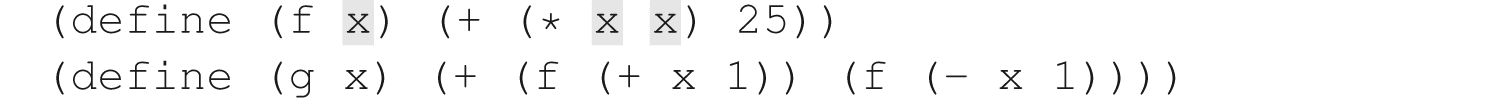
\includegraphics[width=0.85\textwidth]{images/00418.png}
\end{center}

显而易见，函数 \code{f} 中出现的 \code{x} 与函数 \code{g} 中出现的 \code{x} 完全没有任何关系。我们可以系统性地将 \code{f} 中阴影标记的 \code{x} 全部替换为 \code{y}，函数计算出的结果依然毫无二致。简而言之，阴影标记的 \code{x} 仅在 \code{f} 的定义内部拥有意义，而在其他任何地方均不存在。

同时，\code{f} 的函数头中第一次出现的 \code{x} 与其函数体内部出现的 \code{x} 性质完全不同。当我们求值 \code{(f n)} 时，函数名 \code{f} 彻底消失，而函数体内的 \code{x} 则被统一替换为实参 \code{n}。为了区分变量的这两种角色：
\begin{itemize}
  \item 我们将出现在函数头（或形参列表）中的变量称为\term{绑定出现}（binding occurrence）；
  \item 将出现在函数体内部被引用的变量称为\term{约束出现}（bound occurrence）；
  \item 我们称 \code{x} 的绑定出现\textbf{约束}了 \code{f} 体内所有出现的 \code{x}；
  \item 某个绑定出现所管辖并生效的代码区域，被称为其\term{词法作用域}（lexical scope）。
\end{itemize}

上述程序在顶层还绑定了两个名字：\code{f} 和 \code{g}。它们的作用域被称为\term{顶层作用域}（top-level scope）。

反之，若某个变量在所处环境中没有任何绑定出现，它就被称为\term{自由出现}（free occurrence，即自由变量）。自由变量是没有定义的名称——既不是语言内建的，也不是由库引入的，更没有在当前程序中定义。例如在 DrRacket 交互区中分别输入 \code{f}、\code{g} 和 \code{x}：

\begin{replbox}
> f
f
> g
g
> x
x: this variable is not defined
\end{replbox}

词法作用域可以用精巧的箭头图来具象化表示：

\begin{center}
  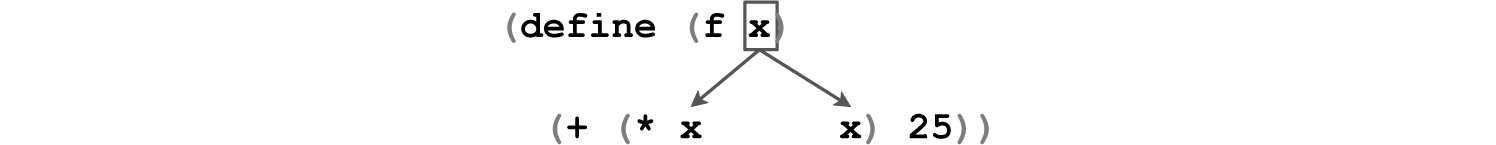
\includegraphics[width=0.85\textwidth]{images/00419.png}
\end{center}

\begin{notebox}[DrRacket 的语法检查图示]
点击 DrRacket 右上角的“Check Syntax”（检查语法）按钮，将鼠标悬停在变量上方，DrRacket 会自动绘制出完全一致的词法绑定箭头！
\end{notebox}

图~\ref{fig:00420_toplevel} 展示了顶层作用域的绑定关系：

\begin{center}
  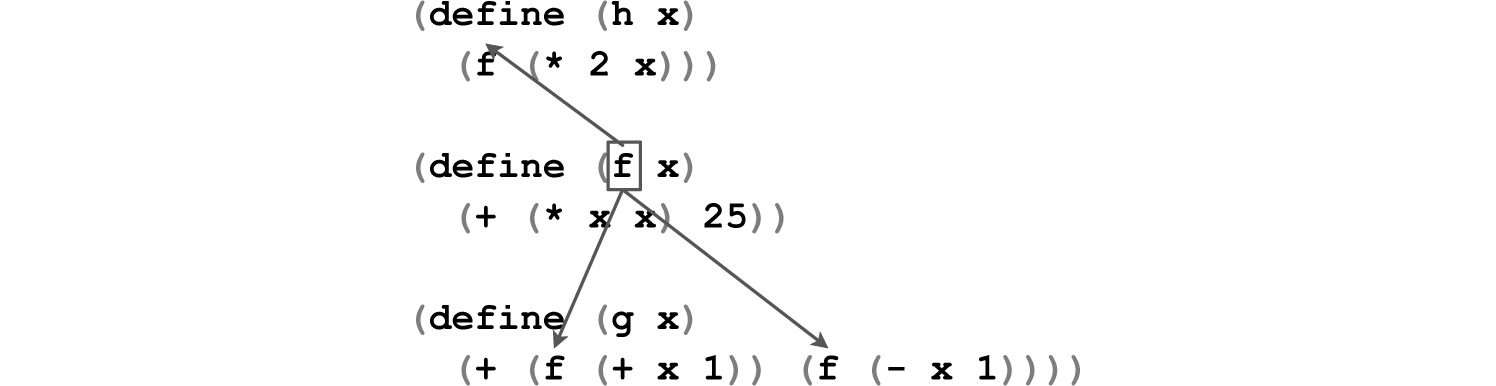
\includegraphics[width=0.85\textwidth]{images/00420.png}
  \captionof{figure}{顶层作用域绑定关系}\label{fig:00420_toplevel}
\end{center}

\code{f} 的绑定出现带有圆点标记，射出的箭头指向它所有生效的被调用处。这些图示同样精准地解释了变量重命名的本质原理：\textbf{重命名形参，就是找到其词法作用域内的所有约束出现并同步替换}。

\begin{exercise}{绘制词法绑定箭头}{300}
考虑以下简单的 ISL+ 程序：

\begin{center}
  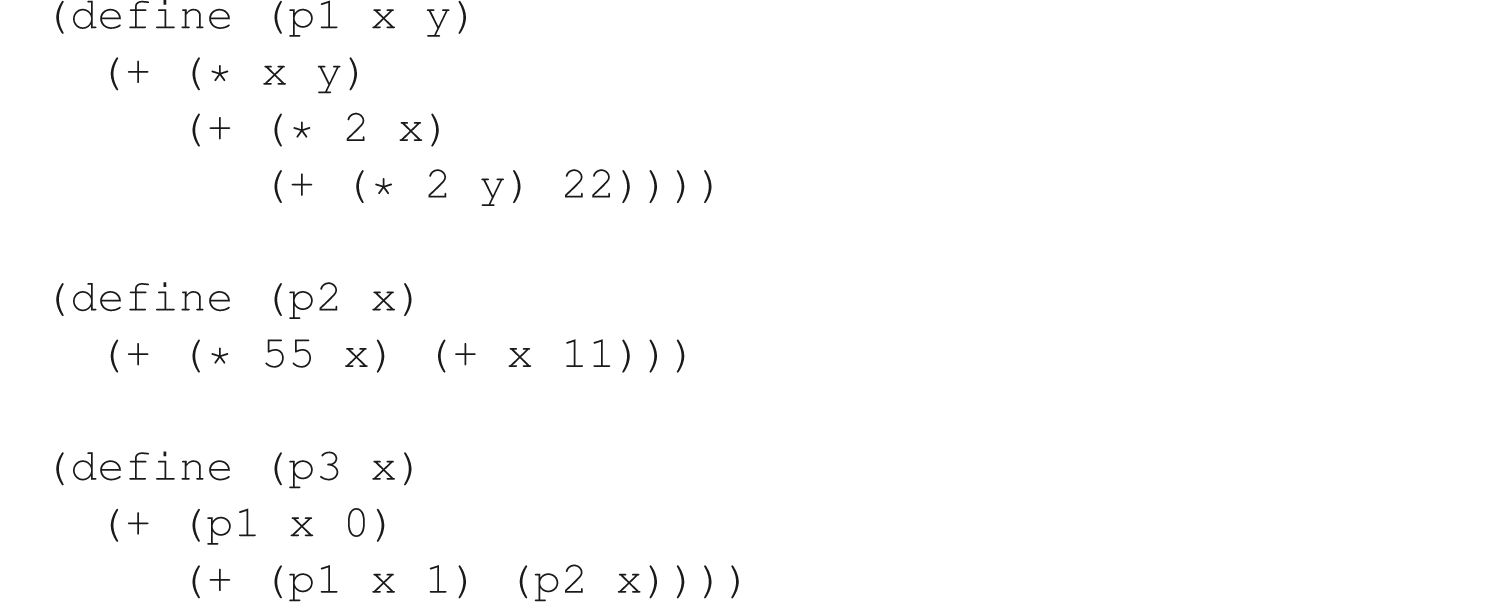
\includegraphics[width=0.85\textwidth]{images/00421.png}
\end{center}

从 \code{p1} 的参数 \code{x} 出发，绘制箭头指向其管辖的所有约束出现。再从 \code{p1} 本身出发，绘制箭头指向所有调用 \code{p1} 的位置。在 DrRacket 中使用“Check Syntax”功能验证你的答案。
\end{exercise}

与全局顶层定义不同，\code{local} 内部定义的可见范围被严格限制：\textbf{局部定义的作用域就是当前所属的整个 \code{local} 表达式}：

\begin{center}
  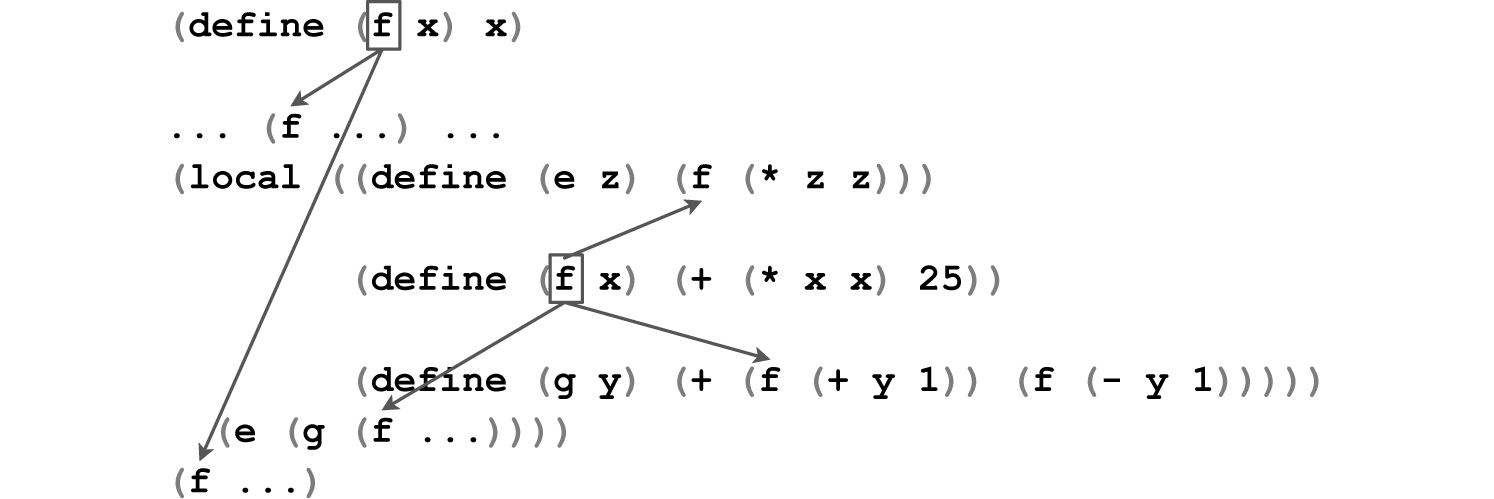
\includegraphics[width=0.85\textwidth]{images/00422.png}
\end{center}

在 \code{local} 之外出现的同名标识符完全不受局部定义的管辖。

由于作用域是一个连续的代码文本区域，计算机科学家常用\term{作用域轮廓框}（scope boxes）来直观界定范围：

\begin{center}
  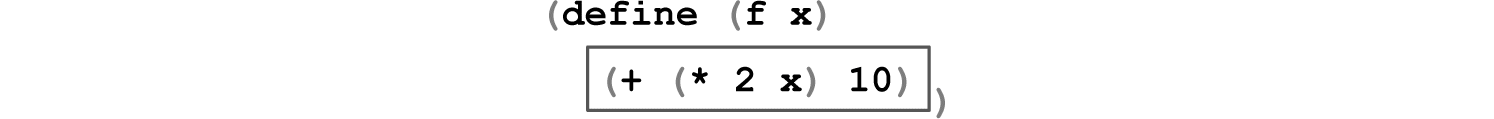
\includegraphics[width=0.85\textwidth]{images/00423.png}
\end{center}

对于 \code{local}，方框则包裹住整个 \code{local} 表达式：

\begin{center}
  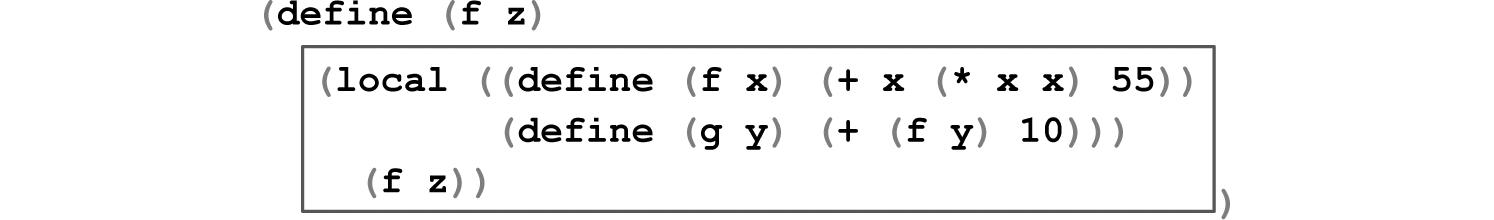
\includegraphics[width=0.85\textwidth]{images/00424.png}
\end{center}

借助方框图，我们可以轻易理解当内部局部定义重用了外层的变量名时所发生的\term{变量遮蔽}（shadowing）与\term{作用域空洞}（holes in scope）：

\begin{center}
  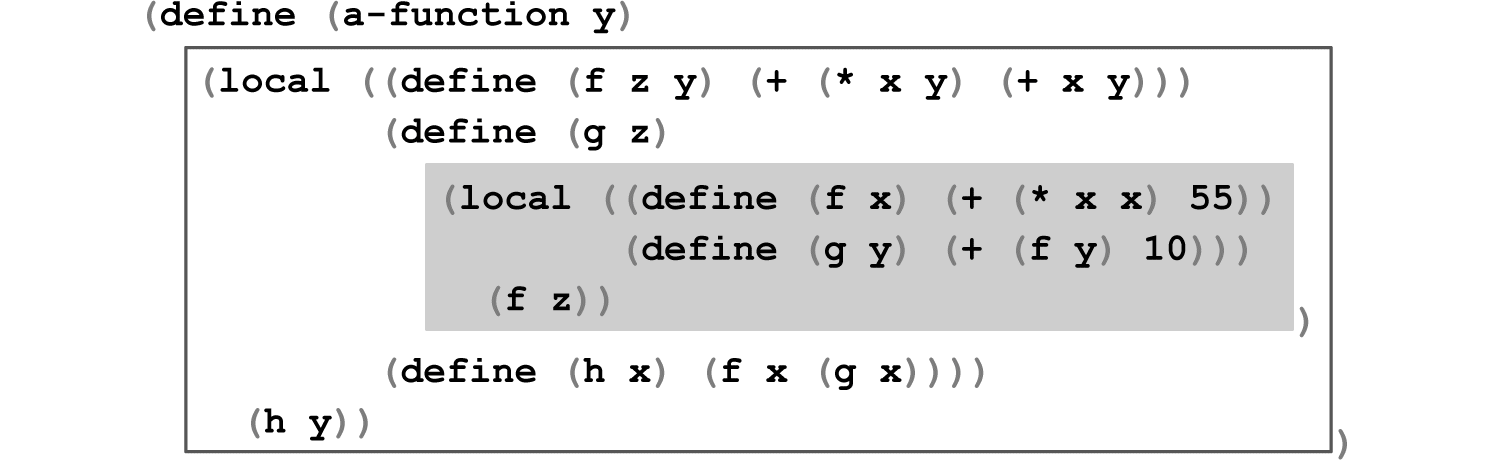
\includegraphics[width=0.85\textwidth]{images/00425.png}
\end{center}

灰色框表示内层 \code{f} 的作用域，白色框表示外层 \code{f} 的作用域。落在灰色框内部的调用一律指向内层定义；只有落在白框且在灰框之外的调用才指向外层定义。灰色框相当于在外层作用域中挖出了一个“空洞”。

在参数命名中同样可能产生空洞：

\begin{center}
  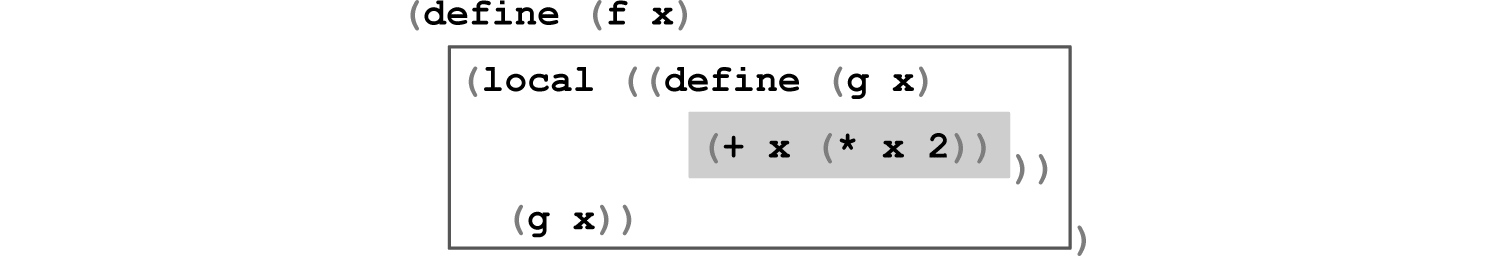
\includegraphics[width=0.85\textwidth]{images/00426.png}
\end{center}

总体而言，程序的词法作用域始终构成了一套层次分明、逐步嵌套的几何轮廓体系。

\begin{exercise}{为排序程序绘制词法作用域轮廓框}{301}
在图~\ref{fig:105} 中，为 \code{sort} 和 \code{alon} 的每个绑定出现画出作用域方框，并画出从引用指向绑定的箭头。然后在图~\ref{fig:106} 的变体上重复此练习。除了变量名称不同之外，这两个函数的行为有何区别？

\begin{center}
  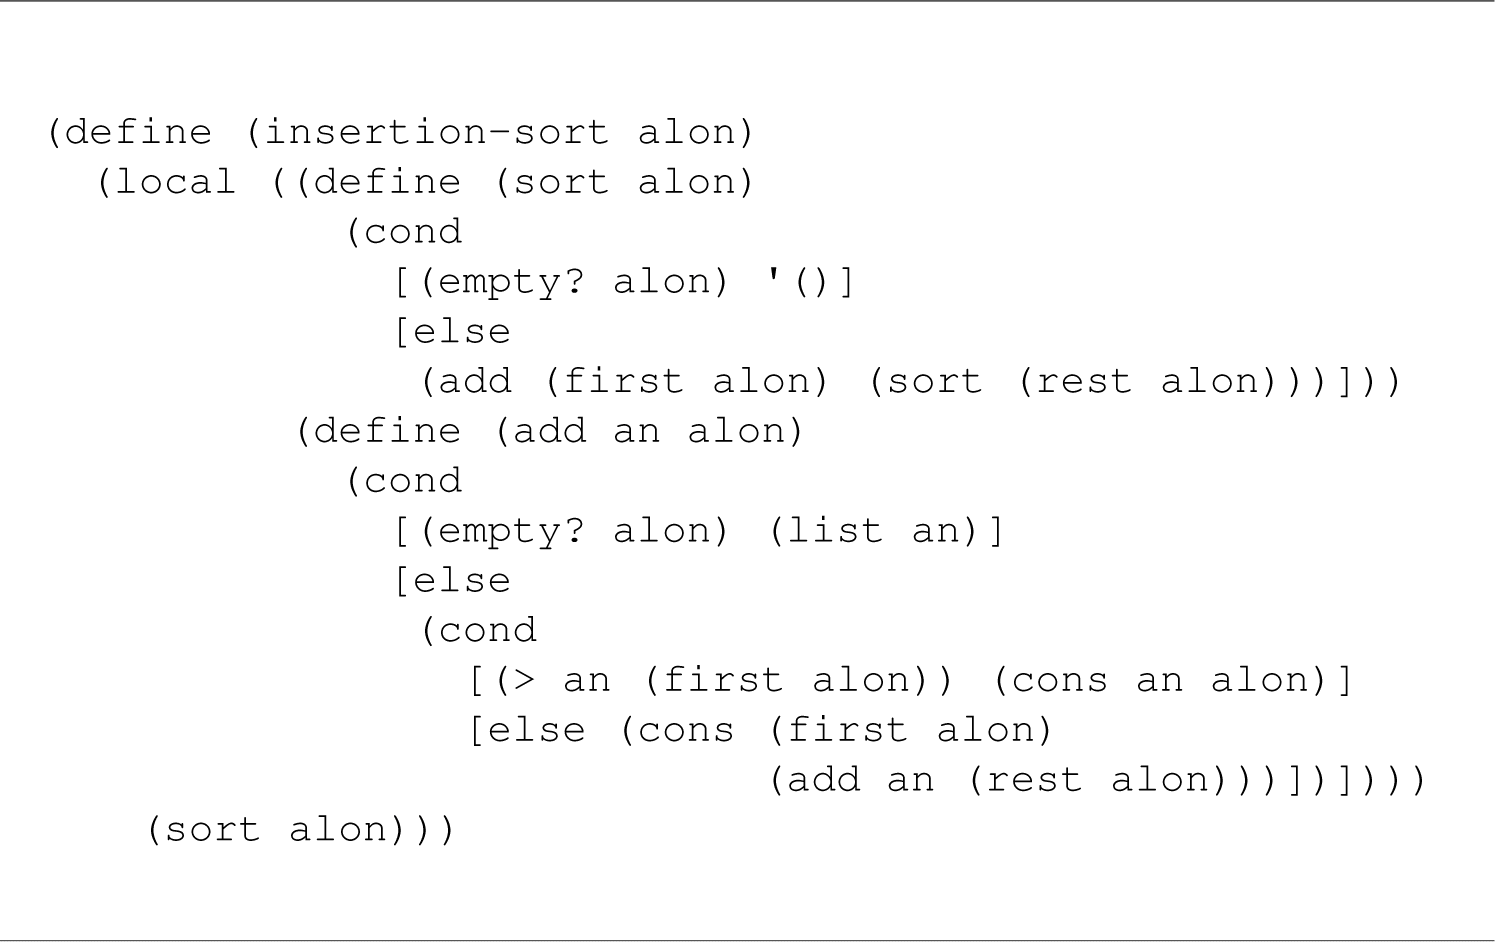
\includegraphics[width=0.85\textwidth]{images/00427.png}
  \captionof{figure}{练习 301 的词法作用域轮廓 (版本 1)}\label{fig:105}
\end{center}

\begin{center}
  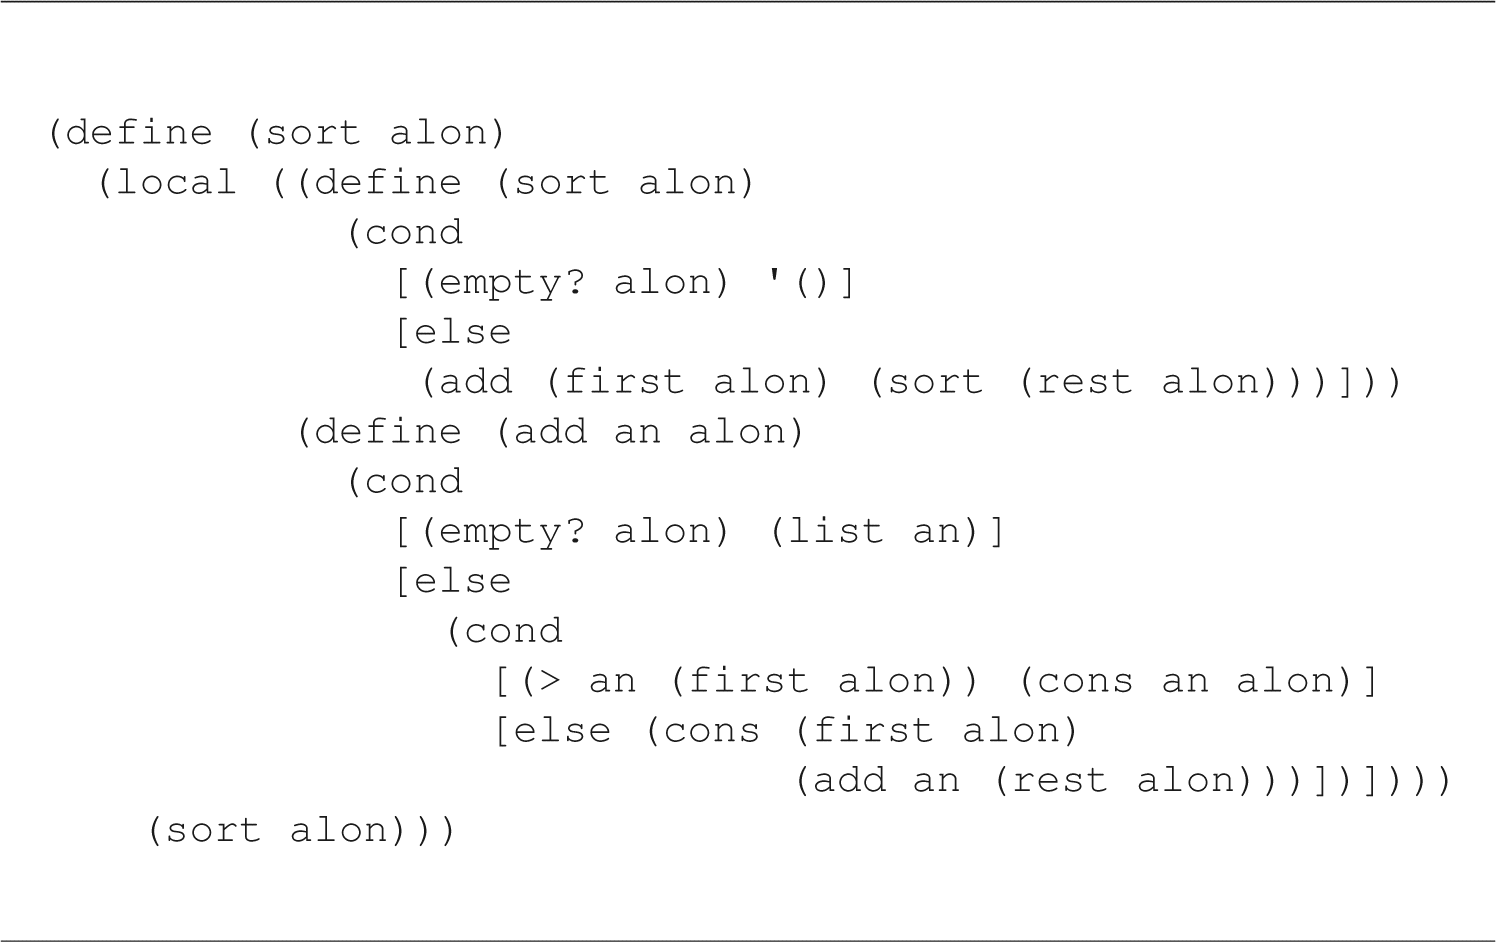
\includegraphics[width=0.85\textwidth]{images/00428.png}
  \captionof{figure}{练习 301 的词法作用域轮廓 (版本 2)}\label{fig:106}
\end{center}
\end{exercise}

\begin{exercise}{常量的自引用陷阱}{302}
回顾每个变量的值均来自于其绑定出现。考虑以下定义：
\begin{lstlisting}[language=BSL]
(define x (cons 1 x))
\end{lstlisting}
右侧阴影中的 \code{x} 在哪里被绑定？既然这是一个普通常量定义而非函数定义，右侧表达式必须被立刻求值。根据求值法则，右侧表达式的值应当是什么？在 DrRacket 中运行会发生什么？
\end{exercise}

对于 \code{lambda} 表达式，其形参的作用域就是其整个函数体表达式：

\begin{center}
  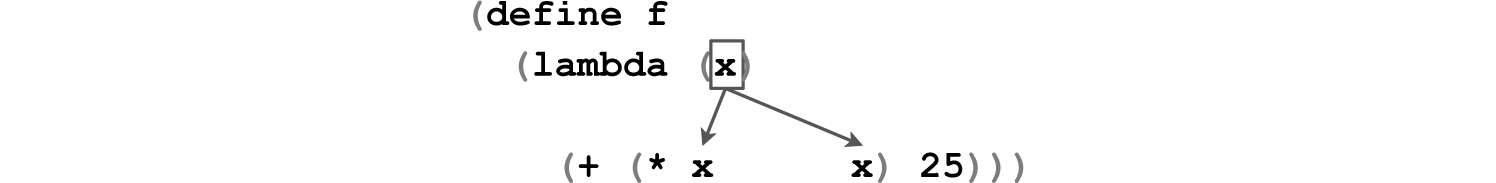
\includegraphics[width=0.85\textwidth]{images/00429.png}
\end{center}

\begin{exercise}{lambda 表达式中的绑定分析}{303}
在以下三个 \code{lambda} 表达式中，分别从阴影标记的 \code{x} 出发，绘制箭头指向其真正的绑定出现：

\begin{center}
  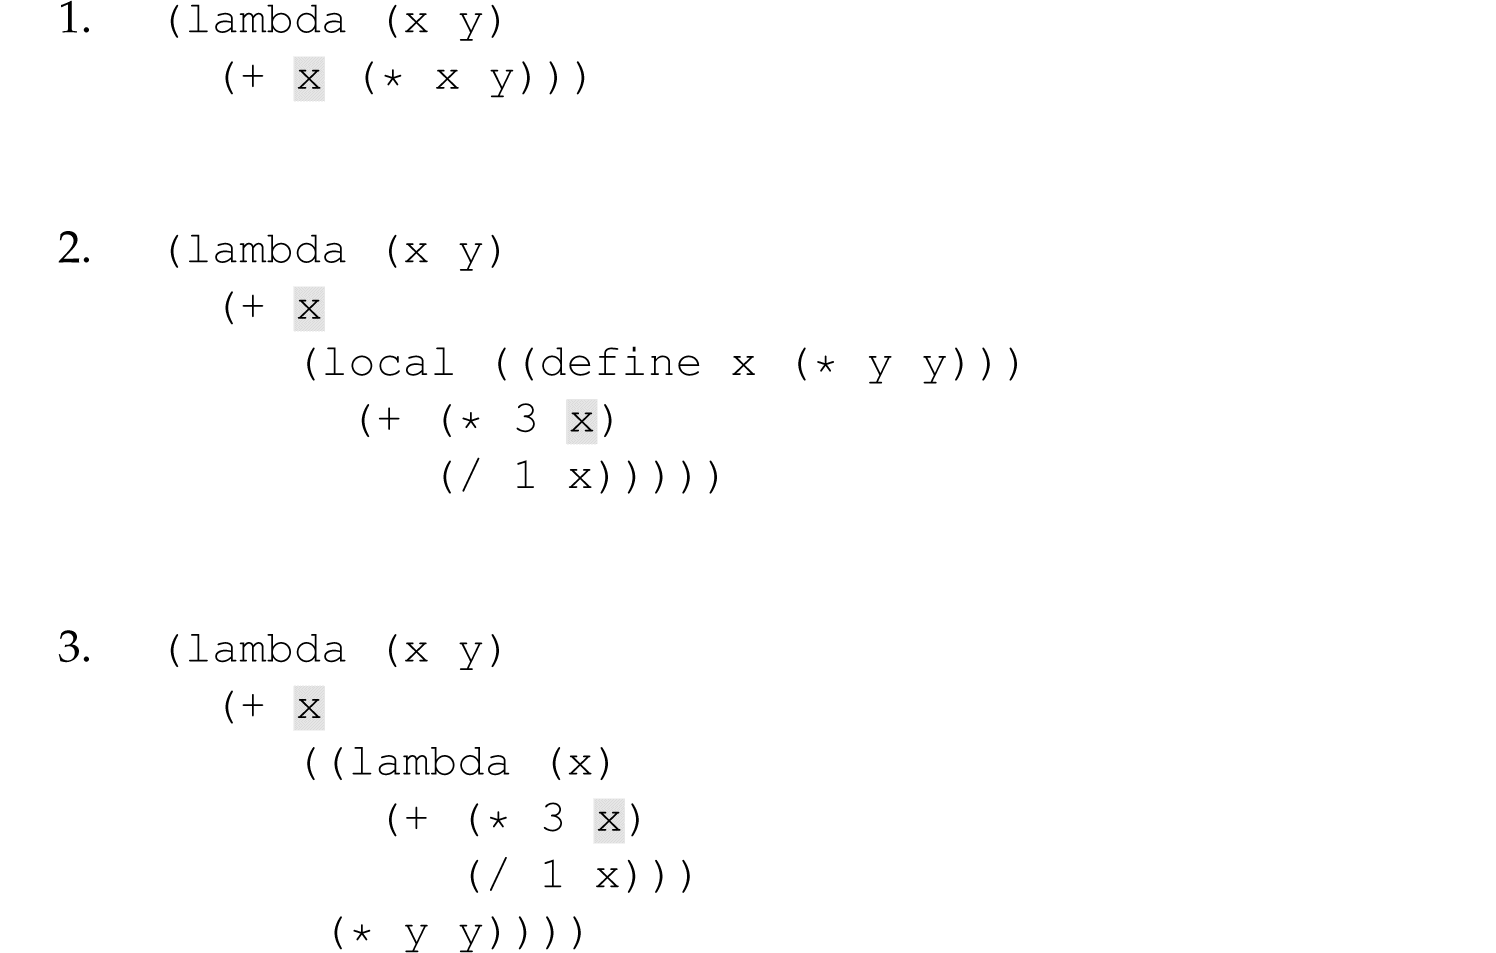
\includegraphics[width=0.85\textwidth]{images/00430.png}
\end{center}

并为每个作用域绘制方框及必要的空洞。
\end{exercise}

% ------------------------------------------------------------------------------
\intermezzosection{ISL 的 for 推导式 (ISL for Loops)}
\label{sec:intermezzo03_loops}

虽然第三部分从未直接使用“循环”这个词，但我们一直在进行循环操作。从本质上说，\term{循环}（loop）就是遍历复合数据并逐一处理其元素，同时合成新的数据结构。例如，\code{map} 遍历列表并收集变换结果；\code{build-list} 遍历自然数区间并构造成新列表。

\begin{notebox}[加载抽象拓展库]
要使用本节介绍的高级循环与模式匹配，请在定义区顶部添加：
\begin{lstlisting}[language=BSL]
(require 2htdp/abstraction)
\end{lstlisting}
\end{notebox}

ISL+ 中的循环与传统命令式语言有着根本不同：传统循环往往通过副作用修改内存，而不直接产出新的复合数据；而 ISL+ 的循环专注于\textbf{纯函数式的数据变换与聚合}。此外，语法形式的循环相比纯函数组合具有两大优势：首先，其语法结构能更加醒目地表达编程意图；其次，编译器通常能将语法循环优化为速度更快的底层机器指令。

图~\ref{fig:107} 给出了扩展的 for 推导式文法：

\begin{center}
  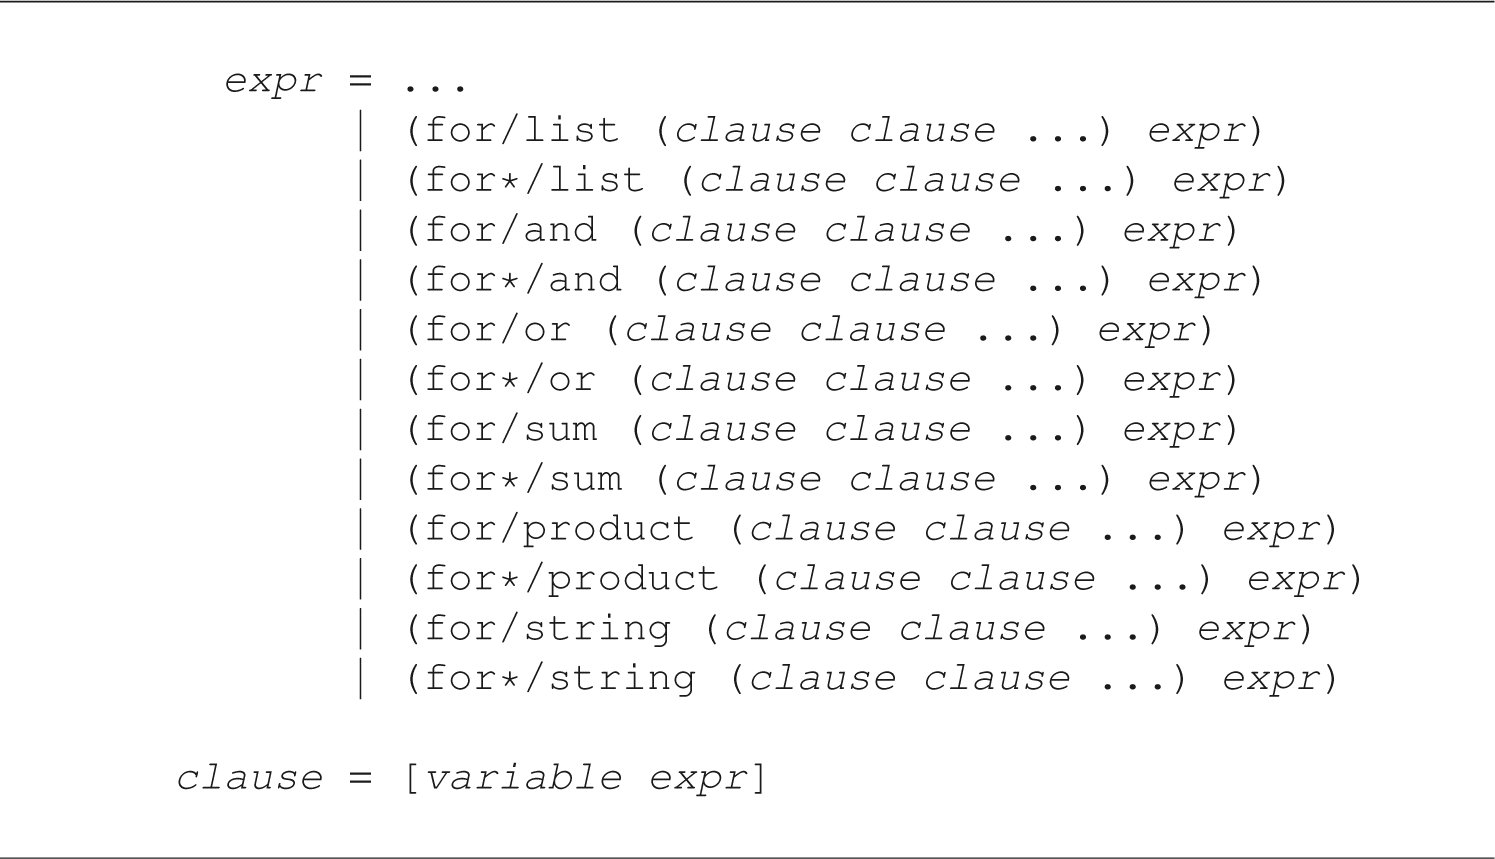
\includegraphics[width=0.85\textwidth]{images/00431.png}
  \captionof{figure}{ISL+ 拓展的 for 推导式文法}\label{fig:107}
\end{center}

文法清晰地呈现出成对出现的六组循环构造：\code{for} 与 \code{for*}，分别对应于 \code{list}、\code{and}、\code{or}、\code{sum}、\code{product} 和 \code{string}。

两者的核心区别在于\textbf{词法作用域与遍历维度}：
\begin{itemize}
  \item \code{for} 形式是\textbf{并行遍历}（parallel traversal），各子句中的序列同时前进一步，且后续子句\textbf{不能}引用前面子句引入的循环变量；
  \item \code{for*} 形式是\textbf{嵌套笛卡尔积遍历}（nested traversal），类似多重嵌套循环，且后续子句\textbf{可以}自由引用前面子句绑定的循环变量！
\end{itemize}

\begin{center}
  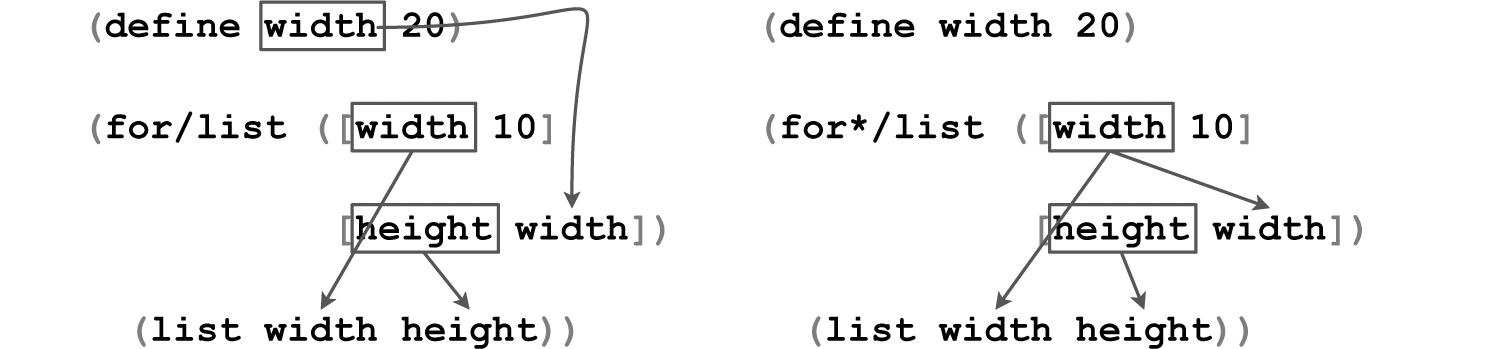
\includegraphics[width=0.85\textwidth]{images/00432.png}
\end{center}

\code{for/list} 的语义极其简洁自然：
\begin{replbox}
> (for/list ([i 10]) i)
(list 0 1 2 3 4 5 6 7 8 9)
\end{replbox}
这直接等价于 \code{(build-list 10 (lambda (i) i))}！

两个序列的并行拉链组合（zip）：
\begin{center}
  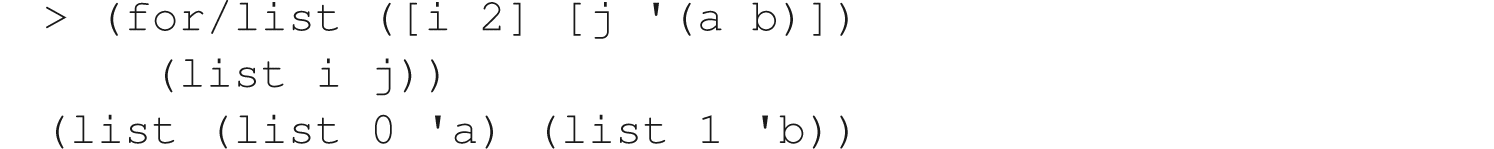
\includegraphics[width=0.85\textwidth]{images/00433.png}
\end{center}
对比纯函数式的写法（图~\ref{fig:00434_zip_plain}），\code{for/list} 展现出了惊人的可读性：
\begin{center}
  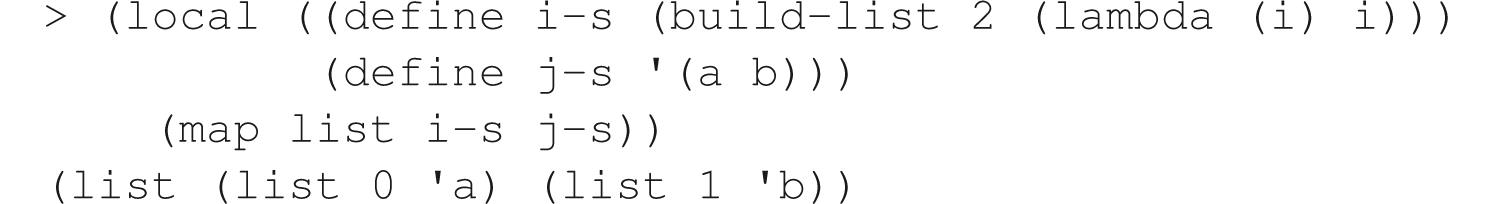
\includegraphics[width=0.85\textwidth]{images/00434.png}
  \captionof{figure}{列表组合处理代数形式}\label{fig:00434_zip_plain}
\end{center}

\begin{notebox}[样例问题：设计 enumerate 函数]
设计函数 \code{enumerate}，接收一个列表，产生由每个元素与其对应的索引编号组成的二元对列表。
\end{notebox}

借助 \code{for/list}，解法极其优雅自然：
\begin{lstlisting}[language=BSL]
; [List-of X] -> [List-of [List N X]]
(check-expect (enumerate '(a b c)) '((1 a) (2 b) (3 c)))
(define (enumerate lx)
  (for/list ([x lx] [ith (length lx)])
    (list (+ ith 1) x)))
\end{lstlisting}

相比之下，\code{for*/list} 则展开为嵌套循环（笛卡尔积）：

\begin{center}
  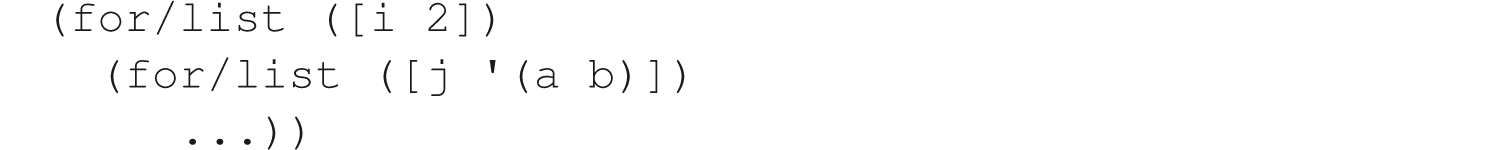
\includegraphics[width=0.85\textwidth]{images/00435.png}
\end{center}

\begin{exercise}{对比 for/list 与 for*/list}{304}
在 DrRacket 交互区中分别求值：
\begin{lstlisting}[language=BSL]
(for/list ([i 2] [j '(a b)]) (list i j))
(for*/list ([i 2] [j '(a b)]) (list i j))
\end{lstlisting}
对比两者的输出结构差异。
\end{exercise}

图~\ref{fig:00436_interaction}、\ref{fig:00437_table} 和 \ref{fig:00438_nest} 详细演示了两者在多子句依赖下的行为细节：

\begin{center}
  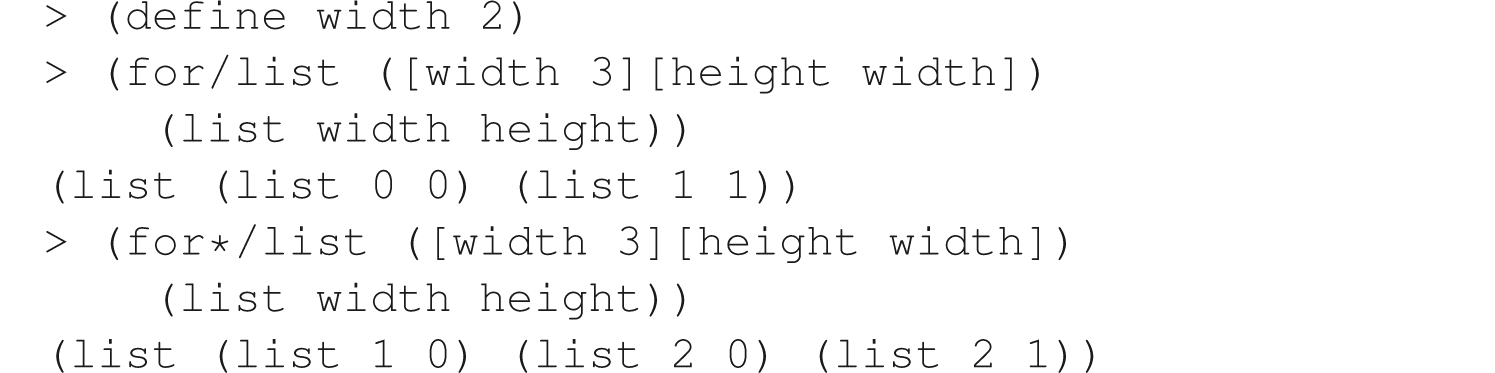
\includegraphics[width=0.85\textwidth]{images/00436.png}
  \captionof{figure}{语法结构交互分析}\label{fig:00436_interaction}
\end{center}

\begin{center}
  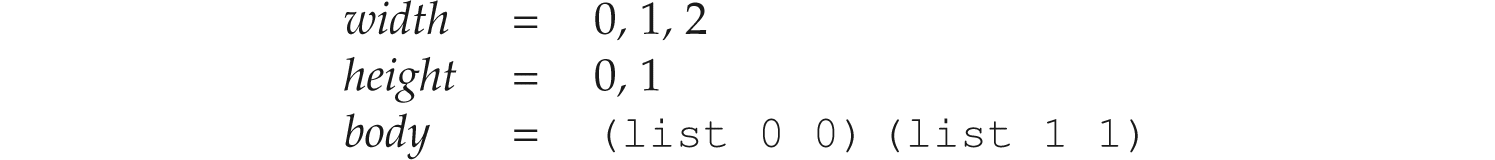
\includegraphics[width=0.85\textwidth]{images/00437.png}
  \captionof{figure}{语法结构对照表}\label{fig:00437_table}
\end{center}

\begin{center}
  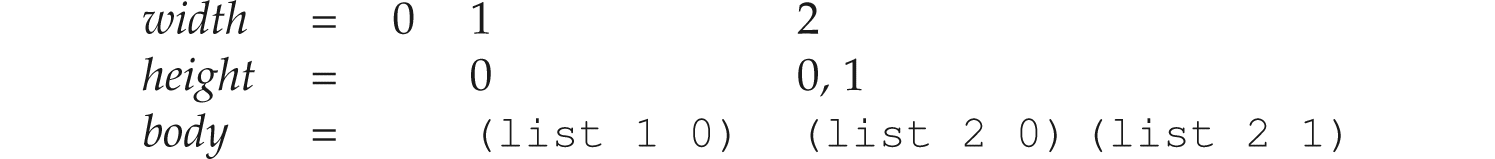
\includegraphics[width=0.85\textwidth]{images/00438.png}
  \captionof{figure}{嵌套语法分析}\label{fig:00438_nest}
\end{center}

借助 \code{for*/list}，计算两个列表的笛卡尔乘积函数 \code{cross} 可以轻松写出：

\begin{center}
  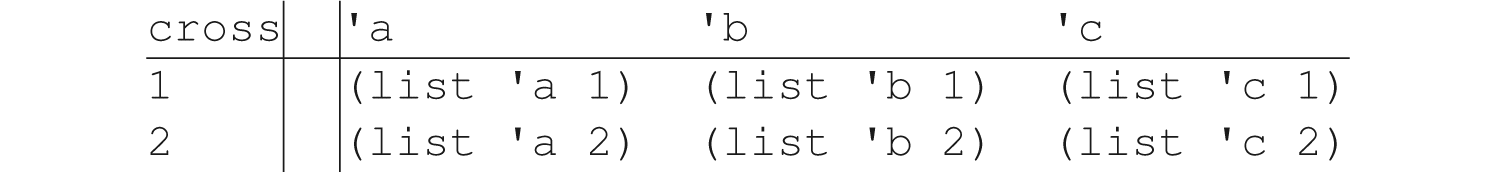
\includegraphics[width=0.85\textwidth]{images/00439.png}
\end{center}

\begin{center}
  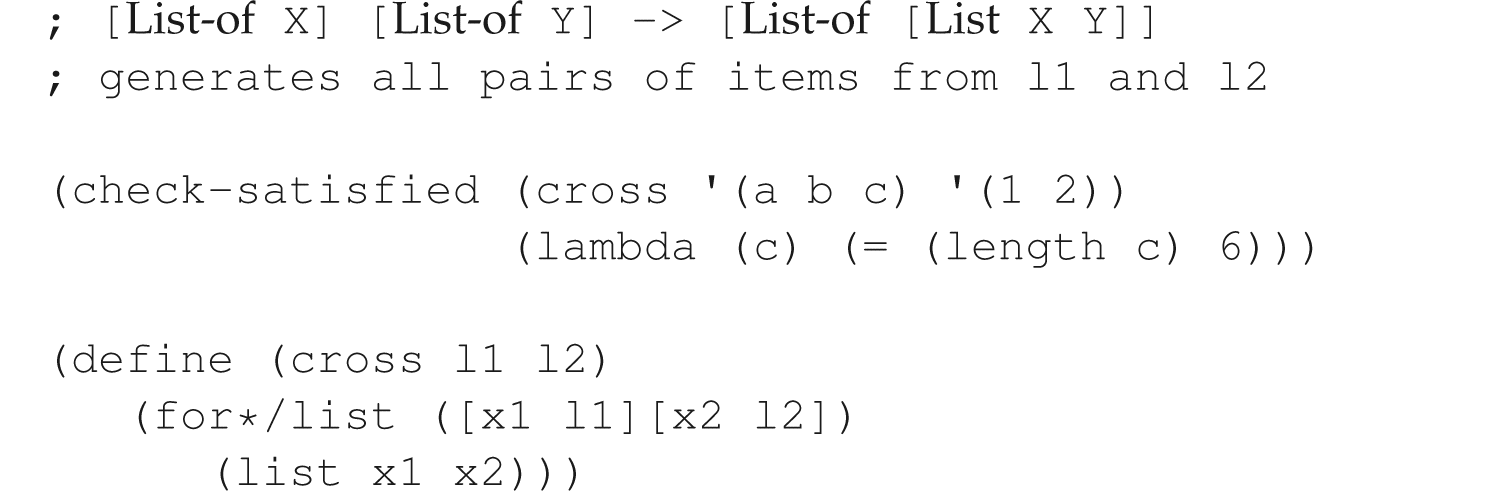
\includegraphics[width=0.85\textwidth]{images/00440.png}
\end{center}

图~\ref{fig:108} 更是展现了抽象的无上威力：仅用 5 行代码，通过 \code{for*/list} 搞定了第 12.4 节极为复杂的字母全排列生成算法！

\begin{center}
  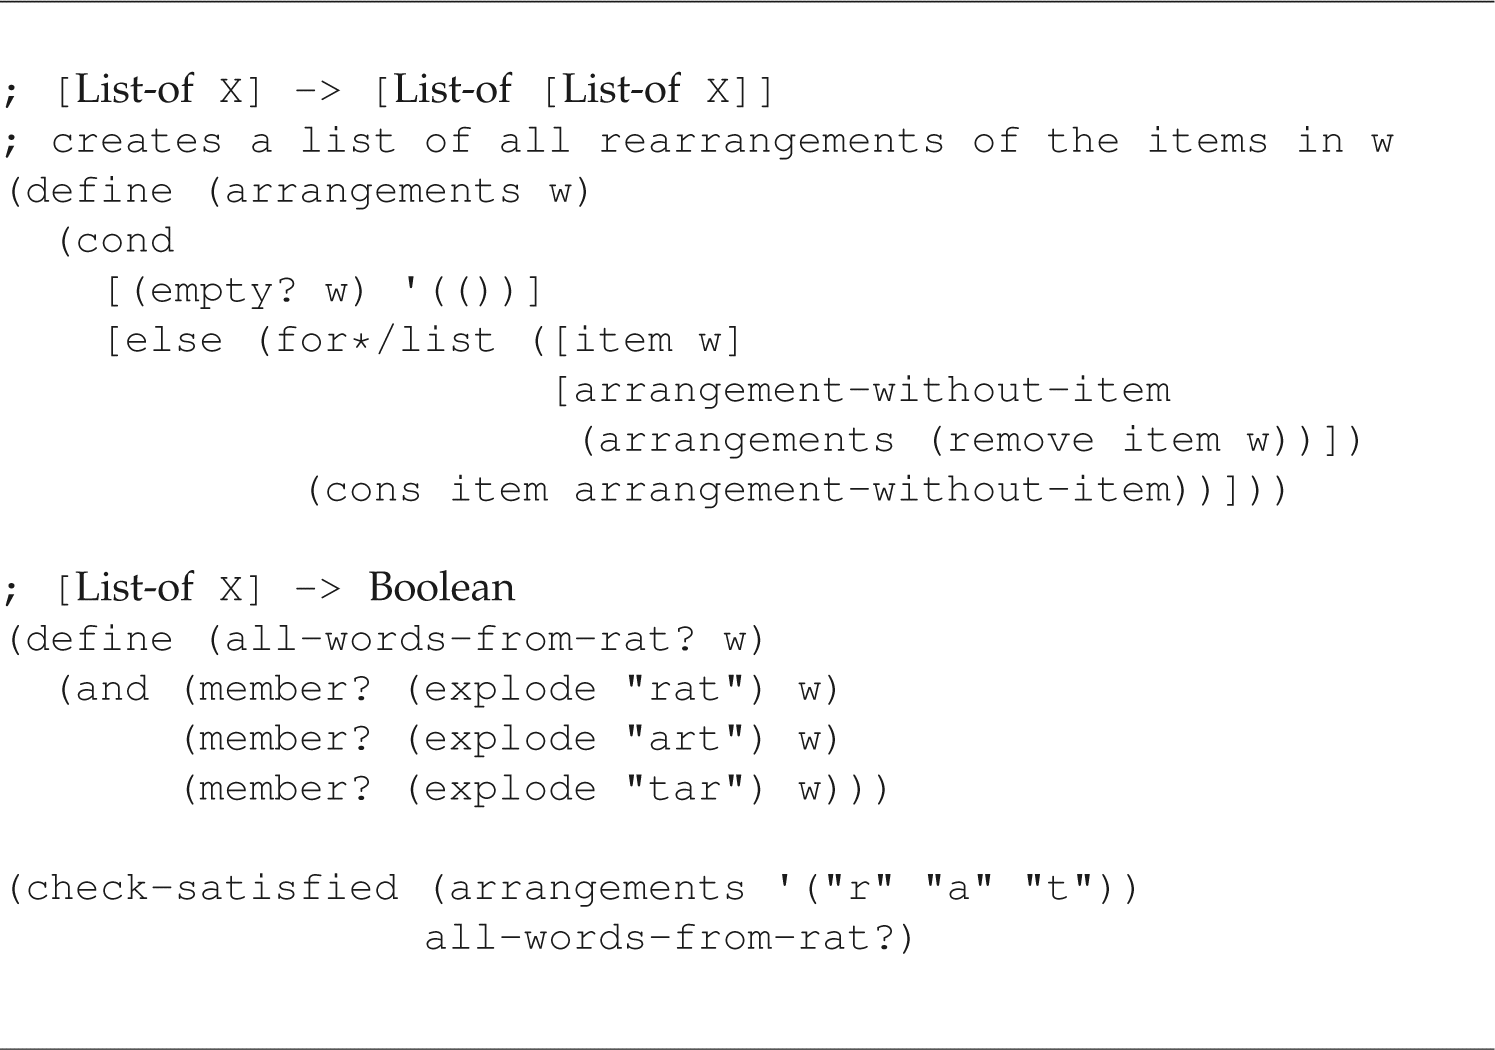
\includegraphics[width=0.85\textwidth]{images/00441.png}
  \captionof{figure}{利用 for*/list 紧凑实现的字母全排列程序}\label{fig:108}
\end{center}

其他循环变体同样顾名思义：
\begin{itemize}
  \item \code{for/and}：用 \code{and} 汇聚所有迭代结果；
  \item \code{for/or}：用 \code{or} 汇聚，返回首个非假值；
  \item \code{for/sum}：将每次迭代计算出的数值求和；
  \item \code{for/product}：将每次迭代的值累乘；
  \item \code{for/string}：将单字符拼接为新字符串。
\end{itemize}

配合图~\ref{fig:109} 中的无限自然数发生器 \code{in-naturals} 和步长发生器 \code{in-range}，循环的能力进一步大放异彩：

\begin{center}
  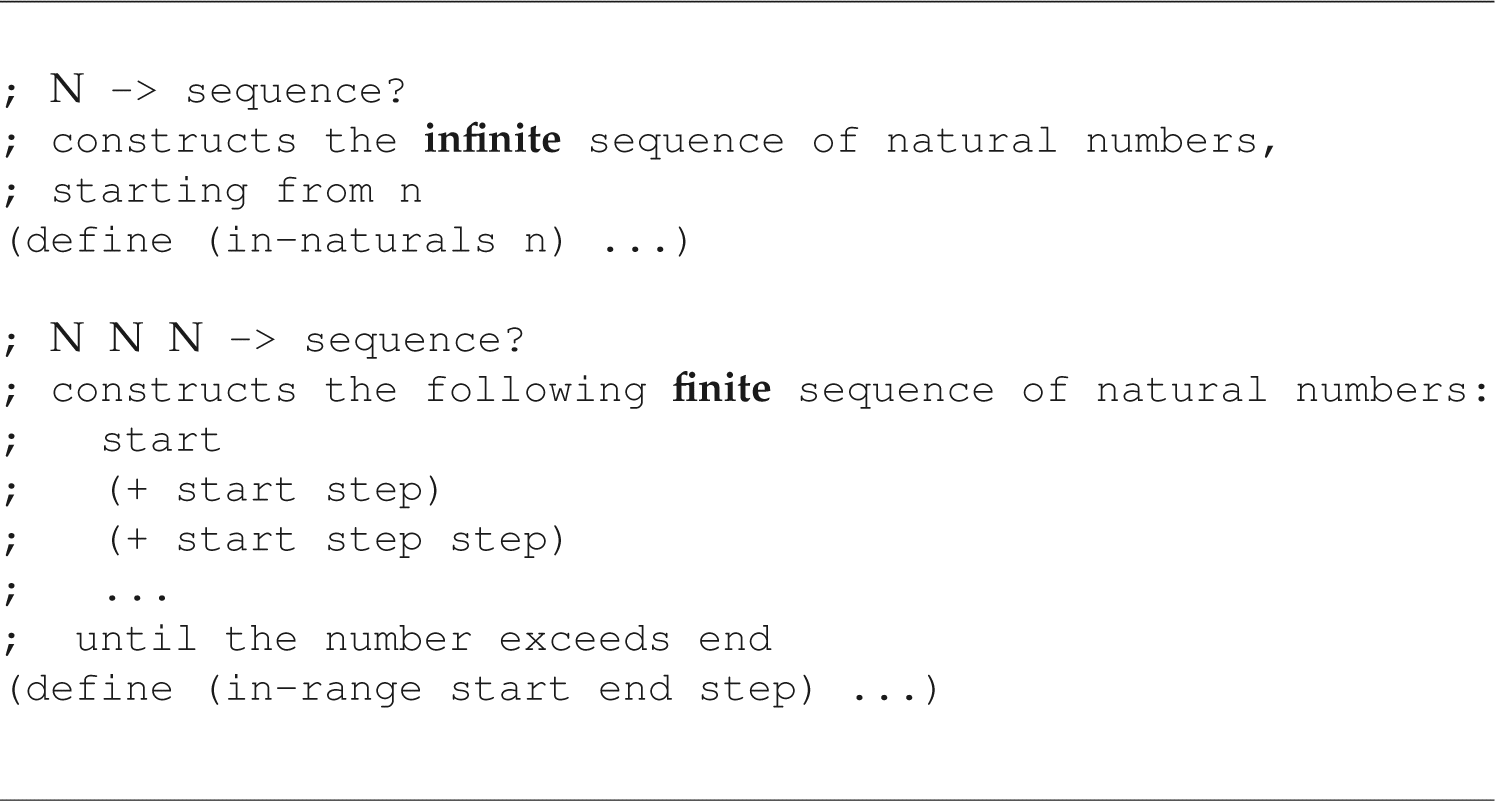
\includegraphics[width=0.85\textwidth]{images/00442.png}
  \captionof{figure}{构造自然数序列的高级生成器}\label{fig:109}
\end{center}

例如简洁定义求前 $n$ 个偶数和的函数：
\begin{lstlisting}[language=BSL]
; N -> Number
(define (sum-evens n)
  (for/sum ([i (in-range 0 n 2)]) i))
\end{lstlisting}

\begin{exercise}{使用循环重构 convert-euro}{305}
使用 \code{for/list} 重新实现练习 267 中的货币转换函数 \code{convert-euro}。
\end{exercise}

\begin{exercise}{使用循环生成各类列表}{306}
使用 \code{for/list} 分别实现：
\begin{enumerate}
  \item 生成列表 \code{(list 0 ... (- n 1))}；
  \item 生成列表 \code{(list 1 ... n)}；
  \item 生成列表 \code{(list 1 1/2 ... 1/n)}；
  \item 生成前 $n$ 个偶数列表；
  \item 重新实现练习 262 中的单位对角方阵 \code{identityM}。
\end{enumerate}
最后，使用 \code{for/list} 重新实现练习 250 中的制表函数 \code{tabulate}。
\end{exercise}

\begin{exercise}{使用 for/or 查找名字}{307}
使用 \code{for/or} 定义 \code{find-name}，检索列表中首个匹配前缀的名字。并定义一个函数，确保列表中没有名字的长度超过给定宽度。
\end{exercise}

% ------------------------------------------------------------------------------
\intermezzosection{模式匹配 (Pattern Matching)}
\label{sec:intermezzo03_match}

当我们为具有多个分支的数据定义设计函数时，传统做法是使用多分支的 \code{cond} 表达式：在每个分支中用类型谓词进行判定，若匹配成功，再使用大量的\textbf{选择器}（selectors）层层拆解复合数据。前三部分反复练习了这一流程。

然而，重复的代码模式呼唤着语言级的抽象！函数式编程语言的设计者们引入了\term{模式匹配}（Pattern Matching，在 ISL+ 中表现为 \code{match} 表达式），将类型判定谓词与字段提取选择器完美融为一体。

图~\ref{fig:110} 给出了 \code{match} 的文法规范：

\begin{center}
  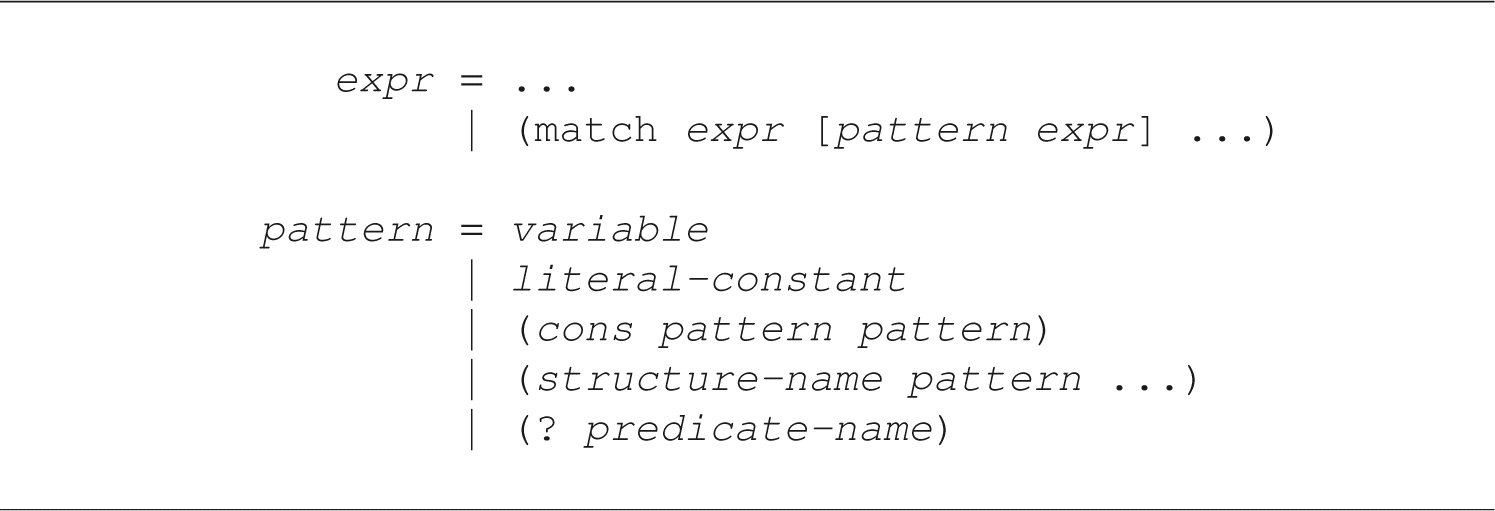
\includegraphics[width=0.85\textwidth]{images/00443.png}
  \captionof{figure}{ISL+ 模式匹配表达式文法}\label{fig:110}
\end{center}

\begin{lstlisting}[language=BSL]
(match expr
  [pattern1 expr1]
  [pattern2 expr2]
  ...)
\end{lstlisting}

与 \code{cond} 最根本的区别在于：\textbf{\code{match} 的每个模式分支都会开辟一个独立的词法作用域}！模式中出现的变量会自动绑定到被解构数据对应的组成字段上，并在该分支的表达式内部生效：

\begin{center}
  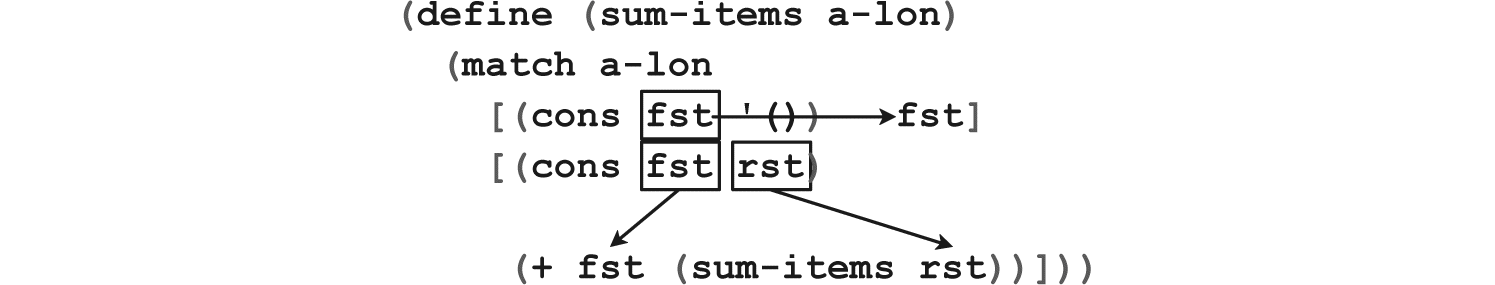
\includegraphics[width=0.85\textwidth]{images/00444.png}
\end{center}

模式匹配支持极其丰富的解构语法：
\begin{itemize}
  \item \textbf{字面量常量}：仅匹配相等的具体常量；
\begin{center}
  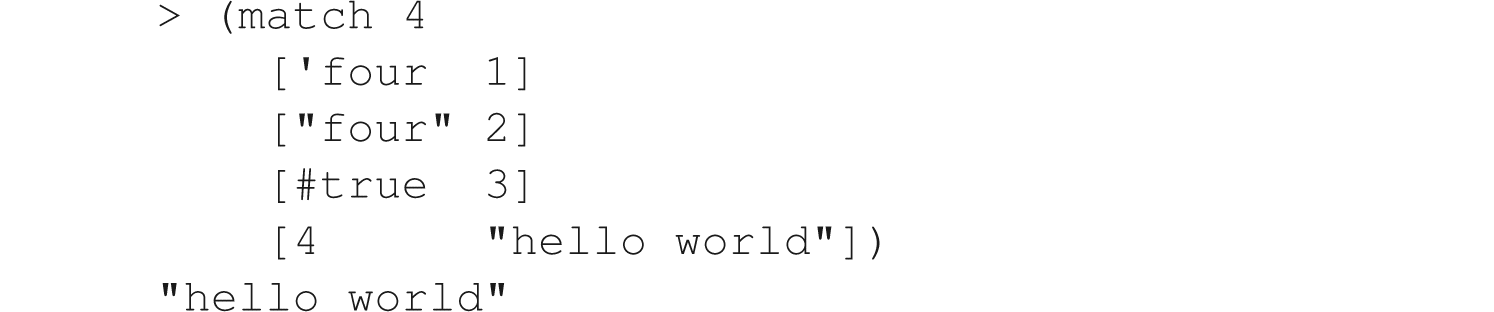
\includegraphics[width=0.85\textwidth]{images/00445.png}
\end{center}
  \item \textbf{变量模式}：匹配任意值，并将其绑定到该变量名上；
\begin{center}
  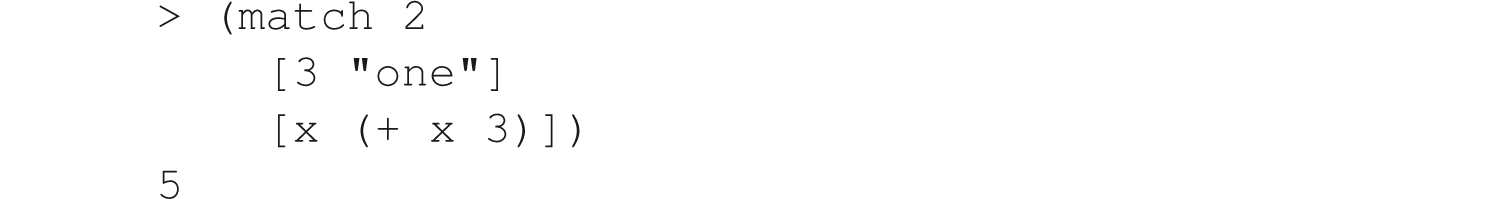
\includegraphics[width=0.85\textwidth]{images/00446.png}
\end{center}
  \item \textbf{\code{(cons p1 p2)} 列表模式}：直接解构列表的首项与剩余部分；
\begin{center}
  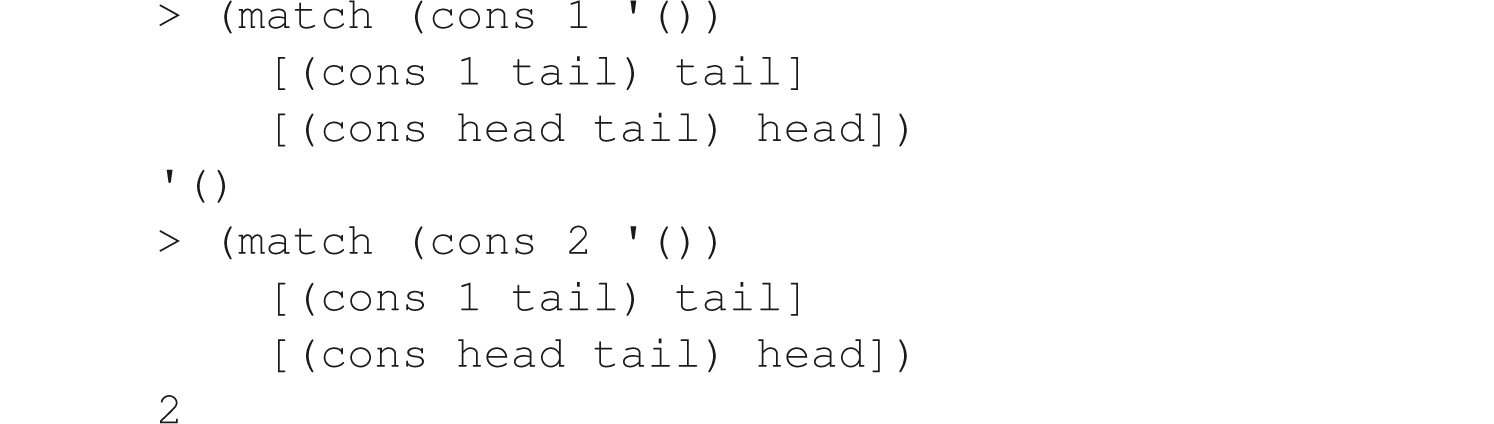
\includegraphics[width=0.85\textwidth]{images/00447.png}
\end{center}
  \item \textbf{结构体模式 \code{(struct-name p1 ... pn)}}：直接解构结构体的各个字段：
\begin{lstlisting}[language=BSL]
(define p (make-posn 3 4))
(match p
  [(posn x y) (sqrt (+ (sqr x) (sqr y)))]) ; 结果为 5
\end{lstlisting}
  \item \textbf{多层深度嵌套模式}：单次匹配即可穿透多层复合结构：
\begin{lstlisting}[language=BSL]
(match (cons (make-phone 713 664 9993) '())
  [(cons (phone area-code 664 9993) tail)
   area-code]) ; 直接提取出 713
\end{lstlisting}
  \item \textbf{谓词模式 \code{(? pred)}}：当且仅当 \code{(pred v)} 为真时匹配。
\end{itemize}

让我们通过真实问题领略 \code{match} 的非凡魅力：

\begin{notebox}[样例 1：获取非空列表的末尾元素]
\begin{lstlisting}[language=BSL]
; [Non-empty-list X] -> X
; 获取非空列表 ne-l 的最后一个元素
(check-expect (last-item '(a b c)) 'c)
(define (last-item ne-l)
  (match ne-l
    [(cons lst '()) lst]
    [(cons fst rst) (last-item rst)]))
\end{lstlisting}
\end{notebox}
无需调用任何 \code{empty?}、\code{cons?}、\code{first}、\code{rest}，模式直接镜像了数据定义本身！

\begin{notebox}[样例 2：俄罗斯套娃层数计算]
\begin{lstlisting}[language=BSL]
; RD.v2 -> N
(define (depth a-doll)
  (match a-doll
    ["doll" 0]
    [(layer c inside) (+ (depth inside) 1)]))
\end{lstlisting}
\end{notebox}

图~\ref{fig:00448_moveright} 展示了太空战游戏中向右平移目标坐标的完整实现：

\begin{center}
  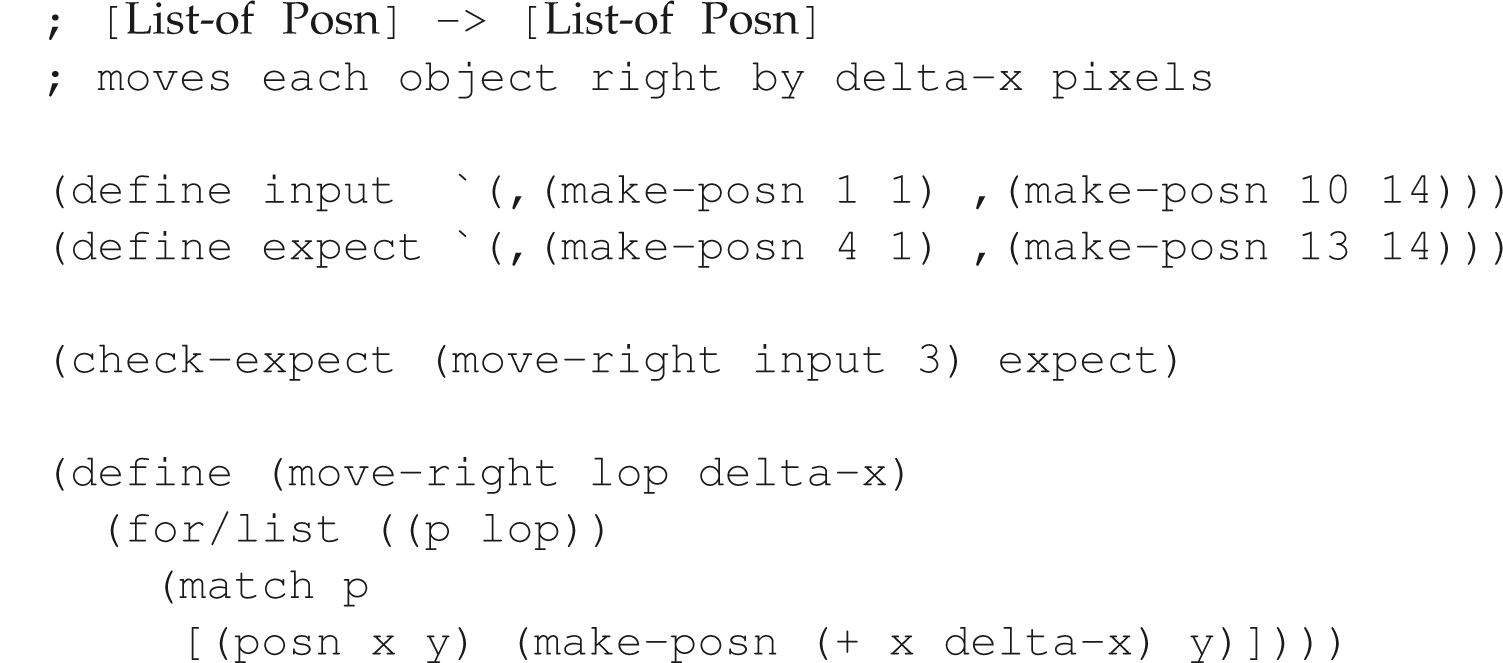
\includegraphics[width=0.85\textwidth]{images/00448.png}
  \captionof{figure}{太空战舰游戏向右移动实现}\label{fig:00448_moveright}
\end{center}

\begin{exercise}{更新电话号码区号}{308}
使用 \code{match} 设计函数 \code{replace}，将电话记录列表中所有区号为 713 的号码替换为 281。
\end{exercise}

\begin{exercise}{统计嵌套行中的词数}{309}
使用 \code{match} 设计函数 \code{words-on-line}，计算由字符串列表构成的列表中每行的单词数量。
\end{exercise}


% ==================== 第四部分：交织数据 ====================
\part{交织数据 (Intertwined Data)}
% ==============================================================================
% 第 18 章：更丰富的数据形态（树） (Chapter 18: More on Forms of Data (Trees))
% ==============================================================================

\chapter{S-表达式之美与树结构}
\label{sec:ch18_trees}

编程与诗歌有几分相似。正如诗人那样，程序员常常在看似没有现实功用的纯粹构想上磨砺技艺。他们如同上一章所解释的那样，一直在不断地修改与推敲代码。本章将引入日益复杂的数据形态——它们乍看之下似乎脱离了现实世界的具体功用。即使我们为之提供了某种启发性的背景，所选定的数据类别也纯粹到了极致，你在日后的实际开发中或许很难直接原样遇到它们。

然而，本章充分展现了设计配方的全部威力，并向你展示了现实世界程序所必须应对的复杂数据类型。为了将这些内容与你未来作为程序员的职业生涯联系起来，我们为各个小节冠以贴切的名称：树（trees）、森林（forests）与 S-表达式（S-expressions）。这些概念构成了现实世界处理诸如层次结构、文件系统乃至 XML 等复杂数据的理论基石。

\section{树 }
\label{sec:19.1_trees}

我们每个人都有一张家谱（family tree）。绘制家谱的一种直观方式是：每当一个孩子出生时，就添加一个元素，并将其连接到其父亲与母亲的元素上。对于那些父母未知的人，则无需引出连线。这种记录方式被称为\term{祖先家谱}（ancestor family tree），因为对于任意给定的人，树上的指针都指向上溯的所有已知祖先。

图~\ref{fig:111} 展示了一个三代的家谱。Gustav 是 Eva 与 Fred 的孩子，而 Eva 又是 Carl 与 Bettina 的孩子。除人名与亲属关系外，该树还记录了出生年份与眼睛颜色。基于这幅草图，你很容易想象一个延伸多代的庞大家谱，或者记录更多维信息的家谱。

\begin{figure}[htbp]
  \centering
  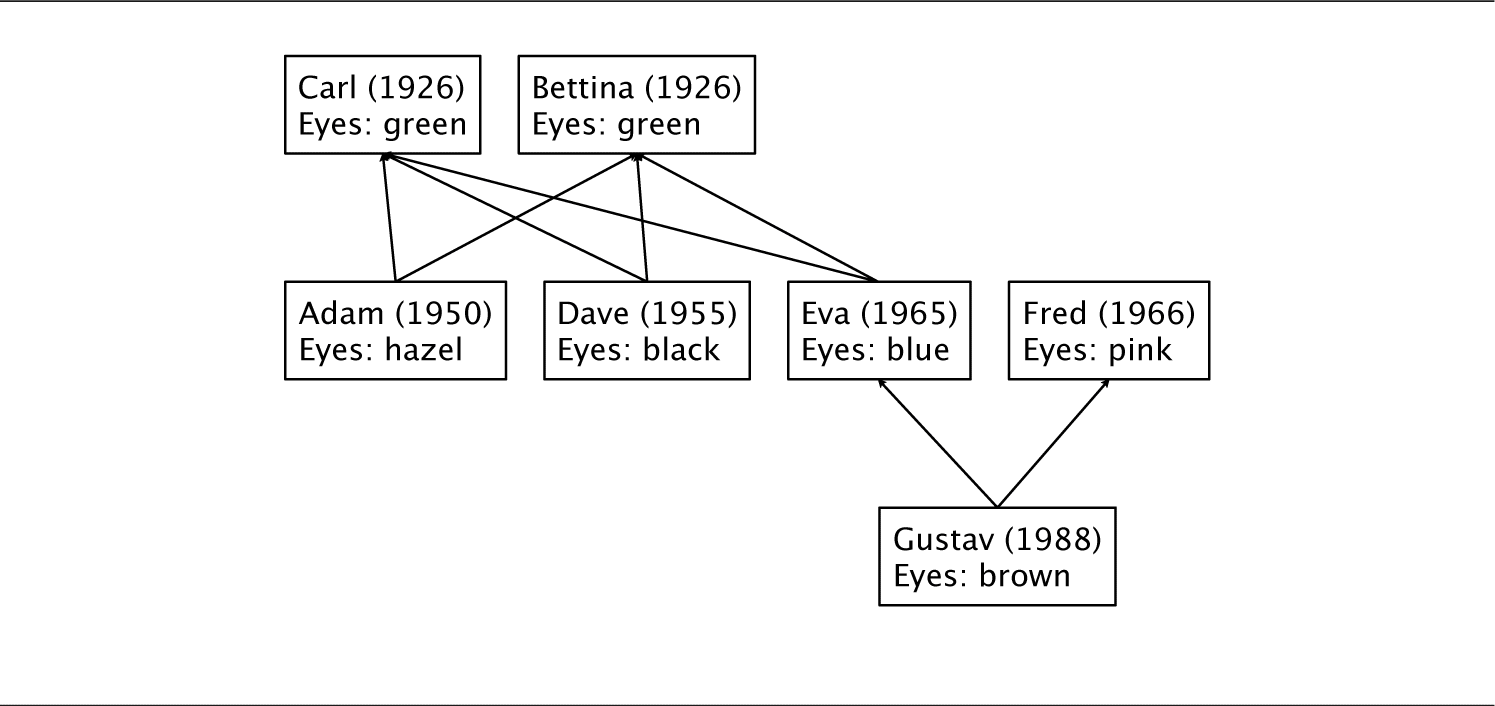
\includegraphics[width=0.85\textwidth]{images/00450.png}
  \caption{家谱图 (A family tree)}
  \label{fig:111}
\end{figure}

一旦家谱规模庞大，将其表示为程序中的数据并设计能够处理此类数据的程序就变得顺理成章。鉴于家谱中的一个节点汇集了五项信息——父亲、母亲、姓名、出生年份以及眼睛颜色——我们应当定义一个结构体类型：

\begin{lstlisting}[language=BSL]
(define-struct child [father mother name date eyes])
\end{lstlisting}

该结构体类型的定义自然引导出一份数据定义：

\begin{lstlisting}[language=BSL]
; Child 是一个结构体：
;   (make-child Child Child String N String)
\end{lstlisting}

虽然这份数据定义看起来非常直观，但它实际上是\textbf{无法使用}的。它引用了自身，然而由于它没有任何基本分支（clause），我们根本无法构造出一个合法的 \code{Child} 实例。简言之，我们必须无休止地写下去：

\begin{lstlisting}[language=BSL]
(make-child (make-child (make-child ...) ...) ...)
\end{lstlisting}

这将陷入无限循环。为了避免这种无意义的数据定义，我们要求\textbf{自引用数据定义必须包含多个分支，且其中至少有一个分支不回引该数据定义自身}。

让我们暂时搁置数据定义的最终定稿，先通过实验来探索。假设我们要向现有的家谱中添加一个孩子，且父母的表示已经存在。在这种情况下，我们只需构建一个新的 \code{child} 结构体。例如，在已经表示了 Carl 与 Bettina 的程序中，要表示 Adam，只需添加如下结构体：

\begin{lstlisting}[language=BSL]
(define Adam
  (make-child Carl Bettina "Adam" 1950 "hazel"))
\end{lstlisting}

这里假定 \code{Carl} 与 \code{Bettina} 代表 Adam 父母的家谱表示。

然而，某个人的父母可能是未知的，就像图~\ref{fig:111} 中 Bettina 的父母那样。即便如此，在 \code{child} 表示中，我们依然必须为相应的父母字段填充值。无论我们选择什么数据，它都必须明确表达\textbf{信息的缺失}。一方面，我们可以从现有值池中选用 \code{\#false}、\code{"none"} 或 \code{'()}；另一方面，我们更应当明确宣称：该信息在当前家谱中不存在。通过引入一个命名恰当的结构体类型，可以最优雅地达成这一目标：

\begin{lstlisting}[language=BSL]
(define-struct no-parent [])
\end{lstlisting}

现在，为了为 Bettina 构建一个 \code{child} 结构体，我们可以这样写：

\begin{lstlisting}[language=BSL]
(make-child (make-no-parent) (make-no-parent) "Bettina" 1926 "green")
\end{lstlisting}

当然，如果只有一方父母信息缺失，我们就只需在对应字段中填入这一特殊值。

上述实验为我们带来了两点深刻见解：
\begin{enumerate}
  \item 我们寻求的不是一个描述如何生成单个 \code{child} 结构体实例的数据定义，而是一个描述\textbf{如何表示完整家谱}的数据定义。
  \item 该数据定义包含两个分支：一个分支描述未知的家谱，另一个分支描述已知的家谱。
\end{enumerate}

\begin{lstlisting}[language=BSL]
(define-struct no-parent [])
(define-struct child [father mother name date eyes])

; 一个 FT（Family Tree，家谱）是下列之一：
; -- (make-no-parent)
; -- (make-child FT FT String N String)
\end{lstlisting}

由于表示“无父母”的树在程序中频繁出现，我们定义 \code{NP} 作为简写，并略微修饰数据定义：

\begin{lstlisting}[language=BSL]
(define NP (make-no-parent))

; 一个 FT 是下列之一：
; -- NP
; -- (make-child FT FT String N String)
\end{lstlisting}

遵循第 9 章的设计配方，我们利用数据定义来创建家谱的数据样例。具体而言，我们将图~\ref{fig:111} 中的家谱翻译为数据表示。Carl 的信息很容易翻译：

\begin{lstlisting}[language=BSL]
(make-child NP NP "Carl" 1926 "green")
\end{lstlisting}

Bettina 和 Fred 也用类似的 \code{child} 实例表示。而 Adam 则需要嵌套子节点，分别对应 Carl 和 Bettina：

\begin{lstlisting}[language=BSL]
(make-child (make-child NP NP "Carl" 1926 "green")
            (make-child NP NP "Bettina" 1926 "green")
            "Adam"
            1950
            "hazel")
\end{lstlisting}

由于 Carl 和 Bettina 的记录在构建 Dave 和 Eva 时也需要用到，更好的做法是引入变量定义来命名特定的 \code{child} 实例，并在其他地方引用这些变量名。图~\ref{fig:112} 展示了图~\ref{fig:111} 完整家谱的数据表示。请仔细观察这棵树，它将作为后续设计练习的持续案例。

\begin{figure}[htbp]
  \centering
\begin{lstlisting}[language=BSL, basicstyle=\scriptsize\ttfamily]
; Oldest Generation:
(define Carl (make-child NP NP "Carl" 1926 "green"))
(define Bettina (make-child NP NP "Bettina" 1926 "green"))

; Middle Generation:
(define Adam (make-child Carl Bettina "Adam" 1950 "hazel"))
(define Dave (make-child Carl Bettina "Dave" 1955 "black"))
(define Eva (make-child Carl Bettina "Eva" 1965 "blue"))
(define Fred (make-child NP NP "Fred" 1966 "pink"))

; Youngest Generation:
(define Gustav (make-child Fred Eva "Gustav" 1988 "brown"))
\end{lstlisting}
  \caption{样本家谱的数据表示 (A data representation of the sample family tree)}
  \label{fig:112}
\end{figure}

在设计具体的家谱处理函数之前，我们先来看看此类函数的通用组织结构。换句话说，在尚未确定具体任务的情况下，尽可能推进设计配方的步骤。我们从设计配方的第二步（签名、目的说明与函数头）开始：

\begin{lstlisting}[language=BSL]
; FT -> ???
; ...
(define (fun-FT an-ftree)
  ...)
\end{lstlisting}

虽然我们尚未陈述函数的具体目的，但已知它接收一个家谱作为主要输入。签名中的 \code{???} 表明输出类型未定，省略号则提醒我们目的尚待明确。

缺乏具体目的意味着我们无法编写具体的功能示例。然而，我们完全可以依据 \code{FT} 的数据定义结构来设计模板。由于 \code{FT} 包含两个分支，模板必须包含一个含有两个条件分支的 \code{cond} 表达式：

\begin{lstlisting}[language=BSL]
(define (fun-FT an-ftree)
  (cond
    [(no-parent? an-ftree) ...]
    [(child? an-ftree) ...]))
\end{lstlisting}

当输入满足 \code{no-parent?} 时，该结构不包含任何附加数据，因此第一个分支处理完毕。对于第二个分支，输入包含五项数据，我们在模板中用五个选择器表达式标明：

\begin{lstlisting}[language=BSL]
(define (fun-FT an-ftree)
  (cond
    [(no-parent? an-ftree) ...]
    [else
     (... (child-father an-ftree) ...
      ... (child-mother an-ftree) ...
      ... (child-name an-ftree) ...
      ... (child-date an-ftree) ...
      ... (child-eyes an-ftree) ...)]))
\end{lstlisting}

模板构造的最后一步涉及\textbf{自引用}。如果数据定义引用了自身，函数极有可能发生递归，模板通过启发性的自然递归调用体现这一点。\code{FT} 的定义包含两处自引用（父亲与母亲字段均是 \code{FT}），因此模板需要两处自然递归：

\begin{lstlisting}[language=BSL]
(define (fun-FT an-ftree)
  (cond
    [(no-parent? an-ftree) ...]
    [else
     (... (fun-FT (child-father an-ftree)) ...
      ... (fun-FT (child-mother an-ftree)) ...
      ... (child-name an-ftree) ...
      ... (child-date an-ftree) ...
      ... (child-eyes an-ftree) ...)]))
\end{lstlisting}

具体来说，在第二个 \code{cond} 分支中，\code{fun-FT} 分别作用于父亲与母亲的数据表示，因为数据定义的第二个分支恰恰包含了这两处对 \code{FT} 的自引用。

现在让我们转向一个具体问题：设计 \code{blue-eyed-child?} 函数。该函数的目的是确定给定家谱中是否存在眼睛颜色为蓝色的孩子。我们可以复制、粘贴并重命名 \code{fun-FT} 来获得模板，将 \code{???} 替换为 \code{Boolean} 并添加目的说明：

\begin{lstlisting}[language=BSL]
; FT -> Boolean
; 判断给定家谱中是否包含蓝眼睛的孩子
(define (blue-eyed-child? an-ftree)
  (cond
    [(no-parent? an-ftree) ...]
    [else
     (... (blue-eyed-child? (child-father an-ftree)) ...
      ... (blue-eyed-child? (child-mother an-ftree)) ...
      ... (child-name an-ftree) ...
      ... (child-date an-ftree) ...
      ... (child-eyes an-ftree) ...)]))
\end{lstlisting}

根据设计配方，我们回溯到用例设计步骤。如果以 Carl 开始，Carl 的眼睛是 \code{"green"}，其祖先树均为空，因此 Carl 的家谱中绝不可能有蓝眼睛的孩子：

\begin{lstlisting}[language=BSL]
(check-expect (blue-eyed-child? Carl) #false)
\end{lstlisting}

相反，Gustav 的母亲 Eva 拥有蓝眼睛：

\begin{lstlisting}[language=BSL]
(check-expect (blue-eyed-child? Gustav) #true)
\end{lstlisting}

现在我们准备填充函数体。函数区分两种情形：\code{no-parent} 和 \code{child}。对于第一种情形，家谱为空，自然不可能包含蓝眼睛的孩子，因此结果为 \code{\#false}。

对于第二种情形，依据设计配方，我们首先明确模板中各个表达式的作用：
\begin{enumerate}
  \item \code{(blue-eyed-child? (child-father an-ftree))} 判断父亲一方的家谱中是否有蓝眼睛的孩子；
  \item \code{(blue-eyed-child? (child-mother an-ftree))} 判断母亲一方的家谱中是否有蓝眼睛的孩子；
  \item 选择器表达式 \code{(child-name an-ftree)}、\code{(child-date an-ftree)} 和 \code{(child-eyes an-ftree)} 分别提取当前孩子的姓名、出生年份和眼睛颜色。
\end{enumerate}

显然，如果当前孩子的眼睛字段为 \code{"blue"}，函数直接返回 \code{\#true}。姓名和出生年份对于判断眼睛颜色无用。剩下的问题是如何组合这三个布尔表达式：如果当前孩子是蓝眼睛，或者父亲一方有蓝眼睛，或者母亲一方有蓝眼睛，则整棵家谱中就存在蓝眼睛：

\begin{lstlisting}[language=BSL]
(or (string=? (child-eyes an-ftree) "blue")
    (blue-eyed-child? (child-father an-ftree))
    (blue-eyed-child? (child-mother an-ftree)))
\end{lstlisting}

图~\ref{fig:113} 给出了完整的函数定义。

\begin{figure}[htbp]
  \centering
\begin{lstlisting}[language=BSL, basicstyle=\scriptsize\ttfamily]
; FT -> Boolean
; does an-ftree contain a child
; structure with "blue" in the eyes field

(check-expect (blue-eyed-child? Carl) #false)
(check-expect (blue-eyed-child? Gustav) #true)

(define (blue-eyed-child? an-ftree)
  (cond
    [(no-parent? an-ftree) #false]
    [else (or (string=? (child-eyes an-ftree) "blue")
              (blue-eyed-child? (child-father an-ftree))
              (blue-eyed-child? (child-mother an-ftree)))]))
\end{lstlisting}
  \caption{在祖先树中寻找蓝眼睛的孩子 (Finding a blue-eyed child in an ancestor tree)}
  \label{fig:113}
\end{figure}

由于这是本书中第一个使用双重递归调用的函数，图~\ref{fig:114} 模拟了单步求值器对 \code{(blue-eyed-child? Carl)} 的求值轨迹，帮助你体会树形递归的运作机制。

\begin{figure}[htbp]
  \centering
\begin{lstlisting}[language=BSL, basicstyle=\scriptsize\ttfamily]
1. (child-eyes (make-child NP NP "Carl" 1926 "green"))
   ==
   "green"

2. (blue-eyed-child?
     (child-father
       (make-child NP NP "Carl" 1926 "green")))
   ==
   (blue-eyed-child? NP)
   ==
   #false

3. (blue-eyed-child?
     (child-mother
       (make-child NP NP "Carl" 1926 "green")))
   ==
   (blue-eyed-child? NP)
   ==
   #false
\end{lstlisting}
  \caption{树结构的求值推导计算 (Calculating with trees)}
  \label{fig:114}
\end{figure}

\begin{exercise}{统计家谱中的人数}{310}
开发函数 \code{count-persons}。该函数接收一棵家谱 \code{FT}，统计树中包含的 \code{child} 结构体的总数。
\end{exercise}

\begin{exercise}{计算家谱中的平均年龄}{311}
开发函数 \code{average-age}。该函数接收一棵家谱与当前年份，计算家谱中所有 \code{child} 结构体所代表人物的平均年龄。
\end{exercise}

\begin{exercise}{收集家谱中的眼睛颜色}{312}
开发函数 \code{eye-colors}。该函数接收一棵家谱，生成该树中出现的所有眼睛颜色的列表。某种眼睛颜色在结果列表中可多次出现。\emph{提示：} 使用 \code{append} 拼接递归调用返回的列表。
\end{exercise}

\begin{exercise}{寻找蓝眼睛祖先}{313}
假设我们需要函数 \code{blue-eyed-ancestor?}。它与 \code{blue-eyed-child?} 类似，但仅当给定孩子的\textbf{真正祖先}（即不包含该孩子本人）拥有蓝眼睛时才返回 \code{\#true}。

请首先为该函数编写签名与目的说明：
\begin{lstlisting}[language=BSL]
; FT -> Boolean
(define (blue-eyed-ancestor? an-ftree)
  ...)
\end{lstlisting}

为了理解其区别，以 Eva 为例：Eva 本人是蓝眼睛，但她没有蓝眼睛的祖先：
\begin{lstlisting}[language=BSL]
(check-expect (blue-eyed-child? Eva) #true)
(check-expect (blue-eyed-ancestor? Eva) #false)
\end{lstlisting}
而 Gustav 是 Eva 的儿子，他确实拥有蓝眼睛祖先：
\begin{lstlisting}[language=BSL]
(check-expect (blue-eyed-ancestor? Gustav) #true)
\end{lstlisting}

现在假设一位朋友提出了如下解法：
\begin{lstlisting}[language=BSL]
(define (blue-eyed-ancestor? an-ftree)
  (cond
    [(no-parent? an-ftree) #false]
    [else
     (or (blue-eyed-ancestor? (child-father an-ftree))
         (blue-eyed-ancestor? (child-mother an-ftree)))]))
\end{lstlisting}
解释为什么该函数无法通过测试。无论传入什么家谱，该函数的返回值都是什么？你能修复这位朋友的解法吗？
\end{exercise}

\section{森林 }
\label{sec:19.2_forests}

从家谱走向“家庭森林”（Family Forest，简称森林）仅有一步之遥：

\begin{lstlisting}[language=BSL]
; 一个 FF（family forest，家族森林）是下列之一：
; -- '()
; -- (cons FT FF)
; 解释：家族森林表示若干个家族（例如一个城镇中的居民）及其祖先树
\end{lstlisting}

以下是从图~\ref{fig:111} 中摘取的若干树构成的森林示例：

\begin{lstlisting}[language=BSL]
(define ff1 (list Carl Bettina))
(define ff2 (list Fred Eva))
(define ff3 (list Fred Eva Carl))
\end{lstlisting}

前两个森林包含互不相关的家族，第三个则说明：与自然界的森林不同，家族森林中的树木在逻辑上是可以相互重叠的。

现在考虑如下典型问题：

\begin{notebox}[样本问题]
设计函数 \code{blue-eyed-child-in-forest?}，判断给定的家族森林中是否包含眼睛为 \code{"blue"} 的孩子。
\end{notebox}

图~\ref{fig:115} 展示了该问题的直观解法。森林本质上是一个列表，因此可以沿用列表模板。如果列表的每一项都是带有眼睛字段的单一结构体，函数只需遍历这些结构体并进行比较。而在本例中，列表的每一项都是一棵完整的家谱树，幸运的是，我们已经掌握了如何处理家谱树（直接复用 \code{blue-eyed-child?}）。

\begin{figure}[htbp]
  \centering
\begin{lstlisting}[language=BSL, basicstyle=\scriptsize\ttfamily]
; FF -> Boolean
; does the forest contain any child with "blue" eyes

(check-expect (blue-eyed-child-in-forest? ff1) #false)
(check-expect (blue-eyed-child-in-forest? ff2) #true)
(check-expect (blue-eyed-child-in-forest? ff3) #true)

(define (blue-eyed-child-in-forest? a-forest)
  (cond
    [(empty? a-forest) #false]
    [else
     (or (blue-eyed-child? (first a-forest))
         (blue-eyed-child-in-forest? (rest a-forest)))]))
\end{lstlisting}
  \caption{在家族森林中寻找蓝眼睛的孩子 (Finding a blue-eyed child in a family forest)}
  \label{fig:115}
\end{figure}

退一步审视图~\ref{fig:115} 的构成。起点是一对数据定义，其中第二个定义引用了第一个，且两者各自包含自引用。结果是一对相互配合的函数定义：第二个函数调用了第一个，且两者各自递归。换句话说，\textbf{函数定义之间的相互引用关系完全镜像了数据定义之间的相互引用关系}。早先章节对这种关系略有涉及，但现在这种结构已足够丰富，值得给予充分的关注。

\begin{exercise}{使用 List-of 抽象重构森林定义}{314}
使用 \code{List-of} 抽象重新表述 \code{FF} 的数据定义。然后对 \code{blue-eyed-child-in-forest?} 做同样的重构。最后，使用前一章学过的列表抽象函数（例如 \code{ormap}）来重新定义 \code{blue-eyed-child-in-forest?}。
\end{exercise}

\begin{exercise}{计算森林中人员的平均年龄}{315}
设计函数 \code{average-age}。该函数接收一个家族森林与一个年份（\code{N}），计算森林中所有 \code{child} 实例的平均年龄。
\emph{注意：} 如果森林中的树存在重叠，直接求和可能导致某些人被重复计算；在本练习中，暂且假设森林中的各棵树互不重叠。
\end{exercise}

\section{S-表达式 }
\label{sec:19.3_sexpr}

虽然插曲 2 非正式地介绍了 S-表达式（S-expression），但我们可以通过三个互相交织的数据定义精确描述它们：

\begin{lstlisting}[language=BSL]
; 一个 S-expr（S-表达式）是下列之一：
; -- Atom
; -- SL

; 一个 SL（S-表达式列表）是下列之一：
; -- '()
; -- (cons S-expr SL)

; 一个 Atom（原子）是下列之一：
; -- Number
; -- String
; -- Symbol
\end{lstlisting}

请回忆：符号（Symbol）在书写时形如单引号开头的字符串，末尾不加引号，例如 \code{'hello}。

S-表达式的思想源自约翰·麦卡锡（John McCarthy）及其 Lisp 团队，他们在 1958 年发明了 S-表达式，以便能够\textbf{用 Lisp 程序来处理 Lisp 程序}。这种看似循环的构想听起来十分玄妙，但正如插曲 2 所述，S-表达式是一种极具通用性的数据形态，屡屡被后人重新发现，最近的大规模应用便是万维网（XML/HTML 与 JSON）。掌握 S-表达式将为我们设计高度交织的数据定义及其处理函数打下坚实基础。

\begin{exercise}{定义 atom? 谓词}{316}
在 BSL 中定义 \code{atom?} 谓词函数，判断给定值是否属于 \code{Atom}。
\end{exercise}

在此之前，本书中尚未出现过像 S-表达式这样复杂的数据定义。然而，只要遵循扩展后的设计配方，你完全能够设计出处理 S-表达式的函数。我们通过一个具体问题来展示这一点：

\begin{notebox}[样本问题]
设计函数 \code{count}，统计某个给定符号在某 S-表达式中出现的总次数。
\end{notebox}

第一步是创建数据样例。S-表达式的定义指出每个 \code{Atom} 都是 \code{S-expr}：
\begin{lstlisting}[language=BSL]
'hello
20.12
"world"
\end{lstlisting}

同样，每个 \code{SL} 既是一个列表，也是一个 \code{S-expr}：
\begin{lstlisting}[language=BSL]
'()
(cons 'hello (cons 20.12 (cons "world" '())))
(cons (cons 'hello (cons 20.12 (cons "world" '()))) '())
\end{lstlisting}

借助插曲 2 的引用（quote）机制，书写 S-表达式变得极为便捷。我们在 DrRacket 交互区中验证这些例子：

\begin{replbox}
> '()
'()
> '(hello 20.12 "world")
(list 'hello #i20.12 "world")
> '((hello 20.12 "world"))
(list (list 'hello #i20.12 "world"))
\end{replbox}

借助 \code{quote}，我们还可以轻松构造形如代码或数据表格的复杂表达式：

\begin{replbox}
> '(define (f x) (+ x 10))
(list 'define (list 'f 'x) (list '+ 'x 10))
> '((mercury 1) (venus 2) (earth 3))
(list (list 'mercury 1) (list 'venus 2) (list 'earth 3))
> '(wing (wing body wing) wing)
(list 'wing (list 'wing 'body 'wing) 'wing)
\end{replbox}

现在为 \code{count} 写出函数头与功能示例：

\begin{lstlisting}[language=BSL]
; S-expr Symbol -> N
; 统计 sy 在 sexp 中出现的总次数
(check-expect (count 'world 'hello) 0)
(check-expect (count '(world hello) 'hello) 1)
(check-expect (count '(((world) hello) hello) 'hello) 2)

(define (count sexp sy)
  0)
\end{lstlisting}

在模板设计阶段，面对相互交织的数据定义，我们需要核心设计准则：

\begin{notebox}[交织数据模板准则]
对于互相交织的数据定义，\textbf{为每个数据定义各创建一个模板}。并行创建它们，并确保模板之间的调用关系与数据定义之间的引用关系完全对应。
\end{notebox}

对于当前问题，我们需要三个模板：
\begin{enumerate}
  \item \code{count}：处理 \code{S-expr}；
  \item \code{count-sl}：处理 \code{SL}；
  \item \code{count-atom}：处理 \code{Atom}。
\end{enumerate}

图~\ref{fig:116} 给出了这三个完整的函数模板。模板之间的调用箭头精确复刻了数据定义之间的引用箭头。

\begin{figure}[htbp]
  \centering
\begin{stepperbox}[unbreakable]
\noindent\begin{minipage}[t]{0.48\linewidth}\vspace{0pt}
\begin{Verbatim}[fontsize=\fontsize{6.0pt}{7.2pt}\selectfont]
(define (count sexp sy)
  (cond
    [(atom? sexp)
     (count-atom sexp sy)]
    [else
     (count-sl sexp sy)]))

(define (count-sl sl sy)
  (cond
    [(empty? sl) ...]
    [else
     (...
      (count (first sl) sy)
      ...
      (count-sl (rest sl) sy)
      ...)]))
\end{Verbatim}
\end{minipage}\hfill
\noindent\begin{minipage}[t]{0.48\linewidth}\vspace{0pt}
\begin{Verbatim}[fontsize=\fontsize{6.0pt}{7.2pt}\selectfont]
(define (count-atom at sy)
  (cond
    [(number? at) ...]
    [(string? at) ...]
    [(symbol? at) ...]))
\end{Verbatim}
\end{minipage}
\end{stepperbox}
  \caption{S-表达式的处理模板 (A template for S-expressions)}
  \label{fig:116}
\end{figure}

在这些模板的基础上填补空白，便得到了图~\ref{fig:117} 中的完整程序。

\begin{figure}[htbp]
  \centering
\begin{lstlisting}[language=BSL, basicstyle=\scriptsize\ttfamily]
; S-expr Symbol -> N
; counts all occurrences of sy in sexp
(define (count sexp sy)
  (cond
    [(atom? sexp) (count-atom sexp sy)]
    [else (count-sl sexp sy)]))

; SL Symbol -> N
; counts all occurrences of sy in sl
(define (count-sl sl sy)
  (cond
    [(empty? sl) 0]
    [else
     (+ (count (first sl) sy) (count-sl (rest sl) sy))]))

; Atom Symbol -> N
; counts all occurrences of sy in at
(define (count-atom at sy)
  (cond
    [(number? at) 0]
    [(string? at) 0]
    [(symbol? at) (if (symbol=? at sy) 1 0)]))
\end{lstlisting}
  \caption{S-表达式的计数程序 (A program for S-expressions)}
  \label{fig:117}
\end{figure}

让我们逐一审视各个关键分支：
\begin{itemize}
  \item \code{[(atom? sexp) (count-atom sexp sy)]}：若 \code{sexp} 是原子，则转交专职函数 \code{count-atom} 处理；
  \item \code{[else (+ (count (first sl) sy) (count-sl (rest sl) sy))]}：列表由第一项（一个 \code{S-expr}）和其余项（一个 \code{SL}）组成，分别调用对应函数统计后相加；
  \item \code{[(symbol? at) (if (symbol=? at sy) 1 0)]}：若原子是符号且与目标符号相等，则计数为 1，否则为 0。
\end{itemize}

\begin{exercise}{使用 local 整合多函数}{317}
由三个互相关联的函数组成的程序，理应使用 \code{local} 表达式体现这种从属关系。

请将图~\ref{fig:117} 中的程序重组为包含内部辅助函数的单个 \code{count} 函数。由于第二个参数 \code{sy} 在整个遍历过程中从不改变，你可以从局部辅助函数的参数列表中移除它，从而向读者表明 \code{sy} 是遍历过程中的全局常量。
\end{exercise}

\begin{exercise}{计算 S-表达式的深度}{318}
设计函数 \code{depth}。该函数接收一个 S-表达式并计算其嵌套深度。\code{Atom} 的深度为 1。S-表达式列表的深度为其各元素深度的最大值加 1。空列表的深度可视为 0 或 1（请明确你的约定）。
\end{exercise}

\begin{exercise}{S-表达式的符号替换}{319}
设计函数 \code{substitute}。它接收一个 S-表达式 \code{s} 以及两个符号 \code{old} 和 \code{new}。其结果与 \code{s} 相同，只是其中所有出现的 \code{old} 均被替换为 \code{new}。
\end{exercise}

\begin{exercise}{重构并化简 S-expr 定义}{320}
重新表述 \code{S-expr} 的数据定义，将第一个分支直接展开为 \code{Atom} 的三个分支，并在第二个分支中使用 \code{[List-of S-expr]} 抽象。针对这一新定义重新设计 \code{count} 函数。你能否结合 \code{lambda} 进一步化简该函数？
\end{exercise}

\begin{exercise}{对 S-表达式中的原子进行抽象}{321}
对 \code{S-expr} 和 \code{SL} 的数据定义进行参数化抽象，使其能够容纳不同种类的原子数据。
\end{exercise}

\section{交织数据的设计 }
\label{sec:19.4_intertwined_recipe}

从自引用数据定义跃升到相互引用的复合数据定义集合，其跨度远比从固定数据跨越到自引用数据要小。第 9 章的设计配方只需微调即可直接适用于此：

\begin{figure}[htbp]
  \centering
  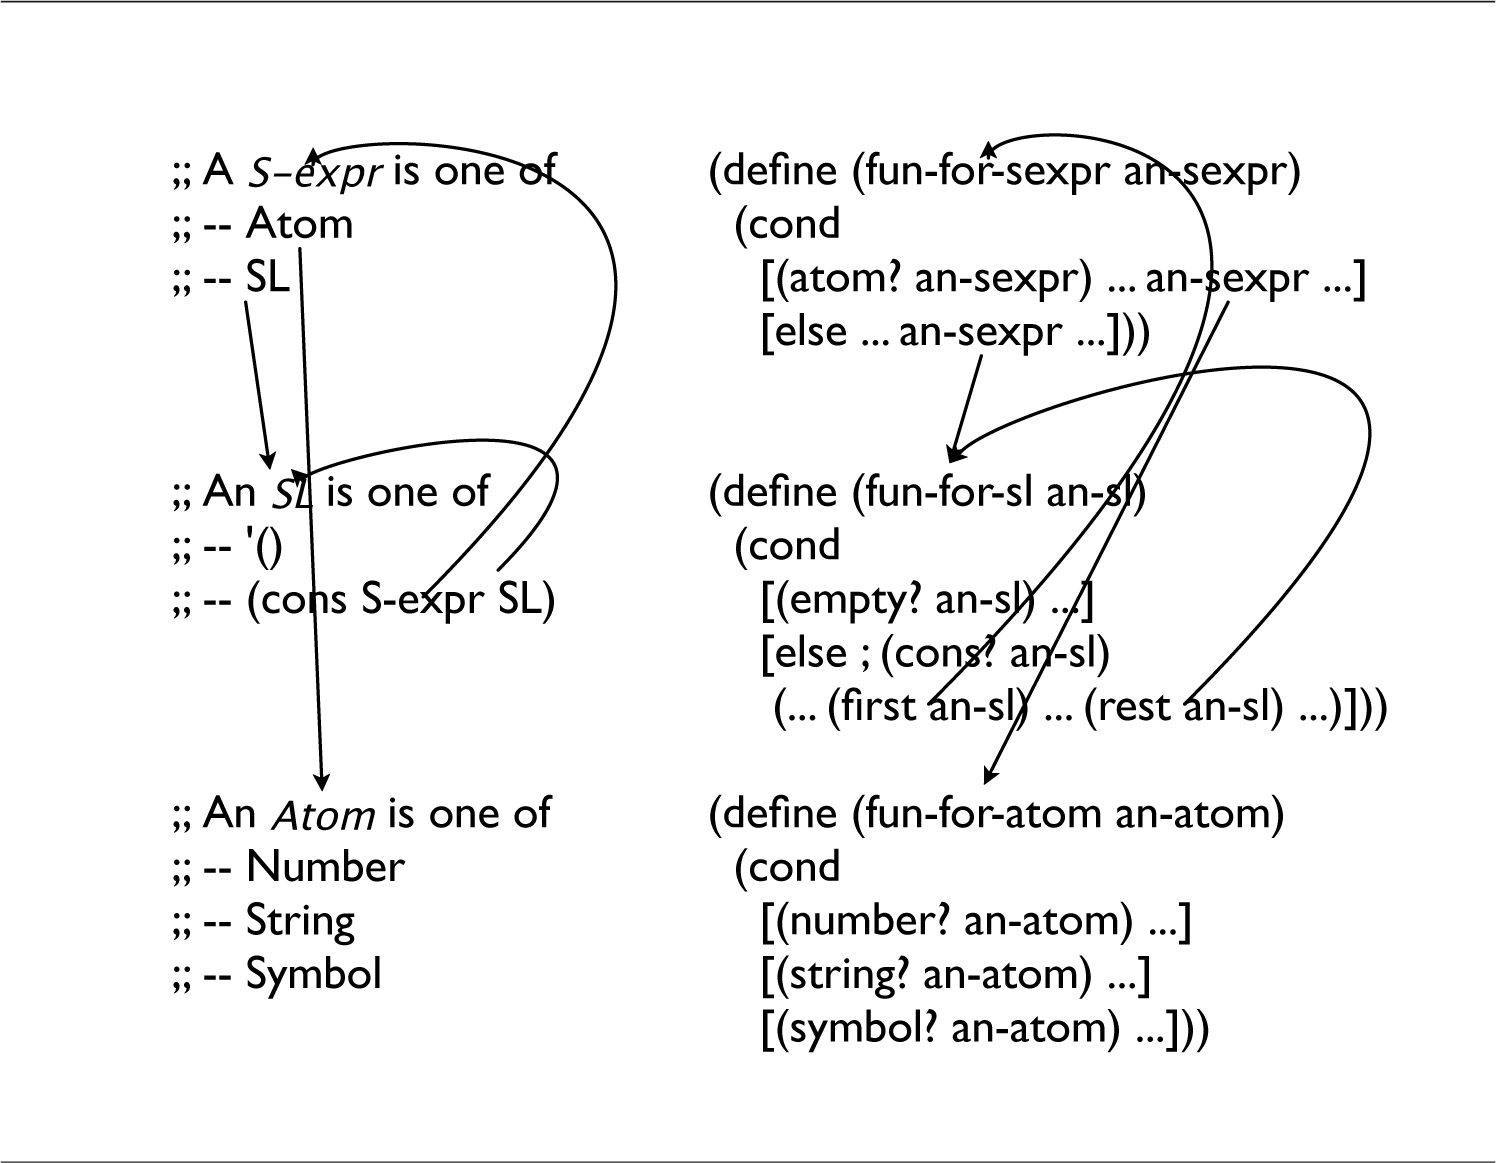
\includegraphics[width=0.85\textwidth]{images/00472.png}
  \caption{数据定义与模板间的引用关系对应 (Arrows for nests of data definitions and templates)}
  \label{fig:118}
\end{figure}

\begin{recipebox}[交织数据与相互递归函数的设计配方]
\textbf{1. 数据定义：} 当问题涉及多种不同形态的信息且相互嵌套时，编写一组互相引用的数据定义。画出各个定义之间的引用箭头（见图~\ref{fig:118} 左侧）。确保为每个定义都能构造出合法的基本用例。

\textbf{2. 签名与函数头：} 数据定义集合中有多少个数据定义，就\textbf{并行设计多少个函数}。每个函数专职处理其中一种数据定义，其余公共参数保持不变。

\textbf{3. 功能示例：} 构造测试用例，确保覆盖各定义之间的所有相互引用路径。

\textbf{4. 模板设计：} 为每个函数依据其主要输入的数据定义设计模板。数据定义中每出现一个指向其他定义的箭头，模板中就对应画出一个函数调用箭头（见图~\ref{fig:118} 右侧）。最终将箭头替换为具体的函数调用。

\textbf{5. 填充函数体：} 首先解决基准情形（不含递归或跨函数调用的分支），然后处理自引用和相互递归分支。

\textbf{6. 测试与排错：} 运行测试。若某个辅助函数存在缺陷，可能会同时引发主函数与辅助函数的报错。修复该辅助函数即可同时解决两处故障。
\end{recipebox}




\label{sec:ch19_more_trees}

程序员常常利用树形数据结构来显著提升函数的执行性能。其中一种格外著名的树形结构是\term{二叉搜索树}（Binary Search Tree，简称 BST），因为它是快速存储和检索海量信息的经典方案。

\section{项目：二叉搜索树 }
\label{sec:19.5_bsts}

具体而言，我们讨论用于管理人事信息的二叉树。与家谱中的 \code{child} 结构体不同，二叉树由节点（node）构成：

\begin{lstlisting}[language=BSL]
(define-struct no-info [])
(define NONE (make-no-info))

(define-struct node [ssn name left right])

; 一个 BT（Binary Tree，二叉树）是下列之一：
; -- NONE
; -- (make-node Number Symbol BT BT)
\end{lstlisting}

相应的数据定义与家谱树非常相似：\code{NONE} 表示信息的缺失，每个 \code{node} 记录一个社会安全号（SSN，作为唯一的数字标识）、一个姓名以及另外两棵二叉树（左子树与右子树）。后两者类似于家谱中的父母，只是节点与其左右子树的关系不再基于血缘亲属，而是基于某种组织次序。

图~\ref{fig:119} 展示了如何用图形方式来理解这些树。在计算机科学中，树通常是倒着画的：根节点（root）在最顶端，树冠与树叶在最底部。每个圆圈对应一个节点，圆圈内的数字标明对应 \code{node} 结构体的 \code{ssn} 字段。在绘图中，\code{NONE} 通常被省略。

\begin{figure}[htbp]
  \centering
  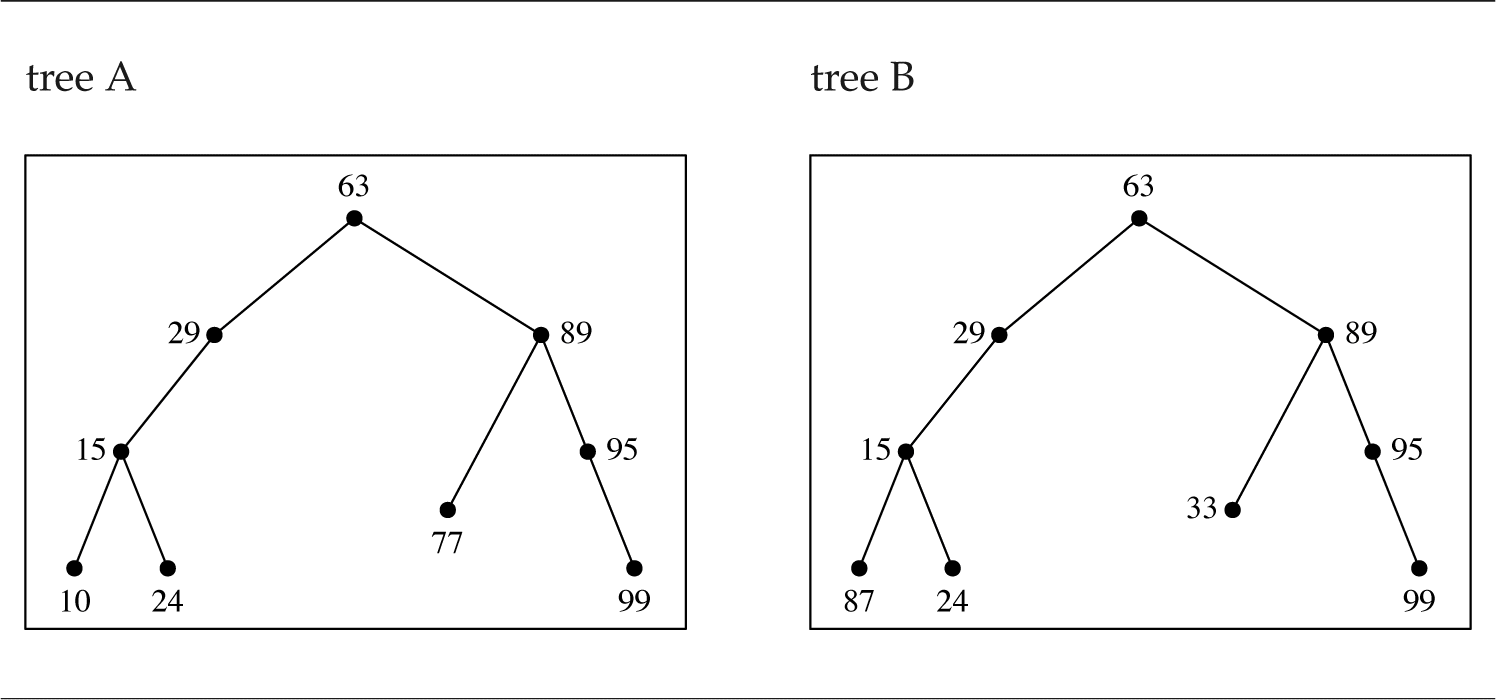
\includegraphics[width=0.85\textwidth]{images/00474.png}
  \caption{二叉搜索树与普通二叉树 (A binary search tree and a binary tree)}
  \label{fig:119}
\end{figure}

\begin{exercise}{绘制二叉树并设计 contains-bt?}{322}
按照图~\ref{fig:119} 的风格画出题目中给出的样本二叉树。然后设计函数 \code{contains-bt?}，判断给定的数字是否出现在某个给定的二叉树 \code{BT} 中。
\end{exercise}

\begin{exercise}{在二叉树中搜索指定社保号}{323}
设计函数 \code{search-bt}。该函数接收一个数字 \code{n} 与一棵二叉树 \code{BT}。若树中包含 \code{ssn} 为 \code{n} 的节点，则返回该节点的 \code{name} 字段值；否则返回 \code{\#false}。

\emph{提示：} 可以先调用 \code{contains-bt?} 检查整棵树，或者在每一步自然递归后使用 \code{boolean?} 检查递归结果。
\end{exercise}

如果我们从左向右读取图~\ref{fig:119} 中两棵树的所有数字，将得到两个不同的序列：
\begin{itemize}
  \item 树 A 的读取结果为：\code{(list 10 15 24 29 63 77 89 95 99)}
  \item 树 B 的读取结果为：\code{(list 15 24 10 29 95 63 89 77 99)}
\end{itemize}

树 A 的序列是严格升序排列的，而树 B 则不是。第一类具有有序性质的二叉树正是\term{二叉搜索树}（BST）。每一棵二叉搜索树都是二叉树，但并非每一棵二叉树都是二叉搜索树。更确切地说，我们可以表述区分二叉搜索树与普通二叉树的核心数据不变量：

\begin{notebox}[二叉搜索树不变量 (The BST Invariant)]
一棵 \term{BST} 是满足如下约束条件的 \code{BT}：
\begin{itemize}
  \item \code{NONE} 永远是一棵 BST；
  \item \code{(make-node ssn0 name0 L R)} 是一棵 BST，当且仅当：
  \begin{enumerate}
    \item \code{L} 是一棵 BST；
    \item \code{R} 是一棵 BST；
    \item \code{L} 中的所有 \code{ssn} 字段均\textbf{小于} \code{ssn0}；
    \item \code{R} 中的所有 \code{ssn} 字段均\textbf{大于} \code{ssn0}。
  \end{enumerate}
\end{itemize}
\end{notebox}

换言之，要验证一棵普通二叉树是否是二叉搜索树，我们必须检查所有子树中的数值，确保它们严格小于或大于当前节点的键值。这一不变量在构建数据时增加了一定约束，但在数据检索时将带来巨大的性能优势。

\begin{exercise}{二叉树的中序遍历 inorder}{324}
设计函数 \code{inorder}。该函数接收一棵二叉树，产生从左到右遍历树图时所见的所有 \code{ssn} 组成的列表。

\emph{提示：} 使用 \code{append} 拼接列表：
\begin{lstlisting}[language=BSL]
(append (list 1 2 3) (list 4) (list 5 6 7)) == (list 1 2 3 4 5 6 7)
\end{lstlisting}
思考：对一棵二叉搜索树执行 \code{inorder} 会产生什么样的列表？
\end{exercise}

在二叉搜索树中查找特定社保号的节点时，我们可以充分利用 BST 不变量。在普通二叉树中，为了确认某个数字是否存在，函数可能不得不遍历整棵树的每一个节点。相比之下，在二叉搜索树中，函数每访问一个节点，就可以果断\textbf{排除掉两棵子树中的一整棵}：

假设我们在如下样本 BST 中查找目标：
\begin{lstlisting}[language=BSL]
(make-node 66 'a L R)
\end{lstlisting}
如果目标是 66，查找成功。若目标小于 66（例如 63），我们只需聚焦于左子树 \code{L}，因为所有小于 66 的节点都在 \code{L} 中。反之，若目标是 99，我们可以完全忽略 \code{L}，直接在右子树 \code{R} 中查找。

\begin{exercise}{在二叉搜索树中高效查找 search-bst}{325}
设计函数 \code{search-bst}。该函数接收数字 \code{n} 与一棵二叉搜索树 \code{BST}。若树中包含 \code{ssn} 为 \code{n} 的节点，产生其 \code{name} 字段值；否则产生 \code{NONE}。函数组织结构必须利用 BST 不变量，使得执行的比较次数尽可能少。回顾第 189 题中有序列表的二分查找思想并进行对比！
\end{exercise}

构建一棵普通二叉树非常简单；但构建一棵二叉搜索树则需要缜密的逻辑。随意将两个 BST 和一个新数拼接，通常无法得到合法的 BST。

\begin{exercise}{向 BST 中插入节点 create-bst}{326}
设计函数 \code{create-bst}。该函数接收一个二叉搜索树 \code{B}、一个数字 \code{N} 以及一个符号 \code{S}。它生成一棵新的二叉搜索树，其内容与 \code{B} 相同，只是在恰当的 \code{NONE} 叶子位置插入了新节点：
\begin{lstlisting}[language=BSL]
(make-node N S NONE NONE)
\end{lstlisting}
设计完成后，在图~\ref{fig:119} 中的树 A 上测试该函数。
\end{exercise}

\begin{exercise}{从列表批量构建 BST}{327}
设计函数 \code{create-bst-from-list}。它接收一个由数与姓名组成的列表，通过反复调用 \code{create-bst} 从中构造出一棵完整的二叉搜索树。其函数签名如下：
\begin{lstlisting}[language=BSL]
; [List-of (list Number Symbol)] -> BST
\end{lstlisting}
使用该函数处理样本输入序列，验证是否能构造出图~\ref{fig:119} 中的树 A。如果你使用现有的列表折叠抽象（如 \code{foldr}），可能会得到一棵镜像“反转”的树，为什么？
\end{exercise}

\section{简化函数结构}
\label{sec:19.6_simplifying}

练习 317 展示了如何使用 \code{local} 来组织处理交织数据的多函数程序。当我们确定数据定义已经定型后，这种组织结构还能帮助我们大幅度精简代码。为了阐明这一点，我们展示如何系统性地化简练习 319 中 \code{substitute} 函数的实现。

图~\ref{fig:120} 展示了 \code{substitute} 的完整初始定义。该定义严格按照数据定义的要求，使用 \code{local} 声明了三个辅助函数，并附带了测试用例。

\begin{figure}[htbp]
  \centering
\begin{lstlisting}[language=BSL, basicstyle=\scriptsize\ttfamily]
; S-expr Symbol Atom -> S-expr
; replaces all occurrences of old in sexp with new

(check-expect (substitute '(((world) bye) bye) 'bye '42)
              '(((world) 42) 42))

(define (substitute sexp old new)
  (local (; S-expr -> S-expr
          (define (for-sexp sexp)
            (cond
              [(atom? sexp) (for-atom sexp)]
              [else (for-sl sexp)]))
          ; SL -> S-expr
          (define (for-sl sl)
            (cond
              [(empty? sl) '()]
              [else (cons (for-sexp (first sl))
                          (for-sl (rest sl)))]))
          ; Atom -> S-expr
          (define (for-atom at)
            (cond
              [(number? at) at]
              [(string? at) at]
              [(symbol? at) (if (equal? at old) new at)])))
    (for-sexp sexp)))
\end{lstlisting}
  \caption{待化简的 S-表达式替换程序 (A program to be simplified)}
  \label{fig:120}
\end{figure}

\begin{exercise}{验证待化简程序}{328}
将图~\ref{fig:120} 复制到 DrRacket 中，补充充分的测试用例并运行。在阅读本节后续内容时，同步修改代码并重新运行测试套件，以验证每一步化简的等价性。
\end{exercise}

\textbf{第一步化简：利用现有抽象。} 鉴于 \code{SL} 本质上是 \code{S-expr} 的列表，我们可以使用高阶函数 \code{map} 极大简化 \code{for-sl}。原程序说明 \code{for-sexp} 作用于 \code{sl} 的每一项，使用 \code{map} 能更精准清晰地表达这一意图（见图~\ref{fig:121}）。

\begin{figure}[htbp]
  \centering
\begin{lstlisting}[language=BSL, basicstyle=\scriptsize\ttfamily]
(define (substitute sexp old new)
  (local (; S-expr -> S-expr
          (define (for-sexp sexp)
            (cond
              [(atom? sexp) (for-atom sexp)]
              [else (for-sl sexp)]))
          ; SL -> S-expr
          (define (for-sl sl)
            (map for-sexp sl))
          ; Atom -> S-expr
          (define (for-atom at)
            (cond
              [(number? at) at]
              [(string? at) at]
              [(symbol? at) (if (equal? at old) new at)])))
    (for-sexp sexp)))
\end{lstlisting}
  \caption{程序化简第一步：引入 map (Program simplification, step 1)}
  \label{fig:121}
\end{figure}

\textbf{第二步化简：通用相等比较。} 我们注意到 \code{equal?} 能够直接比较任意两个数据值。因此，第三个局部函数 \code{for-atom} 实际上可以精简为一行表达式。图~\ref{fig:122} 展示了这第二阶段的简化。

\begin{figure}[htbp]
  \centering
\begin{lstlisting}[language=BSL, basicstyle=\scriptsize\ttfamily]
(define (substitute sexp old new)
  (local (; S-expr -> S-expr
          (define (for-sexp sexp)
            (cond
              [(atom? sexp) (for-atom sexp)]
              [else (for-sl sexp)]))
          ; SL -> S-expr
          (define (for-sl sl) (map for-sexp sl))
          ; Atom -> S-expr
          (define (for-atom at)
            (if (equal? at old) new at)))
    (for-sexp sexp)))

(define (substitute.v3 sexp old new)
  (local (; S-expr -> S-expr
          (define (for-sexp sexp)
            (cond
              [(atom? sexp)
               (if (equal? sexp old) new sexp)]
              [else
               (map for-sexp sexp)])))
    (for-sexp sexp)))
\end{lstlisting}
  \caption{程序化简第二与第三步 (Program simplification, steps 2 and 3)}
  \label{fig:122}
\end{figure}

\textbf{第三步化简：函数内联与 lambda。} 此时，最后两个局部定义都只有一行代码，且两者都不包含递归。因此，我们可以将它们直接\term{内联}（in-line）到 \code{for-sexp} 中：将 \code{(for-atom sexp)} 替换为 \code{(if (equal? sexp old) new sexp)}；对于 \code{(for-sl sexp)}，直接替换为 \code{(map for-sexp sexp)}。

经过这一系列内联与提炼，整个程序最终可以优雅地浓缩为一个高度精炼的单函数结构：

\begin{lstlisting}[language=BSL]
; S-expr Symbol Symbol -> S-expr
; 将 sexp 中所有出现的 old 替换为 new
(define (substitute sexp old new)
  (cond
    [(atom? sexp) (if (equal? sexp old) new sexp)]
    [else
     (map (lambda (s) (substitute s old new)) sexp)]))
\end{lstlisting}

观察上述最终形态：原本三个互递归函数、数十行样板代码，最终化为如此清澈、兼具表现力与数学美感的五行定义。这就是掌握交织数据与高阶抽象后的程序之美！

% ==============================================================================
% 第 20 章：逐步求精 (Chapter 20: Iterative Refinement)
% ==============================================================================

\chapter{逐步求精}
\label{sec:ch20_refinement}

当你着手开发面向真实世界的程序时，往往需要面对极其复杂的信息形态，以及如何用程序数据来精确刻画这些信息的问题。应对这一挑战的最佳策略是采用\term{逐步求精}（iterative refinement）——这是科学探索中久经考验的方法论。

科学家的核心任务是使用某种数学形式来描述客观世界的一部分，这种努力的产物被称为\term{模型}（model）。随后，科学家通过各种方式测试模型，尤其是预测实验的结果。如果预测值与实际测量值之间的偏差过大，科学家就会精炼改进该模型，以提高预测的精度。这一迭代过程持续进行，直到预测足够准确为止。

考虑一位希望预测火箭飞行轨迹的物理学家：起初将“火箭视为质点”的模型固然简单，但也非常粗糙，因为它完全无法解释空气阻力。为此，物理学家随后加入了火箭的几何外形，并引入必要的空气动力学方程来计算阻力——这第二个模型就是对第一个模型的精炼。通过反复迭代，预测精度逐步收敛到令人满意的程度。

计算机科学专业的程序员也应当像这位物理学家一样工作。其核心在于找到现实世界信息的精准数据表示，并设计能够恰当处理这些数据的函数。复杂场景要求我们经历由简入繁的精炼过程，从最核心的信息要素出发，逐步添加细节。有时，在程序交付部署后，因用户提出新需求，程序员也必须对模型实施进一步的精炼。

到目前为止，我们在遇到复杂数据形态时已多次在幕后为你运用了逐步求精。本章将以一个综合性案例——计算机文件系统（目录树）的建模与处理——来系统演示作为程序开发核心原则的逐步求精。我们将探讨文件系统的本质，并逐步迭代构建出三个层层深入的数据表示。

\section{数据分析 }
\label{sec:20.1_data_analysis}

在关闭计算机或退出 DrRacket 之前，你必须确保你的所有工作都已安全保存，否则下次启动时就必须重头再来。因此，你让计算机将程序和数据存入\term{文件}（file）中。从抽象视角看，文件大体上可以看作是一段字符串（在底层则是连续的字节序列）。

在现代操作系统中，文件被组织在\term{目录}（directory，通常也称文件夹 folder）之中。简而言之，一个目录包含若干个文件以及若干个更深层的目录。后者被称为\term{子目录}（sub-directory），子目录内部又可以嵌套包含更多的子目录与文件。基于这种层次化结构，我们称之为\term{目录树}（directory tree）。

图~\ref{fig:123} 展示了一个小型的目录树示意图。与计算机科学中常见的“根节点在上”的画法不同，本图按照自然界树木的生长方向自底向上绘制：根目录名为 \code{TS}。根目录下包含一个名为 \code{read!} 的文件，以及名为 \code{Text} 和 \code{Libs} 的两个子目录。\code{Text} 目录下仅包含 3 个文件；而 \code{Libs} 目录下包含两个子目录，每个子目录下又包含各自的文件。每个方框右上角标明了类型属性：目录标记为 \code{DIR}，文件则标记为其大小（以整数表示所占字节或存储单位）。

\begin{figure}[htbp]
  \centering
  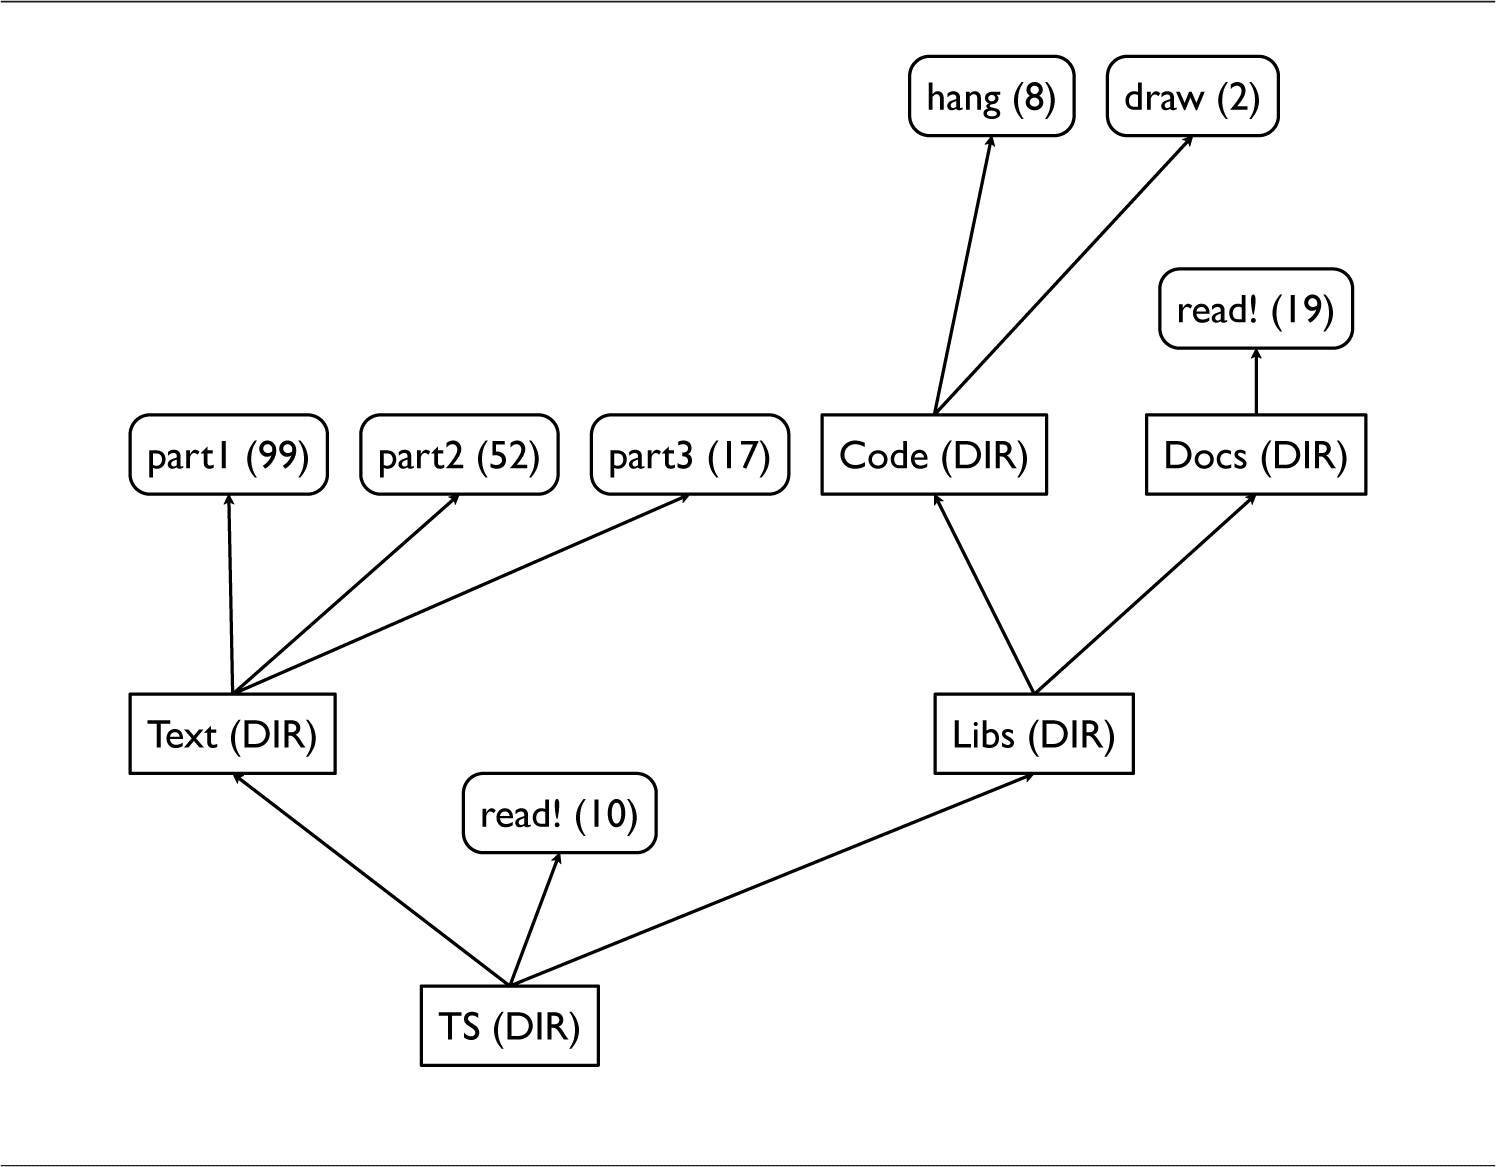
\includegraphics[width=0.85\textwidth]{images/00481.png}
  \caption{样本目录树 TS (A sample directory tree)}
  \label{fig:123}
\end{figure}

\begin{exercise}{分析样本目录树 TS}{329}
观察图~\ref{fig:123} 中的目录树 \code{TS}：
\begin{enumerate}
  \item 名为 \code{read!} 的文件在整棵树中共出现了多少次？你能写出从根目录到各次出现的完整路径吗？
  \item 该目录树中所有文件的总大小是多少？
  \item 若每个目录节点本身也占用 1 个单位的存储空间，整个目录树的总开销是多少？
  \item 该目录树共嵌套了多少层目录？
\end{enumerate}
\end{exercise}

\section{逐步细化数据定义}
\label{sec:20.2_refining_data}

练习 329 列举了用户对文件系统日常提出的典型查询。操作系统内核提供了各种命令来解答这些问题。为了设计类似的程序，我们必须建立目录树的数据表示。

我们在本节通过三次迭代，逐步提炼出三个数据模型。在每个阶段，我们权衡包含哪些属性，抽象忽略哪些细节。

\subsection{模型 1：文件为原子，目录为容器}

在最简视角下，用户将文件视为具有名字的原子实体，而将目录单纯视为容纳文件与其他目录的“容器”。基于此，我们将目录表示为列表，将文件表示为字符串（即文件名）：

\begin{lstlisting}[language=BSL]
; 一个 Dir.v1（目录版本 1）是下列之一：
; -- '()
; -- (cons File.v1 Dir.v1)
; -- (cons Dir.v1 Dir.v1)

; 一个 File.v1 是一个 String。
\end{lstlisting}

后缀 \code{.v1} 用于区分后续的精炼版本。

\begin{exercise}{将目录树表示为模型 1 数据}{330}
根据模型 1 的数据定义，将图~\ref{fig:123} 中的目录树 \code{TS} 翻译为 BSL 数据表示。
\end{exercise}

\begin{exercise}{统计模型 1 中的文件数}{331}
设计函数 \code{how-many}，统计给定 \code{Dir.v1} 中包含的文件总数。请严格遵循设计配方，并利用练习 330 的数据用例进行测试。
\end{exercise}

\subsection{模型 2：引入具名目录结构体}

模型 1 虽然简单，但抹杀了目录的重要本质——在模型 1 中，目录自身没有名字！我们无法列出某目录下所有子目录的名称。为了更忠实地反映现实，我们必须引入一个将“名称”与“内容容器”结合起来的结构体类型：

\begin{lstlisting}[language=BSL]
(define-struct dir [name content])

; 一个 Dir.v2 是一个结构体：
;   (make-dir String LOFD)

; 一个 LOFD（List-of-Files-and-Directories，文件与目录列表）是下列之一：
; -- '()
; -- (cons File.v2 LOFD)
; -- (cons Dir.v2 LOFD)

; 一个 File.v2 是一个 String。
\end{lstlisting}

请注意：\code{Dir.v2} 引用了 \code{LOFD}，而 \code{LOFD} 又回引了 \code{Dir.v2}。这是一对\textbf{相互递归}的数据定义。

\begin{exercise}{将目录树表示为模型 2 数据}{332}
根据模型 2 的数据定义，将图~\ref{fig:123} 中的目录树 \code{TS} 翻译为数据表示。
\end{exercise}

\begin{exercise}{统计模型 2 中的文件数}{333}
设计函数 \code{how-many}，统计给定 \code{Dir.v2} 中包含的文件总数。将你的函数实现与练习 331 进行对比。
\end{exercise}

\begin{exercise}{扩展目录属性：大小与可读性}{334}
展示如何为目录结构体增加两个属性：大小（size，衡量目录元数据自身所占的空间）与可读性（readability，指定除所有者外的其他人是否可以浏览该目录内容）。给出相应的结构体定义与数据定义。
\end{exercise}

\subsection{模型 3：文件属性与子项拆分}

现实中的文件不仅有文件名，还包含文件大小、修改日期与内容。我们为文件定义专用的结构体：

\begin{lstlisting}[language=BSL]
(define-struct file [name size content])

; 一个 File.v3 是一个结构体：
;   (make-file String N String)
\end{lstlisting}

同时，在目录结构体中，将“文件列表”与“子目录列表”清晰地分开存放，不仅逻辑更分明，处理起来也更加模块化：

\begin{lstlisting}[language=BSL]
(define-struct dir.v3 [name dirs files])

; 一个 Dir.v3 是一个结构体：
;   (make-dir.v3 String Dir* File*)

; 一个 Dir* 是下列之一：
; -- '()
; -- (cons Dir.v3 Dir*)

; 一个 File* 是下列之一：
; -- '()
; -- (cons File.v3 File*)
\end{lstlisting}

按照计算机科学传统，名称末尾加 \code{*}（星号）表示“多个”，以区分单数实体 \code{Dir.v3} 与复数集合 \code{Dir*}。

\begin{exercise}{将目录树表示为模型 3 数据}{335}
按照模型 3 的数据定义，将图~\ref{fig:123} 中的目录树 \code{TS} 转换为数据表示，文件内容统一使用空字符串 \code{""}。
\end{exercise}

\begin{exercise}{统计模型 3 中的文件数}{336}
设计函数 \code{how-many}，统计给定 \code{Dir.v3} 中包含的文件总数。面对高度复杂的相互递归数据定义，你为什么能够坚信自己的函数计算结果是完全正确的？
\end{exercise}

\begin{exercise}{使用 List-of 抽象与高阶函数重构}{337}
利用 \code{List-of} 抽象重新定义 \code{Dir.v3}：
\begin{lstlisting}[language=BSL]
(define-struct dir.v3 [name dirs files])
; 一个 Dir.v3 是：(make-dir.v3 String [List-of Dir.v3] [List-of File.v3])
\end{lstlisting}
随后利用 ISL+ 中的列表高阶处理函数（如 \code{foldr}、\code{map}），重新实现练习 336 中的 \code{how-many}。
\end{exercise}

\section{逐步细化函数}
\label{sec:20.3_refining_functions}

为了使后续练习更具实战感，DrRacket 提供了 \code{htdp/dir} 教学库。该库内置了模型 3 的结构体定义（去掉了 \code{.v3} 后缀），并提供了一个能够直接读取你电脑真实目录树的函数：

\begin{lstlisting}[language=BSL]
(require htdp/dir)

; String -> Dir
; 读取路径 a-path 所指的真实目录，生成对应的 Dir 数据表示
(define (create-dir a-path) ...)
\end{lstlisting}

例如，在定义区输入并运行：
\begin{lstlisting}[language=BSL]
(define O (create-dir "/Users/matthias/")) ; OS X
(define L (create-dir "/var/log/"))        ; Linux
(define W (create-dir "C:\\Users\\..."))    ; Windows
\end{lstlisting}
你就能获得本地磁盘的真实目录数据结构！

\begin{notebox}[使用注意]
1. 对于非常庞大的目录树，DrRacket 构建数据表示可能需要较长时间。请首先在小型文件夹上试验。\\
2. \textbf{不要}在代码中自行用 \code{define-struct} 定义 \code{dir} 和 \code{file}，因为引入教学包后二次定义会导致命名冲突。
\end{notebox}

在后续练习中，路径（Path）被表示为由目录和文件名构成的字符串列表：
\begin{lstlisting}[language=BSL]
; 一个 Path 是一个 [List-of String]
; 解释：指引进入目录树深处的路径导航序列
\end{lstlisting}
例如在图~\ref{fig:123} 中，从根目录 \code{TS} 到 \code{part1} 的路径为 \code{(list "TS" "Text" "part1")}。

\begin{exercise}{在真实文件系统上运行 how-many}{338}
利用 \code{create-dir} 将你电脑上的某个目录转化为数据表示，然后调用练习 336 中的 \code{how-many} 统计其文件数。借助系统自带的文件管理器验证其准确性。
\end{exercise}

\begin{exercise}{搜索指定文件是否存在 find?}{339}
设计函数 \code{find?}。该函数接收一个 \code{Dir} 与一个文件名，判断该目录树中是否存在具有该名称的文件。
\end{exercise}

\begin{exercise}{列出所有文件与目录名 ls}{340}
设计函数 \code{ls}，列出给定 \code{Dir} 及其所有嵌套子目录中包含的所有文件和目录的名字列表。
\end{exercise}

\begin{exercise}{计算目录总占用空间 du}{341}
设计函数 \code{du}，接收一个 \code{Dir} 并计算其整棵目录树占用的总存储空间。假设存储每个目录节点本身固定消耗 1 个单位空间。
\end{exercise}

\begin{exercise}{查找文件的完整路径 find}{342}
设计函数 \code{find}。该函数接收目录 \code{d} 与文件名 \code{f}。若该文件存在，返回通往该文件的路径；若不存在，返回 \code{\#false}。

\emph{进阶挑战：} 图~\ref{fig:123} 中有两个名为 \code{read!} 的文件，基本的 \code{find} 通常只能返回其中一条路径。设计函数 \code{find-all}，返回所有能够找到 \code{f} 的路径列表。
\end{exercise}

\begin{exercise}{递归列出所有文件的完整路径 ls-R}{343}
设计函数 \code{ls-R}，列出给定目录树中所有文件的完整路径列表。
\end{exercise}

\begin{exercise}{组合式设计重构 find-all}{344}
使用练习 343 中的 \code{ls-R} 重新设计练习 342 中的 \code{find-all}。这就是通过函数组合（design by composition）解决复杂问题的高阶范式。
\end{exercise}

% ==============================================================================
% 第 21 章：解释器的精炼 (Chapter 21: Refining Interpreters)
% ==============================================================================

\chapter{解释器的精炼}
\label{sec:ch21_interpreters}

DrRacket 本身就是一个程序。它是一个极其复杂的软件，处理着许多形态各异的数据。如同大多数大型软件系统一样，DrRacket 由许多模块和函数组成：有的负责让程序员编辑文本代码，有的负责驱动交互区（Interactions Area），有的负责检查定义的语法合法性等等。

在本章中，我们将向你展示如何设计\textbf{驱动交互区核心运作的函数}。毫无疑问，我们在这个综合设计项目中依然采用\term{逐步求精}。实际上，聚焦于 DrRacket 的这一核心功能本身就是逐步求精思想的体现——先实现最关键的计算核心。

简而言之，交互区的核心职责是：\textbf{计算你在提示符后输入的表达式的值}。当你点击 \textsf{RUN}（运行）按钮后，交互区加载定义区中的所有常量和函数定义。随后，它随时准备接收你输入的可能引用了这些定义的表达式，计算求出该表达式的值，并将结果打印出来，而后周而复始。正因如此，人们通常将交互区称为\term{REPL}（Read-Eval-Print Loop，读取-求值-打印循环）。其中 \term{eval} 是求值器（evaluator）的缩写，在计算机科学中更通用的称谓是\term{解释器}（interpreter）。

我们的精炼流程从最基础的 BSL 数值算术表达式出发；它们结构简单，不依赖复杂的环境定义，易于推演。一旦你理清了第一步，就能深刻领会“BSL 表达式自身”与其“在程序中的数据表示（AST）”之间的根本区别。随后，我们引入变量，最后一步引入函数定义与函数调用。

\section{解释算术表达式 }
\label{sec:21.1_eval_expr}

我们的首要任务是建立 BSL 表达式的数据表示。换句话说，我们必须弄清楚如何将一段 BSL 表达式本身表示为 BSL 语言内部的一项数据。乍听之下这有些不可思议（用语言自身表示自身的代码），但其实非常直观。

假设我们起初只想表示数字、加法与乘法。数值本身可以直接表示数值。加法表达式则是一种复合数据，因为它由两个子表达式和一个操作符组成；乘法表达式亦然。

遵循第 5 章的方法，最直接的表示方式是定义两个各自拥有两个字段的结构体类型：

\begin{lstlisting}[language=BSL]
(define-struct add [left right])
(define-struct mul [left right])
\end{lstlisting}

其语义是：\code{left} 字段保存左操作数，\code{right} 字段保存右操作数。下表列出了三组对照关系：
\begin{center}
\begin{tabular}{lll}
\hline
\textbf{BSL 代码} & \textbf{含义} & \textbf{在 BSL 中的数据表示} \\
\hline
\code{3} & 数值 3 & \code{3} \\
\code{(+ 1 2)} & 加法 & \code{(make-add 1 2)} \\
\code{(* 2 3)} & 乘法 & \code{(make-mul 2 3)} \\
\hline
\end{tabular}
\end{center}

对于包含嵌套子表达式的表达式，例如：
\begin{lstlisting}[language=BSL]
(+ (* 3 3) (* 4 4))
\end{lstlisting}
结构体字段可以容纳任意深度嵌套的数据表示：
\begin{lstlisting}[language=BSL]
(make-add (make-mul 3 3) (make-mul 4 4))
\end{lstlisting}
图~\ref{fig:124} 给出了更多样例对照。

\begin{figure}[htbp]
  \centering
\begin{stepperbox}[unbreakable]
\centering\scriptsize\ttfamily
\begin{tabular}{@{}l@{\hspace{8pt}}l@{}}
\toprule
{\normalfont\bfseries BSL expression} & {\normalfont\bfseries representation of BSL expression} \\
\midrule
(+ (* 1 1) 10) & (make-add (make-mul 1 1) 10) \\
\addlinespace
(+ (* 3 3) & (make-add (make-mul 3 3) \\
\phantom{(+ }(* 4 4)) & \phantom{(make-add }(make-mul 4 4)) \\
\addlinespace
(+ (* (+ 1 2) 3) & (make-add (make-mul (make-add 1 2) 3) \\
\phantom{(+ }(* (* (+ 1 1) & \phantom{(make-add }(make-mul (make-mul \\
\phantom{(+ (* (* }2) & \phantom{(make-add (make-mul (make-}(make-add 1 1) \\
\phantom{(+ (* }4)) & \phantom{(make-add (make-mul (make-add 1 }2) \\
 & \phantom{(make-add (make-mul (make-mul }4)) \\
\bottomrule
\end{tabular}
\end{stepperbox}
  \caption{在 BSL 中表示 BSL 表达式 (Representing BSL expressions in BSL)}
  \label{fig:124}
\end{figure}

\begin{exercise}{BSL 表达式的数据定义与表示}{345}
基于 \code{add} 与 \code{mul} 结构体，给出 BSL 算术表达式的数据定义，将此类数据命名为 \code{BSL-expr}。
\begin{enumerate}
  \item 将下列 BSL 表达式翻译为其数据表示：
  \begin{itemize}
    \item \code{(+ 10 -10)}
    \item \code{(+ (* 20 3) 33)}
    \item \code{(+ (* 3.14 (* 2 3)) (* 3.14 (* -1 -9)))}
  \end{itemize}
  \item 将下列数据表示还原为人类可读的 BSL 表达式：
  \begin{itemize}
    \item \code{(make-add -1 2)}
    \item \code{(make-add (make-mul -2 -3) 33)}
    \item \code{(make-mul (make-add 1 (make-mul 2 3)) 3.14)}
  \end{itemize}
\end{enumerate}
\end{exercise}

有了表达式的数据表示后，下一步是设计求值器 \code{eval-expression}。该函数接收一个 \code{BSL-expr} 并计算出它的最终数值。

\begin{exercise}{表达式计算结果值的数据定义}{346}
为 \code{BSL-expr} 求值后所产生的结果值集合制定数据定义（对于目前的纯算术表达式，该集合即为所有的数 \code{Number}）。
\end{exercise}

\begin{exercise}{设计算术求值器 eval-expression}{347}
设计函数 \code{eval-expression}。该函数接收一个 \code{BSL-expr}，递归计算并返回其数值。
\end{exercise}

\begin{exercise}{布尔表达式的表示与求值}{348}
设计布尔 BSL 表达式的数据表示，支持 \code{\#true}、\code{\#false}、\code{and}、\code{or} 与 \code{not}。随后设计求值函数 \code{eval-bool-expression} 计算其布尔结果。
\end{exercise}

\subsection{语法解析：从 S-表达式到解析树}

直接手写层层嵌套的结构体（如 \code{make-add}、\code{make-mul}）非常繁琐。幸运的是，S-表达式提供了一种更贴近真实语法的输入方式：只需在代码前加上一个单引号，例如 \code{'(+ (* 3 3) (* 4 4))}，DrRacket 就会将其作为嵌套列表与符号读入！

然而，S-表达式过于宽泛（例如 \code{"hello"} 或 \code{'(+ 1 2 3 4)} 都是 S-表达式，但不符合简单二元表达式的语法）。为了架起便捷书写与严谨内部结构体之间的桥梁，程序员发明了\term{语法解析器}（parser）。解析器负责检查输入是否合乎语法规则；若合法，则构建出内部的\term{解析树}（parse tree，即我们的结构体表示）；若不合法，则抛出语法错误。

图~\ref{fig:125} 给出了一个将 S-表达式解析为 \code{BSL-expr} 的解析器 \code{parse}。

\begin{figure}[htbp]
  \centering
\begin{lstlisting}[language=BSL, basicstyle=\scriptsize\ttfamily]
; S-expr -> BSL-expr
(define (parse s)
  (cond
    [(atom? s) (parse-atom s)]
    [else (parse-sl s)]))

; SL -> BSL-expr
(define (parse-sl s)
  (local ((define L (length s)))
    (cond
      [(< L 3) (error WRONG)]
      [(and (= L 3) (symbol? (first s)))
       (cond
         [(symbol=? (first s) '+)
          (make-add (parse (second s)) (parse (third s)))]
         [(symbol=? (first s) '*)
          (make-mul (parse (second s)) (parse (third s)))]
         [else (error WRONG)])]
      [else (error WRONG)])))

; Atom -> BSL-expr
(define (parse-atom s)
  (cond
    [(number? s) s]
    [(string? s) (error WRONG)]
    [(symbol? s) (error WRONG)]))
\end{lstlisting}
  \caption{从 S-表达式到 BSL 解析树 (From S-expr to BSL-expr)}
  \label{fig:125}
\end{figure}

\begin{exercise}{解析器 parse 的完整测试套件}{349}
为图~\ref{fig:125} 中的 \code{parse} 编写充分的测试用例，确保在 DrRacket 运行测试时代码覆盖率达到 100\%。
\end{exercise}

\begin{exercise}{解析器的非常规设计分析}{350}
从设计配方的角度审视图~\ref{fig:125} 的程序组织：它有哪些不同寻常之处？（例如对列表长度的检查）。
\end{exercise}

\begin{exercise}{设计直接面向 S-表达式的求值器}{351}
设计函数 \code{interpreter-expr}。该函数接收一个 S-表达式，若 \code{parse} 将其识别为合法的 \code{BSL-expr}，则调用求值器返回其计算值；否则抛出与 \code{parse} 相同的语法错误。
\end{exercise}

\section{解释变量 }
\label{sec:21.2_eval_variables}

上一节排除了变量定义。然而在实际编程中，定义区通常包含常量定义，例如：
\begin{lstlisting}[language=BSL]
(define x 5)
(define y 3)
\end{lstlisting}
而在交互区中，表达式往往包含这些变量名：
\begin{replbox}
> (+ x 3)
8
> (* 1/2 (* x y))
7.5
\end{replbox}

为了支持变量，我们必须扩展数据表示：变量以符号（Symbol）表示。

\begin{lstlisting}[language=BSL]
; 一个 BSL-var-expr 是下列之一：
; -- Number
; -- Symbol
; -- (make-add BSL-var-expr BSL-var-expr)
; -- (make-mul BSL-var-expr BSL-var-expr)
\end{lstlisting}

\subsection{代换模型 }

在初等代数中，求含变量表达式的值的方法是：\textbf{将所有变量替换为其所代表的具体数值}。在纯函数式语言中，这种方法完全有效。

\begin{exercise}{变量代换函数 subst}{352}
设计函数 \code{subst}。该函数接收一个 \code{BSL-var-expr ex}、一个符号 \code{x} 和一个数值 \code{v}。它生成一个新的表达式，将 \code{ex} 中所有出现的变量 \code{x} 全部替换为数值 \code{v}。
\end{exercise}

\begin{exercise}{检查表达式是否为纯数值 numeric?}{353}
设计函数 \code{numeric?}，判断给定的 \code{BSL-var-expr} 是否已不包含任何变量（即是否蜕变为纯算术表达式 \code{BSL-expr}）。
\end{exercise}

为了支持多个常量定义，我们引入\term{关联列表}（Association List，简称 AL）来表示定义区中的所有变量与数值的绑定：

\begin{lstlisting}[language=BSL]
; 一个 AL（Association List，关联列表）是 [List-of Association]。
; 一个 Association 是一个包含两项的列表：
;    (list Symbol Number)
\end{lstlisting}

\begin{exercise}{变量求值器与关联列表}{354}
设计函数 \code{eval-variable}，接收一个 \code{BSL-var-expr}。若输入满足 \code{numeric?}，则计算其值；否则报错“未绑定变量”。

进而设计函数 \code{eval-variable*}。该函数接收一个表达式 \code{ex} 和一个关联列表 \code{da}（表示常量环境），依次对关联列表中的每对绑定调用 \code{subst} 进行全局代换，最后调用 \code{eval-variable} 获得计算结果。
\end{exercise}

\subsection{环境模型 }

代换模型在计算开始前对整个 AST 树实施全量扫描与替换。另一种更符合现代计算机工业实现的方案是\term{环境模型}（environment model）：在求值过程中随身携带包含变量绑定的环境（即关联列表 \code{da}）。解释器每当在表达式树中遇到一个变量符号时，便即时在环境中查找该符号的值并加以使用。

\begin{exercise}{基于环境模型的变量求值 eval-var-lookup}{355}
设计函数 \code{eval-var-lookup}：
\begin{lstlisting}[language=BSL]
; BSL-var-expr AL -> Number
(define (eval-var-lookup e da) ...)
\end{lstlisting}
该函数不采用预先代换，而是在深度优先遍历表达式树的同时“随身携带”关联列表 \code{da}。当遇到符号 \code{x} 时，使用 \code{assq} 在 \code{da} 中查找其绑定值；若未找到，则抛出未定义变量错误。
\end{exercise}

\section{解释函数 }
\label{sec:21.3_eval_functions}

掌握了常量与变量后，精炼的下一个关键目标是：\textbf{支持程序员自定义的函数及其调用}。

为降低复杂度，我们首先假定定义区中的所有函数均只接收一个参数。在代数中，函数定义形如 $f(x) = e$，函数调用形如 $f(a)$。对其求值的步骤是：先求出实参 $a$ 的值，再将函数体 $e$ 中的形参 $x$ 替换为该实参值，最后对替换后的函数体求值。

\begin{exercise}{包含函数调用的表达式数据定义}{356}
扩展表达式的数据表示以支持单参函数调用。函数调用包含两项信息：被调用的函数名（Symbol）与传入的实参表达式（\code{BSL-fun-expr}）。定义结构体 \code{(define-struct app [name arg])}，并将此类扩展后的数据命名为 \code{BSL-fun-expr}。
\end{exercise}

\begin{exercise}{单函数定义的求值器 eval-definition1}{357}
设计函数 \code{eval-definition1}，它接收四个参数：表达式 \code{ex}、函数名 \code{f}、形参名 \code{x} 以及函数体表达式 \code{b}。当遇到对 \code{f} 的调用时：
\begin{enumerate}
  \item 递归求出实参的值；
  \item 将函数体 \code{b} 中的形参 \code{x} 代换为该实参值；
  \item 递归对生成的新表达式求值。
\end{enumerate}
\emph{重要警示：} 这种形式的递归可能导致程序\textbf{永不终止}（例如调用递归定义自身的函数）。构造一个导致程序陷入无限循环的测试用例！
\end{exercise}

真实程序中包含多个函数定义。我们为定义区中的函数建立数据表示：

\begin{exercise}{函数定义与定义区检索 lookup-def}{358}
定义表示函数定义的结构体与数据定义 \code{BSL-fun-def}：
\begin{lstlisting}[language=BSL]
(define-struct fun-def [name param body])
; 一个 BSL-fun-def 是：(make-fun-def Symbol Symbol BSL-fun-expr)
\end{lstlisting}
定义 \code{BSL-fun-def*} 为 \code{[List-of BSL-fun-def]}。并设计函数 \code{lookup-def}，在函数定义列表中按名字查找对应的函数定义。
\end{exercise}

\begin{exercise}{支持多函数互调的求值器 eval-function*}{359}
设计函数 \code{eval-function*}。它接收一个表达式 \code{ex} 和一个函数定义列表 \code{da}，准确模拟 DrRacket 执行包含多函数调用的计算过程。
\end{exercise}

\section{解释所有内容 }
\label{sec:21.4_eval_everything}

现在，我们把所有的拼图碎片拼在一起，构建一个完整的微型 DrRacket 运行时内核：在定义区中同时允许自由混合常量定义与函数定义，在交互区中允许自由求值包含变量与函数调用的复杂表达式！

考虑如下定义区示例：
\begin{lstlisting}[language=BSL]
(define close-to-pi 3.14)
(define (area-of-circle r)
  (* close-to-pi (* r r)))
(define (volume-of-10-cylinder r)
  (* 10 (area-of-circle r)))
\end{lstlisting}

\begin{exercise}{综合定义区的数据表示与查询}{360}
为混合常量与函数的定义区制定数据定义 \code{BSL-da-all}。分别设计查询常量的函数 \code{lookup-con-def} 与查询函数的函数 \code{lookup-fun-def}。
\end{exercise}

\begin{exercise}{综合求值器 eval-all}{361}
设计综合求值器 \code{eval-all}。该函数接收一个表达式与一个综合定义区 \code{BSL-da-all}，精确产生 DrRacket 交互区所计算出的最终结果值。
\end{exercise}

\begin{exercise}{构建完整的 BSL 解释器系统}{362}
手写结构体 AST 极为繁琐。结合本章所学，设计高级入口函数 \code{interpreter}。它接收代表表达式的 S-表达式和代表定义列表的 S-表达式列表，自动调用相应的语法解析器将它们转化为内部解析树，再由 \code{eval-all} 执行最终求值。
\end{exercise}

至此，你已经亲手打造了一个功能完备的 BSL 语言解释器内核！这就是计算机科学中最令人心潮澎湃的里程碑：\textbf{用程序去赋予程序以生命}。

% ==============================================================================
% 第 22 章：项目：XML 应用 (Chapter 22: Project: The Commerce of XML)
% ==============================================================================

\chapter{项目：XML 应用}
\label{sec:ch22_xml}

\term{XML}（可扩展标记语言）是一种被广泛应用的数据描述语言。其核心用途之一是在网络中运行在不同计算机上的程序之间交换结构化消息。例如，当你在浏览器中访问某个网站时，你的电脑正在与远程服务器建立连接，远程服务器向你的浏览器发送 XML/HTML 数据；浏览器接收到这些数据后，将其渲染为你显示器上丰富多彩的图形界面。

本章将处理 XML 数据作为交织数据定义与逐步求精的另一项大型综合实战项目。我们将对比 S-表达式与 XML 数据的内在同构性，制定精确的数据定义，并展示如何编写用于渲染、配置领域特定语言（DSL）以及读取网络实时数据的现代化程序。

\section{XML 作为 S-表达式 }
\label{sec:22.1_xml_as_sexpr}

最基本的 XML 片段形如：
\begin{lstlisting}[language=BSL]
<machine> </machine>
\end{lstlisting}
它被称为一个\term{元素}（element），其中 \code{machine} 是元素的标签名。当元素内部没有实际内容时，XML 允许简写为自闭合标签：
\begin{lstlisting}[language=BSL]
<machine />
\end{lstlisting}

从 S-表达式的视角来看，一个 XML 元素无非就是\textbf{一对带有名字的括号，其中包裹着内容}。因此，用 S-表达式来表示它极为自然：
\begin{lstlisting}[language=BSL]
'(machine)
\end{lstlisting}

当元素包含嵌套的子元素时：
\begin{lstlisting}[language=BSL]
<machine><action /><action /><action /></machine>
\end{lstlisting}
在 S-表达式中直接表示为嵌套的列表：
\begin{lstlisting}[language=BSL]
'(machine (action) (action) (action))
\end{lstlisting}

为了给元素附加更多的元数据，XML 允许为标签指定\term{属性}（attribute）。例如：
\begin{lstlisting}[language=BSL]
<machine initial="red">
  <action state="red"    next="green" />
  <action state="green"  next="yellow" />
  <action state="yellow" next="red" />
</machine>
\end{lstlisting}

在 S-表达式表示法中，我们在标签名之后插入一个由两项组成的列表构成的“属性列表”，每个属性表示为形如 \code{(list Symbol String)} 的键值对：
\begin{lstlisting}[language=BSL]
'(machine ((initial "red"))
   (action ((state "red")    (next "green")))
   (action ((state "green")  (next "yellow")))
   (action ((state "yellow") (next "red"))))
\end{lstlisting}

通过逐步求精，我们形式化建立如下渐进式数据定义：

\begin{lstlisting}[language=BSL]
; 版本 0：仅包含标签名的基础元素
; 一个 Xexpr.v0 是：(cons Symbol '())

; 版本 1：支持嵌套子元素的内容列表
; 一个 Xexpr.v1 是：(cons Symbol [List-of Xexpr.v1])

; 版本 2：支持可选属性与嵌套内容
; 一个 Xexpr.v2 是下列之一：
; -- (cons Symbol Body)
; -- (cons Symbol (cons [List-of Attribute] Body))
; 其中 Body 是 [List-of Xexpr.v2]
; 一个 Attribute 是：(cons Symbol (cons String '()))
\end{lstlisting}

\begin{exercise}{重构 Xexpr.v2 数据定义}{363}
在 \code{Xexpr.v2} 的定义中，所有元素都以一个 \code{Symbol} 开头，后跟属性列表或子元素列表。请重新表述该定义，提取公共头部，并消除对 \code{List-of} 抽象的依赖，用纯结构化方式展开。
\end{exercise}

\begin{exercise}{将 XML 转换为 Xexpr.v2}{364}
将下列 XML 片段翻译为合法的 \code{Xexpr.v2} 数据表示：
\begin{enumerate}
  \item \verb|<transition from="seen-e" to="seen-f" />|
  \item \verb|<ul><li><word /><word /></li><li><word /></li></ul>|
\end{enumerate}
思考：其中哪些片段可以被 \code{Xexpr.v0} 或 \code{Xexpr.v1} 所表示？
\end{exercise}

\begin{exercise}{将 Xexpr.v2 还原为 XML}{365}
将下列 \code{Xexpr.v2} 数据还原为人类可读的标准 XML 代码：
\begin{enumerate}
  \item \code{'(server ((name "example.org")))}
  \item \code{'(carcas (board (grass)) (player ((name "sam"))))}
  \item \code{'(start)}
\end{enumerate}
\end{exercise}

\subsection{编写选择器：让列表表现得像结构体}

用纯列表表示 XML 数据在输入时非常便利，但在编写处理程序时，由于属性列表是\textbf{可选}的，元素后续各项的绝对索引位置会发生浮动。为了彻底隔离这种内部表示的差异，我们遵循抽象原则，设计一组专门的“选择器函数”：
\begin{itemize}
  \item \code{xexpr-name}：提取 XML 元素的标签名；
  \item \code{xexpr-attr}：提取属性列表（若没有属性则统一返回 \code{'()}）；
  \item \code{xexpr-content}：提取子元素内容列表。
\end{itemize}

图~\ref{fig:126} 给出了 \code{xexpr-attr} 的完整定义及其辅助谓词 \code{list-of-attributes?}。

\begin{figure}[htbp]
  \centering
\begin{lstlisting}[language=BSL]
(define (xexpr-attr xe)
  (local ((define optional-loa+content (rest xe)))
    (cond
      [(empty? optional-loa+content) '()]
      [else
       (local ((define loa-or-x
                 (first optional-loa+content)))
         (if (list-of-attributes? loa-or-x)
             loa-or-x
             '()))])))
\end{lstlisting}
  \caption{xexpr-attr 的完整函数定义 (The complete definition of xexpr-attr)}
  \label{fig:126}
\end{figure}

\begin{exercise}{设计 xexpr-name 与 xexpr-content}{366}
遵循设计配方，设计函数 \code{xexpr-name} 与 \code{xexpr-content}。编写完备的单元测试，确保它们无论对带有属性列表的 X-表达式还是不带属性列表的 X-表达式都能正确提取。
\end{exercise}

\begin{exercise}{解析函数中的自引用分析}{367}
按照设计配方，处理列表的模板中通常应包含自引用递归调用。请分析为什么图~\ref{fig:126} 中完成的 \code{xexpr-attr} 却不包含递归调用？
\end{exercise}

\begin{exercise}{规范化或（or）类型的签名}{368}
\code{list-of-attributes?} 的输入签名中非正式地使用了英文单词 \code{or}：
\begin{lstlisting}[language=BSL]
; [List-of Attribute] or Xexpr.v2 -> Boolean
\end{lstlisting}
请制定一份正式的分类数据定义（Itemization），消除该非正式签名。
\end{exercise}

\begin{exercise}{设计属性查找函数 find-attr}{369}
设计函数 \code{find-attr}。该函数接收一个属性列表和一个属性名符号。若该属性列表中包含该名字的绑定，返回其对应的字符串属性值；否则返回 \code{\#false}。查阅 DrRacket 帮助文档中的 \code{assq} 函数并用其实现。
\end{exercise}

\section{渲染 XML 枚举 }
\label{sec:22.2_rendering_xml}

XML 的一大核心应用是 Web 内容的排版与呈现。在 HTML 中，\code{<ul>} 标签表示无序列表（unordered list），列表项由 \code{<li>} 标签包裹，每个子项在视觉上由一个黑圆点（bullet）引导。

为了精确建模文本内容，我们首先定义文本单元 \code{XWord}：
\begin{lstlisting}[language=BSL]
; 一个 XWord 是形如 '(word ((text String))) 的数据
\end{lstlisting}

\begin{exercise}{文本节点 XWord 的设计}{370}
构造三个 \code{XWord} 的实例。随后设计谓词 \code{word?}（判断给定值是否为 \code{XWord}）与选择器 \code{word-text}（提取其唯一的字符串属性值）。
\end{exercise}

\begin{exercise}{支持纯文本字符串的 Xexpr}{371}
精炼 \code{Xexpr} 的数据定义，使其能够直接将原生纯字符串（\code{String}）作为合法元素容纳其中。
\end{exercise}

基于此，一阶简单无序列表的数据定义如下：
\begin{lstlisting}[language=BSL]
; 一个 XEnum.v1 是下列之一：
; -- (cons 'ul [List-of XItem.v1])
; -- (cons 'ul (cons Attributes [List-of XItem.v1]))

; 一个 XItem.v1 是下列之一：
; -- (cons 'li (cons XWord '()))
; -- (cons 'li (cons Attributes (cons XWord '())))
\end{lstlisting}

渲染这样一个列表需要将文本转为图像，并在左侧添加项目符号。渲染单个列表项的函数如下：
\begin{lstlisting}[language=BSL]
(define BT (circle 3 "solid" "black"))

; XItem.v1 -> Image
(define (render-item1 i)
  (beside/align 'center BT (text " " 12 "black")
                (text (word-text (first (xexpr-content i))) 12 "black")))
\end{lstlisting}

渲染整个枚举列表则借助 \code{foldr} 纵向堆叠所有项的渲染结果：
\begin{lstlisting}[language=BSL]
; XEnum.v1 -> Image
(define (render-enum1 xe)
  (foldr (lambda (item img) (above/align 'left (render-item1 item) img))
         empty-image
         (xexpr-content xe)))
\end{lstlisting}

\subsection{任意嵌套枚举的逐步求精}

现实中的网页充斥着任意层级嵌套的无序列表。为此，我们将列表项 \code{XItem} 重新定义为：既可以是一个普通词汇，也可以是\textbf{另一个完整的无序列表}！

图~\ref{fig:127} 展示了支持任意嵌套的真实 XML 枚举数据定义。

\begin{figure}[htbp]
  \centering
\begin{lstlisting}[language=BSL, basicstyle=\scriptsize\ttfamily]
; An XItem.v2 is one of:
; -- (cons 'li (cons XWord '()))
; -- (cons 'li (cons [List-of Attribute] (list XWord)))
; -- (cons 'li (cons XEnum.v2 '()))
; -- (cons 'li (cons [List-of Attribute] (list XEnum.v2)))
;
; An XEnum.v2 is one of:
; -- (cons 'ul [List-of XItem.v2])
; -- (cons 'ul (cons [List-of Attribute] [List-of XItem.v2]))
\end{lstlisting}
  \caption{支持任意嵌套的 XML 枚举数据定义 (A realistic data representation of XML enumerations)}
  \label{fig:127}
\end{figure}

数据定义的升级直接引导函数定义的升级：图~\ref{fig:128} 展示了相互递归的渲染函数集合。

\begin{figure}[htbp]
  \centering
\begin{lstlisting}[language=BSL, basicstyle=\scriptsize\ttfamily]
(define SIZE 12) ; font size
(define COLOR "black") ; font color
(define BT ; a graphical constant
  (beside (circle 1 'solid 'black) (text " " SIZE COLOR)))

; Image -> Image
; marks item with bullet
(define (bulletize item)
  (beside/align 'center BT item))

; XEnum.v2 -> Image
; renders an XEnum.v2 as an image
(define (render-enum xe)
  (local ((define content (xexpr-content xe))
          ; XItem.v2 Image -> Image
          (define (deal-with-one item so-far)
            (above/align 'left (render-item item) so-far)))
    (foldr deal-with-one empty-image content)))

; XItem.v2 -> Image
; renders one XItem.v2 as an image
(define (render-item an-item)
  (local ((define content (first (xexpr-content an-item))))
    (bulletize
      (cond
        [(word? content)
         (text (word-text content) SIZE 'black)]
        [else (render-enum content)]))))
\end{lstlisting}
  \caption{数据精炼所驱动的渲染函数精炼 (Refining functions to match refinements of data definitions)}
  \label{fig:128}
\end{figure}

\begin{exercise}{测试 render-item1}{372}
为 \code{render-item1} 编写测试用例，确保测试断言不直接硬编码依赖于全局常量 \code{BT} 的具体像素尺寸。
\end{exercise}

\begin{exercise}{全面测试嵌套列表渲染器}{373}
图~\ref{fig:128} 缺少测试用例。为其中涉及的所有函数设计多层嵌套的丰富测试套件。
\end{exercise}

\begin{exercise}{基于 cons 基础列表重写渲染程序}{374}
将图~\ref{fig:127} 中的数据定义改写为显式的 \code{cons} 形式。然后完全从头推导并设计图~\ref{fig:128} 中的渲染函数，验证二者的等价性。
\end{exercise}

\begin{exercise}{项目符号并排渲染重构}{375}
在图~\ref{fig:128} 中，\code{beside/align} 外包裹了整个 \code{cond}。修改函数定义，使得并排拼接逻辑内移到各个 \code{cond} 分支中。比较两种风格的优缺点。
\end{exercise}

\begin{exercise}{统计枚举列表中的特定单词}{376}
设计函数，统计在某个嵌套的 \code{XEnum.v2} 结构中，单词 \code{"hello"} 出现的总频次。
\end{exercise}

\begin{exercise}{替换枚举列表中的文本}{377}
设计函数，将某个 \code{XEnum.v2} 中所有出现的 \code{"hello"} 全部替换为 \code{"bye"}。
\end{exercise}

\section{领域特定语言 }
\label{sec:22.3_dsl}

在软件工程中，系统管理员往往需要为复杂的软件系统编写配置文件。为了降低配置门槛，软件工程师通常围绕通用的数据格式（如 XML）为特定应用场景定制一套简单直观的配置语法。这种专用于特定领域的微型语言被称为\term{领域特定语言}（Domain-Specific Language，简称 DSL）。正如著名计算机科学家 Paul Hudak 所言：\textbf{DSL 是终极的程序抽象}。

本节我们将第 12.8 节中研究过的\term{有限状态机}（FSM）改造为一个由 XML DSL 驱动的通用仿真系统。

图~\ref{fig:129} 重新呈现了有限状态机模拟器的核心逻辑。

\begin{figure}[htbp]
  \centering
\begin{lstlisting}[language=BSL, basicstyle=\scriptsize\ttfamily]
; An FSM is a [List-of 1Transition]
; A 1Transition is a list of two items:
;   (cons FSM-State (cons FSM-State '()))
; An FSM-State is a String that specifies a color

; data examples
(define fsm-traffic
  '(("red" "green") ("green" "yellow") ("yellow" "red")))

; FSM FSM-State -> FSM-State
; matches the keys pressed by a player with the given FSM
(define (simulate state0 transitions)
  (big-bang state0 ; FSM-State
    [to-draw
      (lambda (current)
        (square 100 "solid" current))]
    [on-key
      (lambda (current key-event)
        (find transitions current))]))

; [X Y] [List-of [List X Y]] X -> Y
; finds the matching Y for the given X in alist
(define (find alist x)
  (local ((define fm (assoc x alist)))
    (if (cons? fm) (second fm) (error "not found"))))
\end{lstlisting}
  \caption{有限状态机模拟器重温 (Finite state machines, revisited)}
  \label{fig:129}
\end{figure}

\begin{exercise}{在状态方块上叠加状态名称}{378}
修改图~\ref{fig:129} 中的渲染函数，使得在显示当前状态对应颜色的矩形方块时，在其正中央清晰叠加显示该状态的名字字符串。
\end{exercise}

\begin{exercise}{编写 find 函数的测试用例}{379}
为图~\ref{fig:129} 中通用的关联查找函数 \code{find} 编写完备的测试用例。
\end{exercise}

\begin{exercise}{支持按键触发的状态转移}{380}
重新表述 \code{1Transition} 的数据定义，使得状态转移能够由特定的键盘按键触发。
\end{exercise}

\subsection{用 XML 配置状态机系统}

现在，我们设计一套 XML 配置语言，允许用户在不修改任何 BSL 源代码的前提下，仅凭编写一份简单的 XML 配置文件即可定义并启动任意状态机：

\begin{lstlisting}[language=BSL]
<machine initial="red">
  <action state="red"    next="green" />
  <action state="green"  next="yellow" />
  <action state="yellow" next="red" />
</machine>
\end{lstlisting}

其对应的 X-表达式数据定义为：
\begin{lstlisting}[language=BSL]
; 一个 XMachine 是形如：
;   (list 'machine (list (list 'initial FSM-State)) [List-of X1T])
; 一个 X1T 是形如：
;   (list 'action (list (list 'state FSM-State) (list 'next FSM-State)))
\end{lstlisting}

配置解释器的主要任务是将 XML 配置解析为模拟器所需的初始状态与状态转移表：
\begin{lstlisting}[language=BSL]
; XMachine -> FSM-State
; 根据传入的 XML 配置启动并模拟有限状态机
(define (simulate-xmachine xm)
  (simulate (xm->transitions xm) (xm-state0 xm)))
\end{lstlisting}

图~\ref{fig:130} 展示了完整的 DSL 解释与执行程序。

\begin{figure}[htbp]
  \centering
\begin{lstlisting}[language=BSL, basicstyle=\scriptsize\ttfamily]
; XMachine -> FSM-State
; interprets the given configuration as a state machine
(define (simulate-xmachine xm)
  (simulate (xm-state0 xm) (xm->transitions xm)))

; XMachine -> FSM-State
; extracts and translates the transition table from xm0

(check-expect (xm-state0 xm0) "red")

(define (xm-state0 xm0)
  (find-attr (xexpr-attr xm0) 'initial))

; XMachine -> [List-of 1Transition]
; extracts the transition table from xm

(check-expect (xm->transitions xm0) fsm-traffic)

(define (xm->transitions xm)
  (local (; X1T -> 1Transition
          (define (xaction->action xa)
            (list (find-attr (xexpr-attr xa) 'state)
                  (find-attr (xexpr-attr xa) 'next))))
    (map xaction->action (xexpr-content xm))))
\end{lstlisting}
  \caption{DSL 配置解释器完整实现 (Interpreting a DSL program)}
  \label{fig:130}
\end{figure}

\begin{exercise}{消除 quote 规范化数据定义}{381}
将 \code{XMachine} 与 \code{X1T} 的定义首先改写为 \code{list} 形式，继而改写为显式的 \code{cons} 形式。
\end{exercise}

\begin{exercise}{设计黑白状态机的 XML 配置}{382}
为在黑白两色之间往复切换的 BW 状态机编写 XML 配置文件，并将其翻译为 \code{XMachine} 数据表示。
\end{exercise}

\begin{exercise}{运行黑白状态机模拟}{383}
将练习 382 中的黑白状态机配置传入图~\ref{fig:130} 的 \code{simulate-xmachine} 中运行，验证其交互效果。
\end{exercise}

\section{读取网络 XML }
\label{sec:22.4_reading_xml}

在现实世界中，配置文件通常存储在独立的文件中，或者通过 Web API 动态拉取。借助 \code{2htdp/batch-io} 教学包，ISL+ 能够直接读取磁盘文件或互联网上的实时 XML 数据：

\begin{lstlisting}[language=BSL]
(require 2htdp/batch-io)

; 从本地文件读取 XML
(read-plain-xexpr "machine-config.xml")

; 从互联网 URL 实时拉取 XML
(read-plain-xexpr/web "http://example.org/machine.xml")
\end{lstlisting}

图~\ref{fig:131} 展示了一个存储于磁盘上的状态机配置文件样例。

\begin{figure}[htbp]
  \centering
\begin{stepperbox}[unbreakable, title={machine-configuration.xml}, fonttitle=\footnotesize\ttfamily\bfseries, colbacktitle=CodeFrame!60!white, coltitle=NavyTheme]
\begin{Verbatim}[fontsize=\footnotesize]
<machine initial="red">
  <action state="red"    next="green" />
  <action state="green"  next="yellow" />
  <action state="yellow" next="red" />
</machine>
\end{Verbatim}
\end{stepperbox}
  \caption{磁盘上的状态机配置文件 (A file with a machine configuration)}
  \label{fig:131}
\end{figure}

图~\ref{fig:132} 汇总了 \code{batch-io} 提供的核心 XML 读取函数接口。

\begin{figure}[htbp]
  \centering
\begin{lstlisting}[language=BSL, basicstyle=\scriptsize\ttfamily]
; Any -> Boolean
; is x an Xexpr.v3
; effect displays bad piece if x is not an Xexpr.v3
(define (xexpr? x) ...)

; String -> Xexpr.v3
; produces the first XML element in file f
(define (read-xexpr f) ...)

; String -> Boolean
; #false, if this url returns a '404'; #true otherwise
(define (url-exists? u) ...)

; String -> [Maybe Xexpr.v3]
; retrieves the first XML (HTML) element from URL u
; #false if (not (url-exists? u))
(define (read-plain-xexpr/web u) ...)

; String -> [Maybe Xexpr.v3]
; retrieves the first XML (HTML) element from URL u
; #false if (not (url-exists? u))
(define (read-xexpr/web u) ...)
\end{lstlisting}
  \caption{X-表达式读取函数规范 (Reading X-expressions)}
  \label{fig:132}
\end{figure}

\begin{notebox}[计算模型的深层转变：破坏引用透明性]
在纯代数计算模型中，对于任意确定参数 $a$，函数调用 $(f\ a)$ 的计算结果必然永远相同（这被称为\term{引用透明性}）。

然而，一旦引入 \code{read-file} 或网络请求函数，这一铁律就被打破了！因为磁盘上的文件内容与网络服务器上的网页会随时间动态变化。每一次读取都可能产生全新的数据——程序的世界开始与充满不确定性的外部物理世界发生交织。
\end{notebox}

图~\ref{fig:133} 展示了一个基于 \code{big-bang} 的股票价格实时警报系统：它每隔 15 秒通过网络重新拉取财经网页，解析出最新股价，并动态刷新窗口图像！

\begin{figure}[htbp]
  \centering
\begin{lstlisting}[language=BSL, basicstyle=\scriptsize\ttfamily]
(define PREFIX "https://www.google.com/finance?q=")
(define SIZE 22) ; font size

(define-struct data [price delta])
; A StockWorld is a structure: (make-data String String)

; String -> StockWorld
; retrieves the stock price of co and its change every 15s
(define (stock-alert co)
  (local ((define url (string-append PREFIX co))
          ; [StockWorld -> StockWorld]
          (define (retrieve-stock-data ___w)
            (local ((define x (read-xexpr/web url)))
              (make-data (get x "price")
                         (get x "priceChange"))))
          ; StockWorld -> Image
          (define (render-stock-data w)
            (local (; [StockWorld -> String] -> Image
                    (define (word sel col)
                      (text (sel w) SIZE col)))
              (overlay (beside (word data-price 'black)
                               (text "   " SIZE 'white)
                               (word data-delta 'red))
                       (rectangle 300 35 'solid 'white)))))
    (big-bang (retrieve-stock-data 'no-use)
      [on-tick retrieve-stock-data 15]
      [to-draw render-stock-data])))
\end{lstlisting}
  \caption{将实时网络数据作为事件驱动源 (Web data as an event)}
  \label{fig:133}
\end{figure}

\begin{exercise}{查阅 read-xexpr/web 规范}{384}
查阅 DrRacket 文档，对比 \code{read-plain-xexpr/web} 与 \code{read-xexpr/web} 之间的差异。
\end{exercise}

\begin{exercise}{获取并解析真实财经网页}{385}
从网络上保存一份包含股票或汇率信息的 XML/HTML 页面，并在 DrRacket 中使用 \code{read-plain-xexpr} 将其读入为 \code{Xexpr.v3} 进行结构分析。
\end{exercise}

\begin{exercise}{设计通用属性检索器 get-xexpr}{386}
设计深度优先遍历树形结构的函数 \code{get-xexpr}，在任意复杂的 \code{Xexpr.v3} 中搜索具有指定属性名和属性值的目标元素。结合图~\ref{fig:133} 的股票警报器进行联调测试。
\end{exercise}

% ==============================================================================
% 第 23 章：多输入同步处理 (Chapter 23: Simultaneous Processing)
% ==============================================================================

\chapter{多输入同步处理}
\label{sec:ch23_simultaneous}

某些函数必须接收两个（或更多）属于非平凡复杂数据定义的参数。如何设计此类函数，取决于这些参数之间的\textbf{结构对应关系}。大体可分为三类情形：
\begin{enumerate}
  \item \textbf{情形 1：被动参数。} 其中一个参数被当作原子值处理，仅对其余参数展开递归遍历。
  \item \textbf{情形 2：步调一致（齐头并进）。} 两个参数具有完全对称的相同结构，函数在两个参数上以同步锁步（lockstep）的方式并行前进。
  \item \textbf{情形 3：全部分支穷举。} 两个参数各自拥有多个分支，函数必须考虑两个参数数据分支的\textbf{笛卡尔积组合}。
\end{enumerate}

本章通过典型示例逐一阐述这三种情形，并给出扩展的设计配方。最后两节将探讨复合数据的相等性判定，以及一个完整的数据库（Database）关系代数查询引擎项目。

\section{同时处理两个列表：情形 1 (Processing Two Lists: Case 1)}
\label{sec:23.1_case1}

考虑如下函数签名、目的说明与函数头：
\begin{lstlisting}[language=BSL]
; [List-of Number] [List-of Number] -> [List-of Number]
; 将 front 末尾的 '() 替换为 end
(define (replace-eol-with front end)
  front)
\end{lstlisting}

签名表明该函数接收两个列表。我们来看设计配方在此如何展开。首先设计用例：
\begin{lstlisting}[language=BSL]
(check-expect (replace-eol-with '() '(a b)) '(a b))
(check-expect (replace-eol-with (cons 1 '()) '(a b)) (cons 1 '(a b)))
(check-expect (replace-eol-with (cons 2 (cons 1 '())) '(a b))
              (cons 2 (cons 1 '(a b))))
\end{lstlisting}

目的说明与示例清晰地表明：只要第二个参数 \code{end} 是一个合法的值，函数在整个执行过程中\textbf{完全不需要拆解它}。因此，模板只需针对第一个参数 \code{front} 建立标准的列表递归模板，而将 \code{end} 作为不变量随身传递：

\begin{lstlisting}[language=BSL]
(define (replace-eol-with front end)
  (cond
    [(empty? front) end]
    [else
     (cons (first front)
           (replace-eol-with (rest front) end))]))
\end{lstlisting}

这正是列表拼接操作（即内置函数 \code{append}）的标准实现！

\begin{exercise}{笛卡尔积 cross}{387}
设计函数 \code{cross}。该函数接收一个符号列表和一个数字列表，产生所有可能的有序符号-数字对（长度为 2 的列表）。例如当输入 \code{'(a b c)} 与 \code{'(1 2)} 时，预期结果为：
\begin{lstlisting}[language=BSL]
'((a 1) (a 2) (b 1) (b 2) (c 1) (c 2))
\end{lstlisting}
\end{exercise}

\section{同时处理两个列表：情形 2 (Processing Two Lists: Case 2)}
\label{sec:23.2_case2}

第 10.1 节介绍了根据工时计算周薪的 \code{wages*} 函数。当时假定所有工人的时薪统一。现实中，每位员工的时薪各不相同。我们设计更真实的进阶版本：函数同时接收\textbf{工时列表}与\textbf{对应时薪列表}。

\begin{lstlisting}[language=BSL]
; [List-of Number] [List-of Number] -> [List-of Number]
; 将 hours 与 wages/h 中的对应项逐一相乘
; 假设两个列表具有完全相同的长度
(define (wages*.v2 hours wages/h)
  '())
\end{lstlisting}

两个列表长度相等的先决条件意味着：\code{(empty? hours)} 为真当且仅当 \code{(empty? wages/h)} 为真；\code{(cons? hours)} 为真当且仅当 \code{(cons? wages/h)} 为真。因此，函数可以以\textbf{锁步（lockstep）}的方式同步拆解两个列表：

\begin{lstlisting}[language=BSL]
(define (wages*.v2 hours wages/h)
  (cond
    [(empty? hours) '()]
    [else
     (cons (weekly-wage (first hours) (first wages/h))
           (wages*.v2 (rest hours) (rest wages/h)))]))

(define (weekly-wage h r)
  (* h r))
\end{lstlisting}

\begin{exercise}{真实员工薪资计算}{388}
在现实中，\code{wages*.v2} 接收员工信息结构体列表与打卡记录结构体列表。员工结构体包含姓名、身份证号与时薪；打卡记录包含姓名与周工作小时数。请制定结构体定义与数据定义，并修改函数使其生成包含员工姓名与周薪的工资单结构体列表。
\end{exercise}

\begin{exercise}{列表打包函数 zip}{389}
设计函数 \code{zip}。它接收一个姓名列表（字符串）和一个电话号码列表（字符串），且两列表长度相等。函数将它们配对打包为电话簿记录列表：
\begin{lstlisting}[language=BSL]
(define-struct phone-record [name number])
; 一个 PhoneRecord 是：(make-phone-record String String)
\end{lstlisting}
\end{exercise}

\section{同时处理两个列表：情形 3 (Processing Two Lists: Case 3)}
\label{sec:23.3_case3}

当两个复杂参数之间既不存在从属关系，也不存在长度同步约束时，我们就进入了最一般的情形：

\begin{notebox}[样本问题]
给定符号列表 \code{los} 和自然数 \code{n}，设计函数 \code{list-pick} 提取 \code{los} 中索引为 \code{n} 的符号（索引从 0 开始计数）；若索引越界，则报错。
\end{notebox}

两个输入分别属于两个复杂数据定义：
\begin{itemize}
  \item \code{[List-of Symbol]} 有两个分支：\code{'()} 或 \code{(cons Symbol [List-of Symbol])}；
  \item \code{N}（自然数）有两个分支：\code{0} 或 \code{(add1 N)}。
\end{itemize}

两两组合构成了 $2 \times 2 = 4$ 种输入情形。我们用表格罗列这些组合：

\begin{center}
\begin{tabular}{|c|c|c|}
\hline
& \code{(= n 0)} & \code{(> n 0)} \\
\hline
\code{(empty? los)} & 列表为空，报错 \code{"list too short"} & 列表为空，报错 \code{"list too short"} \\
\hline
\code{(cons? los)} & 返回首元素 \code{(first los)} & 递归：\code{(list-pick (rest los) (sub1 n))} \\
\hline
\end{tabular}
\end{center}

据此直接导出的初始实现如图~\ref{fig:134} 所示。

\begin{figure}[htbp]
  \centering
\begin{lstlisting}[language=BSL, basicstyle=\scriptsize\ttfamily]
; [List-of Symbol] N -> Symbol
; extracts the nth symbol from l;
; signals an error if there is no such symbol
(define (list-pick l n)
  (cond
    [(and (= n 0) (empty? l))
     (error 'list-pick "list too short")]
    [(and (> n 0) (empty? l))
     (error 'list-pick "list too short")]
    [(and (= n 0) (cons? l)) (first l)]
    [(and (> n 0) (cons? l)) (list-pick (rest l) (sub1 n))]))
\end{lstlisting}
  \caption{基于全状态分支矩阵的列表索引检索 (Indexing into a list)}
  \label{fig:134}
\end{figure}

\begin{exercise}{树结构索引检索 tree-pick}{390}
设计函数 \code{tree-pick}。该函数接收一棵符号二叉树和一个由方向指令（\code{'left} 与 \code{'right}）组成的方向路径列表，沿着路径检索目标节点处的符号。
\end{exercise}

\section{简化函数结构}
\label{sec:23.4_simplification}

图~\ref{fig:134} 中的四个条件分支可以直接合并化简。前两个分支都在 \code{(empty? los)} 时抛出相同的错误，因此无论 \code{n} 取何值，只要列表为空就应立即报错。图~\ref{fig:135} 展示了精炼合并后的代码。

\begin{figure}[htbp]
  \centering
\begin{lstlisting}[language=BSL, basicstyle=\scriptsize\ttfamily]
; list-pick: [List-of Symbol] N[>= 0] -> Symbol
; determines the nth symbol from alos, counting from 0;
; signals an error if there is no nth symbol
(define (list-pick alos n)
  (cond
    [(empty? alos) (error 'list-pick "list too short")]
    [(= n 0) (first alos)]
    [(> n 0) (list-pick (rest alos) (sub1 n))]))
\end{lstlisting}
  \caption{化简后的列表索引函数 (Indexing into a list, simplified)}
  \label{fig:135}
\end{figure}

\begin{exercise}{用全分支分析法重构 replace-eol-with}{391}
使用 23.3 节的情形 3 分析策略重新设计 \code{replace-eol-with}。构建 $2 \times 2$ 的状态转移表格，然后化简得到最终函数，验证其与情形 1 版本的等价性。
\end{exercise}

\begin{exercise}{化简 tree-pick 函数}{392}
运用本节的方法，对练习 390 中的 \code{tree-pick} 函数实施化简。
\end{exercise}

\section{设计接收两个复杂输入的函数 }
\label{sec:23.5_recipe_two_inputs}

面对两个复杂参数时，我们可以将设计配方总结为如下矩阵设计法：

\begin{recipebox}[处理两个复杂输入的设计配方]
\textbf{1. 维度分析：} 分析输入参数的数据定义分支数。若参数 1 有 $M$ 个分支，参数 2 有 $N$ 个分支，建立一个 $M \times N$ 的二维表格。

\textbf{2. 逐格填充：} 为表格中的每一个单元格填入代表性的测试用例和期望结果。
\begin{itemize}
  \item 若某些行或列的结果完全独立于另一参数，则属于\textbf{情形 1}；
  \item 若仅对角线上的单元格合法且有意义，则属于\textbf{情形 2}；
  \item 若所有单元格均具有独特逻辑，则属于\textbf{情形 3}。
\end{itemize}

\textbf{3. 编写条件分支：} 将表格的每个有效单元格直接转译为 \code{cond} 中的一条条件分支。

\textbf{4. 化简合并：} 观察各分支的处理逻辑，利用布尔组合（\code{or}、\code{and}）合并抛出相同错误或执行相同操作的冗余分支。
\end{recipebox}

\section{练手习题：两个输入 }
\label{sec:23.6_finger_exercises}

\begin{exercise}{有限集合的并集}{393}
设计函数 \code{set-union}。该函数接收两个表示有限集合的无重复列表，计算它们的并集。
\end{exercise}

\begin{exercise}{合并两个有序列表 merge}{394}
设计函数 \code{merge}。该函数接收两个严格升序排列的数字列表，产生将二者合并后的单一升序排列列表。
\end{exercise}

\begin{exercise}{列表切片函数 take 与 drop}{395}
设计函数 \code{take}（获取列表的前 $n$ 项）与 \code{drop}（丢弃列表的前 $n$ 项）。
\end{exercise}

\begin{figure}[htbp]
  \centering
\begin{lstlisting}[language=BSL, basicstyle=\scriptsize\ttfamily]
; An HM-Word is a [List-of Letter or "_"]
; interpretation "_" represents a letter to be guessed

; HM-Word N -> String
; runs a simplistic hangman game, produces the current state
(define (play the-pick time-limit)
  (local ((define the-word  (explode the-pick))
          (define the-guess (make-list (length the-word) "_"))
          ; HM-Word -> HM-Word
          (define (do-nothing s) s)
          ; HM-Word KeyEvent -> HM-Word
          (define (checked-compare current-status ke)
            (if (member? ke LETTERS)
                (compare-word the-word current-status ke)
                current-status)))
    (implode
      (big-bang the-guess ; HM-Word
        [to-draw render-word]
        [on-tick do-nothing 1 time-limit]
        [on-key  checked-compare]))))

; HM-Word -> Image
(define (render-word w)
  (text (implode w) 22 "black"))
\end{lstlisting}
  \caption{简易猜词游戏 (A simple hangman game)}
  \label{fig:136}
\end{figure}

\begin{exercise}{猜词游戏 Hangman}{396}
图~\ref{fig:136} 展示了经典的猜词游戏 Hangman。请完善其中比对单词字母与猜测字符的核心判定逻辑。
\end{exercise}

\begin{exercise}{工时打卡记录匹配}{397}
工厂员工在上下班时打卡。设计函数计算所有员工的累计有效工时。
\end{exercise}

\begin{exercise}{线性组合计算}{398}
一个多元一次线性组合形如 $a_1 x_1 + a_2 x_2 + \dots + a_n x_n$。设计函数接收系数列表与变量值列表，计算其代数和。
\end{exercise}

\begin{exercise}{抽奖礼物互赠配对}{399}
五位朋友决定举行秘密礼物互赠抽奖。设计函数产生一个不包含任何人抽到自己（即无不动点的错排，derangement）的赠礼配对列表。
\end{exercise}

\begin{exercise}{DNA 前缀匹配 DNAprefix}{400}
设计函数 \code{DNAprefix}，判断一个核苷酸碱基序列是否是另一个较长 DNA 序列的严格前缀。
\end{exercise}

\begin{exercise}{S-表达式相等性判定 sexp=?}{401}
设计通用谓词函数 \code{sexp=?}，判断两个任意构造的 S-表达式是否完全结构等价。
\end{exercise}

\begin{exercise}{复合数据的相等性探讨}{402}
探讨判断两个复杂数据结构相等的本质难点：为什么我们无法为通用函数本身编写一个 \code{fun=?} 判定函数？（停机问题与哥德尔不完备定理的直观隐喻）。
\end{exercise}

\section{项目：数据库 }
\label{sec:23.7_database}

关系数据库管理系统（RDBMS）是现代软件工业的基石。在本质上，关系数据库将数据存储为二维表格（Table），并通过关系代数（如投影、筛选、笛卡尔积、连接）进行结构化查询。

图~\ref{fig:137} 展示了两个表格实例：学生表与出勤表。

\begin{figure}[htbp]
  \centering
\begin{stepperbox}[unbreakable]
  \centering\scriptsize
  \begin{tabular}[t]{@{}lll@{}}
    \toprule
    \textbf{Name} & \textbf{Age} & \textbf{Present} \\
    String & Integer & Boolean \\
    \midrule
    \texttt{"Alice"} & \texttt{35} & \texttt{\#true} \\
    \texttt{"Bob"}   & \texttt{25} & \texttt{\#false} \\
    \texttt{"Carol"} & \texttt{30} & \texttt{\#true} \\
    \texttt{"Dave"}  & \texttt{32} & \texttt{\#false} \\
    \bottomrule
  \end{tabular}%
  \hspace{1.2em}%
  \begin{tabular}[t]{@{}ll@{}}
    \toprule
    \textbf{Present} & \textbf{Description} \\
    Boolean & String \\
    \midrule
    \texttt{\#true}  & \texttt{"presence"} \\
    \texttt{\#false} & \texttt{"absence"} \\
    \bottomrule
  \end{tabular}
\end{stepperbox}
  \caption{作为二维数据表的数据库 (Databases as tables)}
  \label{fig:137}
\end{figure}

图~\ref{fig:138} 展示了在 ISL+ 中对数据库及其模式（Schema）的严谨数据定义。

\begin{figure}[htbp]
  \centering
\begin{stepperbox}[unbreakable]
\noindent\begin{minipage}[t]{0.48\linewidth}\vspace{0pt}
\begin{Verbatim}[fontsize=\fontsize{6.0pt}{7.2pt}\selectfont]
(define school-schema
  `(("Name"    ,string?)
    ("Age"     ,integer?)
    ("Present" ,boolean?)))

(define school-content
  `(("Alice" 35 #true)
    ("Bob"   25 #false)
    ("Carol" 30 #true)
    ("Dave"  32 #false)))

(define school-db
  (make-db school-schema
           school-content))
\end{Verbatim}
\end{minipage}\hfill
\noindent\begin{minipage}[t]{0.48\linewidth}\vspace{0pt}
\begin{Verbatim}[fontsize=\fontsize{6.0pt}{7.2pt}\selectfont]
(define presence-schema
  `(("Present"     ,boolean?)
    ("Description" ,string?)))

(define presence-content
  `((#true  "presence")
    (#false "absence")))

(define presence-db
  (make-db presence-schema
           presence-content))
\end{Verbatim}
\end{minipage}
\end{stepperbox}
  \caption{数据库在 ISL+ 中的数据表示 (Databases as ISL+ data)}
  \label{fig:138}
\end{figure}

\begin{exercise}{规范定义 Spec}{403}
模式规范定义将列名（Label）与该列值的校验谓词（Predicate）关联起来。为 \code{Spec} 建立结构体定义与验证函数。
\end{exercise}

\begin{exercise}{双列表断言函数 andmap2}{404}
设计函数 \code{andmap2}。它接收一个二元谓词函数与两个等长列表，仅当对应位置的元素对全部满足该谓词时才返回 \code{\#true}。
\end{exercise}

图~\ref{fig:139} 与图~\ref{fig:140} 给出了数据库列投影运算的设计模板与表达式外提（hoisting）优化技术。

\begin{figure}[htbp]
  \centering
\begin{lstlisting}[language=BSL, basicstyle=\scriptsize\ttfamily]
(define (integrity-check.v3 db)
  (local ((define schema  (db-schema db))
          (define content (db-content db))
          (define width   (length schema))
          ; Row -> Boolean
          ; does row satisfy (I1) and (I2)
          (define (row-integrity-check row)
            (and (= (length row) width)
                 (andmap (lambda (s c) [(second s) c])
                         schema
                         row))))
    (andmap row-integrity-check content)))
\end{lstlisting}
  \caption{系统的表达式外提优化结果 (The result of systematic expression hoisting)}
  \label{fig:139}
\end{figure}

\begin{figure}[htbp]
  \centering
\begin{lstlisting}[language=BSL, basicstyle=\scriptsize\ttfamily]
(define (project db labels)
  (local ((define schema  (db-schema db))
          (define content (db-content db))
          ; Spec -> Boolean
          ; does this spec belong to the new schema
          (define (keep? c) ...)
          ; Row -> Row
          ; retains those columns whose name is in labels
          (define (row-project row) ...))
    (make-db (filter keep? schema)
             (map row-project content))))
\end{lstlisting}
  \caption{数据库投影项目模板 (A template for project)}
  \label{fig:140}
\end{figure}

\begin{exercise}{行过滤函数 row-filter}{405}
设计函数 \code{row-filter}。该函数根据给定的谓词条件筛选数据表中符合条件的行记录。
\end{exercise}

图~\ref{fig:141} 与图~\ref{fig:142} 说明了投影运算（\code{project}）的运作全貌。

\begin{figure}[htbp]
  \centering
\begin{lstlisting}[language=BSL, basicstyle=\scriptsize\ttfamily]
(define (project.v1 db labels)
  (local ((define schema  (db-schema db))
          (define content (db-content db))

          ; Spec -> Boolean
          ; does this column belong to the new schema
          (define (keep? c)
            (member? (first c) labels))

          ; Row -> Row
          ; retains those columns whose name is in labels
          (define (row-project row)
            (row-filter row (map first schema)))

          ; Row [List-of Label] -> Row
          ; retains those cells whose name is in labels
          (define (row-filter row names)
            (cond
              [(empty? names) '()]
              [else
               (if (member? (first names) labels)
                   (cons (first row)
                         (row-filter (rest row) (rest names)))
                   (row-filter (rest row) (rest names)))])))
    (make-db (filter keep? schema)
             (map row-project content))))
\end{lstlisting}
  \caption{数据库列投影示意图 (Database projection)}
  \label{fig:141}
\end{figure}

\begin{figure}[htbp]
  \centering
\begin{lstlisting}[language=BSL, basicstyle=\scriptsize\ttfamily]
(define (project db labels)
  (local ((define schema  (db-schema db))
          (define content (db-content db))

          ; Spec -> Boolean
          ; does this column belong to the new schema
          (define (keep? c)
            (member? (first c) labels))

          ; Row -> Row
          ; retains those columns whose name is in labels
          (define (row-project row)
            (foldr (lambda (cell m c) (if m (cons cell c) c))
                   '()
                   row
                   mask))
          (define mask (map keep? schema)))
    (make-db (filter keep? schema)
             (map row-project content))))
\end{lstlisting}
  \caption{基于模式投影的完整流程 (Database projection)}
  \label{fig:142}
\end{figure}

\begin{exercise}{投影标签优化}{406}
优化投影算法，避免在处理每一行时重复计算保留列的索引位置。
\end{exercise}

\begin{exercise}{使用 foldr 重构行过滤}{407}
使用 \code{foldr} 重新设计 \code{row-filter}。
\end{exercise}

\begin{exercise}{数据库投影查询 select}{408}
设计函数 \code{select}。它接收一个数据库和一组目标列名列表，产生仅包含这些列的新数据库。
\end{exercise}

\begin{exercise}{数据库行排序 reorder}{409}
设计函数 \code{reorder}，按照指定列的值对数据库中的行记录进行排序。
\end{exercise}

\begin{exercise}{数据库并集 db-union}{410}
设计函数 \code{db-union}，计算具有相同模式的两个数据库表的行并集（自动去重）。
\end{exercise}

\begin{exercise}{数据库自然连接 join}{411}
设计数据库关系代数中最核心的运算：自然连接函数 \code{join}。它接收具有公共列的两个数据表，根据公共列上取值相等的条件将它们拼接为包含更丰富信息的新表。
\end{exercise}

% ==============================================================================
% 第 24 章：小结 (Chapter 24: Summary)
% ==============================================================================

\chapter{小结}
\label{sec:ch24_summary}

本书第四部分的核心主题是：\textbf{设计处理需要多个相互交织定义来描述的数据形态的函数}。在真实世界中，此类交织数据无处不在——从你计算机操作系统中的本地文件目录树，到万维网上的网页超文本与 XML/JSON 报文，再到动画电影制作中精密的几何层次模型。

在细致研读并实践了本部分的全部内容之后，你已经充分见证了程序设计配方在应对这些高度复杂的数据形态时所展现出的卓越适应性与强大威力：

\begin{enumerate}
  \item \textbf{相互递归与并行模板：} 当程序数据的描述需要多个相互引用的数据定义（互递归定义）时，设计配方要求我们\textbf{同步并行开发一组模板}，每一个模板专职对应一份数据定义。如果数据定义 A 在某个位置引用了数据定义 B，那么在函数 A 的模板中，完全相同的逻辑位置就会以完全相同的方式调用函数 B。在其余方面，设计配方依然一如既往地逐个函数稳步推进。数据模型与代码实现之间高度对称的内在结构，正是计算思维的优雅所在。

  \item \textbf{处理多复杂输入的分类法：} 当一个函数需要同时接收两个复杂类型的输入参数时，我们需要清晰界定三种情形：
  \begin{itemize}
    \item \textbf{情形 1：被动传递。} 函数仅对其中一个主控参数实施递归拆解，而将另一个复杂参数视为原子值不加破坏地逐层传递；
    \item \textbf{情形 2：齐头并进。} 两个输入参数在假定下拥有完全同步的平行结构，函数以步调一致的锁步方式同步拆解两个输入；
    \item \textbf{情形 3：全组合矩阵。} 两个输入参数互相独立且各自拥有多个结构分支。此时必须构建二维分析矩阵表格，枚举出所有可能的分支组合，再据此编写条件分支并化简冗余。
  \end{itemize}
\end{enumerate}

在极少数情况下，如果一个函数必须处理三个相互独立的复杂参数，你完全可以类推：在脑海中建立一个三维的分析立方体，逐格推导其处理逻辑。

到目前为止，你已经掌握了职业程序员在其整个职业生涯中所能遇到的\textbf{所有基本的结构化数据形态}。今后无论面对多么扑朔迷离的现实业务需求，只要你牢记程序设计配方的步骤，它就能为你拨云见日，指引你迈出坚实可靠的第一步。

% ==============================================================================
% 插曲 4：数的本质 (Intermezzo 4: The Nature of Numbers)
% ==============================================================================

\intermezzo{插曲 4：数的本质}
\label{sec:intermezzo04}

当谈及“数”时，程序设计语言充当了底层物理硬件与纯粹数学之间的调解者。典型的计算机硬件是用固定大小的内存块（位 bit、字节 byte、字长 word）来表示数据的；其处理器也是专门针对这些定长数据块来设计计算指令的。

在纸笔演算的纯粹数学中，我们从不需要担心能处理多少位数字——原则上，无论一个数包含 1 位、10 位还是 10,000 位数字，数学运算法则都毫无二致。如果一门编程语言直接采用底层硬件支持的定长数值，其计算效率自然最高；但如果它完全遵循纯数学的精确数值定义，就必须在任意精度数学表示与定长硬件数据块之间频繁转换，而这种转换伴随着时间与空间开销。绝大多数通用编程语言为了极致的执行效率，都妥协选择了基于硬件的定长数值方案。

本篇插曲将深入剖析计算机中定长数表示的本质机制。我们将定义一套定长数的数据表示，探讨其运算实现，并揭示由此带来的两大经典数学困境：\term{算术溢出}（overflow）与\term{算术下溢}（underflow）。最后，我们将展示浮点数在实际计算中可能引发的灾难性精度丢失与混乱现象。

\intermezzosection{定长数运算 (Fixed-Size Number Arithmetic)}
\label{sec:int4_fixed_size}

假设我们只能使用 4 位十进制数字来表示数。如果要表示自然数，其范围为 $[0, 10000)$。如果要表示实数，我们可以在 $[0, 1)$ 区间内均匀选取 10,000 个小数，或者在 $[0, 1)$ 区间选 5,000 个、在 $[1, 2)$ 区间选 5,000 个。无论如何划分，4 位数字最多只能表示 10,000 个离散的数值，而数学连续轴上的实数却有无穷多个。

硬件通用的解决方案是采用\term{科学记数法}（scientific notation）。一个数由两部分组成：
\begin{enumerate}
  \item \term{尾数}（mantissa，记为 $m$）：基准有效数字；
  \item \term{指数}（exponent，记为 $e$）：确定以 10 为底的放大或缩小倍数。
\end{enumerate}

其数学公式表示为：
\[
n = m \times 10^e
\]
例如，数值 1200 可以表示为 $12 \times 10^2$ 或 $120 \times 10^1$。

通过引入符号位，指数可以取负数，从而表示微小的小数：
\[
m \times 10^{-e} = \frac{m}{10^e}
\]

为了在我们的 4 位模型中实现该方案，我们分配 2 位用于尾数、2 位用于指数，外加 1 位指数符号位。据此：
\begin{itemize}
  \item 零表示为：$0 \times 10^0$；
  \item 最大正数为：$99 \times 10^{99}$（99 后面紧跟 99 个零）；
  \item 最小正小数为：$1 \times 10^{-99}$。
\end{itemize}

我们在 ISL+ 中为定长科学记数法建立如下数据定义：

\begin{lstlisting}[language=BSL]
(define-struct inex [mantissa sign exponent])

; 一个 Inex 是一个结构体：
;   (make-inex N99 S N99)

; 一个 S 是下列之一：
; -- 1
; -- -1

; 一个 N99 是介于 0 到 99 之间的整数（含两端边界）。
\end{lstlisting}

图~\ref{fig:143} 给出了安全构建器 \code{create-inex} 与数值还原函数 \code{inex->number}。

\begin{figure}[htbp]
  \centering
  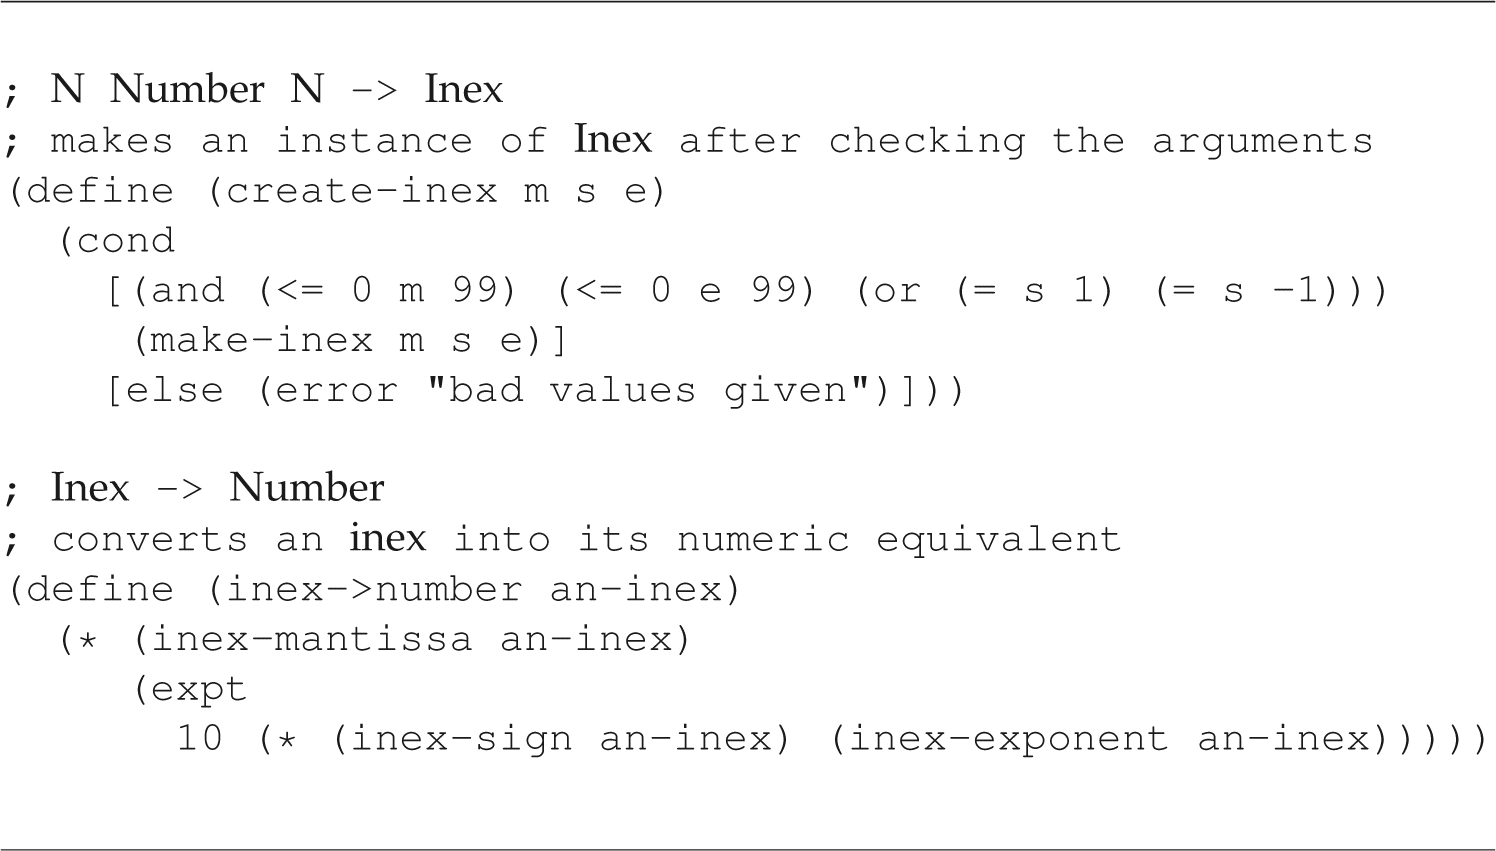
\includegraphics[width=0.85\textwidth]{images/00565.png}
  \caption{不精确数表示与转换函数 (Functions for inexact representations)}
  \label{fig:143}
\end{figure}

借助这一表示，我们可以明确界定可表示数字的范围：
\begin{lstlisting}[language=BSL]
(define MAX-POSITIVE (create-inex 99 1 99))
(define MIN-POSITIVE (create-inex 1 -1 99))
\end{lstlisting}

任何大于 \code{MAX-POSITIVE} 的正数，或者介于 0 与 \code{MIN-POSITIVE} 之间的微小正数，都\textbf{无法在该系统中找到等价表示}。此外，该表示在数轴中间存在巨大的“间隙”：例如 \code{(create-inex 12 1 2)}（即 1200）的下一个紧邻数是 \code{(create-inex 13 1 2)}（即 1300），介于 1200 与 1300 之间的任意数（例如 1240）只能被强行舍入近似到其中之一。这就是计算机科学中所说的\term{不精确数}（inexact numbers）。

\begin{exercise}{设计不精确数加法 inex+}{412}
设计函数 \code{inex+}。该函数实现两个 \code{Inex} 数字的加法运算。当两个输入的指数相同时，只需将尾数相加；当指数不同时，必须先对齐指数。若相加后的尾数超过 99，需进行进位与舍入处理。
\end{exercise}

\begin{exercise}{设计不精确数乘法 inex*}{413}
设计函数 \code{inex*}。该函数计算两个 \code{Inex} 数字的乘积：尾数相乘，指数相加，最后调整规格化并舍入。
\end{exercise}

\begin{exercise}{表示间隙与代数性质的丧失}{414}
由于存在舍入间隙，定长不精确数在数学上往往\textbf{不再满足加法结合律}或\textbf{乘法分配律}！试在你的 \code{Inex} 系统中找出三个数字 $a, b, c$，使得：
\[
(a + b) + c \neq a + (b + c)
\]
\end{exercise}

\intermezzosection{溢出与下溢 (Overflow and Underflow)}
\label{sec:int4_overflow_underflow}

当计算结果超出了系统所能表示的最大限度时，便发生了\term{算术溢出}（arithmetic overflow）。在 ISL+ 中，超出上限的浮点计算结果被标记为特殊值 \code{+inf.0}（表示正无穷大）或 \code{-inf.0}（负无穷大）。

反之，当一个非零计算结果太过于接近零，以至于其量级小于系统能表示的最小正数时，就发生了\term{算术下溢}（arithmetic underflow）。在 ISL+ 中，下溢被粗暴地截断近似为 \code{\#i0.0}。

\begin{exercise}{溢出界限探索}{415}
在 ISL+ 中，找出使得 \code{(expt 10.0 n)} 发生溢出并返回 \code{+inf.0} 的最小正整数 $n$。
\end{exercise}

\begin{exercise}{下溢界限探索}{416}
在 ISL+ 中，找出使得 \code{(expt 10.0 (- n))} 发生下溢并塌缩为 \code{\#i0.0} 的最小正整数 $n$。
\end{exercise}

\begin{exercise}{微指数幂运算精度对比}{417}
在完整 Racket 与 ISL+ 中分别求值表达式：
\begin{lstlisting}[language=BSL]
(expt 1.001 1e-12)
\end{lstlisting}
解释你在两个环境下观察到的输出差异。
\end{exercise}

\begin{exercise}{自定义幂函数 my-expt}{418}
不使用内置的 \code{expt}，针对整数指数设计递归幂函数 \code{my-expt}。在极大与极小测试用例上验证其行为。
\end{exercise}

\intermezzosection{灾难性抵消与求和次序 (Catastrophic Cancellation)}
\label{sec:int4_cancellation}

当一个极大的浮点数与一个极小的浮点数相加时，较小数的信息往往在指数对齐时被完全截断抹杀：
\begin{replbox}
> (+ 1e16 1.0 -1e16)
0.0
> (+ 1e16 (- 1e16) 1.0)
1.0
\end{replbox}
仅仅改变了运算的结合与求和次序，计算结果竟然相差了 $100\%$！

图~\ref{fig:144} 展示了一个著名的“双面简努斯”（Janus-faced）交错级数序列：正向累加与反向累加将得出天壤之别的荒谬结果。

\begin{figure}[htbp]
  \centering
  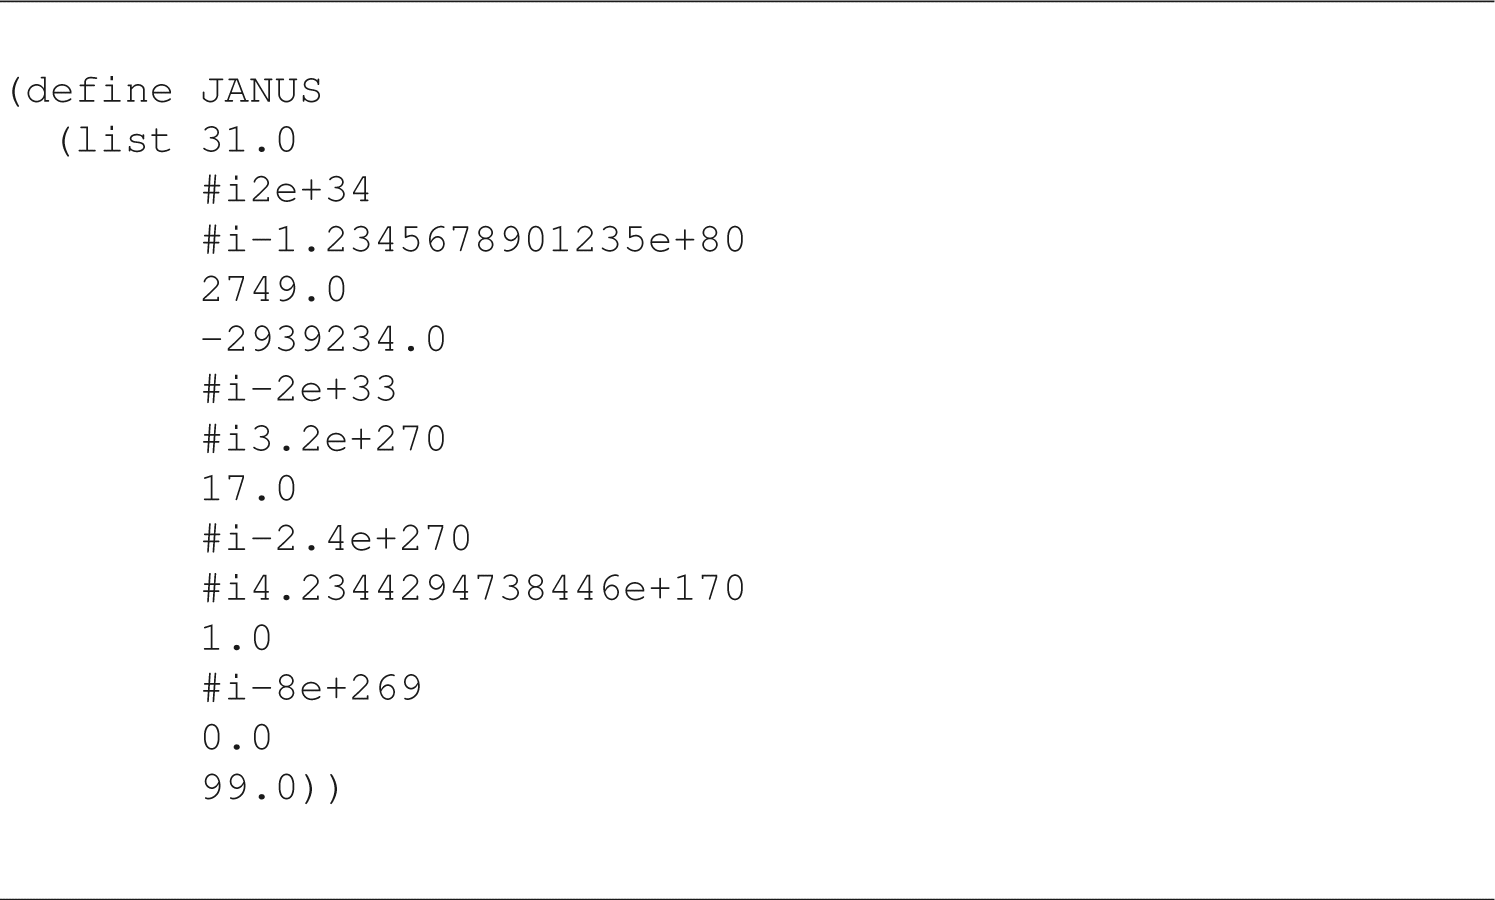
\includegraphics[width=0.85\textwidth]{images/00578.png}
  \caption{双面简努斯不精确数列 (A Janus-faced series of inexact numbers)}
  \label{fig:144}
\end{figure}

\begin{exercise}{求和次序对精度的剧烈影响}{419}
分别使用从左到右正向求和（\code{foldl}）与从右到左反向求和（\code{foldr}）计算图~\ref{fig:144} 中的数列之和。观察并分析两种不同求和方向所带来的致命精度偏差。
\end{exercise}

\begin{exercise}{数值震荡与混沌现象}{420}
考虑如下递归差分方程：
\begin{lstlisting}[language=BSL]
(define (oscillate n)
  (cond
    [(= n 0) 1.0]
    [else (- (* 2 (oscillate (sub1 n))) 1.0)]))
\end{lstlisting}
在纯数学上，$n=0$ 时为 1.0，随后每一项 $2(1.0) - 1.0 = 1.0$，序列应该恒等于 1.0。
然而在计算机浮点运算中，观察该函数随着 $n$ 的增大在图~\ref{fig:145} 中所呈现出的剧烈混沌震荡！
\end{exercise}

\begin{figure}[htbp]
  \centering
  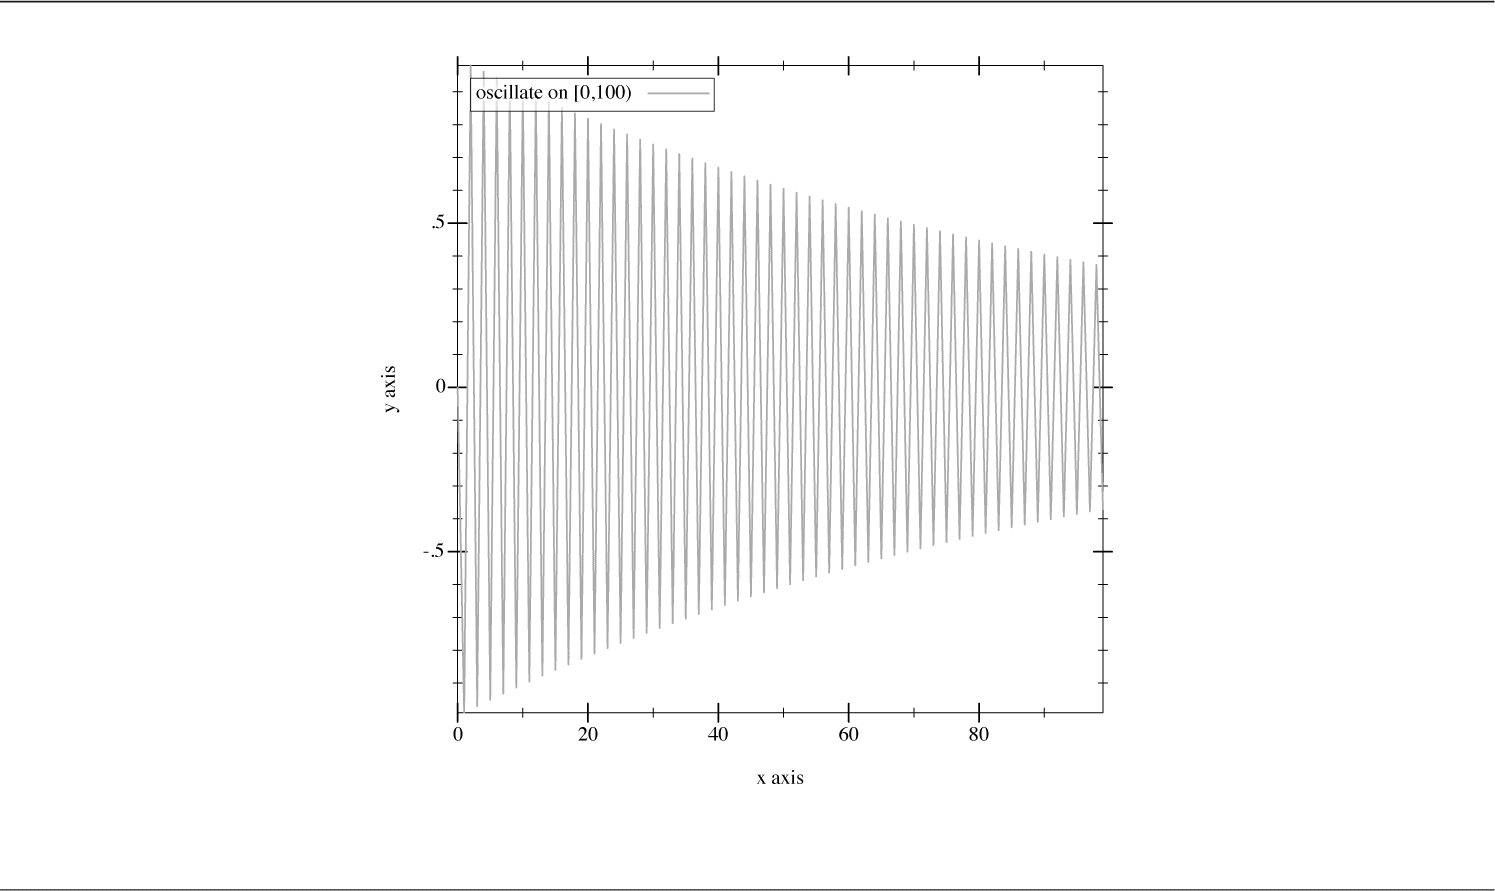
\includegraphics[width=0.85\textwidth]{images/00580.png}
  \caption{数值震荡与浮点混沌 (The graph of oscillate)}
  \label{fig:145}
\end{figure}

\begin{notebox}[结语：敬畏计算中的数字]
计算不仅是纯粹逻辑的演绎，更是物理机器对现实数学的有限逼近。作为优秀的程序设计者，在构建涉及工程、物理模拟与高频金融等涉及实数运算的系统时，必须始终对定长数的精度边界保持高度警惕与敬畏。
\end{notebox}


% ==================== 第五部分：生成式递归 ====================
\part{生成型递归 (Generative Recursion)}
% ==============================================================================
% 第 25 章：非结构驱动的递归 (Chapter 25: Recursion without Structure)
% ==============================================================================

\chapter{非结构驱动的递归}
\label{sec:ch25_nonstandard}

至此，你已经设计了大量采用\term{结构型递归（structural recursion）}的函数。设计这类函数时，你清楚地知道必须审视主输入的数据定义。如果该输入由自引用数据定义来描述，那么函数在形式上就会自然而在数据定义引用自身之处调用自身。

本章将介绍两个采用不同递归方式的示例程序。它们生动地展示了需要某种“顿悟”（eureka）的问题——从直观朴素的想法到精妙深刻的洞见各不相同。

\section{脱离数据结构的递归}
\label{sec:25_1}

设想你加入了 DrRacket 开发团队。团队正在研发一项协作分享服务，旨在支持程序员之间的协同工作。具体而言，DrRacket 的下一个版本将允许 ISL 程序员在多台计算机之间共享其 DrRacket 定义区的内容。每当一位程序员修改代码缓冲区时，更新后的 DrRacket 就会将定义区的内容广播给参与该分享会话的所有 DrRacket 实例。

\begin{notebox}[样例问题]
你的任务是设计 \code{bundle} 函数，负责将定义区的内容打包以便广播。DrRacket 将内容作为 \code{1String}（单字符字符串）列表交付。该函数的任务是将离散的“字符”打包成若干数据块（chunk），进而生成一个由给定长度（称为块大小 \code{chunk size}）的字符串组成的列表。
\end{notebox}

如你所见，问题叙述几乎直接给出了签名，并不需要专门定义新的数据：

\begin{lstlisting}[language=BSL]
; [List-of 1String] N -> [List-of String]
; 将 s 中的字符按长度 n 切块打包为字符串列表
(define (bundle s n)
  '())
\end{lstlisting}

目的说明重新组织了问题描述中的语句，并使用了虚拟函数头中的形参名称。

第三步是编写功能示例。给定一个 \code{1String} 列表：

\begin{lstlisting}[language=BSL]
(list "a" "b" "c" "d" "e" "f" "g" "h")
\end{lstlisting}

如果我们要求 \code{bundle} 将这个列表按两两成对打包（即 $n$ 为 2），那么预期结果应为如下列表：

\begin{lstlisting}[language=BSL]
(list "ab" "cd" "ef" "gh")
\end{lstlisting}

现在，如果 $n$ 改为 3，就会多出一个剩余的“字符”。由于问题描述并未指明剩余字符应当如何处置，我们可以设想至少两种合理的情形：

\begin{itemize}
  \item 函数生成 \code{(list "abc" "def" "g")}；即它将最后一个字符视作多余的零头保留在末尾。
  \item 或者，它生成 \code{(list "a" "bcd" "efg")}，将开头的字符单独打包为一个字符串。
\end{itemize}

\begin{notebox}[思考停步]
你能想出至少一种其他合理的处理方案吗？
\end{notebox}

为了简单起见，我们选择第一种方案作为预期结果，并写下相应的单元测试：

\begin{lstlisting}[language=BSL]
(check-expect (bundle (explode "abcdefg") 3)
              (list "abc" "def" "g"))
\end{lstlisting}

注意这里使用了 \code{explode}，它使得测试用例更加清晰易读。

示例与测试还必须涵盖数据定义边界处的情形。在此语境下，边界显然意味着传递给 \code{bundle} 的列表长度不足一个完整的块大小：

\begin{lstlisting}[language=BSL]
(check-expect (bundle '("a" "b") 3) (list "ab"))
\end{lstlisting}

这也意味着我们必须考虑当传入 \code{'()} 时 \code{bundle} 的行为。为简便起见，我们选择 \code{'()} 作为预期输出：

\begin{lstlisting}[language=BSL]
(check-expect (bundle '() 3) '())
\end{lstlisting}

另一种自然的选择是要求返回 \code{'("")}。你能看出其他可能吗？

设计模板这一步揭示了一个事实：传统的结构化方法在这里行不通。图~\ref{fig:bundle-templates} 展示了四种可能的模板。由于 \code{bundle} 的两个参数都是复杂数据，前两个模板将其中一个参数视为原子数据。这显然不对，因为函数必须同时拆解这两个参数。第三个模板假定两个参数以步调一致（lockstep）的方式同步递归，这看似接近——但 \code{bundle} 显然需要定期将块大小重置为其初始值。最后一个模板假定两个参数独立递归，这意味着在每个阶段都有四种继续的方式。这最后一种设计将参数解耦得过于彻底，因为列表与计数必须协同处理。简而言之，面对这一设计问题，传统的结构化模板显得无能为力。

\begin{figure}[htbp]
  \centering
  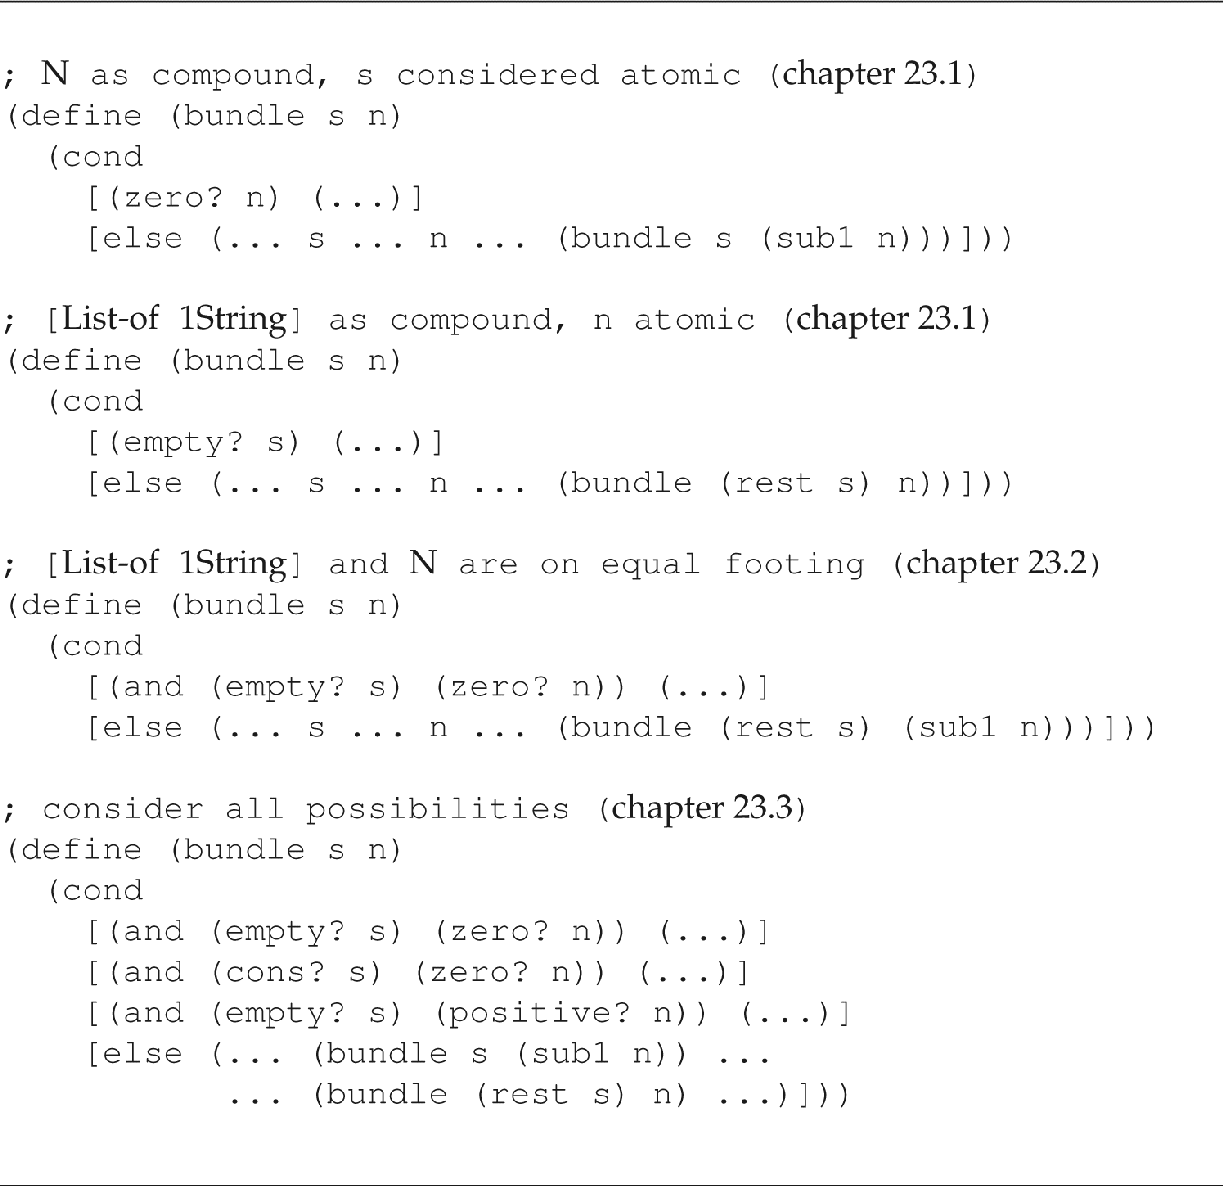
\includegraphics[width=0.85\textwidth]{images/00583.png}
  \caption{将字符串切块的四种无效模板}
  \label{fig:bundle-templates}
\end{figure}

图~\ref{fig:bundle-generative} 给出了 \code{bundle} 的完整定义。该定义使用了练习 395 中要求的 \code{drop} 和 \code{take} 函数；这些函数在标准库中也同样可用。为保持完整性，图中附带了它们的定义：\code{drop} 从列表头部至多丢弃 $n$ 个元素，而 \code{take} 则返回至多这么多个元素。借助这两个辅助函数，定义 \code{bundle} 就变得十分自然：

\begin{enumerate}
  \item 如果给定列表为 \code{'()}，结果如约返回 \code{'()}；
  \item 否则，\code{bundle} 使用 \code{take} 从 \code{s} 中取出前 $n$ 个 \code{1String}，并使用 \code{implode} 将其拼装成普通字符串；
  \item 接着，利用 \code{drop} 剔除前 $n$ 个元素，在缩短后的子列表上进行递归调用；
  \item 最后，使用 \code{cons} 将第 2 步得到的字符串与第 3 步得到的字符串列表组合起来，生成针对完整列表的最终结果。
\end{enumerate}

\begin{figure}[htbp]
  \centering
  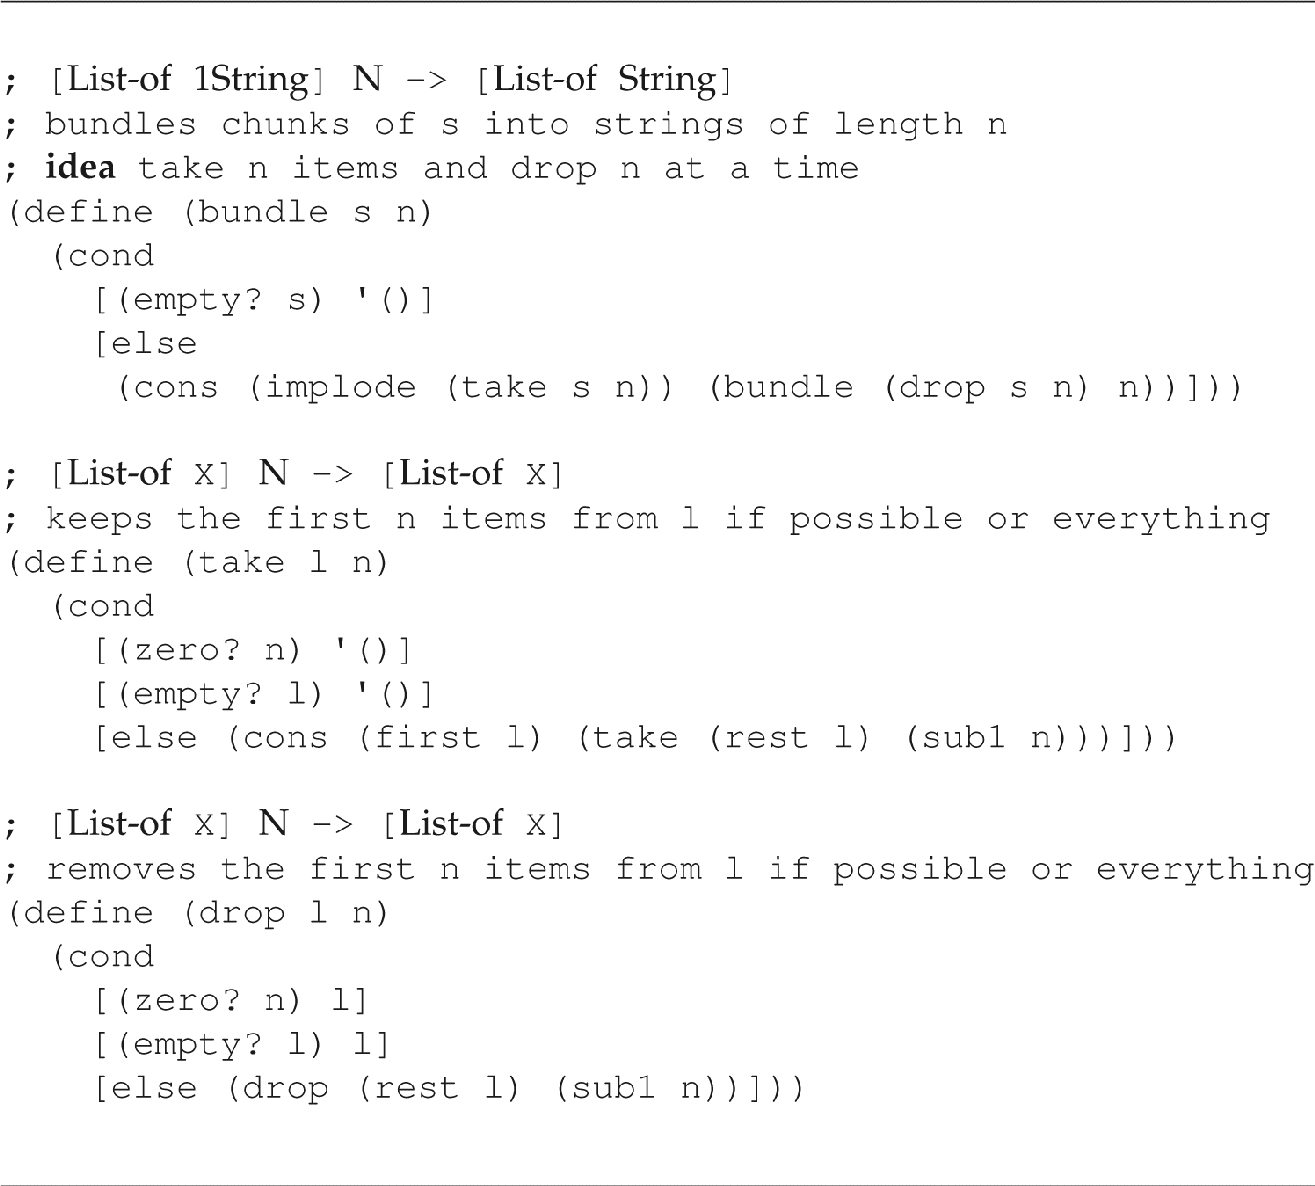
\includegraphics[width=0.85\textwidth]{images/00584.png}
  \caption{生成型递归：\code{bundle} 及其辅助函数的完整定义}
  \label{fig:bundle-generative}
\end{figure}

上述第 3 项凸显了 \code{bundle} 与本书前四部分中所有函数的根本差异。由于 \code{List-of} 的数据定义是通过在已有列表上 \code{cons} 一个元素来构造新列表的，因此前四部分中的所有函数都使用 \code{first} 和 \code{rest} 来解构非空列表。相比之下，\code{bundle} 使用了 \code{drop}，它一次性丢弃的不仅是一个元素，而是整整 $n$ 个元素。

尽管 \code{bundle} 的定义很不寻常，但其底层思想非常直观，与我们目前见过的函数也没有太大偏离。事实上，当块大小 $n$ 等于 1 时，\code{bundle} 就退化为标准的结构型递归定义。此外，\code{drop} 保证生成给定列表的一个组成部分，而不是某种任意打乱重排的版本。而这种思路正是下一节所要探讨的核心。

\begin{exercise}{调用 bundle 与边界情况}{421}\label{ex:421}
表达式 \code{(bundle '("a" "b" "c") 0)} 是对 \code{bundle} 函数的合法调用吗？它会产生什么结果？为什么？
\end{exercise}

\begin{exercise}{基于列表切块定义 bundle}{422}\label{ex:422}
定义函数 \code{list->chunks}。该函数接收任意数据的列表 \code{l} 以及自然数 \code{n}。函数的结果是大小为 \code{n} 的列表块的列表。每个块代表 \code{l} 中项的一个连续子序列。

请使用 \code{list->chunks} 通过函数组合来定义 \code{bundle}。
\end{exercise}

\begin{exercise}{基于字符串切片的 partition 函数}{423}\label{ex:423}
定义函数 \code{partition}。它接收一个字符串 \code{s} 和自然数 \code{n}。函数生成一个由长度为 \code{n} 的字符串切块组成的列表。

对于非空字符串 \code{s} 与正自然数 \code{n}，以下等式应当成立：
\begin{lstlisting}[language=BSL]
(equal? (partition s n) (bundle (explode s) n))
\end{lstlisting}
但请不要直接将该等式作为 \code{partition} 的定义，而应使用 \code{substring}。

\textbf{提示}：让 \code{partition} 对空字符串产生其自然的结果。对于 $n = 0$ 的情况，请参考练习~\ref{ex:421}。

\textbf{注}：相比 \code{bundle}，\code{partition} 函数更贴近协同 DrRacket 环境的实际需求。
\end{exercise}

\section{忽略结构的递归}
\label{sec:25_2}

回顾第 11 章中的 \code{sort>} 函数，它接收一个数字列表并按某种顺序（通常是升序或降序）重新排列。它的工作机制是将第一个数字插入到剩余列表排序后所得列表的合适位置。换言之，它是一个结构型递归函数，对自然递归的结果进行后处理。

霍尔（C. A. R. Hoare）的\term{快速排序算法（quick-sort algorithm）}则以一种截然不同的方式对列表进行排序，并成为了\term{生成型递归（generative recursion）}的经典范例。其底层的生成步骤采用了久经考验的\term{分治策略（divide-and-conquer strategy）}：将问题的非平凡实例划分为两个规模更小且相关的子问题；求解这两个子问题；然后将子问题的解合并为原问题的解。就快速排序算法而言，其中间目标是将数字列表划分为两个子列表：
\begin{itemize}
  \item 一个包含所有严格小于第一个数字的元素；
  \item 另一个包含所有严格大于第一个数字的元素。
\end{itemize}
随后，使用快速排序算法对这两个较小的子列表进行递归排序。一旦两个子列表完成排序，就将它们组合起来，并将第一个元素放置在中间。鉴于其特殊的枢纽角色，列表中的第一个元素被称为\term{基准元（pivot item，或枢轴元）}。

为了深入理解快速排序的工作原理，我们通过一个具体例子来演练对 \code{(list 11 8 14 7)} 进行快速排序的过程。图~\ref{fig:quicksort-diagram} 以图形化方式直观展示了这一过程。整张图由上半部分的“划分阶段”（divide phase）与下半部分的“合并解决阶段”（conquer phase）组成。

\begin{figure}[htbp]
  \centering
  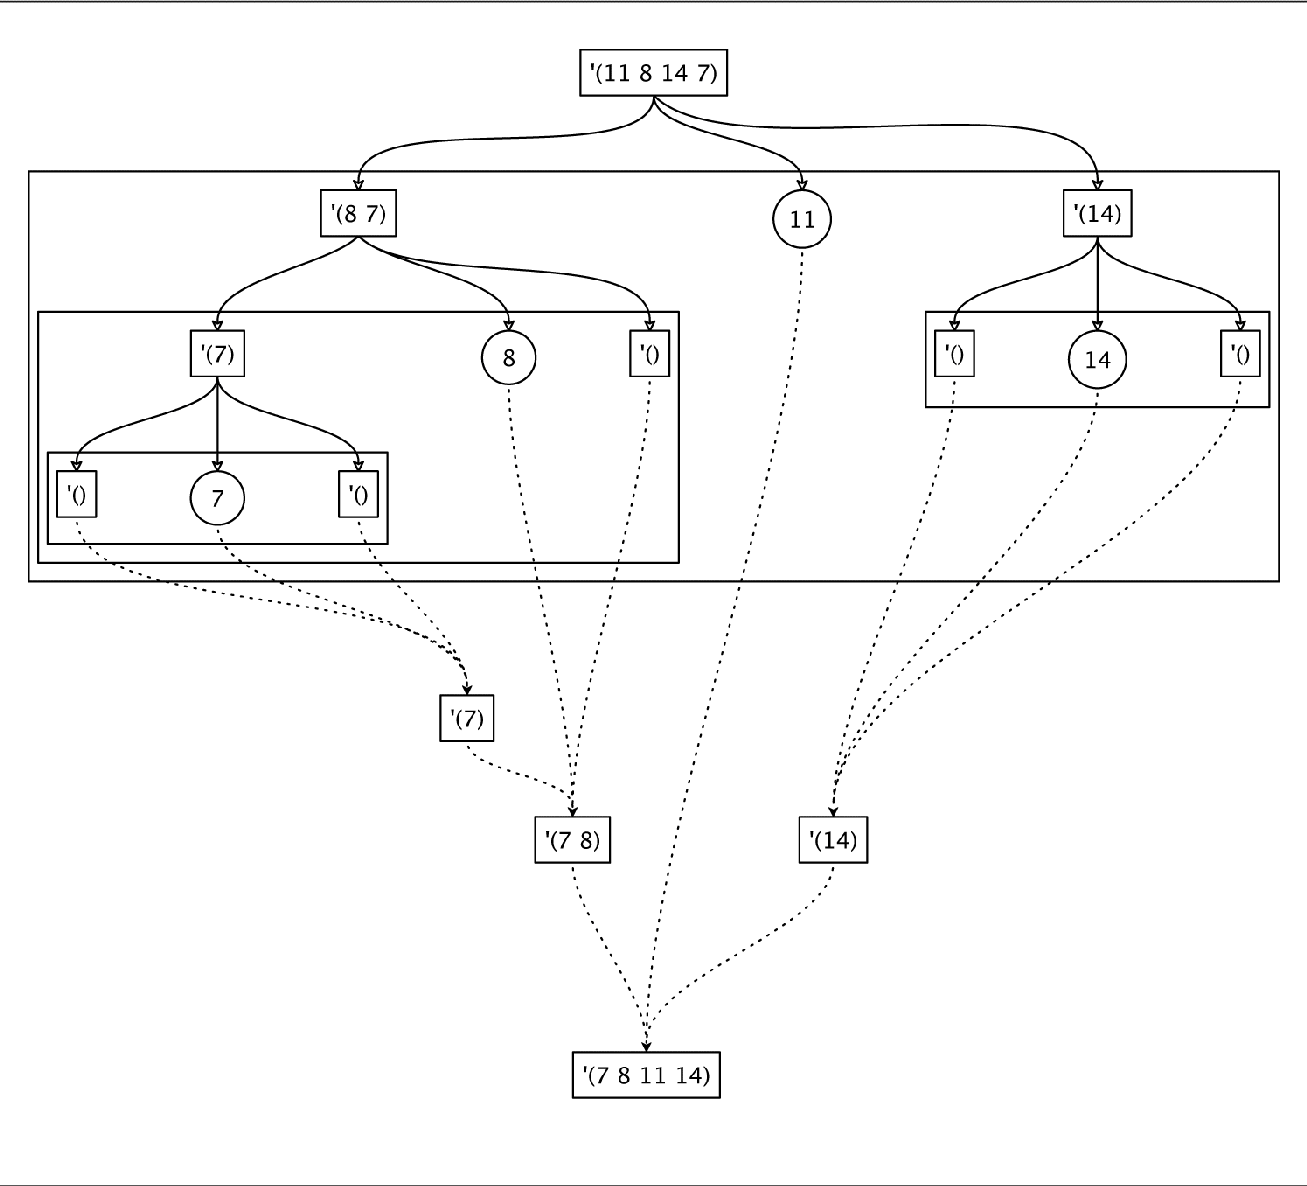
\includegraphics[width=0.85\textwidth]{images/00585.png}
  \caption{快速排序算法的图解过程}
  \label{fig:quicksort-diagram}
\end{figure}

划分阶段由带框列表与实线箭头表示。每个带框列表引出三条箭头，指向一个包含三部分的框：中间是带圆圈的基准元，其左侧是比基准元小的数字列表，其右侧是比基准元大的数字列表。每一步都至少隔离出一个数字作为基准元，这意味着左右两个相邻列表的长度都严格小于给定的原列表。因此，整个划分过程必然会终止。

考虑输入为 \code{(list 11 8 14 7)} 的第一步：基准元是 \code{11}。将列表划分为小于和大于 \code{11} 的元素，分别得到 \code{(list 8 7)} 和 \code{(list 14)}。划分阶段的其余步骤以类似方式工作。当所有数字都被隔离为基准元时，划分阶段结束。此时，只要从左向右读取所有的基准元，就能直接读出最终的排序结果。

合并解决阶段由虚线箭头与带框列表表示。三条箭头汇入每个结果框：中间一条来自基准元，左侧来自较小数字排序后的结果，右侧来自较大数字排序后的结果。每一步都将至少一个数字（即基准元）加入结果列表，这意味着列表朝向图的底部不断增长。底部的框就是顶部给定列表的有序排列。

观察最左上角的合并步骤：它将基准元 \code{7} 与两个空列表合并，得到 \code{'(7)}。再下一级对应于隔离出 \code{8} 的划分步骤，从而生成 \code{'(7 8)}。合并解决阶段的每一层级都镜像映射了划分阶段的对应层级。归根结底，整个过程是递归的。

\begin{exercise}{绘制快速排序追踪图}{424}\label{ex:424}
针对列表 \code{(list 11 9 2 18 12 14 4 1)}，绘制一张类似于图~\ref{fig:quicksort-diagram} 的快速排序执行图。
\end{exercise}

既然我们已经充分理解了快速排序的思想，就可以将其翻译为 ISL+ 代码。显而易见，\code{quick-sort<} 区分两种情况：如果输入是 \code{'()}，由于空列表本身已经有序，直接产生 \code{'()}；否则，执行生成型递归。这种情形划分提示了如下 \code{cond} 表达式：

\begin{lstlisting}[language=BSL]
; [List-of Number] -> [List-of Number]
; 生成 alon 的升序排列版本
; 假设所有数字互不相同
(define (quick-sort< alon)
  (cond
    [(empty? alon) '()]
    [else (... (first alon) ... (rest alon) ...)]))
\end{lstlisting}

第一种情况的结果不言自明。对于第二种情况，当 \code{quick-sort<} 的输入为非空列表时，算法利用首个元素将列表的其余部分划分为两个子列表：一个包含所有小于基准元的项，另一个包含所有大于基准元的项。

由于剩余列表的长度未知，我们将列表划分的任务委托给两个辅助函数：\code{smallers} 和 \code{largers}。它们遍历列表，分别过滤出小于和大于基准元的元素。因此，每个辅助函数都接收两个参数：一个数字列表和一个数字。设计这两个函数是一次标准结构型递归的练习。你可以尝试独立编写，或者阅读图~\ref{fig:quicksort-full} 中给出的定义。

\begin{figure}[htbp]
  \centering
  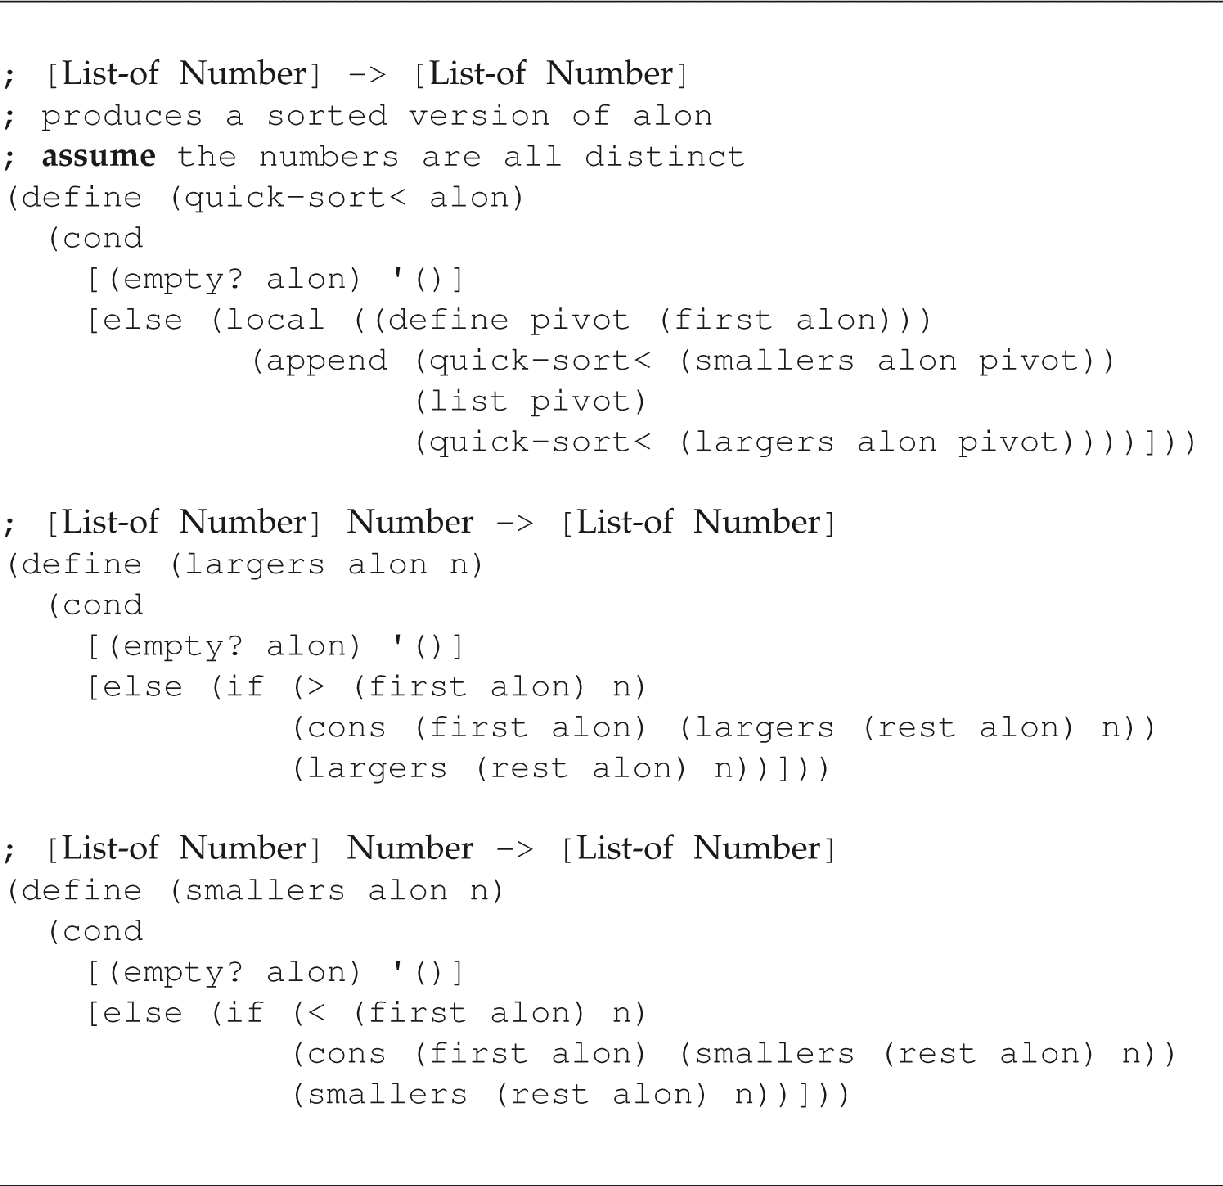
\includegraphics[width=0.85\textwidth]{images/00587.png}
  \caption{快速排序算法及辅助函数}
  \label{fig:quicksort-full}
\end{figure}

这两个子列表分别使用 \code{quick-sort<} 进行独立排序，这构成了递归调用，具体表现为如下两个表达式：
\begin{enumerate}
  \item \code{(quick-sort< (smallers alon pivot))}：对所有小于基准元的元素进行排序；
  \item \code{(quick-sort< (largers alon pivot))}：对所有大于基准元的元素进行排序。
\end{enumerate}

一旦 \code{quick-sort<} 获得了两个子列表排序后的版本，就必须按恰当的顺序将两部分与基准元拼接起来：首先是所有小于 \code{pivot} 的项，接着是 \code{pivot}，最后是所有大于它的项。由于第一部分和最后一部分已经排好序，\code{quick-sort<} 只需简单使用 \code{append}：

\begin{lstlisting}[language=BSL]
(append (quick-sort< (smallers (rest alon) pivot))
        (list pivot)
        (quick-sort< (largers (rest alon) pivot)))
\end{lstlisting}

图~\ref{fig:quicksort-full} 包含了完整的程序；在继续阅读之前请仔细研读它。

有了具体的函数定义后，我们可以手工推导前面示例的求值过程：

\begin{lstlisting}[language=BSL]
  (quick-sort< (list 11 8 14 7))
== (append (quick-sort< (list 8 7))
           (list 11)
           (quick-sort< (list 14)))
== (append (append (quick-sort< (list 7))
                   (list 8)
                   (quick-sort< '()))
           (list 11)
           (quick-sort< (list 14)))
== (append (append (append (quick-sort< '())
                           (list 7)
                           (quick-sort< '()))
                   (list 8)
                   '())
           (list 11)
           (quick-sort< (list 14)))
== ...
\end{lstlisting}

这一推演展示了排序过程的核心步骤，即划分步骤、递归排序步骤以及三部分的拼接。从该推演中，很容易看出 \code{quick-sort<} 是如何实现图~\ref{fig:quicksort-diagram} 中所示过程的。

图~\ref{fig:quicksort-diagram} 与手动计算都清晰表明：\code{quick-sort<} 完全忽略了给定列表的既有结构。第一次递归作用于原始列表中相隔甚远的两个数字，而第二次递归作用于列表的第三个元素。这些递归调用绝非随机产生，但它们显然不再依赖于数据定义的自然结构。

将 \code{quick-sort<} 的组织结构与第 11 章中的 \code{sort>} 函数进行对比：后者的设计严格遵循结构化设计配方，生成逐个处理列表项的程序。而通过对列表进行划分，\code{quick-sort<} 能够极大地加快列表排序的过程——其代价则是不再使用简单的 \code{first} 与 \code{rest} 遍历。

\begin{exercise}{为 smallers 与 largers 编写目的说明}{425}\label{ex:425}
为图~\ref{fig:quicksort-full} 中的 \code{smallers} 与 \code{largers} 辅助函数清晰阐述其目的说明。
\end{exercise}

\begin{exercise}{单元素列表的平凡情形优化}{426}\label{ex:426}
完成上述手工推导过程。仔细检查求值步骤会揭示 \code{quick-sort<} 的一个额外的平凡情形（trivial case）：每当 \code{quick-sort<} 接收只有一个元素的列表时，它都可以直接原样返回该列表。毕竟，只有一个元素的列表本身必然是有序的。

请修改 \code{quick-sort<} 以利用这一观察结果。重新推导上述示例。修改后的算法节省了多少个求值步骤？
\end{exercise}

\begin{exercise}{结合插入排序的阈值混合排序}{427}\label{ex:427}
虽然在多数情况下 \code{quick-sort<} 能迅速缩小问题规模，但对于极小规模的问题，它的开销却相对过大。因此，工程实践中常使用 \code{quick-sort<} 来减小问题规模，当列表缩减到足够小时则切换到另一种排序函数。

请开发一个 \code{quick-sort<} 的改进版本：当输入列表的长度低于某个阈值时，切换使用 \code{sort<}（即第 11.3 节中 \code{sort>} 的升序适配版本）。
\end{exercise}

\begin{exercise}{处理包含重复数字的列表}{428}\label{ex:428}
如果传给 \code{quick-sort<} 的输入列表中包含多个相同的数字，算法返回的列表长度将严格小于输入的长度。为什么会出现这种现象？请修正该问题，使得输出列表与输入列表长度相同且保留所有重复项。
\end{exercise}

\begin{exercise}{使用 filter 定义 smallers 与 largers}{429}\label{ex:429}
使用抽象函数 \code{filter} 重新定义 \code{smallers} 与 \code{largers}。
\end{exercise}

\begin{exercise}{单一比较算子与抽象快速排序}{430}\label{ex:430}
开发 \code{quick-sort<} 的一个变体，它只使用单一比较函数（例如 \code{<}）。其划分步骤将给定的列表 \code{alon} 划分为一个包含所有小于基准元的元素列表，以及另一个包含所有不小于基准元的元素列表。

使用 \code{local} 将程序封装为一个单一函数。随后对该函数进行抽象，使其接收一个列表和一个通用比较谓词作为参数。
\end{exercise}

% ==============================================================================
% 第 26 章：设计算法 (Chapter 26: Designing Algorithms)
% ==============================================================================

\chapter{设计算法}
\label{sec:ch26_algorithms}

正如本部分的引言所指出的，设计生成型递归函数比结构化设计更加因题而异（ad hoc）。第 25 章表明，两个生成型递归函数在处理机制上可能存在天壤之别：\code{bundle} 和 \code{quick-sort<} 虽然都处理列表，但前者至少维持了给定列表中的元素先后次序，而后者则随心所欲地重新排列列表元素。这就带来了一个深刻的疑问：单一的设计配方能否指导如此大相径庭的函数设计？

本节首先展示如何将设计配方的各个维度调整适配于生成型递归。第二节聚焦于一个全新现象：算法可能对于某些输入根本无法产生答案。因此，程序员必须分析自己的程序，并用终止性（termination）说明来补充设计文档。后续各节将深入对比结构型递归与生成型递归的异同与选择策略。

\section{调整设计配方}
\label{sec:26_1}

让我们结合前一章的示例，重新审视结构化设计配方的六个通用步骤：

\begin{itemize}
  \item \textbf{问题分析与数据表示}：与以往一样，我们必须在选定的编程语言中将问题信息表示为数据。对问题数据表示的选择直接影响我们对计算过程的思考，因此需要预先规划；或者做好回溯并探索不同数据表示的准备。无论如何，我们都必须分析问题信息并明确定义数据集合。
  \item \textbf{签名、函数头与目的说明}：我们同样需要签名、函数头和目的说明。由于生成步骤与输入数据的结构定义不再直接绑定，目的说明不能仅仅停留在函数\term{计算什么}（what），还必须解释函数\term{如何计算}（how）其结果。
  \item \textbf{功能示例}：通过功能示例来阐释“如何计算”极为有益，就像前一章解释 \code{bundle} 和 \code{quick-sort<} 那样。在结构化世界中，功能示例只需指明特定输入应产生何种输出；而在生成型递归中，示例的核心目的在于解释计算过程背后的\term{生成思想}。
  
  对于 \code{bundle}，示例说明了函数在一般情况以及特定边界情形下的行为。对于 \code{quick-sort<}，图~\ref{fig:quicksort-diagram} 中的示例直观展示了函数如何依据基准元划分给定列表。将此类推演示例加入目的说明中，我们作为设计者能更清晰地理解预期的计算过程，并能将这种理解准确传递给未来的代码读者。
  \item \textbf{函数模板}：我们的讨论催生了一个算法的通用设计模板。粗略地说，算法的设计将问题区分为两类：\term{平凡可解的问题}（trivially solvable problems）与\term{非平凡问题}。若给定问题是平凡可解的，算法直接产生对应的解（例如对空列表或单元素列表进行排序属于平凡情形）。包含多个元素的列表则是非平凡问题。对于非平凡问题，算法通常会生成一个或多个与原问题同类的新问题，递归求解这些子问题，最后将子问题的解合并为原问题的完整解。
\end{itemize}

\begin{notebox}[关于“平凡”的术语说明]
在本部分中，“平凡”（trivial）是一个严格的计算机科学术语，指可以直接求解而无需进一步生成子问题的情形（即递归基）。
\end{notebox}

根据这一定性描述，所有算法大致都具有如下代码组织结构：

\begin{lstlisting}[language=BSL]
(define (generative-recursive-fun problem)
  (cond
    [(trivially-solvable? problem)
     (determine-solution problem)]
    [else
     (combine-solutions
       ... problem ...
       (generative-recursive-fun
         (generate-problem-1 problem))
       ...
       (generative-recursive-fun
         (generate-problem-n problem)))]))
\end{lstlisting}

有时候合并子问题的解需要用到原问题的某些数据（例如快速排序需要插入原始的基准元），因此原问题的数据也会按需传递给 \code{combine-solutions}。

这一模板只是一幅富有启发性的设计蓝图，而非僵化的死板框架。模板中的各个组成部分提醒我们必须认真思考以下四个核心问题：

\begin{enumerate}
  \item \textbf{何为平凡可解的问题？}
  \item \textbf{平凡问题如何直接求解？}
  \item \textbf{算法如何生成比原问题更容易求解的新问题？生成的是一个还是多个新问题？}
  \item \textbf{原问题的解是否与新问题的解相同？还是说我们需要合并子问题的解来构造原问题的解？若是后者，是否需要借用原问题的原始数据？}
\end{enumerate}

为了将算法定义为具体函数，我们必须基于选定的数据表示，用代码和辅助函数来准确回答上述四个问题。

在这一阶段，第 9 章介绍的表格推导法能再次大显身手。以快速排序为例，其核心是将列表划分为更小与更大的两组数并分别排序。图~\ref{fig:combine-table} 展示了若干简单数值示例在非平凡情形下的拆解与合并过程。从这些示例中，很容易猜出第 4 个问题的答案：将较小数排序后的列表、基准元以及较大数排序后的列表拼接在一起，这一思路直接映射为代码中的 \code{append}。

\begin{figure}[htbp]
  \centering
  \begin{tabular}{|l|c|l|l|l|}
    \hline
    \textbf{alon} & \textbf{pivot} & \textbf{排序后的较小元素} & \textbf{排序后的较大元素} & \textbf{预期结果} \\
    \hline
    \code{'(2 3 1 4)} & \code{2} & \code{'(1)} & \code{'(3 4)} & \code{'(1 2 3 4)} \\
    \code{'(2 0 1 4)} & \code{2} & \code{'(0 1)} & \code{'(4)} & \code{'(0 1 2 4)} \\
    \code{'(3 0 1 4)} & \code{3} & \code{'(0 1)} & \code{'(4)} & \code{'(0 1 3 4)} \\
    \hline
  \end{tabular}
  \caption{用于猜测解的组合方式的表格推导法}
  \label{fig:combine-table}
\end{figure}

当函数主体完成后，最后一步是进行充分测试以排查并消除缺陷。

\begin{exercise}{回答四个核心设计问题}{431}\label{ex:431}
针对 \code{bundle} 问题回答上述四个核心问题；针对 \code{quick-sort<} 问题回答前三个问题。在每种情况下各需要多少个 \code{generate-problem} 实例？
\end{exercise}

\begin{exercise}{重构与论证 food-create}{432}\label{ex:432}
练习 219 介绍了 \code{food-create} 函数，它接收一个 \code{Posn} 并生成一个随机选择的、保证与给定点不同的新 \code{Posn}。请先使用 \code{local} 将其重构成单一函数定义，然后依照上述四个问题论证 \code{food-create} 的算法设计。
\end{exercise}

\section{终止性分析}
\label{sec:26_2}

生成型递归为计算引入了一个截然不同的全新维度：\term{非终止性（non-termination）}。对于某些特定输入，诸如 \code{bundle} 这样的函数可能永远无法产生值，也不会报错中断。练习~\ref{ex:421} 询问 \code{(bundle '("a" "b" "c") 0)} 的计算结果，以下求值推导展示了它为何没有结果：

\begin{lstlisting}[language=BSL]
  (bundle '("a" "b" "c") 0)
== (cons (implode (take '("a" "b" "c") 0))
         (bundle (drop '("a" "b" "c") 0) 0))
== (cons (implode '())
         (bundle (drop '("a" "b" "c") 0) 0))
== (cons "" (bundle '("a" "b" "c") 0))
\end{lstlisting}

推导表明，为了求出 \code{(bundle '("a" "b" "c") 0)} 的值，必须先获得\textbf{完全相同}表达式的求值结果！在 ISL+ 环境中，这意味着求值永远无法结束。计算机科学家称：当第二个参数为 0 时 \code{bundle} \term{不会停机（does not terminate）}；也可以说该函数\term{死循环（loops）}，或者计算陷入了\term{无限循环（infinite loop）}。

将这一现象与前四部分的设计进行对比：依据结构化配方设计的每一个函数，对于每一个合法输入，要么产生答案，要么显式抛出错误信号。这是因为结构化配方严格要求每一次自然递归都只消耗输入的直接子结构，而不是输入本身。由于数据是按层次递归构造的，输入在每个阶段都会缩减，最终必然到达原子数据（基准情形），递归随即终止。

这解释了生成型递归函数为何可能发散（diverge）。根据生成型递归的设计配方，算法生成新子问题是不受任何结构限制的。如果配方强制要求新问题必须在某种度量下严格“小于”原问题，算法自然能够保证终止。然而，施加这种武断的限制在设计阶段往往过于苛刻。

因此，在生成型递归的设计配方中，我们保留前六个步骤，并补充了至关重要的第七个步骤：\term{终止性论证（termination argument）}。

\begin{recipebox}{生成型递归设计配方}
\textbf{步骤 1：问题分析与数据表示} \\
确定问题的数据表示；定义数据集合。

\textbf{步骤 2：签名、函数头与目的说明} \\
给出函数签名；目的说明不仅阐述函数\textbf{计算什么}，还需用一句话说明它\textbf{如何计算}。

\textbf{步骤 3：功能示例} \\
给出测试用例；通过具体实例展示算法“如何”一步步生成子问题并合并解。

\textbf{步骤 4：设计模板} \\
区分平凡情形与非平凡情形；划分 \code{cond} 分支结构。

\textbf{步骤 5：函数定义} \\
明确平凡可解的条件与解法；确定如何生成新子问题以及如何合并子问题的解。

\textbf{步骤 6：测试} \\
运行测试用例，发现并纠正错误。

\textbf{步骤 7：终止性论证} \\
论证程序为何能终止，形式为以下二者之一：
\begin{enumerate}
  \item \textbf{规模缩减论证}：说明为何每次递归调用的子问题规模都严格小于当前输入规模；
  \item \textbf{非停机异常说明}：举例说明在何种数据情形下函数可能陷入死循环。
\end{enumerate}
\end{recipebox}

终止性论证通常采取两种形式之一。第一种形式是论证为什么每次递归调用处理的问题规模都严格小于当前问题。通常这种论证很直观，但在极少数复杂情况下可能需要借助数学定理证明。第二种形式则是举例说明函数在哪些输入下无法停机，并清晰界定导致死循环的数据类别。

我们用具体示例来说明这两种终止性论证。对于 \code{bundle} 函数，在目的说明中向读者警示块大小为 0 的情况即可：

\begin{lstlisting}[language=BSL]
; [List-of 1String] N -> [List-of String]
; 将 s 中的字符序列按长度 n 打包成字符串
; 停机性：除非 s 为 '()，否则 (bundle s 0) 将陷入死循环
(define (bundle s n) ...)
\end{lstlisting}

对于 \code{quick-sort<}，关键观察在于每次递归调用接收的列表长度都严格小于输入列表 \code{alon}：

\begin{lstlisting}[language=BSL]
; [List-of Number] -> [List-of Number]
; 生成 alon 的升序排序列表
; 停机性：quick-sort< 的两次递归调用所接收的列表均剔除了基准元 pivot，
; 因而列表长度均严格小于 alon
(define (quick-sort< alon) ...)
\end{lstlisting}

\begin{exercise}{保证终止的 checked-bundle}{433}\label{ex:433}
开发一个校验版本 \code{checked-bundle}，保证对所有输入都能停机。在原版本会导致死循环的输入情形下，该函数应当显式抛出友好的错误提示。
\end{exercise}

\begin{exercise}{错误的 smallers 导致死循环}{434}\label{ex:434}
考虑如下 \code{smallers} 的错误定义（快速排序的两个问题生成器之一）：

\begin{lstlisting}[language=BSL]
(define (smallers alon n)
  (cond
    [(empty? alon) '()]
    [else (if (<= (first alon) n)
              (cons (first alon) (smallers (rest alon) n))
              (smallers (rest alon) n))]))
\end{lstlisting}

当在第 25.2 节的 \code{quick-sort<} 中使用该版本时，会发生什么严重错误？为什么？
\end{exercise}

\begin{exercise}{加固快速排序的停机性}{435}\label{ex:435}
在完成练习 428 或练习 430 时，你可能会写出死循环的解法。同样，练习~\ref{ex:434} 揭示了快速排序的停机性论据是多么脆弱：整个论证完全仰赖于 \code{smallers} 和 \code{largers} 生成的列表均不包含 \code{pivot}，从而保证列表长度严格缩减。

基于这一分析，请修改 \code{quick-sort<} 的内部定义，使得传递给 \code{smallers} 和 \code{largers} 的列表本身就事先移除了首元素（即传入 \code{(rest alon)}），从而在结构上确保子问题必定缩短。
\end{exercise}

\begin{exercise}{论证 food-create 的停机性}{436}\label{ex:436}
为练习~\ref{ex:432} 中的 \code{food-create} 函数撰写完整的终止性论证。
\end{exercise}

\section{结构型递归与生成型递归的对比}
\label{sec:26_3}

算法的通用模板极其宽泛，以至于它实际上涵盖了所有的结构型递归函数。考察图~\ref{fig:gen-to-struct} 的左侧：该模板针对一个平凡分支和一个生成步骤进行了特化。如果我们将其中的 \code{trivial?} 替换为 \code{empty?}，并将 \code{generate} 替换为 \code{rest}，就会立即得到右侧的标准列表处理模板！

\begin{figure}[htbp]
  \centering
  \begin{minipage}{0.48\textwidth}
\begin{lstlisting}[language=BSL]
(define (general P)
  (cond
    [(trivial? P) (solve P)]
    [else
     (combine-solutions
       P
       (general
         (generate P)))]))
\end{lstlisting}
  \end{minipage}
  \hfill
  \begin{minipage}{0.48\textwidth}
\begin{lstlisting}[language=BSL]
(define (special P)
  (cond
    [(empty? P) (solve P)]
    [else
     (combine-solutions
       P
       (special (rest P)))]))
\end{lstlisting}
  \end{minipage}
  \caption{从生成型递归到结构型递归的特化}
  \label{fig:gen-to-struct}
\end{figure}

\begin{exercise}{特化模板的求解与合并}{437}\label{ex:437}
为上述 \code{special} 模板分别定义 \code{solve} 与 \code{combine-solutions}，使得：
\begin{enumerate}
  \item \code{special} 计算输入列表的长度；
  \item \code{special} 对给定数字列表中的每个数取相反数；
  \item \code{special} 将给定字符串列表中的每个字符串转换为大写。
\end{enumerate}
从这些练习中你能得出什么结论？
\end{exercise}

此时你可能会思索：结构型递归设计与生成型递归设计之间是否存在本质区别？我们的回答是：“视情况而定”。从纯形式角度看，所有结构型递归函数都可以被视为生成型递归的特例。然而，这种“万物皆同”的泛化态度对于理解程序设计过程毫无益处。它混淆了两种需要截然不同的思维方式、且具有完全不同后果的设计方法：
\begin{itemize}
  \item \textbf{结构型递归}完全依赖于系统化的\textbf{数据分析}，只要跟随数据定义的节奏就能自然写出模板，并且天然保证终止；
  \item \textbf{生成型递归}则依赖于对问题求解机制本身的深刻洞见，通常蕴含着数学算法层面的“灵感顿悟”（eureka），而且必须显式提供终止性论证。
\end{itemize}
将这两种截然不同的设计途径混为一谈是有害的。

\section{方案抉择}
\label{sec:26_4}

当你在程序中使用一个对数字列表进行排序的函数 $f$ 时，从外部观察，你根本无法分辨 $f$ 究竟是 \code{sort<}（插入排序）还是 \code{quick-sort<}（快速排序）。这两个函数在可观测行为上是完全等价的（observably equivalent）。这就带来了一个现实问题：编程语言究竟应当提供哪一个？更广泛地说，当既可以用结构型递归又可以用生成型递归来解决一个问题时，我们该如何抉择？

为了阐明这种抉择的深远影响，我们探讨数学中的一个经典范例：寻找两个正自然数的\term{最大公约数（greatest common divisor, gcd）}。所有正整数都有公约数 1；在某些情况下（如 2 与 3），1 也是它们唯一的公约数。而 6 与 25 则分别拥有多个约数：
\begin{itemize}
  \item 6 能被 1, 2, 3, 6 整除；
  \item 25 能被 1, 5, 25 整除。
\end{itemize}
它们的最大公约数依然是 1。相比之下，18 和 24 拥有多个公约数，它们的最大公约数是 6：
\begin{itemize}
  \item 18 能被 1, 2, 3, 6, 9, 18 整除；
  \item 24 能被 1, 2, 3, 4, 6, 8, 12, 24 整除。
\end{itemize}

完成设计配方的前三步十分直接：

\begin{lstlisting}[language=BSL]
; N[>= 1] N[>= 1] -> N
; 计算 n 和 m 的最大公约数
(check-expect (gcd 6 25) 1)
(check-expect (gcd 18 24) 6)
(define (gcd n m) 42)
\end{lstlisting}

接下来，我们可以分别设计结构型递归和生成型递归的解法。图~\ref{fig:gcd-structural} 展示了结构化解法。注意表达式 \code{(= (remainder n i) (remainder m i) 0)} 准确表达了“$n$ 和 $m$ 都能被 $i$ 整除”的逻辑。

\begin{figure}[htbp]
  \centering
\begin{lstlisting}[language=BSL]
(define (gcd-structural n m)
  (local (; N -> N
          ; 寻找小于等于 i 且能同时整除 n 和 m 的最大整数
          (define (greatest-divisor-<= i)
            (cond
              [(= i 1) 1]
              [else
               (if (= (remainder n i) (remainder m i) 0)
                   i
                   (greatest-divisor-<= (sub1 i)))])))
    (greatest-divisor-<= (min n m))))
\end{lstlisting}
  \caption{通过结构型递归求解最大公约数}
  \label{fig:gcd-structural}
\end{figure}

\begin{exercise}{理解 greatest-divisor-<=}{438}\label{ex:438}
用你自己的话解释：\code{greatest-divisor-<=} 是如何工作的？运用设计配方的术语来进行阐述。为什么局部定义的 \code{greatest-divisor-<=} 的初次调用是从 \code{(min n m)} 开始递减的？
\end{exercise}

虽然 \code{gcd-structural} 的设计简单直观，但它非常朴素。它从 $n$ 与 $m$ 的较小者开始，逐个向下测试每一个整数直到 1，返回遇到的第一个公约数。对于较小的 $n$ 和 $m$，这运行良好；然而，请考虑如下调用：

\begin{lstlisting}[language=BSL]
(gcd-structural 101135853 45014640)
\end{lstlisting}

正确答案是 177。为了得出这一结果，\code{gcd-structural} 必须从 45014640 逐一检查整除条件，总共要计算 $45014640 - 177$ 次求余运算——而且每次还是对两个数分别求余！如此庞大的计算量即使在现代高速计算机上也需要耗费可观的时间。

\begin{exercise}{测试 gcd-structural 的运行时间}{439}\label{ex:439}
将 \code{gcd-structural} 复制到 DrRacket 的定义区，并在交互区求值：
\begin{lstlisting}[language=BSL]
(time (gcd-structural 101135853 45014640))
\end{lstlisting}
观察其运行耗时。
\end{exercise}

数学家早在两千多年前就认识到了这种蛮力试除法的低效。欧几里得（Euclid）发现了关于整除的一个核心洞见：
\begin{notebox}[欧几里得洞见]
对于两个自然数，较大的数记为 $L$（large），较小的数记为 $S$（small），它们的最大公约数等于 $S$ 与 $L$ 除以 $S$ 的余数（即 $L \pmod S$）的最大公约数。
\end{notebox}

用函数等式表示即为：
\begin{lstlisting}[language=BSL]
(gcd L S) == (gcd S (remainder L S))
\end{lstlisting}

由于 \code{(remainder L S)} 严格小于 $S$，等式右侧的递归调用输入规模迅速下降。以 18 和 24 为例：
\begin{itemize}
  \item 给定数字为 18 和 24；
  \item 依据洞见，它们的 gcd 等价于 18 与 $24 \pmod{18} = 6$ 的 gcd；
  \item 接下来等价于 6 与 $18 \pmod 6 = 0$ 的 gcd。
\end{itemize}
当较小数变为 0 时，由于任何数都能整除 0，较大数 6 就是最终答案！

这一分析不仅验证了数学洞见，而且直接回答了生成型递归设计的四个核心问题：
\begin{enumerate}
  \item 当较小的数为 0 时，构成平凡情形；
  \item 平凡情形的解即为两数中的较大者；
  \item 生成新子问题只需要一次求余运算；
  \item 上述数学等式表明，新子问题的解直接就是原问题的解。
\end{enumerate}

图~\ref{fig:gcd-generative} 给出了该算法的具体定义。局部函数 \code{clever-gcd} 是算法的核心。其首个 \code{cond} 分支发现 \code{min} 为 0 时直接返回 \code{max}；非平凡分支则将 \code{min} 和 \code{(remainder max min)} 作为新参数发起递归。

\begin{figure}[htbp]
  \centering
\begin{lstlisting}[language=BSL]
(define (gcd-generative n m)
  (local (; N[>= 0] N[>= 0] -> N
          ; 寻找 max 与 min 的最大公约数
          ; 停机性：(remainder max min) 严格小于 min
          (define (clever-gcd max min)
            (cond
              [(zero? min) max]
              [else (clever-gcd min (remainder max min))])))
    (clever-gcd (max n m) (min n m))))
\end{lstlisting}
  \caption{通过生成型递归（欧几里得算法）求解最大公约数}
  \label{fig:gcd-generative}
\end{figure}

现在我们用生成式版本再次求解前面的大数例子：
\begin{lstlisting}[language=BSL]
(gcd-generative 101135853 45014640)
\end{lstlisting}
计算几乎在瞬间完成！手工推导表明，\code{clever-gcd} 仅仅经过了 9 次递归就得出了最终解：
\begin{lstlisting}[language=BSL]
   (clever-gcd 101135853 45014640)
== (clever-gcd 45014640 11106573)
== (clever-gcd 11106573 588348)
== (clever-gcd 588348 516309)
== (clever-gcd 516309 72039)
== (clever-gcd 72039 12036)
== (clever-gcd 12036 11859)
== (clever-gcd 11859 177)
== (clever-gcd 177 0)
== 177
\end{lstlisting}
这意味着它仅执行了 9 次求余，比起 \code{gcd-structural} 的数千万次运算，效率提升何止万倍！

\begin{exercise}{体验欧几里得算法的极速}{440}\label{ex:440}
将 \code{gcd-generative} 复制到 DrRacket 中，在交互区求值：
\begin{lstlisting}[language=BSL]
(time (gcd-generative 101135853 45014640))
\end{lstlisting}
对比练习~\ref{ex:439} 中的运行时间。
\end{exercise}

你或许会由此得出结论：生成型递归总是优于结构型递归，因此应当全面采用生成型递归。然而，这种结论过于草率，原因有三：
\begin{enumerate}
  \item \textbf{性能并非总是占优}：算法即使设计精良，对于小规模输入也不一定比结构型递归更快。例如，快速排序只在长列表上超越插入排序；对于短列表，结构化的 \code{sort<} 往往更胜一筹。更糟的是，拙劣的算法设计甚至可能导致性能灾难。
  \item \textbf{设计成本不同}：遵循结构化配方设计函数通常要简单得多；相反，设计生成型算法需要关于如何生成子问题的核心洞见，往往需要深厚的数学知识或巧思。
  \item \textbf{代码可读性与可维护性}：结构型递归的代码即便缺乏文档，其他程序员也能迅速理解其意图；而生成型算法基于“顿悟”，若没有详尽的解释和推导，后来的维护者（包括未来的你自己）将极难看懂。
\end{enumerate}

工程经验表明：程序中的绝大多数函数都应采用\textbf{结构化设计}；只有少数性能瓶颈处才值得动用生成型递归。当面临既可用结构化又可用生成型递归的情境时，最佳实践是：\textbf{首选结构型递归实现；唯有当其实测性能无法满足需求时，再探寻生成型递归优化。}

\begin{exercise}{快速排序在已有序列表上的最坏情况}{441}\label{ex:441}
手工推导对已排序列表 \code{(list 1 2 3 4 5 6 7 8 9 10 11 12 13 14)} 执行 \code{quick-sort<} 的过程。仅写出引入新的 \code{quick-sort<} 调用的行。总共需要多少次 \code{quick-sort<} 的递归调用？需要多少次 \code{append} 调用？针对长度为 $n$ 的列表总结出一般规律。这一结果与快速排序的高效声誉是否矛盾？
\end{exercise}

\begin{exercise}{寻找排序算法的平衡交叉点}{442}\label{ex:442}
在 DrRacket 定义区中引入 \code{sort<} 和 \code{quick-sort<}。编写辅助函数 \code{create-tests} 用于随机生成大规模测试列表。测试两者在不同长度列表上的运行速度。
\begin{enumerate}
  \item 实验是否证实了“短列表上 \code{sort<} 更快，长列表上 \code{quick-sort<} 更快”的断言？
  \item 测定两者的性能交叉点（cross-over point）阈值。利用该阈值构建混合排序函数 \code{clever-sort}，使其在长列表上采用快速排序，而在小于阈值的短列表上自动切换为插入排序。
\end{enumerate}
\end{exercise}

\begin{exercise}{为什么朴素结构化模板无法求最大公约数}{443}\label{ex:443}
针对 \code{gcd-structural} 的签名，如果不加思索地套用自然数结构化模板，可能会得到如下代码草稿：
\begin{lstlisting}[language=BSL]
(define (gcd-structural n m)
  (cond
    [(and (= n 1) (= m 1)) 1]
    [(and (> n 1) (= m 1)) ...]
    [(and (= n 1) (> m 1)) ...]
    [else
     (... (gcd-structural (sub1 n) (sub1 m)) ...)]))
\end{lstlisting}
为什么单纯依靠这种双参数递减的结构化策略无法正确找到公约数？
\end{exercise}

\begin{exercise}{组合式设计结构化求最大公约数}{444}\label{ex:444}
练习~\ref{ex:443} 意味着设计 \code{gcd-structural} 需要通过\term{函数组合（design-by-composition）}来完成。

“最大公约数”的概念本身就暗示了一种两阶段策略：首先设计一个函数计算一个自然数的所有约数列表；其次设计一个函数挑出两个约数列表中共同包含的最大数值。整体框架如下：

\begin{lstlisting}[language=BSL]
(define (gcd-structural S L)
  (largest-common (divisors S S) (divisors S L)))

; N[>= 1] N[>= 1] -> [List-of N]
; 计算 l 的小于或等于 k 的所有约数
(define (divisors k l)
  '())

; [List-of N] [List-of N] -> N
; 找出同时出现在 k 与 l 中的最大数
(define (largest-common k l)
  1)
\end{lstlisting}

为什么 \code{divisors} 需要接收两个数字？为什么在两次调用中都将 \code{S} 作为第一个参数传入？
\end{exercise}

% ==============================================================================
% 第 27 章：主题变奏 (Chapter 27: Variations on the Theme)
% ==============================================================================

\chapter{主题变奏}
\label{sec:ch27_variations}

算法设计始于对计算过程的非形式化描述：即如何生成一个比给定问题更易求解、且其解有助于构造原问题之解的新问题。构想这类巧思需要灵感、对应用领域的深入沉浸，以及对各种不同类型范例的丰富经验。

本章通过多个具有代表性的算法实例来展现这一主题的精彩变奏。其中一些直接源自数学——数学历来是算法思想的重要源泉；另一些则来自典型的计算场景。第一个例子通过图形化直观展示分治与生成的原则：谢尔宾斯基三角形（Sierpinski triangle）。第二个例子通过求函数零点（根）这一数学问题阐述二分搜索策略，并进一步展示如何将该思想转化为对有序序列的高效检索。第三节则探讨字符序列的“解析”（parsing），这也是现实软件开发中极为普遍的核心任务。

\section{分形初探}
\label{sec:27_1}

分形（fractal）在计算几何与计算机图形学中扮演着核心角色。弗莱克（Gary William Flake）在《大自然的计算之美》（\textit{The Computational Beauty of Nature}，MIT Press，1998）中写道：“几何学可以延展到具有分数维度的物体。这类被称为‘分形’的对象，极其逼真地捕捉了大自然中所展现的丰富与多样形态。分形在多个尺度上都具有\textbf{结构自相似性}（structural self-similarity），这意味着分形的一个局部往往与整体惊人地相似。”

图~\ref{fig:sierpinski-triangle} 展示了著名分形图案——谢尔宾斯基三角形（Sierpinski triangle）。其基本形状是一个正三角形（如图正中央所示）。当这个三角形按三角形结构反复嵌套组合足够多次后，就会呈现出最左侧那般复杂的精美分形。

\begin{figure}[htbp]
  \centering
  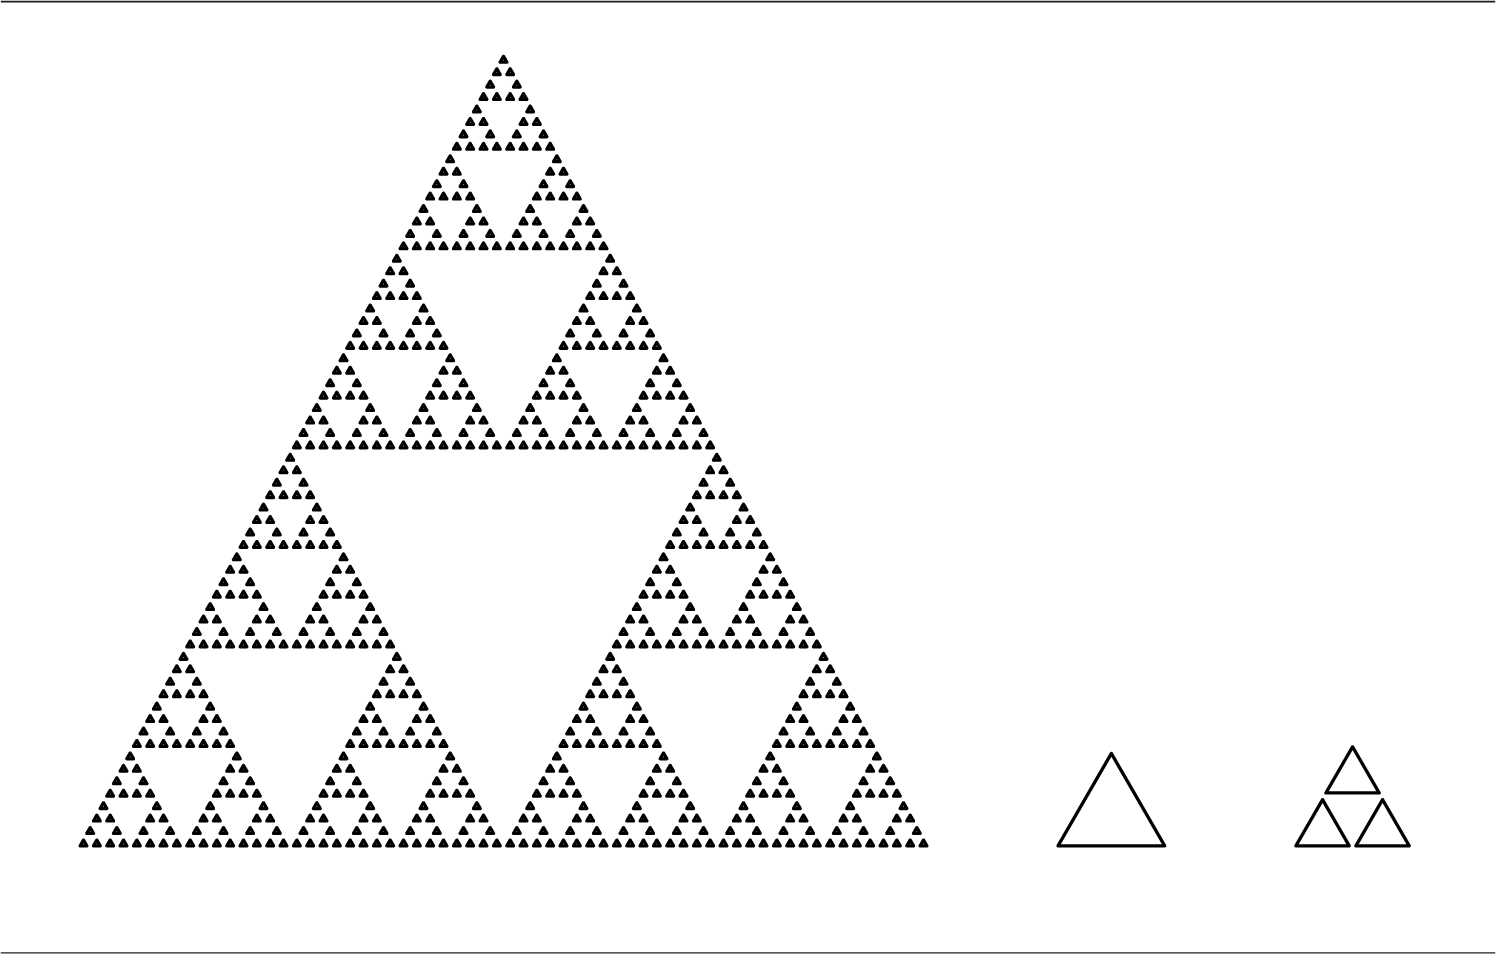
\includegraphics[width=0.8\textwidth]{images/00600.png}
  \caption{谢尔宾斯基三角形及其构造过程}
  \label{fig:sierpinski-triangle}
\end{figure}

图~\ref{fig:sierpinski-triangle} 最右侧的图像揭示了其生成步骤：给定一个大正三角形，找到各边的中点并将它们相互连结。这一步将大三角形划分为四个较小的全等三角形；只要小三角形的大小尚未达到视力或像素极限，就对除中心之外的三个外侧小三角形递归重复该过程。

另一种极为契合 \code{2htdp/image} 图像库组合函数的思路，基于从中间单三角形到右侧组合结构的过渡：将两个半尺寸的三角形水平并排（\code{beside}），然后在其上方居中放置一个相同的三角形（\code{above}），就能组合出大一号的双倍尺寸三角形：

\begin{lstlisting}[language=BSL]
(above half-sized
       (beside half-sized half-sized))
\end{lstlisting}

本节采用后一种自底向上的生成视角来设计谢尔宾斯基算法；第 34.3 节将使用前一种视角。由于目标是生成一个正三角形图像，我们用正数（三角形的边长 \code{side}）来表示该问题。这一决定给出了签名、目的说明与函数头：

\begin{lstlisting}[language=BSL]
; Number -> Image
; 生成边长为 side 的谢尔宾斯基三角形
(define (sierpinski side)
  (triangle side 'outline 'red))
\end{lstlisting}

现在我们来回答生成型递归的四个核心问题：
\begin{enumerate}
  \item \textbf{何为平凡问题？} 当给定的边长非常微小，以至于在其内部绘制更小的三角形已毫无意义时（例如小于阈值 \code{SMALL}），问题是平凡的。
  \item \textbf{平凡问题如何求解？} 此时只需直接画一个边长为 \code{side} 的基本正三角形即可。
  \item \textbf{如何生成新子问题？} 算法生成一个边长为 \code{side / 2} 的谢尔宾斯基三角形，因为三个这样的半尺寸三角形恰好能拼装出一个边长为 \code{side} 的新三角形。
  \item \textbf{如何合并子问题的解？} 若 \code{half-sized} 是边长为 \code{side / 2} 的谢尔宾斯基三角形图像，则表达式：
\begin{lstlisting}[language=BSL]
(above half-sized
       (beside half-sized half-sized))
\end{lstlisting}
  即为边长为 \code{side} 的谢尔宾斯基三角形。
\end{enumerate}

有了这些明确答案，定义函数便水到渠成。图~\ref{fig:sierpinski-code} 给出了完整实现。代码将平凡条件表达为 \code{(<= side SMALL)}，其中 \code{SMALL} 是一个预先定义的常数。在递归分支中，\code{local} 表达式引入局部变量 \code{half-sized} 保存递归调用生成的一半尺寸的谢尔宾斯基三角形，随后通过 \code{above} 和 \code{beside} 完成图元拼装。

\begin{figure}[htbp]
  \centering
\begin{lstlisting}[language=BSL]
(define SMALL 4) ; 像素级的微小尺寸阈值

(define small-triangle (triangle SMALL 'outline 'red))

; Number -> Image
; 生成型递归：生成边长为 side 的谢尔宾斯基三角形
; 方式：递归生成边长为 (/ side 2) 的半尺寸三角形，并将一个副本置于两个副本之上
(check-expect (sierpinski SMALL) small-triangle)
(check-expect (sierpinski (* 2 SMALL))
              (above small-triangle
                     (beside small-triangle small-triangle)))

(define (sierpinski side)
  (cond
    [(<= side SMALL) (triangle side 'outline 'red)]
    [else
     (local ((define half-sized (sierpinski (/ side 2))))
       (above half-sized
              (beside half-sized half-sized)))]))
\end{lstlisting}
  \caption{谢尔宾斯基三角形生成算法}
  \label{fig:sierpinski-code}
\end{figure}

最后进行终止性论证：\code{sierpinski} 的输入是一个正数 \code{side}。若该数值不大于正阈值 \code{SMALL}，算法直接终止；否则，递归调用接收的参数严格为当前边长的一半。只要初始边长与 \code{SMALL} 均为正数，连续除以 2 必然在有限步后进入小于等于 \code{SMALL} 的区间。因此该算法对于所有正数输入必然停机。

谢尔宾斯基算法的核心机制是：\textbf{不断将问题规模折半，直至可以直接求解}。稍加联想，你就会发现这种“区间折半”的过程可以用来极为高效地搜索满足特定性质的数值。下一节将深入剖析这一思想。

\section{二分搜索}
\label{sec:27_2}

应用数学家经常使用非线性方程对现实世界建模，并致力于求解这些方程。具体而言，他们将实际问题转化为从实数到实数的数学函数 $f$，并寻找某个实数 $r$ 满足：
\[ f(r) = 0 \]
这个数值 $r$ 被称为函数 $f$ 的\term{零点（root，或根）}。

\begin{notebox}[物理样例问题]
一枚火箭以 $v$ 英里/小时的恒定速度沿着直线向 $d_0$ 英里外的目标飞行。随后它以 $a$ 英里/小时$^2$ 的加速度加速飞行 $t$ 小时。火箭何时击中目标？
\end{notebox}

经典物理学告诉我们，火箭飞行的距离是时间的函数：
\[ d(t) = v \cdot t + \frac{1}{2} a \cdot t^2 \]
火箭击中目标的时刻就是剩余距离为 0 的时刻，即求解满足下式的 $t_0$：
\[ d_0 - \left(v \cdot t_0 + \frac{1}{2} a \cdot t_0^2\right) = 0 \]
初等代数告诉我们这是一个一元二次方程，在满足判别式条件时可用求根公式精确求解。

然而在工程实际中，问题往往远比二次方程复杂，很多方程根本不存在解析解。为此，数学家发展了多种针对不同连续函数的数值求根算法。本节探讨基于微积分早期核心定理——\term{介值定理（Intermediate Value Theorem, IVT，又称中间值定理）}的数值解法。这一算法是源自数学定理的生成型递归的典范。计算机科学家进一步将其推广为通用的\term{二分搜索（binary search）}算法。

\begin{notebox}[介值定理 (IVT)]
若实数函数 $f$ 在闭区间 $[a, b]$ 上是连续的，且 $f(a)$ 与 $f(b)$ 位于 $x$ 轴两侧（即一正一负，符号相异），则在区间 $[a, b]$ 内至少存在一点 $r$ 使得 $f(r) = 0$。
\end{notebox}

这里的“连续”直观上意味着函数图像是一条没有间断、跳跃和断裂的平滑曲线。图~\ref{fig:ivt-plot} 展现了介值定理的直观几何意义：函数 $f$ 在 $a$ 处位于 $x$ 轴下方，在 $b$ 处位于 $x$ 轴上方，因此其曲线必然在 $[a, b]$ 区间（图中标注为“range 1”）内横截穿过 $x$ 轴。

\begin{figure}[htbp]
  \centering
  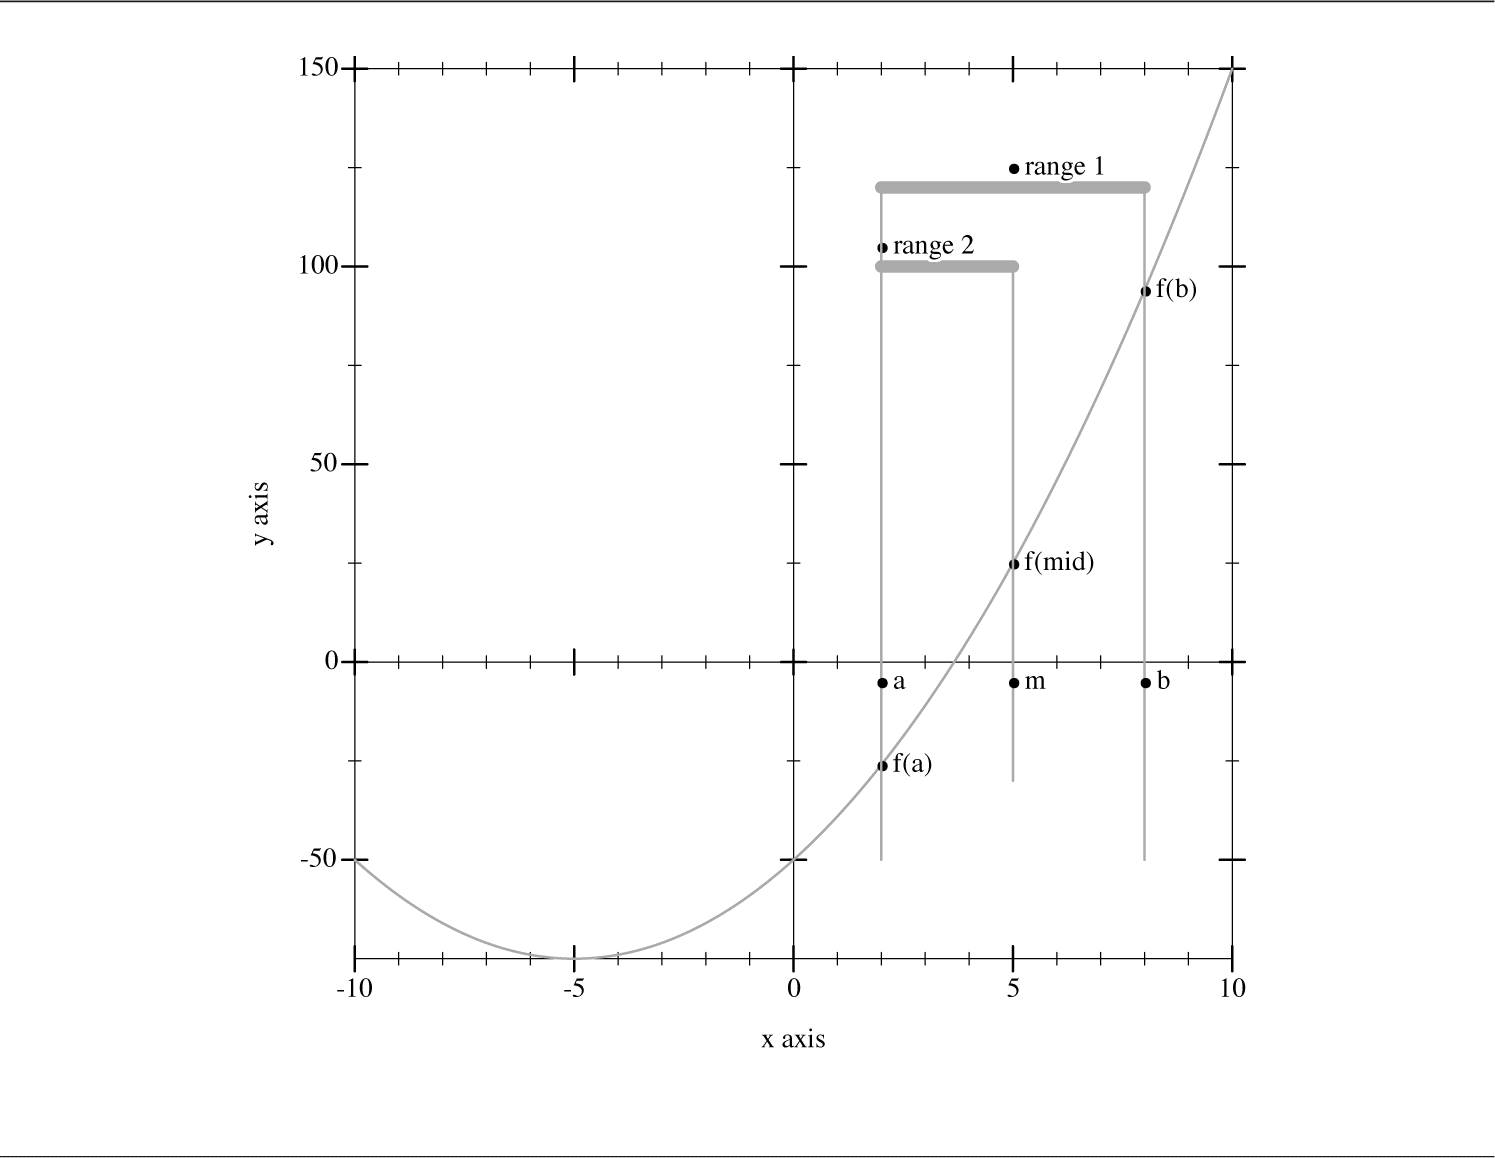
\includegraphics[width=0.8\textwidth]{images/00607.png}
  \caption{连续函数 $f$ 在区间 $[a, b]$ 内存在零点}
  \label{fig:ivt-plot}
\end{figure}

现在考察区间 $[a, b]$ 的中点（midpoint）：
\[ m = \frac{a + b}{2} \]
中点 $m$ 将大区间划分为两个长度减半的子区间：$[a, m]$ 与 $[m, b]$。计算中点处的函数值 $f(m)$：
\begin{itemize}
  \item 若 $f(m)$ 与 $f(a)$ 异号（即介值定理条件在左侧成立），则零点必定位于左半区间 $[a, m]$ 内（如图~\ref{fig:ivt-plot} 中的“range 2”所示）；
  \item 若 $f(m)$ 与 $f(b)$ 异号，则零点必定位于右半区间 $[m, b]$ 内。
\end{itemize}

我们现在有了求根核心步骤的清晰构想。接下来将其设计为 ISL+ 算法。算法接收一个数学函数以及预期包含零点的区间两端端点：

\begin{lstlisting}[language=BSL]
; [Number -> Number] Number Number -> Number
; 寻找 R 使得 f 在区间 [R, (+ R ε)] 内存在零点
; 前置假设 1：f 是连续函数
; 前置假设 2：(or (<= (f left) 0 (f right)) (<= (f right) 0 (f left)))
; 生成型递归：将区间折半，零点必在其中一半，依据假设 2 选择包含零点的那一半递归
(define (find-root f left right)
  0)
\end{lstlisting}

这里的 $\varepsilon$（可写为 \code{EPSILON}）是允许的误差阈值。随着搜索将区间不断折半，当区间跨度 \code{(- right left)} 缩小至不超过 $\varepsilon$ 时，搜索即告完成，此时返回区间的左端点 \code{left} 作为根的近似值。

\begin{exercise}{手算验证 poly 二项式求根}{445}\label{ex:445}
考虑多项式函数定义：
\begin{lstlisting}[language=BSL]
; Number -> Number
(define (poly x)
  (* (- x 2) (- x 4)))
\end{lstlisting}
这是一个二次函数，其解析根显然为 2 与 4。
\begin{enumerate}
  \item 利用 \code{poly} 为 \code{find-root} 设计一个基于 \code{check-satisfied} 的自动化测试。
  \item 以初始区间 $[3, 6]$ 和误差 $\varepsilon = 0$ 为例，按表格逐步记录二分求根的推演过程：列出每次迭代的 \code{left}、\code{right}、\code{mid}、$f(mid)$ 以及下一步选取的区间。
\end{enumerate}
\end{exercise}

针对算法设计的四个核心问题：
\begin{enumerate}
  \item \textbf{平凡情形判断}：当 \code{(<= (- right left) ε)} 时，区间跨度已在容差范围内，问题平凡解决。
  \item \textbf{平凡解}：直接返回当前的 \code{left} 端点。
  \item \textbf{生成子问题}：计算中点 \code{mid = (/ (+ left right) 2)} 及其函数值 \code{f@m = (f mid)}。若 \code{f(left)} 与 \code{f@m} 异号，生成左半区间 \code{[left, mid]}；否则生成右半区间 \code{[mid, right]}。
  \item \textbf{合并子问题的解}：子问题找到的根直接就是原问题的根，无需后处理合并。
\end{enumerate}

图~\ref{fig:find-root-code} 给出了 \code{find-root} 的完整实现。

\begin{figure}[htbp]
  \centering
\begin{lstlisting}[language=BSL]
(define ε 0.001)

; [Number -> Number] Number Number -> Number
; 确定 R 使得 f 在 [R, (+ R ε)] 内有根
; 假设 f 连续，且 f(left) 与 f(right) 在 x 轴两侧
(define (find-root f left right)
  (cond
    [(<= (- right left) ε) left]
    [else
     (local ((define mid (/ (+ left right) 2))
             (define f@mid (f mid)))
       (cond
         [(or (<= (f left) 0 f@mid) (<= f@mid 0 (f left)))
          (find-root f left mid)]
         [else
          (find-root f mid right)]))]))
\end{lstlisting}
  \caption{二分法求根算法}
  \label{fig:find-root-code}
\end{figure}

\begin{exercise}{验证 find-root 并在不同容差下实验}{446}\label{ex:446}
将练习~\ref{ex:445} 中的测试用例加入到图~\ref{fig:find-root-code} 的程序中。尝试不同的 $\varepsilon$ 取值（如 0.1, 0.001, 0.00001），观察近似结果精度的变化。
\end{exercise}

\begin{exercise}{包含两个零点的区间}{447}\label{ex:447}
多项式 \code{poly} 拥有两个零点（2 和 4）。如果在调用 \code{find-root} 时传入同时包含这两个零点的区间（例如 $[1, 5]$），函数会返回哪一个零点？为什么？
\end{exercise}

\begin{exercise}{find-root 的终止性论证与收敛速度}{448}\label{ex:448}
论证 \code{find-root} 对于所有满足前置假设的连续函数与初值必能停机。假设初始区间跨度为 $S$。第 $k$ 次递归调用时的区间跨度是多少？经过多少次递归调用后必有 $(- \text{right}\ \text{left}) \le \varepsilon$？
\end{exercise}

\begin{exercise}{消除函数值的重复计算与累加器雏形}{449}\label{ex:449}
仔细观察图~\ref{fig:find-root-code}：\code{find-root} 在每个阶段都对端点重复计算 $f$ 的值。例如在跨越递归调用时，若选择了 $[left, mid]$，下一次调用又会重新计算 $(f\ left)$。
\begin{enumerate}
  \item 先利用 \code{local} 消除同一次调用内部重复求值的问题。
  \item 进一步设计一个辅助函数：它不仅接收 \code{left} 和 \code{right}，还接收前一次计算好的 $(f\ left)$ 与 $(f\ right)$ 作为参数传递给下一步。
\end{enumerate}
这种随数值递归同步传递已计算结果的技术，就是第 VI 部分的主题——\term{累加器（accumulators）}。
\end{exercise}

\begin{exercise}{单调函数的二分求根简化}{450}\label{ex:450}
如果函数 $f$ 是单调递增的（即当 $a < b$ 时恒有 $f(a) \le f(b)$），请简化 \code{find-root} 中的符号判断逻辑。
\end{exercise}

\begin{exercise}{表结构的线性搜索与二分搜索对比}{451}\label{ex:451}
定义结构体 \code{table} 包含两个字段：长度 \code{length} 与函数 \code{array}。该函数接收自然数索引并返回对应数值：
\begin{lstlisting}[language=BSL]
(define-struct table [length array])
; Table 是结构体：(make-table N [N -> Number])
\end{lstlisting}
表检索辅助函数定义为：
\begin{lstlisting}[language=BSL]
; Table N -> Number
; 查询表 t 中索引为 i 的数值
(define (table-ref t i)
  ((table-array t) i))
\end{lstlisting}
表的零点索引是指满足 \code{(table-ref t i)} 最接近 0 的自然数 $i$。
\begin{enumerate}
  \item 设计 \code{find-linear}：对单调递增的表，使用从 0 递增到 \code{length} 的结构型递归进行\term{线性搜索}。
  \item 设计 \code{find-binary}：使用基于二分搜索的生成型递归快速定位零点索引，并为其撰写终止性论证。
  \item 设表长度为 1024，零点在 1023 处。分别计算 \code{find-linear} 与 \code{find-binary} 所需的查询次数。
\end{enumerate}
\end{exercise}

\section{解析初窥}
\label{sec:27_3}

计算机系统通过文件提供持久化存储。在我们的计算模型中，文件本质上就是一个包含单字符字符串（\code{1String}）的列表，其中夹杂着特殊的换行符：

\begin{lstlisting}[language=BSL]
; File 是以下之一：
; -- '()
; -- (cons "\n" File)
; -- (cons 1String File)
; 解释：表示文本文件的内容，"\n" 代表换行字符

; Line 是 [List-of 1String]
\end{lstlisting}

许多程序需要将文件按行处理。例如 \code{2htdp/batch-io} 库中的 \code{read-lines} 函数，其任务就是将如下格式的文件列表：
\begin{lstlisting}[language=BSL]
(list "h" "o" "w" " " "a" "r" "e" " " "y" "o" "u" "\n"
      "d" "o" "i" "n" "g" "?" "\n"
      "a" "n" "y" " " "p" "r" "o" "g" "r" "e" "s" "s" "?")
\end{lstlisting}
转换为由三行构成的列表：
\begin{lstlisting}[language=BSL]
(list (list "h" "o" "w" " " "a" "r" "e" " " "y" "o" "u")
      (list "d" "o" "i" "n" "g" "?")
      (list "a" "n" "y" " " "p" "r" "o" "g" "r" "e" "s" "s" "?"))
\end{lstlisting}

将离散的符号序列转换为结构化分层数据的过程称为\term{解析（parsing）}。实际应用中需要解析单词、数字以及语法树（词法分析与语法分析）。

对于将 \code{File} 转换为 \code{[List-of Line]} 的函数 \code{file->list-of-lines}，运用生成型递归的四个问题分析如下：
\begin{enumerate}
  \item 当文件为空列表 \code{'()} 时，问题平凡，返回 \code{'()}；
  \item 否则，文件包含至少一个字符或换行符。算法必须提取出首个换行符之前的所有字符作为“第一行”（\code{Line}）；
  \item 剥离掉首行及换行符之后剩余的部分构成同类的新子问题，递归调用 \code{file->list-of-lines} 予以解决；
  \item 最后，使用 \code{cons} 将第一行与剩余行列表组合起来。
\end{enumerate}

这一思路清晰表明我们需要两个结构型递归辅助函数：
\begin{itemize}
  \item \code{first-line}：收集遇到的第一个 \code{"\textbackslash n"} 之前的所有字符；
  \item \code{remove-first-line}：丢弃第一个 \code{"\textbackslash n"} 及其之前的所有字符，返回剩余文件内容。
\end{itemize}

图~\ref{fig:file-lines-code} 展示了完整代码。

\begin{figure}[htbp]
  \centering
\begin{lstlisting}[language=BSL]
; File -> [List-of Line]
; 将一个文本文件内容转化为行列表
(define (file->list-of-lines afile)
  (cond
    [(empty? afile) '()]
    [else
     (cons (first-line afile)
           (file->list-of-lines (remove-first-line afile)))]))

; File -> Line
; 提取文件首个换行符之前的所有字符
(define (first-line afile)
  (cond
    [(empty? afile) '()]
    [(string=? (first afile) "\n") '()]
    [else (cons (first afile) (first-line (rest afile)))]))

; File -> File
; 剔除文件第一行（包括换行符）并返回剩余文件
(define (remove-first-line afile)
  (cond
    [(empty? afile) '()]
    [(string=? (first afile) "\n") (rest afile)]
    [else (remove-first-line (rest afile))]))
\end{lstlisting}
  \caption{将文本文件转换为行列表的解析算法}
  \label{fig:file-lines-code}
\end{figure}

注意在 \code{file->list-of-lines} 中，传给递归调用的实参是 \code{(remove-first-line afile)}，绝非简单的 \code{(rest afile)}。由于每次至少移除了一个字符（或一行），子问题的文件长度严格缩短，因此算法必定停机。

\begin{exercise}{完善辅助函数的目的说明}{452}\label{ex:452}
为图~\ref{fig:file-lines-code} 中的 \code{first-line} 和 \code{remove-first-line} 编写规范、精准的目的说明与单元测试。
\end{exercise}

\begin{exercise}{分词器 tokenize 的设计}{453}\label{ex:453}
设计函数 \code{tokenize}，将一行字符（\code{Line}）拆分为记号（token）列表。在这里，记号要么是标点等单字符，要么是由连续小写英文字母组成的单词（\code{String}）。所有空白字符均被剔除。提示：参考 \code{string-whitespace?} 函数。
\end{exercise}

\begin{exercise}{矩阵构造函数 create-matrix}{454}\label{ex:454}
设计函数 \code{create-matrix}。它接收数字 $n$ 以及包含 $n^2$ 个数值的列表，生成一个 $n \times n$ 的嵌套列表矩阵。例如：
\begin{lstlisting}[language=BSL]
(check-expect
  (create-matrix 2 '(1 2 3 4))
  (list (list 1 2)
        (list 3 4)))
\end{lstlisting}
再编写至少两个测试用例，并运用生成型递归实现该函数。
\end{exercise}

% ==============================================================================
% 第 28 章：数学实例 (Chapter 28: Mathematical Examples)
% ==============================================================================

\chapter{数学实例}
\label{sec:ch28_math}

许多数学问题的计算机求解都深刻依赖于生成型递归。未来的软件工程师必须熟练掌握这些经典解法，其原因有二：一方面，相当一部分实际编程任务本质上就是将这类数学思想转化为高效程序；另一方面，在数学问题上的思维训练往往能为算法设计提供极具启发性的灵感源泉。本章将深入研讨三个此类核心经典问题：牛顿求根法、数值积分以及高斯消元法。

\section{牛顿法}
\label{sec:28_1}

第 27.2 节介绍了寻找数学函数零点的一种方法（二分法）。在纯粹的数学与科学计算领域，程序员更倾向于采用源自微积分分析的高效方法，其中最著名的当属\term{牛顿法（Newton's method）}。与二分法类似，牛顿法通过反复迭代来逐步改进对零点的近似值，直至足够逼近目标。

从一个初始猜测值 $r_1$ 出发，牛顿法的核心计算过程在于：\textbf{构造函数 $f$ 在点 $r_1$ 处的切线（tangent），并求解该切线的零点}。由于切线在局部线性逼近了原函数，而求解一条直线的零点极为简便，通过充分多次重复该迭代过程，算法通常能够迅速收敛到一个使得 $f(r)$ 极其接近 0 的精确数值 $r$。

显然，这一过程依赖于有关切线的两项数学领域知识：其斜率与零点。直观上，函数 $f$ 在点 $r_1$ 处的切线是穿过点 $(r_1, f(r_1))$ 且与曲线 $f$ 具有相同斜率的直线。在数值计算中，获取切线斜率的一种标准方式是在 $x$ 轴上选取关于 $r_1$ 对称的两个微小间距点：$r_1 - \varepsilon$ 与 $r_1 + \varepsilon$（其中 $\varepsilon$ 是一个充分小的正常数）。由两点 $(r_1 - \varepsilon, f(r_1 - \varepsilon))$ 和 $(r_1 + \varepsilon, f(r_1 + \varepsilon))$ 确定的割线斜率即可作为切线斜率的高精度近似：
\[ \text{slope} = \frac{f(r_1 + \varepsilon) - f(r_1 - \varepsilon)}{2\varepsilon} \]

\begin{exercise}{数值导数与斜率函数 slope}{455}\label{ex:455}
将上述数学公式翻译为 ISL+ 函数 \code{slope}。它接收函数 $f$ 与数值 $r_1$，输出 $f$ 在 $r_1$ 处的数值斜率。假设 $\varepsilon$ 为全局常量。编写测试用例验证水平线、线性函数以及简单多项式的斜率计算。
\end{exercise}

第二项领域知识是切线的零点。切线本身是一条直线（线性函数），它经过点 $(r_1, f(r_1))$ 且具有斜率 $m = \text{slope}$。在数学上，其方程可表示为：
\[ \text{tangent}(x) = f(r_1) + m \cdot (x - r_1) \]
寻找切线的零点即求解方程 $\text{tangent}(\text{root-of-tangent}) = 0$：
\[ f(r_1) + m \cdot (\text{root-of-tangent} - r_1) = 0 \]
直接求解该一元一次方程可得：
\[ \text{root-of-tangent} = r_1 - \frac{f(r_1)}{m} \]

\begin{exercise}{切线零点函数 root-of-tangent}{456}\label{ex:456}
设计函数 \code{root-of-tangent}，它接收函数 $f$ 与数值 $r_1$，计算通过点 $(r_1, f(r_1))$ 的切线的零点。
\end{exercise}

现在依照生成型递归的设计配方来实现牛顿法。函数 \code{newton} 接收待求根函数 $f$ 与初始猜测 $r_1$：

\begin{lstlisting}[language=BSL]
; [Number -> Number] Number -> Number
; 寻找数值 r 使得 (f r) 接近 0
; 生成型递归：反复生成改进后的猜测值
(define (newton f r1) 1.0)
\end{lstlisting}

回答四个核心设计问题：
\begin{enumerate}
  \item \textbf{平凡情形判断}：当 $|f(r_1)| \le \varepsilon$ 时，当前猜测已足够精确，问题已解。
  \item \textbf{平凡解}：直接返回 $r_1$。
  \item \textbf{生成子问题}：计算 $f$ 在 $r_1$ 处切线的零点作为下一次更优的猜测值，即 \code{(root-of-tangent f r1)}，并以该新值递归调用 \code{newton}。
  \item \textbf{合并解}：递归子问题的解直接就是原问题的解。
\end{enumerate}

图~\ref{fig:newton-code} 展示了 \code{newton} 的完整实现。

\begin{figure}[htbp]
  \centering
\begin{lstlisting}[language=BSL]
; [Number -> Number] Number -> Number
; 寻找数值 r 使得 (<= (abs (f r)) ε)
(check-within (newton poly 1) 2 ε)
(check-within (newton poly 3.5) 4 ε)

(define (newton f r1)
  (cond
    [(<= (abs (f r1)) ε) r1]
    [else (newton f (root-of-tangent f r1))]))
\end{lstlisting}
  \caption{牛顿法求根程序}
  \label{fig:newton-code}
\end{figure}

此时设计并未结束。配方的第七步要求深入剖析牛顿法的停机性。对于如下二次多项式：
\begin{lstlisting}[language=BSL]
; Number -> Number
(define (poly x) (* (- x 2) (- x 4)))
\end{lstlisting}
其真根为 2 和 4。图~\ref{fig:poly-graph} 展示了 \code{poly} 的曲线：它在对称轴 $x = 3$ 处达到极小值，切线完全水平（斜率为 0）。

\begin{figure}[htbp]
  \centering
  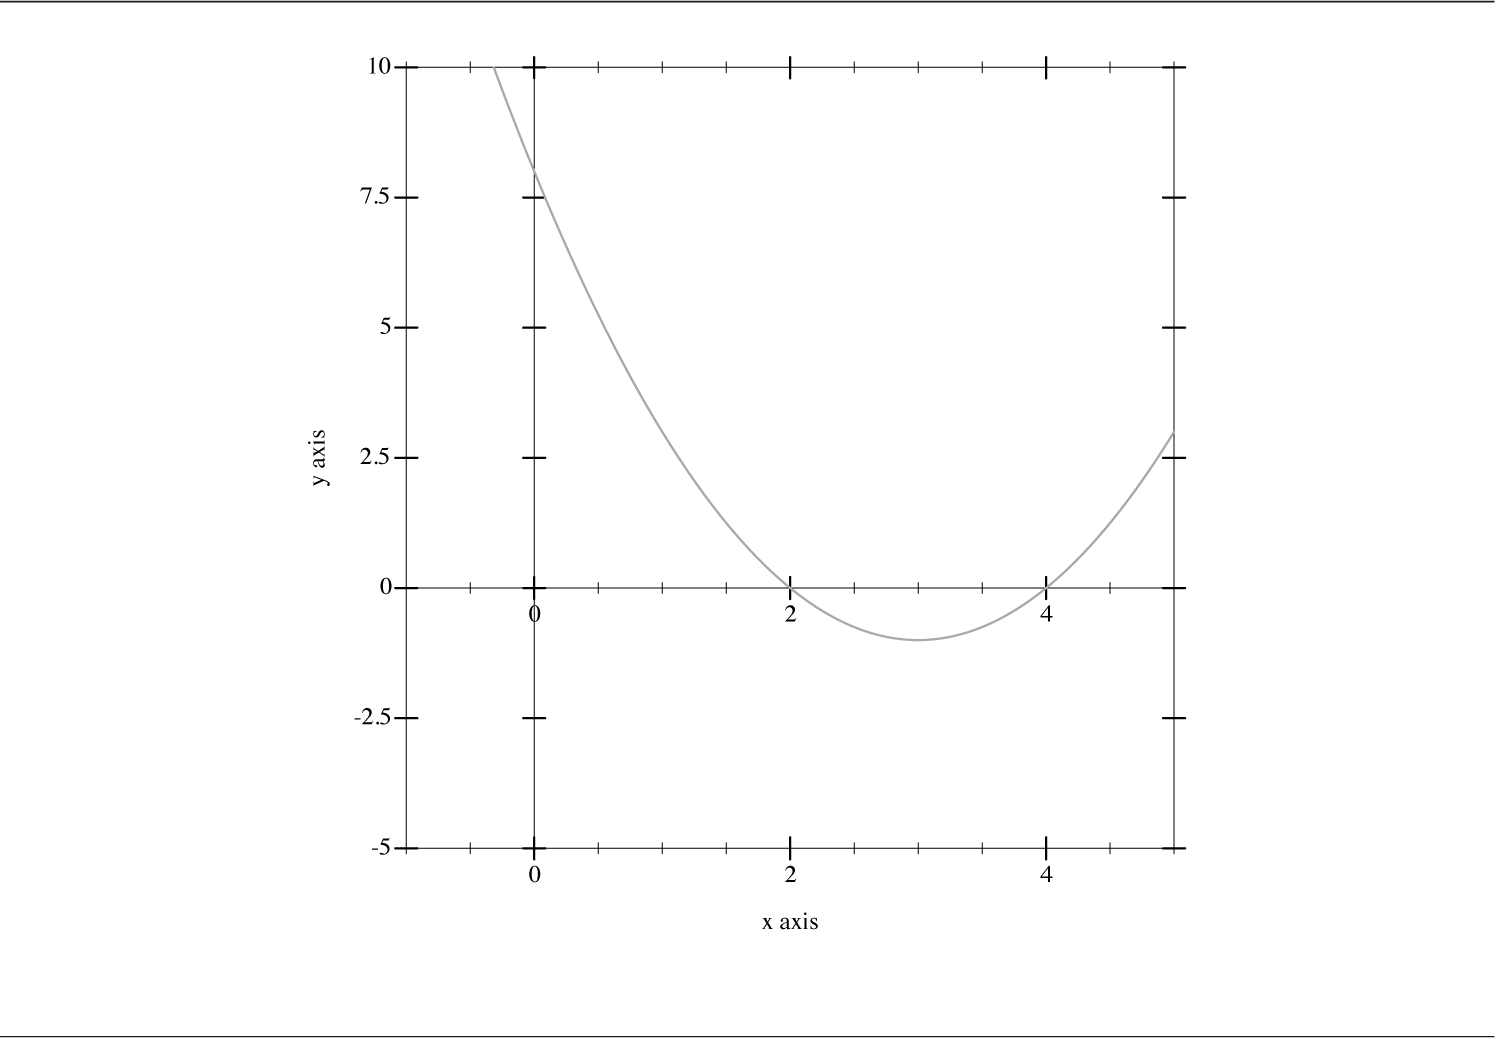
\includegraphics[width=0.75\textwidth]{images/00623.png}
  \caption{\code{poly} 在区间 $[-1, 5]$ 上的图像}
  \label{fig:poly-graph}
\end{figure}

如果以 3 作为初始猜测调用 \code{newton}，计算将会崩溃：
\begin{lstlisting}[language=BSL]
> (poly 3)
-1
> (newton poly 3)
/: division by zero
\end{lstlisting}
原因在于此时切线斜率为 0，除以斜率引发了除零异常。

除了除零错误之外，牛顿法还暴露了与数值精度相关的另外两个严峻停机性问题：
\begin{itemize}
  \item \textbf{精确有理数运算导致的假性“挂起”}：如果在 DrRacket 中传入精确浮点数 \code{2.9999}，ISL+ 会将其作为精确有理分数（如 $29999/10000$）进行无损分数算术。随着连续求导与分式计算，分母与分子的位宽会以指数级爆炸膨胀，导致运算速度急剧下降，耗费数分钟甚至让人误以为程序已经陷入死循环。
  \item \textbf{不精确浮点数导致的发散死循环}：若传入不精确数 \code{\#i3.0}，由于浮点除零会产生 \code{\#i+inf.0}（无穷大），进而参与后续运算产生 \code{\#i+nan.0}（非数），程序将彻底跌入无限递归死循环。
\end{itemize}

因此，编写科学计算函数时，必须在文档和函数头中极为审慎地注明这些收敛陷阱与停机前置条件。

\begin{exercise}{72 法则与资金翻倍计算}{457}\label{ex:457}
设计函数 \code{double-amount}，计算当储蓄账户按月以固定月利率计息时，一笔本金翻倍所需经历的月数。通过代数化简证明本金具体数额无关紧要，仅利率起决定性作用；并验证金融学中著名的“72 法则”（即翻倍月数约为 $72/r$）。
\end{exercise}

\section{数值积分}
\label{sec:28_2}

诸多物理学与工程问题的本质都可归结为计算曲线下方的面积：
\begin{notebox}[物理样例问题]
一辆汽车以恒定速度 $v$ 米/秒行驶，在 5 秒、10 秒、15 秒后行驶的位移是多少？一架火箭以恒定加速度 $a = 12\text{ m/s}^2$ 垂直发射升空，在 5 秒、10 秒、15 秒后达到的高度是多少？
\end{notebox}

物理学定律表明，匀速运动的位移等于矩形面积 $d_{\text{con}}(t) = v \cdot t$；而匀加速运动的位移则对应于三角形面积 $d_{\text{acc}}(t) = \frac{1}{2} a \cdot t^2$。在更广泛的物理世界中，物体在一段时间内运动的位移，严格对应于其速度函数曲线与时间轴之间所围成的曲边梯形面积，如图~\ref{fig:motion-integral} 所示。在给定区间内确定函数图像下方所围面积的计算过程被称为\term{数值积分（numeric integration）}。

\begin{figure}[htbp]
  \centering
  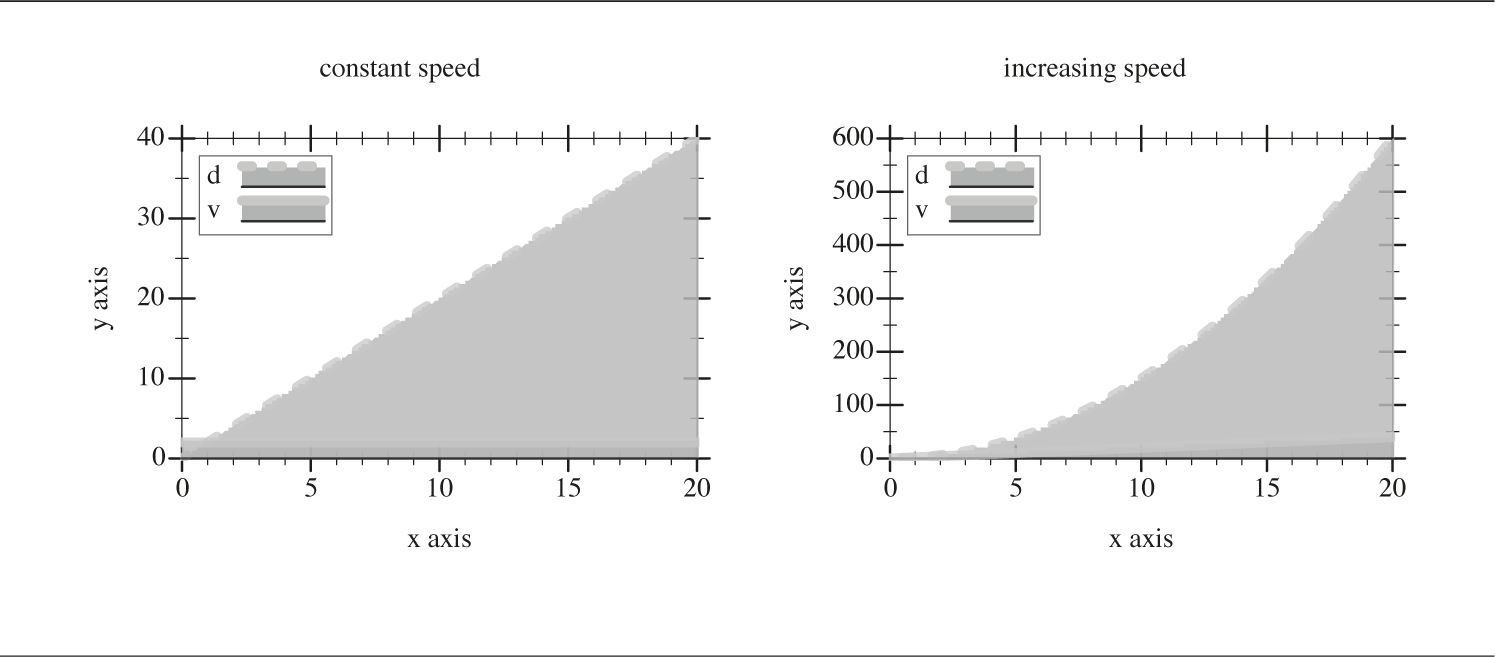
\includegraphics[width=0.85\textwidth]{images/00625.jpeg}
  \caption{匀速行驶与加速行驶中的位移与曲线下面积}
  \label{fig:motion-integral}
\end{figure}

对于任意复杂的曲线（如图~\ref{fig:integral-sketch} 所示），数学解析积分往往极难甚至不可行。计算机科学通过数值近似算法，将曲边图形切分为成千上万个微小的基础几何图形（如矩形、梯形）并对其求和，从而以极高精度逼近积分面积。

\begin{figure}[htbp]
  \centering
  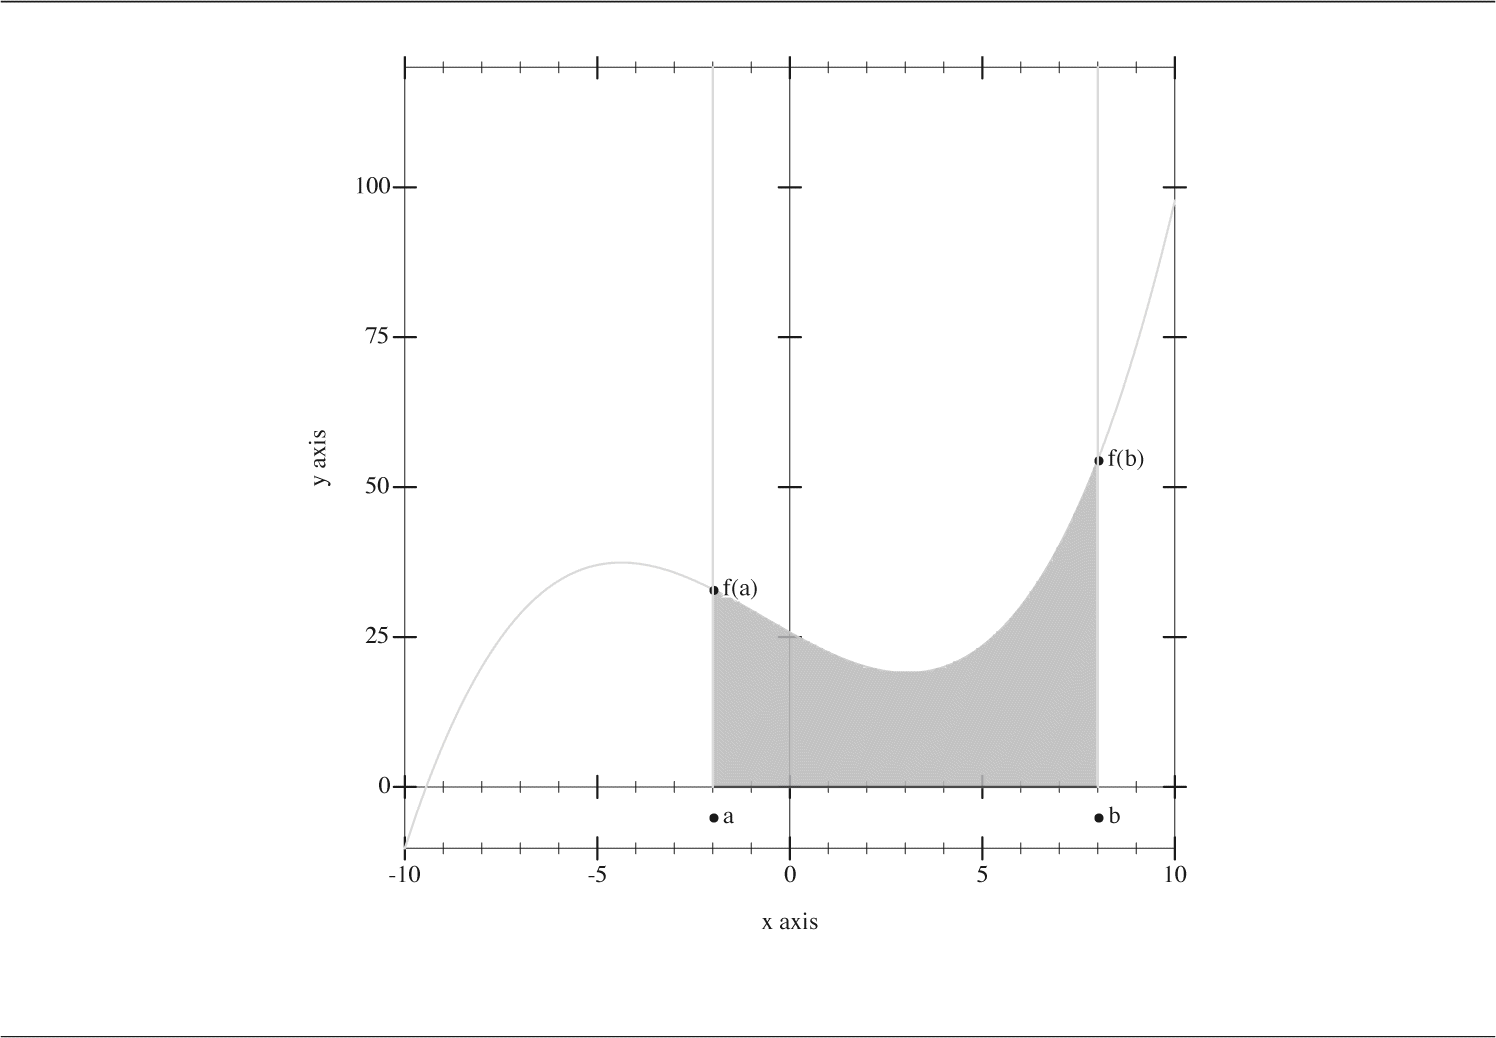
\includegraphics[width=0.75\textwidth]{images/00626.png}
  \caption{在区间 $[a, b]$ 上对函数 $f$ 进行数值积分}
  \label{fig:integral-sketch}
\end{figure}

数值积分函数接收被积函数 $f$ 以及积分区间的左右端点 $a$ 与 $b$：

\begin{lstlisting}[language=BSL]
; [Number -> Number] Number Number -> Number
\end{lstlisting}

图~\ref{fig:generic-integrate} 给出了前三个设计步骤的成果。考虑到浮点近似误差，测试用例统一使用 \code{check-within}，函数头返回 \code{\#i0.0} 显式标明其返回不精确数值。

\begin{figure}[htbp]
  \centering
\begin{lstlisting}[language=BSL]
(define ε 0.1)

; [Number -> Number] Number Number -> Number
; 计算函数 f 在区间 [a, b] 上与 x 轴所围成的面积
; 假设 (< a b) 成立

(check-within (integrate (lambda (x) 20) 12 22) 200 ε)
(check-within (integrate (lambda (x) (* 2 x)) 0 10) 100 ε)
(check-within (integrate (lambda (x) (* 3 (sqr x))) 0 10) 1000 ε)

(define (integrate f a b)
  #i0.0)
\end{lstlisting}
  \caption{通用数值积分函数签名与规范用例}
  \label{fig:generic-integrate}
\end{figure}

\begin{exercise}{开普勒梯形求积法}{458}\label{ex:458}
开普勒（Kepler）提出了一种简便的求积法则：将区间在 $\text{mid} = (a+b)/2$ 处一分为二，计算左侧和右侧两个梯形的面积并相加。梯形面积公式可统一表示为：
\[ \text{Area} = \frac{f(L) + f(R)}{2} \cdot (R - L) \]
设计函数 \code{integrate-kepler}，实现开普勒梯形法。在图~\ref{fig:generic-integrate} 的三个测试用例中，哪一个会出现显著误差？为什么？
\end{exercise}

\begin{exercise}{矩形中点法（黎曼和）}{459}\label{ex:459}
另一种经典数值积分法是将整个区间划分为 $R$ 个等宽的小矩形。每个矩形的宽度为 $W = (b-a)/R$，高度取矩形中点处的函数值 $f(a + (i + 0.5) \cdot W)$。所有矩形面积之和即为积分估计值。
设计函数 \code{integrate-rectangles}。将矩形数量 $R$ 设置为可调常量，观察当 $R$ 逐级提升（如 10, 100, 1000）时，近似精度是如何逼近真实值的。
\end{exercise}

\begin{exercise}{基于分治法的简单数值积分}{460}\label{ex:460}
结合二分折半策略开发函数 \code{integrate-dc}：递归将区间平分，分别计算左右两部分的积分值并相加。当区间跨度小于设定容差时，直接采用开普勒梯形公式。
\end{exercise}

简单的分治求积分（如练习~\ref{ex:460}）存在巨大的计算浪费：对于函数曲线平缓平坦的区域，盲目地深层细分区间不仅毫无必要，而且空耗算力；而对于曲线剧烈振荡震颤的区域（如图~\ref{fig:adaptive-sample} 所示），若不进行足够细致的切分，又会产生致命误差。

\begin{figure}[htbp]
  \centering
  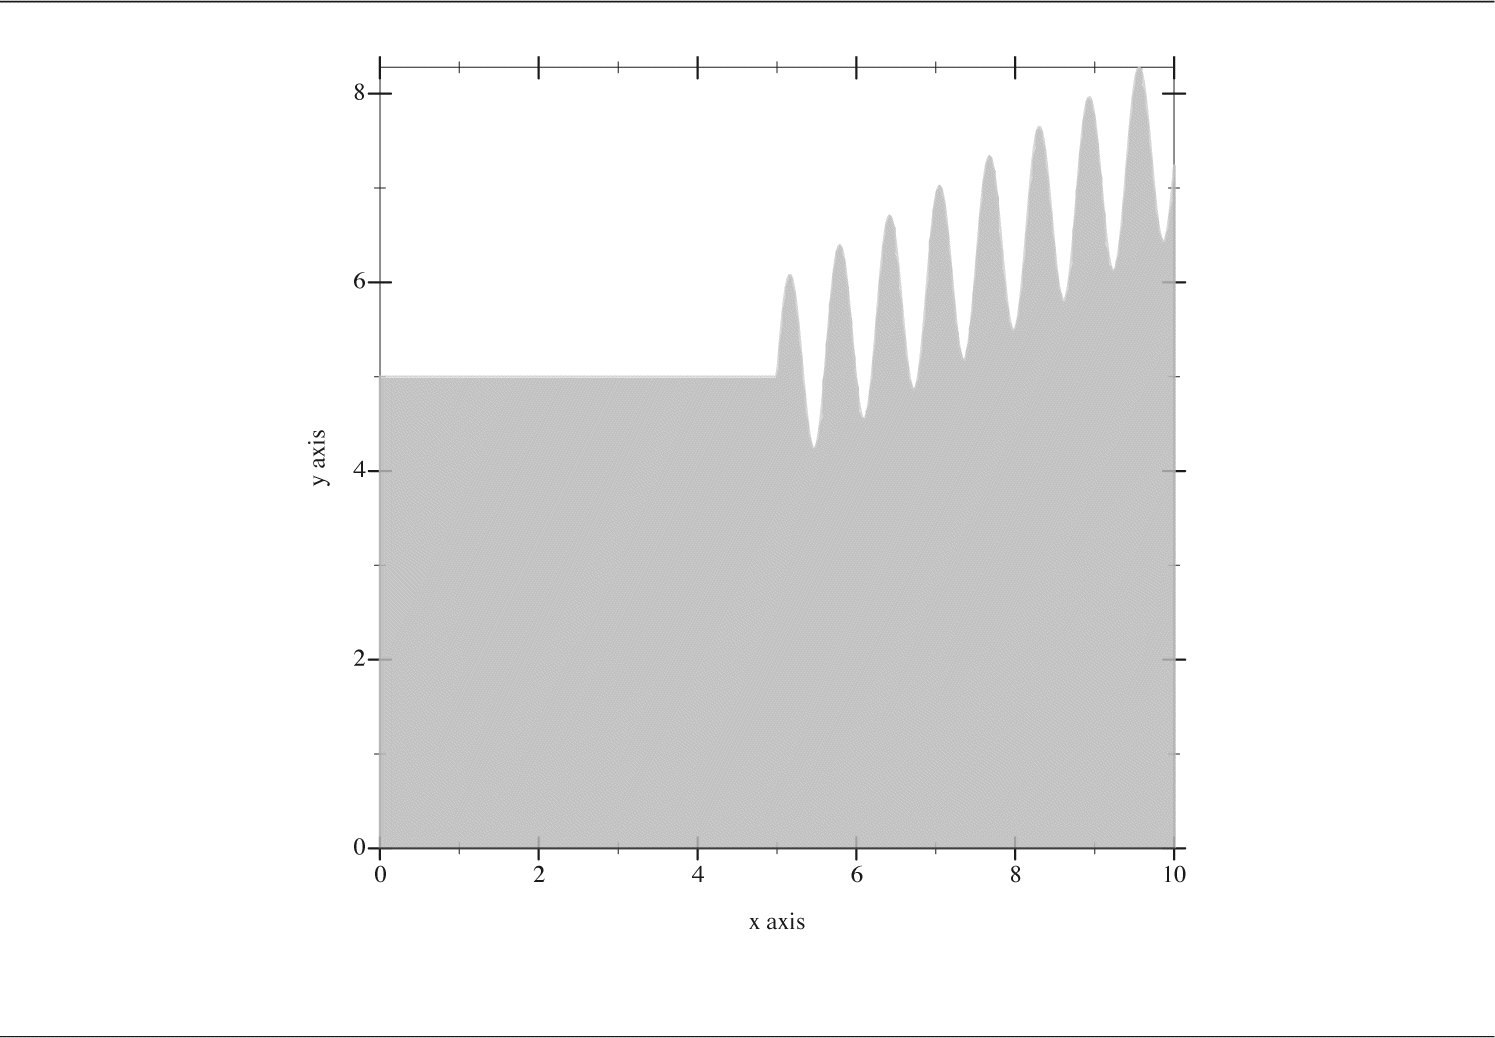
\includegraphics[width=0.75\textwidth]{images/00642.png}
  \caption{自适应积分候选函数：平缓区域与剧烈变动区域共存}
  \label{fig:adaptive-sample}
\end{figure}

为了智能探测函数在当前区域的平缓程度，算法可以计算三个梯形面积：大区间的梯形面积 $A_{\text{single}}$，以及左右两半区间的梯形面积之和 $A_{\text{split}} = A_{\text{left}} + A_{\text{right}}$。若两者的绝对偏差小于容许误差矩形 $\varepsilon \cdot (b - a)$：
\[ |A_{\text{single}} - A_{\text{split}}| \le \varepsilon \cdot (b - a) \]
则可断定当前区间的线性近似已足够优异，直接返回 $A_{\text{split}}$；否则，继续递归分治。这种能根据函数曲线形态\textbf{按需自动分配计算算力}的高级算法，被称为\term{自适应数值积分（adaptive numeric integration）}。

\begin{exercise}{自适应积分算法设计}{461}\label{ex:461}
设计函数 \code{integrate-adaptive}。在平缓区与剧烈变化区对比其实际递归深度与计算开销。为什么说自适应算法是现代计算软件中的必备利器？
\end{exercise}

\section{综合项目：高斯消元法}
\label{sec:28_3}

数学家不仅研究一元非线性方程，还广泛研究多元\term{线性方程组（system of linear equations, SOE）}：
\begin{notebox}[资源物物交换问题]
在物物交换经济中，煤炭（$x$）、石油（$y$）和天然气（$z$）的单位价值由如下三元一次方程组决定：
\begin{align*}
  2x + 2y + 3z &= 10 \\
  2x + 5y + 12z &= 31 \\
  4x + y - 4z &= -7
\end{align*}
\end{notebox}

方程组的解是一组数字 $(x=1, y=1, z=2)$，代入各个方程均能使得等式严格成立。

图~\ref{fig:soe-rep} 确立了该问题域的数据表示：我们用嵌套列表矩阵（\code{Matrix}）来表示方程组，其中每一行是一个方程（\code{Equation}），包含未知数的系数及等式右侧的常数项。

\begin{figure}[htbp]
  \centering
\begin{lstlisting}[language=BSL]
; SOE 是非空矩阵 [Matrix-of Number]
; 约束：对于 (list r1 ... rn)，每行长度 (length ri) 均为 (+ n 1)
; 解释：表示线性方程组

; Equation 是 [List-of Number]
; 约束：Equation 至少包含两个数字
; 解释：若 (list a1 ... an b) 是方程，则 a1 到 an 为系数，b 为等号右侧常数

; Solution 是 [List-of Number]

(define M
  (list (list 2 2  3 10)
        (list 2 5 12 31)
        (list 4 1 -4 -7)))

(define S '(1 1 2)) ; 解向量 (x=1, y=1, z=2)
\end{lstlisting}
  \caption{线性方程组的数据表示}
  \label{fig:soe-rep}
\end{figure}

提取方程左右两侧的工具函数定义如下：
\begin{lstlisting}[language=BSL]
; Equation -> [List-of Number]
(define (lhs e) (reverse (rest (reverse e))))

; Equation -> Number
(define (rhs e) (first (reverse e)))
\end{lstlisting}

\begin{exercise}{解的验证函数 check-solution}{462}\label{ex:462}
设计函数 \code{check-solution}，接收一个 \code{SOE} 和候选 \code{Solution}。当将解代入各方程后所有等式均成立时返回 \code{\#true}，否则返回 \code{\#false}。
\end{exercise}

\term{高斯消元法（Gaussian elimination）}由两阶段构成：第一阶段是\term{三角化（triangulation）}，通过行初等变换将矩形矩阵转化为同解的上三角矩阵；第二阶段是\term{回代求解（back-substitution）}，逐个回代未知数求出最终解。

三角化的生成式思想是：利用第一行方程作为基准（主元行），消去其余各行在第一列上的变量系数，使得除第一行外所有方程的首项系数均变为 0。在我们的样例中，第二行减去第一行得到：
\begin{lstlisting}[language=BSL]
'(0 3 9 21)
\end{lstlisting}
第三行减去第一行的 2 倍得到：
\begin{lstlisting}[language=BSL]
'(0 -3 -10 -27)
\end{lstlisting}
由于首列系数已经全为 0，按照消元惯例我们可以省略开头的 0，从而将剩余部分缩减为一个规模减小一维的子方程组：
\begin{lstlisting}[language=BSL]
'((3 9 21)
  (-3 -10 -27))
\end{lstlisting}
这是一个规模更小的同类子问题！再次执行生成型递归消元，即可获得最终优美的三角形方程组：
\begin{lstlisting}[language=BSL]
'((2 2 3 10)
  (3 9 21)
  (-1 -6))
\end{lstlisting}
此时 $z$ 的值由最后一行一目了然：$-z = -6 \implies z = 2$。

\begin{exercise}{行减法函数 subtract}{465}\label{ex:465}
设计函数 \code{subtract}。它接收两个等长的 \code{Equation}，从第一个方程中减去第二个方程的适当时倍数，使得结果方程首项系数恰为 0，并返回剔除首个 0 之后的剩余列表。
\end{exercise}

\begin{exercise}{初步三角化算法 triangulate}{466}\label{ex:466}
利用 \code{subtract} 设计生成型递归算法 \code{triangulate}，将合法系数的 \code{SOE} 转换为严格上三角矩阵 \code{TM}。
\end{exercise}

在消元过程中，有时会遭遇主元首项系数为 0 的异常情形。数学定理保证：交换方程组中两行的次序不改变其解集。因此，当首项系数为 0 时，可以通过\term{选主元（pivoting，或主元换行）}来寻找合适的主元行。

\begin{exercise}{带主元轮换的稳健三角化}{467}\label{ex:467}
完善 \code{triangulate}：在执行消元前先检查首项系数，若为 0 则通过轮转行列表找到首系数非零的方程置于首位。
\end{exercise}

\begin{exercise}{奇异与无解方程组的错误检测}{468}\label{ex:468}
某些方程组存在多重共线或相互矛盾，导致消元过程中某一列系数全为 0。修改 \code{triangulate}，使其在遇到首项系数全为 0 的退化方程组时显式报错。
\end{exercise}

\begin{exercise}{上三角矩阵的回代求解器 solve}{469}\label{ex:469}
设计函数 \code{solve}，接收上三角方程组 \code{TM}，通过从底向上的回代过程逐个求出变量数值，最终返回解向量列表。
\end{exercise}

\begin{exercise}{完整的高斯消元求解器 gauss}{470}\label{ex:470}
组合 \code{triangulate} 与 \code{solve}，构建完整的 \code{gauss} 函数，实现从一般方程组到解向量的自动化完整求解过程。
\end{exercise}

% ==============================================================================
% 第 29 章：带回溯的算法 (Chapter 29: Algorithms that Backtrack)
% ==============================================================================

\chapter{带回溯的算法}
\label{sec:ch29_backtracking}

解决问题的探索过程并不总是一帆风顺的笔直坦途。有时我们沿着某条途径不断向前推进，却因走错了岔路而陷入走投无路的僵局。此时最自然的解决策略便是：\term{回溯（backtrack）}到当初做出抉择的分岔路口，改选另一条尚未探索的分支重新尝试。诸多经典算法正是以这种机制运转的。本章深入剖析两个经典实例：第一节介绍图的路径遍历算法；第二节通过著名的国际象棋“$N$ 皇后谜题”展开综合性的回溯搜索项目设计。

\section{图的遍历}
\label{sec:29_1}

图（Graph）在真实世界与计算科学中无处不在。想象一个班级里的全体同学：写下每个人的名字，若两个人彼此相识，就在他们的名字之间画一条连接线。这样你就构建出了人生中的第一张\term{无向图（undirected graph）}。

现在考察图~\ref{fig:sample-graph}，它展现了一张小型\term{有向图（directed graph）}。该图由 7 个\term{节点（nodes}，即带圆圈的字母）和 9 条\term{有向边（edges}，即箭头）构成。这张图可以生动地代表某家公司的内部电子邮件交互网络：写下所有员工的邮箱地址，若员工 A 在一周内向员工 B 发送了邮件，就画一条从 A 指向 B 的单向箭头。

\begin{figure}[htbp]
  \centering
  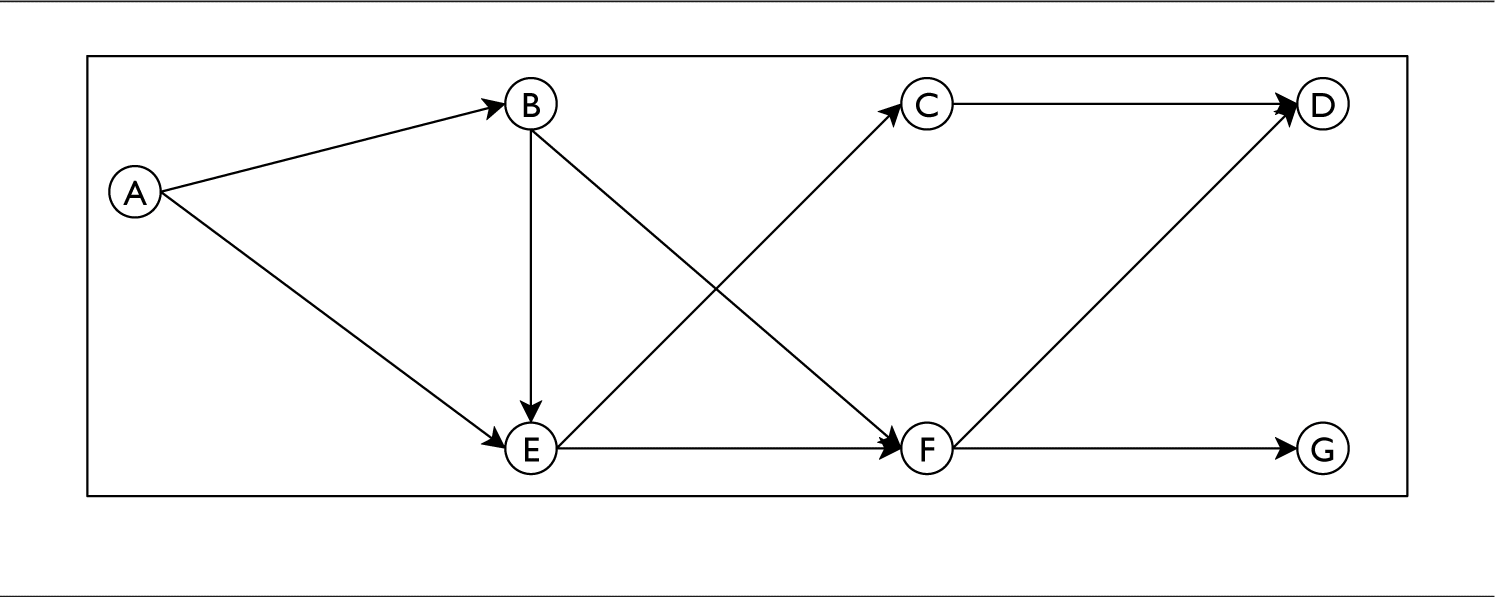
\includegraphics[width=0.75\textwidth]{images/00669.png}
  \caption{一个包含 7 个节点的小型有向图}
  \label{fig:sample-graph}
\end{figure}

形式化地，图由节点集合与连接节点的边集合构成。在有向图中，边代表单向关联；而在无向图中，边代表双向连通。在此背景下，如下是一个极具现实意义的典型问题：

\begin{notebox}[样例问题]
在某大型公司的内部邮件网络（有向图）中，设计一个算法为某员工规划向另一陌生员工递进引荐的联络路线。程序接收表示已建邮件通信的有向图以及两个邮箱节点，返回从起点连接到终点的一系列中间人邮箱序列。
\end{notebox}

数学家将这种从起点到终点的连通序列称为\term{路径（path）}。

图~\ref{fig:sample-graph} 将该问题具象化。例如，寻找从节点 \code{C} 到 \code{D} 的路径，该路径由起点 \code{C} 和终点 \code{D} 直接构成。而若要从 \code{E} 走到 \code{D}，则存在两条可选路径：
\begin{itemize}
  \item 从 \code{E} 经由 \code{F} 走向 \code{D}；
  \item 从 \code{E} 经由 \code{C} 走向 \code{D}。
\end{itemize}
有时两个节点之间可能根本不存在有效路径。例如在图~\ref{fig:sample-graph} 中，顺着箭头的方向无论如何也无法从 \code{C} 抵达 \code{G}。

如果将该有向图想象成一座大公园，你要从 \code{E} 走到 \code{G}：从 \code{E} 出发有两条岔路，一条通往 \code{C}，另一条通往 \code{F}。假定你先尝试第一条路走向 \code{C}，同时在脑海中记下“以后还可以尝试通往 \code{F} 的路线”。此时你面临一个全新问题：如何从 \code{C} 走到 \code{G}？这与原问题结构完全同构。然而从 \code{C} 出发无法到达 \code{G}，你陷入了死胡同。幸好，你记住了当初在 \code{E} 处还有另一条未走的选择，于是你\textbf{回溯}到 \code{E}，改走通往 \code{F} 的分支，最终顺利抵达目的地 \code{G}。

遵循设计配方，首先建立图的数据表示。图~\ref{fig:sample-graph} 可以表示为邻接表：
\begin{lstlisting}[language=BSL]
; Node 是 Symbol
; Graph 是 [List-of (list Node [List-of Node])]
; 或者 [List-of (cons Node [List-of Node])]

(define sample-graph
  '((A (B E))
    (B (E F))
    (C (D))
    (D ())
    (E (C F))
    (F (D G))
    (G ())))
\end{lstlisting}

\begin{exercise}{邻接表与 neighbors 函数设计}{471}\label{ex:471}
依据上述数据表示，设计函数 \code{neighbors}。它接收节点 \code{n} 与有向图 \code{g}，输出 \code{n} 在 \code{g} 中的直接后继邻居节点列表。
\end{exercise}

定义路径查找函数 \code{find-path} 的签名与目的说明：
\begin{lstlisting}[language=BSL]
; Node Node Graph -> [Maybe Path]
; 在有向图 G 中寻找一条从 origination 到 destination 的路径
; 若不存在连通路径，则返回 #false
(define (find-path origination destination G)
  #false)
\end{lstlisting}

回答生成型递归的四个设计问题：
\begin{enumerate}
  \item \textbf{平凡情形判断}：当起点与终点恰好是同一个节点时（\code{(symbol=? origination destination)}），问题平凡解决。
  \item \textbf{平凡解}：路径只包含该单一节点 \code{(list destination)}。
  \item \textbf{生成子问题}：若起点与终点不同，必须考察起点的所有直接邻居节点 \code{next = (neighbors origination G)}。遍历这些邻居并逐一递归探索从邻居到终点的路径。由于邻居是一个列表，我们提出一个辅助函数愿望清单：\code{find-path/list}。
  \item \textbf{合并子问题的解}：若在某个邻居节点上成功找到了通往终点的候选路径 \code{candidate}，只需将当前的 \code{origination} 节点拼装到该候选路径的最前端（\code{(cons origination candidate)}）即可构成完整路径；若所有邻居分支皆告失败，则返回 \code{\#false}。
\end{enumerate}

图~\ref{fig:find-path-code} 呈现了 \code{find-path} 与相互递归辅助函数 \code{find-path/list} 的完整定义。注意 \code{find-path/list} 对邻居列表采用结构型递归：对首个邻居调用 \code{find-path}，若返回的是非布尔路径则直接返回；否则，\textbf{回溯}探索剩余的邻居分支。

\begin{figure}[htbp]
  \centering
\begin{lstlisting}[language=BSL]
; Node Node Graph -> [Maybe Path]
; 寻找从 origination 到 destination 的路径，失败返回 #false
(define (find-path origination destination G)
  (cond
    [(symbol=? origination destination) (list destination)]
    [else (local ((define next (neighbors origination G))
                  (define candidate
                    (find-path/list next destination G)))
            (cond
              [(boolean? candidate) #false]
              [else (cons origination candidate)]))]))

; [List-of Node] Node Graph -> [Maybe Path]
; 从邻居列表 lo-Os 中寻找一条到达 D 的路径；若无路径则返回 #false
(define (find-path/list lo-Os D G)
  (cond
    [(empty? lo-Os) #false]
    [else (local ((define candidate
                    (find-path (first lo-Os) D G)))
            (cond
              [(boolean? candidate)
               (find-path/list (rest lo-Os) D G)]
              [else candidate]))]))
\end{lstlisting}
  \caption{图中的路径查找与回溯算法}
  \label{fig:find-path-code}
\end{figure}

\begin{exercise}{测试 find-path 与全节点连通测试}{472}\label{ex:472}
测试 \code{find-path}：使用它寻找 \code{'A} 到 \code{'G} 的路径。它找到的是哪一条路径？为什么？
设计函数 \code{test-on-all-nodes}，接收图 \code{g}，判定是否在任意节点对之间均能正确返回路径或 \code{\#false}。
\end{exercise}

现在考察算法的停机性。在无环图（DAG）中，由于节点总数有限且无环路折返，\code{find-path} 必然停机。然而，若图中存在\term{环路（cycle）}，情况便急转直下。考察图~\ref{fig:cyclic-graph}：相比图~\ref{fig:sample-graph}，它仅增加了一条从 \code{C} 指向 \code{B} 的反向边。

\begin{figure}[htbp]
  \centering
  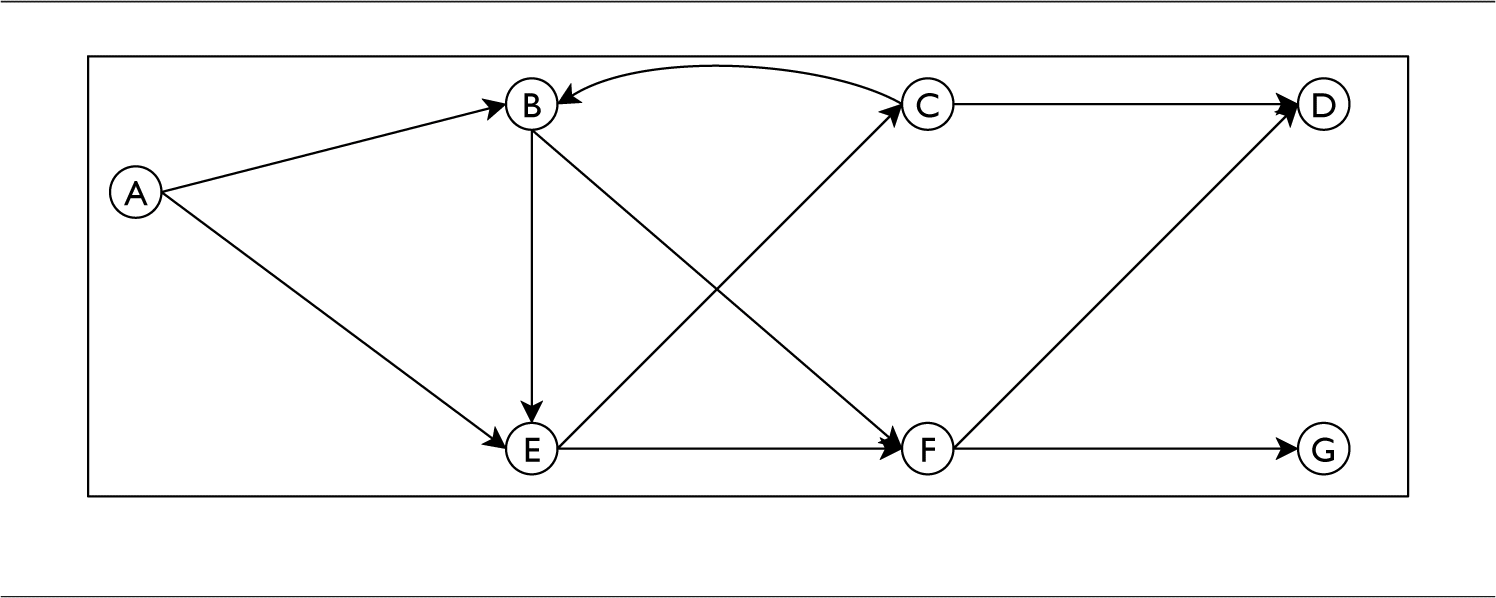
\includegraphics[width=0.75\textwidth]{images/00675.png}
  \caption{包含环路的有向图}
  \label{fig:cyclic-graph}
\end{figure}

如果在此有环图上执行 \code{(find-path 'B 'D cyclic-graph)}，算法将沿着 $B \to E \to C \to B$ 不断循环转圈，陷入死循环！
手工推导表明：在 7 步相互递归调用后，求值环境再次面临完全相同的表达式 \code{(find-path 'B 'D cyclic-graph)}。由于缺乏已访问节点的记忆机制，函数在此类有环图上无法停机。在第 VI 部分中，我们将借助“累加器”记录访问历史来彻底攻克这一难题。

\begin{exercise}{环路图上的行为测试}{473}\label{ex:473}
在图~\ref{fig:cyclic-graph} 所示的有环图上测试 \code{find-path 'B 'C cyclic-graph}，观察 DrRacket 的执行表现。
\end{exercise}

\begin{exercise}{单函数重构 find-path}{474}\label{ex:474}
使用 \code{local} 表达式将 \code{find-path} 与 \code{find-path/list} 整合重构为一个单一的顶级函数。
\end{exercise}

\begin{exercise}{使用 ormap 重构 find-path/list}{475}\label{ex:475}
能否利用列表抽象函数（如标准库中的高阶函数）来消除显式的结构型递归？探索 Racket 的 \code{ormap} 与 ISL+ 的不同之处，评估其在此处的适用性。
\end{exercise}

\begin{exercise}{有限状态自动机字符匹配 fsm-match?}{476}\label{ex:476}
设计函数 \code{fsm-match?}。它接收有限状态自动机（FSM）的数据表示与字符串，判断该字符串是否能驱动该自动机从初始状态转移并最终停留在接受状态。
提示：在 \code{local} 中定义辅助函数，将计算状态表示为当前状态与剩余字符列表的二元对。
\end{exercise}

\begin{figure}[htbp]
  \centering
\begin{lstlisting}[language=BSL]
; [List-of X] -> [List-of [List-of X]]
; 生成列表 w 中所有元素的全排列列表
(define (arrangements w)
  (cond
    [(empty? w) '(())]
    [else
     (foldr (lambda (item others)
              (local ((define without-item
                        (arrangements (remove item w)))
                      (define add-item-to-front
                        (map (lambda (a) (cons item a))
                             without-item)))
                (append add-item-to-front others)))
            '()
            w)]))
\end{lstlisting}
  \caption{基于生成型递归与列表抽象的全排列算法}
  \label{fig:arrangements-code}
\end{figure}

\begin{exercise}{基于生成型递归的排列全排列 arrangements}{477}\label{ex:477}
图~\ref{fig:arrangements-code} 展示了通过生成型递归与 \code{foldr}、\code{map} 组合实现的全排列生成函数 \code{arrangements}。
阐明其算法设计逻辑，回答生成型递归的全部核心问题，并为其撰写终止性论证。该实现生成的排列列表与第 12.4 节中的顺序是否完全一致？
\end{exercise}

\section{综合项目：N 皇后谜题}
\label{sec:29_2}

国际象棋中的\term{$N$ 皇后谜题（$n$ queens puzzle）}是展示回溯算法魅力的极佳典范。一个标准国际象棋棋盘由 $n \times n$ 个方格组成。皇后可以沿水平、垂直或对角线方向移动任意距离（如图~\ref{fig:queen-threat} 所示）。若某方格处于皇后的行进路线上，称该方格受到该皇后的\term{攻击威胁（threatened）}。

\begin{figure}[htbp]
  \centering
  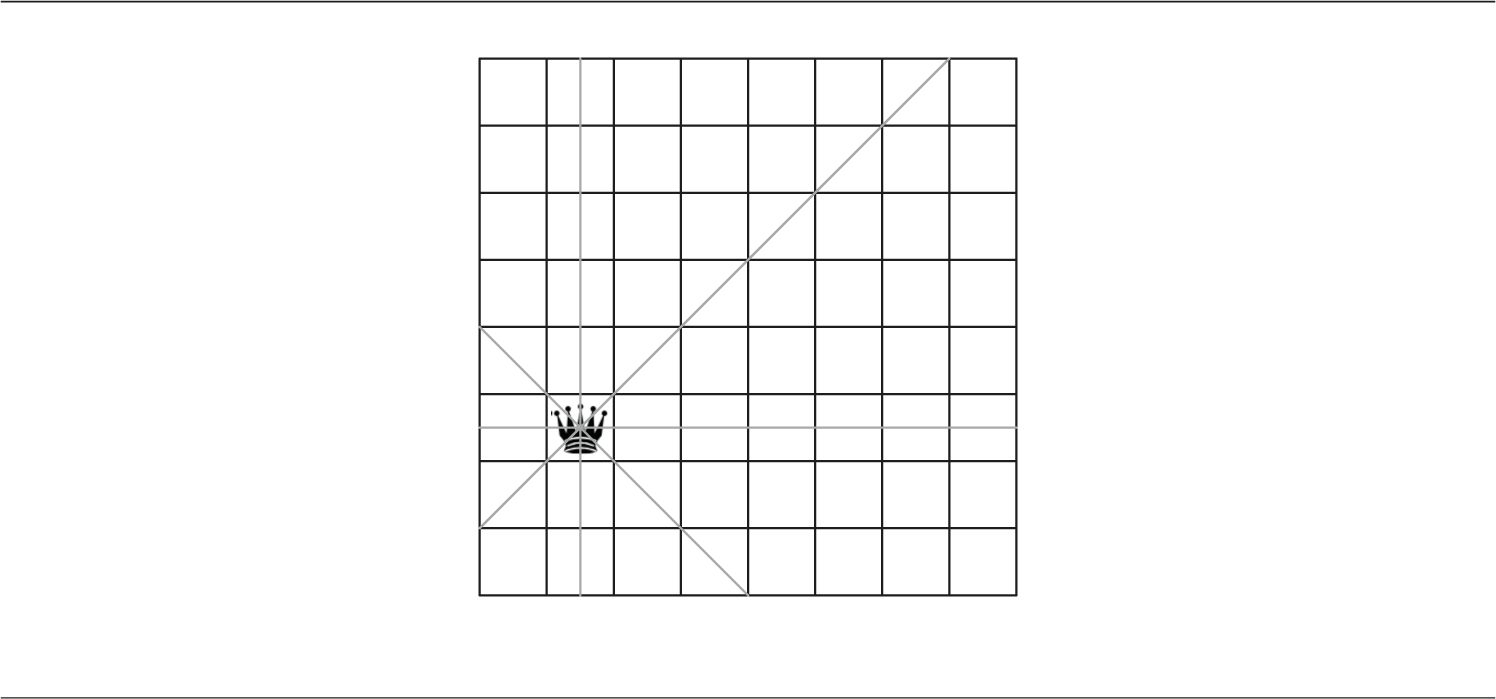
\includegraphics[width=0.65\textwidth]{images/00678.jpeg}
  \caption{棋盘上的单个皇后及其辐射威胁范围}
  \label{fig:queen-threat}
\end{figure}

经典 8 皇后问题要求在 $8 \times 8$ 棋盘上放置 8 个皇后，使得彼此互不受攻击。计算机科学家将其推广为任意规模的 $n$ 皇后谜题。显然，当 $n = 2$ 或 $n = 3$ 时，谜题无解（如图~\ref{fig:queens-3x3} 所示，放置两个互不攻击的皇后后，棋盘已无任何安全空格可供第三个皇后安放）。图~\ref{fig:queens-solutions} 给出了 $n=4$ 与 $n=5$ 的可行解。

\begin{figure}[htbp]
  \centering
  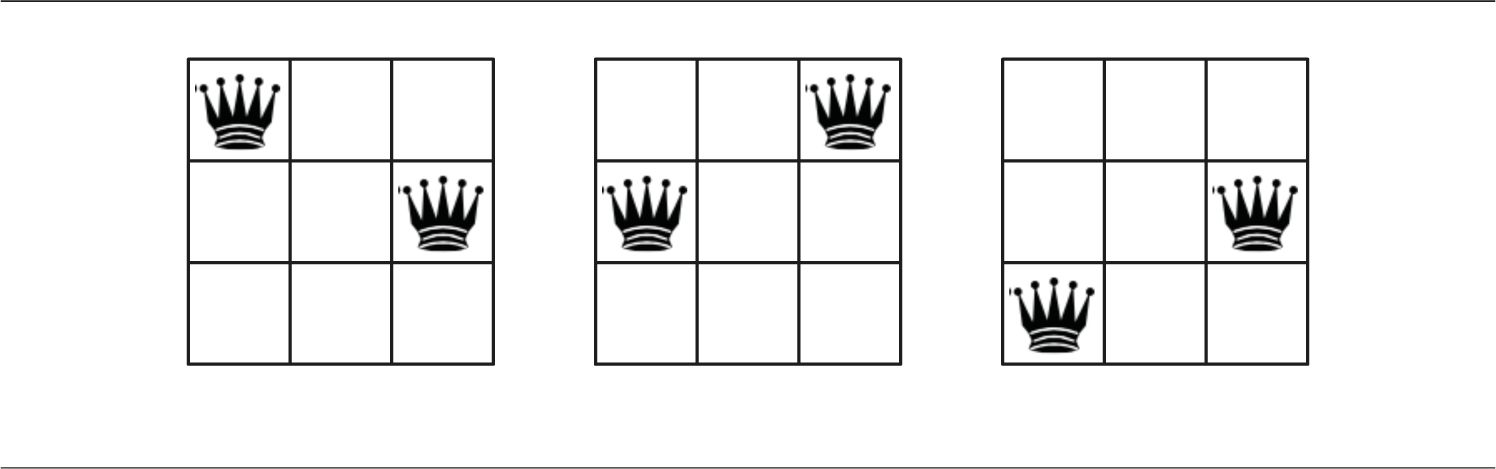
\includegraphics[width=0.75\textwidth]{images/00679.jpeg}
  \caption{$3 \times 3$ 棋盘上放置两个皇后的所有尝试均导致剩余方格全受威胁}
  \label{fig:queens-3x3}
\end{figure}

\begin{figure}[htbp]
  \centering
  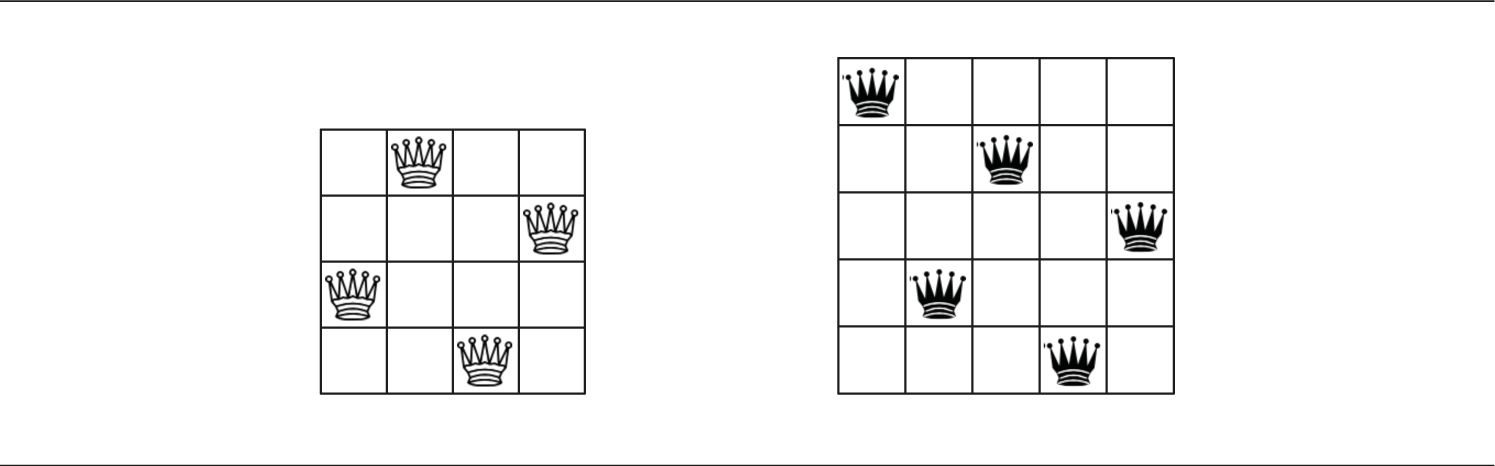
\includegraphics[width=0.85\textwidth]{images/00680.jpeg}
  \caption{$4 \times 4$ 与 $5 \times 5$ 棋盘的 $N$ 皇后合法解}
  \label{fig:queens-solutions}
\end{figure}

求解 $N$ 皇后问题的回溯思维如下：
\begin{enumerate}
  \item 一次放置一个皇后。放置后，标记其辐射的所有行、列与对角线为不可用；
  \item 对于下一个皇后，仅考虑尚未受到威胁的安全空位；
  \item 记录当前步骤的所有可选安全格；
  \item 若在某一阶段需要放置皇后却无任何安全空格可用，则说明先前的选择有误，立即\textbf{回溯}到上一步，改选上一步的下一个备选空格继续尝试。
\end{enumerate}

棋盘位置的数据表示：
\begin{lstlisting}[language=BSL]
(define QUEENS 8)

; QP 是结构体：(make-posn CI CI)
; CI 是区间 [0, QUEENS) 内的自然数
; 解释：(make-posn r c) 表示位于第 r 行第 c 列的方格
\end{lstlisting}

\begin{exercise}{威胁判断函数 threatening?}{479}\label{ex:479}
设计函数 \code{threatening?}。它接收两个 \code{QP} 位置，判定放置在两处的皇后是否会相互威胁。
数学洞见：
\begin{itemize}
  \item 水平威胁：行坐标相等（$r_1 = r_2$）；
  \item 垂直威胁：列坐标相等（$c_1 = c_2$）；
  \item 45 度对角线威胁：坐标和相等（$r_1 + c_1 = r_2 + c_2$）；
  \item 135 度对角线威胁：坐标差绝对值相等（$|r_1 - c_1| = |r_2 - c_2|$）。
\end{itemize}
\end{exercise}

\begin{exercise}{棋盘与皇后的图形化绘制 render-queens}{480}\label{ex:480}
设计函数 \code{render-queens}。接收自然数 $n$、皇后位置列表 \code{[List-of QP]} 以及棋子图像，绘制带有皇后的 $n \times n$ 棋盘。
\end{exercise}

算法主体 \code{n-queens} 的顶层定义如图~\ref{fig:n-queens-code} 所示。它将任务委托给辅助回溯函数 \code{place-queens}。

\begin{figure}[htbp]
  \centering
\begin{lstlisting}[language=BSL]
; N -> [Maybe [List-of QP]]
; 求解 n 皇后问题，成功返回皇后坐标列表，无解返回 #false

(define (n-queens n)
  (place-queens (board0 n) n))
\end{lstlisting}
  \caption{$N$ 皇后主求解函数}
  \label{fig:n-queens-code}
\end{figure}

\begin{exercise}{解的性质验证与集合等价谓词}{481}\label{ex:481}
设计高阶谓词 \code{n-queens-solution?}：接收 $n$，生成用于检验候选位置列表是否为有效 $n$ 皇后解的谓词（长度为 $n$ 且任意两两互不威胁）。
设计集合等价函数 \code{set=?}，判定两个列表在忽略元素次序的前提下是否包含完全相同的元素。
\end{exercise}

\begin{exercise}{核心放置算法 place-queens}{482}\label{ex:482}
依据回溯策略设计 \code{place-queens}：
\begin{lstlisting}[language=BSL]
; Board N -> [Maybe [List-of QP]]
; 在已有棋盘 a-board 上放置剩余的 n 个皇后；若无解返回 #false
(define (place-queens a-board n)
  #false)
\end{lstlisting}
假设针对棋盘抽象数据类型已拥有如下愿望清单函数：
\begin{itemize}
  \item \code{board0}：创建初始的空棋盘；
  \item \code{add-queen}：在棋盘的指定位置放置皇后并更新受威胁状态；
  \item \code{find-open-spots}：返回当前棋盘上所有依然安全的开阔空位列表。
\end{itemize}
\end{exercise}

\begin{exercise}{棋盘的三种数据表示与数据抽象}{483}\label{ex:483}
为 \code{Board} 设计具体的数据表示并实现练习~\ref{ex:482} 中的愿望清单函数。考虑以下三种不同建模思路：
\begin{enumerate}
  \item 棋盘表示为当前所有\textbf{仍可放置皇后的安全方格}列表；
  \item 棋盘表示为\textbf{已放置的所有皇后位置}列表；
  \item 棋盘表示为一个包含 $n \times n$ 个方格结构体的网格列表，每个格子记录自身坐标及是否受威胁的状态。
\end{enumerate}
体会数据抽象的威力：只要底层接口保持一致，算法核心代码无需做任何修改即可无缝运行！
\end{exercise}

% ==============================================================================
% 第 30 章：总结 (Chapter 30: Summary)
% ==============================================================================

\chapter{总结}
\label{sec:ch30_summary}

本书第五部分将“顿悟”（Eureka!）的灵感引入了程序设计。与前四部分严格遵循数据定义的结构化设计不同，灵感设计始于对程序应\textbf{如何解决问题}或\textbf{如何处理表征问题的数据}的算法巧思。在这一语境下，设计意味着构想出一种精妙机制：在与原问题性质相同但规模更简单的新子问题上发起递归调用。

请牢记：尽管我们将其学术性地命名为\term{生成型递归（generative recursion）}，但绝大多数计算机科学家与软件工程师通常直接将此类函数称为\term{算法（algorithms）}。

学完本书的这一部分之后，你应该对生成型递归的设计建立起如下深刻理解：

\begin{enumerate}
  \item \textbf{设计配方的大体框架依然坚挺有效}：问题分析、数据定义、签名、目的说明、示例用例与测试步骤一如既往地规范着我们的思维路线。
  \item \textbf{主要变革发生于从模板到编码的实现步骤}：通用算法蓝图引出了关于如何具体实现函数的\textbf{四个核心问题}。其中前两个问题用于确立并解决“平凡”（trivial）边界情形，而后两个问题则用于规划新子问题的生成策略以及子问题之解的拼装合并。
  \item \textbf{关键的增补在于终止性分析}：与天然保证终止的结构型递归函数不同，算法在某些特定输入下可能无法停机。这种非终止现象可能源于算法思想本身的理论局限性，也可能源于从数学到代码实现过程中的离散化缺陷（如除零、浮点溢出或图环路死循环）。无论何种情况，未来的代码读者与维护者都理应在目的说明中获得关于潜在异常输入的清晰警示。
\end{enumerate}

在真实的职业编程生涯中，你会频繁遇到一些简单或经典的现成算法，并被期望能够轻车熟路地将其落地实现。而对于那些真正极其复杂精妙的尖端算法，顶尖科技公司通常会聘请高薪专家、领域学者和数学家在白板上推导完所有数学细节后，再交由程序员将其转化为高效软件系统。你也必须为此类高难度协作做好充分准备，而通往卓越的最佳途径唯有躬行实践。

% ==============================================================================
% 插曲 5：计算开销 (Intermezzo 5: The Cost of Computation)
% ==============================================================================

\intermezzo{插曲 5：计算开销}
\label{sec:intermezzo05}

当程序 $f$ 顺利通过以下三项测试时，你能断言关于 $f$ 的哪些性质？

\begin{lstlisting}[language=BSL]
(check-expect (f 0) 0)
(check-expect (f 1) 1)
(check-expect (f 2) 8)
\end{lstlisting}

如果这道题出现在标准测试卷中，你可能会自然写出立方函数：
\begin{lstlisting}[language=BSL]
(define (f x) (expt x 3))
\end{lstlisting}
但事实上，没有任何理由能排除如下定义：
\begin{lstlisting}[language=BSL]
(define (f x) (if (= x 2) 8 (* x x)))
\end{lstlisting}
测试仅仅表明：程序在\textbf{某些特定输入}上的行为符合预期，仅此而已。

同理，对特定输入测试程序的求值耗时，仅仅告诉你针对这些孤立输入的执行时间——它无法外推到未知规模的输入。设想你有两个程序：\code{prog-linear} 与 \code{prog-square}，它们在给定相同输入时总是产生相同的答案，且在你随手挑选的若干测试样本上，\code{prog-linear} 总是比 \code{prog-square} 更快。第 26.4 节便展示了这样一对程序：结构型递归的 \code{gcd-structural} 与生成型递归的 \code{gcd-generative}，后者实测耗时远短于前者。

你有多大把握能断言 \code{prog-linear} 在任何情况下都优于 \code{prog-square}？考察图~\ref{fig:runtime-crossover} 中的函数曲线图。横轴表示输入规模（例如列表的长度 $n$），纵轴表示计算耗时。直线代表 \code{prog-linear} 的耗时，而抛物曲线代表 \code{prog-square} 的耗时。在阴影区域内，由于常数因子的影响，\code{prog-linear} 的耗时反而高于 \code{prog-square}；直到跨过交叉点阈值之后，\code{prog-square} 的耗时才发生剧烈陡增并远超 \code{prog-linear}。如果你仅仅在阴影区域的小规模输入上测试性能，而用户实际运行的数据却大量处于非阴影的大规模区域，你就会向用户交付一个错误且低效的程序。

\begin{figure}[htbp]
  \centering
  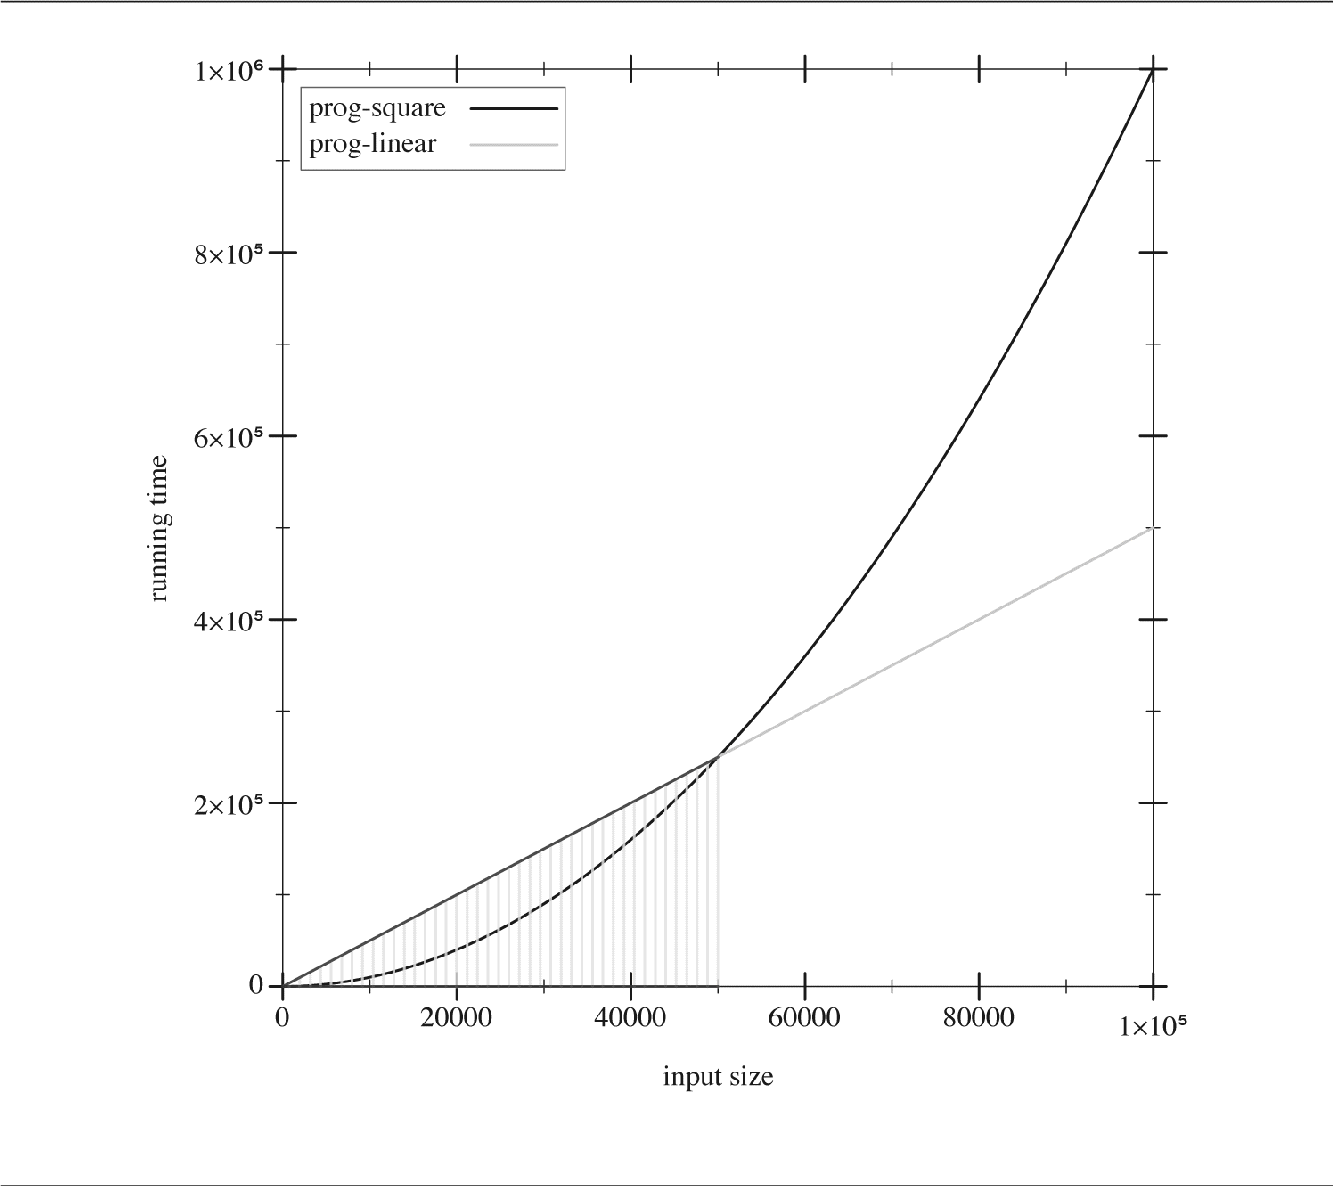
\includegraphics[width=0.75\textwidth]{images/00685.png}
  \caption{两种运行时间表达式的增长对比与交叉平衡点}
  \label{fig:runtime-crossover}
\end{figure}

本插曲正式引入\term{算法分析（algorithmic analysis）}的核心思想。它使程序员能够超越机器与环境的偶然干扰，对程序的性能本质做出普遍性陈述。任何严谨的计算机科学家与软件工程师都必须彻底精通这一概念。

\intermezzosection{具体时间与抽象时间}

第 26.4 节指出，\code{gcd-generative} 之所以从根本上优于 \code{gcd-structural}，是因为前者求解时所需的\textbf{递归步骤总数}远少于后者。以此为起点，我们来分析第 9 章中计算列表长度的简单程序 \code{how-many}：

\begin{lstlisting}[language=BSL]
(define (how-many a-list)
  (cond
    [(empty? a-list) 0]
    [else (+ (how-many (rest a-list)) 1)]))
\end{lstlisting}

利用插曲 1 中的代数代换规则，观察其在非空列表上的单步演算：
\begin{lstlisting}[language=BSL]
  (how-many some-non-empty-list)
== (cond
     [(empty? some-non-empty-list) 0]
     [else (+ (how-many (rest some-non-empty-list)) 1)])
== (cond
     [#false 0]
     [else (+ (how-many (rest some-non-empty-list)) 1)])
== (+ (how-many (rest some-non-empty-list)) 1)
\end{lstlisting}

在现代计算机体系中，判断列表构造器类型（\code{empty?}）、检查 \code{cond} 分支以及提取子结构（\code{rest}）所耗费的时间都是极其微小且恒定的常数。因此，\code{(how-many a-list)} 的总计算耗时，本质上正比于递归调用的总次数——对于长度为 $n$ 的列表，程序精确执行 $n$ 次递归展开。

这种抽象抽离了硬件时钟频率、编译器优化等底层偶然细节，将性能刻画为\textbf{输入规模 $n$ 与所需基本操作（递归步数）之间的函数关系}。计算机科学家称之为程序的\term{抽象运行时间（abstract running time）}。

对于 \code{how-many}，我们说它的计算时间“与输入规模 $n$ 处于同一数量级”（on the order of $n$ steps）。

并非所有程序的求值步数都像 \code{how-many} 那样固定。考察检索列表中是否包含特定符号的函数：
\begin{lstlisting}[language=BSL]
(define (contains-flatt? lo-names)
  (cond
    [(empty? lo-names) #false]
    [(cons? lo-names)
     (or (symbol=? (first lo-names) 'flatt)
         (contains-flatt? (rest lo-names)))]))
\end{lstlisting}

若目标元素恰好位于列表首位，只需 0 次递归即可立即返回；而若目标元素位于列表末尾或根本不存在，则必须完整遍历所有 $n$ 个元素。这一差异引出了算法分析的三种核心视角：
\begin{itemize}
  \item \textbf{最好情况分析（Best-case analysis）}：针对最有利于程序的输入形态评估性能（例如首元素即为目标，耗时为常数步）。
  \item \textbf{最坏情况分析（Worst-case analysis）}：针对最苛刻极端、最耗时的输入评估性能瓶颈（例如目标位于末尾，需遍历 $n$ 步）。
  \item \textbf{平均情况分析（Average-case analysis）}：假设输入数据随机均匀分布，评估平均期望耗时（例如平均在中间位置找到目标，需 $n/2$ 步）。
\end{itemize}

在抽象分析中，常数因子（如 $n/2$ 中的系数 $1/2$）可以被忽略。设每步基本操作耗时为常数 $k$，换用两倍主频的新 CPU 后耗时减半为 $k/2$；但无论系数常数如何变化，增长的几何本质始终是 $n$ 的线性函数。

现在考察插入排序算法（第 11 章）。对其进行手工推演：
\begin{lstlisting}[language=BSL]
  (sort (list 3 1 2))
== (insert 3 (sort (list 1 2)))
== (insert 3 (insert 1 (sort (list 2))))
== (insert 3 (insert 1 (insert 2 (sort '()))))
== (insert 3 (insert 1 (insert 2 '())))
== (insert 3 (insert 1 (list 2)))
== (insert 3 (list 2 1))
== (list 3 2 1)
\end{lstlisting}

\code{sort} 首先递归展开 $n$ 次，随后触发 $n$ 次 \code{insert} 插入操作。每次将元素插入到长度为 $l$ 的有序列表时，平均需要比较 $l/2$ 次。对于长度为 $n$ 的列表，插入操作的平均总步数为：
\[ \sum_{i=1}^{n-1} \frac{i}{2} = \frac{1}{2} \cdot \frac{n(n-1)}{2} = \frac{1}{4} n^2 - \frac{1}{4} n \]
当 $n$ 增长时，$n^2$ 项起决定性支配作用。因此，插入排序算法的耗时“与 $n^2$ 处于同一数量级”。

最后考察第 16.2 节中寻找列表最小值的朴素实现 \code{inf}：
\begin{lstlisting}[language=BSL]
(define (inf l)
  (cond
    [(empty? (rest l)) (first l)]
    [else (if (< (first l) (inf (rest l)))
              (first l)
              (inf (rest l)))]))
\end{lstlisting}
当列表按降序排列时（最坏情况），\code{if} 的判断条件为假，程序被迫在 \code{else} 分支中再次对 \code{(rest l)} 重新完整执行一次递归调用！对于包含 4 个元素的列表，需要执行 8 次调用；每增加一个元素，调用树的分支数直接翻倍。其总递归步数为 $2^{n-1}$，属于灾难性的\textbf{指数级复杂度}（$O(2^n)$）。

\begin{exercise}{局部变量优化 infL 的复杂度分析}{484}\label{ex:484}
回顾利用 \code{local} 避免重复计算的改进版本 \code{infL}：
\begin{lstlisting}[language=BSL]
(define (infL l)
  (cond
    [(empty? (rest l)) (first l)]
    [else (local ((define s (infL (rest l))))
            (if (< (first l) s) (first l) s))]))
\end{lstlisting}
推导对 \code{(list 3 2 1 0)} 的求值过程。论证在最好与最坏情况下，\code{infL} 的步数均已降为 $n$ 数量级。
\end{exercise}

\begin{exercise}{数字二叉树求和 sum-tree}{485}\label{ex:485}
数字树（Number Tree）要么是一个数字，要么是一对数字树构成的有序对。设计函数 \code{sum-tree} 计算树中所有数字的总和。
分析其抽象运行时间：如何合理定义一棵树的“规模”？在相同规模下，何种树形对应最坏情况？何种对应最好情况？
\end{exercise}

\intermezzosection{“大 $O$ 记号”的形式化定义}

计算机科学使用严格的数学语言——\term{大 $O$ 记号（Big-O notation）}来标准化上述关于增长数量级的讨论。

\begin{notebox}[大 $O$ 记号定义]
设 $g(n)$ 是定义在自然数集合上的函数。记号 $\mathcal{O}(g)$（读作“$g$ 的大 $O$”）表示一类函数集合。若存在正实数 $c$ 与正整数 $n_0$（即 \code{bigEnough}），使得对于所有满足 $n \ge n_0$ 的自变量 $n$，不等式恒成立：
\[ f(n) \le c \cdot g(n) \]
则称函数 $f$ 属于 $\mathcal{O}(g)$，记作 $f \in \mathcal{O}(g)$（或通俗写作 $f(n) = \mathcal{O}(g(n))$）。

\textbf{术语含义}：若 $f \in \mathcal{O}(g)$，则表明当问题规模充分大时，$f$ 的增长速度\textbf{绝不差于（不超过）} $g$ 的常数倍。
\end{notebox}

以前文提到的线性程序与平方程序为例：
\[ H(n) = 1000n, \quad G(n) = n^2 \]
选取常数 $c = 1$ 与 $n_0 = 1000$。对于任意 $n \ge 1000$，两边同乘正数 $n$ 即得：
\[ 1000n \le n^2 \implies H(n) \le 1 \cdot G(n) \]
由此在数学上严格证明了 $H \in \mathcal{O}(G)$，即线性程序从渐进意义上绝不慢于平方程序。

在大 $O$ 分析中，低阶项与常数因子均被舍弃：
\begin{itemize}
  \item $\mathcal{O}(1)$：常数复杂度，操作耗时与输入规模完全无关；
  \item $\mathcal{O}(n)$：线性复杂度，耗时与输入规模成正比；
  \item $\mathcal{O}(n \log n)$：线性对数复杂度，如快速排序的平均性能；
  \item $\mathcal{O}(n^2)$：平方复杂度，如冒泡排序、插入排序；
  \item $\mathcal{O}(2^n)$：指数复杂度，通常意味着算法对于中大规模输入完全不可用。
\end{itemize}

\begin{exercise}{证明多项式属于 O(n\textasciicircum 2)}{486}\label{ex:486}
证明函数 $f(n) = n^2 + n$ 属于 $\mathcal{O}(n^2)$。明确给出一组满足定义的常数对 $(c, n_0)$。
\end{exercise}

\begin{exercise}{指数爆炸与常数倍线性对比}{487}\label{ex:487}
考察函数 $f(n) = 2^n$ 与 $g(n) = 1000n$。证明 $g \in \mathcal{O}(f)$。如果已知现实应用中输入规模严格处于 $[3, 12]$ 之间，哪一个算法在实践中表现更优？
\end{exercise}

\begin{exercise}{对数线性与平方对比}{488}\label{ex:488}
对比函数 $f(n) = n \log_2(n)$ 与 $g(n) = n^2$。是 $f \in \mathcal{O}(g)$ 成立，还是 $g \in \mathcal{O}(f)$ 成立？写出推导依据。
\end{exercise}

\intermezzosection{为何程序应当使用结构化谓词与选择器？}

大 $O$ 分析能够从计算复杂度的角度，有力证明为什么遵循设计配方能够产出既优雅又高效的高质量程序。

考虑在数字列表中检索目标数字的任务：
\begin{lstlisting}[language=BSL]
; Number [List-of Number] -> Boolean
; 判定 x 是否存在于列表 l 中
(check-expect (search 0 '(3 2 1 0)) #true)
(check-expect (search 4 '(3 2 1 0)) #false)
\end{lstlisting}

对比以下两种实现：

\begin{figure}[htbp]
  \centering
  \begin{minipage}{0.48\textwidth}
\begin{lstlisting}[language=BSL]
(define (searchL x l)
  (cond
    [(empty? l) #false]
    [else
     (or (= (first l) x)
         (searchL x (rest l)))]))
\end{lstlisting}
  \end{minipage}
  \hfill
  \begin{minipage}{0.48\textwidth}
\begin{lstlisting}[language=BSL]
(define (searchS x l)
  (cond
    [(= (length l) 0) #false]
    [else
     (or (= (first l) x)
         (searchS x (rest l)))]))
\end{lstlisting}
  \end{minipage}
  \caption{遵循结构化谓词的 \code{searchL} 与调用长度求值的 \code{searchS}}
  \label{fig:search-comparison}
\end{figure}

左侧的 \code{searchL} 严格遵循设计配方，采用基础结构化谓词 \code{empty?} 作为条件分支。每次检查耗费 $\mathcal{O}(1)$ 常数时间，对长度为 $n$ 的列表总复杂度为严格的 $\mathcal{O}(n)$。

右侧的 \code{searchS} 脱离了配方指导，采用“先求列表长度再判断是否为 0”的直觉思路。然而在链表模型中，\code{length} 本身是一个必须从头遍历整个列表的 $\mathcal{O}(l)$ 操作！在每一次递归调用中都调用一次 \code{length}，导致总运算步数退化为：
\[ \sum_{i=1}^n i = \frac{n(n+1)}{2} \implies \mathcal{O}(n^2) \]
仅仅因为改用了一个非结构化的外部操作，程序的复杂度便硬生生从线性级堕入平方级灾难！

编写如下性能测试函数并在 DrRacket 中亲自体会这一悬殊差距：
\begin{lstlisting}[language=BSL]
; N -> [List Number Number]
; 测量 searchS 与 searchL 在长度为 n 的列表上的实际耗时
(define (timing n)
  (local ((define long-list (build-list n (lambda (i) i))))
    (list
      (time (searchS n long-list))
      (time (searchL n long-list)))))
\end{lstlisting}

在交互区分别对 $n = 10000$ 与 $n = 20000$ 执行测试：\code{searchL} 的耗时仅随 $n$ 翻倍而平缓线性翻倍，而 \code{searchS} 的耗时将呈现 4 倍的爆发式暴涨！

这一鲜明实验告诫我们：在函数设计中，\textbf{严格遵循结构化设计配方与原生谓词选择器}，不仅保证了逻辑的严谨无瑕，更为算法的底层运行性能筑起了坚不可摧的基石。


% ==================== 第六部分：累加器 ====================
\part{累加器 (Accumulators)}
% ==============================================================================
% 第 31 章：上下文信息的丢失 (Chapter 31: The Loss of Knowledge)
% ==============================================================================

\chapter{上下文信息的丢失}
\label{sec:ch31_loss_of_knowledge}

无论依据结构化设计配方还是生成型递归设计配方设计的函数，都会面临\term{上下文信息的丢失}（loss of knowledge）这一问题，尽管在两类设计中其具体表现形式各不相同。本章通过两个典型示例——结构化与生成式各取其一——阐释缺乏上下文信息将如何对函数的运行性能乃至正确性产生负面影响。第 \ref{sec:ch31_1} 节探讨结构型递归中的上下文信息丢失问题，而第 \ref{sec:ch31_2} 节则深入剖析生成型递归场景下的同类关切。

\section{结构化处理中的问题}
\label{sec:ch31_1}

让我们从一个看似十分直观的示例出发：

\begin{notebox}[问题陈述：相对距离转绝对距离]
你正在为一个负责测量道路路段长度的测绘团队工作。该团队请你设计一个程序，将一条道路上一系列路点之间的\term{相对距离}（relative distances）转换为相对于某个起点的\term{绝对距离}（absolute distances）。
\end{notebox}

例如，假设给定一条带有测点的道路，其各段相对距离标示如下：

\begin{figure}[htbp]
  \centering
  \includegraphics[width=0.65\textwidth]{images/00713.png}
  \caption{路点之间的相对距离示意}
  \label{fig:relative_dist_sample}
\end{figure}

图中的每个数字表示两个相邻圆点之间的距离。而我们期望程序计算出的结果如下图所示，其中每个圆点都标注了它到最左端起点的绝对距离：

\begin{figure}[htbp]
  \centering
  \includegraphics[width=0.65\textwidth]{images/00714.png}
  \caption{各路点相对于起点的绝对距离示意}
  \label{fig:absolute_dist_sample}
\end{figure}

按照常规的结构化设计配方，设计一个完成此计算的程序只是一次标准的基础练习。图 \ref{fig:177} 给出了完整的程序实现。当输入的列表不为 \code{\textquotesingle()} 时，自然递归调用会计算出 \code{(rest l)} 中其余圆点相对于列表首个测点的绝对距离。然而，由于列表中第一个测点本身并不是绝对原点（它与真正原点的距离为 \code{(first l)}），我们必须将 \code{(first l)} 累加到自然递归计算出的列表中的每一项上。这第二步——将一个固定数值加到数字列表的每个元素上——需要一个辅助函数 \code{add-to-each}。

\begin{figure}[htbp]
  \centering
\begin{lstlisting}[language=BSL, basicstyle=\scriptsize\ttfamily]
; [List-of Number] -> [List-of Number]
; converts a list of relative to absolute distances
; the first number represents the distance to the origin

(check-expect (relative->absolute '(50 40 70 30 30))
              '(50 90 160 190 220))

(define (relative->absolute l)
  (cond
    [(empty? l) '()]
    [else (local ((define rest-of-l
                    (relative->absolute (rest l)))
                  (define adjusted
                    (add-to-each (first l) rest-of-l)))
            (cons (first l) adjusted))]))

; Number [List-of Number] -> [List-of Number]
; adds n to each number on l

(check-expect (cons 50 (add-to-each 50 '(40 110 140 170)))
              '(50 90 160 190 220))

(define (add-to-each n l)
  (cond
    [(empty? l) '()]
    [else (cons (+ (first l) n) (add-to-each n (rest l)))]))
\end{lstlisting}
  \caption{将相对距离转换为绝对距离（结构型递归版本）}
  \label{fig:177}
\end{figure}

虽然设计这个程序直截了当，但在越来越长的列表上运行它却暴露出一个严重问题。考虑对以下表达式的求值：

\begin{lstlisting}[language=BSL]
(relative->absolute (build-list size add1))
\end{lstlisting}

随着 \code{size} 的增加，程序运行所需的时间呈现出急剧加速的态势：

\begin{table}[htbp]
  \centering
  \caption{函数 \code{relative->absolute} 在不同规模列表上的运行耗时（毫秒）}
  \label{fig:rel_abs_perf_table}
  \small
  \setlength{\tabcolsep}{3.5pt}
  \begin{tabular}{lrrrrrrr}
    \hline
    \code{size} & 1000 & 2000 & 3000 & 4000 & 5000 & 6000 & 7000 \\
    \hline
    \code{time} & 25 & 109 & 234 & 429 & 689 & 978 & 1365 \\
    \hline
  \end{tabular}
\end{table}

当列表规模从 1000 翻倍至 2000 时，运行耗时并没有相应翻倍，而是膨胀到了原来的近 4 倍；从 2000 增长到 4000 同样保持了约 4 倍的增速。借用插曲 5 中的渐近复杂度术语，我们称该函数的运行时间性能为 $\mathcal{O}(n^2)$，其中 $n$ 代表输入列表的长度。

\begin{notebox}[关于测量耗时的说明]
不同计算机与不同测试年份的实际运行耗时会有所差异。上表中的测试数据于 2017 年在一台运行 OS X 10.11 的 MacMini 上实测获得；而该书第一版早先于 1998 年所作的测量耗时要高出大约 100 倍。
\end{notebox}

\begin{exercise}{重构辅助函数 add-to-each}{489}
使用抽象函数 \code{map} 与 \code{lambda} 表达式重新表述辅助函数 \code{add-to-each}。
\end{exercise}

\begin{exercise}{推导 relative->absolute 的抽象运行时间公式}{490}
推导出一个数学公式，用以描述函数 \code{relative->absolute} 的抽象运行时间。

\textbf{提示}：手工逐步推导求值表达式：
\begin{lstlisting}[language=BSL]
(relative->absolute (build-list size add1))
\end{lstlisting}
从将 \code{size} 分别替换为 1、2 和 3 开始。每次求值过程中，分别需要调用多少次 \code{relative->absolute} 与 \code{add-to-each} 的递归？
\end{exercise}

考虑到问题本身的简单性，该程序所执行的庞大计算量令人十分吃惊。如果由人工在草稿纸上进行同样的转换，我们通常会一边沿着直线前行，一边维护当前走过的累计总距离，并将新遇到的相对距离顺次叠加进去即可。为什么计算机程序不能像人一样这样工作呢？

让我们尝试设计一个更贴近人工心算方法的函数版本。我们依然从标准的列表处理模板出发：

\begin{lstlisting}[language=BSL]
(define (relative->absolute/a l)
  (cond
    [(empty? l) ...]
    [else
     (... (first l) ...
      ... (relative->absolute/a (rest l)) ...)]))
\end{lstlisting}

现在让我们模拟一次单步手工推导演算：

\begin{lstlisting}[language=BSL]
  (relative->absolute/a (list 3 2 7))
== (cons ... 3 ... (relative->absolute/a (list 2 7)))
== (cons ... 3 ...
     (cons ... 2 ...
       (relative->absolute/a (list 7))))
== (cons ... 3 ...
     (cons ... 2 ...
       (cons ... 7 ...
         (relative->absolute/a '()))))
\end{lstlisting}

结果列表的第一个元素显然应该是 3，构造它毫无困难。但是，第二个元素应该是 \code{(+ 3 2)} 即 5，而第 2 个 \code{relative->absolute/a} 递归实例却根本无法“获知”原始列表的第一个元素是 3。这里的“知识”在递归深入的过程中被丢失了！

根本原因在于：\term{递归函数在本质上是独立于其上下文的}（context-independent）。在 \code{(cons N L)} 中对 \code{L} 的处理方式，与在 \code{(cons K L)} 中对 \code{L} 的处理方式完全一致；即便单独把 \code{L} 传入函数，处理过程也毫无二致。

为了弥补这一“上下文信息的丢失”，我们为函数增设一个额外的参数：\code{accu-dist}。该参数代表\term{累积距离}（accumulated distance），即我们在遍历相对距离列表转换为绝对距离列表时所持续记录的累计账目。其初始值必然为 0。随着函数在列表中逐项前进，它必须将每个路点的相对距离叠加到这个累加账目上。

修改后的函数定义如下：

\begin{lstlisting}[language=BSL]
(define (relative->absolute/a l accu-dist)
  (cond
    [(empty? l) '()]
    [else
     (local ((define tally (+ (first l) accu-dist)))
       (cons tally
             (relative->absolute/a (rest l) tally)))]))
\end{lstlisting}

递归调用接收列表的余下部分 \code{(rest l)} 以及当前路点相对于原点的新绝对距离 \code{tally}。尽管每次递归调用中两个参数都会发生变化，但第二个参数的更新严格依赖于第一个参数。该函数依然是一个纯粹的结构化列表处理程序。

现在让我们再次对其进行手工求值演算：

\begin{lstlisting}[language=BSL]
   (relative->absolute/a (list 3 2 7) 0)
== (cons 3 (relative->absolute/a (list 2 7) 3))
== (cons 3 (cons 5 (relative->absolute/a (list 7) 5)))
== (cons 3 (cons 5 (cons 12 ???)))
== (cons 3 (cons 5 (cons 12 '())))
\end{lstlisting}

\begin{notebox}[请停下来思考！]
请自行补全第 4 行中的问号处内容：此时调用的参数是什么？
\end{notebox}

上述手工求值清晰地揭示了引入累加器后转换过程得到了多大幅度的简化。列表中的每个项仅被访问和处理一次。当 \code{relative->absolute/a} 到达参数列表的末尾时，整个结果已经完全构建完毕，不再需要任何后续的二次遍历加工。一般而言，对于包含 $n$ 个元素的列表，该函数仅需执行约 $n$ 步自然递归。

然而这也带来了一个接口上的问题：与原函数 \code{relative->absolute} 相比，新函数需要两个参数，而非一个。更严重的是，调用者可能会不小心错误调用 \code{relative->absolute/a}，给它传入一个非 0 的累加初始值。我们可以借助局部定义 \code{local} 来封装 \code{relative->absolute/a}，同时解决这两个问题。图 \ref{fig:178} 展示了最终的优雅设计。现在，就输入-输出行为而言，\code{relative->absolute.v2} 与原先的 \code{relative->absolute} 完全等价。

\begin{figure}[htbp]
  \centering
\begin{lstlisting}[language=BSL, basicstyle=\scriptsize\ttfamily]
; [List-of Number] -> [List-of Number]
; converts a list of relative to absolute distances
; the first number represents the distance to the origin

(check-expect (relative->absolute.v2 '(50 40 70 30 30))
              '(50 90 160 190 220))

(define (relative->absolute.v2 l0)
  (local (
    ; [List-of Number] Number -> [List-of Number]
    (define (relative->absolute/a l accu-dist)
      (cond
        [(empty? l) '()]
        [else
          (local ((define accu (+ (first l) accu-dist)))
            (cons accu
                  (relative->absolute/a (rest l) accu)))])))
    (relative->absolute/a l0 0)))
\end{lstlisting}
  \caption{使用累加器转换相对距离}
  \label{fig:178}
\end{figure}

现在让我们来看看新版本的实际运行性能。为此，我们对下列表达式进行求值测试：

\begin{lstlisting}[language=BSL]
(relative->absolute.v2 (build-list size add1))
\end{lstlisting}

并将不同规模下的测试结果列于下表：

\begin{table}[htbp]
  \centering
  \caption{累加器版本 \code{relative->absolute.v2} 的耗时对比（毫秒）}
  \label{fig:rel_abs_v2_perf_table}
  \small
  \setlength{\tabcolsep}{5pt}
  \begin{tabular}{lrrrrrrr}
    \hline
    \code{size} & 1000 & 2000 & 3000 & 4000 & 5000 & 6000 & 7000 \\
    \hline
    \code{time} & 0 & 0 & 0 & 0 & 0 & 1 & 1 \\
    \hline
  \end{tabular}
\end{table}

令人惊叹的是，即便是处理包含 7000 个数字的长列表，\code{relative->absolute.v2} 的耗时也始终在 1 毫秒上下！对比前后两个版本的性能表现，你可能会误以为累加器是治愈所有程序性能迟缓的灵丹妙药。遗憾的是现实并非总是如此，但\textbf{只要一个结构型递归函数必须对其自然递归返回的结果进行递归式的二次加工}，你就应当毫不犹豫地考虑使用累加器。在此特定案例中，程序的时间复杂度从 $\mathcal{O}(n^2)$ 骤降至 $\mathcal{O}(n)$，并且常数项系数也得到了大幅削减。

\begin{exercise}{通过列表抽象重构相对距离转换}{491}
本书第一版的一位读者通过巧妙的设计构思，给出了针对该问题如下简洁的解法：

\begin{lstlisting}[language=BSL]
(define (relative->absolute l)
  (reverse
    (foldr (lambda (f l) (cons (+ f (first l)) l))
           (list (first l))
           (reverse (rest l)))))
\end{lstlisting}

该方案仅使用了 ISL+ 中大家熟知的内置函数：\code{reverse} 与 \code{foldr}（使用 \code{lambda} 仅是为了书写便利）。读者可能还记得，在本书第三部分中，\code{foldr} 本身正是依据前两部分的设计配方完全可设计出来的。

你朋友的这种简短解法是否意味着本节引入的复杂累加器设计纯属多余？有关解答请参阅第 \ref{sec:ch32_1} 节，但在翻阅之前，请先深入反思这个问题。\textbf{提示}：尝试自行设计 \code{reverse} 函数并分析其性能开销。
\end{exercise}

\section{生成型递归中的问题}
\label{sec:ch31_2}

接下来让我们重温在图（Graph）中沿路径“漫游”的问题：

\begin{notebox}[问题陈述：简单图中的路径连通性判定]
设计一个算法，检查一个简单图中的两个节点之间是否存在连通路径。在所谓的简单图中，每个节点有且仅有一条指向另一个节点（或指向自身）的有向连接。
\end{notebox}

第 29 章讨论了算法必须找出具体路径的复杂场景。本节的问题要更简单，因为我们的核心目标在于探讨该算法的累加器版本设计。

考查图 \ref{fig:179} 所示的样例图。图中共有从 A 到 F 的 6 个节点和 6 条有向连接。从 A 到 E 的路径必定经过 B 和 C。然而，从 A 出发到 F 则不存在任何连通路径；除 F 本身之外，也没有任何其他节点能到达 F。

\begin{figure}[htbp]
  \centering
  \includegraphics[width=0.85\textwidth]{images/00723.png}
  \caption{一个简单图及其在 BSL 中的嵌套列表表示}
  \label{fig:179}
\end{figure}

图 \ref{fig:179} 的右半部分展示了如何使用嵌套列表在程序中表示此图。每个节点表示为一个包含两个符号的列表：第一个符号是该节点的标签，第二个符号则是从该节点出发单步可达的目标节点。相关的数据定义如下：

\begin{lstlisting}[language=BSL]
; A SimpleGraph is a [List-of Connection]
; A Connection is a list of two items:
;   (list Node Node)
; A Node is a Symbol.
\end{lstlisting}

这些数据定义是我们非形式化描述的自然转译。我们已经知道该问题需要运用生成型递归，其函数签名、目的说明与测试用例很容易编写：

\begin{lstlisting}[language=BSL]
; Node Node SimpleGraph -> Boolean
; 判断在简单图 sg 中是否存在从 origin 到 destination 的路径
(check-expect (path-exists? 'A 'E a-sg) #true)
(check-expect (path-exists? 'A 'F a-sg) #false)
(define (path-exists? origin destination sg)
  #false)
\end{lstlisting}

接下来我们需要回答生成型递归设计配方的四个核心问题：
\begin{enumerate}
  \item \textbf{问题在何种情况下是平凡可解的？} 当起点 \code{origin} 与终点 \code{destination} 完全相同时，问题平凡。
  \item \textbf{平凡解是什么？} 解为 \code{\#true}。
  \item \textbf{在非平凡情况下如何生成新问题？} 若起点与终点不同，我们唯一能做的就是迈向起点的直接邻居节点，并从该邻居节点出发继续搜寻目标终点。
  \item \textbf{如何组合子问题的解？} 如果新问题找到了解，无需做额外组合变换：只要起点的邻居能够到达终点，起点本身就能到达终点；否则说明不存在连通路径。
\end{enumerate}

将上述答案转译为 ISL+ 代码，便得到了图 \ref{fig:180} 所示的完整程序。其中包括用于在简单图中查找某节点邻居的辅助函数 \code{neighbor}（这只是一个结构型递归的基础练习），以及覆盖两种可能输出结果的测试用例。

\begin{figure}[htbp]
  \centering
\begin{lstlisting}[language=BSL, basicstyle=\scriptsize\ttfamily]
; Node Node SimpleGraph -> Boolean
; is there a path from origin to destination in sg

(check-expect (path-exists? 'A 'E a-sg) #true)
(check-expect (path-exists? 'A 'F a-sg) #false)

(define (path-exists? origin destination sg)
  (cond
    [(symbol=? origin destination) #t]
    [else (path-exists? (neighbor origin sg)
                        destination
                        sg)]))

; Node SimpleGraph -> Node
; determine the node that is connected to a-node in sg
(check-expect (neighbor 'A a-sg) 'B)
(check-error (neighbor 'G a-sg) "neighbor: not a node")
(define (neighbor a-node sg)
  (cond
    [(empty? sg) (error "neighbor: not a node")]
    [else (if (symbol=? (first (first sg)) a-node)
              (second (first sg))
              (neighbor a-node (rest sg)))]))
\end{lstlisting}
  \caption{在简单图中寻找路径（初始生成型递归版本）}
  \label{fig:180}
\end{figure}

\begin{notebox}[警告：请勿贸然运行该程序！]
请不要直接运行该程序。如果你运行了，请时刻准备好用鼠标点击 DrRacket 的“Stop”按钮以中止程序死循环。事实上，哪怕只是粗略审视一下该函数，就能发现隐藏的严重缺陷：尽管规范要求当两点间无路径时产生 \code{\#false}，但程序代码中压根就没有任何返回 \code{\#false} 的分支！反过来我们必须追问：当两个节点之间确实不存在连通路径时，这个函数究竟在做什么？
\end{notebox}

请再次观察图 \ref{fig:179}。在图中，从 C 到 D 显然不存在路径。从 C 出发连线直接越过 D 通向了 E。让我们对 \code{(path-exists? \textquotesingle C \textquotesingle D a-sg)} 做一次手工推导演算：

\begin{lstlisting}[language=BSL]
   (path-exists? 'C 'D '((A B) ... (F F)))
== (path-exists? 'E 'D '((A B) ... (F F)))
== (path-exists? 'B 'D '((A B) ... (F F)))
== (path-exists? 'C 'D '((A B) ... (F F)))
\end{lstlisting}

推导确凿地证实：随着函数的不断递归，它以\textbf{完全相同的参数组合}一次又一次地反复调用自身！换言之，求值陷入了永无止境的死循环中。

这里暴露的问题再次归结为“上下文信息的丢失”，与前文的 \code{relative->absolute} 如出一辙。\code{path-exists?} 的设计同样假设递归调用与其历史上下文是彼此独立的。在此上下文中，这意味着该函数根本“不知道”在当前递归调用链条的前序步骤中，是否已经以完全相同的参数调用过自身。

解决这一设计困境的思路与上一节完全一致：我们为函数添加一个累加器参数，将其命名为 \code{seen}。它记录了从原始调用出发、当前递归链路上已经遭遇过的所有起点节点的列表。其初始值必然为 \code{\textquotesingle()}。当函数对某个特定的 \code{origin} 进行检查并转向其邻居节点时，\code{origin} 会被 \code{cons} 到 \code{seen} 的最前端。

以下是初步修改后的 \code{path-exists?/a}：

\begin{lstlisting}[language=BSL]
; Node Node SimpleGraph [List-of Node] -> Boolean
; 判断从 origin 到 destination 是否存在路径
; 假设：seen 中记录的所有节点均无法到达 destination
(define (path-exists?/a origin destination sg seen)
  (cond
    [(symbol=? origin destination) #true]
    [else (path-exists?/a (neighbor origin sg)
                          destination
                          sg
                          (cons origin seen))]))
\end{lstlisting}

仅添加这一参数本身尚不足以解决死循环问题，但正如对以下表达式的手工推导所示：

\begin{lstlisting}[language=BSL]
   (path-exists?/a 'C 'D '((A B) ... (F F)) '())
== (path-exists?/a 'E 'D '((A B) ... (F F)) '(C))
== (path-exists?/a 'B 'D '((A B) ... (F F)) '(E C))
== (path-exists?/a 'C 'D '((A B) ... (F F)) '(B E C))
\end{lstlisting}

它为终极解法奠定了坚实的基础！与原函数不同，修改后的函数在深入递归时不再以完全相同的参数调用自身。虽然在第 4 步调用中前三个常规参数再次与第 1 步相同，但累加器参数已迥然不同：它不再是 \code{\textquotesingle()}，而是 \code{\textquotesingle(B E C)}。这个新值明确告诉我们：在从 \code{\textquotesingle C} 到 \code{\textquotesingle D} 的搜索过程中，算法已经依次考察过 \code{\textquotesingle B}、\code{\textquotesingle E} 和 \code{\textquotesingle C} 作为起点了。

现在我们要做的，就是让算法充分利用这一累加的知识。具体而言，算法只需判断当前的 \code{origin} 是否已经包含在 \code{seen} 列表中。若是，说明路径出现环路陷入死循环，问题同样转化为平凡可解情形——其解直接判定为 \code{\#false}！图 \ref{fig:181} 给出了修正后的完整定义 \code{path-exists.v2?}，其中使用了 ISL+ 内置的谓词函数 \code{member?}。

\begin{figure}[htbp]
  \centering
\begin{lstlisting}[language=BSL, basicstyle=\scriptsize\ttfamily]
; Node Node SimpleGraph -> Boolean
; is there a path from origin to destination in sg

(check-expect (path-exists.v2? 'A 'E a-sg) #true)
(check-expect (path-exists.v2? 'A 'F a-sg) #false)

(define (path-exists.v2? origin destination sg)
  (local (; Node Node SimpleGraph [List-of Node] -> Boolean
          (define (path-exists?/a origin seen)
            (cond
              [(symbol=? origin destination) #t]
              [(member? origin seen) #f]
              [else (path-exists?/a (neighbor origin sg)
                                    (cons origin seen))])))
    (path-exists?/a origin '())))
\end{lstlisting}
  \caption{使用累加器在简单图中寻找路径}
  \label{fig:181}
\end{figure}

函数 \code{path-exists.v2?} 的封装同时消除了接口层面的一系列隐患：通过借助 \code{local} 局部化定义辅助函数，我们确保了首次调用时 \code{seen} 始终由 \code{\textquotesingle()} 干净启动；同时，主函数对外部调用者保持了原有的优雅签名与目的说明不变。

然而必须指出：\code{path-exists.v2?} 与前文的 \code{relative->absolute.v2} 之间存在着一个至关重要的质的飞跃。在相对距离的例子中，累加器版本与原版本在数学输入-输出映射上是严格等价的（只是运行速度千差万别）；但在有向图搜索中，原版函数在某些输入下会直接死循环崩溃，而\textbf{累加器版本则对任意给定的简单图都能正确终止并得出结论}！在这里，累加器不仅关乎效率，更是算法终止性与正确性的生命线。

\begin{exercise}{消除一般有向图中的死循环路径}{492}
修改图~\ref{fig:find-path-code}（原书图 169）中的路径判定定义，使得当算法在搜索过程中重复遭遇同一个起始节点时，程序能够正确终止并产生 \code{\#false}。
\end{exercise}

% ==============================================================================
% 第 32 章：累加器风格函数设计 (Chapter 32: Designing Accumulator-Style Functions)
% ==============================================================================

\chapter{累加器风格函数设计}
\label{sec:ch32_accumulator_style}

前一章通过两个具体实例阐释了累加额外知识的必要性。在第一个例子中，累加器使得函数不仅更易于推导理解，而且在运行速度上远远超越了初始版本；在第二个例子中，累加器更是确保函数能够正常终止并得出正确结论的必要条件。在这两处案例中，对累加器的需求都是在先设计出一个符合常规规范的函数之后才变得明晰起来的。

从前一章的探索中进行归纳总结，可以提炼出累加器风格函数设计包含两个核心维度：
\begin{enumerate}
  \item \textbf{识别函数何时能够从累加器中获益}；
  \item \textbf{准确刻画累加器所代表的上下文知识（不变量）}。
\end{enumerate}

本章前两节分别探讨这两个核心问题。鉴于准确刻画累加器的含义往往极具挑战性，第三节通过一系列将常规函数转换为累加器风格的经典案例来深入演练这一技能。第四节则将累加器应用于一个带有鼠标交互的图形文本编辑器项目中。

\section{识别对累加器的需求}
\label{sec:ch32_1}

识别函数是否需要累加器并非易事。我们已经见识过两种最普遍的情形。无论面对哪种情况，至关紧要的前提都是：\textbf{首先基于常规的设计配方构建出一个完整的初始函数}。随后，仔细审视该函数的行为特征，并按以下准则进行判断：

\begin{notebox}[准则 1：结构型递归中的累加器征兆]
若一个结构型递归函数使用辅助递归函数对其\textbf{自然递归的结果}进行二次遍历加工，请重点考虑引入累加器参数。
\end{notebox}

观察图 \ref{fig:182} 中反转列表的函数 \code{invert} 的定义。自然递归调用的结果生成了列表剩余部分 \code{(rest l)} 的逆序列表。随后，它调用辅助函数 \code{add-as-last} 将首项元素追加到这个反转列表的末尾，从而拼合出整个列表的逆序。然而，这第二个辅助函数本身同样是一个递归函数！至此，我们便锁定了引入累加器的绝佳候选者。

\begin{figure}[htbp]
  \centering
\begin{lstlisting}[language=BSL, basicstyle=\scriptsize\ttfamily]
; [List-of X] -> [List-of X]
; constructs the reverse of alox

(check-expect (invert '(a b c)) '(c b a))

(define (invert alox)
  (cond
    [(empty? alox) '()]
    [else
      (add-as-last (first alox) (invert (rest alox)))]))

; X [List-of X] -> [List-of X]
; adds an-x to the end of alox

(check-expect (add-as-last 'a '(c b)) '(c b a))

(define (add-as-last an-x alox)
  (cond
    [(empty? alox) (list an-x)]
    [else
      (cons (first alox) (add-as-last an-x (rest alox)))]))
\end{lstlisting}
  \caption{运用累加器进行结构化设计的初始函数对比}
  \label{fig:182}
\end{figure}

现在，让我们像第 \ref{sec:ch31_1} 节那样进行一次单步手工推导演算，以验证累加器是否能够带来实质帮助：

\begin{lstlisting}[language=BSL]
   (invert '(a b c))
== (add-as-last 'a (invert '(b c)))
== (add-as-last 'a (add-as-last 'b (invert '(c))))
== ...
== (add-as-last 'a (add-as-last 'b '(c)))
== (add-as-last 'a '(c b))
== '(c b a)
\end{lstlisting}

\begin{notebox}[请停下来思考！]
请在草稿纸上补全上述推导中省略号所代表的中间两个求值步骤。完成之后你便能清楚地看到：\code{invert} 最终会抵达给定列表的末端——这与 \code{add-as-last} 的行为如出一辙。如果它在行进途中能够“记住”应当在末尾放置哪些元素，那么就根本无需辅助函数进行耗时的后续追加入栈了！
\end{notebox}

\begin{notebox}[准则 2：生成型递归中的累加器征兆]
在处理生成型递归函数时，我们的核心考量是：算法在某些理应产生有效结果的输入下，是否存在陷入死循环或无法终止的风险？若是，增设一个用于累积历史遍历知识的参数往往是化解死循环的关键钥匙。
\end{notebox}

由于生成型递归中的知识累加机制更为丰富多变，我们在第 33 章中还将通过更多高级案例展开深入讨论。

\begin{exercise}{证明 invert 的平方级时间复杂度}{493}
运用插曲 5 中的渐近时间复杂度术语，论证当输入列表包含 $n$ 个元素时，函数 \code{invert} 的运行耗时为 $\mathcal{O}(n^2)$。
\end{exercise}

\begin{exercise}{分析插入排序是否需要累加器}{494}
考查第 11.3 节中设计的插入排序函数 \code{sort>}。该函数是否需要引入累加器？若是，原因是什么？若不需要，又是为什么？
\end{exercise}

\section{添加累加器}
\label{sec:ch32_2}

一旦判定某个现有函数应当配备累加器，请遵循以下两个关键设计阶段：

\begin{recipebox}{累加器风格函数设计配方}
\begin{enumerate}
  \item \textbf{明确累加器所代表的知识、数据类型及其在遍历中的更新方式}：
  \begin{itemize}
    \item 例如，在相对距离转换为绝对距离的问题中，累加器记录迄今为止遇到的累计绝对总距离，每当函数步入新的相对距离时，便将其叠加至累加器中。
    \item 在路径检查问题中，累加器记录当前链路上已考察过的所有起点节点，每当搜索推进到新节点时，便将其 \code{cons} 至累加器前端。
  \end{itemize}
  \item \textbf{系统化推进的四个具体步骤}：
  \begin{enumerate}
    \item \textbf{建立累加器模板}：主函数利用 \code{local} 封装辅助函数 \code{function/a}，并增设累加器参数 \code{a}。
    \item \textbf{表述累加器不变量 (Invariant)}：以精确的文字阐明累加器 \code{a} 与辅助函数当前实参 \code{d} 以及主函数初始实参 \code{d0} 之间的代数关系。
    \begin{notebox}[核心概念：累加器不变量 (Invariant)]
    这种关系在函数整个求值推进的全过程中始终保持恒定不变，故称为\term{不变量}（Invariant）。累加器说明本质上就是关于程序运行状态的数学不变量。
    \end{notebox}
    \item \textbf{由不变量确定累加器的初始值 $a_0$}。
    \item \textbf{由不变量确定在递归调用处如何计算新的累加器值}。
  \end{enumerate}
  \item \textbf{在函数体中充分利用累加器的知识}：
  \begin{itemize}
    \item 对于结构型递归函数，累加器的值通常在\textbf{基准条件分支}（base case，即非递归分支）中作为结果直接返回或最终加工。
    \item 对于生成型递归函数，累加器知识既可用于现有的基准条件，也可引入新的终止分支（如环路检测），或辅助生成型递归的子问题构建。
  \end{itemize}
\end{enumerate}
\end{recipebox}

让我们以 \code{invert} 函数为例完整走一遍这一配方流程。首先，建立带有局部封装的累加器模板：

\begin{lstlisting}[language=BSL]
; [List-of X] -> [List-of X]
(define (invert.v2 alox0)
  (local (; [List-of X] ... -> [List-of X]
          ; accumulator ...
          (define (invert/a alox a)
            (cond
              [(empty? alox) ...]
              [else (... (first alox) ...
                     ... (invert/a (rest alox)
                                   (... a ... (first alox) ...)) ...)])))
    (invert/a alox0 a0)))
\end{lstlisting}

基于上一节的观察，我们通过手工草图推导探究累加器 \code{a} 的角色：

\begin{lstlisting}[language=BSL]
   (invert.v2 '(a b c))
== (invert/a '(a b c) '())
== (invert/a '(b c)   '(a))
== (invert/a '(c)     '(b a))
== (invert/a '()      '(c b a))
== '(c b a)
\end{lstlisting}

上述演算过程极其鲜明地揭示了不变量的内涵：\code{invert/a} 维护的列表 \code{a} 正好逆序保存了它在行进途中已经浏览过的所有元素！换言之：
\begin{quote}
\textit{累加器 \code{a} 是从初始输入列表 \code{alox0} 中缺失的那部分元素（即已经遍历过的元素）的逆序列表。}
\end{quote}

依据这一清晰的不变量：
\begin{itemize}
  \item 初始值必然是 \code{\textquotesingle()}（此时尚未遍历任何元素）；
  \item 递归更新方式为 \code{(cons (first alox) a)}；
  \item 当 \code{alox} 为空时，累加器中已经按逆序收纳了 \code{alox0} 中的全部元素，直接返回 \code{a} 即可！
\end{itemize}

最终形成的完整程序如下：

\begin{lstlisting}[language=BSL]
; [List-of X] -> [List-of X]
; 反转给定列表中的元素顺序
(check-expect (invert.v2 '(a b c)) '(c b a))

(define (invert.v2 alox0)
  (local (
    ; [List-of X] [List-of X] -> [List-of X]
    ; 累加器 a 是 alox0 中领先于 alox 的所有元素的逆序
    (define (invert/a alox a)
      (cond
        [(empty? alox) a]
        [else
         (invert/a (rest alox) (cons (first alox) a))])))
    (invert/a alox0 '())))
\end{lstlisting}

请注意，\code{invert.v2} 仅仅单向线性遍历了一次列表，与原版 \code{invert} 对每个自然递归结果调用 \code{add-as-last} 的繁重开销形成了鲜明对比。\textbf{请在 DrRacket 中实测体验：\code{invert.v2} 比 \code{invert} 究竟快了多少倍！}

\begin{notebox}[术语定义：累加器风格函数]
程序员通常使用\term{累加器风格函数}（accumulator-style function）一词来指代那些显式携带累加器参数进行计算的函数。我们之前遇到的 \code{relative->absolute/a}、\code{path-exists?/a} 以及此处的 \code{invert/a} 均为经典的累加器风格函数。
\end{notebox}

\section{将常规函数转换为累加器风格}
\label{sec:ch32_3}

清晰准确地阐述累加器说明往往极具难度；然而，若不能精确表述其背后的不变量，他人便绝无可能真正理解累加器风格函数的运行精髓。作为一名严谨的软件设计者，首要目标是确保后续的协作者能够轻松读懂并维护代码，因此，精确提炼并撰写不变量是一项需要持续操练的关键核心技能。

本节通过三个由浅入深的经典案例系统操练不变量的表述：求和函数、阶乘函数以及二叉树遍历函数。这三个案例展示了如何将结构型递归函数转换为累加器风格。虽然这些基础问题本身未必在工程上绝对必须依赖累加器，但它们简单透明，在排除所有无关干扰后，恰好为我们专注操练累加器不变量的提炼提供了最理想的标靶。

\subsection{案例一：列表求和函数 sum}

首先审视常规列表求和函数 \code{sum} 的标准结构型递归定义：

\begin{lstlisting}[language=BSL]
; [List-of Number] -> Number
; 计算数字列表中所有数字的总和
(check-expect (sum '(1 2 3)) 6)
(define (sum alon)
  (cond
    [(empty? alon) 0]
    [else (+ (first alon) (sum (rest alon)))]))
\end{lstlisting}

转换为累加器版本的第一步是搭建包含局部封装的骨架模板：

\begin{lstlisting}[language=BSL]
; [List-of Number] -> Number
(define (sum.v2 alon0)
  (local (; [List-of Number] Number -> Number
          ; 累加器 a 代表迄今为止累加的和
          (define (sum/a alon a)
            (cond
              [(empty? alon) ...]
              [else (sum/a (rest alon) (... a ... (first alon) ...))])))
    (sum/a alon0 a0)))
\end{lstlisting}

图 \ref{fig:183} 并排展示了原版函数与累加器版本的单步推导草图。对比清晰地揭示了核心思想：\code{sum/a} 利用累加器随时收集沿途遇到的数字。关于累加器不变量，推导表明：
\begin{quote}
\textit{累加器 \code{a} 是当前列表 \code{alon} 相对于原始列表 \code{alon0} 所缺失的那部分数字（即已遍历过的数字）的总和。}
\end{quote}

\begin{figure}[htbp]
  \centering
\begin{stepperbox}[unbreakable]
\begin{minipage}[t]{0.48\linewidth}
\begin{Verbatim}[fontsize=\fontsize{6.0pt}{7.2pt}\selectfont]
(sum.v1 '(10 4))
== (+ 10 (sum.v1 '(4)))
== (+ 10 (+ 4 (sum.v1 '())))
== (+ 10 (+ 4 (+ 0)))
...
== 14
\end{Verbatim}
\end{minipage}\hfill
\begin{minipage}[t]{0.48\linewidth}
\begin{Verbatim}[fontsize=\fontsize{6.0pt}{7.2pt}\selectfont]
(sum.v2 '(10 4))
== (sum/a '(10 4) a0)
== (sum/a '(4) ... 10 ... a0)
== (sum/a '() ... 4 ... 10 ... a0)
...
== 14
\end{Verbatim}
\end{minipage}
\end{stepperbox}
  \caption{常规模板与累加器模板的求值演算对比}
  \label{fig:183}
\end{figure}

例如，该不变量强制在整个执行过程中保持以下等式关系：
\begin{lstlisting}[language=BSL]
(sum alon0) == (+ a (sum alon))
\end{lstlisting}

有了这个精确的不变量，后续设计便一气呵成：
\begin{lstlisting}[language=BSL]
; [List-of Number] -> Number
(check-expect (sum.v2 '(1 2 3)) 6)

(define (sum.v2 alon0)
  (local (
    ; [List-of Number] Number -> Number
    ; 累加器 a 是 alon0 中领先于 alon 的所有数字之和
    (define (sum/a alon a)
      (cond
        [(empty? alon) a]
        [else (sum/a (rest alon) (+ a (first alon)))])))
    (sum/a alon0 0)))
\end{lstlisting}

若 \code{alon} 为空，\code{sum/a} 直接返回 \code{a}，因为此时它代表了 \code{alon0} 中所有数字的总和。不变量同样确定了初始值 $a_0 = 0$，并且更新操作为 \code{(+ a (first alon))}。

\begin{exercise}{求和运算的手工演算与顺序对比}{495}
完成对 \code{(sum/a \textquotesingle(10 4) 0)} 的完整单步手工推导。推导将表明：\code{sum} 与 \code{sum.v2} 对数字的求和累加顺序恰好相反——\code{sum} 是从右至左（由内向外）折叠累加，而累加器风格的 \code{sum.v2} 则是从左至右顺向累加。
\end{exercise}

\begin{notebox}[关于数值计算精度的警示]
请牢记：对于有理数或任意精度整数等\textbf{精确数}（exact numbers），加法满足结合律，这种从左到右或从右到左的求和顺序差异对最终结果没有任何影响。但对于计算机内部的浮点数等\textbf{不精确数}（inexact numbers），由于有限精度舍入误差的存在，运算顺序的不同可能会导致显著的精度漂移！详见插曲 5 末尾的相关练习。
\end{notebox}

\subsection{案例二：阶乘函数}

第二个经典案例是计算机科学中广为人知的阶乘函数：

\begin{lstlisting}[language=BSL]
; N -> N
; 计算自然数 n 的阶乘 n!
(check-expect (! 3) 6)
(define (! n)
  (cond
    [(zero? n) 1]
    [else (* n (! (sub1 n)))]))
\end{lstlisting}

与处理列表不同，阶乘函数操作的是自然数。我们同样构建累加器风格的模板并进行手工演算对比：

\begin{lstlisting}[language=BSL]
; 原始版本：延时挂起乘法
   (! 3)
== (* 3 (! 2))
== (* 3 (* 2 (! 1)))
== (* 3 (* 2 (* 1 (! 0))))
== (* 3 (* 2 (* 1 1)))
== 6

; 累加器版本：即时就地乘法
   (!/a 3 1)
== (!/a 2 3)
== (!/a 1 6)
== (!/a 0 6)
== 6
\end{lstlisting}

左侧展示了常规结构型递归的工作流程：它不断挂起待执行的乘法运算，直到抵达 0 时才自底向上回溯计算；右侧则展示了累加器版本的运行轨迹：累加器伴随对自然数的递减遍历，即时将当前数字乘入累加器中。

基于累加乘积的目标，我们可以严密表述其累加器不变量：
\begin{quote}
\textit{累加器 \code{a} 是半开半闭区间 $[n_0, n)$ 内所有自然数的连乘积。}
\end{quote}
特别地，当 $n_0 = 3$ 且递减到 $n = 1$ 时，累加器为 $3 \times 2 = 6$。

\begin{exercise}{阶乘累加器不变量的状态求值}{496}
根据上述不变量，当 $n_0 = 3$ 且当前 $n = 1$ 时，$a$ 的值是多少？当 $n_0 = 10$ 且当前 $n = 8$ 时，$a$ 的值又应当是多少？
\end{exercise}

借助该不变量，我们自然确定了累加器的初始值为 1（乘法的单位元），且更新操作为 \code{(* a n)}。当 $n$ 递减至 0 时，$a$ 正好是 $n_0$ 到 1 的全部乘积，基准条件直接返回 $a$ 即可：

\begin{lstlisting}[language=BSL]
; N -> N
(check-expect (!.v2 3) 6)

(define (!.v2 n0)
  (local (
    ; N N -> N
    ; a 是区间 [n0, n) 内自然数的乘积
    (define (!/a n a)
      (cond
        [(zero? n) a]
        [else (!/a (sub1 n) (* a n))])))
    (!/a n0 1)))
\end{lstlisting}

\begin{exercise}{阶乘函数的性能实测反思}{497}
与 \code{sum} 类似，累加器版本的 \code{!.v2} 以相反的顺序执行基本乘法计算。令人意外的是，在某些语言运行时中，这一顺序差异会对函数的运行性能产生反向作用。

请在 DrRacket 中使用 \code{(time an-expression)} 分别测量 \code{(! 20)} 与 \code{(!.v2 20)} 重复执行 1000 次所需的实际运行时间，观察对比两者的效率。
\end{exercise}

\subsection{案例三：二叉树的高度}

第三个案例探讨计算简化二叉树高度的函数。该案例有力地证明：\textbf{累加器风格编程普遍适用于各种类型的数据结构}，而绝不仅限于具有单一自引用特性的列表与自然数。

考查简化的无载荷二叉树数据定义：

\begin{lstlisting}[language=BSL]
(define-struct node [left right])
; A Tree is one of:
; -- '()
; -- (make-node Tree Tree)
(define example
  (make-node (make-node '() (make-node '() '())) '()))
\end{lstlisting}

图 \ref{fig:184} 展示了若干具体的二叉树示例及其直观形态。

\begin{figure}[htbp]
  \centering
  \includegraphics[width=0.85\textwidth]{images/00741.png}
  \caption{若干简化的二叉树结构示意}
  \label{fig:184}
\end{figure}

常规的结构化树高计算函数如下（这里将树高定义为从根节点到最深叶子节点的连接边数）：

\begin{lstlisting}[language=BSL]
; Tree -> N
; 计算二叉树的高度（边数）
(check-expect (height '()) 0)
(check-expect (height (make-node '() '())) 1)
(define (height abt)
  (cond
    [(empty? abt) 0]
    [else (+ 1 (max (height (node-left abt))
                    (height (node-right abt))))]))
\end{lstlisting}

为了将该函数改造为累加器风格，我们搭建标准的累加器模板。此时累加器所代表的上下文知识显而易见：
\begin{quote}
\textit{累加器 \code{a} 代表从整棵树的根节点 \code{abt0} 抵达当前正在遍历的子树 \code{abt} 所经过的边数（分支步数/当前深度）。}
\end{quote}

观察图 \ref{fig:184} 最底部的树：
\begin{enumerate}
  \item 若 \code{abt0} 为整棵树，而 \code{abt} 为带圆圈 1 所指向的子树，则此时累加器 \code{a} 的值必须为 1，因为从根节点到达它恰好迈出了一步；
  \item 同理，对于标号 2 的子树，累加器为 2，因为到达该位置走过了两步。
\end{enumerate}

不变量指示我们：初始深度为 0；每深入一层子树，更新操作为 \code{(add1 a)}；当触达空叶子 \code{\textquotesingle()} 时，当前累加器 \code{a} 就是从根节点沿该特定路径到达此叶子的深度，直接返回 \code{a}！

然而与前两个案例不同的是，二叉树包含左右两个递归分支。根据结构化设计配方，我们必须对左右子树返回的深度进行组合。由于树高定义为最大深度，我们使用 \code{max} 函数取两者较大值。图 \ref{fig:185} 给出了完整的实现。

\begin{figure}[htbp]
  \centering
\begin{lstlisting}[language=BSL, basicstyle=\scriptsize\ttfamily]
; Tree -> N
; measures the height of abt0
(check-expect (height.v2 example) 3)
(define (height.v2 abt0)
  (local (; Tree N -> N
          ; measures the height of abt
          ; accumulator a is the number of steps
          ; it takes to reach abt from abt0
          (define (height/a abt a)
            (cond
              [(empty? abt) a]
              [else
                (max
                  (height/a (node-left abt)  (+ a 1))
                  (height/a (node-right abt) (+ a 1)))])))
    (height/a abt0 0)))
\end{lstlisting}
  \caption{二叉树高度计算的累加器版本实现}
  \label{fig:185}
\end{figure}

\begin{notebox}[关于多累加器替代设计的探讨]
除了单纯累积当前路径的步数外，累加器函数还可以同时追踪迄今为止遭遇过的“全局最大高度”。这需要引入两个累加器参数：
\begin{itemize}
  \item 第一个累加器代表从 \code{abt0} 根节点到达当前节点 \code{abt} 的步数；
  \item 第二个累加器代表整棵树中严格位于当前子树 \code{abt} 左侧部分的最大高度。
\end{itemize}
其模板如下：
\begin{lstlisting}[language=BSL]
(define (height.v3 abt0)
  (local (
    (define (height/a abt path-len max-so-far)
      (cond
        [(empty? abt) (max path-len max-so-far)]
        [else
         (local ((define left-max
                   (height/a (node-left abt) (add1 path-len) max-so-far)))
           (height/a (node-right abt) (add1 path-len) left-max))])))
    (height/a abt0 0 0)))
\end{lstlisting}
这说明：\textbf{不同的累加器不变量会催生出不同的程序变体}。面对复杂方案，务必以设计依据与基准测试结果作为选型评判的标准。
\end{notebox}

\begin{exercise}{补全双累加器版本的 height.v3}{498}
完成 \code{height.v3} 的设计与全面测试。\textbf{提示}：仔细考查图 \ref{fig:184} 最底部的二叉树，在遍历标号为 1 的子树时，其左侧没有子树；而对于标号为 2 的子树，其左侧存在一条深度为 2 的完整路径。
\end{exercise}

\begin{exercise}{设计列表乘积 product 的累加器版本}{499}
设计计算数字列表中所有数值连乘积的累加器函数 \code{product.v2}。在表述完累加器不变量后，请先停下来仔细推敲其严密性。该常规函数的复杂度为 $\mathcal{O}(n)$，累加器版本是否能改善这一渐近时间复杂度？
\end{exercise}

\begin{exercise}{列表长度函数 how-many 与调用栈空间分析}{500}
设计计算列表元素个数的累加器风格函数 \code{how-many.v2}，并写出其不变量。

\begin{notebox}[核心概念：尾递归与栈空间开销 (Tail Recursion \& Stack Space)]
当手工推导常规版本的 \code{(how-many some-list)} 时，在函数最终触及 \code{\textquotesingle()} 时，内部挂起了 $n$ 个尚未完成的 \code{add1} 加法计算。计算机科学家称该函数需要 $\mathcal{O}(n)$ 的\term{调用栈空间}（stack space）来保存这些挂起的延时计算上下文。

而在累加器风格的 \code{how-many.v2} 中，递归调用发生在函数的最外层尾部，不再遗留任何后续计算（这称为\term{尾递归}，Tail Recursion）。现代编译器能够将这种尾递归自动优化为原地循环更新，从而将空间复杂度从 $\mathcal{O}(n)$ 大幅优化至 $\mathcal{O}(1)$ 常数空间！
\end{notebox}
\end{exercise}

\begin{exercise}{无加号累加计算 add-to-pi}{501}
设计累加器风格的 \code{add-to-pi} 函数。原函数通过递减自然数并不使用加号 \code{+} 来计算 $n + \pi$：
\begin{lstlisting}[language=BSL]
; N -> Number
; 在不使用 + 的前提下计算 n + pi
(check-within (add-to-pi 2) (+ 2 pi) 0.001)
(define (add-to-pi n)
  (cond
    [(zero? n) pi]
    [else (add1 (add-to-pi (sub1 n)))]))
\end{lstlisting}
写出累加器不变量并完成函数设计。
\end{exercise}

\begin{exercise}{构造回文列表 palindrome：四次遍历 vs 单次遍历}{502}
设计函数 \code{palindrome}，接收一个非空列表，并通过围绕最后一个元素镜像反转来构建回文。例如，当输入为 \code{(explode "abc")} 时，产生 \code{(explode "abcba")}。

\textbf{提示}：利用已有函数的组合解法如下：
\begin{lstlisting}[language=BSL]
(define (palindrome s0)
  (append (all-but-last s0)
          (list (last s0))
          (reverse (all-but-last s0))))
\end{lstlisting}
该组合方案需要遍历输入列表多达 4 次！请运用累加器配方设计一个\textbf{仅需单次遍历}即可直接生成目标回文列表的高效版本。
\end{exercise}

\begin{exercise}{矩阵行轮转选主元 rotate 与消除 append 性能隐患}{503}
第 28 章高斯消元法中需要对矩阵进行行轮转（选主元），直到首行首元素非零：
\begin{lstlisting}[language=BSL]
(define (rotate M)
  (cond
    [(and (cons? M) (not (= (first (first M)) 0))) M]
    [else (rotate (append (rest M) (list (first M))))]))
\end{lstlisting}
该生成型递归每次遇到 0 都会调用 \code{append}，导致大量的全新中间列表被创建并丢弃。当矩阵包含 5000 行且仅最后一行非零时，性能将极度恶化。

请使用结构型递归搭配累加器重新设计 \code{rotate}，使用累加器暂存那些首元素为 0 的行，彻底消除递归调用中反复调用 \code{append} 的性能瓶颈。
\end{exercise}

\begin{exercise}{将数字列表转为十进制数 to10}{504}
设计函数 \code{to10}。它接收一个数字列表，产生对应的十进制整数。列表中第一个元素是最高有效位。例如，应用于 \code{'(1 0 2)} 时，输出 102。利用领域知识：$1 \cdot 10^2 + 0 \cdot 10^1 + 2 \cdot 10^0 = ((1 \cdot 10 + 0) \cdot 10) + 2$ 提炼累加器不变量。
\end{exercise}

\begin{exercise}{质数判定函数 is-prime}{505}
设计函数 \code{is-prime}，输入一个大于 1 的自然数，当且仅当其为质数时返回 \code{\#true}。利用领域知识：一个数 $n$ 若不能被 $2$ 到 $n-1$ 之间的任何整数整除，则其为质数。分析为什么该函数的自顶向下递归必然面临“丢失原始输入 $n$”的问题，并运用累加器实现它。
\end{exercise}

\begin{notebox}[警惕思维定势：累加器并不总是更快！]
初学累加器的程序员容易产生一种刻板偏见，误以为累加器版本永远比常规递归版本快。然而实测表明，在特定运算和特定数据表示下，某些累加器函数（如阶乘函数在特定数值类型下的逆序计算）反而可能比常规版本慢。切勿盲从偏见，在软件工程实践中务必以严谨的性能基准测试数据说话！
\end{notebox}

\begin{exercise}{设计累加器版本的 map}{506}
为基础抽象函数 \code{map} 设计一个纯累加器风格的实现版本 \code{my-map}。
\end{exercise}

\begin{exercise}{从 foldr、reverse 深入理解 foldl 的本质}{507}
第 16 章曾指出，在结构化范式下，\code{foldl} 可以表达为先反转列表再调用 \code{foldr}。但一旦引入累加器，遍历列表的求值顺序天然被颠倒为从左向右！
\begin{enumerate}
  \item 为 \code{fold/a} 制定准确的函数签名并阐述其累加器不变量；
  \item 使用累加器风格独立设计 \code{build-l*st} 函数，使其行为与标准库的 \code{build-list} 严格一致。
\end{enumerate}
\end{exercise}

\section{扩展项目：支持鼠标交互的图形文本编辑器}
\label{sec:ch32_4}

第 5.10 节引入了单行文本编辑器的概念，并在第 10.4 节将其数据结构从单纯字符串重构为两个 1String 字符列表。之前的版本支持键盘左右箭头移动光标与退格删除，但现代图形应用无一例外都支持\textbf{鼠标点击定位光标}。

在单行文本编辑器中，用户在窗口中点击坐标 $(x, y)$，本质上是希望将光标准确插入到 $x$ 坐标所在位置左右相邻的字符之间。本节借助累加器来高效实现这一鼠标导航功能。

回顾第 10.4 节中的核心定义：
\begin{lstlisting}[language=BSL]
(define FONT-SIZE 11)
(define FONT-COLOR "black")

; [List-of 1String] -> Image
; 将字符列表渲染为编辑器中的文本图像
(define (editor-text s)
  (text (implode s) FONT-SIZE FONT-COLOR))

(define-struct editor [pre post])
; An Editor is a structure:
;   (make-editor [List-of 1String] [List-of 1String])
; 解释：(reverse pre) 对应光标左侧文本，post 对应光标右侧文本
\end{lstlisting}

\begin{exercise}{基于常规结构型设计光标分割函数 split-structural}{508}
使用结构化设计配方设计函数 \code{split-structural}。该函数接收一个字符列表 \code{ed} 和鼠标点击的横坐标自然数 \code{x}，产生一个新的 \code{(make-editor p s)}，满足：
\begin{enumerate}
  \item \code{p} 与 \code{s} 拼接后正好还原完整的 \code{ed}；
  \item 渲染 \code{p} 的图像宽度 $\le x \le$ 渲染 \code{(append p (first s))} 的图像宽度。
\end{enumerate}
\end{exercise}

\begin{exercise}{使用累加器高效重构 split 并集成鼠标事件}{509}
在上一题中，结构化设计在递归寻找断点时，往往需要反复测量前缀并丢弃已经量测的后缀。运用累加器设计配方设计函数 \code{split}，在单次遍历中顺向累加已丈量前缀的图像宽度与字符列表。

完成后，将该函数接入第 10.4 节编辑器的 \code{big-bang} 鼠标处理句柄中，体验通过鼠标点击任意调整光标位置的交互效果！
\end{exercise}

\begin{exercise}{开发文本自动折行格式化工具 fmt}{510}
类 Unix 操作系统中内置了著名的 \code{fmt} 工具，它能够重新排版文本文件中的单词，使得输出文本的每一行都不超过最大行宽 $w$。

设计程序 \code{fmt}。它接收最大行宽自然数 $w$、输入文件名 \code{in-f} 和输出文件名 \code{out-f}。它从输入文件中读取单词列表，使用累加器按行宽限制依次汇聚单词组装成行，最终将规整排版后的文本写入目标文件。
\end{exercise}

% ==============================================================================
% 第 33 章：累加器的更多应用 (Chapter 33: More Uses of Accumulation)
% ==============================================================================

\chapter{累加器的更多应用}
\label{sec:ch33_more_uses}

本章展示累加器的三种进阶应用场景。第一节探讨累加器在树形数据结构处理函数中的关键应用，以 ISL+ 编译器的语法分析与变量作用域检查为例展开剖析。第二节解释为什么有时需要将累加器直接嵌入到数据表示结构之中（即\term{数据累加器}），并通过经典博弈谜题展示其不可替代的价值。最后一节回到分形图形的递归绘制，阐述累加器作为函数计算结果的独特运作模式。

\section{累加器与树}
\label{sec:ch33_1}

当你在 DrRacket 中点击运行一个 ISL+ 程序时，DrRacket 会将你的源代码转译为底层物理计算机能够执行的机器指令。这一过程被称为\term{编译}（compilation），而负责执行该任务的核心组件称为\term{编译器}（compiler）。在编译器对 ISL+ 程序进行底层翻译之前，它首先必须严格检查程序中的每一个变量是否已经通过 \code{define}、\code{define-struct} 或 \code{lambda} 进行了合法声明。

\begin{notebox}[请停下来在 DrRacket 中验证！]
尝试在 DrRacket 定义区中分别输入 \code{x}、\code{(lambda (y) x)} 以及 \code{(x 5)} 作为完整的 ISL+ 程序并点击运行。你预期会观察到什么现象？
\end{notebox}

让我们将上述编译器语法分析任务提炼为一个具有代表性的范例问题：

\begin{notebox}[问题陈述：迷你语言编译器与未声明变量检查]
你受聘参与复现 ISL+ 编译器的一部分核心功能。具体而言，你的任务是处理由以下文法规则（许多编程语言规范所通用的语法表示法）所定义的迷你语言片段：
\begin{lstlisting}[language=BSL]
; 文法表示：
;   λ-expr = Variable
;          | (λ (Variable) λ-expr)
;          | (λ-expr λ-expr)
\end{lstlisting}
\begin{notebox}[记号说明]
我们使用希腊字母 $\lambda$ 代替关键字 \code{lambda}，以强调此时我们是将 ISL+ 作为\textbf{被研究的客体语言}，而不仅仅作为编写代码的工具。
\end{notebox}
请回忆插曲 1 中的规则：在阅读此类文法时，可以将等号 \code{=} 朗读为“是下列之一”，将竖线 \code{|} 朗读为“或者”。

回忆 $\lambda$ 表达式表示匿名函数。它们在其函数体内部\term{绑定}（bind）其形式参数；反之，程序中某个变量的出现，由外层包裹它的、具有相同形参名称的最近一个 $\lambda$ 进行声明。

请为上述语言片段设计数据表示（使用符号表示变量名）；然后设计一个函数，将所有未声明的自由变量替换为特定的错误标识符 \code{\textquotesingle *undeclared}。
\end{notebox}

在深入算法设计之前，让我们重温基于 $\lambda$ 表达式构建的若干典型示例：
\begin{itemize}
  \item \code{($\lambda$ (x) x)}：接收什么就返回什么的恒等函数（identity function）；
  \item \code{($\lambda$ (x) y)}：试图接收参数并返回 \code{y}，但其中的 \code{y} 根本未被声明；
  \item \code{($\lambda$ (y) ($\lambda$ (x) y))}：高阶柯里化函数，接收值 $v$ 后返回一个始终产生 $v$ 的常数函数；
  \item \code{(($\lambda$ (x) x) ($\lambda$ (x) x))}：将恒等函数应用于恒等函数自身；
  \item \code{(($\lambda$ (x) (x x)) ($\lambda$ (x) (x x)))}：著名的自复制无休止死循环表达式；
  \item \code{((($\lambda$ (y) ($\lambda$ (x) y)) ($\lambda$ (z) z)) ($\lambda$ (w) w))}：复合函数应用。
\end{itemize}

\begin{exercise}{分析迷你语言中的变量作用域}{511}
分析上述各个示例中每个形参绑定的\term{作用域}（scope）。在草稿纸上绘制指向箭头，从每个被绑定的变量出现处指向其外层对应的 $\lambda$ 绑定声明处。
\end{exercise}

为该语言设计数据表示非常自然，我们将其命名为 \code{Lam}：

\begin{lstlisting}[language=BSL]
; A Lam is one of:
; -- a Symbol
; -- (list 'λ (list Symbol) Lam)
; -- (list Lam Lam)

(define ex1 '(λ (x) x))
(define ex2 '(λ (x) y))
(define ex3 '(λ (y) (λ (x) y)))
(define ex4 '((λ (x) (x x)) (λ (x) (x x))))
\end{lstlisting}

\begin{exercise}{定义语法谓词与选择器}{512}
为 \code{Lam} 定义判定谓词 \code{is-var?}、\code{is-lambda?} 与 \code{is-app?}，分别用于识别变量、$\lambda$ 抽象与函数应用。

同时定义提取组件的选择器函数：
\begin{enumerate}
  \item \code{$\lambda$-para}：从 $\lambda$ 表达式中提取形参符号；
  \item \code{$\lambda$-body}：从 $\lambda$ 表达式中提取函数体表达式；
  \item \code{app-fun}：从函数应用中提取操作符函数项；
  \item \code{app-arg}：从函数应用中提取操作数实参项。
\end{enumerate}
此外，设计函数 \code{declareds}，提取给定 \code{Lam} 项中用作 $\lambda$ 形参的所有符号列表。
\end{exercise}

\begin{exercise}{为迷你语言设计基于结构体的数据表示}{513}
利用 \code{define-struct} 为上述 ISL+ 语言子集设计基于结构体的数据表示替代方案，并使用新结构体实例化表示 \code{ex1}、\code{ex2} 与 \code{ex3}。
\end{exercise}

现在，让我们针对未声明变量检测函数 \code{undeclareds} 进行设计：

\begin{lstlisting}[language=BSL]
; Lam -> Lam
; 将 le0 中所有未在任何外层绑定 λ 形参作用域内的变量替换为 '*undeclared
(check-expect (undeclareds ex1) ex1)
(check-expect (undeclareds ex2) '(λ (x) *undeclared))
(check-expect (undeclareds ex3) ex3)
(check-expect (undeclareds ex4) ex4)
(define (undeclareds le0)
  le0)
\end{lstlisting}

审视该函数的目的说明，我们立即发现：\textbf{常规的结构型递归在深入 $\lambda$ 函数体时，会不可避免地遗忘外层所声明的形参！}这一知识丢失在模板中暴露无遗：

\begin{lstlisting}[language=BSL]
(define (undeclareds le)
  (cond
    [(is-var? le) ...]
    [(is-λ? le)
     (... (λ-para le) ...
      ... (undeclareds (λ-body le)) ...)]
    [(is-app? le)
     (... (undeclareds (app-fun le)) ...
      ... (undeclareds (app-arg le)) ...)]))
\end{lstlisting}

当函数递归进入 \code{($\lambda$-body le)} 时，形参 \code{($\lambda$-para le)} 就在当前上下文中消失了。这强烈提示我们必须引入累加器：

\begin{lstlisting}[language=BSL]
(define (undeclareds.v2 le0)
  (local (
    (define (undeclareds/a le a)
      (cond
        [(is-var? le) ...]
        [(is-λ? le)
         (... (λ-para le) ...
          ... (undeclareds/a (λ-body le) (... a ...)) ...)]
        [(is-app? le)
         (... (undeclareds/a (app-fun le) a) ...
          ... (undeclareds/a (app-arg le) a) ...)])))
    (undeclareds/a le0 '())))
\end{lstlisting}

由此，我们得出严密的累加器不变量：
\begin{quote}
\textit{累加器 \code{a}（或命名为 \code{declareds}）代表从语法树根节点 \code{le0} 到当前子表达式节点 \code{le} 的祖先路径上，所遇到的全部 $\lambda$ 形参符号的列表。}
\end{quote}

图 \ref{fig:186} 将 \code{Lam} 表达式描绘为一棵倒立的语法树（根在顶部，\code{@} 节点表示函数应用）。粗线路径清晰展示了从根节点到某子树所经过的变量声明节点。

\begin{figure}[htbp]
  \centering
  \includegraphics[width=0.85\textwidth]{images/00763.png}
  \caption{将 Lam 语法项表示为抽象语法树及其祖先声明路径}
  \label{fig:186}
\end{figure}

基于这一不变量，算法的各个组成部分彻底确立：
\begin{itemize}
  \item 初始值：从根节点出发时尚未遇到任何形参，初始为 \code{\textquotesingle()}；
  \item 更新规则：当穿越 $\lambda$ 节点深入函数体时，将新形参加入累加器：\code{(cons ($\lambda$-para le) declareds)}；
  \item 基准条件（变量节点）：利用累加器中保存的知识，调用 \code{(member? le declareds)} 检查当前变量是否在已声明列表中。若不在，替换为 \code{\textquotesingle *undeclared}；若在，保持原变量名不变。
\end{itemize}

图 \ref{fig:187} 给出了完整的实现代码。

\begin{figure}[htbp]
  \centering
\begin{lstlisting}[language=BSL, basicstyle=\scriptsize\ttfamily]
; Lam -> Lam
(define (undeclareds le0)
  (local (; Lam [List-of Symbol] -> Lam
          ; accumulator declareds is a list of all λ
          ; parameters on the path from le0 to le
          (define (undeclareds/a le declareds)
            (cond
              [(is-var? le)
               (if (member? le declareds) le '*undeclared)]
              [(is-λ? le)
               (local ((define para (λ-para le))
                       (define body (λ-body le))
                       (define newd (cons para declareds)))
                 (list 'λ (list para)
                       (undeclareds/a body newd)))]
              [(is-app? le)
               (local ((define fun (app-fun le))
                       (define arg (app-arg le)))
                 (list (undeclareds/a fun declareds)
                       (undeclareds/a arg declareds)))])))
    (undeclareds/a le0 '())))
\end{lstlisting}
  \caption{使用累加器在抽象语法树中查找并替换未声明变量}
  \label{fig:187}
\end{figure}

\begin{exercise}{自由变量与绑定变量同存的复杂项测试}{514}
构造一个同一个变量名 \code{x} 既作为自由变量出现、又在局部子项中作为绑定变量出现的 ISL+ 表达式，并用 \code{Lam} 结构表示。验证 \code{undeclareds} 在该表达式上是否能够精确区分并产生符合预期的正确结果。
\end{exercise}

\begin{exercise}{在语法树中高亮区分绑定状态}{515}
修改 \code{undeclareds}，使得当遇到未声明的自由变量 \code{\textquotesingle x} 时，将其替换为 \code{(list \textquotesingle *undeclared \textquotesingle x)}；而当遇到已正确声明的绑定变量 \code{\textquotesingle y} 时，将其替换为 \code{(list \textquotesingle *declared \textquotesingle y)}。这种精细标注正是现代 IDE（如 DrRacket）在语法检查阶段高亮着色不同变量的核心基础。
\end{exercise}

\begin{exercise}{针对结构体表示重构语法分析器}{516}
针对练习 \ref{ex:513} 中基于结构体定义的抽象语法树表示，重新实现 \code{undeclareds} 函数。
\end{exercise}

\begin{exercise}{静态距离与 De Bruijn 索引设计}{517}
设计函数 \code{static-distance}。该函数将变量名替换为一个自然数，表示其距离声明它的那个 $\lambda$ 节点向树根方向跨越的步数（计算机科学中著名的 \term{De Bruijn 索引}）。图 \ref{fig:188} 形象展示了这一转换：原树中的变量被无名 $\lambda$ 与向上层级步数所取代（0 表示直接外层的 $\lambda$，1 表示再向上一层，依此类推）。

\textbf{提示}：累加器所保存的形参列表中，距离当前节点最近的形参位于列表的最前端。
\end{exercise}

\begin{figure}[htbp]
  \centering
  \includegraphics[width=0.85\textwidth]{images/00766.png}
  \caption{静态距离（De Bruijn 索引）与无名抽象语法树}
  \label{fig:188}
\end{figure}

\section{具有累加器的数据表示}
\label{sec:ch32_2_data}

插曲 5 末尾曾指出：*SL 语言在计算列表等容器的大小时，需要从头到尾遍历整个列表，消耗 $\mathcal{O}(n)$ 的时间；而很多现代工业级编程语言采用了一种成本更低的方式来获取大小。本节将展示如何通过\textbf{在数据结构本身中内置累加器}（即\term{数据累加器}，Data Accumulator）来实现这一思想。

回顾第 8.2 节：在 BSL 中，完全可以使用结构体与函数自定义实现一套列表机制，如图 \ref{fig:189} 所示。

\begin{figure}[htbp]
  \centering
\begin{lstlisting}[language=BSL, basicstyle=\scriptsize\ttfamily]
(define-struct pair [left right])
; ConsOrEmpty is one of:
; -- '()
; -- (make-pair Any ConsOrEmpty)

; Any ConsOrEmpty -> ConsOrEmpty
(define (our-cons a-value a-list)
  (cond
    [(empty? a-list) (make-pair a-value a-list)]
    [(our-cons? a-list) (make-pair a-value a-list)]
    [else (error "our-cons: ...")]))

; ConsOrEmpty -> Any
; extracts the left part of the given pair
(define (our-first mimicked-list)
  (if (empty? mimicked-list)
      (error "our-first: ...")
      (pair-left mimicked-list)))
\end{lstlisting}
  \caption{在 BSL 中基于结构体自定义实现的列表机制}
  \label{fig:189}
\end{figure}

实现常数时间获取大小的关键洞见在于：为 \code{pair} 结构体增设第三个字段 \code{count}：

\begin{lstlisting}[language=BSL]
(define-struct cpair [count left right])
; A [MyList X] is one of:
; -- '()
; -- (make-cpair N X [MyList X])
; 累加器说明：count 字段记录构建该列表所包含的 cpair 节点总数
\end{lstlisting}

这里，结构体字段 \code{count} 记录了列表构建过程中的一项累积事实。我们称这种字段为\term{数据累加器}。

当然，天下没有免费的午餐。引入数据累加器必然带来工程权衡：
\begin{enumerate}
  \item \textbf{内存开销}：每个列表节点多占用一个字段，列表的内存占用增加了 33\%；
  \item \textbf{构建开销}：构造函数 \code{our-cons} 在每次添加元素时，都必须额外执行一次累加计算：
\begin{lstlisting}[language=BSL]
(define (our-cons f r)
  (cond
    [(empty? r) (make-cpair 1 f r)]
    [(cpair? r) (make-cpair (+ (cpair-count r) 1) f r)]
    [else (error "our-cons: ...")]))
\end{lstlisting}
  \item \textbf{巨大回报}：求列表长度函数 \code{our-length} 彻底摆脱了 $\mathcal{O}(n)$ 的线性遍历，直接在 $\mathcal{O}(1)$ 常数时间内返回 \code{(cpair-count l)}！
\end{enumerate}

\begin{exercise}{论证 our-cons 的常数时间开销}{518}
论证无论输入列表的长度有多大，\code{our-cons} 的运行耗时始终为严格的常数时间 $\mathcal{O}(1)$。
\end{exercise}

\begin{exercise}{通用列表设计中的权衡探讨}{519}
在通用的系统设计中，为了让 \code{length} 成为常数时间操作，而要求每一次调用 \code{cons} 都承担额外的空间与计算开销，这种权衡是否普遍可接受？请结合本书中对 \code{cons} 的大量使用场景进行反思。
\end{exercise}

\subsection{高级案例：博弈树与“传教士与食人族”谜题}

在许多复杂搜索与人工智能应用中，数据累加器绝非锦上添花的优化，而是求解问题必不可少的关键工具。考查著名的经典智力谜题：

\begin{notebox}[问题陈述：传教士与食人族谜题 (Missionaries and Cannibals)]
3 名传教士和 3 名食人族一同来到一条湍急的大河边。河上只有一条双人划艇，且必须至少有一人划船才能渡河。两岸的任何一处，只要食人族的人数超过传教士的人数，食人族就会吃掉传教士。

请设计一个程序，为他们规划出一条安全的渡河方案，使得所有 6 人最终都能安全抵达右岸，且在任何中间状态下两岸的传教士都不会被吃掉。
\end{notebox}

图 \ref{fig:mc_states} 展示了谜题的状态表示方法：三栏方框分别代表左岸人员、河道与船只位置、右岸人员。黑圈表示传教士，白圈表示食人族。

\begin{figure}[htbp]
  \centering
  \includegraphics[width=0.55\textwidth]{images/00768.png}\\[1ex]
  \includegraphics[width=0.75\textwidth]{images/00769.png}
  \caption{传教士与食人族谜题的状态表示图解（初始状态、终局状态与中间状态）}
  \label{fig:mc_states}
\end{figure}

图 \ref{fig:190} 展现了由此派生出的\term{博弈树}（Game Tree）。在每个状态下，根据船上人员的不同组合（最多载 2 人，至少 1 人），生成所有可能的后继状态。

\begin{figure}[htbp]
  \centering
  \includegraphics[width=0.85\textwidth]{images/00770.png}
  \caption{传教士与食人族谜题的博弈树推演}
  \label{fig:190}
\end{figure}

仔细观察图 \ref{fig:190} 会发现朴素树搜索面临两个致命挑战：
\begin{enumerate}
  \item \textbf{危险分支（食人状态）}：图中带有星号的分支两岸存在食人族多于传教士的危险状态，必须被剪除；
  \item \textbf{回路死循环（虚线箭头）}：把刚渡过河的人再原样划回来会导致状态复原，从而引发无限搜索循环。
\end{enumerate}

更为根本的是：即使搜索算法找到了终局状态，若仅仅返回最终的那个状态对象，玩家依然一无所获——\textbf{因为算法丢失了“究竟通过怎样的渡河顺序才能从初始状态一步步走到终局”的历史轨迹！}

此时，我们必须在每个状态结构体内部植入一个\term{数据累加器}，用于记录到达当前状态所经历的\textbf{历史状态路径列表}。

\begin{exercise}{广度优先搜索的终止性证明}{520}
原书 \code{solve*} 函数采用逐层探索的广度优先搜索（Breadth-First Search, BFS）策略。论证为何在有限状态空间下，广度优先搜索能够确保找到最短解且不会因为无限递归而遗漏终局。
\end{exercise}

\begin{exercise}{设计谜题状态的数据表示}{521}
为传教士与食人族谜题设计结构体数据定义 \code{PuzzleState}，记录左岸人数、右岸人数以及船的位置。编写判定终局的谓词 \code{final?} 以及图形渲染函数 \code{render-mc}。
\end{exercise}

\begin{exercise}{在状态中植入历史轨迹数据累加器}{522}
修改 \code{PuzzleState} 的结构体定义，为其增设一个数据累加器字段 \code{history}（类型为 \code{[List-of PuzzleState]}），用以记录抵达该状态的历史步骤序列。写出该累加器字段的不变量说明。
\end{exercise}

\begin{exercise}{后继状态生成与危险/循环状态剪枝}{523}
设计后继状态生成函数 \code{create-next-states}。该函数接收当前状态列表，生成一趟合法船行所能达到的所有后继状态列表。利用状态内的数据累加器 \code{history}，过滤掉已访问过的重复状态，并严格剔除传教士会被吃掉的危险状态。
\end{exercise}

\begin{exercise}{输出完整解题路径与动画播放}{524}
完成最终的求解函数 \code{solve}。该函数最终输出从起点到终点的完整状态演化列表，并借助 2htdp/image 与 2htdp/universe 库中的 \code{run-movie} 将渡河解题过程渲染为生动的连续动画！
\end{exercise}

\section{累加器作为计算结果}
\label{sec:ch33_3}

在之前的案例中，累加器主要作为辅助参数用来向递归深处传递上下文信息。而在本节的图形学生成型递归中，我们将见识到累加器的一种更为精妙的全新角色：\textbf{累加器同时作为函数的输入实参、收集绘制图形的载体，以及最终的返回值}！

考虑谢尔宾斯基三角形（Sierpinski triangle）的绘制过程。经典的生成式思想是：若三角形边长足够大，则求出三条边的中点，并对分割出的三个外角小三角形递归进行绘制。

很多程序员直觉上认为可以对三个递归调用分别产生的局部图像调用 \code{overlay} 或 \code{underlay} 组合起来。然而在 DrRacket 交互窗口中的实验无情地打破了这一设想：图库中的图像叠加函数拥有不透明边界，直接叠加会导致后画的图形将先画的三角形遮挡冲刷掉！

\begin{figure}[htbp]
  \centering
\begin{lstlisting}[language=BSL, basicstyle=\scriptsize\ttfamily]
; Image Posn Posn Posn -> Image
; generative adds the triangle (a, b, c) to s,
; subdivides it into three triangles by taking the
; midpoints of its sides; stop if (a, b, c) is too small
(define (add-sierpinski scene0 a b c)
  (cond
    [(too-small? a b c) scene0]
    [else
      (local
        ((define scene1 (add-triangle scene0 a b c))
         (define mid-a-b (mid-point a b))
         (define mid-b-c (mid-point b c))
         (define mid-c-a (mid-point c a))
         (define scene2
           (add-sierpinski scene0 a mid-a-b mid-c-a))
         (define scene3
           (add-sierpinski scene0 b mid-b-c mid-a-b))
         (define scene4
           (add-sierpinski scene0 c mid-c-a mid-b-c)))
        ; ---IN---
        (... scene1 ... scene2 ... scene3 ...))]))
\end{lstlisting}
  \caption{作为生成型递归结果的累加器骨架设计}
  \label{fig:191}
\end{figure}

正确的解题之道在于：\textbf{将底色画布作为累加器在递归调用之间依次串联流转}！
\begin{enumerate}
  \item 首先在原始画布 \code{scene} 上添加第一个三角形，得到更新后的画布 \code{scene1}；
  \item 将 \code{scene1} 作为累加器输入传入第二个递归调用，在它的基础上绘制第二个三角形，得到进一步富化的画布 \code{scene2}；
  \item 将 \code{scene2} 传入第三个递归调用，绘制得到最终完整的画布 \code{scene3} 并将其作为结果返回！
\end{enumerate}

图 \ref{fig:192} 给出了基于这一突破性洞见的完整函数实现。

\begin{figure}[htbp]
  \centering
\begin{stepperbox}[unbreakable]
\begin{Verbatim}[commandchars=\\\{\}, fontsize=\scriptsize]
; Image Posn Posn Posn -> Image
; generative adds the triangle (a, b, c) to s,
; subdivides it into three triangles by taking the
; midpoints of its sides; stop if (a, b, c) is too small
; accumulator the function accumulates the triangles scene0
(define (add-sierpinski scene0 a b c)
  (cond
    [(too-small? a b c) scene0]
    [else
      (local
        ((define scene1 (add-triangle scene0 a b c))
         (define mid-a-b (mid-point a b))
         (define mid-b-c (mid-point b c))
         (define mid-c-a (mid-point c a))
         (define scene2
           (add-sierpinski \hl{scene1} a mid-a-b mid-c-a))
         (define scene3
           (add-sierpinski \hl{scene2} b mid-b-c mid-a-b)))
        ; ---IN---
        (add-sierpinski \hl{scene3} c mid-c-a mid-b-c))]))
\end{Verbatim}
\end{stepperbox}
  \caption{累加器作为计算结果的生成型递归函数实现}
  \label{fig:192}
\end{figure}

\begin{exercise}{实现心愿单几何计算辅助函数}{525}
根据骨架要求，设计三个几何辅助函数：
\begin{enumerate}
  \item \code{add-triangle}：向指定场景中添加由三顶点围成的三角形；
  \item \code{too-small?}：根据两点间欧几里得距离公式判定三角形是否已小于递归阈值；
  \item \code{mid-point}：根据两点中点公式计算线段中点坐标。
\end{enumerate}
\end{exercise}

\begin{exercise}{基于三角函数计算等边三角形顶点 circle-pt}{526}
设计函数 \code{circle-pt}。利用三角函数或极坐标复数运算，计算等边三角形在屏幕坐标系中的三个顶点坐标。注意计算机屏幕坐标系的纵轴正方向朝下。
\end{exercise}

\begin{exercise}{绘制分形萨凡纳树 (Fractal Savannah Tree)}{527}
观察下图（左图展示了一棵优美的分形萨凡纳树，右图解释了其生成式分支步骤）：
\begin{center}
  \includegraphics[width=0.65\textwidth]{images/00781.png}

  {\small\textbf{图示：分形萨凡纳树及其几何生成步骤}}
\end{center}
设计函数 \code{add-savannah}，将基底主干三等分，以两个内分点为新起点递归生长左右子枝，并利用画布累加器完成整棵分形树的渲染。
\end{exercise}

\begin{exercise}{生成式绘制贝塞尔光滑曲线 (Bézier Curves)}{528}
计算机图形学中普遍使用贝塞尔曲线连接控制点。下图展示了由德卡斯特里奥（de Casteljau）算法通过连续取中点生成平滑曲线的精妙思想：
\begin{center}
  \includegraphics[width=0.45\textwidth]{images/00782.png}\quad
  \includegraphics[width=0.45\textwidth]{images/00783.png}

  {\small\textbf{图示：贝塞尔平滑曲线与德卡斯特里奥生成式中点剖分算法}}
\end{center}
运用本节介绍的画布累加器思想，设计生成型递归函数绘制光滑平顺的贝塞尔二次与三次曲线！
\end{exercise}

% ==============================================================================
% 第 34 章：小结 (Chapter 34: Summary)
% ==============================================================================

\chapter{第六部分小结}
\label{sec:ch34_summary}

本书最后一部分系统性地探讨了\term{累加器}（accumulators）的设计之道。累加器是一种在数据结构遍历过程中持续收集、维系并传递上下文知识的优雅而强大的计算机制。为函数配备累加器，不仅能够修复程序中灾难性的时间与空间性能瓶颈，更能够在生成型递归中彻底消除路径循环、保证算法严格终止并产生正确的结果。

从本部分的学习与操练中，你应该领悟并牢固掌握“两个半”核心设计法则：

\begin{recipebox}{累加器设计的核心法则}
\begin{enumerate}
  \item \textbf{第一步：敏锐识别引入累加器的契机}。
  常规的自顶向下遍历在由表及里、从当前片段迈向下一个片段时，天然会“遗忘”先前的部分实参信息。如果你发现这些遗失的上下文知识能够大幅简化后续函数的设计、消除二次遍历或避免回路死循环，就应当果断切换至累加器模板。

  \item \textbf{第二步：严谨表述累加器不变量（核心跃迁）}。
  这是掌握累加器编程最关键、也是最需要智识投入的一步。必须用精确的自然语言或代数等式说明：累加器究竟以何种数据结构收集了何种上下文知识。在绝大多数场景下，\textbf{累加器不变量精准描述了主函数的初始实参与辅助函数当前实参之间的差量（Difference）关系}。

  \item \textbf{第三步：由不变量直接导出实现三要素（水到渠成）}。
  有了精确的不变量，后续的编码实现便有了清晰的数学指引：
  \begin{enumerate}
    \item 准确确定累加器的初始启动值 $a_0$；
    \item 准确确定在深入递归的单步操作中如何更新累加器值；
    \item 准确确定如何在基准条件（递归终点）或递归分支中充分压榨并利用累加器所维系的知识。
  \end{enumerate}
\end{enumerate}
\end{recipebox}

累积上下文知识的思维模式在整个计算机科学与软件工程领域无处不在，并以极其多元的形态贯穿于各类编程范式之中。在以 ISL+、Scheme、Racket、Haskell 为代表的函数式编程语言中，它通过函数参数的显式单向流动来实现，天然具备无副作用、易于形式化推导以及享受尾调用优化（Tail-Call Optimization, TCO）转化为常数空间执行的卓越特性。

而在主流命令式编程语言（如 C、Java、Python、Go）中，程序员往往在 \code{for}、\code{while} 等原生循环构造中通过\textbf{变量赋值}（assignment）来累加状态，因为命令式循环语句本身通常不返回值。然而，在设计这些命令式循环程序时，其思维心法与本书传授的累加器不变量设计配方\textbf{本质上完全相通}——所谓“循环不变量”（Loop Invariant），正是此处累加器不变量在命令式时空中的孪生镜像！严谨推导不变量，永远是编写出无 Bug、高性能高质量软件的终极护城河。


% ==================== 尾声 ====================
\backmatter
% ==============================================================================
% 尾声：继续前行 (Epilogue: Moving On)
% ==============================================================================

\chapter*{尾声：继续前行}
\addcontentsline{toc}{chapter}{尾声：继续前行}
\markboth{尾声：继续前行}{尾声：继续前行}
\label{sec:epilogue}

\begin{center}
  \includegraphics[width=0.7\textwidth]{images/00784.jpeg}
\end{center}

至此，你已经走完了这部关于计算与编程——或者如我们一直强调的，\textbf{程序设计}（program design）——的引论之旅。尽管在这两个广袤的学科领域中还有太多激动人心的知识等待你去探索，但此刻正是一个极佳的停驻点，让我们静下心来回顾、凝练并展望未来。

\section*{计算 (Computing)}
\addcontentsline{toc}{section}{计算 (Computing)}
\label{sec:epilogue_computing}

在小学时代，你学会了用数字进行基础运算。起初，你用数字来清点现实世界中的具体事物：3 个苹果、5 位好友、12 个面包圈。不久之后，你接触到了加、减、乘、除四则运算，接着又认识了分数。最终，你步入了变量与函数的殿堂，老师们将其称之为代数。在代数的世界里，变量指代数字，而函数建立了数字到数字之间的对应关系。

因为在整个受教育过程中你始终与数字打交道，你可能从未深入思考过：\textbf{数字本质上只是一种用以表征现实世界信息的手段}。是的，你最初是从三只小熊、五匹饿狼和十二匹骏马开始的；但到了高中，再也没有人刻意提醒你这种符号与现实之间的映照关系了。

当你从纯粹的数学演算跨入计算机科学时，\textbf{从现实信息（Information）到计算数据（Data）的双向映射跃迁便成为了最核心的命题}。如今的现代程序每天都在处理对音乐、视频、微观分子、化合物、商业案例分析、电路拓扑图以及工程蓝图的数字化表征。幸运的是，你根本不需要将所有这些五彩斑斓的现实信息全部强行编码为冷冰冰的数字，更不必退化到苦不堪言的 0 和 1；如果非得那样做，编程生活将变得枯燥乏味到难以想象。相反，计算科学彻底推广了算术与代数的内涵，使得当你编写程序时，能够自然、直接地使用字符串、布尔值、字符、结构体、列表、树乃至作为一等公民的函数等极其丰富的数据类型进行思考与编码。

每一类数据及其操作函数都伴随着严密的\term{等式定律}（equational laws）来阐释其内在含义，正如数字与代数函数所遵循的运算法则一样。尽管诸如 \code{(+ 1 1)} 求值为 2 以及 \code{(not \#true)} 等于 \code{\#false} 这样的基本等式极其质朴，但你完全可以凭借它们精确预测极其庞大复杂的完整程序的运行时行为。当你运行一个程序时，本质上只是在调用它的某个顶层函数；这一动作完全可以通过我们在插曲 1 中首次介绍的 $\beta$ 归约规则（beta rule）予以形式化解释：一旦形参被实参替换，相应的数据计算定律便立即接管接力棒展开代数化简，直至最终化为一个不可再约简的值，或化为下一个函数应用。

是的，这便是整个计算世界的根本基石。

\section*{程序设计 (Program Design)}
\addcontentsline{toc}{section}{程序设计 (Program Design)}
\label{sec:epilogue_design}

一个典型的现代软件工程项目往往需要成百上千名程序员的通力协作，其最终产物通常由成千上万个相互协作的函数组成。在这样一个大型项目的完整生命周期中，开发人员总是在不断地更迭交替。因此，\textbf{程序的体系结构与设计结构，本质上是程序员之间跨越时空进行思想沟通的核心媒介}。当你面对一段前人在数月甚至数年前写就的代码时，程序本身必须能够清晰地自白其设计目的及其与其他组件之间的依存关系——因为当初写下这行代码的原作者很可能早就离开团队了。

在如此高度动态演进的工程环境中，程序员唯有秉持极其严谨自律的工程纪律来构建程序，才有可能在保证合理工作时长的前提下，持续交付出高质量、高可靠的软件产品。严格遵循系统化的设计方法，能够从根本上保证程序的组织架构具备极佳的可理解性。唯有如此，后来的协作者才能从容看清局部组件与系统全局，从而迅速定位并修复 Bug，或敏捷添加全新的业务功能特性。

本书所倾囊相授的\term{程序设计配方}（Design Recipe），正是这样一套经过千锤百炼的系统化方法学。只要你在编写任何自己真正在乎的程序，就应当始终如一地践行它：
\begin{enumerate}
  \item 你从对信息世界的深入剖析以及对表征该信息的数据定义（Data Definitions）启程；
  \item 随后制定周密的函数心愿单（Work List）；
  \item 若需求规模庞大，你采用敏捷迭代的方式精细演进：首先提炼出一个最小功能子集，迅速交付出一个用户或客户能够上手交互的可用原型；通过观察用户的实际交互反馈，你将极其敏锐地洞察到心愿单上下一个最应当攻克的优先级组件。
\end{enumerate}

设计一个大型程序（乃至设计哪怕一个最微小的函数），都必须对其计算目标建立严谨透彻的理解。除非你能用一句凝练准确的\term{目的说明}（Purpose Statement）清晰勾勒出一段代码的存在价值，否则你绝不可能为未来的协作者产出任何有价值的遗产。精心构造丰富的功能示例，并将其转化为一整套自动化\term{单元测试套件}（Test Suite）。这套测试套件在软件后续漫长的维护重构中具有无可估量的价值——任何对代码进行修改的人，都能立即重跑测试，秒级重获“底层核心逻辑依然完好无损”的确定性与安全感。

在软件生命周期的某个时刻，程序终归会出现故障。其他开发者可能会以未曾预料的方式调用你的模块，真实用户可能会在实际体验中发现与预期不符的偏差。正是因为你从第一天起就以高度系统化的方式设计了代码，面对 Bug 时你将成竹在胸、临危不乱：
\begin{enumerate}
  \item 首先为顶层主函数编写一个能够稳定复现 Bug 的\textbf{失败测试用例}；
  \item 沿着调用链路，自顶向下为主函数涉及的每个子函数衍生对应的测试用例；
  \item 那些依然顺利通过测试的函数便排除了嫌疑；而未通过测试的函数必然就是 Bug 的温床（有时是几个有缺陷的函数相互串通引发了异常）；
  \item 若该出故障的函数复合了其他底层组件，继续向下细化测试；否则，你已经成功将 Bug 精准捕获在掌心！
  \item 当你修复缺陷并看到整个系统重新全绿通过全部测试套件时，你确凿无疑地知晓：问题已经被彻底搞定！
\end{enumerate}

无论你之前多么辛勤，\textbf{一个函数或程序在第一次全部通过测试套件时，绝对不意味着设计工作的结束}。你必须留出专门的时间来审查代码的设计坏味道（design flaws）与重复模式。一旦发现任何重复出现的结构模式，务必运用抽象提炼出更高阶的通用函数，实现软件架构中神圣的\term{单点控制原则}（Single Point of Control）。

只要你恪守这些工程准则，你便能以合理的精力投入，持续产出坚如磐石的软件工程杰作。你的程序之所以能够优雅稳定地运转，是因为你从数学底层透彻洞悉了它为何能够运转、如何运转。其他需要修改或扩展你系统的人也能够秒懂你的意图，因为你的代码在字里行间清晰地诉说着它的思考过程与崇高目的。

读完本书，你已经迈出了坚实的第一步。现在，轮到你踏上\textbf{练习、练习、再练习}的征途了。关于程序设计与计算科学，还有无比宽广的星辰大海等待你在未来的求索中去遨游！

\section*{向前看，致开发者与计算机科学家}
\addcontentsline{toc}{section}{向前看，致开发者与计算机科学家}
\label{sec:epilogue_cs}

此刻的你或许正在思考：下一步究竟该学习什么？答案是双向并进：\textbf{研习更高级的程序设计，并探索更深邃的计算科学}。

作为一名志存高远的程序设计学子，你的下一个核心任务是：学习如何将本书学到的系统化设计配方无缝迁移并应用到工业级全功能编程语言中。其中一些语言与本书所用的教学语言血脉相通（例如完整的 Racket、Clojure、OCaml、Haskell），过渡过程将行云流水；而另一些语言（如 Java、TypeScript、C++、Rust、Go）则需要你转换思维视角，因为它们提供了形式化的静态类型系统（Types）以及面向对象类与结构封装（Classes \& Objects），能够在程序运行之前就通过编译器交叉检查函数签名与数据约束。

此外，你还需要学习如何将设计配方扩展至现代工程\term{组件}（Components）与\term{开发框架}（Frameworks / “Stacks”）的构建与使用中。通俗地说，各类软件框架高度抽象了现代系统通用的通用基础能力——例如图形用户界面（GUI）、分布式网络通信、持久化数据库连接以及 Web 全栈架构。你必须学会实例化这些高级抽象，并在程序中将其优雅编排复合为有机协调的大型系统。

\begin{notebox}[课外探索推荐]
凭借你在本书中筑牢的扎实功底，学习本书教学语言背后的工业级母体语言——Racket，将是一段极其轻松愉悦的旅程。推荐阅读《Realm of Racket》，开启探索更浩瀚 Racket 生态的奇妙冒险！
\end{notebox}

作为一名计算科学的探求者，你还必须极大拓展自己对计算过程物理与工程本质的理解深度。本书重点聚焦于描述计算过程本身的代数定律；而要成长为一名真正的软件工程师，你必须在理论与工程实践两个层面上深刻理解计算所付出的\textbf{代价}。深入研读算法渐近复杂度（$\mathcal{O}$ 记号）是迈向这一方向的坚实起点；而学会运用性能剖析器（Profiler）对实际软件进行性能测量与瓶颈分析则是日常研发中的核心刚需。在此之上，你还需要深入计算机硬件底层结构、操作系统分层、网络协议栈以及各个垂直应用领域中的专门算法。

\section*{向前看，致会计师、记者、外科医生及所有人}
\addcontentsline{toc}{section}{向前看，致会计师、记者、外科医生及所有人}
\label{sec:epilogue_everyone}

你们当中的一部分读者当初翻开此书，或许只是出于好奇，想看一看所谓“计算”与“编程”究竟是怎么一回事。现在的你已经懂得：计算绝非高深莫测的黑魔法，它本质上只是日常算术运算的高度哲学化推广；你也切身体会到了系统化程序设计思维蕴藏的巨大威力。即便你未来再也不亲手编写一行代码，你也已经拥有了一双慧眼，能够一眼分辨出粗制滥造的“车库野鸡程序员”与训练有素的“专业软件工程师”之间的云泥之别。当你在未来的商业与职业活动中与技术团队打交道时，你将深刻明白为什么必须坚持系统化设计——因为这直接决定了你的生活品质，以及你的企业与事业的底线命运。

然而在现实世界中，你在日常生活中极大概率会以某种方式不断“重温编程”——你只是未曾意识到自己在这样做而已。
\begin{itemize}
  \item 设想一位调查记者：他的深度报道始于海量事实信息的调查采集、归纳建档、分类排版并辅以典型案例佐证。如果眯起眼睛看，这不正是我们设计配方的第一步——信息分析与数据建模吗？
  \item 再看看一位全科医生：在详尽问诊检查你的症状后，提炼出潜在病因的诊断假设。你看，这正是设计配方的第二步——制定心愿单与建立输入输出映射！
  \item 想想法庭上的资深律师：为了论证关键法理观点，列举出一组严密的判例佐证——这恰恰是设计配方的第三步：构造完备的功能示例！
  \item 最后看一位土木结构工程师：在大桥建造的全过程中，不断对桥体承重进行现场实测，严密比对物理测量值与蓝图力学验算预期的偏差——这种交叉核验，正是设计配方的第六步：基于预测模型的严格测试与持续集成！
\end{itemize}

每一位在自身领域卓有建树的精英专家，都在无意识中构建着一套高效解决复杂问题的精密系统；而在思维的最深处，这套系统与本书贯穿始终的程序设计配方高度同构！

一旦你领悟到世间万般复杂心智活动皆为广义上的“编程”，你便能将本书的设计精髓彻底内化为你洞察生活与世界的超级武器：
\begin{itemize}
  \item 当你在混沌复杂的现实中敏锐捕捉到重复的规律模式时；
  \item 愿意多投入一点点宝贵的时间去提炼出一个通用的“抽象模型”——建立起优雅的\term{单点控制原则}；
  \item 你未来的生活与工作都将因此获得千百倍的秩序、确定性与从容自由！
\end{itemize}

因此，无论你未来成为一名精算师、一位救死扶伤的外科医生、一位新闻调查记者，还是任何其他领域的开拓者——\textbf{请带上这套系统化的程序设计配方，无论走到哪里，无论面对何种风雨与挑战，坚定地继续前行吧！}

\begin{exercise}{跨领域设计思维心得撰写}{epilogue}
撰写一篇短文，结合你所热爱或从事的专业领域，深入探讨本书所传授的程序设计配方、模型抽象与测试驱动思维，将如何在未来的职业生涯中赋能并助力你的专业精进与人生跃迁。
\end{exercise}


\end{document}
